% Options for packages loaded elsewhere
\PassOptionsToPackage{unicode}{hyperref}
\PassOptionsToPackage{hyphens}{url}
\PassOptionsToPackage{dvipsnames,svgnames,x11names}{xcolor}
%
\documentclass[
  letterpaper,
]{book}

\usepackage{amsmath,amssymb}
\usepackage{iftex}
\ifPDFTeX
  \usepackage[T1]{fontenc}
  \usepackage[utf8]{inputenc}
  \usepackage{textcomp} % provide euro and other symbols
\else % if luatex or xetex
  \usepackage{unicode-math}
  \defaultfontfeatures{Scale=MatchLowercase}
  \defaultfontfeatures[\rmfamily]{Ligatures=TeX,Scale=1}
\fi
\usepackage{lmodern}
\ifPDFTeX\else  
    % xetex/luatex font selection
\fi
% Use upquote if available, for straight quotes in verbatim environments
\IfFileExists{upquote.sty}{\usepackage{upquote}}{}
\IfFileExists{microtype.sty}{% use microtype if available
  \usepackage[]{microtype}
  \UseMicrotypeSet[protrusion]{basicmath} % disable protrusion for tt fonts
}{}
\makeatletter
\@ifundefined{KOMAClassName}{% if non-KOMA class
  \IfFileExists{parskip.sty}{%
    \usepackage{parskip}
  }{% else
    \setlength{\parindent}{0pt}
    \setlength{\parskip}{6pt plus 2pt minus 1pt}}
}{% if KOMA class
  \KOMAoptions{parskip=half}}
\makeatother
\usepackage{xcolor}
\setlength{\emergencystretch}{3em} % prevent overfull lines
\setcounter{secnumdepth}{5}
% Make \paragraph and \subparagraph free-standing
\ifx\paragraph\undefined\else
  \let\oldparagraph\paragraph
  \renewcommand{\paragraph}[1]{\oldparagraph{#1}\mbox{}}
\fi
\ifx\subparagraph\undefined\else
  \let\oldsubparagraph\subparagraph
  \renewcommand{\subparagraph}[1]{\oldsubparagraph{#1}\mbox{}}
\fi

\usepackage{color}
\usepackage{fancyvrb}
\newcommand{\VerbBar}{|}
\newcommand{\VERB}{\Verb[commandchars=\\\{\}]}
\DefineVerbatimEnvironment{Highlighting}{Verbatim}{commandchars=\\\{\}}
% Add ',fontsize=\small' for more characters per line
\usepackage{framed}
\definecolor{shadecolor}{RGB}{241,243,245}
\newenvironment{Shaded}{\begin{snugshade}}{\end{snugshade}}
\newcommand{\AlertTok}[1]{\textcolor[rgb]{0.68,0.00,0.00}{#1}}
\newcommand{\AnnotationTok}[1]{\textcolor[rgb]{0.37,0.37,0.37}{#1}}
\newcommand{\AttributeTok}[1]{\textcolor[rgb]{0.40,0.45,0.13}{#1}}
\newcommand{\BaseNTok}[1]{\textcolor[rgb]{0.68,0.00,0.00}{#1}}
\newcommand{\BuiltInTok}[1]{\textcolor[rgb]{0.00,0.23,0.31}{#1}}
\newcommand{\CharTok}[1]{\textcolor[rgb]{0.13,0.47,0.30}{#1}}
\newcommand{\CommentTok}[1]{\textcolor[rgb]{0.37,0.37,0.37}{#1}}
\newcommand{\CommentVarTok}[1]{\textcolor[rgb]{0.37,0.37,0.37}{\textit{#1}}}
\newcommand{\ConstantTok}[1]{\textcolor[rgb]{0.56,0.35,0.01}{#1}}
\newcommand{\ControlFlowTok}[1]{\textcolor[rgb]{0.00,0.23,0.31}{#1}}
\newcommand{\DataTypeTok}[1]{\textcolor[rgb]{0.68,0.00,0.00}{#1}}
\newcommand{\DecValTok}[1]{\textcolor[rgb]{0.68,0.00,0.00}{#1}}
\newcommand{\DocumentationTok}[1]{\textcolor[rgb]{0.37,0.37,0.37}{\textit{#1}}}
\newcommand{\ErrorTok}[1]{\textcolor[rgb]{0.68,0.00,0.00}{#1}}
\newcommand{\ExtensionTok}[1]{\textcolor[rgb]{0.00,0.23,0.31}{#1}}
\newcommand{\FloatTok}[1]{\textcolor[rgb]{0.68,0.00,0.00}{#1}}
\newcommand{\FunctionTok}[1]{\textcolor[rgb]{0.28,0.35,0.67}{#1}}
\newcommand{\ImportTok}[1]{\textcolor[rgb]{0.00,0.46,0.62}{#1}}
\newcommand{\InformationTok}[1]{\textcolor[rgb]{0.37,0.37,0.37}{#1}}
\newcommand{\KeywordTok}[1]{\textcolor[rgb]{0.00,0.23,0.31}{#1}}
\newcommand{\NormalTok}[1]{\textcolor[rgb]{0.00,0.23,0.31}{#1}}
\newcommand{\OperatorTok}[1]{\textcolor[rgb]{0.37,0.37,0.37}{#1}}
\newcommand{\OtherTok}[1]{\textcolor[rgb]{0.00,0.23,0.31}{#1}}
\newcommand{\PreprocessorTok}[1]{\textcolor[rgb]{0.68,0.00,0.00}{#1}}
\newcommand{\RegionMarkerTok}[1]{\textcolor[rgb]{0.00,0.23,0.31}{#1}}
\newcommand{\SpecialCharTok}[1]{\textcolor[rgb]{0.37,0.37,0.37}{#1}}
\newcommand{\SpecialStringTok}[1]{\textcolor[rgb]{0.13,0.47,0.30}{#1}}
\newcommand{\StringTok}[1]{\textcolor[rgb]{0.13,0.47,0.30}{#1}}
\newcommand{\VariableTok}[1]{\textcolor[rgb]{0.07,0.07,0.07}{#1}}
\newcommand{\VerbatimStringTok}[1]{\textcolor[rgb]{0.13,0.47,0.30}{#1}}
\newcommand{\WarningTok}[1]{\textcolor[rgb]{0.37,0.37,0.37}{\textit{#1}}}

\providecommand{\tightlist}{%
  \setlength{\itemsep}{0pt}\setlength{\parskip}{0pt}}\usepackage{longtable,booktabs,array}
\usepackage{calc} % for calculating minipage widths
% Correct order of tables after \paragraph or \subparagraph
\usepackage{etoolbox}
\makeatletter
\patchcmd\longtable{\par}{\if@noskipsec\mbox{}\fi\par}{}{}
\makeatother
% Allow footnotes in longtable head/foot
\IfFileExists{footnotehyper.sty}{\usepackage{footnotehyper}}{\usepackage{footnote}}
\makesavenoteenv{longtable}
\usepackage{graphicx}
\makeatletter
\def\maxwidth{\ifdim\Gin@nat@width>\linewidth\linewidth\else\Gin@nat@width\fi}
\def\maxheight{\ifdim\Gin@nat@height>\textheight\textheight\else\Gin@nat@height\fi}
\makeatother
% Scale images if necessary, so that they will not overflow the page
% margins by default, and it is still possible to overwrite the defaults
% using explicit options in \includegraphics[width, height, ...]{}
\setkeys{Gin}{width=\maxwidth,height=\maxheight,keepaspectratio}
% Set default figure placement to htbp
\makeatletter
\def\fps@figure{htbp}
\makeatother

\makeatletter
\makeatother
\makeatletter
\@ifpackageloaded{bookmark}{}{\usepackage{bookmark}}
\makeatother
\makeatletter
\@ifpackageloaded{caption}{}{\usepackage{caption}}
\AtBeginDocument{%
\ifdefined\contentsname
  \renewcommand*\contentsname{Table of contents}
\else
  \newcommand\contentsname{Table of contents}
\fi
\ifdefined\listfigurename
  \renewcommand*\listfigurename{List of Figures}
\else
  \newcommand\listfigurename{List of Figures}
\fi
\ifdefined\listtablename
  \renewcommand*\listtablename{List of Tables}
\else
  \newcommand\listtablename{List of Tables}
\fi
\ifdefined\figurename
  \renewcommand*\figurename{Figure}
\else
  \newcommand\figurename{Figure}
\fi
\ifdefined\tablename
  \renewcommand*\tablename{Table}
\else
  \newcommand\tablename{Table}
\fi
}
\@ifpackageloaded{float}{}{\usepackage{float}}
\floatstyle{ruled}
\@ifundefined{c@chapter}{\newfloat{codelisting}{h}{lop}}{\newfloat{codelisting}{h}{lop}[chapter]}
\floatname{codelisting}{Listing}
\newcommand*\listoflistings{\listof{codelisting}{List of Listings}}
\makeatother
\makeatletter
\@ifpackageloaded{caption}{}{\usepackage{caption}}
\@ifpackageloaded{subcaption}{}{\usepackage{subcaption}}
\makeatother
\makeatletter
\@ifpackageloaded{tcolorbox}{}{\usepackage[skins,breakable]{tcolorbox}}
\makeatother
\makeatletter
\@ifundefined{shadecolor}{\definecolor{shadecolor}{rgb}{.97, .97, .97}}
\makeatother
\makeatletter
\makeatother
\makeatletter
\makeatother
\ifLuaTeX
  \usepackage{selnolig}  % disable illegal ligatures
\fi
\IfFileExists{bookmark.sty}{\usepackage{bookmark}}{\usepackage{hyperref}}
\IfFileExists{xurl.sty}{\usepackage{xurl}}{} % add URL line breaks if available
\urlstyle{same} % disable monospaced font for URLs
\hypersetup{
  pdftitle={Manual-Applied-Spatial-Ecology},
  pdfauthor={W. David Walter},
  colorlinks=true,
  linkcolor={Maroon},
  filecolor={Maroon},
  citecolor={Blue},
  urlcolor={Blue},
  pdfcreator={LaTeX via pandoc}}

\title{Manual-Applied-Spatial-Ecology}
\author{W. David Walter}
\date{Invalid Date}

\begin{document}
\frontmatter
\maketitle
\ifdefined\Shaded\renewenvironment{Shaded}{\begin{tcolorbox}[frame hidden, interior hidden, borderline west={3pt}{0pt}{shadecolor}, enhanced, breakable, boxrule=0pt, sharp corners]}{\end{tcolorbox}}\fi

\renewcommand*\contentsname{Table of contents}
{
\hypersetup{linkcolor=}
\setcounter{tocdepth}{2}
\tableofcontents
}
\mainmatter
\bookmarksetup{startatroot}

\hypertarget{manual-of-applied-spatial-ecology}{%
\chapter{Manual of Applied Spatial
Ecology}\label{manual-of-applied-spatial-ecology}}

\mainmatter

New version of manual after conversion to terra and sf packages''

\bookmarksetup{startatroot}

\hypertarget{preface}{%
\chapter{Preface}\label{preface}}

The purpose of this manual is to assist researchers on methods for data
management and analysis using the R environment or other software after
data has been collected in the field. The impetus behind this manual was
from many years of frustration in trying to analyze data in R using code
and forgetting how it was done upon completion of a study. We wanted to
find a way to avoid needing to search computers for folders to find old
R code then try to remember what we did to the data to get the code to
run properly. Over the years, advancements in data handling and
manipulation, GIS capabilities, and methods of estimators for home
range, movements, resource selection, and spatial epidemiology have
occurred within the R environment. Program R is free and used by
researchers world-wide but R also provides a platform to create and
display spatial layers without the need for the variety of GUI software,
free or otherwise. Furthermore, analyzing spatial data in R enables
statistical analysis of data without the errors that may arise from
bringing data from spreadsheet or GIS software to statistical programs.
We would like to stress that this manual is not the authority on all
topics presented herein. Our goal was to create an online manual that
could be easily followed by researchers, biologists, or graduate
students to analyze their data in R. Although the user would benefit
from general introductory knowledge of using R and ArcMap, most of the
manual is for mid-level users of R that need guidance beyond the basics
of introductory R and GIS coureses. We also provide numerous citations
throughout each section should the user choose to learn the theory or
more details behind each topic. In addition, this manual provides a
handy outline of course materials for an Applied Spatial Ecology course
that will surely expand or change as the field evolves. As time permits
and errors are brought to our attention, we plan to update and correct
problems so be sure to send any corrections or comments our way.

Any use of trade, firm, or product names is for descriptive purposes
only and does not imply endorsement by the U.S. Government.

\textbf{Recommended citation}:

Walter, W.D. Manual of Applied Spatial Ecology. Walter Applied Spatial
Ecology Lab, Pennsylvania State University, University Park. Access
Date. \url{http://ecosystems.psu.edu/research/labs/walter-lab}.

\newpage

\textbf{Acknowledgments}

Numerous colleagues have provide assistance with R packages they created
or with code they have provided in some other form. We would be remiss
if we failed to thank these colleagues for their hard work:

Sharon Baruch-Mordo, The Nature Conservancy, Fort Collins, CO 80524 ;
\href{mailto:sbaruch-mordo@tnc.org}{\nolinkurl{sbaruch-mordo@tnc.org}}
Simon Benhamou, Centre d'Ecologie Fonctionnelle et Evolutive, France
Clément Calenge, Data Analysis Support Unit, Directorate for Studies and
Research, National Office of Hunting and Wild Fauna, Saint Benoist -
78610 Auffargis, France Mevin Hooten, Colorado Cooperative Fish and
Wildlife Research Unit, 201 Wagar Bldg, Colorado State University, Fort
Collins, CO 8052 ;
\href{mailto:Mevin.Hooten@colostate.edu}{\nolinkurl{Mevin.Hooten@colostate.edu}}
Bill Kanapaux, Pennsylvania Cooperative Fish and Wildlife Research Unit,
406 Forest Resources Bldg., Pennyslvania State University, University
Park, PA 16802 ; \href{mailto:wjk15@psu.edu}{\nolinkurl{wjk15@psu.edu}}
Bart Kranstauber, Max Planck Institute for Ornithology,
Eberhard-Gwinner-Str., 82319 Seewiesen;
\href{mailto:bart.kranstauber@uni-konstanz.de}{\nolinkurl{bart.kranstauber@uni-konstanz.de}}
Ryan Nielsen, West Inc.,415 W. 17th St.~Suite 200, Cheyenne, WY 82001 ;
\href{mailto:rnielson@westinc}{\nolinkurl{rnielson@westinc}}. com Glen
Sargeant, Northern Prairie Wildlife Research Center, Jamestown, North
Dakota;
\href{mailto:glen_sargeant@usgs.gov}{\nolinkurl{glen\_sargeant@usgs.gov}}
Peter Singleton, USDA Forest Service, Pacific Northwest Research Station
in Wenatchee, WA;
\href{mailto:singlep@u.washington.edu}{\nolinkurl{singlep@u.washington.edu}}
Marcó Smolla, Max Planck Institute for Ornithology, Dept. Migration and
Immuno-ecology, Am Obstberg 1, 78315 Radolfzell, Germany;
\href{mailto:msmolla@orn.mpg.de}{\nolinkurl{msmolla@orn.mpg.de}} Tyler
Wagner, US Geological Survey, Pennsylvania Cooperative Fish and Wildlife
Research Unit, 402 Forest Resources Bldg., Pennsylvania State
University, University Park, PA 16802 ;
\href{mailto:twagner@psu.edu}{\nolinkurl{twagner@psu.edu}}

\bookmarksetup{startatroot}

\hypertarget{introduction}{%
\chapter{Introduction}\label{introduction}}

The original Manual of Applied Spatial Ecology (hereafter referred to as
\emph{Manual}) went online in 2014 with a 173 page manual created in
Latex and scripts/datasets available on GitHub a short time thereafter.
Since the scripts were .R files, they were then converted into .Rmd
files in attempts to create stand-alone pdfs for each chapter. Latex of
the entire compilation was too time consuming to maintain so .Rmds for
each exercise were an early solution. The resulting chapter pdfs were
created with every update and version of each exercise pushed to GitHub
to easily update code or package changes. Although the manual pdf was
not edited or changed since 2016, the pdfs within each exercise on
GitHub were updated each year.

Fast forward to 2023, I was challenged with whether it was even worth
maintaining this \emph{Manual} considering so many R packages and code
were required to be published with most manuscripts. In addition, with
the increase in spatial data available and R code to prepare spatial
data (some within my own lab), several chapters in the \emph{Manual}
seem outdated with no reason to maintain these chapters (Chapter 2 for
example). Combine that with deprecating of packages rgdal and raster for
their equivalents, sf and terra, respectively, most exercises in the
\emph{Manual} would no longer be functional after December 2023.

The impetus for creating this manual in 2014, however, was a place to
store code and revisit functions and code I created or found online in
one place to use on new projects. GitHub provides a nice portal to store
and organize code that might not be published and for my exercises to be
available for graduate students in my course at The Pennsylvania State
University -
\href{https://ecosystems.psu.edu/research/labs/walter-lab/manual}{Applied Spatial Ecology in R}.
Even though I have countless scripts and functions that are not
available in the \emph{Manual}, maintaining R code (GitHub) and a pdf
manual (bookdown or similar) has never been easier. With this in mind,
the link on my lab webpage will stay as an archive as long as the
university allows it, but the new manual and all updates will move to my
GitHub page \href{https://github.com/walterASEL}{walterASEL} under a new
repository.

\part{Data Manipulation and Management}

\hypertarget{transformations-between-coordinate-systems}{%
\chapter{Transformations between coordinate
systems}\label{transformations-between-coordinate-systems}}

Transformations in ArcMap can be the most troublesome component of
spatial analysis that is often overlooked as the reason for errors in
data analysis. We will briefly go into the 2 most common problems
requiring our assistance from collaborators and potential solutions.

\begin{enumerate}
\def\labelenumi{\arabic{enumi}.}
\tightlist
\item
  What coordinate system were the data collected in?
\end{enumerate}

It seems that every GPS collar, handheld GPS unit, GIS landcover layer,
etc. has been created using a different coordinate system and it's not
the one you have at your study site. Or perhaps NAD 1927 was used and
you decided to use an updated reference system and want to use NAD 1983.
Regardless, the coordinate systems must match even though ArcMap often
overlays them with ``on the fly projections''. The ``on the fly''
component of ArcMap is great for visualization but not for spatial
ecologists that need data analysis. We often can determine which
coordinate system the data were created in using the metadata to define
a coordinate system or project the data into a coordinate system for
data analysis.

\begin{enumerate}
\def\labelenumi{\arabic{enumi}.}
\setcounter{enumi}{1}
\tightlist
\item
  A Toolbox in ArcMap may not extract data or clip data properly
\end{enumerate}

As mentioned previously, data collected with a GPS collar or handheld
GPS may not be in the same geographic or projected coordinate system as
the GIS layers you download or receive from collaborators (i.e., Digital
Elevation Data, National Land Cover Data). As you attempt to use a
Toolbox function, such as clipping National Land Cover Data within the
extent of your GPS locations, an error may result.

We will now explore some transformations of data in R to help understand
what Projections and Transformations are all about. The dataset that
follows is for a project in Colorado with mule deer equipped with GPS
collars that collected locations every 3 hours. The purpose of the study
was to determine mule deer use of agricultural crops, sunflowers in this
case, in response to years of damage complaints from farmers. We will
use this subset of dataset in later exercises as well.

\begin{enumerate}
\def\labelenumi{\arabic{enumi}.}
\tightlist
\item
  Open the script ``MDprojections.Rmd'' and run code directly from the
  script
\end{enumerate}

2. First we need to load the packages needed for the exercise

\begin{Shaded}
\begin{Highlighting}[]
\FunctionTok{library}\NormalTok{(sf)}
\end{Highlighting}
\end{Shaded}

3. Now let's have a separate section of code to include projection
information we will use throughout the exercise. In previous versions,
these lines of code were within each block of code

\begin{Shaded}
\begin{Highlighting}[]
\NormalTok{ll.crs }\OtherTok{\textless{}{-}} \FunctionTok{st\_crs}\NormalTok{(}\DecValTok{4269}\NormalTok{)}
\NormalTok{utm.crs }\OtherTok{\textless{}{-}} \FunctionTok{st\_crs}\NormalTok{(}\DecValTok{26912}\NormalTok{)}
\NormalTok{albers.crs }\OtherTok{\textless{}{-}} \FunctionTok{st\_crs}\NormalTok{(}\DecValTok{5070}\NormalTok{)}
\end{Highlighting}
\end{Shaded}

4. Read in some shapefiles of the study area

\begin{Shaded}
\begin{Highlighting}[]
\NormalTok{study.states}\OtherTok{\textless{}{-}}\FunctionTok{st\_read}\NormalTok{(}\StringTok{"data/MDcounties.shp"}\NormalTok{)}
\end{Highlighting}
\end{Shaded}

\begin{verbatim}
Reading layer `MDcounties' from data source 
  `/Users/davidwalter/Library/CloudStorage/OneDrive-ThePennsylvaniaStateUniversity/WalterRprojects/Manual-of-Applied-Spatial-Ecology/data/MDcounties.shp' 
  using driver `ESRI Shapefile'
Simple feature collection with 38 features and 9 fields
Geometry type: POLYGON
Dimension:     XY
Bounding box:  xmin: -112.9059 ymin: 36.99228 xmax: -105.4277 ymax: 41.25376
Geodetic CRS:  WGS 84
\end{verbatim}

\begin{Shaded}
\begin{Highlighting}[]
\FunctionTok{plot}\NormalTok{(}\FunctionTok{st\_geometry}\NormalTok{(study.states), }\AttributeTok{col=}\StringTok{"grey"}\NormalTok{)}
\end{Highlighting}
\end{Shaded}

\begin{figure}[H]

{\centering \includegraphics{MDprojections_files/figure-pdf/unnamed-chunk-3-1.pdf}

}

\end{figure}

\begin{Shaded}
\begin{Highlighting}[]
\CommentTok{\#Let\textquotesingle{}s zoom into the region we have locations instead of county level}
\NormalTok{study.zoom}\OtherTok{\textless{}{-}} \FunctionTok{st\_read}\NormalTok{(}\StringTok{"data/MDzoom.shp"}\NormalTok{)}
\end{Highlighting}
\end{Shaded}

\begin{verbatim}
Reading layer `MDzoom' from data source 
  `/Users/davidwalter/Library/CloudStorage/OneDrive-ThePennsylvaniaStateUniversity/WalterRprojects/Manual-of-Applied-Spatial-Ecology/data/MDzoom.shp' 
  using driver `ESRI Shapefile'
Simple feature collection with 1 feature and 1 field
Geometry type: POLYGON
Dimension:     XY
Bounding box:  xmin: -109.2433 ymin: 37.56257 xmax: -108.6488 ymax: 37.95425
Geodetic CRS:  WGS 84
\end{verbatim}

\begin{Shaded}
\begin{Highlighting}[]
\FunctionTok{plot}\NormalTok{(}\FunctionTok{st\_geometry}\NormalTok{(study.zoom), }\AttributeTok{col=}\StringTok{"grey"}\NormalTok{)}
\end{Highlighting}
\end{Shaded}

\begin{figure}[H]

{\centering \includegraphics{MDprojections_files/figure-pdf/unnamed-chunk-3-2.pdf}

}

\end{figure}

5. Import the csv file that contains all the mule deer locations by ID

\begin{Shaded}
\begin{Highlighting}[]
\NormalTok{muleys }\OtherTok{\textless{}{-}}\FunctionTok{read.csv}\NormalTok{(}\StringTok{"data/muleysexample.csv"}\NormalTok{,}\AttributeTok{header=}\NormalTok{T)}
\end{Highlighting}
\end{Shaded}

6. Create an sf object of raw mule deer locations with projection
defined similar to study site shapefile (i.e., WGS84) then remove
obvious outliers using st\_crop

\begin{Shaded}
\begin{Highlighting}[]
\NormalTok{coords }\OtherTok{\textless{}{-}} \FunctionTok{st\_as\_sf}\NormalTok{(muleys, }\AttributeTok{coords =} \FunctionTok{c}\NormalTok{(}\StringTok{"Long"}\NormalTok{, }\StringTok{"Lat"}\NormalTok{), }\AttributeTok{crs =}\NormalTok{ ll.crs)}
\FunctionTok{plot}\NormalTok{(}\FunctionTok{st\_geometry}\NormalTok{(coords),}\AttributeTok{axes=}\NormalTok{T)}
\end{Highlighting}
\end{Shaded}

\begin{figure}[H]

{\centering \includegraphics{MDprojections_files/figure-pdf/unnamed-chunk-5-1.pdf}

}

\end{figure}

\begin{Shaded}
\begin{Highlighting}[]
\NormalTok{deer.spdf }\OtherTok{\textless{}{-}} \FunctionTok{st\_crop}\NormalTok{(coords, }\AttributeTok{xmin=}\SpecialCharTok{{-}}\FloatTok{107.0}\NormalTok{,}\AttributeTok{xmax=}\SpecialCharTok{{-}}\FloatTok{110.5}\NormalTok{,}\AttributeTok{ymin=}\FloatTok{37.8}\NormalTok{,}\AttributeTok{ymax=}\FloatTok{39.0}\NormalTok{)}
\end{Highlighting}
\end{Shaded}

\begin{verbatim}
Warning: attribute variables are assumed to be spatially constant throughout
all geometries
\end{verbatim}

\begin{Shaded}
\begin{Highlighting}[]
\FunctionTok{plot}\NormalTok{(}\FunctionTok{st\_geometry}\NormalTok{(deer.spdf),}\AttributeTok{axes=}\NormalTok{T)}
\end{Highlighting}
\end{Shaded}

\begin{figure}[H]

{\centering \includegraphics{MDprojections_files/figure-pdf/unnamed-chunk-5-2.pdf}

}

\end{figure}

7. Now let's project both the mule deer locations and study site
shapefile to NAD83 UTM Zone 12 (Fig. 1.4, 1.5)

\begin{Shaded}
\begin{Highlighting}[]
\CommentTok{\#projection for mule deer locations}
\NormalTok{deerUTM12 }\OtherTok{\textless{}{-}}\FunctionTok{st\_transform}\NormalTok{(deer.spdf, }\FunctionTok{st\_crs}\NormalTok{(utm.crs))}
\FunctionTok{plot}\NormalTok{(}\FunctionTok{st\_geometry}\NormalTok{(deerUTM12), }\AttributeTok{axes=}\NormalTok{T)}
\FunctionTok{class}\NormalTok{(deerUTM12)}
\FunctionTok{st\_crs}\NormalTok{(deerUTM12)}

\CommentTok{\#See new projected coordinates in UTM 12N for the first 5 locations compared to similar line of code above in latitude/longitude}
\FunctionTok{st\_coordinates}\NormalTok{(deerUTM12[}\DecValTok{1}\SpecialCharTok{:}\DecValTok{5}\NormalTok{,])}
\end{Highlighting}
\end{Shaded}

\hypertarget{import-and-format-datasets}{%
\chapter{Import and Format Datasets}\label{import-and-format-datasets}}

1. Open the script ``TimeLagScript.Rmd'' and run code directly from the
script

2. First we need to load the packages needed for the exercise

\begin{Shaded}
\begin{Highlighting}[]
\FunctionTok{library}\NormalTok{(chron)}
\FunctionTok{library}\NormalTok{(sf)}
\CommentTok{\#library(RAtmosphere)\#This package has not been updated for newer versions of R}
\end{Highlighting}
\end{Shaded}

3. Now let's have a separate section of code to include projection
information we will use throughout the exercise. In previous versions,
these lines of code were within each block of code

\begin{Shaded}
\begin{Highlighting}[]
\NormalTok{ll.crs}\OtherTok{\textless{}{-}}\StringTok{"+proj=longlat +datum=WGS84 +no\_defs +ellps=WGS84 +towgs84=0,0,0"}
\NormalTok{utm.crs }\OtherTok{\textless{}{-}}\StringTok{"+proj=utm +zone=12 +datum=WGS84"}
\NormalTok{ll.crs}\OtherTok{=}\FunctionTok{st\_crs}\NormalTok{(}\DecValTok{4269}\NormalTok{)}
\NormalTok{utm.crs }\OtherTok{\textless{}{-}} \FunctionTok{st\_crs}\NormalTok{(}\DecValTok{9001}\NormalTok{)}
\NormalTok{albers.crs }\OtherTok{\textless{}{-}} \FunctionTok{st\_crs}\NormalTok{(}\DecValTok{5070}\NormalTok{)}
\end{Highlighting}
\end{Shaded}

\begin{enumerate}
\def\labelenumi{\arabic{enumi}.}
\setcounter{enumi}{3}
\tightlist
\item
  Determine the name of your file (``temp'' in our case here).
\end{enumerate}

\begin{Shaded}
\begin{Highlighting}[]
\NormalTok{temp }\OtherTok{\textless{}{-}} \FunctionTok{read.csv}\NormalTok{(}\StringTok{"data/Y2005\_UTM\_date.csv"}\NormalTok{, }\AttributeTok{header=}\NormalTok{T)}
\end{Highlighting}
\end{Shaded}

\begin{enumerate}
\def\labelenumi{\arabic{enumi}.}
\setcounter{enumi}{4}
\tightlist
\item
  It is often necessary to determine the time lag between successive
  locations within your dataset
\end{enumerate}

\begin{Shaded}
\begin{Highlighting}[]
\CommentTok{\# Modify time to include seconds }
\NormalTok{temp}\SpecialCharTok{$}\NormalTok{time }\OtherTok{\textless{}{-}} \FunctionTok{paste}\NormalTok{(}\FunctionTok{as.character}\NormalTok{(temp}\SpecialCharTok{$}\NormalTok{LMT\_TIME),}\StringTok{"00"}\NormalTok{,}\AttributeTok{sep=}\StringTok{":"}\NormalTok{) }

\CommentTok{\# Convert to chron date }
\NormalTok{temp}\SpecialCharTok{$}\NormalTok{date\_time }\OtherTok{\textless{}{-}} \FunctionTok{chron}\NormalTok{(}\FunctionTok{as.character}\NormalTok{(temp}\SpecialCharTok{$}\NormalTok{LMT\_DATE),temp}\SpecialCharTok{$}\NormalTok{time,}\AttributeTok{format=}\FunctionTok{c}\NormalTok{(}\AttributeTok{dates=}\StringTok{"m/d/y"}\NormalTok{,}\AttributeTok{times=}\StringTok{"h:m:s"}\NormalTok{)) }

\CommentTok{\# Calculate difference in time in minutes }
\NormalTok{timediff }\OtherTok{\textless{}{-}} \FunctionTok{diff}\NormalTok{(temp}\SpecialCharTok{$}\NormalTok{date\_time)}\SpecialCharTok{*}\DecValTok{24}\SpecialCharTok{*}\DecValTok{60} 
\FunctionTok{summary}\NormalTok{(timediff)}
\end{Highlighting}
\end{Shaded}

\begin{verbatim}
      Min.    1st Qu.     Median       Mean    3rd Qu.       Max. 
   7.00000   30.00000   30.00000   72.01485   60.00000 7859.00000 
\end{verbatim}

\begin{Shaded}
\begin{Highlighting}[]
\CommentTok{\# Remove first entry without any difference }
\NormalTok{temp }\OtherTok{\textless{}{-}}\NormalTok{ temp[}\SpecialCharTok{{-}}\DecValTok{1}\NormalTok{,] }

\CommentTok{\# Assign timediff column to original "temp" dataset for use later}
\NormalTok{temp}\SpecialCharTok{$}\NormalTok{timediff }\OtherTok{\textless{}{-}} \FunctionTok{as.numeric}\NormalTok{(timediff) }
\end{Highlighting}
\end{Shaded}

6. We can then either export this file as an excel file for use in other
programs or use it in R in subsequent analysis

\begin{Shaded}
\begin{Highlighting}[]
\CommentTok{\#write.csv(temp, "TimeDiffdata.csv", row.names=TRUE,sep=" ", col.names=TRUE, quote=TRUE, na="NA")}
\end{Highlighting}
\end{Shaded}

7. Next we can add code below to include night and day into datasets and
to also to account for daylight savings. Package RAtmosphere will
eliminate the need for the chunk of code below if working on an earlier
version of R (i.e., code not available for R 3.2.1 plus). Thanks to
Duane Diefenbach, PA Coop Unit Leader, for compiling all this from
online sources.

We may first need to create a SPDF and transform to Lat Long then return
to a Data Frame You only need this section of code if you need to
acquire Lat Long coordinates for dataset

\begin{Shaded}
\begin{Highlighting}[]
\CommentTok{\#ll.crs\textless{}{-}"+proj=longlat +datum=WGS84 +no\_defs +ellps=WGS84 +towgs84=0,0,0"}
\NormalTok{utm.crs }\OtherTok{\textless{}{-}}\StringTok{"+proj=utm +zone=12 +datum=WGS84"}
\NormalTok{dataspdf }\OtherTok{\textless{}{-}} \FunctionTok{st\_as\_sf}\NormalTok{(temp, }\AttributeTok{coords =} \FunctionTok{c}\NormalTok{(}\StringTok{"UTMe"}\NormalTok{, }\StringTok{"UTMn"}\NormalTok{), }\AttributeTok{crs=}\NormalTok{utm.crs)}

\NormalTok{datall }\OtherTok{\textless{}{-}}\FunctionTok{st\_transform}\NormalTok{(dataspdf, ll.crs)}
\NormalTok{temp }\OtherTok{\textless{}{-}} \FunctionTok{data.frame}\NormalTok{(datall)}
\end{Highlighting}
\end{Shaded}

8. Separate times into categories ``Day'' and ``Night'' based on
sunrise-sunset table by running function below or simply using the
RAtmosphere package

9. First run line of code below with d being the day of year, Lat is
latitude in decimal degrees, and Long is longitude in decimal degrees
(negative == West) available at suncalc
\href{http://www.r-bloggers.com/approximate-sunrise-and-sunset-times/}{suncalc}
This method is copied from: Teets, D.A. 2003. Predicting sunrise and
sunset times. The College Mathematics Journal 34(4):317-321.

At the default location the estimates of sunrise and sunset are within
seven minutes of the correct times
(\url{http://aa.usno.navy.mil/data/docs/RS_OneYear.php}) with a mean of
2.4 minutes error.

NOTE: Function is in package RAtmosphere but does not work in newer
version of R along with other issues!

\begin{Shaded}
\begin{Highlighting}[]
\NormalTok{suncalc }\OtherTok{\textless{}{-}} \ControlFlowTok{function}\NormalTok{(d,}\AttributeTok{Lat=}\FloatTok{39.14133}\NormalTok{,}\AttributeTok{Long=}\SpecialCharTok{{-}}\FloatTok{106.7722}\NormalTok{)\{}
  
  \DocumentationTok{\#\# Function to convert degrees to radians}
\NormalTok{  rad }\OtherTok{\textless{}{-}} \ControlFlowTok{function}\NormalTok{(x)pi}\SpecialCharTok{*}\NormalTok{x}\SpecialCharTok{/}\DecValTok{180}
  
  \DocumentationTok{\#\#Radius of the earth (km)}
\NormalTok{  R}\OtherTok{=}\DecValTok{6378}
  
  \DocumentationTok{\#\#Radians between the xy{-}plane and the ecliptic plane}
\NormalTok{  epsilon}\OtherTok{=}\FunctionTok{rad}\NormalTok{(}\FloatTok{23.45}\NormalTok{)}

  \DocumentationTok{\#\#Convert observer\textquotesingle{}s latitude to radians}
\NormalTok{  L}\OtherTok{=}\FunctionTok{rad}\NormalTok{(Lat)}

  \DocumentationTok{\#\# Calculate offset of sunrise based on longitude (min)}
  \DocumentationTok{\#\# If Long is negative, then the mod represents degrees West of}
  \DocumentationTok{\#\# a standard time meridian, so timing of sunrise and sunset should}
  \DocumentationTok{\#\# be made later.}
  \DocumentationTok{\#\#NOTE: If working with UTC times use timezone = {-}4*(abs(Long)\%\%15)*sign(Long)}
\NormalTok{  timezone }\OtherTok{=} \SpecialCharTok{{-}}\DecValTok{7}\SpecialCharTok{*}\NormalTok{(}\FunctionTok{abs}\NormalTok{(Long)}\SpecialCharTok{\%\%}\DecValTok{15}\NormalTok{)}\SpecialCharTok{*}\FunctionTok{sign}\NormalTok{(Long)}

  \DocumentationTok{\#\# The earth\textquotesingle{}s mean distance from the sun (km)}
\NormalTok{  r }\OtherTok{=} \DecValTok{149598000}

\NormalTok{  theta }\OtherTok{=} \DecValTok{2}\SpecialCharTok{*}\NormalTok{pi}\SpecialCharTok{/}\FloatTok{365.25}\SpecialCharTok{*}\NormalTok{(d}\DecValTok{{-}80}\NormalTok{)}

\NormalTok{  z.s }\OtherTok{=}\NormalTok{ r}\SpecialCharTok{*}\FunctionTok{sin}\NormalTok{(theta)}\SpecialCharTok{*}\FunctionTok{sin}\NormalTok{(epsilon)}
\NormalTok{  r.p }\OtherTok{=} \FunctionTok{sqrt}\NormalTok{(r}\SpecialCharTok{\^{}}\DecValTok{2}\SpecialCharTok{{-}}\NormalTok{z.s}\SpecialCharTok{\^{}}\DecValTok{2}\NormalTok{)}

\NormalTok{  t0 }\OtherTok{=} \DecValTok{1440}\SpecialCharTok{/}\NormalTok{(}\DecValTok{2}\SpecialCharTok{*}\NormalTok{pi)}\SpecialCharTok{*}\FunctionTok{acos}\NormalTok{((R}\SpecialCharTok{{-}}\NormalTok{z.s}\SpecialCharTok{*}\FunctionTok{sin}\NormalTok{(L))}\SpecialCharTok{/}\NormalTok{(r.p}\SpecialCharTok{*}\FunctionTok{cos}\NormalTok{(L)))}
  
  \DocumentationTok{\#\#a kludge adjustment for the radius of the sun}
\NormalTok{  that }\OtherTok{=}\NormalTok{ t0}\SpecialCharTok{+}\DecValTok{5} 

  \DocumentationTok{\#\# Adjust "noon" for the fact that the earth\textquotesingle{}s orbit is not circular:}
\NormalTok{  n }\OtherTok{=} \DecValTok{720{-}10}\SpecialCharTok{*}\FunctionTok{sin}\NormalTok{(}\DecValTok{4}\SpecialCharTok{*}\NormalTok{pi}\SpecialCharTok{*}\NormalTok{(d}\DecValTok{{-}80}\NormalTok{)}\SpecialCharTok{/}\FloatTok{365.25}\NormalTok{)}\SpecialCharTok{+}\DecValTok{8}\SpecialCharTok{*}\FunctionTok{sin}\NormalTok{(}\DecValTok{2}\SpecialCharTok{*}\NormalTok{pi}\SpecialCharTok{*}\NormalTok{d}\SpecialCharTok{/}\FloatTok{365.25}\NormalTok{)}

  \DocumentationTok{\#\# now sunrise and after sunset are:}
\NormalTok{  sunrise }\OtherTok{=}\NormalTok{ (n}\SpecialCharTok{{-}}\NormalTok{that}\SpecialCharTok{+}\NormalTok{timezone)}\SpecialCharTok{/}\DecValTok{60}
\NormalTok{  sunset }\OtherTok{=}\NormalTok{ (n}\SpecialCharTok{+}\NormalTok{that}\SpecialCharTok{+}\NormalTok{timezone)}\SpecialCharTok{/}\DecValTok{60}
\NormalTok{  suntime }\OtherTok{\textless{}{-}} \FunctionTok{cbind}\NormalTok{(sunrise,sunset)  }

  \FunctionTok{return}\NormalTok{(suntime)}
\NormalTok{\}}
\end{Highlighting}
\end{Shaded}

11. Read in location data and retain lat, lon, and date

\begin{Shaded}
\begin{Highlighting}[]
\NormalTok{temp}\SpecialCharTok{$}\NormalTok{Date }\OtherTok{\textless{}{-}} \FunctionTok{paste}\NormalTok{((temp}\SpecialCharTok{$}\NormalTok{Year),}\FunctionTok{substr}\NormalTok{(temp}\SpecialCharTok{$}\NormalTok{date\_time, }\DecValTok{2}\NormalTok{,}\DecValTok{3}\NormalTok{),}\FunctionTok{substr}\NormalTok{(temp}\SpecialCharTok{$}\NormalTok{date\_time, }\DecValTok{5}\NormalTok{,}\DecValTok{6}\NormalTok{),}\AttributeTok{sep=}\StringTok{"{-}"}\NormalTok{)}

\CommentTok{\#calculate calendar day and center of locations}
\NormalTok{calday }\OtherTok{\textless{}{-}} \FunctionTok{as.numeric}\NormalTok{(}\FunctionTok{as.Date}\NormalTok{(temp}\SpecialCharTok{$}\NormalTok{Date)}\SpecialCharTok{{-}}\FunctionTok{as.Date}\NormalTok{(}\StringTok{"2005{-}01{-}01"}\NormalTok{), }\AttributeTok{units=}\StringTok{"days"}\NormalTok{)}
\NormalTok{dat1 }\OtherTok{\textless{}{-}} \FunctionTok{cbind}\NormalTok{(temp,calday)}
\NormalTok{moda }\OtherTok{\textless{}{-}} \FunctionTok{format}\NormalTok{(}\FunctionTok{as.Date}\NormalTok{(temp}\SpecialCharTok{$}\NormalTok{Date),}\StringTok{"\%d{-}\%b"}\NormalTok{)}

\NormalTok{dat1 }\OtherTok{\textless{}{-}} \FunctionTok{cbind}\NormalTok{(dat1, }\FunctionTok{suncalc}\NormalTok{(dat1}\SpecialCharTok{$}\NormalTok{calday, }\AttributeTok{Lat=}\NormalTok{dat1}\SpecialCharTok{$}\NormalTok{LATITUDE, }\AttributeTok{Long=}\NormalTok{dat1}\SpecialCharTok{$}\NormalTok{LONGITUDE),moda)}
\NormalTok{hrchar }\OtherTok{\textless{}{-}} \FunctionTok{as.character}\NormalTok{(}\FunctionTok{substr}\NormalTok{(dat1}\SpecialCharTok{$}\NormalTok{time,}\DecValTok{1}\NormalTok{,}\DecValTok{2}\NormalTok{))}
\NormalTok{hr }\OtherTok{\textless{}{-}} \FunctionTok{as.numeric}\NormalTok{(}\FunctionTok{as.character}\NormalTok{(}\FunctionTok{substr}\NormalTok{(dat1}\SpecialCharTok{$}\NormalTok{time,}\DecValTok{1}\NormalTok{,}\DecValTok{2}\NormalTok{)))}
\NormalTok{minchar }\OtherTok{\textless{}{-}} \FunctionTok{as.character}\NormalTok{(}\FunctionTok{substr}\NormalTok{(dat1}\SpecialCharTok{$}\NormalTok{time,}\DecValTok{4}\NormalTok{,}\DecValTok{5}\NormalTok{))}
\NormalTok{min }\OtherTok{\textless{}{-}} \FunctionTok{as.numeric}\NormalTok{(minchar)}
\NormalTok{localhr }\OtherTok{\textless{}{-}}\NormalTok{ hr}\SpecialCharTok{+}\NormalTok{min}\SpecialCharTok{/}\DecValTok{60}
\NormalTok{dat1 }\OtherTok{\textless{}{-}} \FunctionTok{cbind}\NormalTok{(dat1,hr,hrchar,minchar,localhr)}
\NormalTok{Diel }\OtherTok{\textless{}{-}} \FunctionTok{ifelse}\NormalTok{(localhr}\SpecialCharTok{\textless{}}\NormalTok{dat1}\SpecialCharTok{$}\NormalTok{sunrise }\SpecialCharTok{|}\NormalTok{ localhr}\SpecialCharTok{\textgreater{}}\NormalTok{dat1}\SpecialCharTok{$}\NormalTok{sunset, }\StringTok{\textquotesingle{}Night\textquotesingle{}}\NormalTok{, }\StringTok{\textquotesingle{}Day\textquotesingle{}}\NormalTok{)}
\NormalTok{dat1 }\OtherTok{\textless{}{-}} \FunctionTok{cbind}\NormalTok{(dat1,Diel)}
\end{Highlighting}
\end{Shaded}

\begin{Shaded}
\begin{Highlighting}[]
\NormalTok{dat1[}\DecValTok{15}\SpecialCharTok{:}\DecValTok{50}\NormalTok{,]}
\end{Highlighting}
\end{Shaded}

\hypertarget{manipulate-polygon-layer}{%
\chapter{Manipulate Polygon Layer}\label{manipulate-polygon-layer}}

1. Open the script ``SoilScript.Rmd'' and run code directly from the
script

2. First we need to load the packages needed for the exercise

\begin{Shaded}
\begin{Highlighting}[]
\FunctionTok{library}\NormalTok{(sf)}
\FunctionTok{library}\NormalTok{(terra)}
\end{Highlighting}
\end{Shaded}

3. Import shapefile of soils dataset

\begin{Shaded}
\begin{Highlighting}[]
\NormalTok{soils}\OtherTok{\textless{}{-}}\FunctionTok{st\_read}\NormalTok{(}\StringTok{"data/Soil\_Properties.shp"}\NormalTok{)}
\end{Highlighting}
\end{Shaded}

\begin{verbatim}
Reading layer `Soil_Properties' from data source 
  `/Users/davidwalter/Library/CloudStorage/OneDrive-ThePennsylvaniaStateUniversity/WalterRprojects/Manual-of-Applied-Spatial-Ecology/data/Soil_Properties.shp' 
  using driver `ESRI Shapefile'
Simple feature collection with 12812 features and 11 fields
Geometry type: POLYGON
Dimension:     XY
Bounding box:  xmin: 408283 ymin: 4456763 xmax: 504816.1 ymax: 4538989
Projected CRS: NAD83 / UTM zone 13N
\end{verbatim}

\begin{Shaded}
\begin{Highlighting}[]
\FunctionTok{plot}\NormalTok{(}\FunctionTok{st\_geometry}\NormalTok{(soils))}
\end{Highlighting}
\end{Shaded}

\begin{figure}[H]

{\centering 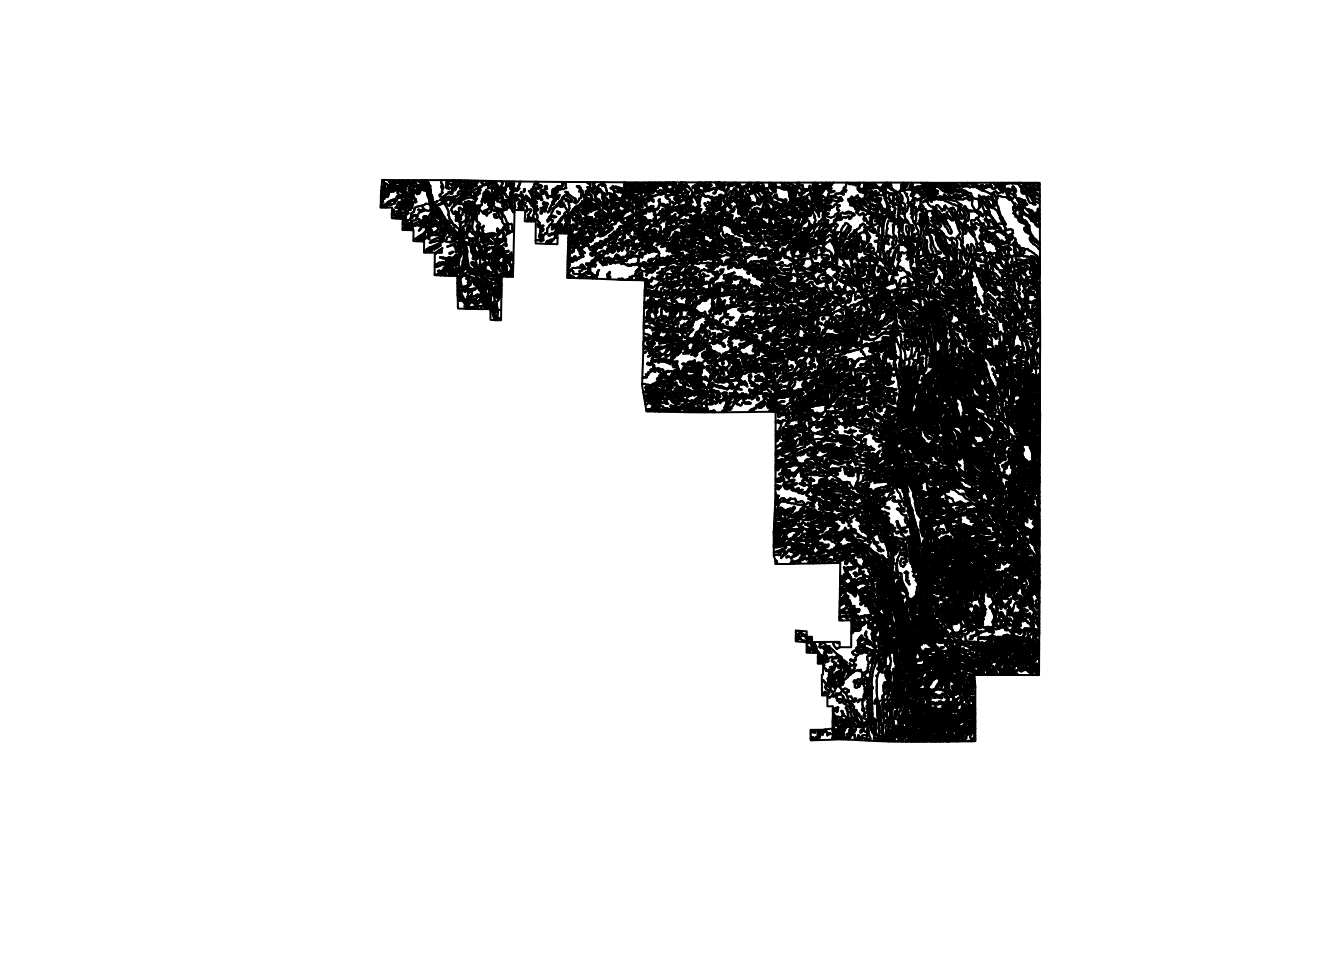
\includegraphics{SoilScript_files/figure-pdf/unnamed-chunk-2-1.pdf}

}

\end{figure}

\begin{Shaded}
\begin{Highlighting}[]
\FunctionTok{names}\NormalTok{(soils) }\CommentTok{\#get attribute data}
\end{Highlighting}
\end{Shaded}

\begin{verbatim}
 [1] "Join_Count" "TARGET_FID" "Join_Cou_1" "TARGET_F_1" "AREASYMBOL"
 [6] "SPATIALVER" "MUSYM"      "MUKEY"      "SdvOutpu_1" "SdvOutpu_2"
[11] "SdvOutpu_3" "geometry"  
\end{verbatim}

\begin{Shaded}
\begin{Highlighting}[]
\CommentTok{\#Rename original category headings to something more familiar}
\NormalTok{soils}\SpecialCharTok{$}\NormalTok{Clay }\OtherTok{\textless{}{-}}\NormalTok{ soils}\SpecialCharTok{$}\NormalTok{SdvOutpu\_1}
\NormalTok{soils}\SpecialCharTok{$}\NormalTok{pH }\OtherTok{\textless{}{-}}\NormalTok{ soils}\SpecialCharTok{$}\NormalTok{SdvOutpu\_2}
\NormalTok{soils}\SpecialCharTok{$}\NormalTok{CEC }\OtherTok{\textless{}{-}}\NormalTok{ soils}\SpecialCharTok{$}\NormalTok{SdvOutpu\_3}
\end{Highlighting}
\end{Shaded}

4.Shapefiles contain several features associated with each polygons that
collectively make up the entire layer so let's explore

\begin{Shaded}
\begin{Highlighting}[]
\NormalTok{soils }\CommentTok{\#a data frame with geometry type "polygon" associated with 10 features}
\FunctionTok{st\_bbox}\NormalTok{(soils) }\CommentTok{\#boundary box}
\FunctionTok{st\_crs}\NormalTok{(soils) }\CommentTok{\#projection information}
\NormalTok{soils[}\DecValTok{1}\NormalTok{, ] }\CommentTok{\#will bring up data associated with the first polygon}
\end{Highlighting}
\end{Shaded}

5. Select portions of the data that fit some set criteria

\begin{Shaded}
\begin{Highlighting}[]
\CommentTok{\#Highlights the areas that Percent Clay polygons are over 30\%}
\FunctionTok{plot}\NormalTok{(}\FunctionTok{st\_geometry}\NormalTok{(soils))}
\NormalTok{high.clay }\OtherTok{\textless{}{-}}\NormalTok{ soils[soils}\SpecialCharTok{$}\NormalTok{Clay}\SpecialCharTok{\textgreater{}}\DecValTok{30}\NormalTok{,]}
\FunctionTok{plot}\NormalTok{(}\FunctionTok{st\_geometry}\NormalTok{(high.clay), }\AttributeTok{border=}\StringTok{"red"}\NormalTok{, }\AttributeTok{add=}\ConstantTok{TRUE}\NormalTok{)}

\DocumentationTok{\#\#Highlights the areas that Cation Exchange Capacity is greater than 14}
\NormalTok{high.CEC}\OtherTok{\textless{}{-}}\NormalTok{ soils[soils}\SpecialCharTok{$}\NormalTok{CEC}\SpecialCharTok{\textgreater{}}\DecValTok{14}\NormalTok{,]}
\FunctionTok{plot}\NormalTok{(}\FunctionTok{st\_geometry}\NormalTok{(high.CEC), }\AttributeTok{border=}\StringTok{"green"}\NormalTok{, }\AttributeTok{add=}\ConstantTok{TRUE}\NormalTok{)}

\DocumentationTok{\#\#Highlights the areas that soil pH is greater than 8}
\NormalTok{high.pH }\OtherTok{\textless{}{-}}\NormalTok{ soils[soils}\SpecialCharTok{$}\NormalTok{pH}\SpecialCharTok{\textgreater{}}\DecValTok{8}\NormalTok{,]}
\FunctionTok{plot}\NormalTok{(}\FunctionTok{st\_geometry}\NormalTok{(high.pH), }\AttributeTok{border=}\StringTok{"yellow"}\NormalTok{, }\AttributeTok{add=}\ConstantTok{TRUE}\NormalTok{)}
\end{Highlighting}
\end{Shaded}

\begin{figure}[H]

{\centering \includegraphics{SoilScript_files/figure-pdf/unnamed-chunk-4-1.pdf}

}

\end{figure}

6. Bring in locations of harvested mule deer

\begin{Shaded}
\begin{Highlighting}[]
\CommentTok{\#Import mule deer locations from harvested animals tested for CWD}
\CommentTok{\#Note: Locations have been offset or altered so do not reflect actual locations of samples}
\NormalTok{mule }\OtherTok{\textless{}{-}} \FunctionTok{read.csv}\NormalTok{(}\StringTok{"data/MDjitterclip.csv"}\NormalTok{, }\AttributeTok{header=}\NormalTok{T)}
\NormalTok{crs}\OtherTok{\textless{}{-}}\StringTok{"+proj=utm +zone=13 +datum=WGS84 +no\_defs +towgs84=0,0,0"}
\NormalTok{coords }\OtherTok{\textless{}{-}} \FunctionTok{st\_as\_sf}\NormalTok{(mule, }\AttributeTok{coords =} \FunctionTok{c}\NormalTok{(}\StringTok{"x"}\NormalTok{, }\StringTok{"y"}\NormalTok{), }\AttributeTok{crs =} \FunctionTok{st\_crs}\NormalTok{(soils))}

\FunctionTok{plot}\NormalTok{(}\FunctionTok{st\_geometry}\NormalTok{(soils))}
\FunctionTok{plot}\NormalTok{(}\FunctionTok{st\_geometry}\NormalTok{(coords), }\AttributeTok{col=}\StringTok{"blue"}\NormalTok{,}\AttributeTok{add=}\NormalTok{T)}
\end{Highlighting}
\end{Shaded}

\begin{figure}[H]

{\centering \includegraphics{SoilScript_files/figure-pdf/unnamed-chunk-5-1.pdf}

}

\end{figure}

7. Let's generate random points with the extent of the soil layer

\begin{Shaded}
\begin{Highlighting}[]
\CommentTok{\#Sampling points in a Spatial Object "type=regular" will give a regular grid}
\NormalTok{samples}\OtherTok{\textless{}{-}}\FunctionTok{st\_sample}\NormalTok{(soils, }\DecValTok{1000}\NormalTok{, }\AttributeTok{type=}\StringTok{"random"}\NormalTok{)}

\FunctionTok{plot}\NormalTok{(}\FunctionTok{st\_geometry}\NormalTok{(soils), }\AttributeTok{col=}\StringTok{"wheat"}\NormalTok{)}
\FunctionTok{plot}\NormalTok{(}\FunctionTok{st\_geometry}\NormalTok{(coords), }\AttributeTok{col=}\StringTok{"blue"}\NormalTok{, }\AttributeTok{add=}\NormalTok{T)}
\FunctionTok{plot}\NormalTok{(}\FunctionTok{st\_geometry}\NormalTok{(samples), }\AttributeTok{col=}\StringTok{"red"}\NormalTok{, }\AttributeTok{add=}\NormalTok{T)}
\end{Highlighting}
\end{Shaded}

\begin{figure}[H]

{\centering \includegraphics{SoilScript_files/figure-pdf/unnamed-chunk-6-1.pdf}

}

\end{figure}

8. Extract and tally Clay soil types for random samples and mule deer
locations

\begin{Shaded}
\begin{Highlighting}[]
\CommentTok{\#Matches points with polygons:}
\NormalTok{soils.idx}\OtherTok{\textless{}{-}} \FunctionTok{st\_intersects}\NormalTok{(samples,soils)}
\NormalTok{soil.samples }\OtherTok{\textless{}{-}}\NormalTok{ soils[}\FunctionTok{unlist}\NormalTok{(soils.idx), }\StringTok{"Clay"}\NormalTok{, drop }\OtherTok{=} \ConstantTok{TRUE}\NormalTok{] }\CommentTok{\# drop geometry}
\CommentTok{\# locs \textless{}{-} SpatialPoints(coords)}
\CommentTok{\# locs@proj4string \textless{}{-} soils@proj4string}
\NormalTok{soils.locations}\OtherTok{\textless{}{-}} \FunctionTok{st\_intersects}\NormalTok{(coords, soils)}
\NormalTok{soils.locs }\OtherTok{\textless{}{-}}\NormalTok{ soils[}\FunctionTok{unlist}\NormalTok{(soils.locations), }\StringTok{"Clay"}\NormalTok{, drop }\OtherTok{=} \ConstantTok{TRUE}\NormalTok{]}
\CommentTok{\#Tally clay soil types for random samples}
\NormalTok{obs.tbl }\OtherTok{\textless{}{-}} \FunctionTok{table}\NormalTok{(soil.samples[soil.samples])}
\NormalTok{obs.tbl}
\end{Highlighting}
\end{Shaded}

\begin{verbatim}

   0 11.7 12.6 13.2 16.5 18.5 19.8 20.1 20.5   21 23.7 24.3 24.7 25.8 25.9 26.1 
  35   27  238   68   83   89  196    3   27   21   51   24    8    9    5   33 
26.7 37.1 
   3   14 
\end{verbatim}

\begin{Shaded}
\begin{Highlighting}[]
\CommentTok{\#Also tally soil types for each mule deer sampled}
\NormalTok{obs.tbl2 }\OtherTok{\textless{}{-}} \FunctionTok{table}\NormalTok{(soils.locs[soils.locs])}
\NormalTok{obs.tbl2}
\end{Highlighting}
\end{Shaded}

\begin{verbatim}

   0  8.7  9.7 11.5 11.7 12.1 12.6   13 13.1 16.5 18.5   21   40 
  71   31  670  237   96    1    8   89    2  236   12   30   31 
\end{verbatim}

10. Converts the counts to proportions

\begin{Shaded}
\begin{Highlighting}[]
\NormalTok{obs }\OtherTok{\textless{}{-}}\NormalTok{ obs.tbl}\SpecialCharTok{/}\FunctionTok{sum}\NormalTok{(obs.tbl)}
\NormalTok{obs}
\end{Highlighting}
\end{Shaded}

\begin{verbatim}

          0        11.7        12.6        13.2        16.5        18.5 
0.037473233 0.028907923 0.254817987 0.072805139 0.088865096 0.095289079 
       19.8        20.1        20.5          21        23.7        24.3 
0.209850107 0.003211991 0.028907923 0.022483940 0.054603854 0.025695931 
       24.7        25.8        25.9        26.1        26.7        37.1 
0.008565310 0.009635974 0.005353319 0.035331906 0.003211991 0.014989293 
\end{verbatim}

\begin{Shaded}
\begin{Highlighting}[]
\NormalTok{obs2 }\OtherTok{\textless{}{-}}\NormalTok{ obs.tbl2}\SpecialCharTok{/}\FunctionTok{sum}\NormalTok{(obs.tbl2)}
\NormalTok{obs2}
\end{Highlighting}
\end{Shaded}

\begin{verbatim}

          0         8.7         9.7        11.5        11.7        12.1 
0.046895641 0.020475561 0.442536328 0.156538970 0.063408190 0.000660502 
       12.6          13        13.1        16.5        18.5          21 
0.005284016 0.058784676 0.001321004 0.155878468 0.007926024 0.019815059 
         40 
0.020475561 
\end{verbatim}

\hypertarget{manipulate-raster-data-layer}{%
\chapter{Manipulate Raster Data
Layer}\label{manipulate-raster-data-layer}}

1. Open the script ``RasterScript.R''

2. First we need to load the packages needed for the exercise

\begin{Shaded}
\begin{Highlighting}[]
\CommentTok{\#install.packages(c("adehabitatHR","maptools","raster", "rgdal"))}
\FunctionTok{library}\NormalTok{(terra)}
\FunctionTok{library}\NormalTok{(sf)}
\FunctionTok{library}\NormalTok{(dplyr)}
\FunctionTok{library}\NormalTok{(tigris)}
\CommentTok{\#options(tigris\_use\_cache = TRUE)}
\CommentTok{\#tigris\_cache\_dir("/Users/davidwalter/Library/CloudStorage/OneDrive{-}ThePennsylvaniaStateUniversity/WalterRprojects/Manual{-}Applied{-}Spatial{-}Ecology/data")}
\CommentTok{\#\textquotesingle{}}
\CommentTok{\#install.packages("remotes")}
\CommentTok{\# remotes::install\_github(repo = "r{-}lib/devtools",}
\CommentTok{\#                               dependencies = TRUE,}
\CommentTok{\#                               upgrade = TRUE)}
\CommentTok{\# devtools::install\_github(repo = "r{-}lib/devtools",}
\CommentTok{\#                            dependencies = TRUE,}
\CommentTok{\#                            upgrade = TRUE)}
\CommentTok{\#devtools::install\_github("ropensci/FedData")}
\CommentTok{\#remotes::install\_github("ropensci/FedData")}
\FunctionTok{library}\NormalTok{(FedData)}
\FunctionTok{sessionInfo}\NormalTok{() }\CommentTok{\#Search for and confirm FedData\_4.0.0 or newer was loaded}
\end{Highlighting}
\end{Shaded}

\begin{verbatim}
R version 4.3.2 (2023-10-31)
Platform: x86_64-apple-darwin20 (64-bit)
Running under: macOS Sonoma 14.3.1

Matrix products: default
BLAS:   /Library/Frameworks/R.framework/Versions/4.3-x86_64/Resources/lib/libRblas.0.dylib 
LAPACK: /Library/Frameworks/R.framework/Versions/4.3-x86_64/Resources/lib/libRlapack.dylib;  LAPACK version 3.11.0

locale:
[1] en_US.UTF-8/en_US.UTF-8/en_US.UTF-8/C/en_US.UTF-8/en_US.UTF-8

time zone: America/New_York
tzcode source: internal

attached base packages:
[1] stats     graphics  grDevices utils     datasets  methods   base     

other attached packages:
[1] FedData_4.0.1 tigris_2.0.3  dplyr_1.1.3   sf_1.0-14     terra_1.7-46 

loaded via a namespace (and not attached):
 [1] jsonlite_1.8.7     compiler_4.3.2     tidyselect_1.2.0   Rcpp_1.0.11       
 [5] stringr_1.5.0      uuid_1.1-0         yaml_2.3.7         fastmap_1.1.1     
 [9] readr_2.1.4        R6_2.5.1           generics_0.1.3     classInt_0.4-10   
[13] knitr_1.42         tibble_3.2.1       units_0.8-4        DBI_1.1.3         
[17] tzdb_0.4.0         pillar_1.9.0       rlang_1.1.1        utf8_1.2.3        
[21] stringi_1.7.12     xfun_0.39          cli_3.6.1          magrittr_2.0.3    
[25] class_7.3-22       digest_0.6.31      grid_4.3.2         rstudioapi_0.14   
[29] hms_1.1.3          rappdirs_0.3.3     lifecycle_1.0.3    vctrs_0.6.3       
[33] KernSmooth_2.23-22 proxy_0.4-27       evaluate_0.21      glue_1.6.2        
[37] codetools_0.2-19   fansi_1.0.4        e1071_1.7-13       rmarkdown_2.21    
[41] httr_1.4.7         tools_4.3.2        pkgconfig_2.0.3    htmltools_0.5.5   
\end{verbatim}

\begin{Shaded}
\begin{Highlighting}[]
\CommentTok{\#library(adehabitatHR)}
\CommentTok{\#library(maptools)}
\end{Highlighting}
\end{Shaded}

3. Now let's have a separate section of code to include projection
information we will use throughout the exercise

\begin{Shaded}
\begin{Highlighting}[]
\NormalTok{ll.crs}\OtherTok{=}\FunctionTok{st\_crs}\NormalTok{(}\DecValTok{4269}\NormalTok{)}
\NormalTok{utm.crs }\OtherTok{\textless{}{-}} \FunctionTok{st\_crs}\NormalTok{(}\DecValTok{9001}\NormalTok{)}
\NormalTok{albers.crs }\OtherTok{\textless{}{-}} \FunctionTok{st\_crs}\NormalTok{(}\DecValTok{5070}\NormalTok{)}
\CommentTok{\#CRS of shapefile layers}
\CommentTok{\#crs \textless{}{-} CRS("+proj=aea +lat\_1=29.5 +lat\_2=45.5 +lat\_0=23 +lon\_0={-}96 +x\_0=0 }
\CommentTok{\#  +y\_0=0 +datum=NAD83 +units=m +no\_defs +ellps=GRS80 +towgs84=0,0,0")}
\CommentTok{\#CRS of raster layers}
\CommentTok{\#crs2 \textless{}{-} CRS("+proj=aea +lat\_1=29.5 +lat\_2=45.5 +lat\_0=23 +lon\_0={-}96 +x\_0=0 +y\_0=0 }
\CommentTok{\#  +ellps=GRS80 +towgs84=0,0,0,0,0,0,0 +units=m +no\_defs")}
\end{Highlighting}
\end{Shaded}

4. We will use the tigris package to downloaded statewide layers for
state and county outlines

\begin{Shaded}
\begin{Highlighting}[]
\NormalTok{st }\OtherTok{\textless{}{-}}\NormalTok{ tigris}\SpecialCharTok{::}\FunctionTok{states}\NormalTok{() }\SpecialCharTok{\%\textgreater{}\%}
\NormalTok{  dplyr}\SpecialCharTok{::}\FunctionTok{filter}\NormalTok{(GEOID }\SpecialCharTok{\textless{}} \StringTok{"60"}\NormalTok{) }\SpecialCharTok{\%\textgreater{}\%} 
\NormalTok{  tigris}\SpecialCharTok{::}\FunctionTok{shift\_geometry}\NormalTok{()}
\CommentTok{\#GEOID\textquotesingle{}s above 60 are territories and islands, etc. So I\textquotesingle{}m removing them for scaling.}
\FunctionTok{plot}\NormalTok{(}\FunctionTok{st\_geometry}\NormalTok{(st))}

\NormalTok{st }\OtherTok{\textless{}{-}} \FunctionTok{st\_transform}\NormalTok{(st, albers.crs)}
\NormalTok{SC.outline }\OtherTok{\textless{}{-}} \FunctionTok{subset}\NormalTok{(st, st}\SpecialCharTok{$}\NormalTok{NAME }\SpecialCharTok{==} \StringTok{"South Carolina"}\NormalTok{)}

\NormalTok{SCcounties }\OtherTok{\textless{}{-}} \FunctionTok{counties}\NormalTok{(}\StringTok{"South Carolina"}\NormalTok{, }\AttributeTok{cb =} \ConstantTok{TRUE}\NormalTok{)}
\NormalTok{SCcounties }\OtherTok{\textless{}{-}} \FunctionTok{st\_transform}\NormalTok{(SCcounties, albers.crs)}
\end{Highlighting}
\end{Shaded}

5. Now let's add some shapefiles to our raster specific to the military
base of interest

\begin{Shaded}
\begin{Highlighting}[]
\CommentTok{\#Load county shapefile}
\NormalTok{county}\OtherTok{\textless{}{-}} \FunctionTok{subset}\NormalTok{(SCcounties, SCcounties}\SpecialCharTok{$}\NormalTok{NAME }\SpecialCharTok{==} \StringTok{"Beaufort"}\NormalTok{)}

\CommentTok{\#Load airport runway shapefile}
\NormalTok{run}\OtherTok{\textless{}{-}}\FunctionTok{st\_read}\NormalTok{(}\StringTok{"data/RunwayAlbers.shp"}\NormalTok{)}

\CommentTok{\#Load aircraft flight pattern shapefile}
\NormalTok{path}\OtherTok{\textless{}{-}}\FunctionTok{st\_read}\NormalTok{(}\StringTok{"data/FlightImage.shp"}\NormalTok{)}

\CommentTok{\#Load aircraft flight pattern shapefile}
\NormalTok{road }\OtherTok{\textless{}{-}} \FunctionTok{st\_read}\NormalTok{(}\StringTok{"data/CountyRoadAlbers.shp"}\NormalTok{)}
\end{Highlighting}
\end{Shaded}

\begin{enumerate}
\def\labelenumi{\arabic{enumi}.}
\setcounter{enumi}{5}
\tightlist
\item
  Using county outline, we can then download National Land Cover data
  for any year of interest using the FedData package
\end{enumerate}

\begin{Shaded}
\begin{Highlighting}[]
\CommentTok{\#new.outline \textless{}{-} sf::as\_Spatial(county)\#need to do this line due to error with dplyr package}
\NormalTok{SCnlcd }\OtherTok{\textless{}{-}} \FunctionTok{get\_nlcd}\NormalTok{(}\AttributeTok{template=}\NormalTok{SC.outline, }\AttributeTok{year =} \DecValTok{2019}\NormalTok{, }\AttributeTok{label =} \StringTok{\textquotesingle{}SC\textquotesingle{}}\NormalTok{,}\AttributeTok{force.redo =}\NormalTok{ T)}
\CommentTok{\#Write raster if needed}
\CommentTok{\#writeRaster(SCnlcd, filename = "SCnlcd2019.tif", filetype = "GTiff", datatype = \textquotesingle{}INT4U\textquotesingle{},overwrite=TRUE)}
  
\FunctionTok{plot}\NormalTok{(SCnlcd)}
\FunctionTok{plot}\NormalTok{(}\FunctionTok{st\_geometry}\NormalTok{(SCcounties), }\AttributeTok{add=}\NormalTok{T, }\AttributeTok{lwd=}\DecValTok{3}\NormalTok{)}

\CommentTok{\#Import raster saved above just for demonstration}
\CommentTok{\#SCnlcd \textless{}{-}rast("SCnlcd2019.tif")}
\FunctionTok{plot}\NormalTok{(SCnlcd)}
\FunctionTok{plot}\NormalTok{(}\FunctionTok{st\_geometry}\NormalTok{(SCcounties), }\AttributeTok{add=}\NormalTok{T, }\AttributeTok{lwd=}\DecValTok{3}\NormalTok{)}
\end{Highlighting}
\end{Shaded}

7. Plot out all the shapefiles overlayed on each other with and without
the raster.

\begin{Shaded}
\begin{Highlighting}[]
\FunctionTok{plot}\NormalTok{(}\FunctionTok{st\_geometry}\NormalTok{(county))}
\FunctionTok{plot}\NormalTok{(}\FunctionTok{st\_geometry}\NormalTok{(road), }\AttributeTok{add=}\NormalTok{T)}
\FunctionTok{plot}\NormalTok{(}\FunctionTok{st\_geometry}\NormalTok{(run), }\AttributeTok{col=}\StringTok{"red"}\NormalTok{,}\AttributeTok{add=}\NormalTok{T)}
\FunctionTok{plot}\NormalTok{(}\FunctionTok{st\_geometry}\NormalTok{(path), }\AttributeTok{col=}\StringTok{"blue"}\NormalTok{,}\AttributeTok{add=}\NormalTok{T)}
\end{Highlighting}
\end{Shaded}

8. Let's reclassify NLCD layer to get fewer land cover categories to
make it easier to work with the raster.

\begin{Shaded}
\begin{Highlighting}[]
\CommentTok{\# reclassify the values into 7 groups all values between 0 and 20 equal 1, etc. while removing water (11)}
\NormalTok{m }\OtherTok{\textless{}{-}} \FunctionTok{c}\NormalTok{(}\DecValTok{0}\NormalTok{, }\DecValTok{19}\NormalTok{, }\ConstantTok{NA}\NormalTok{, }\DecValTok{20}\NormalTok{, }\DecValTok{39}\NormalTok{, }\DecValTok{1}\NormalTok{, }\DecValTok{40}\NormalTok{, }\DecValTok{50}\NormalTok{, }\DecValTok{2}\NormalTok{, }\DecValTok{51}\NormalTok{, }\DecValTok{68}\NormalTok{, }\DecValTok{3}\NormalTok{, }\DecValTok{69}\NormalTok{,}\DecValTok{79}\NormalTok{, }\DecValTok{4}\NormalTok{, }\DecValTok{80}\NormalTok{, }\DecValTok{88}\NormalTok{, }\DecValTok{5}\NormalTok{, }\DecValTok{89}\NormalTok{, }\DecValTok{99}\NormalTok{, }\DecValTok{6}\NormalTok{)}
\NormalTok{rclmat }\OtherTok{\textless{}{-}} \FunctionTok{matrix}\NormalTok{(m, }\AttributeTok{ncol=}\DecValTok{3}\NormalTok{, }\AttributeTok{byrow=}\ConstantTok{TRUE}\NormalTok{)}
\NormalTok{rc }\OtherTok{\textless{}{-}} \FunctionTok{classify}\NormalTok{(SCnlcd, rclmat)}
\FunctionTok{plot}\NormalTok{(rc)}

\CommentTok{\#Clip the raster within the county polygon for a zoomed in view then plot}
\NormalTok{clip }\OtherTok{\textless{}{-}} \FunctionTok{crop}\NormalTok{(rc, county)}
\FunctionTok{plot}\NormalTok{(clip)}
\FunctionTok{plot}\NormalTok{(}\FunctionTok{st\_geometry}\NormalTok{(county),}\AttributeTok{add=}\NormalTok{T,}\AttributeTok{lwd=}\DecValTok{2}\NormalTok{)}
\FunctionTok{plot}\NormalTok{(}\FunctionTok{st\_geometry}\NormalTok{(run),}\AttributeTok{add=}\NormalTok{T,}\AttributeTok{lwd=}\DecValTok{2}\NormalTok{, }\AttributeTok{col=}\StringTok{"red"}\NormalTok{)}
\FunctionTok{plot}\NormalTok{(}\FunctionTok{st\_geometry}\NormalTok{(path),}\AttributeTok{add=}\NormalTok{T,}\AttributeTok{lty=}\StringTok{"62"}\NormalTok{, }\AttributeTok{col=}\StringTok{"blue"}\NormalTok{)}
\FunctionTok{plot}\NormalTok{(}\FunctionTok{st\_geometry}\NormalTok{(road),}\AttributeTok{add=}\NormalTok{T,}\AttributeTok{lty=}\StringTok{"22"}\NormalTok{, }\AttributeTok{col=}\StringTok{"yellow"}\NormalTok{)}
\end{Highlighting}
\end{Shaded}

9. We can load some vulture locations to extract landcover that each
location occurs in that will be considered ``used'' habitat in resource
selection analysis.

\begin{Shaded}
\begin{Highlighting}[]
\CommentTok{\#Import bird 49 locations to R}
\NormalTok{bv49 }\OtherTok{\textless{}{-}}\FunctionTok{read.csv}\NormalTok{(}\StringTok{"data/Bird49.csv"}\NormalTok{, }\AttributeTok{header=}\NormalTok{T)}\CommentTok{\#How many bird locations?}

\NormalTok{utm.crs}\OtherTok{\textless{}{-}}\StringTok{"+proj=utm +zone=17 +ellps=WGS84"} \CommentTok{\#NOTE: If using a mac, we need to remove the N in zone 17 prior to running line below}
\CommentTok{\#Include geometry}
\NormalTok{bvspdf }\OtherTok{\textless{}{-}} \FunctionTok{st\_as\_sf}\NormalTok{(bv49, }\AttributeTok{coords =} \FunctionTok{c}\NormalTok{(}\StringTok{"x"}\NormalTok{, }\StringTok{"y"}\NormalTok{), }\AttributeTok{crs =}\NormalTok{ utm.crs)}

\FunctionTok{plot}\NormalTok{(}\FunctionTok{st\_geometry}\NormalTok{(bvspdf), }\AttributeTok{col=}\StringTok{"red"}\NormalTok{)}
\CommentTok{\#NOTE: Locations must be assigned to the UTM coordinate system prior to projection to Albers }
\CommentTok{\#so won\textquotesingle{}t overlay on veg layer at this point because veg is in Albers}
\NormalTok{bv49Albers }\OtherTok{\textless{}{-}} \FunctionTok{st\_transform}\NormalTok{(bvspdf, }\AttributeTok{crs =}\NormalTok{ albers.crs)}
\FunctionTok{plot}\NormalTok{(clip)}
\FunctionTok{plot}\NormalTok{(}\FunctionTok{st\_geometry}\NormalTok{(bv49Albers), }\AttributeTok{col=}\StringTok{"blue"}\NormalTok{,}\AttributeTok{add=}\NormalTok{T)}
\end{Highlighting}
\end{Shaded}

10. Determine which of those points lie within a cell that contains data
by using the extract function. The extract function will extract
covariate information from the raster for xy coordinates at for each
location.

\begin{Shaded}
\begin{Highlighting}[]
\NormalTok{bvspdf.df }\OtherTok{\textless{}{-}} \FunctionTok{data.frame}\NormalTok{(}\FunctionTok{st\_coordinates}\NormalTok{(bv49Albers))}
\NormalTok{bvspdf2 }\OtherTok{\textless{}{-}} \FunctionTok{st\_as\_sf}\NormalTok{(bvspdf.df, }\AttributeTok{coords=} \FunctionTok{c}\NormalTok{(}\StringTok{"X"}\NormalTok{, }\StringTok{"Y"}\NormalTok{), }\AttributeTok{crs =}\NormalTok{ albers.crs)}
\NormalTok{bvspdf.sv }\OtherTok{\textless{}{-}} \FunctionTok{vect}\NormalTok{(bvspdf2)}\CommentTok{\#Need SpatVector for extract function in terra}
\NormalTok{veg.survey}\OtherTok{\textless{}{-}}\NormalTok{terra}\SpecialCharTok{::}\FunctionTok{extract}\NormalTok{(clip, bvspdf.sv)}
\NormalTok{veg.survey}\OtherTok{\textless{}{-}}\FunctionTok{subset}\NormalTok{(veg.survey,}\SpecialCharTok{!}\FunctionTok{is.na}\NormalTok{(veg.survey}\SpecialCharTok{$}\NormalTok{Class))}
\end{Highlighting}
\end{Shaded}

11. We can also create some random points within the extent of the area
to be considered as ``available'' habitat.

\begin{Shaded}
\begin{Highlighting}[]
\DocumentationTok{\#\#First we need to create a box across the study site to generate a random sample of locations}
\NormalTok{e.box }\OtherTok{\textless{}{-}} \FunctionTok{as.polygons}\NormalTok{(clip,}\AttributeTok{extent=}\ConstantTok{TRUE}\NormalTok{)}
\NormalTok{e.box }\OtherTok{\textless{}{-}} \FunctionTok{st\_as\_sf}\NormalTok{(e.box)}
\NormalTok{Sample.points }\OtherTok{\textless{}{-}} \FunctionTok{st\_sample}\NormalTok{(e.box, }\DecValTok{1000}\NormalTok{, }\AttributeTok{type=}\StringTok{"random"}\NormalTok{)}

\FunctionTok{plot}\NormalTok{(clip)}
\FunctionTok{plot}\NormalTok{(}\FunctionTok{st\_geometry}\NormalTok{(Sample.points),}\AttributeTok{add=}\NormalTok{T)}

\CommentTok{\#Determine which of those points lie within a cell that contains data by using the extract function again.}
\NormalTok{Sample.points.sv }\OtherTok{\textless{}{-}} \FunctionTok{vect}\NormalTok{(Sample.points)}\CommentTok{\#Need SpatVector class for extract function in terra}
\NormalTok{samp.survey}\OtherTok{\textless{}{-}}\NormalTok{terra}\SpecialCharTok{::}\FunctionTok{extract}\NormalTok{(clip, Sample.points.sv)}
\NormalTok{samp.survey}\OtherTok{\textless{}{-}}\FunctionTok{subset}\NormalTok{(samp.survey,}\SpecialCharTok{!}\FunctionTok{is.na}\NormalTok{(samp.survey}\SpecialCharTok{$}\NormalTok{Class))}
\end{Highlighting}
\end{Shaded}

12. New code addition below (Update 1/7/2021) to use mapview package to
treat plotting data layers as done with GIS software. This package
enables user to zoom in and out and scroll around layer after calling a
plot function \newpage

\begin{Shaded}
\begin{Highlighting}[]
\FunctionTok{library}\NormalTok{(mapview)}
\FunctionTok{library}\NormalTok{(stars)}
\FunctionTok{mapview}\NormalTok{(}\FunctionTok{st\_as\_stars}\NormalTok{(clip)) }\SpecialCharTok{+} \FunctionTok{mapview}\NormalTok{(run) }\SpecialCharTok{+} \FunctionTok{mapview}\NormalTok{(path)}
\FunctionTok{mapview}\NormalTok{(county) }\SpecialCharTok{+} \FunctionTok{mapview}\NormalTok{(bv49Albers, }\AttributeTok{color=}\StringTok{"yellow"}\NormalTok{)}
\FunctionTok{mapview}\NormalTok{(run) }\SpecialCharTok{+}\NormalTok{ bv49Albers }\SpecialCharTok{+}\NormalTok{ road}
\end{Highlighting}
\end{Shaded}

\hypertarget{creating-a-hexagonal-polygon-grid-over-a-study-area}{%
\chapter{Creating a Hexagonal Polygon Grid Over a Study
Area}\label{creating-a-hexagonal-polygon-grid-over-a-study-area}}

1. Open the script ``GridScripts.Rmd'' and run code directly from the
script

2. First we need to load the packages needed for the exercise

\begin{Shaded}
\begin{Highlighting}[]
\FunctionTok{library}\NormalTok{(terra)}
\FunctionTok{library}\NormalTok{(sf)}
\FunctionTok{library}\NormalTok{(tigris)}
\FunctionTok{library}\NormalTok{(FedData)}
\FunctionTok{library}\NormalTok{(ggplot2)}
\end{Highlighting}
\end{Shaded}

3. Now let's have a separate section of code to include projection
information we will use throughout the exercise. In previous versions,
these lines of code were within each block of code

\begin{Shaded}
\begin{Highlighting}[]
\NormalTok{ll.crs}\OtherTok{=}\FunctionTok{st\_crs}\NormalTok{(}\DecValTok{4269}\NormalTok{)}
\NormalTok{utm.crs }\OtherTok{\textless{}{-}} \FunctionTok{st\_crs}\NormalTok{(}\DecValTok{9001}\NormalTok{)}
\NormalTok{albers.crs }\OtherTok{\textless{}{-}} \FunctionTok{st\_crs}\NormalTok{(}\DecValTok{5070}\NormalTok{)}
\end{Highlighting}
\end{Shaded}

4. We will use the tigris package to downloaded statewide layers for
state and county outlines

\begin{Shaded}
\begin{Highlighting}[]
\NormalTok{st }\OtherTok{\textless{}{-}}\NormalTok{ tigris}\SpecialCharTok{::}\FunctionTok{states}\NormalTok{() }\SpecialCharTok{\%\textgreater{}\%}
\NormalTok{  dplyr}\SpecialCharTok{::}\FunctionTok{filter}\NormalTok{(GEOID }\SpecialCharTok{\textless{}} \StringTok{"60"}\NormalTok{) }\SpecialCharTok{\%\textgreater{}\%} \CommentTok{\#GEOID\textquotesingle{}s above 60 are territories and islands, etc. So I\textquotesingle{}m removing them for scaling.}
\NormalTok{  tigris}\SpecialCharTok{::}\FunctionTok{shift\_geometry}\NormalTok{()}
\end{Highlighting}
\end{Shaded}

\begin{verbatim}

  |                                                                            
  |                                                                      |   0%
  |                                                                            
  |                                                                      |   1%
  |                                                                            
  |=                                                                     |   1%
  |                                                                            
  |=                                                                     |   2%
  |                                                                            
  |==                                                                    |   2%
  |                                                                            
  |==                                                                    |   3%
  |                                                                            
  |===                                                                   |   4%
  |                                                                            
  |===                                                                   |   5%
  |                                                                            
  |====                                                                  |   5%
  |                                                                            
  |====                                                                  |   6%
  |                                                                            
  |=====                                                                 |   7%
  |                                                                            
  |======                                                                |   8%
  |                                                                            
  |======                                                                |   9%
  |                                                                            
  |==========                                                            |  15%
  |                                                                            
  |===========                                                           |  15%
  |                                                                            
  |===========                                                           |  16%
  |                                                                            
  |============                                                          |  17%
  |                                                                            
  |============                                                          |  18%
  |                                                                            
  |=============                                                         |  18%
  |                                                                            
  |=============                                                         |  19%
  |                                                                            
  |==============                                                        |  20%
  |                                                                            
  |===============                                                       |  21%
  |                                                                            
  |================                                                      |  23%
  |                                                                            
  |============================                                          |  39%
  |                                                                            
  |=======================================                               |  56%
  |                                                                            
  |===================================================                   |  73%
  |                                                                            
  |==============================================================        |  89%
  |                                                                            
  |======================================================================| 100%
\end{verbatim}

\begin{Shaded}
\begin{Highlighting}[]
\FunctionTok{plot}\NormalTok{(}\FunctionTok{st\_geometry}\NormalTok{(st))}
\end{Highlighting}
\end{Shaded}

\begin{figure}[H]

{\centering \includegraphics{GridScripts_files/figure-pdf/unnamed-chunk-3-1.pdf}

}

\end{figure}

\begin{Shaded}
\begin{Highlighting}[]
\NormalTok{st }\OtherTok{\textless{}{-}} \FunctionTok{st\_transform}\NormalTok{(st, utm.crs)}
\NormalTok{CO.outline }\OtherTok{\textless{}{-}} \FunctionTok{subset}\NormalTok{(st, st}\SpecialCharTok{$}\NormalTok{NAME }\SpecialCharTok{==} \StringTok{"Colorado"}\NormalTok{)}

\NormalTok{COcounties }\OtherTok{\textless{}{-}} \FunctionTok{counties}\NormalTok{(}\StringTok{"Colorado"}\NormalTok{, }\AttributeTok{cb =} \ConstantTok{TRUE}\NormalTok{)}
\end{Highlighting}
\end{Shaded}

\begin{verbatim}

  |                                                                            
  |                                                                      |   0%
  |                                                                            
  |=                                                                     |   1%
  |                                                                            
  |=                                                                     |   2%
  |                                                                            
  |==                                                                    |   2%
  |                                                                            
  |==                                                                    |   3%
  |                                                                            
  |========                                                              |  11%
  |                                                                            
  |==================                                                    |  25%
  |                                                                            
  |===========================                                           |  39%
  |                                                                            
  |===================================                                   |  50%
  |                                                                            
  |====================================                                  |  51%
  |                                                                            
  |=======================================                               |  55%
  |                                                                            
  |==========================================                            |  60%
  |                                                                            
  |===============================================                       |  68%
  |                                                                            
  |=========================================================             |  82%
  |                                                                            
  |==========================================================            |  83%
  |                                                                            
  |==========================================================            |  84%
  |                                                                            
  |===========================================================           |  84%
  |                                                                            
  |============================================================          |  86%
  |                                                                            
  |=============================================================         |  87%
  |                                                                            
  |==============================================================        |  88%
  |                                                                            
  |==============================================================        |  89%
  |                                                                            
  |===============================================================       |  89%
  |                                                                            
  |===============================================================       |  90%
  |                                                                            
  |===============================================================       |  91%
  |                                                                            
  |================================================================      |  91%
  |                                                                            
  |================================================================      |  92%
  |                                                                            
  |=================================================================     |  92%
  |                                                                            
  |=================================================================     |  93%
  |                                                                            
  |====================================================================  |  97%
  |                                                                            
  |====================================================================  |  98%
  |                                                                            
  |===================================================================== |  98%
  |                                                                            
  |======================================================================| 100%
\end{verbatim}

\begin{Shaded}
\begin{Highlighting}[]
\NormalTok{COcounties }\OtherTok{\textless{}{-}} \FunctionTok{st\_transform}\NormalTok{(COcounties, utm.crs)}
\FunctionTok{plot}\NormalTok{(}\FunctionTok{st\_geometry}\NormalTok{(COcounties))}
\end{Highlighting}
\end{Shaded}

\begin{figure}[H]

{\centering \includegraphics{GridScripts_files/figure-pdf/unnamed-chunk-3-2.pdf}

}

\end{figure}

\begin{Shaded}
\begin{Highlighting}[]
\CommentTok{\#Import the location from earlier exercise}
\NormalTok{muleys }\OtherTok{\textless{}{-}}\FunctionTok{read.csv}\NormalTok{(}\StringTok{"data/muleysexample.csv"}\NormalTok{, }\AttributeTok{header=}\NormalTok{T)}

\CommentTok{\#Remove outlier locations}
\NormalTok{coords }\OtherTok{\textless{}{-}} \FunctionTok{st\_as\_sf}\NormalTok{(muleys, }\AttributeTok{coords =} \FunctionTok{c}\NormalTok{(}\StringTok{"Long"}\NormalTok{, }\StringTok{"Lat"}\NormalTok{), }\AttributeTok{crs =}\NormalTok{ ll.crs)}
\FunctionTok{plot}\NormalTok{(}\FunctionTok{st\_geometry}\NormalTok{(coords),}\AttributeTok{axes=}\NormalTok{T)}
\end{Highlighting}
\end{Shaded}

\begin{figure}[H]

{\centering \includegraphics{GridScripts_files/figure-pdf/unnamed-chunk-3-3.pdf}

}

\end{figure}

\begin{Shaded}
\begin{Highlighting}[]
\NormalTok{deer.spdf }\OtherTok{\textless{}{-}} \FunctionTok{st\_crop}\NormalTok{(coords, }\AttributeTok{xmin=}\SpecialCharTok{{-}}\FloatTok{107.0}\NormalTok{,}\AttributeTok{xmax=}\SpecialCharTok{{-}}\FloatTok{110.5}\NormalTok{,}\AttributeTok{ymin=}\FloatTok{37.8}\NormalTok{,}\AttributeTok{ymax=}\FloatTok{39.0}\NormalTok{)}\CommentTok{\#Visually identified based on previous plot}
\FunctionTok{plot}\NormalTok{(}\FunctionTok{st\_geometry}\NormalTok{(deer.spdf),}\AttributeTok{axes=}\NormalTok{T)}
\end{Highlighting}
\end{Shaded}

\begin{figure}[H]

{\centering 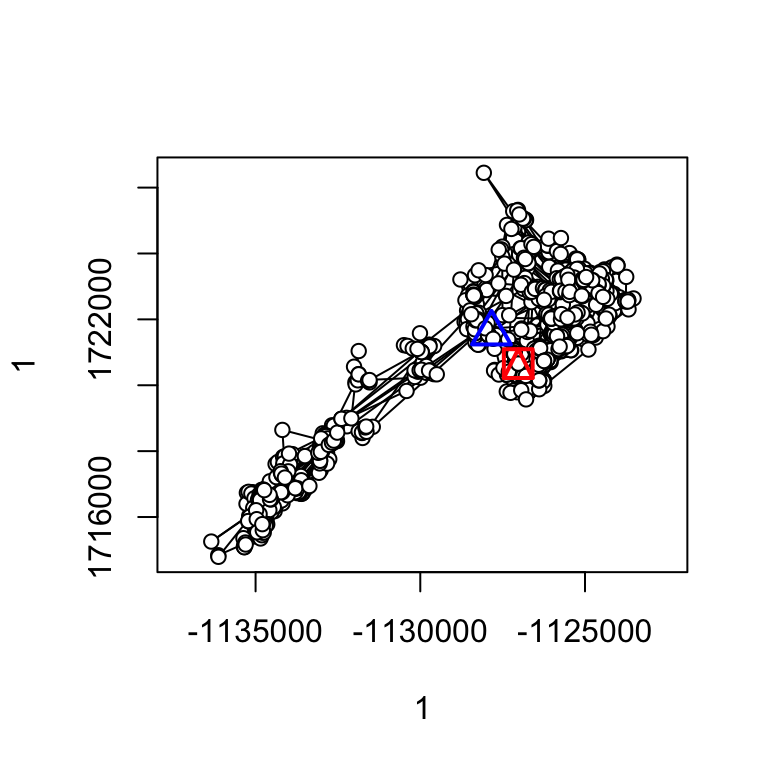
\includegraphics{GridScripts_files/figure-pdf/unnamed-chunk-3-4.pdf}

}

\end{figure}

\begin{Shaded}
\begin{Highlighting}[]
\NormalTok{deer.spdf }\OtherTok{\textless{}{-}}\FunctionTok{st\_transform}\NormalTok{(deer.spdf, }\AttributeTok{crs=}\NormalTok{utm.crs)}
\end{Highlighting}
\end{Shaded}

5. Now lets extract counties within the extent of the mule deer
locations

\begin{Shaded}
\begin{Highlighting}[]
\NormalTok{int }\OtherTok{\textless{}{-}} \FunctionTok{st\_intersection}\NormalTok{(COcounties,deer.spdf)}
\NormalTok{clipped }\OtherTok{\textless{}{-}}\NormalTok{ COcounties[int,]}
\FunctionTok{plot}\NormalTok{(}\FunctionTok{st\_geometry}\NormalTok{(clipped))}
\FunctionTok{plot}\NormalTok{(}\FunctionTok{st\_geometry}\NormalTok{(deer.spdf), }\AttributeTok{add=}\NormalTok{T)}
\end{Highlighting}
\end{Shaded}

\begin{figure}[H]

{\centering \includegraphics{GridScripts_files/figure-pdf/unnamed-chunk-4-1.pdf}

}

\end{figure}

6. We also can create a hexagonal grid across the study site

\begin{Shaded}
\begin{Highlighting}[]
\NormalTok{grid\_spacing }\OtherTok{\textless{}{-}} \DecValTok{1500}
\NormalTok{HexPols }\OtherTok{\textless{}{-}} \FunctionTok{st\_make\_grid}\NormalTok{(clipped, }\AttributeTok{square =}\NormalTok{ F, }\AttributeTok{cellsize =} \FunctionTok{c}\NormalTok{(grid\_spacing, grid\_spacing)) }\SpecialCharTok{\%\textgreater{}\%} \CommentTok{\# the grid, covering bounding box}
  \FunctionTok{st\_intersection}\NormalTok{(clipped) }
  
\FunctionTok{plot}\NormalTok{(}\FunctionTok{st\_geometry}\NormalTok{(clipped))}
\FunctionTok{plot}\NormalTok{(}\FunctionTok{st\_geometry}\NormalTok{(HexPols),}\AttributeTok{add=}\NormalTok{T)}
\end{Highlighting}
\end{Shaded}

\begin{figure}[H]

{\centering \includegraphics{GridScripts_files/figure-pdf/unnamed-chunk-5-1.pdf}

}

\end{figure}

7. Create this hexagonal grid across our study site by zooming into deer
locations

\begin{Shaded}
\begin{Highlighting}[]
\CommentTok{\#Import the study site zoomed in shapefile}
\NormalTok{study.zoom}\OtherTok{\textless{}{-}}\FunctionTok{st\_read}\NormalTok{(}\StringTok{"data/MDzoom.shp"}\NormalTok{)}
\end{Highlighting}
\end{Shaded}

\begin{verbatim}
Reading layer `MDzoom' from data source 
  `/Users/davidwalter/Library/CloudStorage/OneDrive-ThePennsylvaniaStateUniversity/WalterRprojects/Manual-of-Applied-Spatial-Ecology/data/MDzoom.shp' 
  using driver `ESRI Shapefile'
Simple feature collection with 1 feature and 1 field
Geometry type: POLYGON
Dimension:     XY
Bounding box:  xmin: -109.2433 ymin: 37.56257 xmax: -108.6488 ymax: 37.95425
Geodetic CRS:  WGS 84
\end{verbatim}

\begin{Shaded}
\begin{Highlighting}[]
\NormalTok{study.zoom }\OtherTok{\textless{}{-}} \FunctionTok{st\_transform}\NormalTok{(study.zoom, }\AttributeTok{crs=}\NormalTok{utm.crs)}

\CommentTok{\#Create new hexagonal grid}
\NormalTok{grid\_spacing }\OtherTok{\textless{}{-}} \DecValTok{1500}
\NormalTok{HexPols }\OtherTok{\textless{}{-}} \FunctionTok{st\_make\_grid}\NormalTok{(study.zoom, }\AttributeTok{square =}\NormalTok{ F, }\AttributeTok{cellsize =} \FunctionTok{c}\NormalTok{(grid\_spacing, grid\_spacing)) }\SpecialCharTok{\%\textgreater{}\%} \CommentTok{\# the grid, covering bounding box}
  \FunctionTok{st\_intersection}\NormalTok{(study.zoom) }\SpecialCharTok{\%\textgreater{}\%}
    \FunctionTok{cbind}\NormalTok{(}\FunctionTok{data.frame}\NormalTok{(}\AttributeTok{ID =} \FunctionTok{sprintf}\NormalTok{(}\FunctionTok{paste}\NormalTok{(}\StringTok{"GID\%0"}\NormalTok{,}\FunctionTok{nchar}\NormalTok{(}\FunctionTok{length}\NormalTok{(.)),}\StringTok{"d"}\NormalTok{,}\AttributeTok{sep=}\StringTok{""}\NormalTok{), }\DecValTok{1}\SpecialCharTok{:}\FunctionTok{length}\NormalTok{(.)))) }\SpecialCharTok{\%\textgreater{}\%}
    \FunctionTok{st\_sf}\NormalTok{()}
\FunctionTok{plot}\NormalTok{(}\FunctionTok{st\_geometry}\NormalTok{(study.zoom))}
\FunctionTok{plot}\NormalTok{(}\FunctionTok{st\_geometry}\NormalTok{(HexPols),}\AttributeTok{add=}\NormalTok{T)}
\end{Highlighting}
\end{Shaded}

\begin{figure}[H]

{\centering \includegraphics{GridScripts_files/figure-pdf/unnamed-chunk-6-1.pdf}

}

\end{figure}

\begin{Shaded}
\begin{Highlighting}[]
\CommentTok{\#Now add labels to each hexagon for unique ID}
\NormalTok{hex.centroids }\OtherTok{\textless{}{-}}\NormalTok{ sf}\SpecialCharTok{::}\FunctionTok{st\_point\_on\_surface}\NormalTok{(HexPols)}
\NormalTok{hex\_coords }\OtherTok{\textless{}{-}} \FunctionTok{as.data.frame}\NormalTok{(sf}\SpecialCharTok{::}\FunctionTok{st\_coordinates}\NormalTok{(hex.centroids))}
\NormalTok{hex\_coords}\SpecialCharTok{$}\NormalTok{NAME }\OtherTok{\textless{}{-}}\NormalTok{ HexPols}\SpecialCharTok{$}\NormalTok{ID}
\FunctionTok{ggplot}\NormalTok{() }\SpecialCharTok{+}
  \FunctionTok{geom\_sf}\NormalTok{(}\AttributeTok{data =}\NormalTok{ HexPols) }\SpecialCharTok{+}
  \FunctionTok{geom\_text}\NormalTok{(}\AttributeTok{data =}\NormalTok{ hex\_coords, }\FunctionTok{aes}\NormalTok{(X, Y, }\AttributeTok{label =}\NormalTok{ NAME), }\AttributeTok{colour =}\StringTok{"black"}\NormalTok{)}
\end{Highlighting}
\end{Shaded}

\begin{figure}[H]

{\centering \includegraphics{GridScripts_files/figure-pdf/unnamed-chunk-6-2.pdf}

}

\end{figure}

8. We can intersect the mule deer locations with the polygon shapefile
(i.e., county) they occurred in Hexagon ID if needed

\begin{Shaded}
\begin{Highlighting}[]
\NormalTok{o }\OtherTok{=} \FunctionTok{st\_intersection}\NormalTok{(deer.spdf,COcounties)}
\end{Highlighting}
\end{Shaded}

\begin{verbatim}
Warning: attribute variables are assumed to be spatially constant throughout
all geometries
\end{verbatim}

9. As an alternative to importing a polygon that we created in ArcMap
above, we can create a polygon in R using the coordinates of the
boundary box of the area of interest. In our case here, the bounding box
will be the mule deer locations.

\begin{Shaded}
\begin{Highlighting}[]
\NormalTok{bb }\OtherTok{\textless{}{-}} \FunctionTok{st\_bbox}\NormalTok{(deer.spdf) }\SpecialCharTok{\%\textgreater{}\%} \FunctionTok{st\_as\_sfc}\NormalTok{()}
\CommentTok{\#bb \textless{}{-} cbind(x=c({-}108.83966,{-}108.83966,{-}108.9834,{-}108.9834, {-}108.83966), }
\CommentTok{\#  y=c(37.8142, 37.86562,37.86562,37.8142,37.8142))}
\FunctionTok{plot}\NormalTok{(}\FunctionTok{st\_geometry}\NormalTok{(bb))}
\FunctionTok{plot}\NormalTok{(}\FunctionTok{st\_geometry}\NormalTok{(deer.spdf),}\AttributeTok{col=}\StringTok{"red"}\NormalTok{,}\AttributeTok{add=}\NormalTok{T)}
\end{Highlighting}
\end{Shaded}

\begin{figure}[H]

{\centering 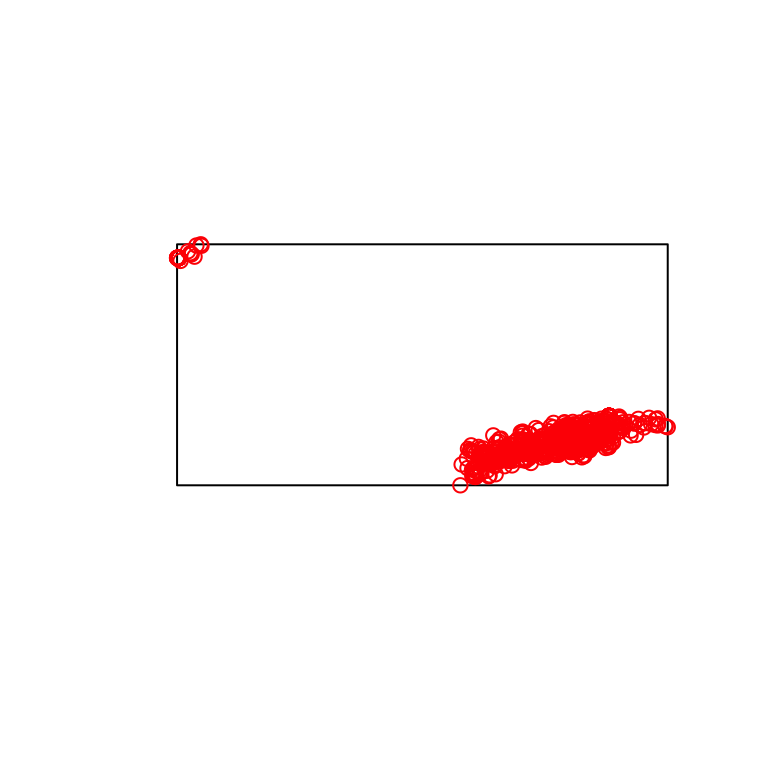
\includegraphics{GridScripts_files/figure-pdf/unnamed-chunk-8-1.pdf}

}

\end{figure}

10. Now make practical use of the new bounding box we created by
clipping a larger raster dataset. A smaller raster dataset runs analyses
faster, provides a zoomed in view of mule deer locations and vegetation,
and is just easier to work with.

\begin{Shaded}
\begin{Highlighting}[]
\CommentTok{\#Load vegetation raster layer textfile clipped in ArcMap }
\NormalTok{veg }\OtherTok{\textless{}{-}}\FunctionTok{raster}\NormalTok{(}\StringTok{"extentnlcd2.txt"}\NormalTok{)}
\FunctionTok{plot}\NormalTok{(veg)}
\FunctionTok{class}\NormalTok{(veg)}
\end{Highlighting}
\end{Shaded}

\begin{Shaded}
\begin{Highlighting}[]
\CommentTok{\#Clip using the raster imported with "raster" package}
\NormalTok{bbclip }\OtherTok{\textless{}{-}} \FunctionTok{st\_crop}\NormalTok{(veg, bb)}
\NormalTok{veg}
\end{Highlighting}
\end{Shaded}

\begin{Shaded}
\begin{Highlighting}[]
\CommentTok{\#WON\textquotesingle{}T WORK because projections are not the same, WHY?}
\CommentTok{\#Let\textquotesingle{}s check projections of layers we are working with now.}
\FunctionTok{st\_crs}\NormalTok{(MDclip)}
\FunctionTok{st\_crs}\NormalTok{(deer.spdf)}
\FunctionTok{st\_crs}\NormalTok{(SP)}
\FunctionTok{st\_crs}\NormalTok{(veg)}
\end{Highlighting}
\end{Shaded}

11. We need to have all layers in same projection so project the
deer.spdf to Albers and then clip vegetation layer with new polygon we
created in the Albers projection.

\begin{Shaded}
\begin{Highlighting}[]
\NormalTok{deer.albers }\OtherTok{\textless{}{-}}\FunctionTok{st\_transform}\NormalTok{(deer.spdf, }\AttributeTok{crs=}\NormalTok{albers.crs)}
\NormalTok{bb.albers }\OtherTok{\textless{}{-}} \FunctionTok{st\_bbox}\NormalTok{(deer.albers) }\SpecialCharTok{\%\textgreater{}\%} \FunctionTok{st\_as\_sfc}\NormalTok{()}
\CommentTok{\#Check to see all our layers are now in Albers projection}
\FunctionTok{st\_crs}\NormalTok{(veg)}
\FunctionTok{st\_crs}\NormalTok{(deer.albers)}
\FunctionTok{st\_crs}\NormalTok{(bb.albers)}

\CommentTok{\#Clip using the raster imported with "raster" package }
\NormalTok{bbclip }\OtherTok{\textless{}{-}} \FunctionTok{st\_crop}\NormalTok{(veg, AlbersSP)}
\FunctionTok{plot}\NormalTok{(bbclip)}
\FunctionTok{plot}\NormalTok{(}\FunctionTok{st\_geometry}\NormalTok{(deer.albers), }\AttributeTok{col=}\StringTok{"red"}\NormalTok{, }\AttributeTok{add=}\NormalTok{T)}
\FunctionTok{plot}\NormalTok{(}\FunctionTok{st\_geometry}\NormalTok{(bb.albers), }\AttributeTok{lwd=}\DecValTok{5}\NormalTok{, }\AttributeTok{add=}\NormalTok{T)}
\end{Highlighting}
\end{Shaded}

\hypertarget{creating-a-square-polygon-grid-over-a-study-area}{%
\chapter{Creating a Square Polygon Grid Over a Study
Area}\label{creating-a-square-polygon-grid-over-a-study-area}}

1. Open the script ``GridSystem2Script.Rmd'' and run code directly from
the script

2. First we need to load the packages needed for the exercise

\begin{Shaded}
\begin{Highlighting}[]
\FunctionTok{library}\NormalTok{(sf)}
\FunctionTok{library}\NormalTok{(terra)}
\FunctionTok{library}\NormalTok{(adehabitatMA)}
\FunctionTok{library}\NormalTok{(FedData)}
\end{Highlighting}
\end{Shaded}

3. Now let's have a separate section of code to include projection
information we will use throughout the exercise. In previous versions,
these lines of code were within each block of code

\begin{Shaded}
\begin{Highlighting}[]
\NormalTok{ll.crs }\OtherTok{\textless{}{-}} \FunctionTok{st\_crs}\NormalTok{(}\DecValTok{4269}\NormalTok{)}
\NormalTok{utm.crs }\OtherTok{\textless{}{-}} \FunctionTok{st\_crs}\NormalTok{(}\DecValTok{9001}\NormalTok{)}
\NormalTok{albers.crs }\OtherTok{\textless{}{-}} \FunctionTok{st\_crs}\NormalTok{(}\DecValTok{5070}\NormalTok{)}
\end{Highlighting}
\end{Shaded}

4. We need to have all layers in same projection so import, create, and
remove outliers for mule deer locations then project all to the Albers
projection as we did previously.

\begin{Shaded}
\begin{Highlighting}[]
\CommentTok{\#Import the location from earlier exercise}
\NormalTok{muleys }\OtherTok{\textless{}{-}}\FunctionTok{read.csv}\NormalTok{(}\StringTok{"data/muleysexample.csv"}\NormalTok{, }\AttributeTok{header=}\NormalTok{T)}

\CommentTok{\#Remove outlier locations}
\NormalTok{coords }\OtherTok{\textless{}{-}} \FunctionTok{st\_as\_sf}\NormalTok{(muleys, }\AttributeTok{coords =} \FunctionTok{c}\NormalTok{(}\StringTok{"Long"}\NormalTok{, }\StringTok{"Lat"}\NormalTok{), }\AttributeTok{crs =}\NormalTok{ ll.crs)}
\FunctionTok{plot}\NormalTok{(}\FunctionTok{st\_geometry}\NormalTok{(coords),}\AttributeTok{axes=}\NormalTok{T)}
\end{Highlighting}
\end{Shaded}

\begin{figure}[H]

{\centering \includegraphics{GridSystem2Script_files/figure-pdf/unnamed-chunk-3-1.pdf}

}

\end{figure}

\begin{Shaded}
\begin{Highlighting}[]
\NormalTok{deer.spdf }\OtherTok{\textless{}{-}} \FunctionTok{st\_crop}\NormalTok{(coords, }\AttributeTok{xmin=}\SpecialCharTok{{-}}\FloatTok{107.0}\NormalTok{,}\AttributeTok{xmax=}\SpecialCharTok{{-}}\FloatTok{110.5}\NormalTok{,}\AttributeTok{ymin=}\FloatTok{37.8}\NormalTok{,}\AttributeTok{ymax=}\FloatTok{39.0}\NormalTok{)}\CommentTok{\#Visually identified based on previous plot}
\FunctionTok{plot}\NormalTok{(}\FunctionTok{st\_geometry}\NormalTok{(deer.spdf),}\AttributeTok{axes=}\NormalTok{T)}
\end{Highlighting}
\end{Shaded}

\begin{figure}[H]

{\centering \includegraphics{GridSystem2Script_files/figure-pdf/unnamed-chunk-3-2.pdf}

}

\end{figure}

\begin{Shaded}
\begin{Highlighting}[]
\NormalTok{deer.spdf }\OtherTok{\textless{}{-}}\FunctionTok{st\_transform}\NormalTok{(deer.spdf, }\AttributeTok{crs=}\NormalTok{utm.crs)}

\CommentTok{\#Project deer.spdf to Albers as in previous exercise}
\NormalTok{deer.albers }\OtherTok{\textless{}{-}}\FunctionTok{st\_transform}\NormalTok{(deer.spdf, }\AttributeTok{crs=}\NormalTok{albers.crs)}
\FunctionTok{plot}\NormalTok{(}\FunctionTok{st\_geometry}\NormalTok{(deer.albers,}\AttributeTok{axes=}\NormalTok{T))}
\end{Highlighting}
\end{Shaded}

\begin{figure}[H]

{\centering \includegraphics{GridSystem2Script_files/figure-pdf/unnamed-chunk-3-3.pdf}

}

\end{figure}

5. Create points for x and y from the bounding box of all mule deer
locations with 1500 m spacing between each point.

\begin{Shaded}
\begin{Highlighting}[]
\NormalTok{bb }\OtherTok{\textless{}{-}} \FunctionTok{st\_bbox}\NormalTok{(deer.albers) }\SpecialCharTok{\%\textgreater{}\%} \FunctionTok{st\_as\_sfc}\NormalTok{()}
\CommentTok{\#bb \textless{}{-} cbind(x=c({-}108.83966,{-}108.83966,{-}108.9834,{-}108.9834, {-}108.83966), }
\CommentTok{\#  y=c(37.8142, 37.86562,37.86562,37.8142,37.8142))}
\FunctionTok{plot}\NormalTok{(}\FunctionTok{st\_geometry}\NormalTok{(bb))}
\FunctionTok{plot}\NormalTok{(}\FunctionTok{st\_geometry}\NormalTok{(deer.albers),}\AttributeTok{col=}\StringTok{"red"}\NormalTok{,}\AttributeTok{add=}\NormalTok{T)}
\end{Highlighting}
\end{Shaded}

\begin{figure}[H]

{\centering \includegraphics{GridSystem2Script_files/figure-pdf/unnamed-chunk-4-1.pdf}

}

\end{figure}

6. Create a grid of all pairs of coordinates (as a data.frame) using the
``expand grid'' function and then make it a gridded object.

\begin{Shaded}
\begin{Highlighting}[]
\NormalTok{grid\_spacing }\OtherTok{\textless{}{-}} \DecValTok{500}
\NormalTok{GridPols }\OtherTok{\textless{}{-}} \FunctionTok{st\_make\_grid}\NormalTok{(bb, }\AttributeTok{square =}\NormalTok{ T, }\AttributeTok{cellsize =} \FunctionTok{c}\NormalTok{(grid\_spacing, grid\_spacing)) }\SpecialCharTok{\%\textgreater{}\%} \CommentTok{\# the grid, covering bounding box}
  \FunctionTok{st\_intersection}\NormalTok{(bb) }\SpecialCharTok{\%\textgreater{}\%}
    \FunctionTok{cbind}\NormalTok{(}\FunctionTok{data.frame}\NormalTok{(}\AttributeTok{ID =} \FunctionTok{sprintf}\NormalTok{(}\FunctionTok{paste}\NormalTok{(}\StringTok{"GID\%0"}\NormalTok{,}\FunctionTok{nchar}\NormalTok{(}\FunctionTok{length}\NormalTok{(.)),}\StringTok{"d"}\NormalTok{,}\AttributeTok{sep=}\StringTok{""}\NormalTok{), }\DecValTok{1}\SpecialCharTok{:}\FunctionTok{length}\NormalTok{(.)))) }\SpecialCharTok{\%\textgreater{}\%}
    \FunctionTok{st\_sf}\NormalTok{()}
\FunctionTok{plot}\NormalTok{(}\FunctionTok{st\_geometry}\NormalTok{(bb))}
\FunctionTok{plot}\NormalTok{(}\FunctionTok{st\_geometry}\NormalTok{(GridPols),}\AttributeTok{add=}\NormalTok{T)}
\end{Highlighting}
\end{Shaded}

\begin{figure}[H]

{\centering \includegraphics{GridSystem2Script_files/figure-pdf/unnamed-chunk-5-1.pdf}

}

\end{figure}

7. Similar to the hexagonal grid, identify the cell ID that contains
each mule deer location.

\begin{Shaded}
\begin{Highlighting}[]
\NormalTok{o }\OtherTok{=} \FunctionTok{st\_intersection}\NormalTok{(deer.albers,GridPols)}
\end{Highlighting}
\end{Shaded}

\begin{verbatim}
Warning: attribute variables are assumed to be spatially constant throughout
all geometries
\end{verbatim}

\begin{Shaded}
\begin{Highlighting}[]
\FunctionTok{head}\NormalTok{(o)}
\end{Highlighting}
\end{Shaded}

\begin{verbatim}
Simple feature collection with 6 features and 21 fields
Geometry type: POINT
Dimension:     XY
Bounding box:  xmin: -1120488 ymin: 1718097 xmax: -1120110 ymax: 1718916
Projected CRS: NAD83 / Conus Albers
         DateTimeAnimalID id  Serial            Acq_Time              Acq_ST
197 D82011.10.20 12:00:00 D8 647578A 2011.10.20 12:00:40 2011.10.20 12:00:00
230 D82011.10.24 15:00:00 D8 647578A 2011.10.24 15:00:48 2011.10.24 15:00:00
231 D82011.10.24 18:00:00 D8 647578A 2011.10.24 18:01:58 2011.10.24 18:00:00
232 D82011.10.24 21:00:00 D8 647578A 2011.10.24 21:00:49 2011.10.24 21:00:00
333 D82011.11.06 18:00:00 D8 647578A 2011.11.06 18:01:04 2011.11.06 18:00:00
328 D82011.11.06 03:00:00 D8 647578A 2011.11.06 03:00:52 2011.11.06 03:00:00
             GPSFixTime      GPSFixAtt UTM_Zone       Y      X GPS_Alt
197 2011.10.20 12:00:40 Succeeded (3D)      12S 4187300 685838    2176
230 2011.10.24 15:00:48 Succeeded (3D)      12S 4187827 686114    2237
231 2011.10.24 18:01:58 Succeeded (3D)      12S 4187807 686078    2217
232 2011.10.24 21:00:49 Succeeded (3D)      12S 4187812 686107    2233
333 2011.11.06 18:01:04 Succeeded (3D)      12S 4187805 686032    2222
328 2011.11.06 03:00:52 Succeeded (3D)      12S 4188096 685684    2173
    GPS_Speed GPSHeading GPSHorizEr GPS_PD    GPS_SB GPS_SC GPS_NT Pre_Data
197      0.05        0.7      18.46    3.4   4227808      6     40       No
230      0.07        0.7      24.00    2.8 134299840      5     48       No
231      0.04        0.7     108.00    4.7      2314      4    118       No
232      0.06      348.0      24.00    3.8  16779290      5     49       No
333      0.03        0.7      45.00    3.3     66314      5     64       No
328      0.02        0.7      48.00    3.8   1318948      5     52       No
    Error     ID                 geometry
197    NA GID015 POINT (-1120464 1718097)
230    NA GID016 POINT (-1120110 1718579)
231    NA GID016 POINT (-1120149 1718566)
232    NA GID016 POINT (-1120119 1718566)
333    NA GID016 POINT (-1120193 1718571)
328    NA GID040 POINT (-1120488 1718916)
\end{verbatim}

8. If we get some NA errors because our grid does not encompass all mule
deer locations then we can expand the grid size extending beyond our
locations.

\begin{Shaded}
\begin{Highlighting}[]
\CommentTok{\# Create vectors of the x and y points using boundary box created around deer locations}
\NormalTok{bb1 }\OtherTok{\textless{}{-}} \FunctionTok{st\_bbox}\NormalTok{(GridPols)}
     
\NormalTok{increment }\OtherTok{=} \DecValTok{2000}
\NormalTok{minx}\OtherTok{=}\NormalTok{(}\FunctionTok{min}\NormalTok{(bb1}\SpecialCharTok{$}\NormalTok{xmin)}\SpecialCharTok{{-}}\NormalTok{(increment))}
\NormalTok{maxx}\OtherTok{=}\NormalTok{(}\FunctionTok{max}\NormalTok{(bb1}\SpecialCharTok{$}\NormalTok{xmax)}\SpecialCharTok{+}\NormalTok{(increment))}
\NormalTok{miny}\OtherTok{=}\NormalTok{(}\FunctionTok{min}\NormalTok{(bb1}\SpecialCharTok{$}\NormalTok{ymin)}\SpecialCharTok{{-}}\NormalTok{(increment))}
\NormalTok{maxy}\OtherTok{=}\NormalTok{(}\FunctionTok{max}\NormalTok{(bb1}\SpecialCharTok{$}\NormalTok{ymax)}\SpecialCharTok{+}\NormalTok{(increment))}
  \CommentTok{\# Create vectors of the x and y points using mean size of deer home range of X square kilometers}
\NormalTok{x}\OtherTok{=}\FunctionTok{seq}\NormalTok{(}\AttributeTok{from=}\NormalTok{minx,}\AttributeTok{to=}\NormalTok{maxx,}\AttributeTok{by=}\NormalTok{increment)}
\NormalTok{y}\OtherTok{=}\FunctionTok{seq}\NormalTok{(}\AttributeTok{from=}\NormalTok{miny,}\AttributeTok{to=}\NormalTok{maxy,}\AttributeTok{by=}\NormalTok{increment)}
\CommentTok{\# Create a grid of all pairs of coordinates (as a data.frame) }
\NormalTok{xy}\OtherTok{=}\FunctionTok{expand.grid}\NormalTok{(}\AttributeTok{x=}\NormalTok{x,}\AttributeTok{y=}\NormalTok{y)}
\NormalTok{grid.pts}\OtherTok{\textless{}{-}}\FunctionTok{st\_as\_sf}\NormalTok{(xy, }\AttributeTok{coords =} \FunctionTok{c}\NormalTok{(}\StringTok{"x"}\NormalTok{,}\StringTok{"y"}\NormalTok{),}\AttributeTok{crs =}\NormalTok{ albers.crs)}
\FunctionTok{plot}\NormalTok{(}\FunctionTok{st\_geometry}\NormalTok{(grid.pts))}
\end{Highlighting}
\end{Shaded}

\begin{figure}[H]

{\centering \includegraphics{GridSystem2Script_files/figure-pdf/unnamed-chunk-7-1.pdf}

}

\end{figure}

\begin{Shaded}
\begin{Highlighting}[]
\NormalTok{GridPols2 }\OtherTok{\textless{}{-}} \FunctionTok{st\_make\_grid}\NormalTok{(grid.pts, }\AttributeTok{square=}\NormalTok{T,}\AttributeTok{cellsize =}\NormalTok{ grid\_spacing) }\SpecialCharTok{\%\textgreater{}\%}
   \FunctionTok{cbind}\NormalTok{(}\FunctionTok{data.frame}\NormalTok{(}\AttributeTok{ID =} \FunctionTok{sprintf}\NormalTok{(}\FunctionTok{paste}\NormalTok{(}\StringTok{"GID\%0"}\NormalTok{,}\FunctionTok{nchar}\NormalTok{(}\FunctionTok{length}\NormalTok{(.)),}\StringTok{"d"}\NormalTok{,}\AttributeTok{sep=}\StringTok{""}\NormalTok{), }\DecValTok{1}\SpecialCharTok{:}\FunctionTok{length}\NormalTok{(.)))) }\SpecialCharTok{\%\textgreater{}\%}
   \FunctionTok{st\_sf}\NormalTok{()}

\FunctionTok{plot}\NormalTok{(}\FunctionTok{st\_geometry}\NormalTok{(GridPols2))}
\FunctionTok{plot}\NormalTok{(}\FunctionTok{st\_geometry}\NormalTok{(GridPols),}\AttributeTok{add=}\NormalTok{T, }\AttributeTok{col=}\StringTok{"red"}\NormalTok{)}
\FunctionTok{plot}\NormalTok{(}\FunctionTok{st\_geometry}\NormalTok{(deer.albers),}\AttributeTok{add=}\NormalTok{T, }\AttributeTok{col=}\StringTok{"blue"}\NormalTok{)}
\end{Highlighting}
\end{Shaded}

\begin{figure}[H]

{\centering 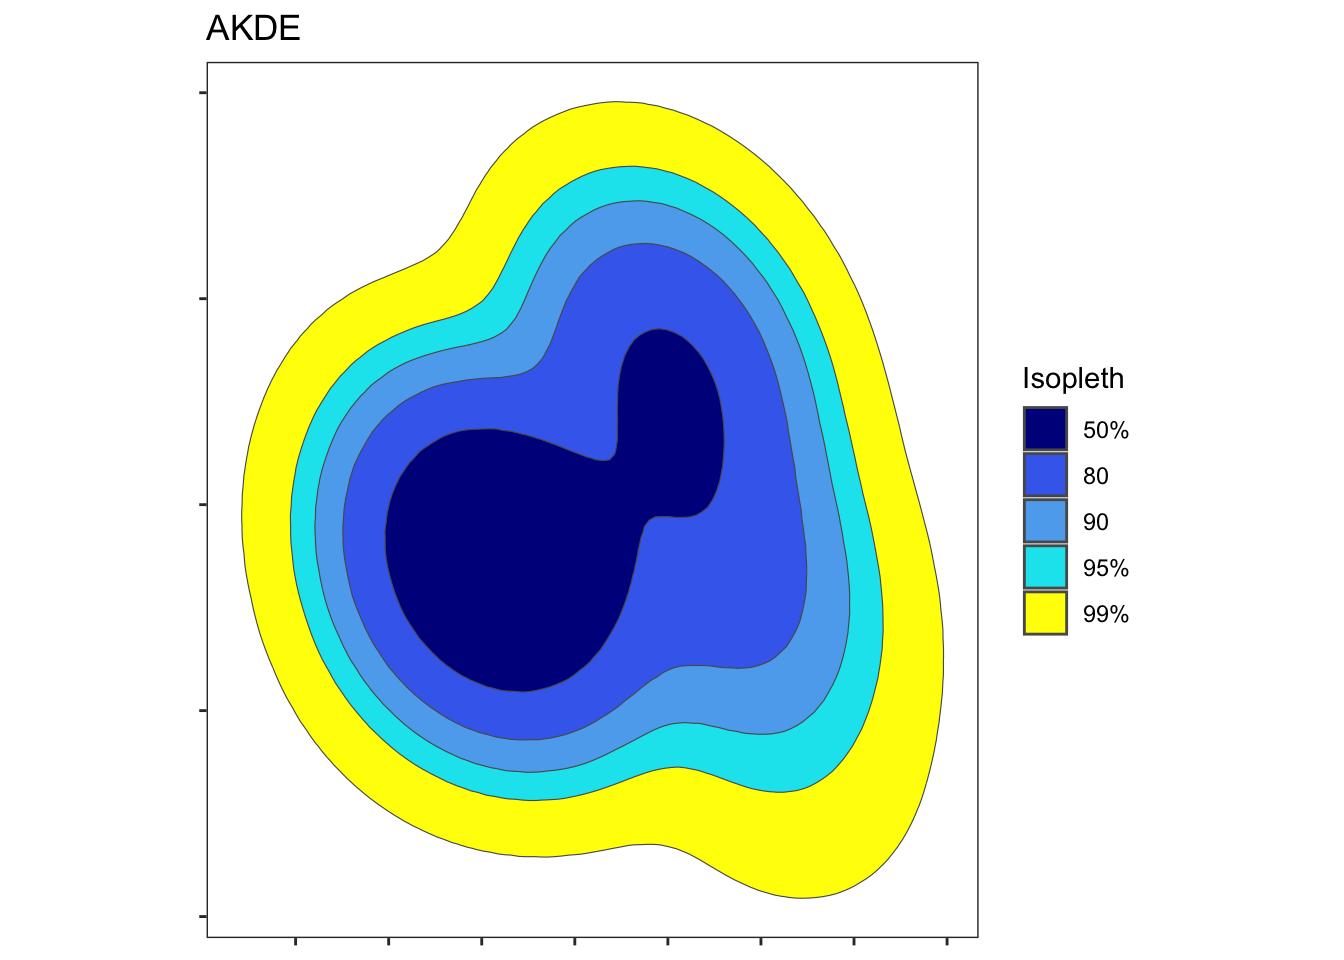
\includegraphics{GridSystem2Script_files/figure-pdf/unnamed-chunk-7-2.pdf}

}

\end{figure}

\begin{enumerate}
\def\labelenumi{\arabic{enumi}.}
\setcounter{enumi}{8}
\tightlist
\item
  Then identify the cell ID that contains each mule deer location from
  the new expanded grid
\end{enumerate}

\begin{Shaded}
\begin{Highlighting}[]
\DocumentationTok{\#\#BE SURE TO RUN CODE FROM XY CREATION THROUGH NEW2 AGAIN THEN LOOK AT DATA!!}
\NormalTok{o2 }\OtherTok{=} \FunctionTok{st\_intersection}\NormalTok{(deer.albers,GridPols2)}
\end{Highlighting}
\end{Shaded}

\begin{verbatim}
Warning: attribute variables are assumed to be spatially constant throughout
all geometries
\end{verbatim}

10. Now we can load a vegetation raster layer using the FedData package
to summarize vegetation categories within each polygon grid cell.

\begin{Shaded}
\begin{Highlighting}[]
\NormalTok{nlcd }\OtherTok{\textless{}{-}} \FunctionTok{get\_nlcd}\NormalTok{(}\AttributeTok{template=}\NormalTok{GridPols2, }\AttributeTok{year =} \DecValTok{2019}\NormalTok{, }\AttributeTok{label =} \StringTok{\textquotesingle{}nlcd\textquotesingle{}}\NormalTok{,}\AttributeTok{force.redo =}\NormalTok{ T)}
\FunctionTok{plot}\NormalTok{(nlcd)}
\end{Highlighting}
\end{Shaded}

\begin{figure}[H]

{\centering 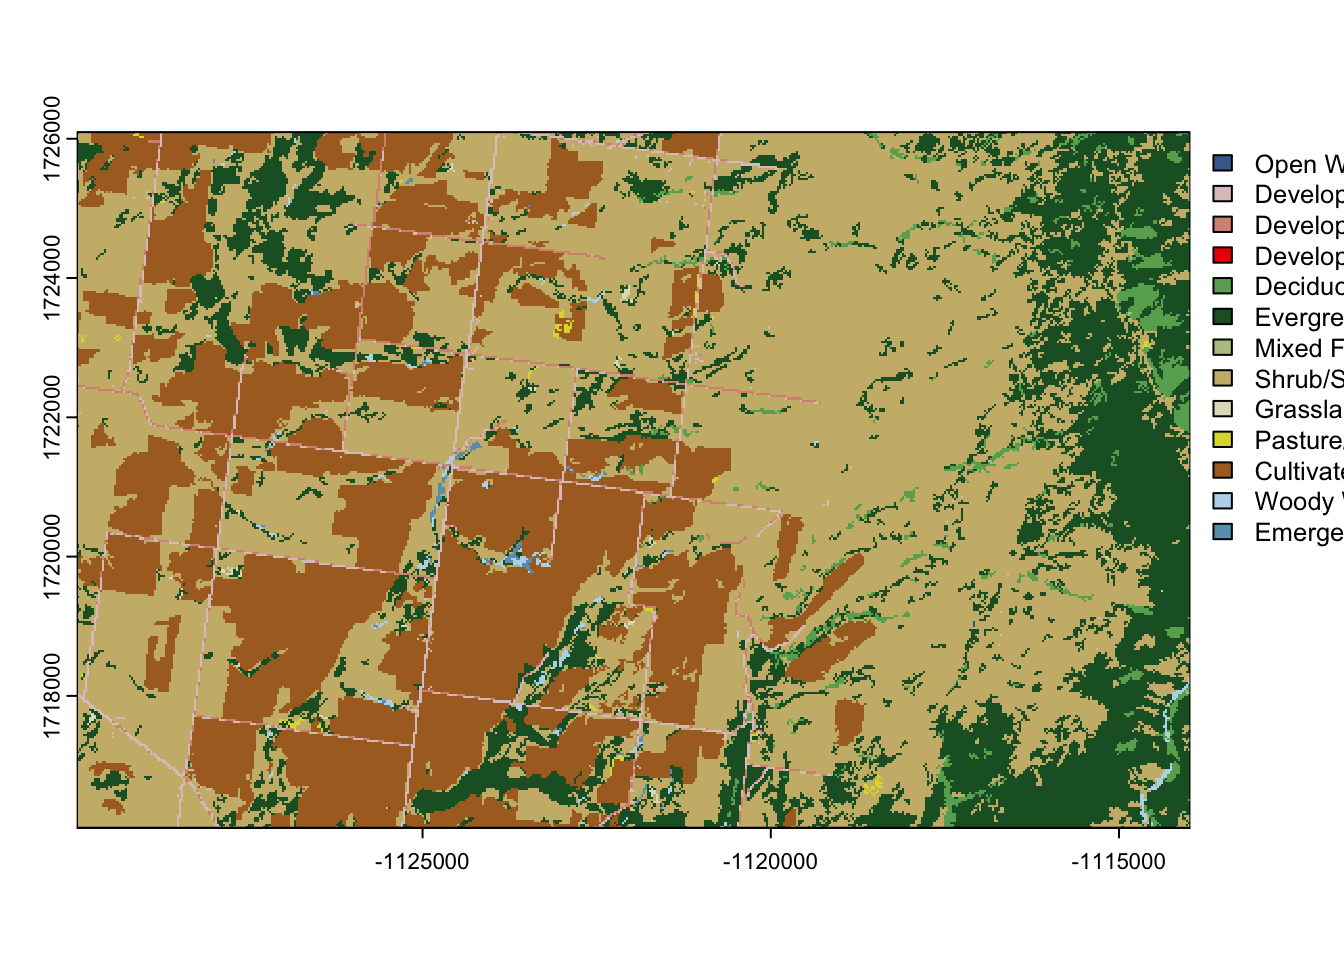
\includegraphics{GridSystem2Script_files/figure-pdf/unnamed-chunk-9-1.pdf}

}

\end{figure}

11. Clip the raster within the extent of the newly created grid

\begin{Shaded}
\begin{Highlighting}[]
\NormalTok{bbclip }\OtherTok{\textless{}{-}} \FunctionTok{crop}\NormalTok{(nlcd, GridPols2)}
\FunctionTok{plot}\NormalTok{(bbclip)}
\FunctionTok{plot}\NormalTok{(}\FunctionTok{st\_geometry}\NormalTok{(deer.albers),}\AttributeTok{add=}\NormalTok{T,}\AttributeTok{col=}\StringTok{"red"}\NormalTok{)}
\FunctionTok{plot}\NormalTok{(}\FunctionTok{st\_geometry}\NormalTok{(GridPols2), }\AttributeTok{add=}\NormalTok{T)}
\end{Highlighting}
\end{Shaded}

\begin{figure}[H]

{\centering 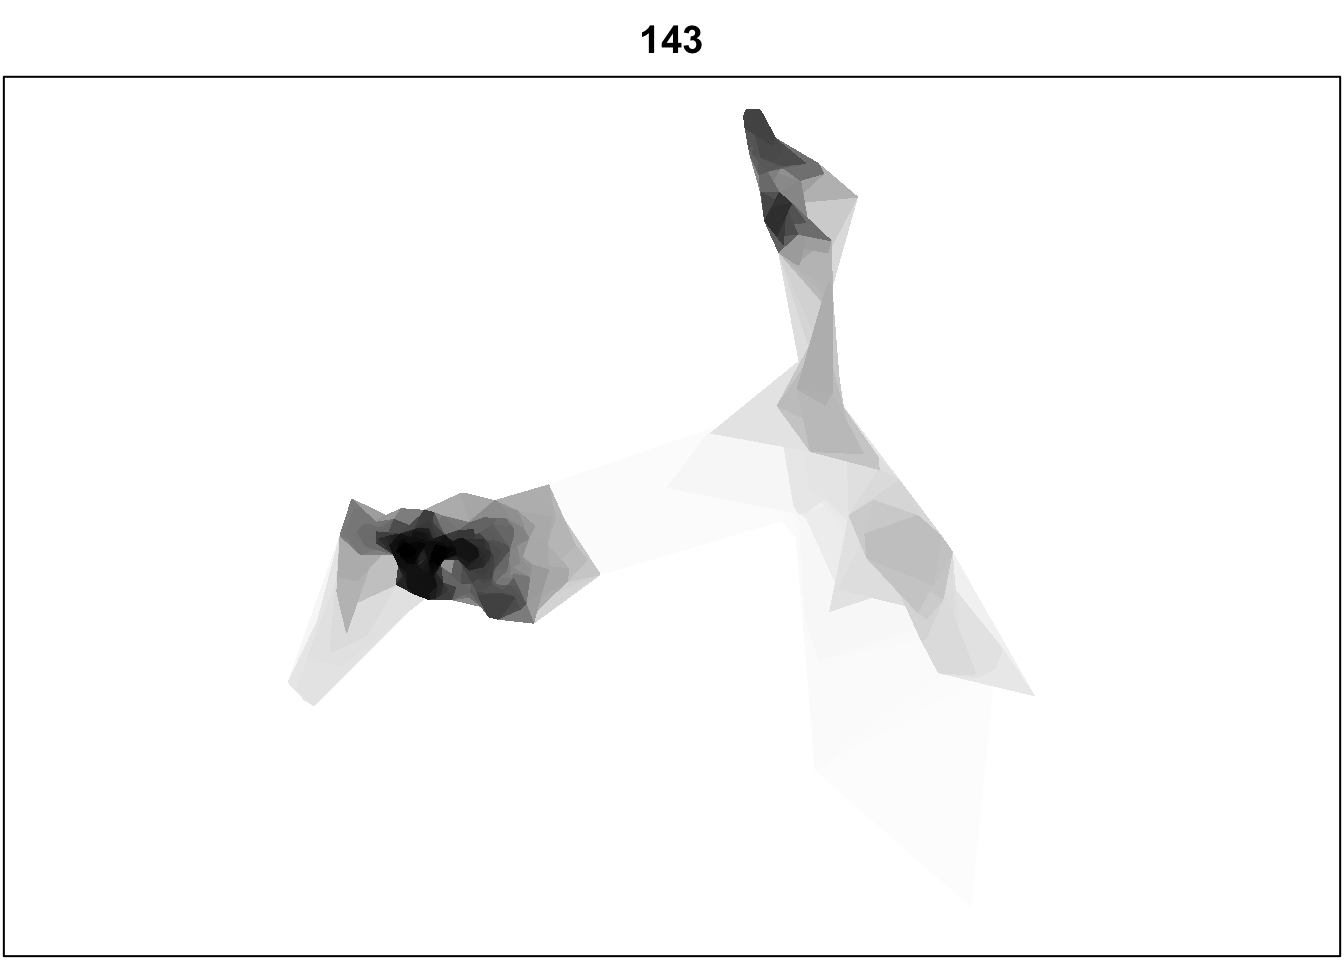
\includegraphics{GridSystem2Script_files/figure-pdf/unnamed-chunk-10-1.pdf}

}

\end{figure}

\begin{Shaded}
\begin{Highlighting}[]
\CommentTok{\#Cell size of raster layer}
\FunctionTok{xres}\NormalTok{(bbclip)}
\end{Highlighting}
\end{Shaded}

\begin{verbatim}
[1] 30
\end{verbatim}

\begin{Shaded}
\begin{Highlighting}[]
\CommentTok{\#Create histogram of vegetation categories in bbclip}
\FunctionTok{hist}\NormalTok{(bbclip)}
\end{Highlighting}
\end{Shaded}

\begin{figure}[H]

{\centering 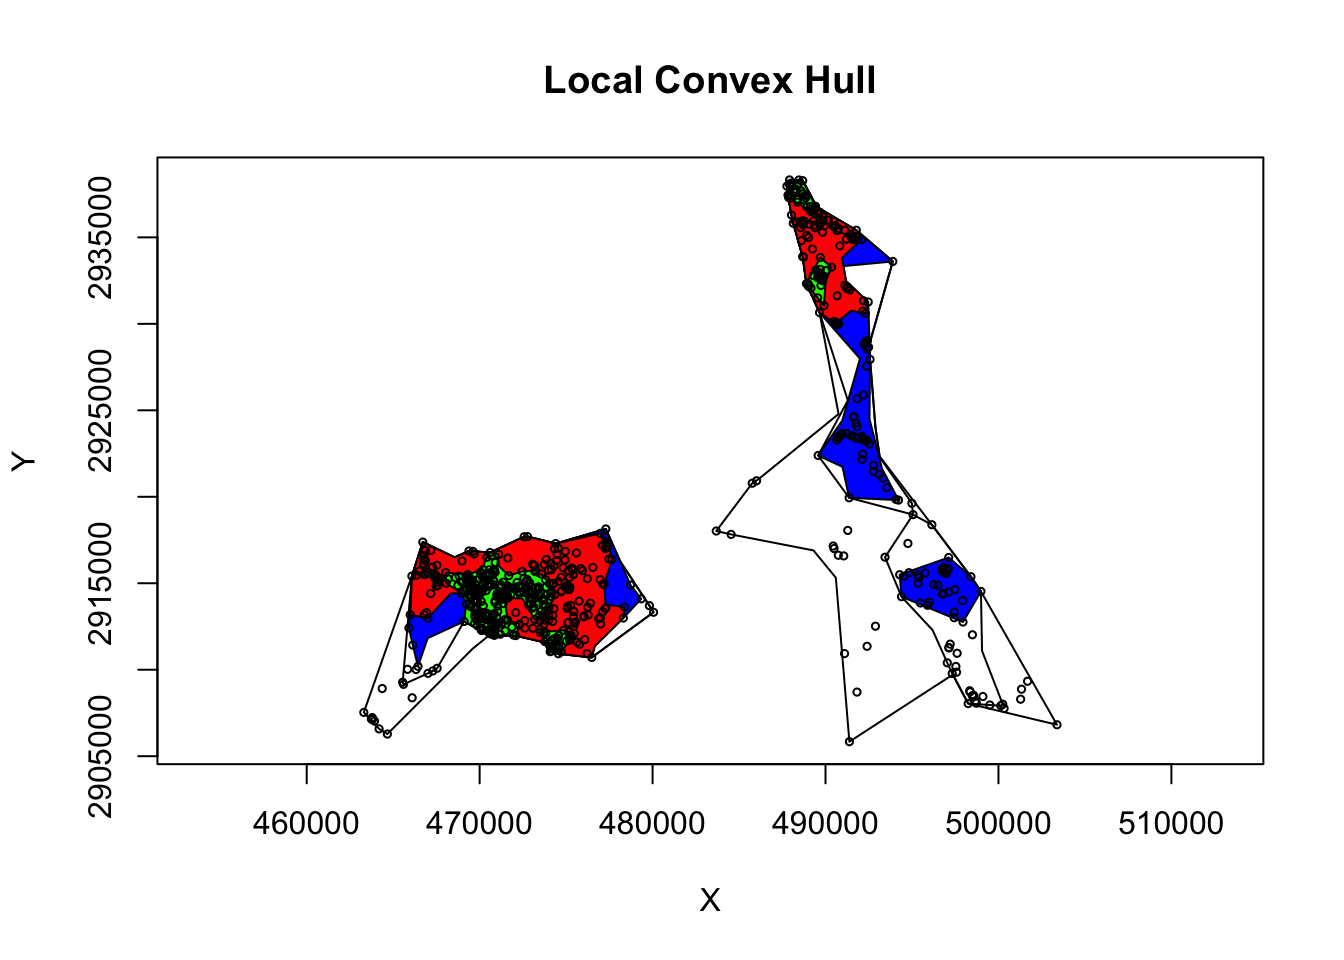
\includegraphics{GridSystem2Script_files/figure-pdf/unnamed-chunk-10-2.pdf}

}

\end{figure}

\begin{Shaded}
\begin{Highlighting}[]
\CommentTok{\#Calculate cell size in square meters}
\NormalTok{ii }\OtherTok{\textless{}{-}} \FunctionTok{st\_area}\NormalTok{(GridPols2)}\CommentTok{\#requires adehabitatMA package}
\NormalTok{ii[}\DecValTok{1}\NormalTok{]}
\end{Highlighting}
\end{Shaded}

\begin{verbatim}
250000 [m^2]
\end{verbatim}

\begin{enumerate}
\def\labelenumi{\arabic{enumi}.}
\setcounter{enumi}{11}
\tightlist
\item
  We can extract the vegetation characteristics within each polygon of
  the grid and then tabulate area of each vegetation category within
  each polygon by extracting vegetation within each polygon by ID then
  summarizing the vegetation characteristics in each cell to be used in
  future resource selection analysis or disease epidemiology.
\end{enumerate}

\begin{Shaded}
\begin{Highlighting}[]
\FunctionTok{library}\NormalTok{(exactextractr)}
\NormalTok{area }\OtherTok{=} \FunctionTok{exact\_extract}\NormalTok{(bbclip,GridPols2)}
\end{Highlighting}
\end{Shaded}

\begin{verbatim}

  |                                                                            
  |                                                                      |   0%
  |                                                                            
  |                                                                      |   1%
  |                                                                            
  |=                                                                     |   1%
  |                                                                            
  |=                                                                     |   2%
  |                                                                            
  |==                                                                    |   2%
  |                                                                            
  |==                                                                    |   3%
  |                                                                            
  |===                                                                   |   4%
  |                                                                            
  |===                                                                   |   5%
  |                                                                            
  |====                                                                  |   5%
  |                                                                            
  |====                                                                  |   6%
  |                                                                            
  |=====                                                                 |   7%
  |                                                                            
  |=====                                                                 |   8%
  |                                                                            
  |======                                                                |   8%
  |                                                                            
  |======                                                                |   9%
  |                                                                            
  |=======                                                               |   9%
  |                                                                            
  |=======                                                               |  10%
  |                                                                            
  |=======                                                               |  11%
  |                                                                            
  |========                                                              |  11%
  |                                                                            
  |========                                                              |  12%
  |                                                                            
  |=========                                                             |  12%
  |                                                                            
  |=========                                                             |  13%
  |                                                                            
  |==========                                                            |  14%
  |                                                                            
  |==========                                                            |  15%
  |                                                                            
  |===========                                                           |  15%
  |                                                                            
  |===========                                                           |  16%
  |                                                                            
  |============                                                          |  17%
  |                                                                            
  |============                                                          |  18%
  |                                                                            
  |=============                                                         |  18%
  |                                                                            
  |=============                                                         |  19%
  |                                                                            
  |==============                                                        |  19%
  |                                                                            
  |==============                                                        |  20%
  |                                                                            
  |==============                                                        |  21%
  |                                                                            
  |===============                                                       |  21%
  |                                                                            
  |===============                                                       |  22%
  |                                                                            
  |================                                                      |  22%
  |                                                                            
  |================                                                      |  23%
  |                                                                            
  |=================                                                     |  24%
  |                                                                            
  |=================                                                     |  25%
  |                                                                            
  |==================                                                    |  25%
  |                                                                            
  |==================                                                    |  26%
  |                                                                            
  |===================                                                   |  27%
  |                                                                            
  |===================                                                   |  28%
  |                                                                            
  |====================                                                  |  28%
  |                                                                            
  |====================                                                  |  29%
  |                                                                            
  |=====================                                                 |  29%
  |                                                                            
  |=====================                                                 |  30%
  |                                                                            
  |=====================                                                 |  31%
  |                                                                            
  |======================                                                |  31%
  |                                                                            
  |======================                                                |  32%
  |                                                                            
  |=======================                                               |  32%
  |                                                                            
  |=======================                                               |  33%
  |                                                                            
  |========================                                              |  34%
  |                                                                            
  |========================                                              |  35%
  |                                                                            
  |=========================                                             |  35%
  |                                                                            
  |=========================                                             |  36%
  |                                                                            
  |==========================                                            |  37%
  |                                                                            
  |==========================                                            |  38%
  |                                                                            
  |===========================                                           |  38%
  |                                                                            
  |===========================                                           |  39%
  |                                                                            
  |============================                                          |  39%
  |                                                                            
  |============================                                          |  40%
  |                                                                            
  |============================                                          |  41%
  |                                                                            
  |=============================                                         |  41%
  |                                                                            
  |=============================                                         |  42%
  |                                                                            
  |==============================                                        |  42%
  |                                                                            
  |==============================                                        |  43%
  |                                                                            
  |===============================                                       |  44%
  |                                                                            
  |===============================                                       |  45%
  |                                                                            
  |================================                                      |  45%
  |                                                                            
  |================================                                      |  46%
  |                                                                            
  |=================================                                     |  47%
  |                                                                            
  |=================================                                     |  48%
  |                                                                            
  |==================================                                    |  48%
  |                                                                            
  |==================================                                    |  49%
  |                                                                            
  |===================================                                   |  49%
  |                                                                            
  |===================================                                   |  50%
  |                                                                            
  |===================================                                   |  51%
  |                                                                            
  |====================================                                  |  51%
  |                                                                            
  |====================================                                  |  52%
  |                                                                            
  |=====================================                                 |  52%
  |                                                                            
  |=====================================                                 |  53%
  |                                                                            
  |======================================                                |  54%
  |                                                                            
  |======================================                                |  55%
  |                                                                            
  |=======================================                               |  55%
  |                                                                            
  |=======================================                               |  56%
  |                                                                            
  |========================================                              |  57%
  |                                                                            
  |========================================                              |  58%
  |                                                                            
  |=========================================                             |  58%
  |                                                                            
  |=========================================                             |  59%
  |                                                                            
  |==========================================                            |  59%
  |                                                                            
  |==========================================                            |  60%
  |                                                                            
  |==========================================                            |  61%
  |                                                                            
  |===========================================                           |  61%
  |                                                                            
  |===========================================                           |  62%
  |                                                                            
  |============================================                          |  62%
  |                                                                            
  |============================================                          |  63%
  |                                                                            
  |=============================================                         |  64%
  |                                                                            
  |=============================================                         |  65%
  |                                                                            
  |==============================================                        |  65%
  |                                                                            
  |==============================================                        |  66%
  |                                                                            
  |===============================================                       |  67%
  |                                                                            
  |===============================================                       |  68%
  |                                                                            
  |================================================                      |  68%
  |                                                                            
  |================================================                      |  69%
  |                                                                            
  |=================================================                     |  69%
  |                                                                            
  |=================================================                     |  70%
  |                                                                            
  |=================================================                     |  71%
  |                                                                            
  |==================================================                    |  71%
  |                                                                            
  |==================================================                    |  72%
  |                                                                            
  |===================================================                   |  72%
  |                                                                            
  |===================================================                   |  73%
  |                                                                            
  |====================================================                  |  74%
  |                                                                            
  |====================================================                  |  75%
  |                                                                            
  |=====================================================                 |  75%
  |                                                                            
  |=====================================================                 |  76%
  |                                                                            
  |======================================================                |  77%
  |                                                                            
  |======================================================                |  78%
  |                                                                            
  |=======================================================               |  78%
  |                                                                            
  |=======================================================               |  79%
  |                                                                            
  |========================================================              |  79%
  |                                                                            
  |========================================================              |  80%
  |                                                                            
  |========================================================              |  81%
  |                                                                            
  |=========================================================             |  81%
  |                                                                            
  |=========================================================             |  82%
  |                                                                            
  |==========================================================            |  82%
  |                                                                            
  |==========================================================            |  83%
  |                                                                            
  |===========================================================           |  84%
  |                                                                            
  |===========================================================           |  85%
  |                                                                            
  |============================================================          |  85%
  |                                                                            
  |============================================================          |  86%
  |                                                                            
  |=============================================================         |  87%
  |                                                                            
  |=============================================================         |  88%
  |                                                                            
  |==============================================================        |  88%
  |                                                                            
  |==============================================================        |  89%
  |                                                                            
  |===============================================================       |  89%
  |                                                                            
  |===============================================================       |  90%
  |                                                                            
  |===============================================================       |  91%
  |                                                                            
  |================================================================      |  91%
  |                                                                            
  |================================================================      |  92%
  |                                                                            
  |=================================================================     |  92%
  |                                                                            
  |=================================================================     |  93%
  |                                                                            
  |==================================================================    |  94%
  |                                                                            
  |==================================================================    |  95%
  |                                                                            
  |===================================================================   |  95%
  |                                                                            
  |===================================================================   |  96%
  |                                                                            
  |====================================================================  |  97%
  |                                                                            
  |====================================================================  |  98%
  |                                                                            
  |===================================================================== |  98%
  |                                                                            
  |===================================================================== |  99%
  |                                                                            
  |======================================================================|  99%
  |                                                                            
  |======================================================================| 100%
\end{verbatim}

\begin{Shaded}
\begin{Highlighting}[]
\NormalTok{classes }\OtherTok{\textless{}{-}} \FunctionTok{sort}\NormalTok{(}\FunctionTok{unique}\NormalTok{(bbclip[]))}
\NormalTok{combine }\OtherTok{\textless{}{-}} \FunctionTok{lapply}\NormalTok{(area, }\AttributeTok{FUN=}\ControlFlowTok{function}\NormalTok{(x) \{ }\FunctionTok{as.data.frame}\NormalTok{(}\FunctionTok{prop.table}\NormalTok{(}\FunctionTok{table}\NormalTok{(}\FunctionTok{factor}\NormalTok{(x[,}\DecValTok{1}\NormalTok{],}
                          \AttributeTok{levels =}\NormalTok{ classes))))\} ) }
\FunctionTok{head}\NormalTok{(combine)}
\end{Highlighting}
\end{Shaded}

\begin{verbatim}
[[1]]
   Var1       Freq
1    11 0.00000000
2    21 0.00000000
3    22 0.00000000
4    23 0.00000000
5    41 0.00000000
6    42 0.00000000
7    43 0.00000000
8    52 0.92733564
9    71 0.00000000
10   81 0.00000000
11   82 0.07266436
12   90 0.00000000
13   95 0.00000000

[[2]]
   Var1       Freq
1    11 0.00000000
2    21 0.00000000
3    22 0.00000000
4    23 0.00000000
5    41 0.00000000
6    42 0.05228758
7    43 0.00000000
8    52 0.83986928
9    71 0.00000000
10   81 0.00000000
11   82 0.10784314
12   90 0.00000000
13   95 0.00000000

[[3]]
   Var1       Freq
1    11 0.00000000
2    21 0.06535948
3    22 0.00000000
4    23 0.00000000
5    41 0.00000000
6    42 0.00000000
7    43 0.00000000
8    52 0.93464052
9    71 0.00000000
10   81 0.00000000
11   82 0.00000000
12   90 0.00000000
13   95 0.00000000

[[4]]
   Var1        Freq
1    11 0.000000000
2    21 0.076124567
3    22 0.024221453
4    23 0.000000000
5    41 0.000000000
6    42 0.013840830
7    43 0.000000000
8    52 0.882352941
9    71 0.000000000
10   81 0.000000000
11   82 0.003460208
12   90 0.000000000
13   95 0.000000000

[[5]]
   Var1        Freq
1    11 0.000000000
2    21 0.026143791
3    22 0.000000000
4    23 0.000000000
5    41 0.000000000
6    42 0.196078431
7    43 0.000000000
8    52 0.549019608
9    71 0.000000000
10   81 0.003267974
11   82 0.225490196
12   90 0.000000000
13   95 0.000000000

[[6]]
   Var1      Freq
1    11 0.0000000
2    21 0.0000000
3    22 0.0000000
4    23 0.0000000
5    41 0.0000000
6    42 0.3986928
7    43 0.0000000
8    52 0.4052288
9    71 0.0000000
10   81 0.0000000
11   82 0.1960784
12   90 0.0000000
13   95 0.0000000
\end{verbatim}

\hypertarget{creating-buffers}{%
\chapter{Creating Buffers}\label{creating-buffers}}

For this exercise, we will again be working with the Colorado mule deer
locations and rasters from earlier sections (1.3, 1.7). Creating buffers
around locations of animals, plots, or some other variable may be
necessary to determine what occurs around the locations. Often times,in
resource selection studies, we may want to generate buffers that can be
considered used habitat within the buffer as opposed to simply counting
only the habitat that the location is found. Lets begin with loading the
proper packages and mule deer locations from previous exercise. Because
we are dealing with the raster layer projected in Albers, we will need
to project our mule deer locations as we did above.

1. Open the script ``BufferScript.Rmd'' and run code directly from the
script

2. First we need to load the packages needed for the exercise

\begin{Shaded}
\begin{Highlighting}[]
\FunctionTok{library}\NormalTok{(sf)}
\FunctionTok{library}\NormalTok{(terra)}
\FunctionTok{library}\NormalTok{(exactextractr)}
\FunctionTok{library}\NormalTok{(FedData)}
\FunctionTok{library}\NormalTok{(zoo)}
\end{Highlighting}
\end{Shaded}

3. Now let's have a separate section of code to include projection
information we will use throughout the exercise. In previous versions,
these lines of code were within each block of code

\begin{Shaded}
\begin{Highlighting}[]
\NormalTok{ll.crs }\OtherTok{\textless{}{-}} \FunctionTok{st\_crs}\NormalTok{(}\DecValTok{4269}\NormalTok{)}
\NormalTok{utm.crs }\OtherTok{\textless{}{-}} \FunctionTok{st\_crs}\NormalTok{(}\DecValTok{9001}\NormalTok{)}
\NormalTok{albers.crs }\OtherTok{\textless{}{-}} \FunctionTok{st\_crs}\NormalTok{(}\DecValTok{5070}\NormalTok{)}
\end{Highlighting}
\end{Shaded}

4. We will import a dataset then subset by a single deer to make
processing time faster

\begin{Shaded}
\begin{Highlighting}[]
\CommentTok{\#Import the location from earlier exercise}
\NormalTok{muleys }\OtherTok{\textless{}{-}}\FunctionTok{read.csv}\NormalTok{(}\StringTok{"data/muleysexample.csv"}\NormalTok{, }\AttributeTok{header=}\NormalTok{T)}

\CommentTok{\#Remove outlier locations}
\NormalTok{coords }\OtherTok{\textless{}{-}} \FunctionTok{st\_as\_sf}\NormalTok{(muleys, }\AttributeTok{coords =} \FunctionTok{c}\NormalTok{(}\StringTok{"Long"}\NormalTok{, }\StringTok{"Lat"}\NormalTok{), }\AttributeTok{crs =}\NormalTok{ ll.crs)}
\FunctionTok{plot}\NormalTok{(}\FunctionTok{st\_geometry}\NormalTok{(coords),}\AttributeTok{axes=}\NormalTok{T)}
\end{Highlighting}
\end{Shaded}

\begin{figure}[H]

{\centering \includegraphics{BufferScript_files/figure-pdf/unnamed-chunk-3-1.pdf}

}

\end{figure}

\begin{Shaded}
\begin{Highlighting}[]
\NormalTok{deer.spdf }\OtherTok{\textless{}{-}} \FunctionTok{st\_crop}\NormalTok{(coords, }\AttributeTok{xmin=}\SpecialCharTok{{-}}\FloatTok{107.0}\NormalTok{,}\AttributeTok{xmax=}\SpecialCharTok{{-}}\FloatTok{110.5}\NormalTok{,}\AttributeTok{ymin=}\FloatTok{37.8}\NormalTok{,}\AttributeTok{ymax=}\FloatTok{39.0}\NormalTok{)}\CommentTok{\#Visually identified based on previous plot}
\FunctionTok{plot}\NormalTok{(}\FunctionTok{st\_geometry}\NormalTok{(deer.spdf),}\AttributeTok{axes=}\NormalTok{T)}
\end{Highlighting}
\end{Shaded}

\begin{figure}[H]

{\centering \includegraphics{BufferScript_files/figure-pdf/unnamed-chunk-3-2.pdf}

}

\end{figure}

\begin{Shaded}
\begin{Highlighting}[]
\CommentTok{\#Project deer.spdf to Albers as in previous exercise}
\NormalTok{deer.albers }\OtherTok{\textless{}{-}}\FunctionTok{st\_transform}\NormalTok{(deer.spdf, }\AttributeTok{crs=}\NormalTok{albers.crs)}
\FunctionTok{plot}\NormalTok{(}\FunctionTok{st\_geometry}\NormalTok{(deer.albers,}\AttributeTok{axes=}\NormalTok{T))}
\end{Highlighting}
\end{Shaded}

\begin{figure}[H]

{\centering \includegraphics{BufferScript_files/figure-pdf/unnamed-chunk-3-3.pdf}

}

\end{figure}

\begin{Shaded}
\begin{Highlighting}[]
\CommentTok{\#Let us subset data so there are fewer locations to work with}
\NormalTok{muley8 }\OtherTok{\textless{}{-}} \FunctionTok{subset}\NormalTok{(deer.albers, id}\SpecialCharTok{==}\StringTok{"D8"}\NormalTok{)}
\end{Highlighting}
\end{Shaded}

5. For mule deer 8 locations, we will create a bounding box.

\begin{Shaded}
\begin{Highlighting}[]
\NormalTok{bb }\OtherTok{\textless{}{-}} \FunctionTok{st\_bbox}\NormalTok{(muley8) }\SpecialCharTok{\%\textgreater{}\%} \FunctionTok{st\_as\_sfc}\NormalTok{()}
\CommentTok{\#bb \textless{}{-} cbind(x=c({-}108.83966,{-}108.83966,{-}108.9834,{-}108.9834, {-}108.83966), }
\CommentTok{\#  y=c(37.8142, 37.86562,37.86562,37.8142,37.8142))}
\FunctionTok{plot}\NormalTok{(}\FunctionTok{st\_geometry}\NormalTok{(bb))}
\FunctionTok{plot}\NormalTok{(}\FunctionTok{st\_geometry}\NormalTok{(deer.albers),}\AttributeTok{col=}\StringTok{"red"}\NormalTok{,}\AttributeTok{add=}\NormalTok{T)}
\end{Highlighting}
\end{Shaded}

\begin{figure}[H]

{\centering \includegraphics{BufferScript_files/figure-pdf/unnamed-chunk-4-1.pdf}

}

\end{figure}

\newline
6. But let us create a new bounding box that encompass mule deer 8
locations but also extends beyond the periphery of the outermost
locations. Then clip the large vegetation raster again so it is within
the newly created bounding box polygon

\begin{Shaded}
\begin{Highlighting}[]
\CommentTok{\# Create vectors of the x and y points using boundary box created around deer locations}
\NormalTok{bb1 }\OtherTok{\textless{}{-}} \FunctionTok{st\_bbox}\NormalTok{(muley8)}
     
\NormalTok{increment }\OtherTok{=} \DecValTok{2000}
\NormalTok{minx}\OtherTok{=}\NormalTok{(}\FunctionTok{min}\NormalTok{(bb1}\SpecialCharTok{$}\NormalTok{xmin)}\SpecialCharTok{{-}}\NormalTok{(increment))}
\NormalTok{maxx}\OtherTok{=}\NormalTok{(}\FunctionTok{max}\NormalTok{(bb1}\SpecialCharTok{$}\NormalTok{xmax)}\SpecialCharTok{+}\NormalTok{(increment))}
\NormalTok{miny}\OtherTok{=}\NormalTok{(}\FunctionTok{min}\NormalTok{(bb1}\SpecialCharTok{$}\NormalTok{ymin)}\SpecialCharTok{{-}}\NormalTok{(increment))}
\NormalTok{maxy}\OtherTok{=}\NormalTok{(}\FunctionTok{max}\NormalTok{(bb1}\SpecialCharTok{$}\NormalTok{ymax)}\SpecialCharTok{+}\NormalTok{(increment))}
  \CommentTok{\# Create vectors of the x and y points using mean size of deer home range of X square kilometers}
\NormalTok{x}\OtherTok{=}\FunctionTok{seq}\NormalTok{(}\AttributeTok{from=}\NormalTok{minx,}\AttributeTok{to=}\NormalTok{maxx,}\AttributeTok{by=}\NormalTok{increment)}
\NormalTok{y}\OtherTok{=}\FunctionTok{seq}\NormalTok{(}\AttributeTok{from=}\NormalTok{miny,}\AttributeTok{to=}\NormalTok{maxy,}\AttributeTok{by=}\NormalTok{increment)}
\CommentTok{\# Create a grid of all pairs of coordinates (as a data.frame) }
\NormalTok{xy}\OtherTok{=}\FunctionTok{expand.grid}\NormalTok{(}\AttributeTok{x=}\NormalTok{x,}\AttributeTok{y=}\NormalTok{y)}
\NormalTok{grid.pts}\OtherTok{\textless{}{-}}\FunctionTok{st\_as\_sf}\NormalTok{(xy, }\AttributeTok{coords =} \FunctionTok{c}\NormalTok{(}\StringTok{"x"}\NormalTok{,}\StringTok{"y"}\NormalTok{),}\AttributeTok{crs =}\NormalTok{ albers.crs)}
\FunctionTok{plot}\NormalTok{(}\FunctionTok{st\_geometry}\NormalTok{(grid.pts))}
\end{Highlighting}
\end{Shaded}

\begin{figure}[H]

{\centering \includegraphics{BufferScript_files/figure-pdf/unnamed-chunk-5-1.pdf}

}

\end{figure}

\begin{Shaded}
\begin{Highlighting}[]
\NormalTok{grid\_spacing }\OtherTok{\textless{}{-}} \DecValTok{500}
\NormalTok{grid }\OtherTok{\textless{}{-}} \FunctionTok{st\_make\_grid}\NormalTok{(grid.pts, }\AttributeTok{square=}\NormalTok{T,}\AttributeTok{cellsize =}\NormalTok{ grid\_spacing) }\SpecialCharTok{\%\textgreater{}\%}
   \FunctionTok{cbind}\NormalTok{(}\FunctionTok{data.frame}\NormalTok{(}\AttributeTok{ID =} \FunctionTok{sprintf}\NormalTok{(}\FunctionTok{paste}\NormalTok{(}\StringTok{"GID\%0"}\NormalTok{,}\FunctionTok{nchar}\NormalTok{(}\FunctionTok{length}\NormalTok{(.)),}\StringTok{"d"}\NormalTok{,}\AttributeTok{sep=}\StringTok{""}\NormalTok{), }\DecValTok{1}\SpecialCharTok{:}\FunctionTok{length}\NormalTok{(.)))) }\SpecialCharTok{\%\textgreater{}\%}
   \FunctionTok{st\_sf}\NormalTok{()}

\FunctionTok{plot}\NormalTok{(}\FunctionTok{st\_geometry}\NormalTok{(grid))}
\FunctionTok{plot}\NormalTok{(}\FunctionTok{st\_geometry}\NormalTok{(muley8),}\AttributeTok{add=}\NormalTok{T, }\AttributeTok{col=}\StringTok{"blue"}\NormalTok{)}
\end{Highlighting}
\end{Shaded}

\begin{figure}[H]

{\centering \includegraphics{BufferScript_files/figure-pdf/unnamed-chunk-5-2.pdf}

}

\end{figure}

7. Now we can load use FedData package with new bounding box to get Land
Cover categories for use later.

\begin{Shaded}
\begin{Highlighting}[]
\NormalTok{nlcd }\OtherTok{\textless{}{-}} \FunctionTok{get\_nlcd}\NormalTok{(}\AttributeTok{template=}\NormalTok{grid, }\AttributeTok{year =} \DecValTok{2019}\NormalTok{, }\AttributeTok{label =} \StringTok{\textquotesingle{}nlcd\textquotesingle{}}\NormalTok{,}\AttributeTok{force.redo =}\NormalTok{ T)}
\FunctionTok{plot}\NormalTok{(nlcd)}
\end{Highlighting}
\end{Shaded}

\begin{figure}[H]

{\centering \includegraphics{BufferScript_files/figure-pdf/unnamed-chunk-6-1.pdf}

}

\end{figure}

8. To conduct some analyses, let us create 100 m buffered circles around
all the locations and extract Land Cover that occurs in each buffered
circle. Most efforts will want percent habitat or area of each habitat
defined individually for each location (i.e., within each buffered
circle).

\begin{Shaded}
\begin{Highlighting}[]
\NormalTok{settbuff}\OtherTok{=}\FunctionTok{st\_buffer}\NormalTok{(muley8,}\DecValTok{500}\NormalTok{) }\SpecialCharTok{\%\textgreater{}\%} \FunctionTok{st\_as\_sfc}\NormalTok{()}
\FunctionTok{plot}\NormalTok{(nlcd)}
\FunctionTok{plot}\NormalTok{(}\FunctionTok{st\_geometry}\NormalTok{(settbuff), }\AttributeTok{add=}\NormalTok{T, }\AttributeTok{lty=}\DecValTok{2}\NormalTok{)}
\end{Highlighting}
\end{Shaded}

\begin{figure}[H]

{\centering \includegraphics{BufferScript_files/figure-pdf/unnamed-chunk-7-1.pdf}

}

\end{figure}

\begin{Shaded}
\begin{Highlighting}[]
\NormalTok{ext }\OtherTok{\textless{}{-}} \FunctionTok{exact\_extract}\NormalTok{(nlcd, }\FunctionTok{st\_as\_sf}\NormalTok{(settbuff))}
\end{Highlighting}
\end{Shaded}

\begin{verbatim}

  |                                                                            
  |                                                                      |   0%
  |                                                                            
  |                                                                      |   1%
  |                                                                            
  |=                                                                     |   1%
  |                                                                            
  |=                                                                     |   2%
  |                                                                            
  |==                                                                    |   2%
  |                                                                            
  |==                                                                    |   3%
  |                                                                            
  |==                                                                    |   4%
  |                                                                            
  |===                                                                   |   4%
  |                                                                            
  |===                                                                   |   5%
  |                                                                            
  |====                                                                  |   5%
  |                                                                            
  |====                                                                  |   6%
  |                                                                            
  |=====                                                                 |   7%
  |                                                                            
  |=====                                                                 |   8%
  |                                                                            
  |======                                                                |   8%
  |                                                                            
  |======                                                                |   9%
  |                                                                            
  |=======                                                               |   9%
  |                                                                            
  |=======                                                               |  10%
  |                                                                            
  |=======                                                               |  11%
  |                                                                            
  |========                                                              |  11%
  |                                                                            
  |========                                                              |  12%
  |                                                                            
  |=========                                                             |  12%
  |                                                                            
  |=========                                                             |  13%
  |                                                                            
  |=========                                                             |  14%
  |                                                                            
  |==========                                                            |  14%
  |                                                                            
  |==========                                                            |  15%
  |                                                                            
  |===========                                                           |  15%
  |                                                                            
  |===========                                                           |  16%
  |                                                                            
  |============                                                          |  17%
  |                                                                            
  |============                                                          |  18%
  |                                                                            
  |=============                                                         |  18%
  |                                                                            
  |=============                                                         |  19%
  |                                                                            
  |==============                                                        |  19%
  |                                                                            
  |==============                                                        |  20%
  |                                                                            
  |==============                                                        |  21%
  |                                                                            
  |===============                                                       |  21%
  |                                                                            
  |===============                                                       |  22%
  |                                                                            
  |================                                                      |  22%
  |                                                                            
  |================                                                      |  23%
  |                                                                            
  |================                                                      |  24%
  |                                                                            
  |=================                                                     |  24%
  |                                                                            
  |=================                                                     |  25%
  |                                                                            
  |==================                                                    |  25%
  |                                                                            
  |==================                                                    |  26%
  |                                                                            
  |===================                                                   |  26%
  |                                                                            
  |===================                                                   |  27%
  |                                                                            
  |===================                                                   |  28%
  |                                                                            
  |====================                                                  |  28%
  |                                                                            
  |====================                                                  |  29%
  |                                                                            
  |=====================                                                 |  29%
  |                                                                            
  |=====================                                                 |  30%
  |                                                                            
  |=====================                                                 |  31%
  |                                                                            
  |======================                                                |  31%
  |                                                                            
  |======================                                                |  32%
  |                                                                            
  |=======================                                               |  32%
  |                                                                            
  |=======================                                               |  33%
  |                                                                            
  |========================                                              |  34%
  |                                                                            
  |========================                                              |  35%
  |                                                                            
  |=========================                                             |  35%
  |                                                                            
  |=========================                                             |  36%
  |                                                                            
  |==========================                                            |  36%
  |                                                                            
  |==========================                                            |  37%
  |                                                                            
  |==========================                                            |  38%
  |                                                                            
  |===========================                                           |  38%
  |                                                                            
  |===========================                                           |  39%
  |                                                                            
  |============================                                          |  39%
  |                                                                            
  |============================                                          |  40%
  |                                                                            
  |============================                                          |  41%
  |                                                                            
  |=============================                                         |  41%
  |                                                                            
  |=============================                                         |  42%
  |                                                                            
  |==============================                                        |  42%
  |                                                                            
  |==============================                                        |  43%
  |                                                                            
  |===============================                                       |  44%
  |                                                                            
  |===============================                                       |  45%
  |                                                                            
  |================================                                      |  45%
  |                                                                            
  |================================                                      |  46%
  |                                                                            
  |=================================                                     |  46%
  |                                                                            
  |=================================                                     |  47%
  |                                                                            
  |=================================                                     |  48%
  |                                                                            
  |==================================                                    |  48%
  |                                                                            
  |==================================                                    |  49%
  |                                                                            
  |===================================                                   |  49%
  |                                                                            
  |===================================                                   |  50%
  |                                                                            
  |===================================                                   |  51%
  |                                                                            
  |====================================                                  |  51%
  |                                                                            
  |====================================                                  |  52%
  |                                                                            
  |=====================================                                 |  52%
  |                                                                            
  |=====================================                                 |  53%
  |                                                                            
  |=====================================                                 |  54%
  |                                                                            
  |======================================                                |  54%
  |                                                                            
  |======================================                                |  55%
  |                                                                            
  |=======================================                               |  55%
  |                                                                            
  |=======================================                               |  56%
  |                                                                            
  |========================================                              |  57%
  |                                                                            
  |========================================                              |  58%
  |                                                                            
  |=========================================                             |  58%
  |                                                                            
  |=========================================                             |  59%
  |                                                                            
  |==========================================                            |  59%
  |                                                                            
  |==========================================                            |  60%
  |                                                                            
  |==========================================                            |  61%
  |                                                                            
  |===========================================                           |  61%
  |                                                                            
  |===========================================                           |  62%
  |                                                                            
  |============================================                          |  62%
  |                                                                            
  |============================================                          |  63%
  |                                                                            
  |============================================                          |  64%
  |                                                                            
  |=============================================                         |  64%
  |                                                                            
  |=============================================                         |  65%
  |                                                                            
  |==============================================                        |  65%
  |                                                                            
  |==============================================                        |  66%
  |                                                                            
  |===============================================                       |  67%
  |                                                                            
  |===============================================                       |  68%
  |                                                                            
  |================================================                      |  68%
  |                                                                            
  |================================================                      |  69%
  |                                                                            
  |=================================================                     |  69%
  |                                                                            
  |=================================================                     |  70%
  |                                                                            
  |=================================================                     |  71%
  |                                                                            
  |==================================================                    |  71%
  |                                                                            
  |==================================================                    |  72%
  |                                                                            
  |===================================================                   |  72%
  |                                                                            
  |===================================================                   |  73%
  |                                                                            
  |===================================================                   |  74%
  |                                                                            
  |====================================================                  |  74%
  |                                                                            
  |====================================================                  |  75%
  |                                                                            
  |=====================================================                 |  75%
  |                                                                            
  |=====================================================                 |  76%
  |                                                                            
  |======================================================                |  76%
  |                                                                            
  |======================================================                |  77%
  |                                                                            
  |======================================================                |  78%
  |                                                                            
  |=======================================================               |  78%
  |                                                                            
  |=======================================================               |  79%
  |                                                                            
  |========================================================              |  79%
  |                                                                            
  |========================================================              |  80%
  |                                                                            
  |========================================================              |  81%
  |                                                                            
  |=========================================================             |  81%
  |                                                                            
  |=========================================================             |  82%
  |                                                                            
  |==========================================================            |  82%
  |                                                                            
  |==========================================================            |  83%
  |                                                                            
  |===========================================================           |  84%
  |                                                                            
  |===========================================================           |  85%
  |                                                                            
  |============================================================          |  85%
  |                                                                            
  |============================================================          |  86%
  |                                                                            
  |=============================================================         |  86%
  |                                                                            
  |=============================================================         |  87%
  |                                                                            
  |=============================================================         |  88%
  |                                                                            
  |==============================================================        |  88%
  |                                                                            
  |==============================================================        |  89%
  |                                                                            
  |===============================================================       |  89%
  |                                                                            
  |===============================================================       |  90%
  |                                                                            
  |===============================================================       |  91%
  |                                                                            
  |================================================================      |  91%
  |                                                                            
  |================================================================      |  92%
  |                                                                            
  |=================================================================     |  92%
  |                                                                            
  |=================================================================     |  93%
  |                                                                            
  |==================================================================    |  94%
  |                                                                            
  |==================================================================    |  95%
  |                                                                            
  |===================================================================   |  95%
  |                                                                            
  |===================================================================   |  96%
  |                                                                            
  |====================================================================  |  96%
  |                                                                            
  |====================================================================  |  97%
  |                                                                            
  |====================================================================  |  98%
  |                                                                            
  |===================================================================== |  98%
  |                                                                            
  |===================================================================== |  99%
  |                                                                            
  |======================================================================|  99%
  |                                                                            
  |======================================================================| 100%
\end{verbatim}

\begin{Shaded}
\begin{Highlighting}[]
\FunctionTok{head}\NormalTok{(ext[[}\DecValTok{1}\NormalTok{]])}\CommentTok{\#Here we can see the percent of each category in buffer IDs 1{-}6 for category 52}
\end{Highlighting}
\end{Shaded}

\begin{verbatim}
  value coverage_fraction
1    52       0.006735825
2    52       0.170379668
3    52       0.352209508
4    52       0.472016335
5    52       0.531102777
6    52       0.529586434
\end{verbatim}

\begin{Shaded}
\begin{Highlighting}[]
\NormalTok{et}\OtherTok{=}\FunctionTok{lapply}\NormalTok{(ext,table)}

\NormalTok{prop }\OtherTok{\textless{}{-}} \FunctionTok{list}\NormalTok{()}
\ControlFlowTok{for}\NormalTok{(i }\ControlFlowTok{in} \DecValTok{1}\SpecialCharTok{:}\FunctionTok{length}\NormalTok{(ext)[}\DecValTok{1}\NormalTok{] )\{}
\NormalTok{  prop[[i]] }\OtherTok{\textless{}{-}} \FunctionTok{round}\NormalTok{((}\FunctionTok{margin.table}\NormalTok{(et[[i]],}\DecValTok{1}\NormalTok{)}\SpecialCharTok{/}\FunctionTok{margin.table}\NormalTok{(et[[i]])),}\AttributeTok{digits =} \DecValTok{6}\NormalTok{)}
\NormalTok{\}}
\NormalTok{prop}
\end{Highlighting}
\end{Shaded}

\begin{verbatim}
[[1]]
value
      41       42       52       82 
0.061637 0.058448 0.602550 0.277365 

[[2]]
value
      41       42       52 
0.014878 0.020191 0.964931 

[[3]]
value
      41       42       52 
0.032979 0.075532 0.891489 

[[4]]
value
      21       41       42       52 
0.002130 0.047923 0.102236 0.847710 

[[5]]
value
      41       42       52 
0.067308 0.198718 0.733974 

[[6]]
value
      21       22       41       42       52       82 
0.004255 0.028723 0.043617 0.050000 0.714894 0.158511 

[[7]]
value
      21       22       41       42       52       82 
0.005319 0.028723 0.043617 0.050000 0.714894 0.157447 

[[8]]
value
      21       41       42       52       82 
0.008493 0.049894 0.070064 0.604034 0.267516 

[[9]]
value
      21       41       42       52       82 
0.008493 0.049894 0.070064 0.604034 0.267516 

[[10]]
value
      21       41       42       52       82 
0.008502 0.049947 0.070138 0.603613 0.267800 

[[11]]
value
      21       41       42       52       82 
0.006403 0.050160 0.071505 0.606190 0.265742 

[[12]]
value
      21       41       42       52       82 
0.004251 0.046759 0.069075 0.612115 0.267800 

[[13]]
value
      21       41       42       52       82 
0.004269 0.045891 0.068303 0.614728 0.266809 

[[14]]
value
      21       41       42       52       82 
0.004269 0.045891 0.068303 0.612593 0.268943 

[[15]]
value
      21       41       42       52       82 
0.003185 0.046709 0.069002 0.613588 0.267516 

[[16]]
value
      41       42       52       82 
0.056144 0.063559 0.618644 0.261653 

[[17]]
value
      41       42       52       82 
0.059574 0.059574 0.595745 0.285106 

[[18]]
value
      21       41       42       52       82 
0.002139 0.049198 0.064171 0.621390 0.263102 

[[19]]
value
      21       41       42       52       82 
0.006383 0.047872 0.071277 0.604255 0.270213 

[[20]]
value
      21       41       42       52       82 
0.004255 0.045745 0.069149 0.611702 0.269149 

[[21]]
value
      21       41       42       52       82 
0.004255 0.046809 0.068085 0.612766 0.268085 

[[22]]
value
      21       41       42       52       82 
0.002121 0.048780 0.066808 0.620361 0.261930 

[[23]]
value
      21       22       41       42       52       82 
0.004260 0.027689 0.031949 0.041534 0.747604 0.146965 

[[24]]
value
      21       22       41       42       52       82 
0.004255 0.027660 0.032979 0.041489 0.743617 0.150000 

[[25]]
value
      21       41       42       52       82 
0.017021 0.054255 0.060638 0.630851 0.237234 

[[26]]
value
      21       22       41       42       52       82 
0.025424 0.016949 0.044492 0.056144 0.634534 0.222458 

[[27]]
value
      21       22       41       42       52       82 
0.014862 0.010616 0.044586 0.058386 0.647558 0.223992 

[[28]]
value
      21       22       41       42       52       82 
0.012766 0.006383 0.044681 0.059574 0.652128 0.224468 

[[29]]
value
      21       22       41       42       52       82 
0.012752 0.006376 0.044633 0.059511 0.654623 0.222104 

[[30]]
value
      21       22       41       42       52       82 
0.012793 0.008529 0.044776 0.058635 0.659915 0.215352 

[[31]]
value
      21       22       41       42       52       82 
0.002125 0.009564 0.020191 0.030818 0.756642 0.180659 

[[32]]
value
      22       41       42       52       82 
0.004255 0.045745 0.064894 0.762766 0.122340 

[[33]]
value
      21       22       41       42       52       82 
0.004269 0.026681 0.008538 0.029883 0.687300 0.243330 

[[34]]
value
      22       41       42       52       82 
0.008538 0.042689 0.048026 0.770544 0.130203 

[[35]]
value
      21       41       42       52       82 
0.004255 0.046809 0.069149 0.612766 0.267021 

[[36]]
value
      21       41       42       52       82 
0.004274 0.045940 0.068376 0.611111 0.270299 

[[37]]
value
      21       41       42       52       82 
0.004251 0.046759 0.071201 0.609989 0.267800 

[[38]]
value
      21       41       42       52       82 
0.004283 0.046039 0.068522 0.612420 0.268737 

[[39]]
value
      21       22       41       42       52       82 
0.004264 0.027719 0.024520 0.038380 0.732409 0.172708 

[[40]]
value
      21       22       41       42       52       82 
0.013800 0.031847 0.043524 0.049894 0.676221 0.184713 

[[41]]
value
      21       22       41       42       52       82 
0.035294 0.022460 0.044920 0.058824 0.638503 0.200000 

[[42]]
value
      21       22       41       42       52       82 
0.042463 0.023355 0.041401 0.063694 0.639066 0.190021 

[[43]]
value
      21       41       42       52       82 
0.011740 0.046958 0.059765 0.649947 0.231590 

[[44]]
value
      21       41       42       52       82 
0.011727 0.046908 0.059701 0.650320 0.231343 

[[45]]
value
      21       41       42       52       82 
0.011702 0.046809 0.059574 0.646809 0.235106 

[[46]]
value
      21       41       42       52       82 
0.011715 0.046858 0.060703 0.647497 0.233227 

[[47]]
value
      21       22       41       42       52       82 
0.004269 0.027748 0.020277 0.037353 0.715048 0.195304 

[[48]]
value
      21       22       41       42       52       82 
0.004251 0.026567 0.015940 0.034006 0.705632 0.213603 

[[49]]
value
      21       22       41       42       52       82 
0.004242 0.027572 0.033934 0.041357 0.743372 0.149523 

[[50]]
value
      21       22       41       42       52       82 
0.004246 0.026539 0.033970 0.041401 0.746285 0.147558 

[[51]]
value
      21       22       41       42       52       82 
0.004233 0.025397 0.044444 0.052910 0.710053 0.162963 

[[52]]
value
      21       22       41       42       52       82 
0.005336 0.029883 0.043757 0.050160 0.713981 0.156884 

[[53]]
value
      21       22       41       42       52       82 
0.005342 0.029915 0.043803 0.050214 0.714744 0.155983 

[[54]]
value
      21       22       41       42       52       82 
0.005308 0.028662 0.043524 0.049894 0.714437 0.158174 

[[55]]
value
      21       41       42       52       82 
0.021322 0.063966 0.065032 0.615139 0.234542 

[[56]]
value
      21       41       42       52       82 
0.016949 0.059322 0.064619 0.617585 0.241525 

[[57]]
value
      41       42       52       82 
0.056503 0.062900 0.626866 0.253731 

[[58]]
value
      21       41       42       52       82 
0.004260 0.045793 0.069223 0.612354 0.268371 

[[59]]
value
      21       41       42       52       82 
0.008466 0.049735 0.068783 0.607407 0.265608 

[[60]]
value
      21       41       42       52       82 
0.007431 0.049894 0.069002 0.608280 0.265393 

[[61]]
value
      21       41       42       52       82 
0.007455 0.050053 0.070288 0.608094 0.264111 

[[62]]
value
      21       41       42       52       82 
0.006403 0.049093 0.072572 0.605123 0.266809 

[[63]]
value
      21       22       42       52       82 
0.002132 0.021322 0.025586 0.656716 0.294243 

[[64]]
value
      21       22       41       42       52       82 
0.001065 0.008520 0.011715 0.027689 0.732694 0.218317 

[[65]]
value
      21       22       41       42       52       82 
0.002134 0.010672 0.036286 0.040555 0.767343 0.143010 

[[66]]
value
      22       41       42       52       82 
0.004260 0.045793 0.062833 0.764643 0.122471 

[[67]]
value
      21       41       42       52       82 
0.004255 0.046809 0.070213 0.610638 0.268085 

[[68]]
value
      21       41       42       52       82 
0.004269 0.045891 0.068303 0.612593 0.268943 

[[69]]
value
      21       41       42       52       82 
0.004255 0.045745 0.069149 0.612766 0.268085 

[[70]]
value
      21       41       42       52       82 
0.004269 0.045891 0.068303 0.612593 0.268943 

[[71]]
value
      21       22       41       42       52       82 
0.004260 0.027689 0.020234 0.037274 0.715655 0.194888 

[[72]]
value
      21       22       41       42       52       82 
0.004274 0.025641 0.006410 0.027778 0.675214 0.260684 

[[73]]
value
      21       22       41       42       52       82 
0.001063 0.008502 0.040383 0.041445 0.769394 0.139214 

[[74]]
value
      21       22       41       42       52       90 
0.038217 0.022293 0.008493 0.233546 0.695329 0.002123 

[[75]]
value
      21       41       42       52       82 
0.004251 0.052072 0.072264 0.616366 0.255048 

[[76]]
value
      21       41       42       52       82 
0.004269 0.045891 0.068303 0.612593 0.268943 

[[77]]
value
      21       41       42       52       82 
0.004274 0.045940 0.068376 0.613248 0.268162 

[[78]]
value
      41       42       52       82 
0.048832 0.078556 0.633758 0.238854 

[[79]]
value
      41       42       52       82 
0.028693 0.089267 0.879915 0.002125 

[[80]]
value
      21       41       42       52       82 
0.004260 0.031949 0.071353 0.864750 0.027689 

[[81]]
value
      21       41       42       52       82 
0.004251 0.035069 0.040383 0.912859 0.007439 

[[82]]
value
      41       42       52 
0.025451 0.009544 0.965005 

[[83]]
value
      41       42       52 
0.025451 0.003181 0.971368 

[[84]]
value
      41       42       52 
0.037116 0.069989 0.892895 

[[85]]
value
      41       42       52 
0.025641 0.043803 0.930556 

[[86]]
value
      41       42       52 
0.026483 0.049788 0.923729 

[[87]]
value
      21       41       42       52       82 
0.004274 0.040598 0.035256 0.898504 0.021368 

[[88]]
value
      21       41       42       52       82 
0.004264 0.040512 0.035181 0.898721 0.021322 

[[89]]
value
      21       41       42       52       82 
0.004260 0.040469 0.035144 0.898829 0.021299 

[[90]]
value
      21       22       41       42       52       82 
0.016985 0.005308 0.010616 0.011677 0.715499 0.239915 

[[91]]
value
      41       42       52 
0.041401 0.063694 0.894904 

[[92]]
value
      41       42       52 
0.041622 0.058698 0.899680 

[[93]]
value
      41       42       52 
0.041489 0.059574 0.898936 

[[94]]
value
      41       42       52 
0.042599 0.059638 0.897764 

[[95]]
value
      41       42       52 
0.040297 0.081654 0.878049 

[[96]]
value
      41       52 
0.013889 0.986111 

[[97]]
value
      42       52 
0.007447 0.992553 

[[98]]
value
      41       42       52 
0.031847 0.043524 0.924628 

[[99]]
value
      41       42       52 
0.043571 0.051010 0.905420 

[[100]]
value
      41       42       52 
0.025451 0.046660 0.927890 

[[101]]
value
      41       42       52 
0.025397 0.046561 0.928042 

[[102]]
value
      41       42       52 
0.025641 0.048077 0.926282 

[[103]]
value
      21       41       42       52       82 
0.004233 0.041270 0.058201 0.853968 0.042328 

[[104]]
value
      21       41       42       52       82 
0.004264 0.041578 0.059701 0.857143 0.037313 

[[105]]
value
      41       42       52       82 
0.032874 0.089077 0.820785 0.057264 

[[106]]
value
      41       42       52       82 
0.024442 0.058448 0.718385 0.198725 

[[107]]
value
      21       22       41       42       52       82       90 
0.051010 0.024442 0.046759 0.279490 0.460149 0.134963 0.003188 

[[108]]
value
      21       22       41       42       52       82       90 
0.051173 0.025586 0.040512 0.278252 0.490405 0.110874 0.003198 

[[109]]
value
      21       22       41       42       52       82       90 
0.052239 0.024520 0.044776 0.281450 0.466951 0.126866 0.003198 

[[110]]
value
      21       22       41       42       52       82       90 
0.050107 0.026652 0.050107 0.266525 0.466951 0.136461 0.003198 

[[111]]
value
      21       22       41       42       52       82       90 
0.044728 0.033014 0.022364 0.152290 0.593184 0.151225 0.003195 

[[112]]
value
      21       22       41       42       52       82       90 
0.047821 0.034006 0.026567 0.158342 0.580234 0.149841 0.003188 

[[113]]
value
      21       22       41       42       52       82       90 
0.045503 0.033862 0.025397 0.129101 0.607407 0.155556 0.003175 

[[114]]
value
      21       22       41       42       52       82 
0.041357 0.023330 0.040297 0.061506 0.639449 0.194062 

[[115]]
value
      21       41       42       52       82 
0.007447 0.050000 0.070213 0.607447 0.264894 

[[116]]
value
      21       41       42       52       82 
0.006390 0.050053 0.071353 0.607029 0.265176 

[[117]]
value
      21       41       42       52       82 
0.007447 0.050000 0.069149 0.607447 0.265957 

[[118]]
value
      21       41       42       52       82 
0.002137 0.049145 0.067308 0.616453 0.264957 

[[119]]
value
      21       41       42       52       82 
0.004255 0.048936 0.064894 0.618085 0.263830 

[[120]]
value
      21       22       41       42       52       82 
0.004246 0.026539 0.007431 0.027601 0.671975 0.262208 

[[121]]
value
      21       22       41       42       52       82 
0.004274 0.024573 0.001068 0.022436 0.632479 0.315171 

[[122]]
value
      22       41       42       52       82 
0.004237 0.046610 0.066737 0.741525 0.140890 

[[123]]
value
      21       41       42       52       82 
0.001064 0.051064 0.071277 0.638298 0.238298 

[[124]]
value
      41       42       52       82 
0.050107 0.076759 0.637527 0.235608 

[[125]]
value
      21       41       42       52       82 
0.004255 0.046809 0.068085 0.613830 0.267021 

[[126]]
value
      41       42       52       82 
0.058511 0.058511 0.617021 0.265957 

[[127]]
value
      41       42       52       82 
0.043757 0.041622 0.637140 0.277481 

[[128]]
value
      41       42       52       82 
0.036017 0.037076 0.661017 0.265890 

[[129]]
value
      41       42       52       82 
0.034043 0.035106 0.663830 0.267021 

[[130]]
value
      41       42       52       82 
0.034043 0.038298 0.661702 0.265957 

[[131]]
value
      41       42       52       82 
0.053305 0.065032 0.628998 0.252665 

[[132]]
value
      41       42       52       82 
0.050955 0.072187 0.652866 0.223992 

[[133]]
value
      21       22       41       42       52       82       90 
0.050214 0.027778 0.036325 0.266026 0.519231 0.097222 0.003205 

[[134]]
value
      41       42       52       82 
0.061966 0.055556 0.586538 0.295940 

[[135]]
value
      41       42       52       82 
0.032944 0.032944 0.673751 0.260361 

[[136]]
value
      41       42       52       82 
0.029630 0.030688 0.713228 0.226455 

[[137]]
value
      21       41       42       52       82 
0.004246 0.032909 0.031847 0.925690 0.005308 

[[138]]
value
      41       42       52 
0.025397 0.045503 0.929101 

[[139]]
value
      41       42       52 
0.025641 0.048077 0.926282 

[[140]]
value
      41       42       52 
0.030720 0.036017 0.933263 

[[141]]
value
      41       42       52 
0.003178 0.005297 0.991525 

[[142]]
value
      21       41       42       52 
0.004255 0.025532 0.012766 0.957447 

[[143]]
value
      21       41       42       52 
0.004251 0.027630 0.019129 0.948990 

[[144]]
value
      21       41       42       52       82 
0.004260 0.030884 0.029819 0.926518 0.008520 

[[145]]
value
      21       41       42       52       82 
0.004246 0.023355 0.021231 0.899151 0.052017 

[[146]]
value
      41       42       52 
0.026567 0.048884 0.924548 

[[147]]
value
      41       42       52 
0.025505 0.048884 0.925611 

[[148]]
value
      41       42       52 
0.025505 0.041445 0.933050 

[[149]]
value
      41       42       52 
0.025505 0.023379 0.951116 

[[150]]
value
      21       41       42       52       82 
0.004255 0.031915 0.071277 0.863830 0.028723 

[[151]]
value
      41       42       52       82 
0.040555 0.069370 0.808965 0.081110 

[[152]]
value
      41       42       52       82 
0.034115 0.094883 0.833689 0.037313 

[[153]]
value
      41       42       52       82 
0.042418 0.063627 0.801697 0.092259 

[[154]]
value
      41       42       52 
0.043617 0.051064 0.905319 

[[155]]
value
      41       42       52 
0.043663 0.051118 0.905218 

[[156]]
value
      41       42       52 
0.025586 0.045842 0.928571 

[[157]]
value
      41       42       52 
0.035106 0.042553 0.922340 

[[158]]
value
      21       22       41       42       52       82 
0.025505 0.007439 0.005313 0.011690 0.720510 0.229543 

[[159]]
value
      21       22       41       42       52       82 
0.014846 0.005302 0.010604 0.010604 0.731707 0.226935 

[[160]]
value
      21       22       41       42       52       82 
0.013815 0.004251 0.010627 0.018066 0.683316 0.269926 

[[161]]
value
      41       42       52       82 
0.045599 0.046660 0.689290 0.218452 

[[162]]
value
      21       41       42       52       82 
0.002125 0.048884 0.065887 0.620616 0.262487 

[[163]]
value
      21       41       42       52       82 
0.001060 0.049841 0.065748 0.620361 0.262990 

[[164]]
value
      21       41       42       52       82 
0.002137 0.049145 0.067308 0.618590 0.262821 

[[165]]
value
      21       41       42       52       82 
0.002128 0.048936 0.065957 0.615957 0.267021 

[[166]]
value
      22       41       42       52       82 
0.004246 0.030786 0.029724 0.760085 0.175159 

[[167]]
value
      21       22       41       42       52       82 
0.011715 0.004260 0.010650 0.018104 0.692226 0.263046 

[[168]]
value
      41       42       52       82 
0.037194 0.046759 0.681190 0.234857 

[[169]]
value
      41       42       52       82 
0.039488 0.039488 0.725720 0.195304 

[[170]]
value
      21       41       42       52       82 
0.002125 0.027630 0.077577 0.891605 0.001063 

[[171]]
value
      41       42       52 
0.027601 0.070064 0.902335 

[[172]]
value
      41       42       52 
0.027630 0.068013 0.904357 

[[173]]
value
      41       42       52 
0.050214 0.082265 0.867521 

[[174]]
value
      41       42       52       82 
0.028785 0.045842 0.760128 0.165245 

[[175]]
value
      41       42       52       82 
0.039278 0.045648 0.803609 0.111465 

[[176]]
value
      41       42       52 
0.042463 0.082803 0.874735 

[[177]]
value
      41       42       52 
0.038380 0.077825 0.883795 

[[178]]
value
      21       41       42       52 
0.003178 0.051907 0.094280 0.850636 

[[179]]
value
      21       41       42       52 
0.001063 0.081828 0.113709 0.803401 

[[180]]
value
      41       42       52 
0.011702 0.065957 0.922340 

[[181]]
value
      41       42       52 
0.026567 0.061637 0.911796 

[[182]]
value
      41       42       52 
0.033049 0.072495 0.894456 

[[183]]
value
      41       42       52       82 
0.046709 0.055202 0.799363 0.098726 

[[184]]
value
      21       41       42       52       82 
0.004242 0.033934 0.065748 0.873807 0.022269 

[[185]]
value
      41       42       52 
0.026539 0.049894 0.923567 

[[186]]
value
      41       42       52 
0.028785 0.050107 0.921109 

[[187]]
value
      41       42       52 
0.028693 0.051010 0.920298 

[[188]]
value
      21       41       42       52 
0.002123 0.027601 0.058386 0.911890 

[[189]]
value
      41       42       52       82 
0.033049 0.046908 0.737740 0.182303 

[[190]]
value
      41       42       52       82 
0.025559 0.057508 0.692226 0.224707 

[[191]]
value
      41       42       52       82 
0.028662 0.071125 0.799363 0.100849 

[[192]]
value
      41       42       52       82 
0.034006 0.061637 0.659936 0.244421 

[[193]]
value
      41       42       52 
0.043803 0.052350 0.903846 

[[194]]
value
      41       42       52 
0.043710 0.051173 0.905117 

[[195]]
value
      41       42       52 
0.043524 0.049894 0.906582 

[[196]]
value
      41       42       52 
0.029819 0.068158 0.902023 

[[197]]
value
      41       42       52       82 
0.072495 0.069296 0.627932 0.230277 

[[198]]
value
      21       41       42       52       82 
0.012712 0.095339 0.108051 0.547669 0.236229 

[[199]]
value
      21       41       42       52       82 
0.007447 0.050000 0.071277 0.607447 0.263830 

[[200]]
value
      21       41       42       52       82 
0.011702 0.048936 0.064894 0.626596 0.247872 

[[201]]
value
      21       41       42       52       82 
0.007439 0.049947 0.069075 0.608927 0.264612 

[[202]]
value
      21       41       42       52       82 
0.008520 0.051118 0.069223 0.611289 0.259851 

[[203]]
value
      21       41       42       52       82 
0.001067 0.051227 0.070438 0.637140 0.240128 

[[204]]
value
      21       22       41       42       52       82 
0.021277 0.014894 0.044681 0.056383 0.644681 0.218085 

[[205]]
value
      21       22       41       42       52       82       90 
0.030983 0.038462 0.006410 0.075855 0.600427 0.244658 0.003205 

[[206]]
value
      21       22       41       42       52       82       90 
0.018085 0.039362 0.006383 0.041489 0.637234 0.254255 0.003191 

[[207]]
value
      21       22       41       42       52       82       90 
0.054429 0.024546 0.052295 0.251868 0.418356 0.195304 0.003202 

[[208]]
value
      21       22       41       42       52       82       90 
0.047923 0.031949 0.027689 0.173589 0.568690 0.146965 0.003195 

[[209]]
value
      21       22       41       42       52       82       90 
0.049947 0.027630 0.047821 0.242295 0.506908 0.122210 0.003188 

[[210]]
value
      21       22       41       42       52       82       90 
0.050160 0.025614 0.034152 0.272145 0.524013 0.090715 0.003202 

[[211]]
value
      21       22       41       42       52       82       90 
0.049947 0.030818 0.038257 0.212540 0.546227 0.119022 0.003188 

[[212]]
value
      21       41       42       52       82 
0.008502 0.051010 0.068013 0.606801 0.265675 

[[213]]
value
      21       22       41       42       52       82       90 
0.055556 0.024573 0.054487 0.244658 0.415598 0.201923 0.003205 

[[214]]
value
      21       22       41       42       52       82 
0.045793 0.018104 0.095847 0.165069 0.446219 0.228967 

[[215]]
value
      21       22       41       42       52       82 
0.041578 0.010661 0.083156 0.233475 0.280384 0.350746 

[[216]]
value
      21       41       42       52       82 
0.016967 0.078473 0.076352 0.584305 0.243902 

[[217]]
value
      41       42       52 
0.025614 0.046958 0.927428 

[[218]]
value
      41       42       52 
0.025586 0.046908 0.927505 

[[219]]
value
      41       42       52 
0.026455 0.051852 0.921693 

[[220]]
value
      41       42       52 
0.036247 0.044776 0.918977 

[[221]]
value
      21       41       42       52 
0.003191 0.041489 0.084043 0.871277 

[[222]]
value
      41       42       52       82 
0.036325 0.098291 0.839744 0.025641 

[[223]]
value
      41       42       52       82 
0.035106 0.098936 0.839362 0.026596 

[[224]]
value
      41       42       52       82 
0.035219 0.042689 0.661686 0.260406 

[[225]]
value
      41       42       52 
0.032944 0.029756 0.937301 

[[226]]
value
      41       42       52 
0.006403 0.072572 0.921025 

[[227]]
value
      41       42       52 
0.005319 0.063830 0.930851 

[[228]]
value
      41       42       52 
0.006403 0.065101 0.928495 

[[229]]
value
      41       42       52 
0.006383 0.100000 0.893617 

[[230]]
value
      41       42       52 
0.058698 0.184632 0.756670 

[[231]]
value
      41       42       52 
0.006363 0.078473 0.915164 

[[232]]
value
      21       41       42       52 
0.001066 0.072495 0.105544 0.820896 

[[233]]
value
      21       41       42       52 
0.001067 0.049093 0.090715 0.859125 

[[234]]
value
      21       41       42       52 
0.001067 0.068303 0.105656 0.824973 

[[235]]
value
      41       42       52 
0.012725 0.081654 0.905620 

[[236]]
value
      41       42       52 
0.006403 0.068303 0.925293 

[[237]]
value
      41       42       52 
0.006390 0.069223 0.924388 

[[238]]
value
      41       42       52 
0.006390 0.077742 0.915868 

[[239]]
value
      41       42       52 
0.001064 0.054255 0.944681 

[[240]]
value
      42       52 
0.003198 0.996802 

[[241]]
value
      41       42       52 
0.015957 0.015957 0.968085 

[[242]]
value
      41       42       52 
0.025586 0.059701 0.914712 

[[243]]
value
52 
 1 

[[244]]
value
      21       42       52 
0.001067 0.007471 0.991462 

[[245]]
value
      41       42       52       82 
0.045599 0.063627 0.728526 0.162248 

[[246]]
value
      41       42       52       82 
0.037037 0.043386 0.653968 0.265608 

[[247]]
value
      41       42       52       82 
0.031915 0.035106 0.676596 0.256383 

[[248]]
value
      41       42       52       82 
0.037353 0.039488 0.651014 0.272145 

[[249]]
value
      21       41       42       52 
0.001062 0.048832 0.104034 0.846072 

[[250]]
value
      21       41       42       52 
0.001063 0.088204 0.113709 0.797024 

[[251]]
value
      21       41       42       52 
0.001064 0.097872 0.122340 0.778723 

[[252]]
value
      21       41       42       52 
0.001067 0.057631 0.097118 0.844184 

[[253]]
value
      21       41       42       52 
0.002125 0.044633 0.088204 0.865037 

[[254]]
value
      21       41       42       52 
0.003185 0.042463 0.117834 0.836518 

[[255]]
value
      21       41       42       52 
0.002125 0.044633 0.107333 0.845909 

[[256]]
value
      21       41       42       52 
0.003188 0.052072 0.115834 0.828905 

[[257]]
value
      21       41       42       52 
0.002125 0.046759 0.087141 0.863974 

[[258]]
value
      21       41       42       52 
0.001066 0.099147 0.120469 0.779318 

[[259]]
value
      21       41       42       52 
0.001064 0.084043 0.111702 0.803191 

[[260]]
value
      41       42       52 
0.032909 0.066879 0.900212 

[[261]]
value
      41       42       52       82 
0.031813 0.090138 0.828208 0.049841 

[[262]]
value
      41       42       52       82 
0.034043 0.070213 0.791489 0.104255 

[[263]]
value
      41       42       52       82 
0.031949 0.050053 0.726305 0.191693 

[[264]]
value
      41       42       52       82 
0.044872 0.048077 0.664530 0.242521 

[[265]]
value
      41       42       52       82 
0.031915 0.054255 0.701064 0.212766 

[[266]]
value
      41       42       52       82 
0.031949 0.054313 0.709265 0.204473 

[[267]]
value
      41       42       52       82 
0.031915 0.054255 0.701064 0.212766 

[[268]]
value
      41       42       52       82 
0.040426 0.050000 0.684043 0.225532 

[[269]]
value
      41       42       52       82 
0.035144 0.046858 0.725240 0.192758 

[[270]]
value
      41       42       52       82 
0.034115 0.051173 0.723881 0.190832 

[[271]]
value
      41       42       52       82 
0.041667 0.045940 0.660256 0.252137 

[[272]]
value
      41       42       52       82 
0.027601 0.085987 0.875796 0.010616 

[[273]]
value
      41       42       52 
0.037155 0.070064 0.892781 

[[274]]
value
      41       42       52 
0.035219 0.080043 0.884739 

[[275]]
value
      41       42       52 
0.035256 0.079060 0.885684 

[[276]]
value
      21       41       42       52 
0.001066 0.031983 0.028785 0.938166 

[[277]]
value
      21       41       42       52 
0.002128 0.032979 0.072340 0.892553 

[[278]]
value
      21       41       42       52 
0.002128 0.032979 0.074468 0.890426 

[[279]]
value
      21       41       42       52 
0.003205 0.040598 0.088675 0.867521 

[[280]]
value
      41       42       52 
0.038503 0.051337 0.910160 

[[281]]
value
      21       41       42       52 
0.001067 0.033084 0.058698 0.907150 

[[282]]
value
      41       42       52 
0.030688 0.050794 0.918519 

[[283]]
value
      41       42       52 
0.029947 0.051337 0.918717 

[[284]]
value
      41       42       52 
0.026652 0.035181 0.938166 

[[285]]
value
      41       42       52       82 
0.034958 0.097458 0.848517 0.019068 

[[286]]
value
      41       42       52       82 
0.033049 0.091684 0.827292 0.047974 

[[287]]
value
      41       42       52 
0.040297 0.088017 0.871686 

[[288]]
value
      41       42       52 
0.036247 0.035181 0.928571 

[[289]]
value
      21       41       42       52 
0.001067 0.076841 0.105656 0.816435 

[[290]]
value
      42       52 
0.021277 0.978723 

[[291]]
value
      42       52 
0.021254 0.978746 

[[292]]
value
      21       41       42       52 
0.001063 0.096706 0.121148 0.781084 

[[293]]
value
      21       41       42       52 
0.001064 0.064894 0.105319 0.828723 

[[294]]
value
      21       41       42       52 
0.001063 0.063762 0.106270 0.828905 

[[295]]
value
      21       41       42       52 
0.001065 0.054313 0.096912 0.847710 

[[296]]
value
      41       42       52 
0.031881 0.051010 0.917109 

[[297]]
value
      21       41       42       52 
0.002130 0.036209 0.075612 0.886049 

[[298]]
value
      21       41       42       52 
0.002132 0.028785 0.082090 0.886994 

[[299]]
value
      21       41       42       52 
0.002130 0.028754 0.082002 0.887114 

[[300]]
value
      21       41       42       52 
0.003188 0.031881 0.081828 0.883103 

[[301]]
value
      21       41       42       52 
0.003188 0.038257 0.104145 0.854410 

[[302]]
value
      21       41       42       52 
0.003188 0.021254 0.103082 0.872476 

[[303]]
value
      21       41       42       52 
0.001063 0.063762 0.088204 0.846971 

[[304]]
value
      41       42       52 
0.042463 0.078556 0.878981 

[[305]]
value
      41       42       52 
0.033049 0.075693 0.891258 

[[306]]
value
      41       42       52 
0.032979 0.080851 0.886170 

[[307]]
value
      41       42       52 
0.032909 0.080679 0.886412 

[[308]]
value
      41       42       52       82 
0.036093 0.084926 0.877919 0.001062 

[[309]]
value
      41       42       52       82 
0.033049 0.050107 0.764392 0.152452 

[[310]]
value
      41       42       52       82 
0.032979 0.059574 0.784043 0.123404 

[[311]]
value
      41       42       52       82 
0.036170 0.085106 0.827660 0.051064 

[[312]]
value
      41       42       52 
0.035219 0.083244 0.881537 

[[313]]
value
      41       42       52 
0.040212 0.074074 0.885714 

[[314]]
value
      41       42       52 
0.042418 0.075292 0.882291 

[[315]]
value
      21       41       42       52 
0.002125 0.036132 0.082891 0.878852 

[[316]]
value
      41       42       52 
0.026567 0.023379 0.950053 

[[317]]
value
      41       42       52 
0.025559 0.004260 0.970181 

[[318]]
value
      41       42       52 
0.025614 0.005336 0.969050 

[[319]]
value
      41       42       52 
0.025586 0.012793 0.961620 

[[320]]
value
      41       42       52       82 
0.036286 0.049093 0.757737 0.156884 

[[321]]
value
      41       42       52 
0.026624 0.057508 0.915868 

[[322]]
value
      41       42       52 
0.025424 0.046610 0.927966 

[[323]]
value
      41       42       52 
0.025451 0.045599 0.928950 

[[324]]
value
      41       42       52 
0.035069 0.081828 0.883103 

[[325]]
value
      41       42       52 
0.037313 0.077825 0.884861 

[[326]]
value
      41       42       52 
0.039278 0.081741 0.878981 

[[327]]
value
      41       42       52 
0.040555 0.082177 0.877268 

[[328]]
value
      41       42       52       82 
0.027719 0.086354 0.880597 0.005330 

[[329]]
value
      21       41       42       52 
0.001060 0.038176 0.065748 0.895016 

[[330]]
value
      21       41       42       52 
0.003191 0.028723 0.100000 0.868085 

[[331]]
value
      21       41       42       52 
0.003198 0.027719 0.086354 0.882729 

[[332]]
value
      41       42       52 
0.030818 0.034006 0.935175 

[[333]]
value
      41       42       52 
0.028662 0.018047 0.953291 

[[334]]
value
      41       42       52 
0.029724 0.013800 0.956476 

[[335]]
value
      41       42       52 
0.029630 0.014815 0.955556 

[[336]]
value
      41       42       52 
0.025478 0.059448 0.915074 

[[337]]
value
      41       42       52 
0.018008 0.024364 0.957627 

[[338]]
value
      41       42       52 
0.025614 0.048026 0.926361 

[[339]]
value
      41       42       52 
0.011640 0.006349 0.982011 

[[340]]
value
      41       42       52 
0.011727 0.004264 0.984009 

[[341]]
value
      41       42       52 
0.022293 0.002123 0.975584 

[[342]]
value
      41       42       52 
0.020148 0.002121 0.977731 

[[343]]
value
      41       42       52 
0.025505 0.001063 0.973433 

[[344]]
value
      41       42       52 
0.025424 0.009534 0.965042 

[[345]]
value
      41       42       52 
0.003191 0.002128 0.994681 

[[346]]
value
      41       42       52 
0.025451 0.045599 0.928950 

[[347]]
value
      41       42       52 
0.025424 0.046610 0.927966 

[[348]]
value
      41       42       52       82 
0.037353 0.092850 0.866596 0.003202 

[[349]]
value
      41       42       52       82 
0.038298 0.063830 0.791489 0.106383 

[[350]]
value
      41       42       52       82 
0.031847 0.052017 0.719745 0.196391 

[[351]]
value
      41       42       52       82 
0.031847 0.054140 0.709130 0.204883 

[[352]]
value
      41       42       52       82 
0.026567 0.058448 0.695005 0.219979 

[[353]]
value
      41       42       52 
0.044633 0.081828 0.873539 

[[354]]
value
      41       42       52 
0.036132 0.075452 0.888417 

[[355]]
value
      41       42       52       82 
0.035144 0.078807 0.883919 0.002130 

[[356]]
value
      41       42       52       82 
0.032909 0.067941 0.670913 0.228238 

[[357]]
value
      41       42       52       82 
0.048988 0.087327 0.654952 0.208733 

[[358]]
value
      41       42       52       82 
0.028632 0.071050 0.799576 0.100742 

[[359]]
value
      41       42       52       82 
0.031746 0.053968 0.706878 0.207407 

[[360]]
value
      41       42       52       82 
0.040426 0.052128 0.774468 0.132979 

[[361]]
value
      21       41       42       52 
0.001064 0.037234 0.085106 0.876596 

[[362]]
value
      41       42       52 
0.022269 0.081654 0.896076 

[[363]]
value
      41       42       52 
0.022364 0.083067 0.894569 

[[364]]
value
      42       52 
0.007439 0.992561 

[[365]]
value
      21       41       42       52       82 
0.004251 0.035069 0.065887 0.855473 0.039320 

[[366]]
value
      21       41       42       52       82 
0.004269 0.038420 0.066169 0.851654 0.039488 

[[367]]
value
     41      42      52      82 
0.03095 0.08111 0.84952 0.03842 

[[368]]
value
      41       42       52       82 
0.030786 0.083864 0.825902 0.059448 

[[369]]
value
      41       42       52 
0.043850 0.082353 0.873797 

[[370]]
value
      41       42       52 
0.044824 0.081110 0.874066 

[[371]]
value
      41       42       52 
0.043571 0.081828 0.874601 

[[372]]
value
      41       42       52       82 
0.030851 0.089362 0.828723 0.051064 

[[373]]
value
      41       42       52       82 
0.039278 0.049894 0.772824 0.138004 

[[374]]
value
      41       42       52       82 
0.039278 0.049894 0.771762 0.139066 

[[375]]
value
      41       42       52       82 
0.041401 0.049894 0.781316 0.127389 

[[376]]
value
      41       42       52       82 
0.038298 0.078723 0.801064 0.081915 

[[377]]
value
      41       42       52 
0.037116 0.079533 0.883351 

[[378]]
value
      41       42       52 
0.025451 0.046660 0.927890 

[[379]]
value
      41       42       52 
0.028693 0.045696 0.925611 

[[380]]
value
      41       42       52       82 
0.027778 0.083333 0.883547 0.005342 

[[381]]
value
      41       42       52       82 
0.035256 0.073718 0.798077 0.092949 

[[382]]
value
      41       42       52       82 
0.031949 0.051118 0.776358 0.140575 

[[383]]
value
      41       42       52       82 
0.019149 0.063830 0.811702 0.105319 

[[384]]
value
      41       42       52       82 
0.025586 0.043710 0.756930 0.173774 

[[385]]
value
      21       41       42       52 
0.003181 0.027572 0.083775 0.885472 

[[386]]
value
      21       41       42       52 
0.003188 0.037194 0.080765 0.878852 

[[387]]
value
      41       42       52       82 
0.028571 0.091005 0.877249 0.003175 

[[388]]
value
      41       42       52       82 
0.028846 0.047009 0.761752 0.162393 

[[389]]
value
      41       42       52       82 
0.028754 0.048988 0.735889 0.186368 

[[390]]
value
      41       42       52       82 
0.032874 0.046660 0.758218 0.162248 

[[391]]
value
      41       42       52       82 
0.039278 0.049894 0.770701 0.140127 

[[392]]
value
      41       42       52 
0.032874 0.079533 0.887593 

[[393]]
value
      41       42       52 
0.032979 0.078723 0.888298 

[[394]]
value
      41       42       52 
0.030818 0.012752 0.956429 

[[395]]
value
      21       41       42       52 
0.004264 0.017058 0.021322 0.957356 

[[396]]
value
      21       41       42       52       82 
0.001064 0.041489 0.043617 0.820213 0.093617 

[[397]]
value
      41       42       52       82 
0.037076 0.068856 0.792373 0.101695 

[[398]]
value
      41       42       52       82 
0.026567 0.058448 0.687566 0.227418 

[[399]]
value
      41       42       52       82 
0.031915 0.054255 0.709574 0.204255 

[[400]]
value
      41       42       52       82 
0.032909 0.054140 0.713376 0.199575 

[[401]]
value
      41       42       52       82 
0.031949 0.054313 0.698616 0.215122 

[[402]]
value
      41       42       52       82 
0.031949 0.054313 0.698616 0.215122 

[[403]]
value
      41       42       52       82 
0.068158 0.066028 0.636848 0.228967 

[[404]]
value
      41       42       52       82 
0.059574 0.050000 0.652128 0.238298 

[[405]]
value
      21       41       42       52       82 
0.004251 0.094580 0.100956 0.558980 0.241233 

[[406]]
value
      41       42       52       82 
0.073639 0.069370 0.630736 0.226254 

[[407]]
value
      41       42       52       82 
0.023404 0.055319 0.697872 0.223404 

[[408]]
value
      41       42       52       82 
0.052072 0.046759 0.642933 0.258236 

[[409]]
value
      41       42       52 
0.025586 0.038380 0.936034 

[[410]]
value
      21       41       42       52 
0.001063 0.034006 0.062699 0.902232 

[[411]]
value
      41       42       52 
0.035106 0.077660 0.887234 

[[412]]
value
      41       42       52 
0.025478 0.015924 0.958599 

[[413]]
value
      41       42       52 
0.038257 0.077577 0.884166 

[[414]]
value
      41       42       52 
0.040383 0.081828 0.877790 

[[415]]
value
      21       41       42       52       82 
0.004242 0.029692 0.071050 0.868505 0.026511 

[[416]]
value
      21       41       42       52 
0.003202 0.029883 0.093917 0.872999 

[[417]]
value
      21       41       42       52 
0.003209 0.047059 0.103743 0.845989 

[[418]]
value
      21       41       42       52 
0.003188 0.046759 0.103082 0.846971 

[[419]]
value
      21       41       42       52 
0.003188 0.037194 0.105207 0.854410 

[[420]]
value
      41       42       52 
0.048884 0.087141 0.863974 

[[421]]
value
      41       42       52 
0.044681 0.078723 0.876596 

[[422]]
value
      21       41       42       52 
0.001066 0.040512 0.085288 0.873134 

[[423]]
value
      21       41       42       52 
0.001066 0.052239 0.086354 0.860341 

[[424]]
value
      21       41       42       52 
0.003205 0.038462 0.100427 0.857906 

[[425]]
value
      21       41       42       52 
0.002121 0.027572 0.082715 0.887593 

[[426]]
value
      21       41       42       52 
0.002125 0.031881 0.069075 0.896918 

[[427]]
value
      41       42       52 
0.036286 0.037353 0.926361 

[[428]]
value
      41       42       52 
0.025532 0.024468 0.950000 

[[429]]
value
      41       42       52 
0.006397 0.006397 0.987207 

[[430]]
value
     41      52 
0.00213 0.99787 

[[431]]
value
      41       42       52 
0.038176 0.074231 0.887593 

[[432]]
value
      21       41       42       52 
0.002121 0.034995 0.077413 0.885472 

[[433]]
value
      21       41       42       52 
0.002134 0.035219 0.073639 0.889007 

[[434]]
value
      21       41       42       52 
0.002134 0.046958 0.089648 0.861259 

[[435]]
value
      41       42       52 
0.040426 0.088298 0.871277 

[[436]]
value
      21       41       42       52 
0.003202 0.026681 0.118463 0.851654 

[[437]]
value
      21       41       42       52 
0.003191 0.025532 0.117021 0.854255 

[[438]]
value
      21       41       42       52 
0.002123 0.037155 0.113588 0.847134 

[[439]]
value
      21       41       42       52 
0.003185 0.024416 0.118896 0.853503 

[[440]]
value
      21       41       42       52 
0.003195 0.037274 0.104366 0.855165 

[[441]]
value
      21       41       42       52 
0.003195 0.038339 0.108626 0.849840 

[[442]]
value
      21       41       42       52 
0.003191 0.039362 0.109574 0.847872 

[[443]]
value
      21       41       42       52 
0.003185 0.042463 0.110403 0.843949 

[[444]]
value
      21       41       42       52 
0.003188 0.005313 0.107333 0.884166 

[[445]]
value
      41       42       52 
0.041401 0.081741 0.876858 

[[446]]
value
      41       42       52 
0.046908 0.084222 0.868870 

[[447]]
value
      41       42       52 
0.041578 0.083156 0.875267 

[[448]]
value
      21       41       42       52 
0.003181 0.053022 0.102863 0.840933 

[[449]]
value
      21       41       42       52 
0.001064 0.086170 0.111702 0.801064 

[[450]]
value
      21       41       42       52 
0.001059 0.076271 0.104873 0.817797 

[[451]]
value
      41       42       52 
0.035181 0.071429 0.893390 

[[452]]
value
      21       41       42       52 
0.003209 0.017112 0.101604 0.878075 

[[453]]
value
      21       41       42       52 
0.002125 0.048884 0.103082 0.845909 

[[454]]
value
      21       41       42       52 
0.003191 0.038298 0.104255 0.854255 

[[455]]
value
      21       41       42       52 
0.003202 0.038420 0.104589 0.853789 

[[456]]
value
      21       41       42       52 
0.003188 0.041445 0.089267 0.866100 

[[457]]
value
      41       42       52 
0.025451 0.022269 0.952280 

[[458]]
value
      41       42       52 
0.035106 0.032979 0.931915 

[[459]]
value
      41       42       52 
0.039446 0.044776 0.915778 

[[460]]
value
      41       42       52 
0.028785 0.038380 0.932836 

[[461]]
value
      21       41       42       52 
0.003202 0.006403 0.104589 0.885806 

[[462]]
value
      21       41       42       52 
0.003188 0.031881 0.107333 0.857598 

[[463]]
value
      21       41       42       52 
0.003202 0.027748 0.109925 0.859125 

[[464]]
value
      21       41       42       52 
0.003205 0.034188 0.107906 0.854701 

[[465]]
value
      21       41       42       52 
0.003195 0.034079 0.107561 0.855165 

[[466]]
value
      21       41       42       52 
0.003178 0.036017 0.106992 0.853814 

[[467]]
value
      21       41       42       52 
0.003198 0.033049 0.107676 0.856077 

[[468]]
value
      21       41       42       52 
0.003191 0.010638 0.103191 0.882979 

[[469]]
value
      21       41       42       52 
0.003178 0.043432 0.106992 0.846398 

[[470]]
value
      21       41       42       52 
0.003185 0.038217 0.104034 0.854565 

[[471]]
value
      21       41       42       52 
0.003188 0.042508 0.115834 0.838470 

[[472]]
value
      21       41       42       52 
0.003198 0.035181 0.102345 0.859275 

[[473]]
value
      21       41       42       52 
0.003202 0.038420 0.102455 0.855923 

[[474]]
value
      21       41       42       52 
0.002121 0.045599 0.091198 0.861082 

[[475]]
value
      21       41       42       52 
0.003198 0.038380 0.081023 0.877399 

[[476]]
value
      21       41       42       52 
0.003202 0.041622 0.114194 0.840982 

[[477]]
value
      21       41       42       52 
0.002130 0.040469 0.105431 0.851970 

[[478]]
value
      21       41       42       52 
0.002132 0.040512 0.108742 0.848614 

[[479]]
value
      21       41       42       52 
0.001066 0.052239 0.103412 0.843284 

[[480]]
value
      41       42       52 
0.035106 0.079787 0.885106 

[[481]]
value
      41       42       52 
0.034995 0.078473 0.886532 

[[482]]
value
      41       42       52       82 
0.066950 0.061637 0.641870 0.229543 

[[483]]
value
      41       42       52       82 
0.062633 0.059448 0.638004 0.239915 

[[484]]
value
      41       42       52       82 
0.063694 0.052017 0.626327 0.257962 

[[485]]
value
      41       42       52       82 
0.064034 0.054429 0.628602 0.252935 

[[486]]
value
      21       22       41       42       52       82 
0.035032 0.004246 0.097665 0.139066 0.331210 0.392781 

[[487]]
value
      21       22       41       42       52       82       90 
0.042553 0.034043 0.012766 0.146809 0.588298 0.172340 0.003191 

[[488]]
value
      21       41       42       52       82 
0.011702 0.046809 0.060638 0.647872 0.232979 

[[489]]
value
      21       41       42       52       82 
0.011740 0.052295 0.067236 0.612593 0.256137 

[[490]]
value
      21       22       41       42       52       82       90 
0.054140 0.027601 0.049894 0.211253 0.505308 0.148620 0.003185 

[[491]]
value
      21       22       41       42       52       82       90 
0.052128 0.026596 0.052128 0.203191 0.497872 0.164894 0.003191 

[[492]]
value
      21       22       41       42       52       82 
0.039362 0.010638 0.089362 0.208511 0.303191 0.348936 

[[493]]
value
      21       41       42       52       82 
0.021368 0.092949 0.098291 0.551282 0.236111 

[[494]]
value
      21       41       42       52       82 
0.010604 0.049841 0.072110 0.602333 0.265111 

[[495]]
value
      41       42       52       82 
0.060638 0.058511 0.596809 0.284043 

[[496]]
value
      41       42       52       82 
0.041357 0.049841 0.681866 0.226935 

[[497]]
value
      41       42       52       82 
0.042508 0.046759 0.653560 0.257173 

[[498]]
value
      41       42       52       82 
0.070513 0.069444 0.631410 0.228632 

[[499]]
value
      41       42       52       82 
0.057325 0.050955 0.657113 0.234607 

[[500]]
value
      41       42       52       82 
0.050955 0.046709 0.657113 0.245223 

[[501]]
value
      41       42       52       82 
0.060574 0.051010 0.603613 0.284803 

[[502]]
value
      41       42       52       82 
0.057143 0.048677 0.606349 0.287831 

[[503]]
value
      41       42       52       82 
0.045793 0.044728 0.670927 0.238552 

[[504]]
value
      41       42       52       82 
0.042553 0.050000 0.679787 0.227660 

[[505]]
value
      41       42       52       82 
0.032051 0.052350 0.698718 0.216880 

[[506]]
value
      41       42       52       82 
0.032909 0.044586 0.683652 0.238854 

[[507]]
value
      41       42       52       82 
0.035181 0.037313 0.749467 0.178038 

[[508]]
value
      21       41       42       52       82 
0.003191 0.037234 0.028723 0.822340 0.108511 

[[509]]
value
      21       41       42       52       82 
0.004251 0.023379 0.012752 0.952179 0.007439 

[[510]]
value
      21       41       42       52       82 
0.004264 0.031983 0.019190 0.939232 0.005330 

[[511]]
value
      21       41       42       52 
0.001064 0.019149 0.035106 0.944681 

[[512]]
value
      21       41       42       52 
0.001063 0.018066 0.007439 0.973433 

[[513]]
value
      21       41       42       52 
0.001065 0.005325 0.010650 0.982961 

[[514]]
value
      41       42       52 
0.025532 0.001064 0.973404 

[[515]]
value
      41       42       52 
0.025586 0.012793 0.961620 

[[516]]
value
      41       42       52 
0.039320 0.077577 0.883103 

[[517]]
value
      41       42       52 
0.039404 0.076677 0.883919 

[[518]]
value
      41       42       52 
0.039320 0.076514 0.884166 

[[519]]
value
      41       42       52 
0.032944 0.077577 0.889479 

[[520]]
value
      41       42       52 
0.018104 0.006390 0.975506 

[[521]]
value
      41       42       52 
0.002132 0.003198 0.994670 

[[522]]
value
      41       42       52 
0.025505 0.010627 0.963868 

[[523]]
value
      41       42       52 
0.026567 0.022317 0.951116 

[[524]]
value
      41       42       52       82 
0.029756 0.094580 0.853348 0.022317 

[[525]]
value
      41       42       52       82 
0.033084 0.094984 0.834578 0.037353 

[[526]]
value
      41       42       52       82 
0.031847 0.090234 0.831210 0.046709 

[[527]]
value
      21       41       42       52 
0.003181 0.039236 0.094380 0.863203 

[[528]]
value
      21       41       42       52 
0.001064 0.102128 0.121277 0.775532 

[[529]]
value
      21       41       42       52 
0.001063 0.095643 0.123273 0.780021 

[[530]]
value
      41       42       52 
0.064687 0.237540 0.697773 

[[531]]
value
      41       42       52 
0.084043 0.167021 0.748936 

[[532]]
value
      21       41       42       52 
0.002132 0.042644 0.109808 0.845416 

[[533]]
value
      41       42       52 
0.042508 0.082891 0.874601 

[[534]]
value
      41       42       52 
0.039362 0.076596 0.884043 

[[535]]
value
      41       42       52 
0.025559 0.033014 0.941427 

[[536]]
value
      41       42       52 
0.022269 0.013786 0.963945 

[[537]]
value
      41       42       52 
0.016949 0.011653 0.971398 

[[538]]
value
      41       42       52 
0.026624 0.084132 0.889244 

[[539]]
value
      21       41       42       52 
0.001060 0.065748 0.111347 0.821845 

[[540]]
value
      21       41       42       52 
0.001063 0.075452 0.108395 0.815090 

[[541]]
value
      21       41       42       52 
0.001068 0.068376 0.103632 0.826923 

[[542]]
value
      21       41       42       52 
0.003188 0.043571 0.093518 0.859724 

[[543]]
value
      21       41       42       52 
0.002123 0.038217 0.090234 0.869427 

[[544]]
value
      21       41       42       52 
0.003198 0.076759 0.118337 0.801706 

[[545]]
value
      21       41       42       52 
0.003188 0.042508 0.096706 0.857598 

[[546]]
value
      21       41       42       52 
0.003191 0.027660 0.088298 0.880851 

[[547]]
value
      41       42       52 
0.039278 0.079618 0.881104 

[[548]]
value
      41       42       52 
0.039320 0.077577 0.883103 

[[549]]
value
      41       42       52 
0.037155 0.079618 0.883227 

[[550]]
value
      21       41       42       52 
0.001058 0.034921 0.085714 0.878307 

[[551]]
value
      41       42       52 
0.032909 0.080679 0.886412 

[[552]]
value
      21       41       42       52 
0.002128 0.028723 0.084043 0.885106 

[[553]]
value
      21       41       42       52 
0.002134 0.035219 0.085379 0.877268 

[[554]]
value
      41       42       52 
0.051962 0.079533 0.868505 

[[555]]
value
      41       42       52 
0.039404 0.078807 0.881789 

[[556]]
value
      21       41       42       52 
0.001066 0.083156 0.116205 0.799574 

[[557]]
value
      21       41       42       52 
0.003195 0.077742 0.118211 0.800852 

[[558]]
value
      21       41       42       52 
0.002137 0.049145 0.107906 0.840812 

[[559]]
value
      21       41       42       52 
0.002130 0.059638 0.096912 0.841321 

[[560]]
value
      21       41       42       52 
0.002128 0.079787 0.114894 0.803191 

[[561]]
value
      41       42       52 
0.029819 0.006390 0.963791 

[[562]]
value
      41       52 
0.019068 0.980932 

[[563]]
value
      21       41       42       52 
0.001060 0.029692 0.042418 0.926829 

[[564]]
value
      21       41       42       52 
0.004260 0.027689 0.035144 0.932907 

[[565]]
value
      21       41       42       52 
0.004269 0.027748 0.034152 0.933831 

[[566]]
value
      21       41       42       52       82 
0.004255 0.034043 0.031915 0.920213 0.009574 

[[567]]
value
      41       42       52       82 
0.037313 0.069296 0.792111 0.101279 

[[568]]
value
      41       42       52       82 
0.036170 0.070213 0.826596 0.067021 

[[569]]
value
      41       42       52       82 
0.022340 0.071277 0.832979 0.073404 

[[570]]
value
      41       42       52       82 
0.034043 0.090426 0.830851 0.044681 

[[571]]
value
      41       42       52       82 
0.028815 0.085379 0.813234 0.072572 

[[572]]
value
      41       42       52       82 
0.035106 0.098936 0.837234 0.028723 

[[573]]
value
      41       42       52       82 
0.034995 0.098621 0.837752 0.028632 

[[574]]
value
      41       42       52 
0.041445 0.081828 0.876727 

[[575]]
value
      41       42       52 
0.039320 0.076514 0.884166 

[[576]]
value
      41       42       52 
0.010661 0.005330 0.984009 

[[577]]
value
      41       42       52 
0.025424 0.004237 0.970339 

[[578]]
value
      41       42       52 
0.025505 0.011690 0.962806 

[[579]]
value
      41       42       52 
0.044824 0.082177 0.872999 

[[580]]
value
      41       42       52 
0.044824 0.082177 0.872999 

[[581]]
value
      41       42       52 
0.037274 0.079872 0.882854 

[[582]]
value
      41       42       52 
0.042373 0.077331 0.880297 

[[583]]
value
      21       41       42       52 
0.003185 0.040340 0.098726 0.857749 

[[584]]
value
      21       41       42       52 
0.003195 0.062833 0.132055 0.801917 

[[585]]
value
      21       41       42       52 
0.003198 0.067164 0.128998 0.800640 

[[586]]
value
      21       41       42       52 
0.002121 0.050901 0.106045 0.840933 

[[587]]
value
      21       41       42       52 
0.003191 0.039362 0.109574 0.847872 

[[588]]
value
      21       41       42       52 
0.003188 0.040383 0.122210 0.834219 

[[589]]
value
      21       41       42       52 
0.002134 0.049093 0.102455 0.846318 

[[590]]
value
      21       41       42       52 
0.001066 0.060768 0.083156 0.855011 

[[591]]
value
      41       42       52 
0.043571 0.078640 0.877790 

[[592]]
value
      21       41       42       52 
0.003188 0.034006 0.099894 0.862912 

[[593]]
value
      21       41       42       52 
0.003198 0.037313 0.102345 0.857143 

[[594]]
value
      21       41       42       52 
0.001067 0.039488 0.066169 0.893276 

[[595]]
value
      41       42       52 
0.043524 0.080679 0.875796 

[[596]]
value
      41       42       52 
0.045891 0.082177 0.871932 

[[597]]
value
      41       42       52 
0.039278 0.079618 0.881104 

[[598]]
value
      41       42       52 
0.042553 0.082979 0.874468 

[[599]]
value
      41       42       52 
0.032874 0.043478 0.923648 

[[600]]
value
      21       41       42       52 
0.001064 0.098936 0.096809 0.803191 

[[601]]
value
      21       41       42       52 
0.002128 0.097872 0.096809 0.803191 

[[602]]
value
      21       41       42       52 
0.003191 0.081915 0.106383 0.808511 

[[603]]
value
      21       41       42       52 
0.003191 0.074468 0.100000 0.822340 

[[604]]
value
      21       41       42       52 
0.003188 0.072264 0.104145 0.820404 

[[605]]
value
      21       41       42       52 
0.003195 0.059638 0.106496 0.830671 

[[606]]
value
      21       41       42       52 
0.003191 0.088298 0.114894 0.793617 

[[607]]
value
      21       41       42       52 
0.001067 0.104589 0.127001 0.767343 

[[608]]
value
      41       42       52 
0.008466 0.386243 0.605291 

[[609]]
value
      41       42       52 
0.008511 0.546809 0.444681 

[[610]]
value
      41       42       52 
0.002130 0.613419 0.384452 

[[611]]
value
      42       52 
0.592316 0.407684 

[[612]]
value
      41       42       52 
0.017076 0.519744 0.463180 

[[613]]
value
      41       42       52 
0.005297 0.474576 0.520127 

[[614]]
value
      41       42       52 
0.008475 0.441737 0.549788 

[[615]]
value
      41       42       52 
0.035069 0.397450 0.567481 

[[616]]
value
      21       41       42       52 
0.001062 0.085987 0.131635 0.781316 

[[617]]
value
      21       41       42       52 
0.001067 0.104589 0.121665 0.772679 

[[618]]
value
      41       42       52 
0.039278 0.077495 0.883227 

[[619]]
value
      41       42       52 
0.039195 0.077331 0.883475 

[[620]]
value
      41       42       52 
0.035106 0.077660 0.887234 

[[621]]
value
      41       42       52 
0.032909 0.080679 0.886412 

[[622]]
value
      21       41       42       52 
0.003191 0.028723 0.101064 0.867021 

[[623]]
value
      21       41       42       52 
0.001064 0.047872 0.087234 0.863830 

[[624]]
value
      41       42       52 
0.006376 0.075452 0.918172 

[[625]]
value
      41       42       52 
0.005308 0.058386 0.936306 

[[626]]
value
      41       42       52 
0.017003 0.160468 0.822529 

[[627]]
value
      41       42       52 
0.011690 0.167906 0.820404 

[[628]]
value
      41       42       52 
0.009564 0.163656 0.826780 

[[629]]
value
      41       42       52 
0.015924 0.195329 0.788747 

[[630]]
value
      41       42       52 
0.037313 0.223881 0.738806 

[[631]]
value
      41       42       52 
0.053305 0.194030 0.752665 

[[632]]
value
      41       42       52 
0.049093 0.140875 0.810032 

[[633]]
value
      21       41       42       52 
0.002128 0.078723 0.119149 0.800000 

[[634]]
value
      21       41       42       52 
0.001066 0.102345 0.118337 0.778252 

[[635]]
value
      21       41       42       52 
0.001066 0.082090 0.135394 0.781450 

[[636]]
value
      41       42       52 
0.017094 0.134615 0.848291 

[[637]]
value
      41       42       52 
0.008484 0.125133 0.866384 

[[638]]
value
      41       42       52 
0.007447 0.108511 0.884043 

[[639]]
value
      21       41       42       52 
0.001062 0.052017 0.123142 0.823779 

[[640]]
value
      21       41       42       52 
0.003205 0.057692 0.136752 0.802350 

[[641]]
value
      21       41       42       52 
0.001063 0.057386 0.089267 0.852285 

[[642]]
value
      41       42       52       82 
0.021254 0.064825 0.837407 0.076514 

[[643]]
value
      41       42       52       82 
0.034152 0.049093 0.738527 0.178228 

[[644]]
value
      41       42       52       82 
0.033120 0.050214 0.727564 0.189103 

[[645]]
value
      21       41       42       52       82 
0.002134 0.037353 0.037353 0.813234 0.109925 

[[646]]
value
      21       41       42       52       82 
0.003185 0.039278 0.039278 0.830149 0.088110 

[[647]]
value
      41       42       52       82 
0.050955 0.043524 0.619958 0.285563 

[[648]]
value
      41       42       52 
0.027689 0.060703 0.911608 

[[649]]
value
      41       42       52 
0.031746 0.053968 0.914286 

[[650]]
value
      41       52 
0.022293 0.977707 

[[651]]
value
      41       42       52 
0.009574 0.091489 0.898936 

[[652]]
value
     41      42      52 
0.01174 0.25080 0.73746 

[[653]]
value
      41       42       52 
0.013874 0.304162 0.681964 

[[654]]
value
      41       42       52 
0.013874 0.293490 0.692636 

[[655]]
value
      41       42       52 
0.019108 0.360934 0.619958 

[[656]]
value
      41       42       52 
0.009595 0.410448 0.579957 

[[657]]
value
      41       42       52 
0.009554 0.409766 0.580679 

[[658]]
value
      41       42       52 
0.019129 0.496281 0.484591 

[[659]]
value
      41       42       52 
0.045696 0.582359 0.371945 

[[660]]
value
      41       42       52 
0.044397 0.582452 0.373150 

[[661]]
value
      41       42       52 
0.045940 0.600427 0.353632 

[[662]]
value
      41       42       52 
0.003188 0.071201 0.925611 

[[663]]
value
      41       42       52 
0.002125 0.071201 0.926674 

[[664]]
value
      41       42       52 
0.003205 0.070513 0.926282 

[[665]]
value
      41       42       52 
0.002123 0.063694 0.934183 

[[666]]
value
      41       42       52 
0.002137 0.066239 0.931624 

[[667]]
value
      41       42       52 
0.002123 0.069002 0.928875 

[[668]]
value
      41       42       52 
0.003175 0.068783 0.928042 

[[669]]
value
      41       42       52 
0.002128 0.068085 0.929787 

[[670]]
value
      41       42       52 
0.003191 0.068085 0.928723 

[[671]]
value
      41       42       52 
0.002125 0.069075 0.928799 

[[672]]
value
      41       42       52 
0.002134 0.072572 0.925293 

[[673]]
value
      41       42       52 
0.003175 0.068783 0.928042 

[[674]]
value
      41       42       52 
0.003175 0.068783 0.928042 

[[675]]
value
      41       42       52 
0.003178 0.068856 0.927966 

[[676]]
value
      41       42       52 
0.002130 0.068158 0.929712 

[[677]]
value
      41       42       52 
0.003191 0.068085 0.928723 

[[678]]
value
      41       42       52 
0.003195 0.068158 0.928647 

[[679]]
value
      41       42       52 
0.002128 0.069149 0.928723 

[[680]]
value
      41       42       52 
0.003195 0.068158 0.928647 

[[681]]
value
      41       42       52 
0.002125 0.069075 0.928799 

[[682]]
value
      41       42       52 
0.002128 0.069149 0.928723 

[[683]]
value
      41       42       52 
0.002132 0.068230 0.929638 

[[684]]
value
      41       42       52 
0.002125 0.069075 0.928799 

[[685]]
value
      41       42       52 
0.002123 0.069002 0.928875 

[[686]]
value
      41       42       52 
0.002132 0.068230 0.929638 

[[687]]
value
      41       42       52 
0.003191 0.068085 0.928723 

[[688]]
value
      41       42       52 
0.002128 0.068085 0.929787 

[[689]]
value
      41       42       52 
0.003198 0.066098 0.930704 

[[690]]
value
      41       42       52 
0.003191 0.068085 0.928723 

[[691]]
value
      41       42       52 
0.002121 0.068929 0.928950 

[[692]]
value
      41       42       52 
0.002128 0.069149 0.928723 

[[693]]
value
      41       42       52 
0.002123 0.069002 0.928875 

[[694]]
value
      41       42       52 
0.002125 0.069075 0.928799 

[[695]]
value
      41       42       52 
0.003195 0.069223 0.927583 

[[696]]
value
      41       42       52 
0.003175 0.068783 0.928042 

[[697]]
value
      41       42       52 
0.002125 0.069075 0.928799 

[[698]]
value
      41       42       52 
0.003178 0.068856 0.927966 

[[699]]
value
      41       42       52 
0.002123 0.069002 0.928875 

[[700]]
value
      41       42       52 
0.002125 0.068013 0.929862 

[[701]]
value
      41       42       52 
0.002125 0.069075 0.928799 

[[702]]
value
      41       42       52 
0.003195 0.068158 0.928647 

[[703]]
value
      41       42       52 
0.002123 0.069002 0.928875 

[[704]]
value
      41       42       52 
0.002125 0.069075 0.928799 

[[705]]
value
      41       42       52 
0.002128 0.069149 0.928723 

[[706]]
value
      41       42       52 
0.003185 0.069002 0.927813 

[[707]]
value
      41       42       52 
0.003175 0.068783 0.928042 

[[708]]
value
      41       42       52 
0.002123 0.069002 0.928875 

[[709]]
value
      41       42       52 
0.002130 0.068158 0.929712 

[[710]]
value
      41       42       52 
0.003202 0.067236 0.929562 

[[711]]
value
      41       42       52 
0.002130 0.067093 0.930777 

[[712]]
value
      41       42       52 
0.003195 0.069223 0.927583 

[[713]]
value
      41       42       52 
0.003175 0.068783 0.928042 

[[714]]
value
      41       42       52 
0.002130 0.068158 0.929712 

[[715]]
value
      41       42       52 
0.002130 0.067093 0.930777 

[[716]]
value
      41       42       52 
0.003175 0.068783 0.928042 

[[717]]
value
      41       42       52 
0.002130 0.068158 0.929712 

[[718]]
value
      41       42       52 
0.002128 0.069149 0.928723 

[[719]]
value
      41       42       52 
0.002125 0.069075 0.928799 

[[720]]
value
      41       42       52 
0.002128 0.069149 0.928723 

[[721]]
value
      41       42       52 
0.003175 0.068783 0.928042 

[[722]]
value
      41       42       52 
0.002130 0.068158 0.929712 

[[723]]
value
      41       42       52 
0.002125 0.069075 0.928799 

[[724]]
value
      41       42       52 
0.002121 0.067869 0.930011 

[[725]]
value
      41       42       52 
0.002128 0.068085 0.929787 

[[726]]
value
      41       42       52 
0.002123 0.069002 0.928875 

[[727]]
value
      41       42       52 
0.002123 0.069002 0.928875 

[[728]]
value
      41       42       52 
0.003181 0.068929 0.927890 

[[729]]
value
      41       42       52 
0.003178 0.068856 0.927966 

[[730]]
value
      41       42       52 
0.002132 0.068230 0.929638 

[[731]]
value
      41       42       52 
0.002134 0.068303 0.929562 

[[732]]
value
      41       42       52 
0.002123 0.067941 0.929936 

[[733]]
value
      41       42       52 
0.003198 0.069296 0.927505 

[[734]]
value
      41       42       52 
0.003191 0.068085 0.928723 

[[735]]
value
      41       42       52 
0.003191 0.068085 0.928723 

[[736]]
value
      41       42       52 
0.002125 0.069075 0.928799 

[[737]]
value
      41       42       52 
0.003181 0.068929 0.927890 

[[738]]
value
      41       42       52 
0.002128 0.068085 0.929787 

[[739]]
value
      41       42       52 
0.002123 0.069002 0.928875 

[[740]]
value
      41       42       52 
0.002121 0.068929 0.928950 

[[741]]
value
      41       42       52 
0.003188 0.068013 0.928799 

[[742]]
value
      41       42       52 
0.002130 0.068158 0.929712 

[[743]]
value
      41       42       52 
0.002123 0.069002 0.928875 

[[744]]
value
      41       42       52 
0.002125 0.068013 0.929862 

[[745]]
value
      41       42       52 
0.003191 0.068085 0.928723 

[[746]]
value
      41       42       52 
0.002128 0.068085 0.929787 

[[747]]
value
      41       42       52 
0.002123 0.069002 0.928875 

[[748]]
value
      41       42       52 
0.003185 0.069002 0.927813 

[[749]]
value
      41       42       52 
0.003191 0.068085 0.928723 

[[750]]
value
      41       42       52 
0.002130 0.068158 0.929712 

[[751]]
value
      41       42       52 
0.002128 0.068085 0.929787 

[[752]]
value
      41       42       52 
0.002128 0.068085 0.929787 

[[753]]
value
      41       42       52 
0.003191 0.069149 0.927660 

[[754]]
value
      41       42       52 
0.002123 0.067941 0.929936 

[[755]]
value
      41       42       52 
0.002125 0.070138 0.927736 

[[756]]
value
      41       42       52 
0.003191 0.068085 0.928723 

[[757]]
value
      41       42       52 
0.003175 0.068783 0.928042 

[[758]]
value
      41       42       52 
0.002128 0.068085 0.929787 

[[759]]
value
      41       42       52 
0.002125 0.069075 0.928799 

[[760]]
value
      41       42       52 
0.002130 0.068158 0.929712 

[[761]]
value
      41       42       52 
0.003175 0.068783 0.928042 

[[762]]
value
      41       42       52 
0.002123 0.069002 0.928875 

[[763]]
value
      41       42       52 
0.002130 0.069223 0.928647 

[[764]]
value
      41       42       52 
0.002123 0.069002 0.928875 

[[765]]
value
      41       42       52 
0.003171 0.068710 0.928118 

[[766]]
value
      41       42       52 
0.002128 0.068085 0.929787 

[[767]]
value
      41       42       52 
0.002125 0.069075 0.928799 

[[768]]
value
      41       42       52 
0.002123 0.069002 0.928875 

[[769]]
value
      41       42       52 
0.002123 0.069002 0.928875 

[[770]]
value
      41       42       52 
0.002125 0.069075 0.928799 

[[771]]
value
      41       42       52 
0.002125 0.069075 0.928799 

[[772]]
value
      41       42       52 
0.002125 0.068013 0.929862 

[[773]]
value
      41       42       52 
0.003191 0.068085 0.928723 

[[774]]
value
      41       42       52 
0.002128 0.068085 0.929787 

[[775]]
value
      41       42       52 
0.003191 0.068085 0.928723 

[[776]]
value
      41       42       52 
0.002123 0.069002 0.928875 

[[777]]
value
      41       42       52 
0.003195 0.068158 0.928647 

[[778]]
value
      41       42       52 
0.002128 0.068085 0.929787 

[[779]]
value
      41       42       52 
0.002125 0.069075 0.928799 

[[780]]
value
      41       42       52 
0.002121 0.068929 0.928950 

[[781]]
value
      41       42       52 
0.003188 0.068013 0.928799 

[[782]]
value
      41       42       52 
0.002128 0.068085 0.929787 

[[783]]
value
      41       42       52 
0.003191 0.068085 0.928723 

[[784]]
value
      41       42       52 
0.002128 0.069149 0.928723 

[[785]]
value
      41       42       52 
0.003185 0.069002 0.927813 

[[786]]
value
      41       42       52 
0.002123 0.069002 0.928875 

[[787]]
value
      41       42       52 
0.002128 0.069149 0.928723 

[[788]]
value
      41       42       52 
0.003178 0.068856 0.927966 

[[789]]
value
      41       42       52 
0.003191 0.068085 0.928723 

[[790]]
value
      41       42       52 
0.002125 0.069075 0.928799 

[[791]]
value
      41       42       52 
0.003195 0.068158 0.928647 

[[792]]
value
      41       42       52 
0.002121 0.068929 0.928950 

[[793]]
value
      41       42       52 
0.002123 0.069002 0.928875 

[[794]]
value
      41       42       52 
0.002128 0.068085 0.929787 

[[795]]
value
      41       42       52 
0.002123 0.069002 0.928875 

[[796]]
value
      41       42       52 
0.002128 0.069149 0.928723 

[[797]]
value
      41       42       52 
0.003195 0.068158 0.928647 

[[798]]
value
      41       42       52 
0.002130 0.068158 0.929712 

[[799]]
value
      41       42       52 
0.003195 0.068158 0.928647 

[[800]]
value
      41       42       52 
0.002123 0.069002 0.928875 

[[801]]
value
      41       42       52 
0.003175 0.068783 0.928042 

[[802]]
value
      41       42       52 
0.003191 0.069149 0.927660 

[[803]]
value
      41       42       52 
0.002121 0.068929 0.928950 

[[804]]
value
      41       42       52 
0.003175 0.068783 0.928042 

[[805]]
value
      41       42       52 
0.002128 0.068085 0.929787 

[[806]]
value
      41       42       52 
0.002130 0.068158 0.929712 

[[807]]
value
      41       42       52 
0.002123 0.069002 0.928875 

[[808]]
value
      41       42       52 
0.003171 0.068710 0.928118 

[[809]]
value
      41       42       52 
0.002125 0.069075 0.928799 

[[810]]
value
      41       42       52 
0.003185 0.069002 0.927813 

[[811]]
value
      41       42       52 
0.002123 0.069002 0.928875 

[[812]]
value
      41       42       52 
0.003175 0.068783 0.928042 

[[813]]
value
      41       42       52 
0.003178 0.068856 0.927966 

[[814]]
value
      41       42       52 
0.003191 0.068085 0.928723 

[[815]]
value
      41       42       52 
0.002121 0.068929 0.928950 

[[816]]
value
      41       42       52 
0.002125 0.068013 0.929862 

[[817]]
value
      41       42       52 
0.003188 0.069075 0.927736 

[[818]]
value
      41       42       52 
0.003175 0.068783 0.928042 

[[819]]
value
      41       42       52 
0.002128 0.069149 0.928723 

[[820]]
value
      41       42       52 
0.002125 0.069075 0.928799 

[[821]]
value
      41       42       52 
0.002123 0.069002 0.928875 

[[822]]
value
      41       42       52 
0.002130 0.068158 0.929712 

[[823]]
value
      41       42       52 
0.002125 0.069075 0.928799 

[[824]]
value
      41       42       52 
0.002125 0.069075 0.928799 

[[825]]
value
      41       42       52 
0.002123 0.069002 0.928875 

[[826]]
value
      41       42       52 
0.002125 0.069075 0.928799 

[[827]]
value
      41       42       52 
0.002123 0.070064 0.927813 

[[828]]
value
      41       42       52 
0.002128 0.069149 0.928723 

[[829]]
value
      41       42       52 
0.003191 0.068085 0.928723 

[[830]]
value
      41       42       52 
0.003191 0.068085 0.928723 

[[831]]
value
      41       42       52 
0.002123 0.069002 0.928875 

[[832]]
value
      41       42       52 
0.002123 0.067941 0.929936 

[[833]]
value
      41       42       52 
0.003171 0.068710 0.928118 

[[834]]
value
      41       42       52 
0.002132 0.066098 0.931770 

[[835]]
value
      41       42       52 
0.003178 0.068856 0.927966 

[[836]]
value
      41       42       52 
0.002134 0.066169 0.931697 

[[837]]
value
      41       42       52 
0.003178 0.068856 0.927966 

[[838]]
value
      41       42       52 
0.003191 0.068085 0.928723 

[[839]]
value
      41       42       52 
0.002128 0.068085 0.929787 

[[840]]
value
      41       42       52 
0.003198 0.069296 0.927505 

[[841]]
value
      41       42       52 
0.002121 0.068929 0.928950 

[[842]]
value
      41       42       52 
0.003188 0.068013 0.928799 

[[843]]
value
      41       42       52 
0.002125 0.070138 0.927736 

[[844]]
value
      41       42       52 
0.003185 0.069002 0.927813 

[[845]]
value
      41       42       52 
0.003178 0.068856 0.927966 

[[846]]
value
      41       42       52 
0.003195 0.068158 0.928647 

[[847]]
value
      41       42       52 
0.002134 0.070438 0.927428 

[[848]]
value
      41       42       52 
0.003175 0.068783 0.928042 

[[849]]
value
      41       42       52 
0.003185 0.069002 0.927813 

[[850]]
value
      41       42       52 
0.002132 0.068230 0.929638 

[[851]]
value
      41       42       52 
0.002123 0.069002 0.928875 

[[852]]
value
      41       42       52 
0.002125 0.069075 0.928799 

[[853]]
value
      41       42       52 
0.002128 0.069149 0.928723 

[[854]]
value
      41       42       52 
0.002130 0.068158 0.929712 

[[855]]
value
      41       42       52 
0.002132 0.068230 0.929638 

[[856]]
value
      41       42       52 
0.003175 0.068783 0.928042 

[[857]]
value
      41       42       52 
0.003178 0.068856 0.927966 

[[858]]
value
      41       42       52 
0.002121 0.068929 0.928950 

[[859]]
value
      41       42       52 
0.002125 0.069075 0.928799 

[[860]]
value
      41       42       52 
0.002125 0.069075 0.928799 

[[861]]
value
      41       42       52 
0.002125 0.068013 0.929862 

[[862]]
value
      41       42       52 
0.002128 0.068085 0.929787 

[[863]]
value
      41       42       52 
0.002123 0.069002 0.928875 

[[864]]
value
      41       42       52 
0.003178 0.068856 0.927966 

[[865]]
value
      41       42       52 
0.003202 0.067236 0.929562 

[[866]]
value
      41       42       52 
0.003191 0.068085 0.928723 

[[867]]
value
      41       42       52 
0.003191 0.068085 0.928723 

[[868]]
value
      41       42       52 
0.002121 0.068929 0.928950 

[[869]]
value
      41       42       52 
0.003198 0.070362 0.926439 

[[870]]
value
      41       42       52 
0.002134 0.068303 0.929562 

[[871]]
value
      41       42       52 
0.002130 0.068158 0.929712 

[[872]]
value
      41       42       52 
0.002125 0.069075 0.928799 

[[873]]
value
      41       42       52 
0.003185 0.067941 0.928875 

[[874]]
value
      41       42       52 
0.003198 0.069296 0.927505 

[[875]]
value
      41       42       52 
0.003191 0.068085 0.928723 

[[876]]
value
      41       42       52 
0.002128 0.069149 0.928723 

[[877]]
value
      41       42       52 
0.002128 0.069149 0.928723 

[[878]]
value
      41       42       52 
0.002130 0.068158 0.929712 

[[879]]
value
      41       42       52 
0.002130 0.068158 0.929712 

[[880]]
value
      41       42       52 
0.002130 0.069223 0.928647 

[[881]]
value
      41       42       52 
0.002125 0.069075 0.928799 

[[882]]
value
      41       42       52 
0.003178 0.068856 0.927966 

[[883]]
value
      41       42       52 
0.002128 0.069149 0.928723 

[[884]]
value
      41       42       52 
0.002130 0.068158 0.929712 

[[885]]
value
      41       42       52 
0.003175 0.068783 0.928042 

[[886]]
value
      41       42       52 
0.002125 0.068013 0.929862 

[[887]]
value
      41       42       52 
0.003185 0.069002 0.927813 

[[888]]
value
      41       42       52 
0.002123 0.069002 0.928875 

[[889]]
value
      41       42       52 
0.003185 0.069002 0.927813 

[[890]]
value
      41       42       52 
0.002125 0.069075 0.928799 

[[891]]
value
      41       42       52 
0.003195 0.068158 0.928647 

[[892]]
value
      41       42       52 
0.002128 0.069149 0.928723 

[[893]]
value
      41       42       52 
0.003178 0.068856 0.927966 

[[894]]
value
      41       42       52 
0.003191 0.068085 0.928723 

[[895]]
value
      41       42       52 
0.003195 0.070288 0.926518 

[[896]]
value
      41       42       52 
0.002128 0.068085 0.929787 

[[897]]
value
      41       42       52 
0.002125 0.069075 0.928799 

[[898]]
value
      41       42       52 
0.002123 0.069002 0.928875 

[[899]]
value
      41       42       52 
0.002128 0.069149 0.928723 

[[900]]
value
      41       42       52 
0.002128 0.069149 0.928723 

[[901]]
value
      41       42       52 
0.002130 0.067093 0.930777 

[[902]]
value
      41       42       52 
0.002134 0.067236 0.930630 

[[903]]
value
      41       42       52 
0.003175 0.068783 0.928042 

[[904]]
value
      41       42       52 
0.003175 0.068783 0.928042 

[[905]]
value
      41       42       52 
0.003175 0.068783 0.928042 

[[906]]
value
      41       42       52 
0.002125 0.069075 0.928799 

[[907]]
value
      41       42       52 
0.002130 0.068158 0.929712 

[[908]]
value
      41       42       52 
0.003191 0.069149 0.927660 

[[909]]
value
      41       42       52 
0.003175 0.068783 0.928042 

[[910]]
value
      41       42       52 
0.002123 0.069002 0.928875 

[[911]]
value
      41       42       52 
0.002132 0.068230 0.929638 

[[912]]
value
      41       42       52 
0.003175 0.068783 0.928042 

[[913]]
value
      41       42       52 
0.002125 0.069075 0.928799 

[[914]]
value
      41       42       52 
0.002128 0.069149 0.928723 

[[915]]
value
      41       42       52 
0.003188 0.068013 0.928799 

[[916]]
value
      41       42       52 
0.002123 0.069002 0.928875 

[[917]]
value
      41       42       52 
0.003191 0.068085 0.928723 

[[918]]
value
      41       42       52 
0.002130 0.068158 0.929712 

[[919]]
value
      41       42       52 
0.002125 0.069075 0.928799 

[[920]]
value
      41       42       52 
0.003195 0.068158 0.928647 

[[921]]
value
      41       42       52 
0.002125 0.069075 0.928799 

[[922]]
value
      41       42       52 
0.002130 0.068158 0.929712 

[[923]]
value
      41       42       52 
0.003185 0.067941 0.928875 

[[924]]
value
      41       42       52 
0.002130 0.068158 0.929712 

[[925]]
value
      41       42       52 
0.002132 0.067164 0.930704 

[[926]]
value
      41       42       52 
0.002128 0.068085 0.929787 

[[927]]
value
      41       42       52 
0.002125 0.069075 0.928799 

[[928]]
value
      41       42       52 
0.003188 0.068013 0.928799 

[[929]]
value
      41       42       52 
0.003195 0.068158 0.928647 

[[930]]
value
      41       42       52 
0.002132 0.068230 0.929638 

[[931]]
value
      41       42       52 
0.003188 0.068013 0.928799 

[[932]]
value
      41       42       52 
0.002125 0.069075 0.928799 

[[933]]
value
      41       42       52 
0.003191 0.068085 0.928723 

[[934]]
value
      41       42       52 
0.002130 0.068158 0.929712 

[[935]]
value
      41       42       52 
0.003188 0.069075 0.927736 

[[936]]
value
      41       42       52 
0.003178 0.068856 0.927966 

[[937]]
value
      41       42       52 
0.003185 0.069002 0.927813 

[[938]]
value
      41       42       52 
0.002123 0.069002 0.928875 

[[939]]
value
      41       42       52 
0.003198 0.068230 0.928571 

[[940]]
value
      41       42       52 
0.002123 0.069002 0.928875 

[[941]]
value
      41       42       52 
0.003175 0.068783 0.928042 

[[942]]
value
      41       42       52 
0.002125 0.069075 0.928799 

[[943]]
value
      41       42       52 
0.002123 0.069002 0.928875 

[[944]]
value
      41       42       52 
0.002125 0.069075 0.928799 

[[945]]
value
      41       42       52 
0.002130 0.068158 0.929712 

[[946]]
value
      41       42       52 
0.002128 0.068085 0.929787 

[[947]]
value
      41       42       52 
0.003175 0.068783 0.928042 

[[948]]
value
      41       42       52 
0.002125 0.069075 0.928799 

[[949]]
value
      41       42       52 
0.002132 0.068230 0.929638 

[[950]]
value
      41       42       52 
0.002128 0.069149 0.928723 

[[951]]
value
      41       42       52 
0.003185 0.069002 0.927813 

[[952]]
value
      41       42       52 
0.003175 0.068783 0.928042 

[[953]]
value
      41       42       52 
0.002128 0.068085 0.929787 

[[954]]
value
      41       42       52 
0.002130 0.068158 0.929712 

[[955]]
value
      41       42       52 
0.002128 0.068085 0.929787 

[[956]]
value
      41       42       52 
0.003198 0.068230 0.928571 

[[957]]
value
      41       42       52 
0.003178 0.068856 0.927966 

[[958]]
value
      41       42       52 
0.002128 0.069149 0.928723 

[[959]]
value
      41       42       52 
0.002128 0.069149 0.928723 

[[960]]
value
      41       42       52 
0.002128 0.069149 0.928723 

[[961]]
value
      41       42       52 
0.002121 0.068929 0.928950 

[[962]]
value
      41       42       52 
0.002125 0.069075 0.928799 

[[963]]
value
      41       42       52 
0.002123 0.069002 0.928875 

[[964]]
value
      41       42       52 
0.003175 0.068783 0.928042 

[[965]]
value
      41       42       52 
0.003191 0.070213 0.926596 

[[966]]
value
      41       42       52 
0.003185 0.069002 0.927813 

[[967]]
value
      41       42       52 
0.003175 0.068783 0.928042 

[[968]]
value
      41       42       52 
0.003191 0.068085 0.928723 
\end{verbatim}

\begin{Shaded}
\begin{Highlighting}[]
\NormalTok{M }\OtherTok{\textless{}{-}} \FunctionTok{coredata}\NormalTok{(}\FunctionTok{do.call}\NormalTok{(cbind, }\FunctionTok{lapply}\NormalTok{(prop, zoo)))}
\FunctionTok{colnames}\NormalTok{(M) }\OtherTok{\textless{}{-}} \ConstantTok{NULL}
\CommentTok{\#Transpose matrix so land cover become separate columns of data}
\NormalTok{matrix }\OtherTok{\textless{}{-}} \FunctionTok{t}\NormalTok{(M)}
\CommentTok{\#Now convert the matrix to a data frame so it is easier to manipulate}
\NormalTok{dfland }\OtherTok{\textless{}{-}} \FunctionTok{as.data.frame}\NormalTok{(matrix)}

\CommentTok{\#Assing column names to land cover}
\FunctionTok{colnames}\NormalTok{(dfland) }\OtherTok{\textless{}{-}} \FunctionTok{c}\NormalTok{(}\StringTok{"21"}\NormalTok{,}\StringTok{"22"}\NormalTok{,}\StringTok{"41"}\NormalTok{,}\StringTok{"42"}\NormalTok{,}\StringTok{"52"}\NormalTok{,}\StringTok{"71"}\NormalTok{,}\StringTok{"82"}\NormalTok{)}
\FunctionTok{head}\NormalTok{(dfland)}
\end{Highlighting}
\end{Shaded}

\begin{verbatim}
        21       22       41       42       52       71 82
1 0.061637 0.058448 0.602550 0.277365       NA       NA NA
2 0.014878 0.020191 0.964931       NA       NA       NA NA
3 0.032979 0.075532 0.891489       NA       NA       NA NA
4 0.002130 0.047923 0.102236 0.847710       NA       NA NA
5 0.067308 0.198718 0.733974       NA       NA       NA NA
6 0.004255 0.028723 0.043617 0.050000 0.714894 0.158511 NA
\end{verbatim}

\begin{Shaded}
\begin{Highlighting}[]
\CommentTok{\#Cell size of raster layer}
\FunctionTok{res}\NormalTok{(nlcd)}
\end{Highlighting}
\end{Shaded}

\begin{verbatim}
[1] 30 30
\end{verbatim}

\begin{Shaded}
\begin{Highlighting}[]
\CommentTok{\# 30\^{}2}
\CommentTok{\# 900*37}
\CommentTok{\# (900*37)/1000000}
\end{Highlighting}
\end{Shaded}

\hypertarget{mid-atlantic-layers-using-online-sources}{%
\chapter{Mid-Atlantic layers using online
sources}\label{mid-atlantic-layers-using-online-sources}}

1. Open the script ``MidAtlantic.Rmd'' and run code directly from the
script

2. First we need to load the packages needed for the exercise

\begin{Shaded}
\begin{Highlighting}[]
\FunctionTok{library}\NormalTok{(sf)}
\FunctionTok{library}\NormalTok{(terra)}
\FunctionTok{library}\NormalTok{(FedData)}
\FunctionTok{sessionInfo}\NormalTok{()}\CommentTok{\#be sure version 3.0 is installed}
\end{Highlighting}
\end{Shaded}

\begin{verbatim}
R version 4.3.2 (2023-10-31)
Platform: x86_64-apple-darwin20 (64-bit)
Running under: macOS Sonoma 14.3.1

Matrix products: default
BLAS:   /Library/Frameworks/R.framework/Versions/4.3-x86_64/Resources/lib/libRblas.0.dylib 
LAPACK: /Library/Frameworks/R.framework/Versions/4.3-x86_64/Resources/lib/libRlapack.dylib;  LAPACK version 3.11.0

locale:
[1] en_US.UTF-8/en_US.UTF-8/en_US.UTF-8/C/en_US.UTF-8/en_US.UTF-8

time zone: America/New_York
tzcode source: internal

attached base packages:
[1] stats     graphics  grDevices utils     datasets  methods   base     

other attached packages:
[1] FedData_4.0.1 terra_1.7-46  sf_1.0-14    

loaded via a namespace (and not attached):
 [1] jsonlite_1.8.7     dplyr_1.1.3        compiler_4.3.2     tidyselect_1.2.0  
 [5] Rcpp_1.0.11        yaml_2.3.7         fastmap_1.1.1      readr_2.1.4       
 [9] R6_2.5.1           generics_0.1.3     classInt_0.4-10    knitr_1.42        
[13] tibble_3.2.1       units_0.8-4        DBI_1.1.3          tzdb_0.4.0        
[17] pillar_1.9.0       rlang_1.1.1        utf8_1.2.3         xfun_0.39         
[21] cli_3.6.1          magrittr_2.0.3     class_7.3-22       digest_0.6.31     
[25] grid_4.3.2         rstudioapi_0.14    hms_1.1.3          lifecycle_1.0.3   
[29] vctrs_0.6.3        KernSmooth_2.23-22 proxy_0.4-27       evaluate_0.21     
[33] glue_1.6.2         codetools_0.2-19   fansi_1.0.4        e1071_1.7-13      
[37] rmarkdown_2.21     tools_4.3.2        pkgconfig_2.0.3    htmltools_0.5.5   
\end{verbatim}

3. Now let's have a separate section of code to include projection
information we will use throughout the exercise

\begin{Shaded}
\begin{Highlighting}[]
\NormalTok{ll.crs}\OtherTok{=}\FunctionTok{st\_crs}\NormalTok{(}\DecValTok{4269}\NormalTok{)}
\NormalTok{utm.crs }\OtherTok{\textless{}{-}} \FunctionTok{st\_crs}\NormalTok{(}\DecValTok{9001}\NormalTok{) }
\NormalTok{albers.crs }\OtherTok{\textless{}{-}} \FunctionTok{st\_crs}\NormalTok{(}\DecValTok{5070}\NormalTok{) }\CommentTok{\#CRS of shapefile layers \#crs \textless{}{-} CRS("+proj=aea +lat\_1=29.5 +lat\_2=45.5 +lat\_0=23 +lon\_0={-}96 +x\_0=0  \#  +y\_0=0 +datum=NAD83 +units=m +no\_defs +ellps=GRS80 +towgs84=0,0,0") \#CRS of raster layers \#crs2 \textless{}{-} CRS("+proj=aea +lat\_1=29.5 +lat\_2=45.5 +lat\_0=23 +lon\_0={-}96 +x\_0=0 +y\_0=0  \#  +ellps=GRS80 +towgs84=0,0,0,0,0,0,0 +units=m +no\_defs") }
\end{Highlighting}
\end{Shaded}

4. We will use the tigris package to downloaded statewide layers for
state and county outlines

\begin{Shaded}
\begin{Highlighting}[]
\NormalTok{st }\OtherTok{\textless{}{-}}\NormalTok{ tigris}\SpecialCharTok{::}\FunctionTok{states}\NormalTok{() }\SpecialCharTok{\%\textgreater{}\%}\NormalTok{   dplyr}\SpecialCharTok{::}\FunctionTok{filter}\NormalTok{(GEOID }\SpecialCharTok{\textless{}} \StringTok{"60"}\NormalTok{) }\SpecialCharTok{\%\textgreater{}\%}\NormalTok{    tigris}\SpecialCharTok{::}\FunctionTok{shift\_geometry}\NormalTok{() }\CommentTok{\#GEOID\textquotesingle{}s above 60 are territories and islands, etc. So I\textquotesingle{}m removing them for scaling }
\FunctionTok{plot}\NormalTok{(}\FunctionTok{st\_geometry}\NormalTok{(st)) }
\NormalTok{st }\OtherTok{\textless{}{-}} \FunctionTok{st\_transform}\NormalTok{(st, albers.crs) }
\NormalTok{PA.outline }\OtherTok{\textless{}{-}} \FunctionTok{subset}\NormalTok{(st, st}\SpecialCharTok{$}\NormalTok{NAME }\SpecialCharTok{==} \StringTok{"Pennsylvania"}\NormalTok{)  }
\CommentTok{\#PAcounties \textless{}{-} counties("Pennsylvania", cb = TRUE) }
\CommentTok{\#PAcounties \textless{}{-} st\_transform(PAcounties, albers.crs)}
\CommentTok{\#plot(st\_geometry(PAcounties))}
\CommentTok{\#We will also get the outline for Maryland to learn to combine rasters}
\NormalTok{MD.outline }\OtherTok{\textless{}{-}} \FunctionTok{subset}\NormalTok{(st, st}\SpecialCharTok{$}\NormalTok{NAME }\SpecialCharTok{==} \StringTok{"Maryland"}\NormalTok{)}
\end{Highlighting}
\end{Shaded}

5. Here we are going to explore a new method to download NLCD or Digital
Elevation Data from online within a polygon from your study site.

\begin{Shaded}
\begin{Highlighting}[]
\NormalTok{PAnlcd }\OtherTok{\textless{}{-}} \FunctionTok{get\_nlcd}\NormalTok{(}\AttributeTok{template=}\NormalTok{PA.outline, }\AttributeTok{label =} \StringTok{\textquotesingle{}Pennsylvania\textquotesingle{}}\NormalTok{,}\AttributeTok{force.redo =}\NormalTok{ T)}
\NormalTok{MDnlcd }\OtherTok{\textless{}{-}} \FunctionTok{get\_nlcd}\NormalTok{(}\AttributeTok{template=}\NormalTok{MD.outline, }\AttributeTok{label =} \StringTok{\textquotesingle{}Maryland\textquotesingle{}}\NormalTok{,}\AttributeTok{force.redo =}\NormalTok{ T)}
\NormalTok{nlcd }\OtherTok{\textless{}{-}} \FunctionTok{mosaic}\NormalTok{(PAnlcd, MDnlcd, }\AttributeTok{fun=}\NormalTok{min)}
\FunctionTok{plot}\NormalTok{(nlcd)}
\CommentTok{\#writeRaster(nlcd,"mosaic\_nlcd.tif",format="GTiff",datatype = \textquotesingle{}INT4U\textquotesingle{},overwrite=T)}

\CommentTok{\#nlcd \textless{}{-} rast("mosaic\_nlcd.tif")}

\NormalTok{PADEM }\OtherTok{\textless{}{-}} \FunctionTok{get\_ned}\NormalTok{(}\AttributeTok{template=}\NormalTok{PA.outline, }\AttributeTok{label =} \StringTok{\textquotesingle{}PAdem\textquotesingle{}}\NormalTok{,}\AttributeTok{force.redo =}\NormalTok{ T)}
\NormalTok{PADEM.proj }\OtherTok{\textless{}{-}} \FunctionTok{project}\NormalTok{(PADEM,PAnlcd,}\AttributeTok{method=}\StringTok{\textquotesingle{}near\textquotesingle{}}\NormalTok{)}
\CommentTok{\#writeRaster(PADEM.proj,"PA\_elev.tif",format="GTiff",datatype = \textquotesingle{}INT4U\textquotesingle{},overwrite=T)}

\CommentTok{\#Or read in raster from above}
\CommentTok{\#PADEM.proj \textless{}{-} rast("PA\_elev.tif")}
\FunctionTok{plot}\NormalTok{(PADEM.proj)}
\FunctionTok{plot}\NormalTok{(}\FunctionTok{st\_geometry}\NormalTok{(PA.outline), }\AttributeTok{add =} \ConstantTok{TRUE}\NormalTok{)}
\end{Highlighting}
\end{Shaded}

\begin{Shaded}
\begin{Highlighting}[]
\NormalTok{DMA2 }\OtherTok{\textless{}{-}} \FunctionTok{st\_read}\NormalTok{(}\StringTok{"data/PGC\_CWDManagementUnits2020.shp"}\NormalTok{)}
\NormalTok{DMA2.proj }\OtherTok{\textless{}{-}} \FunctionTok{st\_transform}\NormalTok{(DMA2, }\FunctionTok{st\_crs}\NormalTok{(PAnlcd))}
\NormalTok{DMA\_DAYMET }\OtherTok{\textless{}{-}} \FunctionTok{get\_daymet}\NormalTok{(}\AttributeTok{template=}\NormalTok{DMA2.proj,}\AttributeTok{label =} \StringTok{\textquotesingle{}PAdaymet\textquotesingle{}}\NormalTok{,}\AttributeTok{elements =} \FunctionTok{c}\NormalTok{(}\StringTok{\textquotesingle{}prcp\textquotesingle{}}\NormalTok{,}\StringTok{\textquotesingle{}tmin\textquotesingle{}}\NormalTok{,}\StringTok{\textquotesingle{}tmax\textquotesingle{}}\NormalTok{),}
                     \AttributeTok{years =} \DecValTok{2010}\SpecialCharTok{:}\DecValTok{2011}\NormalTok{)}
\FunctionTok{plot}\NormalTok{(DMA\_DAYMET}\SpecialCharTok{$}\NormalTok{tmin}\SpecialCharTok{$}\StringTok{"2011{-}05{-}23"}\NormalTok{)}
\FunctionTok{plot}\NormalTok{(DMA\_DAYMET}\SpecialCharTok{$}\NormalTok{tmin}\SpecialCharTok{$}\StringTok{"2011{-}06{-}23"}\NormalTok{)}
\FunctionTok{plot}\NormalTok{(DMA\_DAYMET}\SpecialCharTok{$}\NormalTok{tmin}\SpecialCharTok{$}\StringTok{"2011{-}10{-}23"}\NormalTok{)}
\FunctionTok{plot}\NormalTok{(DMA\_DAYMET}\SpecialCharTok{$}\NormalTok{tmin}\SpecialCharTok{$}\StringTok{"2011{-}12{-}23"}\NormalTok{)}
\FunctionTok{plot}\NormalTok{(DMA\_DAYMET}\SpecialCharTok{$}\NormalTok{prcp}\SpecialCharTok{$}\StringTok{"2011{-}05{-}23"}\NormalTok{)}

\NormalTok{GHCN.prcp }\OtherTok{\textless{}{-}} \FunctionTok{get\_ghcn\_daily}\NormalTok{(}\AttributeTok{template=}\NormalTok{DMA2, }\AttributeTok{label=}\StringTok{\textquotesingle{}GHCNprecip\textquotesingle{}}\NormalTok{, }\AttributeTok{elements=}\FunctionTok{c}\NormalTok{(}\StringTok{\textquotesingle{}prcp\textquotesingle{}}\NormalTok{))}
\FunctionTok{plot}\NormalTok{(}\FunctionTok{st\_geometry}\NormalTok{(DMA2))}
\FunctionTok{plot}\NormalTok{(}\FunctionTok{st\_geometry}\NormalTok{(GHCN.prcp}\SpecialCharTok{$}\NormalTok{spatial), }\AttributeTok{add=}\NormalTok{T,}\AttributeTok{pch=}\DecValTok{1}\NormalTok{)}
\FunctionTok{legend}\NormalTok{(}\StringTok{\textquotesingle{}topright\textquotesingle{}}\NormalTok{, }\AttributeTok{pch=}\DecValTok{1}\NormalTok{, }\AttributeTok{legend=}\StringTok{\textquotesingle{}GHCN Precipitation Records\textquotesingle{}}\NormalTok{)}
\end{Highlighting}
\end{Shaded}

\begin{Shaded}
\begin{Highlighting}[]
\NormalTok{DMAsoil }\OtherTok{\textless{}{-}} \FunctionTok{get\_ssurgo}\NormalTok{(}\AttributeTok{template=}\NormalTok{PAstate, }\AttributeTok{label =} \StringTok{\textquotesingle{}DMA\_SSURGO\textquotesingle{}}\NormalTok{,}\AttributeTok{force.redo =}\NormalTok{ T) }
\end{Highlighting}
\end{Shaded}

\begin{Shaded}
\begin{Highlighting}[]
\NormalTok{NHD }\OtherTok{\textless{}{-}} \FunctionTok{get\_nhd}\NormalTok{(}\AttributeTok{template=}\NormalTok{PAstate, }\AttributeTok{label=}\StringTok{\textquotesingle{}PAnhd\textquotesingle{}}\NormalTok{)}\SpecialCharTok{\%\textgreater{}\%}
  \FunctionTok{plot\_nhd}\NormalTok{(}\AttributeTok{template =}\NormalTok{ PAstate)}
\FunctionTok{get\_nhd}\NormalTok{(}\AttributeTok{template=}\NormalTok{PAstate, }\AttributeTok{label=}\StringTok{\textquotesingle{}PAnhd\textquotesingle{}}\NormalTok{)}\SpecialCharTok{\%\textgreater{}\%}
  \FunctionTok{plot\_nhd}\NormalTok{(}\AttributeTok{template =}\NormalTok{ PAstate)}
\FunctionTok{plot}\NormalTok{(DMA2.proj)}
\FunctionTok{plot}\NormalTok{(NHD}\SpecialCharTok{$}\NormalTok{NHDFlowline, }\AttributeTok{add=}\NormalTok{T)}
\FunctionTok{plot}\NormalTok{(NHD}\SpecialCharTok{$}\NormalTok{NHDLine, }\AttributeTok{add=}\NormalTok{T)}
\FunctionTok{plot}\NormalTok{(NHD}\SpecialCharTok{$}\NormalTok{NHDArea, }\AttributeTok{col=}\StringTok{\textquotesingle{}black\textquotesingle{}}\NormalTok{, }\AttributeTok{add=}\NormalTok{T)}
\FunctionTok{plot}\NormalTok{(NHD}\SpecialCharTok{$}\NormalTok{NHDWaterbody, }\AttributeTok{col=}\StringTok{\textquotesingle{}black\textquotesingle{}}\NormalTok{, }\AttributeTok{add=}\NormalTok{T)}
\end{Highlighting}
\end{Shaded}

\part{Climate-Data-Interpretion.qmd}

\hypertarget{climate-data-interpretation}{%
\chapter{Climate Data
Interpretation}\label{climate-data-interpretation}}

\hypertarget{cleaning-raw-climate-data}{%
\section{Cleaning Raw Climate Data}\label{cleaning-raw-climate-data}}

1. Open the script ``Read\_FilesScript.Rmd'' and run code directly from
the script

2.. No packages are needed for this exercise, these are base R functions

5. For each csv file, save as Excel Worsheet 1997-2003 if importing to
NCSS or keep in csv or txt if using R.

6. Take out all non-Jan months for every year

7. Files will need to meet the following criteria but will be addressed
in Exercise 2.4: Each weather station must have records for at least 10
of the 11 Januaries. Each weather station must have at least 95\% of
daily records for those Januaries. This means at least 325 days for 11
seasons and 295 days for 10 seasons.

Snow Depth (SNWD) 66 stations Maximum temp (TMAX) 69 stations Minimum
temp (TMIN) 68 stations

8. The code that follows should have all files in the same folder but
not the R script or any R files or code will not run. The code below
brings in each text file and summarizes the data for each weather
station as instructed in the code.

\begin{Shaded}
\begin{Highlighting}[]
\CommentTok{\#setwd("/Users/wdw12/Library/CloudStorage/OneDrive{-}ThePennsylvaniaStateUniversity/WalterRprojects/Walter{-}Datasets/Manual of Applied Spatial Ecology/Exercise\_2.3\_CleaningRawData")}
\FunctionTok{setwd}\NormalTok{(}\StringTok{"/Users/davidwalter/Library/CloudStorage/OneDrive{-}ThePennsylvaniaStateUniversity/WalterRprojects/Manual of Applied Spatial Ecology/data/Exercise\_2.3\_CleaningRawData"}\NormalTok{)}
\CommentTok{\# Vector of files names in working directory}
\NormalTok{files }\OtherTok{\textless{}{-}} \FunctionTok{list.files}\NormalTok{(}\AttributeTok{pattern =} \StringTok{".txt"}\NormalTok{)}

\CommentTok{\# Total number of files in working directory (for loop below)}
\NormalTok{n.files }\OtherTok{\textless{}{-}} \FunctionTok{length}\NormalTok{(files)}

\CommentTok{\# Container to hold text files}
\NormalTok{files.list }\OtherTok{\textless{}{-}} \FunctionTok{list}\NormalTok{()}

\CommentTok{\#Populate the container files.list with climate data sets}
\NormalTok{files.list }\OtherTok{\textless{}{-}} \FunctionTok{lapply}\NormalTok{(files, read.table, }\AttributeTok{header =}\NormalTok{T, }\AttributeTok{sep=}\StringTok{"}\SpecialCharTok{\textbackslash{}t}\StringTok{"}\NormalTok{) }

\CommentTok{\#Set up matrix for weather station summary data}
\NormalTok{m1 }\OtherTok{\textless{}{-}} \FunctionTok{matrix}\NormalTok{(}\ConstantTok{NA}\NormalTok{,}\AttributeTok{ncol=}\DecValTok{8}\NormalTok{,}\AttributeTok{nrow=}\NormalTok{n.files)}

\CommentTok{\#Loop for running through all weather station files}
\ControlFlowTok{for}\NormalTok{(i }\ControlFlowTok{in} \DecValTok{1}\SpecialCharTok{:}\NormalTok{n.files)\{}
      
    \CommentTok{\# Assign elevation}
\NormalTok{        m1[i,}\DecValTok{1}\NormalTok{] }\OtherTok{\textless{}{-}}\NormalTok{ files.list[[i]][}\DecValTok{1}\NormalTok{,}\DecValTok{10}\NormalTok{]}

    \CommentTok{\#Assign Lat}
\NormalTok{        m1[i,}\DecValTok{2}\NormalTok{] }\OtherTok{\textless{}{-}}\NormalTok{ files.list[[i]][}\DecValTok{1}\NormalTok{,}\DecValTok{11}\NormalTok{]}

    \CommentTok{\#Assign Long}
\NormalTok{        m1[i,}\DecValTok{3}\NormalTok{] }\OtherTok{\textless{}{-}}\NormalTok{ files.list[[i]][}\DecValTok{1}\NormalTok{,}\DecValTok{12}\NormalTok{]}

    \CommentTok{\#Calculate mean snow depth}
\NormalTok{        SNWD\_mm }\OtherTok{\textless{}{-}} \FunctionTok{mean}\NormalTok{(files.list[[i]][,}\DecValTok{7}\NormalTok{],}\AttributeTok{na.rm=}\NormalTok{T)}

    \CommentTok{\#Convert snow depth mean to inches}
\NormalTok{    SNWD\_in }\OtherTok{\textless{}{-}}\NormalTok{ SNWD\_mm}\SpecialCharTok{/}\FloatTok{25.4}

    \CommentTok{\#Assign snow depth}
\NormalTok{    m1[i,}\DecValTok{4}\NormalTok{] }\OtherTok{\textless{}{-}}\NormalTok{ SNWD\_in}

    \CommentTok{\#Calculate mean maximum temp}
\NormalTok{        TMAX\_C }\OtherTok{\textless{}{-}} \FunctionTok{mean}\NormalTok{(files.list[[i]][,}\DecValTok{8}\NormalTok{],}\AttributeTok{na.rm=}\NormalTok{T)}

    \CommentTok{\#Convert max temp to F}
\NormalTok{    TMAX\_F }\OtherTok{\textless{}{-}}\NormalTok{ TMAX\_C}\SpecialCharTok{*}\FloatTok{0.18} \SpecialCharTok{+} \DecValTok{32}
    
    \CommentTok{\#Assign max temp}
\NormalTok{    m1[i,}\DecValTok{5}\NormalTok{] }\OtherTok{\textless{}{-}}\NormalTok{ TMAX\_F}

    \CommentTok{\#Calculate mean minimum temp}
\NormalTok{    TMIN\_C }\OtherTok{\textless{}{-}} \FunctionTok{mean}\NormalTok{(files.list[[i]][,}\DecValTok{9}\NormalTok{],}\AttributeTok{na.rm=}\NormalTok{T)}

    \CommentTok{\#Convert min temp to F}
\NormalTok{    TMIN\_F }\OtherTok{\textless{}{-}}\NormalTok{ TMIN\_C}\SpecialCharTok{*}\FloatTok{0.18} \SpecialCharTok{+} \DecValTok{32}

    \CommentTok{\#Assign min temp}
\NormalTok{    m1[i,}\DecValTok{6}\NormalTok{] }\OtherTok{\textless{}{-}}\NormalTok{ TMIN\_F}

    \CommentTok{\#Reassign GHCN number}
\NormalTok{    GHCN }\OtherTok{\textless{}{-}} \FunctionTok{toString}\NormalTok{(files.list[[i]][}\DecValTok{1}\NormalTok{,}\DecValTok{1}\NormalTok{])}

    \CommentTok{\#Assign Station Name}
\NormalTok{    m1[i,}\DecValTok{7}\NormalTok{] }\OtherTok{\textless{}{-}}\NormalTok{ GHCN}

    \CommentTok{\#Reassign Station Name}
\NormalTok{    SN }\OtherTok{\textless{}{-}} \FunctionTok{toString}\NormalTok{(files.list[[i]][}\DecValTok{1}\NormalTok{,}\DecValTok{2}\NormalTok{])}

    \CommentTok{\#Assign Station Name}
\NormalTok{    m1[i,}\DecValTok{8}\NormalTok{] }\OtherTok{\textless{}{-}}\NormalTok{ SN}
\NormalTok{\}}

\FunctionTok{colnames}\NormalTok{(m1) }\OtherTok{\textless{}{-}} \FunctionTok{c}\NormalTok{(}\StringTok{"Elevation"}\NormalTok{,}\StringTok{"Lat"}\NormalTok{,}\StringTok{"Long"}\NormalTok{,}\StringTok{"SNWD"}\NormalTok{,}\StringTok{"TMAX"}\NormalTok{,}\StringTok{"TMIN"}\NormalTok{,}\StringTok{"GHCN"}\NormalTok{,}\StringTok{"Station"}\NormalTok{)}
\CommentTok{\#write.csv(m1,paste(".","\textbackslash{}\textbackslash{}output.csv",sep=""))}

\CommentTok{\#Removes quotation marks in output table}
\NormalTok{m1 }\OtherTok{\textless{}{-}}\FunctionTok{noquote}\NormalTok{(m1)}
\NormalTok{m1[}\DecValTok{1}\SpecialCharTok{:}\DecValTok{5}\NormalTok{,]}
\end{Highlighting}
\end{Shaded}

\begin{Shaded}
\begin{Highlighting}[]
\CommentTok{\#setwd("/Users/wdw12/Library/CloudStorage/OneDrive{-}ThePennsylvaniaStateUniversity/WalterRprojects/Walter{-}Datasets/Manual of Applied Spatial Ecology")}
\CommentTok{\#setwd("/Users/davidwalter/Library/CloudStorage/OneDrive{-}ThePennsylvaniaStateUniversity/WalterRprojects/Walter{-}Datasets/Manual of Applied Spatial Ecology/Exercise\_2.3\_CleaningRawData")}
\end{Highlighting}
\end{Shaded}

\hypertarget{using-data-in-r}{%
\chapter{Using Data in R}\label{using-data-in-r}}

This code is designed to process data downloaded from Climate Date
Online. \url{http://www.ncdc.noaa.gov/cdo-web/} This version looks at
weather stations that provide snowfall data in and around Pennsylvania.
The code pulls out the desired data from the downloaded aggregate
weather-station file and calculates the mean annual snowfall per weather
station for 12/1/94 - 3/31/05. The data is then exported to a text file
for interpolation in ArcGIS. - Bill Kanapaux, PA Cooperative Fish \&
Wildlife Research Unit

Last modified: Jan.~13, 2014

1. Open the script ``Weather-Station-Code\_Snowfall.Rmd'' and run code
directly from the script

2. First we need to load the packages needed for the exercise

\begin{Shaded}
\begin{Highlighting}[]
\FunctionTok{library}\NormalTok{(adehabitatHR)}
\FunctionTok{library}\NormalTok{(gstat)}
\FunctionTok{library}\NormalTok{(plyr)}
\FunctionTok{library}\NormalTok{(sf)}
\FunctionTok{library}\NormalTok{(tigris)}
\FunctionTok{library}\NormalTok{(tmap)}
\FunctionTok{library}\NormalTok{(terra)}
\FunctionTok{library}\NormalTok{(sfheaders)}
\end{Highlighting}
\end{Shaded}

3. Now let's have a separate section of code to include projection
information we will use throughout the exercise. In previous versions,
these lines of code were within each block of code

\begin{Shaded}
\begin{Highlighting}[]
\NormalTok{ll.crs}\OtherTok{=}\FunctionTok{st\_crs}\NormalTok{(}\DecValTok{4269}\NormalTok{) }
\NormalTok{utm.crs }\OtherTok{\textless{}{-}} \FunctionTok{st\_crs}\NormalTok{(}\DecValTok{9001}\NormalTok{) }
\NormalTok{albers.crs }\OtherTok{\textless{}{-}} \FunctionTok{st\_crs}\NormalTok{(}\DecValTok{5070}\NormalTok{)}
\end{Highlighting}
\end{Shaded}

4. This code is designed to process data downloaded from NOAA Date. This
version looks at weather stations that provide snowfall data in and
around Pennsylvania. The code pulls out the desired data from the
downloaded aggregate weather-station file and calculates the mean annual
snowfall per weather station for 12/1/94 - 3/31/05. The data is then
exported to a text file for interpolation in R or ArcGIS. First, we read
weather station data - note the use of stringsAsFactors=FALSE and
na.strings=`-9999'

\begin{Shaded}
\begin{Highlighting}[]
\NormalTok{WS }\OtherTok{\textless{}{-}}\FunctionTok{read.table}\NormalTok{(}\StringTok{"data/Weather\_Station\_Data{-}Sep\_01Dec1994{-}31March2005.txt"}\NormalTok{, }
  \AttributeTok{stringsAsFactors=}\ConstantTok{FALSE}\NormalTok{, }\AttributeTok{na.strings=}\StringTok{\textquotesingle{}{-}9999\textquotesingle{}}\NormalTok{,}\AttributeTok{header=}\NormalTok{T)}
\end{Highlighting}
\end{Shaded}

\begin{Shaded}
\begin{Highlighting}[]
\CommentTok{\#Check data}
\FunctionTok{dim}\NormalTok{(WS)}
\FunctionTok{head}\NormalTok{(WS)}
\FunctionTok{summary}\NormalTok{ (WS)}
\end{Highlighting}
\end{Shaded}

\begin{Shaded}
\begin{Highlighting}[]
\CommentTok{\#Reformat DATE and create Year Month Day columns from NewDate column }\AlertTok{\#\#\#}
\NormalTok{WS}\SpecialCharTok{$}\NormalTok{NewDate }\OtherTok{\textless{}{-}} \FunctionTok{as.Date}\NormalTok{(}\FunctionTok{as.character}\NormalTok{(WS}\SpecialCharTok{$}\NormalTok{DATE), }\FunctionTok{format}\NormalTok{(}\StringTok{"\%Y\%m\%d"}\NormalTok{))}
\NormalTok{WS}\SpecialCharTok{$}\NormalTok{Year }\OtherTok{=} \FunctionTok{as.numeric}\NormalTok{(}\FunctionTok{format}\NormalTok{(WS}\SpecialCharTok{$}\NormalTok{NewDate, }\AttributeTok{format =} \StringTok{"\%Y"}\NormalTok{))}
\NormalTok{WS}\SpecialCharTok{$}\NormalTok{Month }\OtherTok{=} \FunctionTok{as.numeric}\NormalTok{(}\FunctionTok{format}\NormalTok{(WS}\SpecialCharTok{$}\NormalTok{NewDate, }\AttributeTok{format =} \StringTok{"\%m"}\NormalTok{))}
\NormalTok{WS}\SpecialCharTok{$}\NormalTok{Day }\OtherTok{=} \FunctionTok{as.numeric}\NormalTok{(}\FunctionTok{format}\NormalTok{(WS}\SpecialCharTok{$}\NormalTok{NewDate, }\AttributeTok{format =} \StringTok{"\%d"}\NormalTok{))}
\end{Highlighting}
\end{Shaded}

5. Make a subset of WS that includes only the months of Dec-March with
further manipulation of the data for desired output of project
objectives.

\begin{Shaded}
\begin{Highlighting}[]
\NormalTok{Winter }\OtherTok{\textless{}{-}}\NormalTok{ WS[WS}\SpecialCharTok{$}\NormalTok{Month }\SpecialCharTok{\%in\%} \FunctionTok{c}\NormalTok{(}\DecValTok{1}\NormalTok{,}\DecValTok{2}\NormalTok{,}\DecValTok{3}\NormalTok{,}\DecValTok{12}\NormalTok{), ]}

\CommentTok{\#For December, add 1 to Year so that Year matches Jan{-}March in that season }\AlertTok{\#\#\#}
\NormalTok{Winter }\OtherTok{\textless{}{-}} \FunctionTok{within}\NormalTok{(Winter, Year[Month}\SpecialCharTok{==}\DecValTok{12}\NormalTok{] }\OtherTok{\textless{}{-}}\NormalTok{ Year[Month}\SpecialCharTok{==}\DecValTok{12}\NormalTok{] }\SpecialCharTok{+}\DecValTok{1}\NormalTok{)}
\end{Highlighting}
\end{Shaded}

\begin{Shaded}
\begin{Highlighting}[]
\CommentTok{\#Check subset, including random row to make sure only selected months included }\AlertTok{\#\#\#}
\FunctionTok{dim}\NormalTok{(Winter)}
\FunctionTok{head}\NormalTok{(Winter)}
\NormalTok{Winter[}\DecValTok{699}\NormalTok{,]}
\end{Highlighting}
\end{Shaded}

\begin{Shaded}
\begin{Highlighting}[]
\CommentTok{\#Create a matrix of unique STATION values (GHCND ) with Lat/Long values for later reference.}
\DocumentationTok{\#\#\# Data contains some multiple versions of individual GHCND coordinates. Only want 1 set per.}
\NormalTok{PulledCoords }\OtherTok{\textless{}{-}}\NormalTok{ Winter[}\SpecialCharTok{!}\FunctionTok{duplicated}\NormalTok{(Winter[,}\DecValTok{1}\NormalTok{]),]}
\NormalTok{CoordChart }\OtherTok{\textless{}{-}} \FunctionTok{ddply}\NormalTok{(PulledCoords, }\FunctionTok{c}\NormalTok{(}\StringTok{\textquotesingle{}STATION\textquotesingle{}}\NormalTok{), }\ControlFlowTok{function}\NormalTok{(x) }\FunctionTok{c}\NormalTok{(}\AttributeTok{Lat=}\NormalTok{x}\SpecialCharTok{$}\NormalTok{LATITUDE, }\AttributeTok{Long=}\NormalTok{x}\SpecialCharTok{$}\NormalTok{LONGITUDE))}

\CommentTok{\#Get the number of snowfall records for each STATION for each year and name it RecordTotal.}
\CommentTok{\#Note that NA is omitted from the length count}
\NormalTok{WinterRecords }\OtherTok{\textless{}{-}} \FunctionTok{ddply}\NormalTok{(Winter, .(STATION,Year), summarize, }\AttributeTok{RecordTotal =} \FunctionTok{length}\NormalTok{(}\FunctionTok{na.omit}\NormalTok{(SNOW)))}

\CommentTok{\#Get the total amount of snowfall per STATION per year and name it YearlySnow}
\NormalTok{YearlySnow }\OtherTok{\textless{}{-}} \FunctionTok{ddply}\NormalTok{(Winter, .(STATION,Year), summarize, }\AttributeTok{Snow =} \FunctionTok{sum}\NormalTok{(SNOW, }\AttributeTok{na.rm=}\ConstantTok{TRUE}\NormalTok{))}

\CommentTok{\#Combine WinterRecords and YearlySnow into one matrix}
\NormalTok{AllWinters }\OtherTok{\textless{}{-}} \FunctionTok{cbind}\NormalTok{(WinterRecords,YearlySnow)}
\NormalTok{AllWinters }\OtherTok{\textless{}{-}}\NormalTok{ AllWinters[,}\SpecialCharTok{{-}}\DecValTok{4}\SpecialCharTok{:{-}}\DecValTok{5}\NormalTok{]}

\CommentTok{\#Only include years that have more than 75\% of days recorded}
\NormalTok{WinterDays }\OtherTok{\textless{}{-}} \DecValTok{121}
\NormalTok{FullWinters }\OtherTok{\textless{}{-}}\NormalTok{ AllWinters[AllWinters}\SpecialCharTok{$}\NormalTok{RecordTotal}\SpecialCharTok{/}\NormalTok{WinterDays }\SpecialCharTok{\textgreater{}} \FloatTok{0.75}\NormalTok{, ]}

\CommentTok{\#Get the number of years with more than 75\% of days recorded for each STATION}
\NormalTok{WinterYears }\OtherTok{\textless{}{-}} \FunctionTok{ddply}\NormalTok{(FullWinters, }\FunctionTok{c}\NormalTok{(}\StringTok{\textquotesingle{}STATION\textquotesingle{}}\NormalTok{), }\ControlFlowTok{function}\NormalTok{(x) }\FunctionTok{c}\NormalTok{(}\AttributeTok{TotalYears=}\FunctionTok{length}\NormalTok{(x}\SpecialCharTok{$}\NormalTok{Year)))}

\CommentTok{\#Get the total amount of snow for each station for all years}
\NormalTok{TotalWinterSnow }\OtherTok{\textless{}{-}} \FunctionTok{ddply}\NormalTok{(FullWinters, }\FunctionTok{c}\NormalTok{(}\StringTok{\textquotesingle{}STATION\textquotesingle{}}\NormalTok{), }\ControlFlowTok{function}\NormalTok{(x) }\FunctionTok{c}\NormalTok{(}\AttributeTok{TotalWinterSnow=}\FunctionTok{sum}\NormalTok{(x}\SpecialCharTok{$}\NormalTok{Snow)))}

\CommentTok{\#Combine WinterYears and TotalWinterSnow into one matrix}
\NormalTok{SnowCalc }\OtherTok{\textless{}{-}} \FunctionTok{cbind}\NormalTok{(WinterYears,TotalWinterSnow)}
\NormalTok{SnowCalc }\OtherTok{\textless{}{-}}\NormalTok{ SnowCalc[,}\SpecialCharTok{{-}}\DecValTok{3}\NormalTok{]}

\CommentTok{\#Get rid of the stations that don\textquotesingle{}t have at least 10 years recorded at \textgreater{}75\% of days }\AlertTok{\#\#\#}
\NormalTok{Complete.Records }\OtherTok{\textless{}{-}}\NormalTok{ SnowCalc[SnowCalc}\SpecialCharTok{$}\NormalTok{TotalYears }\SpecialCharTok{\textgreater{}} \DecValTok{9}\NormalTok{, ]}

\CommentTok{\#Calculate average annual snowfall and round to nearest mm}
\NormalTok{Complete.Records}\SpecialCharTok{$}\NormalTok{MeanAnnualSnowfall }\OtherTok{\textless{}{-}}\NormalTok{ Complete.Records}\SpecialCharTok{$}\NormalTok{TotalWinterSnow}\SpecialCharTok{/}\NormalTok{Complete.Records}\SpecialCharTok{$}\NormalTok{TotalYears}
\NormalTok{Complete.Records}\SpecialCharTok{$}\NormalTok{MeanAnnualSnowfall }\OtherTok{\textless{}{-}} \FunctionTok{round}\NormalTok{ (Complete.Records}\SpecialCharTok{$}\NormalTok{MeanAnnualSnowfall, }\AttributeTok{digits =} \DecValTok{0}\NormalTok{)}

\CommentTok{\#Convert SnowDepth from mm to cm}
\NormalTok{Complete.Records}\SpecialCharTok{$}\NormalTok{MeanAnnualSnowfall }\OtherTok{\textless{}{-}}\NormalTok{ Complete.Records}\SpecialCharTok{$}\NormalTok{MeanAnnualSnowfall}\SpecialCharTok{/}\DecValTok{10}
\FunctionTok{head}\NormalTok{(Complete.Records)}
\end{Highlighting}
\end{Shaded}

\begin{verbatim}
            STATION TotalYears TotalWinterSnow MeanAnnualSnowfall
1 GHCND:USC00072730         11            3493               31.8
3 GHCND:USC00079605         10            4967               49.7
4 GHCND:USC00181530         11            7232               65.7
5 GHCND:USC00181750         11            4828               43.9
7 GHCND:USC00182282         11            7496               68.1
8 GHCND:USC00182336         11            8420               76.5
\end{verbatim}

\begin{Shaded}
\begin{Highlighting}[]
\CommentTok{\#Add a column to CoordChart showing whether each row matches  a STATION in Complete.Records}
\CommentTok{\#Use "NA" for value if no match, then delete rows with "NA" value. }
\CommentTok{\#Number of rows in CoordChart should now equal number of rows in Complete.Records}
\NormalTok{CoordChart}\SpecialCharTok{$}\NormalTok{match }\OtherTok{\textless{}{-}} \FunctionTok{match}\NormalTok{(CoordChart}\SpecialCharTok{$}\NormalTok{STATION, Complete.Records}\SpecialCharTok{$}\NormalTok{STATION, }\AttributeTok{nomatch=}\ConstantTok{NA}\NormalTok{)}
\NormalTok{CoordChart }\OtherTok{\textless{}{-}} \FunctionTok{na.omit}\NormalTok{(CoordChart)}

\CommentTok{\#Combine Complete.Records and CoordChart. Make sure each STATION matches in row}
\CommentTok{\#Delete any rows that don\textquotesingle{}t match. Shouldn\textquotesingle{}t be any. If number of rows in Final.Values }
\CommentTok{\#is less than number of rows in CoordChart, there is a problem (but note that \# of cols does change).}
\NormalTok{Final.Values }\OtherTok{\textless{}{-}} \FunctionTok{cbind}\NormalTok{(Complete.Records,CoordChart)}
\NormalTok{Final.Values}\SpecialCharTok{$}\NormalTok{match2 }\OtherTok{\textless{}{-}} \FunctionTok{match}\NormalTok{(Final.Values[  ,}\DecValTok{1}\NormalTok{], Final.Values[ ,}\DecValTok{5}\NormalTok{], }\AttributeTok{nomatch=}\ConstantTok{NA}\NormalTok{)}
\NormalTok{Final.Values }\OtherTok{\textless{}{-}} \FunctionTok{na.omit}\NormalTok{(Final.Values)}
\FunctionTok{dim}\NormalTok{(Final.Values)}
\end{Highlighting}
\end{Shaded}

\begin{verbatim}
[1] 144   9
\end{verbatim}

\begin{Shaded}
\begin{Highlighting}[]
\FunctionTok{dim}\NormalTok{(CoordChart)}
\end{Highlighting}
\end{Shaded}

\begin{verbatim}
[1] 144   4
\end{verbatim}

\begin{Shaded}
\begin{Highlighting}[]
\CommentTok{\#Take out unnecessary rows (2nd STATION, match, and match2) and round MeanSnow to 2 decimal places}
\NormalTok{Final.Values[,}\DecValTok{5}\NormalTok{] }\OtherTok{\textless{}{-}}\NormalTok{ Final.Values[,}\DecValTok{8}\NormalTok{] }\OtherTok{\textless{}{-}}\NormalTok{ Final.Values[,}\DecValTok{9}\NormalTok{] }\OtherTok{\textless{}{-}} \ConstantTok{NULL}
\end{Highlighting}
\end{Shaded}

6. Make data frame to get rid of lists (in R) so can export to text file
to use to load weather station points into ArcGIS and skip to Section
2.5.

\begin{Shaded}
\begin{Highlighting}[]
\NormalTok{Final.Values }\OtherTok{\textless{}{-}} \FunctionTok{as.data.frame}\NormalTok{(}\FunctionTok{lapply}\NormalTok{(Final.Values,unlist))}
\end{Highlighting}
\end{Shaded}

\begin{Shaded}
\begin{Highlighting}[]
\FunctionTok{write.table}\NormalTok{(Final.Values, }\StringTok{"MeanSnowData\_95{-}05.txt"}\NormalTok{, }\AttributeTok{sep=}\StringTok{"}\SpecialCharTok{\textbackslash{}t}\StringTok{"}\NormalTok{, }\AttributeTok{row.names=}\NormalTok{F)}
\end{Highlighting}
\end{Shaded}

7. Alternatively we can conduct interpolation directly in R using the
steps below

\begin{Shaded}
\begin{Highlighting}[]
\NormalTok{merge }\OtherTok{\textless{}{-}}\FunctionTok{st\_as\_sf}\NormalTok{(Final.Values, }\AttributeTok{coords =} \FunctionTok{c}\NormalTok{(}\StringTok{"Long"}\NormalTok{,}\StringTok{"Lat"}\NormalTok{),}\AttributeTok{crs =}\NormalTok{ ll.crs)}
\NormalTok{merge }\OtherTok{\textless{}{-}} \FunctionTok{st\_transform}\NormalTok{(merge, albers.crs)}
\NormalTok{PAcounties }\OtherTok{\textless{}{-}} \FunctionTok{counties}\NormalTok{(}\StringTok{"Pennsylvania"}\NormalTok{, }\AttributeTok{cb =} \ConstantTok{TRUE}\NormalTok{) }
\end{Highlighting}
\end{Shaded}

\begin{verbatim}

  |                                                                            
  |                                                                      |   0%
  |                                                                            
  |                                                                      |   1%
  |                                                                            
  |=                                                                     |   1%
  |                                                                            
  |=                                                                     |   2%
  |                                                                            
  |==                                                                    |   2%
  |                                                                            
  |==                                                                    |   3%
  |                                                                            
  |===                                                                   |   4%
  |                                                                            
  |===                                                                   |   5%
  |                                                                            
  |====                                                                  |   5%
  |                                                                            
  |====                                                                  |   6%
  |                                                                            
  |=====                                                                 |   6%
  |                                                                            
  |=====                                                                 |   7%
  |                                                                            
  |=====                                                                 |   8%
  |                                                                            
  |======                                                                |   8%
  |                                                                            
  |======                                                                |   9%
  |                                                                            
  |=======                                                               |  10%
  |                                                                            
  |=======                                                               |  11%
  |                                                                            
  |========                                                              |  11%
  |                                                                            
  |========                                                              |  12%
  |                                                                            
  |=========                                                             |  13%
  |                                                                            
  |==================                                                    |  26%
  |                                                                            
  |===================                                                   |  27%
  |                                                                            
  |===================                                                   |  28%
  |                                                                            
  |=====================                                                 |  30%
  |                                                                            
  |======================                                                |  31%
  |                                                                            
  |======================                                                |  32%
  |                                                                            
  |=======================                                               |  32%
  |                                                                            
  |========================                                              |  34%
  |                                                                            
  |========================                                              |  35%
  |                                                                            
  |=========================                                             |  36%
  |                                                                            
  |==========================                                            |  37%
  |                                                                            
  |===========================                                           |  38%
  |                                                                            
  |===========================                                           |  39%
  |                                                                            
  |============================                                          |  40%
  |                                                                            
  |=============================                                         |  41%
  |                                                                            
  |==================================                                    |  49%
  |                                                                            
  |============================================                          |  63%
  |                                                                            
  |======================================================                |  77%
  |                                                                            
  |================================================================      |  91%
  |                                                                            
  |===================================================================   |  96%
  |                                                                            
  |======================================================================| 100%
\end{verbatim}

\begin{Shaded}
\begin{Highlighting}[]
\NormalTok{PAcounties }\OtherTok{\textless{}{-}} \FunctionTok{st\_transform}\NormalTok{(PAcounties, albers.crs)}
\FunctionTok{plot}\NormalTok{(}\FunctionTok{st\_geometry}\NormalTok{(PAcounties))}
\FunctionTok{plot}\NormalTok{(}\FunctionTok{st\_geometry}\NormalTok{(merge),}\AttributeTok{add=}\NormalTok{T)}
\end{Highlighting}
\end{Shaded}

\begin{figure}[H]

{\centering 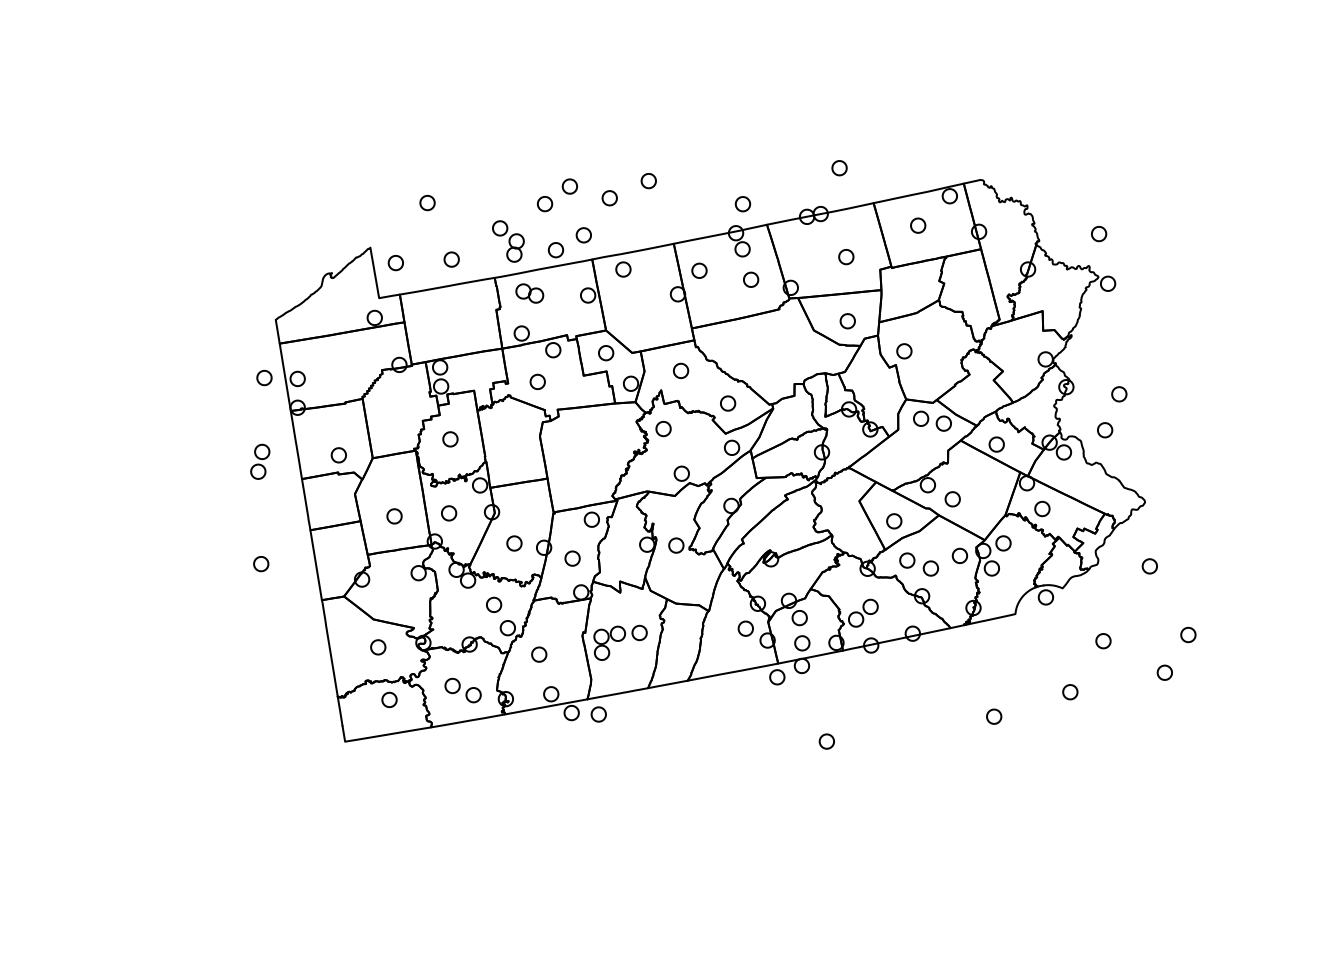
\includegraphics{Weather-Station-Code_Snowfall_files/figure-pdf/unnamed-chunk-11-1.pdf}

}

\end{figure}

\begin{Shaded}
\begin{Highlighting}[]
\CommentTok{\#Import a county layer for study site and check projections}
\CommentTok{\#counties\textless{}{-}st\_read("data/PaCounty2019\_05.shp")}
\CommentTok{\#st\_crs(counties)}
\end{Highlighting}
\end{Shaded}

\begin{Shaded}
\begin{Highlighting}[]
\CommentTok{\#Copy and Paste State Plane projection into code for StatePlane below}
\CommentTok{\#Project Weather Stations and Counties to State Plane}
\CommentTok{\#StatePlane \textless{}{-} CRS("+proj=lcc +lat\_0=39.3333333333333 +lon\_0={-}77.75 +lat\_1=40.9666666666667 \#+lat\_2=39.9333333333333 +x\_0=600000 +y\_0=0 +ellps=GRS80 +units=m +no\_defs +type=crs")}

\NormalTok{stations }\OtherTok{\textless{}{-}}\NormalTok{ merge}
\NormalTok{stations}\SpecialCharTok{$}\NormalTok{MAS }\OtherTok{\textless{}{-}}\NormalTok{ stations}\SpecialCharTok{$}\NormalTok{MeanAnnualSnowfall}
\end{Highlighting}
\end{Shaded}

\begin{Shaded}
\begin{Highlighting}[]
\NormalTok{pabox }\OtherTok{\textless{}{-}} \FunctionTok{st\_bbox}\NormalTok{(PAcounties)}
\CommentTok{\#Plot out the MAS across the study region}
\NormalTok{tmap.bubble }\OtherTok{\textless{}{-}} \FunctionTok{tm\_shape}\NormalTok{(stations, }\AttributeTok{bbox=}\NormalTok{pabox) }\SpecialCharTok{+} \FunctionTok{tm\_sf}\NormalTok{(}\AttributeTok{size =} \StringTok{"MAS"}\NormalTok{)}
\NormalTok{tmap.bubble}
\end{Highlighting}
\end{Shaded}

\begin{Shaded}
\begin{Highlighting}[]
\CommentTok{\#Create a grid onto which we will interpolate:}
\NormalTok{bb }\OtherTok{\textless{}{-}} \FunctionTok{st\_bbox}\NormalTok{(PAcounties) }\SpecialCharTok{\%\textgreater{}\%} \FunctionTok{st\_as\_sfc}\NormalTok{()}
\NormalTok{grid\_spacing }\OtherTok{\textless{}{-}} \DecValTok{5000}
\NormalTok{grid }\OtherTok{\textless{}{-}} \FunctionTok{st\_make\_grid}\NormalTok{(bb, }\AttributeTok{square =}\NormalTok{ T, }\AttributeTok{cellsize =} \FunctionTok{c}\NormalTok{(grid\_spacing, grid\_spacing)) }\SpecialCharTok{\%\textgreater{}\%} \CommentTok{\# the grid, covering bounding box}
  \FunctionTok{st\_intersection}\NormalTok{(bb) }\SpecialCharTok{\%\textgreater{}\%}
    \FunctionTok{cbind}\NormalTok{(}\FunctionTok{data.frame}\NormalTok{(}\AttributeTok{ID =} \FunctionTok{sprintf}\NormalTok{(}\FunctionTok{paste}\NormalTok{(}\StringTok{"GID\%0"}\NormalTok{,}\FunctionTok{nchar}\NormalTok{(}\FunctionTok{length}\NormalTok{(.)),}\StringTok{"d"}\NormalTok{,}\AttributeTok{sep=}\StringTok{""}\NormalTok{), }\DecValTok{1}\SpecialCharTok{:}\FunctionTok{length}\NormalTok{(.)))) }\SpecialCharTok{\%\textgreater{}\%}
    \FunctionTok{st\_sf}\NormalTok{()}
\CommentTok{\#Convert grid to a raster to use later}
\NormalTok{rgrid }\OtherTok{\textless{}{-}} \FunctionTok{rast}\NormalTok{(grid, }\AttributeTok{res=}\DecValTok{5000}\NormalTok{)}\CommentTok{\#, type="xyz",crs = albers.crs,digits=6,extent=NULL)}
\FunctionTok{plot}\NormalTok{(}\FunctionTok{st\_geometry}\NormalTok{(bb))}
\FunctionTok{plot}\NormalTok{(}\FunctionTok{st\_geometry}\NormalTok{(grid),}\AttributeTok{add=}\NormalTok{T)}
\end{Highlighting}
\end{Shaded}

\begin{figure}[H]

{\centering 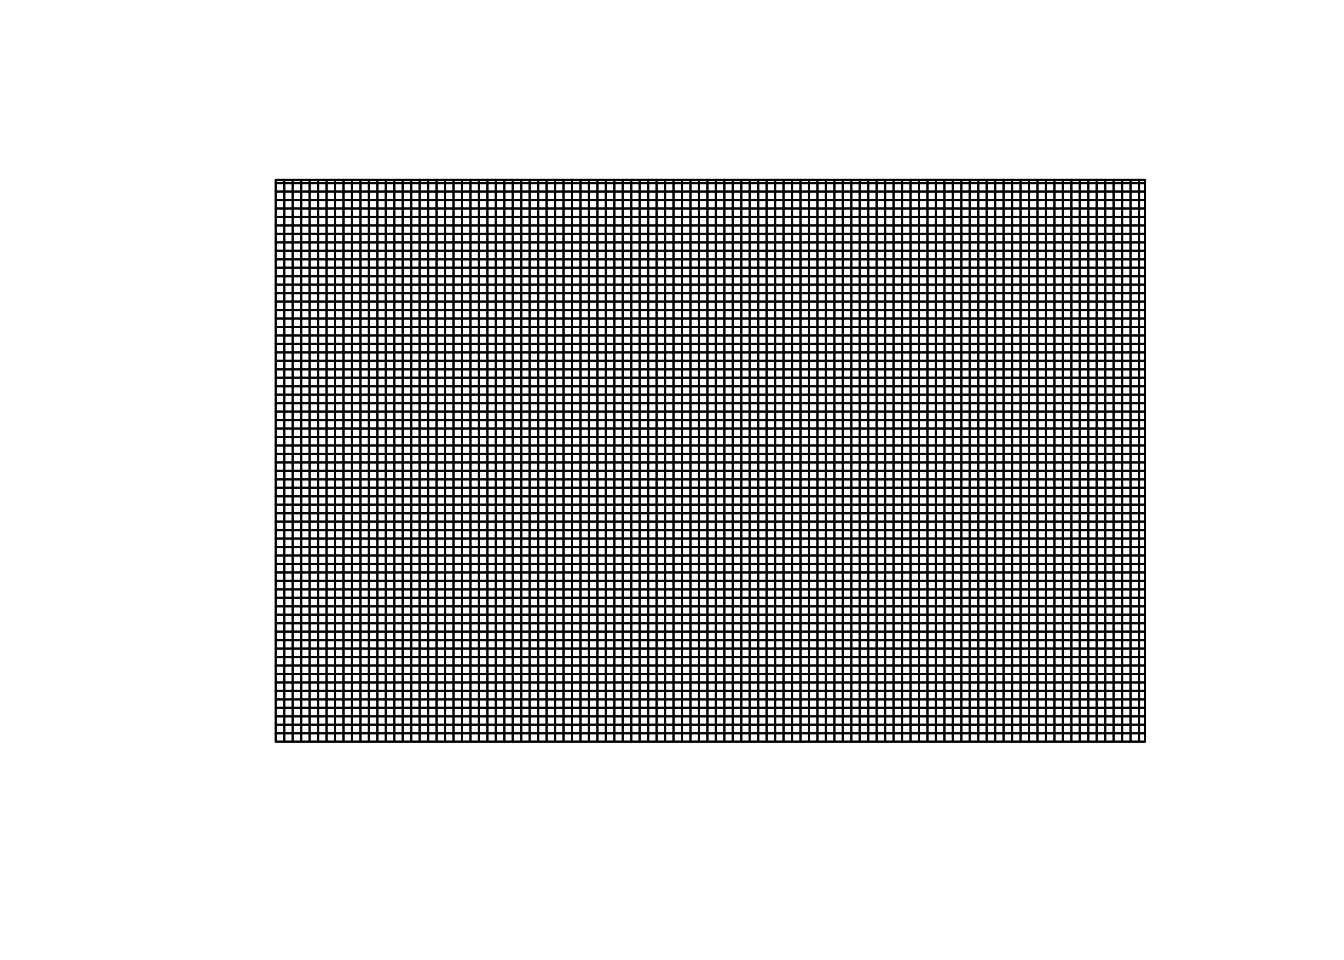
\includegraphics{Weather-Station-Code_Snowfall_files/figure-pdf/unnamed-chunk-14-1.pdf}

}

\end{figure}

\begin{Shaded}
\begin{Highlighting}[]
\CommentTok{\#Plot Weather Stations over counties}
\FunctionTok{plot}\NormalTok{(}\FunctionTok{st\_geometry}\NormalTok{(PAcounties))}
\FunctionTok{plot}\NormalTok{(}\FunctionTok{st\_geometry}\NormalTok{(stations), }\AttributeTok{add=}\NormalTok{T, }\AttributeTok{pch=}\DecValTok{16}\NormalTok{, }\AttributeTok{col=}\StringTok{"red"}\NormalTok{)}
\end{Highlighting}
\end{Shaded}

\begin{figure}[H]

{\centering 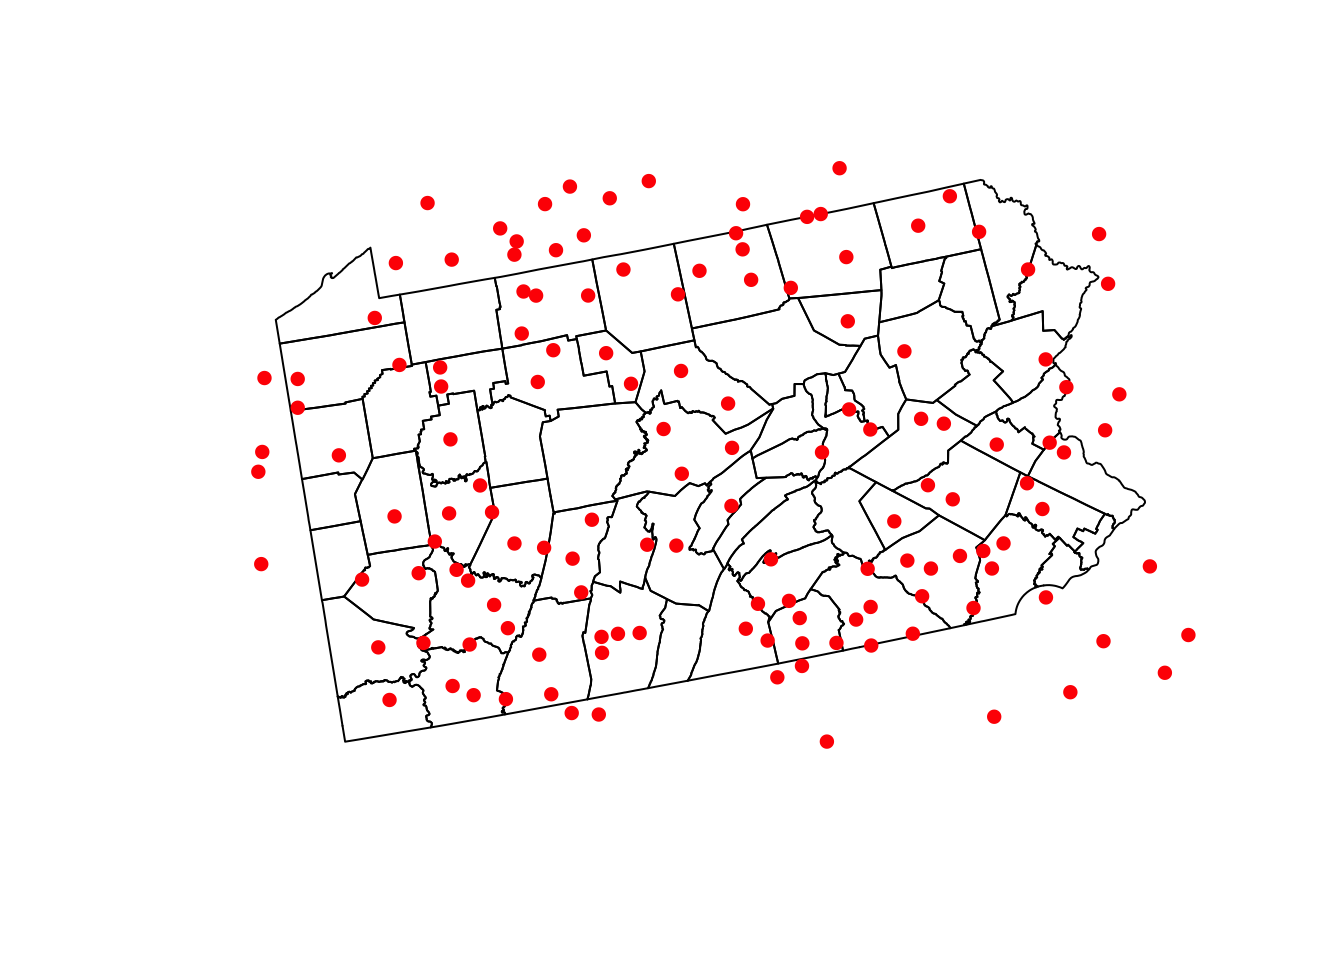
\includegraphics{Weather-Station-Code_Snowfall_files/figure-pdf/unnamed-chunk-14-2.pdf}

}

\end{figure}

nearest neighbor interpolate grid over sample points directly in R with
gstat package

\begin{Shaded}
\begin{Highlighting}[]
\NormalTok{stations2 }\OtherTok{\textless{}{-}} \FunctionTok{sf\_to\_df}\NormalTok{(stations, }\AttributeTok{fill=}\ConstantTok{TRUE}\NormalTok{)}
\NormalTok{gOK }\OtherTok{\textless{}{-}} \FunctionTok{gstat}\NormalTok{(}\AttributeTok{formula=}\NormalTok{MAS}\SpecialCharTok{\textasciitilde{}}\DecValTok{1}\NormalTok{, }\AttributeTok{data=}\NormalTok{stations2, }\AttributeTok{locations=}\SpecialCharTok{\textasciitilde{}}\NormalTok{x}\SpecialCharTok{+}\NormalTok{y, }\AttributeTok{nmax=}\DecValTok{10}\NormalTok{, }\AttributeTok{set=}\FunctionTok{list}\NormalTok{(}\AttributeTok{idp=}\DecValTok{0}\NormalTok{))}
\NormalTok{x }\OtherTok{\textless{}{-}} \FunctionTok{interpolate}\NormalTok{(rgrid, gOK,}\AttributeTok{debug.level=}\DecValTok{0}\NormalTok{)}
\FunctionTok{class}\NormalTok{(x)}
\end{Highlighting}
\end{Shaded}

\begin{verbatim}
[1] "SpatRaster"
attr(,"package")
[1] "terra"
\end{verbatim}

\begin{Shaded}
\begin{Highlighting}[]
\FunctionTok{plot}\NormalTok{(x,}\DecValTok{1}\NormalTok{)}
\FunctionTok{plot}\NormalTok{(}\FunctionTok{st\_geometry}\NormalTok{(stations), }\AttributeTok{add=}\NormalTok{T, }\AttributeTok{pch=}\DecValTok{16}\NormalTok{, }\AttributeTok{col=}\StringTok{"red"}\NormalTok{)}
\FunctionTok{plot}\NormalTok{(}\FunctionTok{st\_geometry}\NormalTok{(PAcounties), }\AttributeTok{add=}\NormalTok{T)}
\end{Highlighting}
\end{Shaded}

\begin{figure}[H]

{\centering 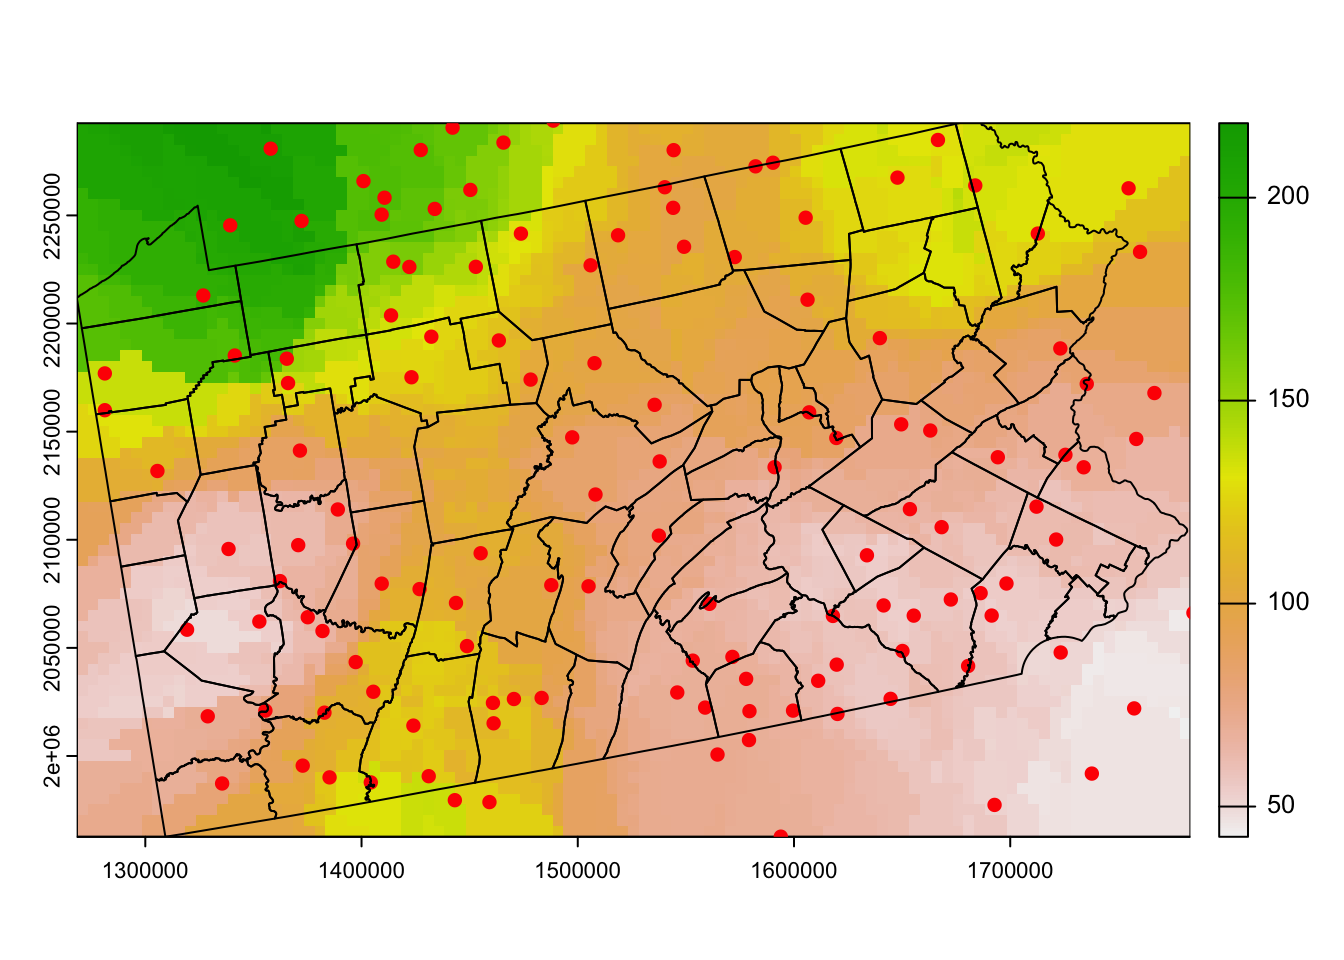
\includegraphics{Weather-Station-Code_Snowfall_files/figure-pdf/unnamed-chunk-15-1.pdf}

}

\end{figure}

nmax = maximum number of points used is 10

idp = inverse distance power is zero so that all 10 neighbors are
equally weighted

\hypertarget{importing-dynamically-downscaled-global-climate-data}{%
\chapter{Importing Dynamically Downscaled Global Climate
Data}\label{importing-dynamically-downscaled-global-climate-data}}

This exercise will provide some code for manipulating climate change
data from the Regional Climate Downscaling by copy the link into your
browser: http://regclim.coas.oregonstate.edu/data-access/index.html or
just select the link here:
\href{http://regclim.coas.oregonstate.edu/data-access/index.html}{Regional
Climate Downscaling} . IMPORTANT: For each climate projection, must
change name in first command and file name in last command.

1. Open the script ``NetCDF\_Script.Rmd'' and run code directly from the
script

2. First we need to load the packages needed for the exercise

\begin{Shaded}
\begin{Highlighting}[]
\FunctionTok{library}\NormalTok{(ncdf4)}
\end{Highlighting}
\end{Shaded}

3. Open netCDF and setting verbose=true provides details about the data
in the netcdf file including the varid. You need to know the varid to
select the variable you want to extract/summarize. Note: the dimensions
x, y, time also get a varid so you will need to subtract 3 from the
varid of interest to get the correct one.

\begin{Shaded}
\begin{Highlighting}[]
\NormalTok{dat }\OtherTok{\textless{}{-}} \FunctionTok{nc\_open}\NormalTok{(}\StringTok{"data/Monthly\_AvgMinTemp\_1995{-}99\_MPI.nc"}\NormalTok{, }\AttributeTok{write=}\ConstantTok{TRUE}\NormalTok{,  }\AttributeTok{readunlim=}\ConstantTok{TRUE}\NormalTok{, }\AttributeTok{verbose=}\ConstantTok{FALSE}\NormalTok{)  }

\CommentTok{\#Read data to load all the data from the downloaded variable into the tmin object}
\NormalTok{tmin }\OtherTok{\textless{}{-}}\NormalTok{ dat}\SpecialCharTok{$}\NormalTok{var[[}\DecValTok{1}\NormalTok{]]}

\DocumentationTok{\#\#\#\#\#\#\#\#\#\#\#\#\#\#\#\#\#\#\#\#\#\#\#\#\#\#\#\#\#\#\#\#\#\#\#\#\#}
\CommentTok{\# The following illustrates how to read the data }
\DocumentationTok{\#\#\#\#\#\#\#\#\#\#\#\#\#\#\#\#\#\#\#\#\#\#\#\#\#\#\#\#\#\#\#\#\#\#\#\#\#}
\FunctionTok{print}\NormalTok{(}\FunctionTok{paste}\NormalTok{(tmin}\SpecialCharTok{$}\NormalTok{name)) }\CommentTok{\#in this case the \textquotesingle{}field name\textquotesingle{} is TAMIN}
\end{Highlighting}
\end{Shaded}

\begin{verbatim}
[1] "TAMIN"
\end{verbatim}

\begin{Shaded}
\begin{Highlighting}[]
\CommentTok{\# Grab data for TAMIN variable and place in object df1}
\NormalTok{df1 }\OtherTok{\textless{}{-}} \FunctionTok{ncvar\_get}\NormalTok{(dat, tmin)}

\CommentTok{\#head(df1, n = 10L)\# head(x, n = 6L, ...); head returns the first data  entries, x is the object, }
\CommentTok{\#n sets the number of entries displayed. tail returns  the last of the data entries         }
\CommentTok{\# Dimensions of df1 (x, y, time)}
\FunctionTok{dim}\NormalTok{(df1)}
\end{Highlighting}
\end{Shaded}

\begin{verbatim}
[1] 37 22 49
\end{verbatim}

\begin{Shaded}
\begin{Highlighting}[]
\CommentTok{\# Dimensions can also be examined one at a time}
\FunctionTok{dim}\NormalTok{(df1)[}\DecValTok{1}\NormalTok{]     }\CommentTok{\# number of x grids (37)}
\end{Highlighting}
\end{Shaded}

\begin{verbatim}
[1] 37
\end{verbatim}

\begin{Shaded}
\begin{Highlighting}[]
\FunctionTok{dim}\NormalTok{(df1)[}\DecValTok{2}\NormalTok{]     }\CommentTok{\# number of y grids (22)}
\end{Highlighting}
\end{Shaded}

\begin{verbatim}
[1] 22
\end{verbatim}

\begin{Shaded}
\begin{Highlighting}[]
\FunctionTok{dim}\NormalTok{(df1)[}\DecValTok{3}\NormalTok{]     }\CommentTok{\# number of months in file (49)}
\end{Highlighting}
\end{Shaded}

\begin{verbatim}
[1] 49
\end{verbatim}

\begin{Shaded}
\begin{Highlighting}[]
\CommentTok{\#NOTE: FILE INCLUDES MONTHS OTHER THAN JANUARY (Jans are 1,13,25,37,49)}

\CommentTok{\# Check first element}
\NormalTok{df1[}\DecValTok{1}\NormalTok{,}\DecValTok{1}\NormalTok{,}\DecValTok{1}\NormalTok{]}
\end{Highlighting}
\end{Shaded}

\begin{verbatim}
[1] -2.499621
\end{verbatim}

\begin{Shaded}
\begin{Highlighting}[]
\CommentTok{\# Check first January for all x,y}
\NormalTok{df1[,,}\DecValTok{1}\NormalTok{]}
\end{Highlighting}
\end{Shaded}

\begin{Shaded}
\begin{Highlighting}[]
\CommentTok{\#Create a new matrix which is monthly averages for each grid cell. Make the new  matrix the }
\CommentTok{\#same size (i.e. same number of rows and columns as there are in the dataframe df1}
\NormalTok{sum1 }\OtherTok{\textless{}{-}} \FunctionTok{array}\NormalTok{(}\AttributeTok{data=}\ConstantTok{NA}\NormalTok{, }\FunctionTok{c}\NormalTok{(}\FunctionTok{dim}\NormalTok{(df1)[}\DecValTok{1}\NormalTok{],}\FunctionTok{dim}\NormalTok{(df1)[}\DecValTok{2}\NormalTok{] ))}
\FunctionTok{dim}\NormalTok{(sum1)}
\end{Highlighting}
\end{Shaded}

\begin{verbatim}
[1] 37 22
\end{verbatim}

\begin{Shaded}
\begin{Highlighting}[]
\CommentTok{\# Create January mean TAMIN for each x{-}y coordinate}
\ControlFlowTok{for}\NormalTok{(i }\ControlFlowTok{in} \DecValTok{1}\SpecialCharTok{:}\FunctionTok{dim}\NormalTok{(df1)[}\DecValTok{1}\NormalTok{])\{ }\CommentTok{\# loop over x{-}coords}
    \ControlFlowTok{for}\NormalTok{(j }\ControlFlowTok{in} \DecValTok{1}\SpecialCharTok{:}\FunctionTok{dim}\NormalTok{(df1)[}\DecValTok{2}\NormalTok{])\{ }\CommentTok{\# loop over y{-}coords}
\NormalTok{        sum1[i, j] }\OtherTok{\textless{}{-}}\NormalTok{ (df1[i,j,}\DecValTok{1}\NormalTok{]}\SpecialCharTok{+}\NormalTok{df1[i,j,}\DecValTok{13}\NormalTok{]}\SpecialCharTok{+}\NormalTok{df1[i,j,}\DecValTok{25}\NormalTok{]}\SpecialCharTok{+}\NormalTok{df1[i,j,}\DecValTok{37}\NormalTok{]}\SpecialCharTok{+}\NormalTok{df1[i,j,}\DecValTok{49}\NormalTok{])}\SpecialCharTok{/}\DecValTok{5}
\NormalTok{    \}}
\NormalTok{\}}

\DocumentationTok{\#\#\#\#\#\#\#\#\#\#\#\#\#\#\#\#\#\#\#\#\#\#\#\#\#\#\#\#\#\#\#\#\#\#\#\#\#\#\#\#\#\#\#\#\#\#\#\#\#\#\#\#\#\#\#\#\#\#\#}
\DocumentationTok{\#\#\#\#\#\#\#\#\#\#\#\#\#\#\#\#\#\#\#\#\#\#\#\#\#\#\#\#\#\#\#\#\#\#\#\#\#\#\#\#\#\#\#\#\#\#\#\#\#\#\#\#\#\#\#\#\#\#\#}
\CommentTok{\# Create netcdf file from sum1 (contains matrix of new data)}
\DocumentationTok{\#\#\#\#\#\#\#\#\#\#\#\#\#\#\#\#\#\#\#\#\#\#\#\#\#\#\#\#\#\#\#\#\#\#\#\#\#\#\#\#\#\#\#\#\#\#\#\#\#\#\#\#\#\#\#\#\#\#\#}
\CommentTok{\# Get x and y coordinates from original "dat" ncdf file}
\NormalTok{x  }\OtherTok{=} \FunctionTok{ncvar\_get}\NormalTok{(}\AttributeTok{nc=}\NormalTok{dat,}\AttributeTok{varid=}\StringTok{"x"}\NormalTok{)   }
\NormalTok{y  }\OtherTok{=} \FunctionTok{ncvar\_get}\NormalTok{(}\AttributeTok{nc=}\NormalTok{dat,}\AttributeTok{varid=}\StringTok{"y"}\NormalTok{)  }

\CommentTok{\# Check dimensions}
\FunctionTok{length}\NormalTok{(x)}
\end{Highlighting}
\end{Shaded}

\begin{verbatim}
[1] 37
\end{verbatim}

\begin{Shaded}
\begin{Highlighting}[]
\FunctionTok{length}\NormalTok{(y)}
\end{Highlighting}
\end{Shaded}

\begin{verbatim}
[1] 22
\end{verbatim}

\begin{Shaded}
\begin{Highlighting}[]
\FunctionTok{dim}\NormalTok{(sum1)}
\end{Highlighting}
\end{Shaded}

\begin{verbatim}
[1] 37 22
\end{verbatim}

\begin{Shaded}
\begin{Highlighting}[]
\DocumentationTok{\#\# define the netcdf coordinate variables {-} note that these are coming from the dat}
\CommentTok{\#file with actual values}
\NormalTok{dim1 }\OtherTok{=} \FunctionTok{ncdim\_def}\NormalTok{( }\StringTok{"X"}\NormalTok{,}\StringTok{"meters"}\NormalTok{, }\FunctionTok{as.double}\NormalTok{(x))}
\NormalTok{dim2 }\OtherTok{=} \FunctionTok{ncdim\_def}\NormalTok{( }\StringTok{"Y"}\NormalTok{,}\StringTok{"meters"}\NormalTok{, }\FunctionTok{as.double}\NormalTok{(y))}

\DocumentationTok{\#\# define the EMPTY (climate) netcdf variable and define names that will be used in the }
\CommentTok{\#var.def.ncdf function}
\CommentTok{\# Define climate variable names}
\NormalTok{    new.name }\OtherTok{\textless{}{-}} \StringTok{\textquotesingle{}mintemp\textquotesingle{}}
\CommentTok{\# Define units of measurement for variable}
\NormalTok{    units }\OtherTok{\textless{}{-}} \StringTok{\textquotesingle{}degreesC\textquotesingle{}}
\CommentTok{\# Define long name for variable}
\NormalTok{    long.name }\OtherTok{\textless{}{-}} \StringTok{\textquotesingle{}Jan average min temperature\textquotesingle{}}

\NormalTok{varz }\OtherTok{=} \FunctionTok{ncvar\_def}\NormalTok{(new.name,units, }\FunctionTok{list}\NormalTok{(dim1,dim2), }\SpecialCharTok{{-}}\DecValTok{1}\NormalTok{, }
          \AttributeTok{longname=}\NormalTok{long.name)}

\CommentTok{\# associate the netcdf variable with a netcdf file   }
\CommentTok{\# put the variable into the file, and close}

\NormalTok{nc.ex }\OtherTok{=} \FunctionTok{nc\_create}\NormalTok{( }\StringTok{"MPI1999{-}95.nc"}\NormalTok{, varz )}
\FunctionTok{ncvar\_put}\NormalTok{(nc.ex, varz, sum1)}
\FunctionTok{nc\_close}\NormalTok{(nc.ex)}
\end{Highlighting}
\end{Shaded}

\part{Movement Methods}

\hypertarget{movement-methods}{%
\chapter{Movement Methods}\label{movement-methods}}

\hypertarget{importing-datasets-from-a-web-source}{%
\section{Importing datasets from a web
source}\label{importing-datasets-from-a-web-source}}

Movebank.org is a cloud-based repository for relocation data from
GPS-collared or VHF-collared animals. It provides a storage facility in
the cloud that can serve as a backup for your data or a transfer portal
to share data among colleagues or interested researchers. Similar to any
email account, each user has a Movebank account that has a login and
password to gain access to your data. Administration privileges can be
given to anyone with an account for viewing and downloading data.

1. Open the script ``DMAdeerMovebank.Rmd'' and run code directly from
the script

2. First we need to load the packages needed for the exercise

\begin{Shaded}
\begin{Highlighting}[]
\FunctionTok{library}\NormalTok{(move)}
\FunctionTok{library}\NormalTok{(RCurl)}
\FunctionTok{library}\NormalTok{(circular)}
\end{Highlighting}
\end{Shaded}

3. Next we are going to the \href{https://www.movebank.org/}{Movebank}
home page and explore what it has to offer. Need to create an account or
select a dataset that does not require permission to use.

\begin{Shaded}
\begin{Highlighting}[]
\NormalTok{login }\OtherTok{\textless{}{-}} \FunctionTok{movebankLogin}\NormalTok{(}\AttributeTok{username=}\StringTok{"wdwalter"}\NormalTok{, }\AttributeTok{password=}\StringTok{"XXXXX"}\NormalTok{)}
\end{Highlighting}
\end{Shaded}

\begin{Shaded}
\begin{Highlighting}[]
\NormalTok{deer }\OtherTok{\textless{}{-}} \FunctionTok{getMovebankData}\NormalTok{(}\AttributeTok{study=}\StringTok{"DMA White{-}tailed Deer 2018 Pennsylvania USA"}\NormalTok{,}
                        \AttributeTok{login=}\NormalTok{login, }\AttributeTok{moveObject=}\ConstantTok{TRUE}\NormalTok{)}
\FunctionTok{n.indiv}\NormalTok{(deer)}
\FunctionTok{n.locs}\NormalTok{(deer)}
\CommentTok{\#Plot the first deer in the stack}
\FunctionTok{plot}\NormalTok{(deer[[}\DecValTok{1}\NormalTok{]])}

\CommentTok{\#Now we will select a single deer to explore more}
\NormalTok{deer1 }\OtherTok{\textless{}{-}}\NormalTok{ deer[[}\StringTok{\textquotesingle{}X20212\_20242F\textquotesingle{}}\NormalTok{]]}
\FunctionTok{plot}\NormalTok{(deer1)}

\CommentTok{\#Select and plot locations of the initial 2 deer in your list}
\NormalTok{deer2 }\OtherTok{\textless{}{-}}\NormalTok{ deer[[}\FunctionTok{c}\NormalTok{(}\DecValTok{1}\NormalTok{,}\DecValTok{2}\NormalTok{)]]}
\FunctionTok{plot}\NormalTok{(deer2)}
\CommentTok{\#Determine names of initial 2 deer selected above}
\FunctionTok{namesIndiv}\NormalTok{(deer2)}
\end{Highlighting}
\end{Shaded}

\hypertarget{movement-trajectories}{%
\chapter{Movement Trajectories}\label{movement-trajectories}}

We will start with simply creating trajectories between successive
locations. As stated previously, there are 2 types of trajectories but
their are also 2 forms of Type II trajectories if we have time recorded.
Depending on the duration between locations we can have uniform time lag
between successive relocations termed regular trajectories and
non-uniform time lag that results in irregular trajectories. We will
begin this section with simply creating irregular trajectories from
relocation data because, even though we set up a time schedule to
collection locations at uniform times, climate, habitat, and satellites
do not always permit such schedules of data collection.

1. Open the script ``MovementScript.Rmd'' and run code directly from the
script

2. First we need to load the packages needed for the exercise

\begin{Shaded}
\begin{Highlighting}[]
\FunctionTok{library}\NormalTok{(adehabitatLT)}
\FunctionTok{library}\NormalTok{(chron)}
\FunctionTok{library}\NormalTok{(sf)}
\end{Highlighting}
\end{Shaded}

3. Now let's have a separate section of code to include projection
information we will use throughout the exercise. In previous versions,
these lines of code were within each block of code

\begin{Shaded}
\begin{Highlighting}[]
\NormalTok{ll.crs }\OtherTok{\textless{}{-}} \FunctionTok{st\_crs}\NormalTok{(}\DecValTok{4269}\NormalTok{)}
\NormalTok{utm.crs }\OtherTok{\textless{}{-}} \FunctionTok{st\_crs}\NormalTok{(}\DecValTok{9001}\NormalTok{)}
\NormalTok{albers.crs }\OtherTok{\textless{}{-}} \FunctionTok{st\_crs}\NormalTok{(}\DecValTok{5070}\NormalTok{)}
\end{Highlighting}
\end{Shaded}

4. We are again going to be using more of the mule deer dataset than
from the earlier exercises

\begin{Shaded}
\begin{Highlighting}[]
\NormalTok{muleys }\OtherTok{\textless{}{-}}\FunctionTok{read.csv}\NormalTok{(}\StringTok{"data/DCmuleysedited.csv"}\NormalTok{, }\AttributeTok{header=}\NormalTok{T)}
\end{Highlighting}
\end{Shaded}

5. Check for duplicate locations in dataset. The reason for this is very
important and will be apparent shortly.

\begin{Shaded}
\begin{Highlighting}[]
\CommentTok{\#Check for duplicate locations in dataset}
\FunctionTok{summary}\NormalTok{(}\FunctionTok{duplicated}\NormalTok{(muleys))}
\end{Highlighting}
\end{Shaded}

\begin{verbatim}
   Mode   FALSE 
logical    9752 
\end{verbatim}

6. For trajectories of type II (time recorded), the conversion of the
date to the format POSIX needs to be done to get proper digits of date
into R.

\begin{Shaded}
\begin{Highlighting}[]
\NormalTok{da }\OtherTok{\textless{}{-}} \FunctionTok{as.POSIXct}\NormalTok{(}\FunctionTok{strptime}\NormalTok{(muleys}\SpecialCharTok{$}\NormalTok{GPSFixTime,}\AttributeTok{format=}\StringTok{"\%Y.\%m.\%d \%H:\%M:\%S"}\NormalTok{))}
\NormalTok{muleys}\SpecialCharTok{$}\NormalTok{da }\OtherTok{\textless{}{-}}\NormalTok{ da}

\NormalTok{timediff }\OtherTok{\textless{}{-}} \FunctionTok{diff}\NormalTok{(muleys}\SpecialCharTok{$}\NormalTok{da)}\SpecialCharTok{*}\DecValTok{60}
\NormalTok{muleys }\OtherTok{\textless{}{-}}\NormalTok{muleys[}\SpecialCharTok{{-}}\DecValTok{1}\NormalTok{,]}
\NormalTok{muleys}\SpecialCharTok{$}\NormalTok{timediff }\OtherTok{\textless{}{-}}\FunctionTok{as.numeric}\NormalTok{(}\FunctionTok{abs}\NormalTok{(timediff)) }

\CommentTok{\#Remove outlier locations}
\NormalTok{coords }\OtherTok{\textless{}{-}} \FunctionTok{st\_as\_sf}\NormalTok{(muleys, }\AttributeTok{coords =} \FunctionTok{c}\NormalTok{(}\StringTok{"Long"}\NormalTok{, }\StringTok{"Lat"}\NormalTok{), }\AttributeTok{crs =}\NormalTok{ ll.crs)}
\FunctionTok{plot}\NormalTok{(}\FunctionTok{st\_geometry}\NormalTok{(coords),}\AttributeTok{axes=}\NormalTok{T)}
\end{Highlighting}
\end{Shaded}

\begin{figure}[H]

{\centering \includegraphics{MovementScript_files/figure-pdf/unnamed-chunk-5-1.pdf}

}

\end{figure}

\begin{Shaded}
\begin{Highlighting}[]
\NormalTok{deer.spdf }\OtherTok{\textless{}{-}} \FunctionTok{st\_crop}\NormalTok{(coords, }\AttributeTok{xmin=}\SpecialCharTok{{-}}\FloatTok{107.0}\NormalTok{,}\AttributeTok{xmax=}\SpecialCharTok{{-}}\FloatTok{110.5}\NormalTok{,}\AttributeTok{ymin=}\FloatTok{37.8}\NormalTok{,}\AttributeTok{ymax=}\FloatTok{39.0}\NormalTok{)}\CommentTok{\#Visually identified based on previous plot}
\end{Highlighting}
\end{Shaded}

\begin{verbatim}
Warning: attribute variables are assumed to be spatially constant throughout
all geometries
\end{verbatim}

\begin{Shaded}
\begin{Highlighting}[]
\FunctionTok{plot}\NormalTok{(}\FunctionTok{st\_geometry}\NormalTok{(deer.spdf),}\AttributeTok{axes=}\NormalTok{T)}
\end{Highlighting}
\end{Shaded}

\begin{figure}[H]

{\centering \includegraphics{MovementScript_files/figure-pdf/unnamed-chunk-5-2.pdf}

}

\end{figure}

\begin{Shaded}
\begin{Highlighting}[]
\CommentTok{\#Project deer.spdf to Albers as in previous exercise}
\NormalTok{deer.albers }\OtherTok{\textless{}{-}}\FunctionTok{st\_transform}\NormalTok{(deer.spdf, }\AttributeTok{crs=}\NormalTok{albers.crs)}
\FunctionTok{plot}\NormalTok{(}\FunctionTok{st\_geometry}\NormalTok{(deer.albers),}\AttributeTok{axes=}\NormalTok{T)}
\end{Highlighting}
\end{Shaded}

\begin{figure}[H]

{\centering 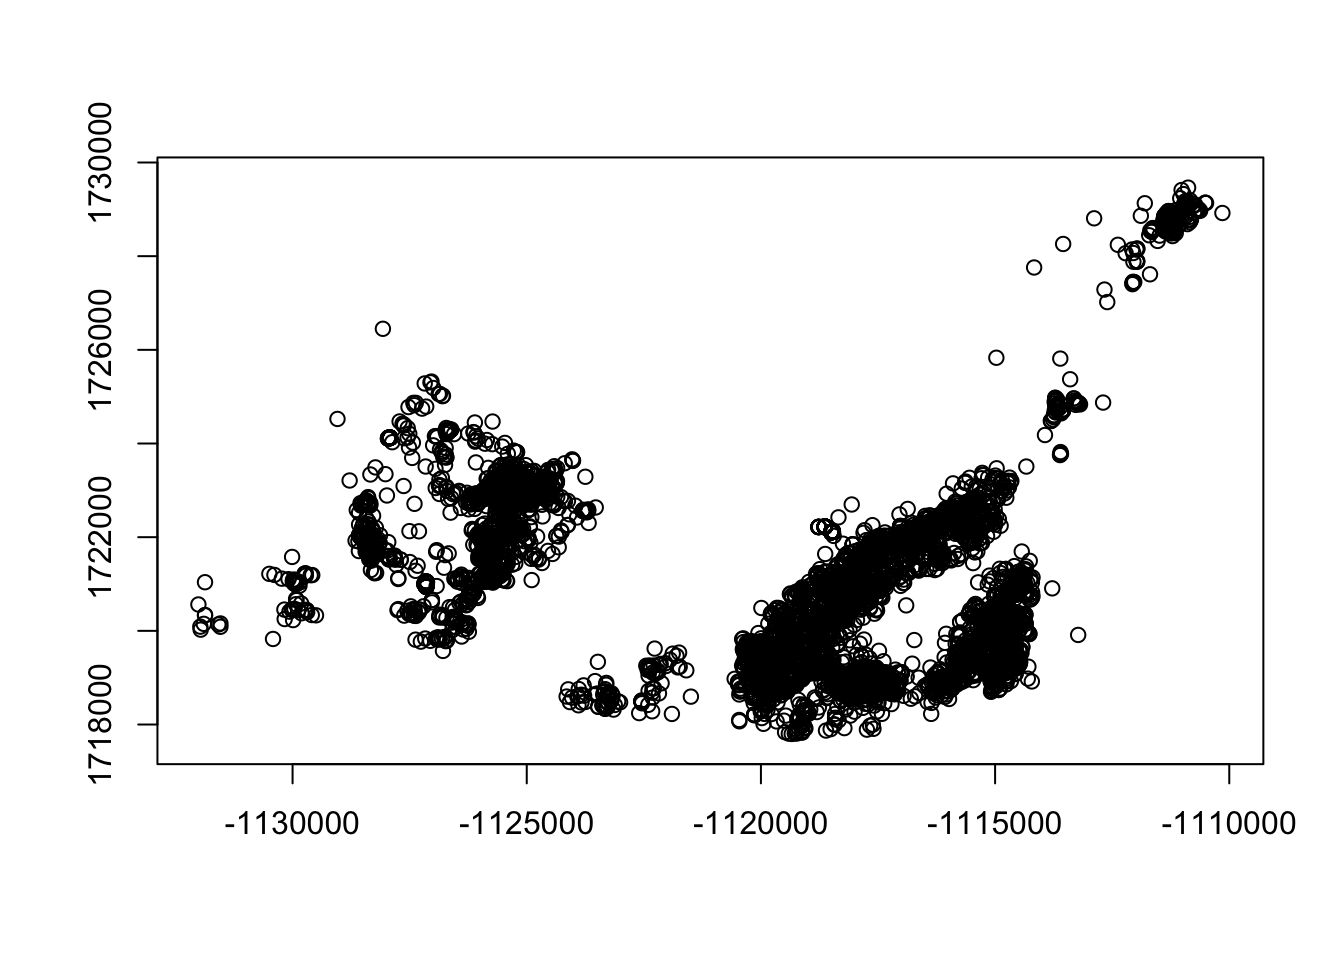
\includegraphics{MovementScript_files/figure-pdf/unnamed-chunk-5-3.pdf}

}

\end{figure}

6. Now create an object of class ``ltraj'' by animal using the ID field
and display by each individual (i.e., ltraj{[}1{]})

\begin{Shaded}
\begin{Highlighting}[]
\NormalTok{ltraj }\OtherTok{\textless{}{-}} \FunctionTok{as.ltraj}\NormalTok{(}\FunctionTok{st\_coordinates}\NormalTok{(deer.albers),deer.albers}\SpecialCharTok{$}\NormalTok{da,}\AttributeTok{id=}\NormalTok{deer.albers}\SpecialCharTok{$}\NormalTok{id)}
\FunctionTok{head}\NormalTok{(ltraj[}\DecValTok{1}\NormalTok{])}\CommentTok{\#Describes the trajectory}
\end{Highlighting}
\end{Shaded}

\begin{verbatim}

*********** List of class ltraj ***********

Type of the traject: Type II (time recorded)
* Time zone unspecified: dates printed in user time zone *
Irregular traject. Variable time lag between two locs

Characteristics of the bursts:
   id burst nb.reloc NAs          date.begin            date.end
1 D12   D12      101   0 2011-10-12 03:00:48 2011-10-24 21:00:48


 infolocs provided. The following variables are available:
[1] "pkey"
\end{verbatim}

\begin{Shaded}
\begin{Highlighting}[]
\FunctionTok{plot}\NormalTok{(ltraj)}\CommentTok{\#plot all trajectories created}
\end{Highlighting}
\end{Shaded}

\begin{figure}[H]

{\centering \includegraphics{MovementScript_files/figure-pdf/unnamed-chunk-6-1.pdf}

}

\end{figure}

\begin{Shaded}
\begin{Highlighting}[]
\CommentTok{\#Plot each trajectory separately}
\FunctionTok{plot}\NormalTok{(ltraj[}\DecValTok{1}\NormalTok{])}
\end{Highlighting}
\end{Shaded}

\begin{figure}[H]

{\centering \includegraphics{MovementScript_files/figure-pdf/unnamed-chunk-6-2.pdf}

}

\end{figure}

\begin{Shaded}
\begin{Highlighting}[]
\FunctionTok{plot}\NormalTok{(ltraj[}\DecValTok{2}\NormalTok{])}
\end{Highlighting}
\end{Shaded}

\begin{figure}[H]

{\centering 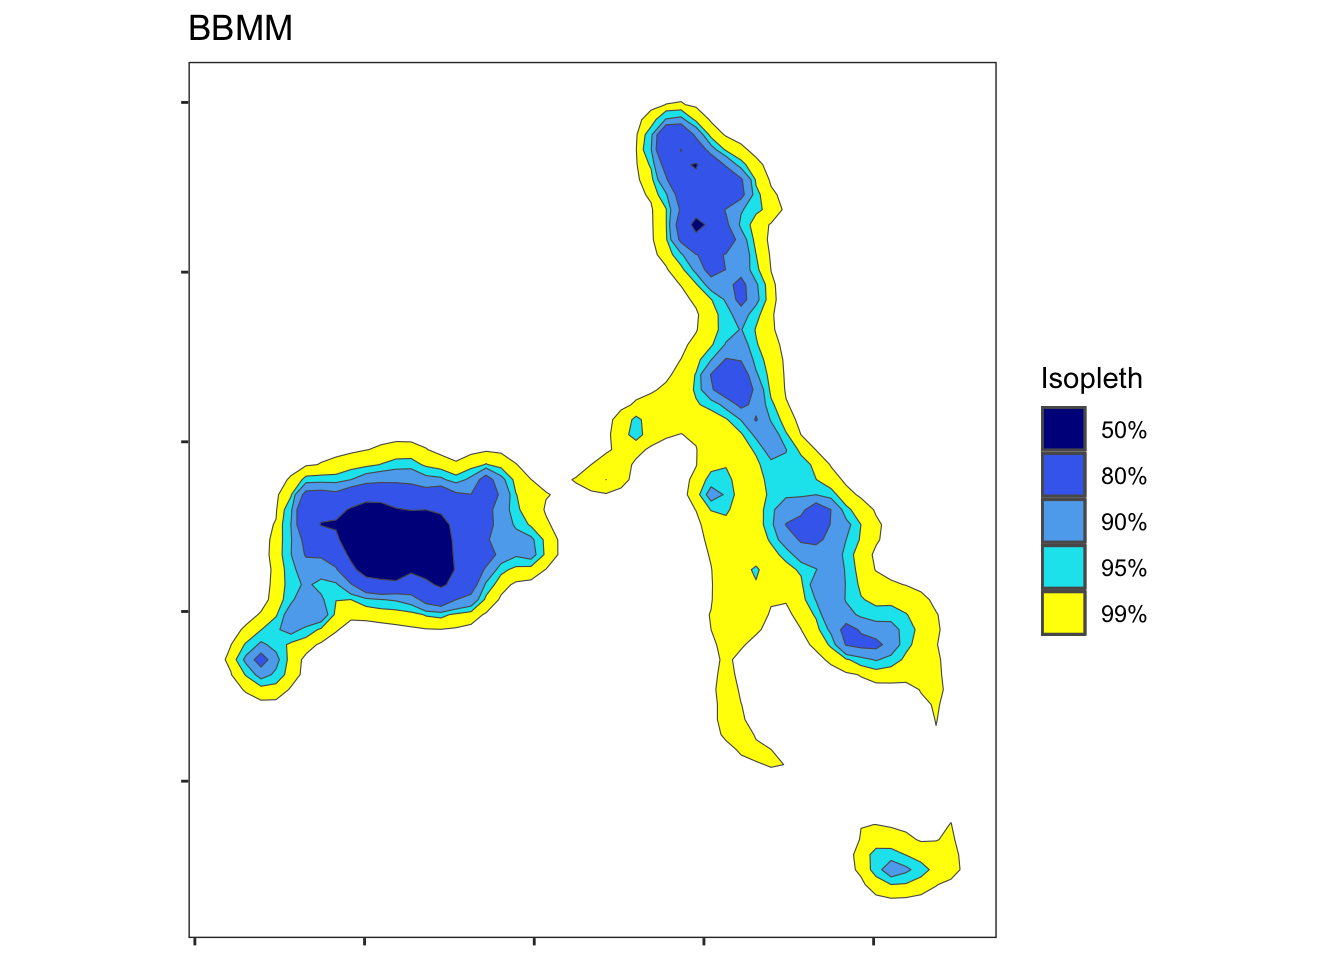
\includegraphics{MovementScript_files/figure-pdf/unnamed-chunk-6-3.pdf}

}

\end{figure}

\begin{Shaded}
\begin{Highlighting}[]
\FunctionTok{plot}\NormalTok{(ltraj[}\DecValTok{3}\NormalTok{])}
\end{Highlighting}
\end{Shaded}

\begin{figure}[H]

{\centering 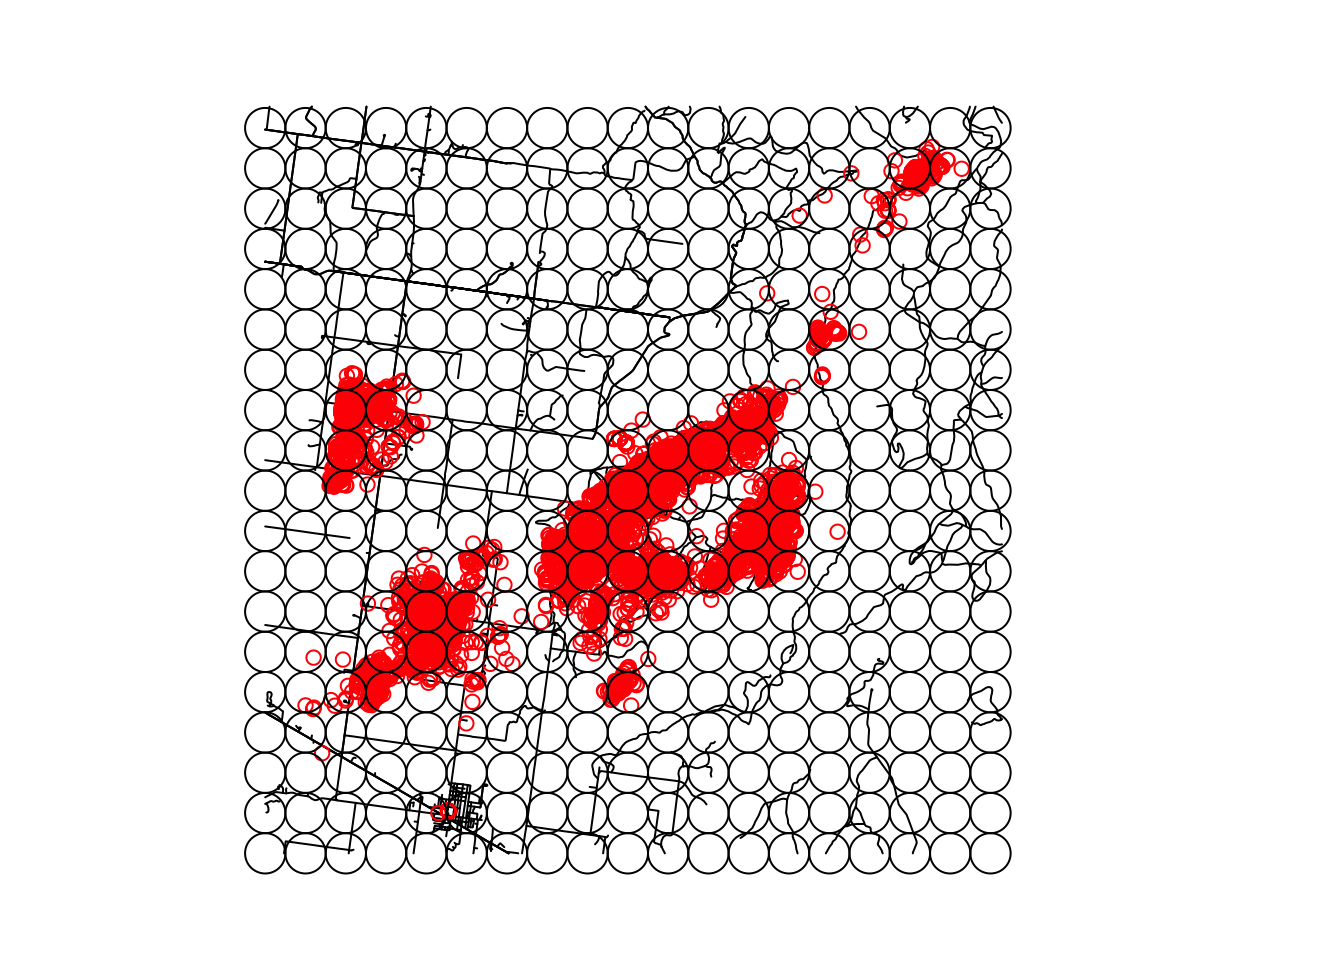
\includegraphics{MovementScript_files/figure-pdf/unnamed-chunk-6-4.pdf}

}

\end{figure}

\begin{Shaded}
\begin{Highlighting}[]
\FunctionTok{plot}\NormalTok{(ltraj[}\DecValTok{4}\NormalTok{])}
\end{Highlighting}
\end{Shaded}

\begin{figure}[H]

{\centering 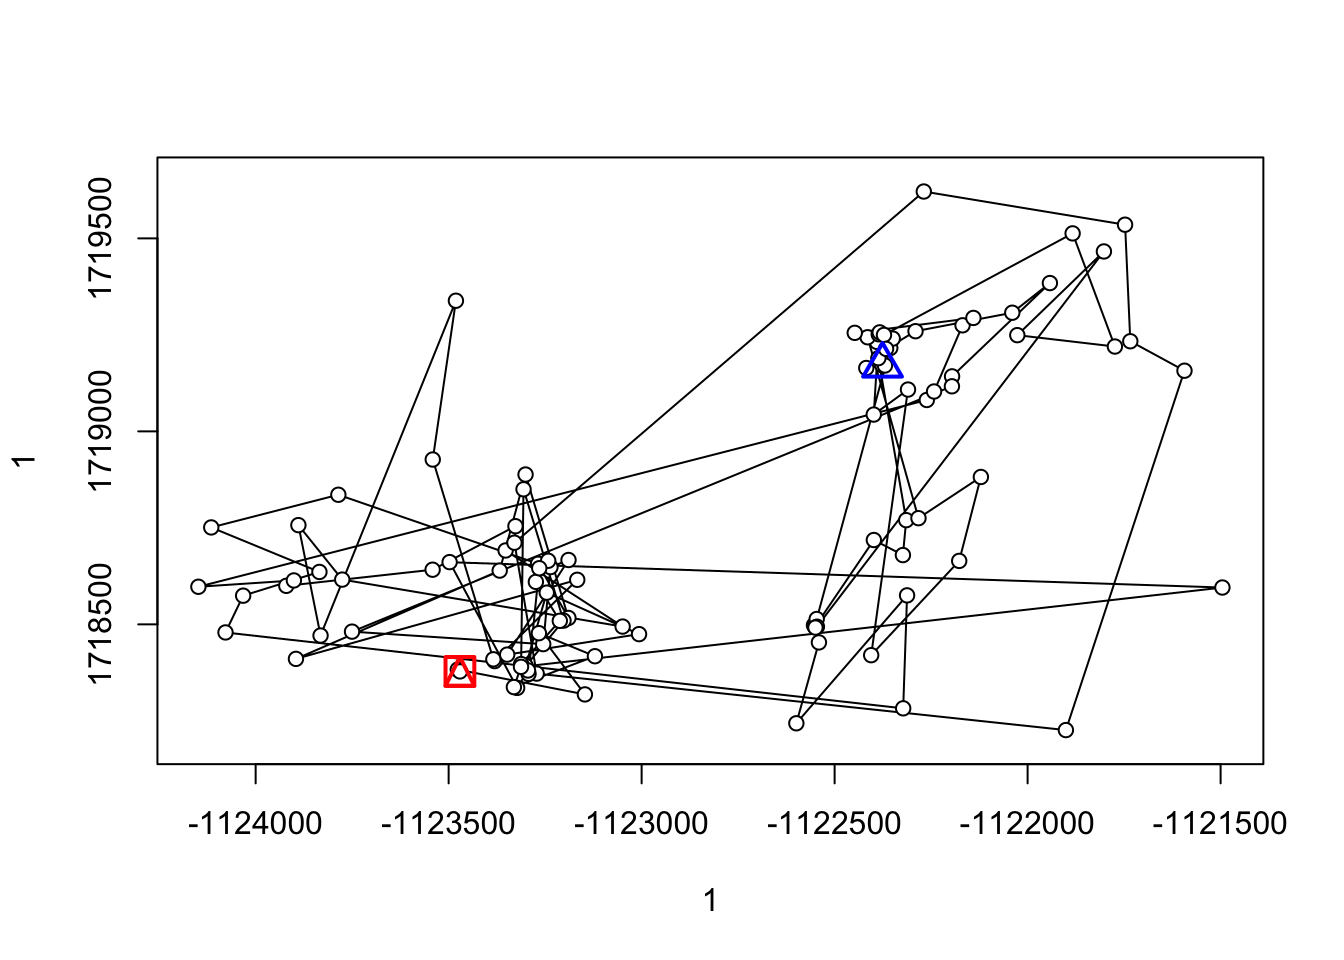
\includegraphics{MovementScript_files/figure-pdf/unnamed-chunk-6-5.pdf}

}

\end{figure}

\begin{Shaded}
\begin{Highlighting}[]
\FunctionTok{plot}\NormalTok{(ltraj[}\DecValTok{5}\NormalTok{])}
\end{Highlighting}
\end{Shaded}

\begin{figure}[H]

{\centering 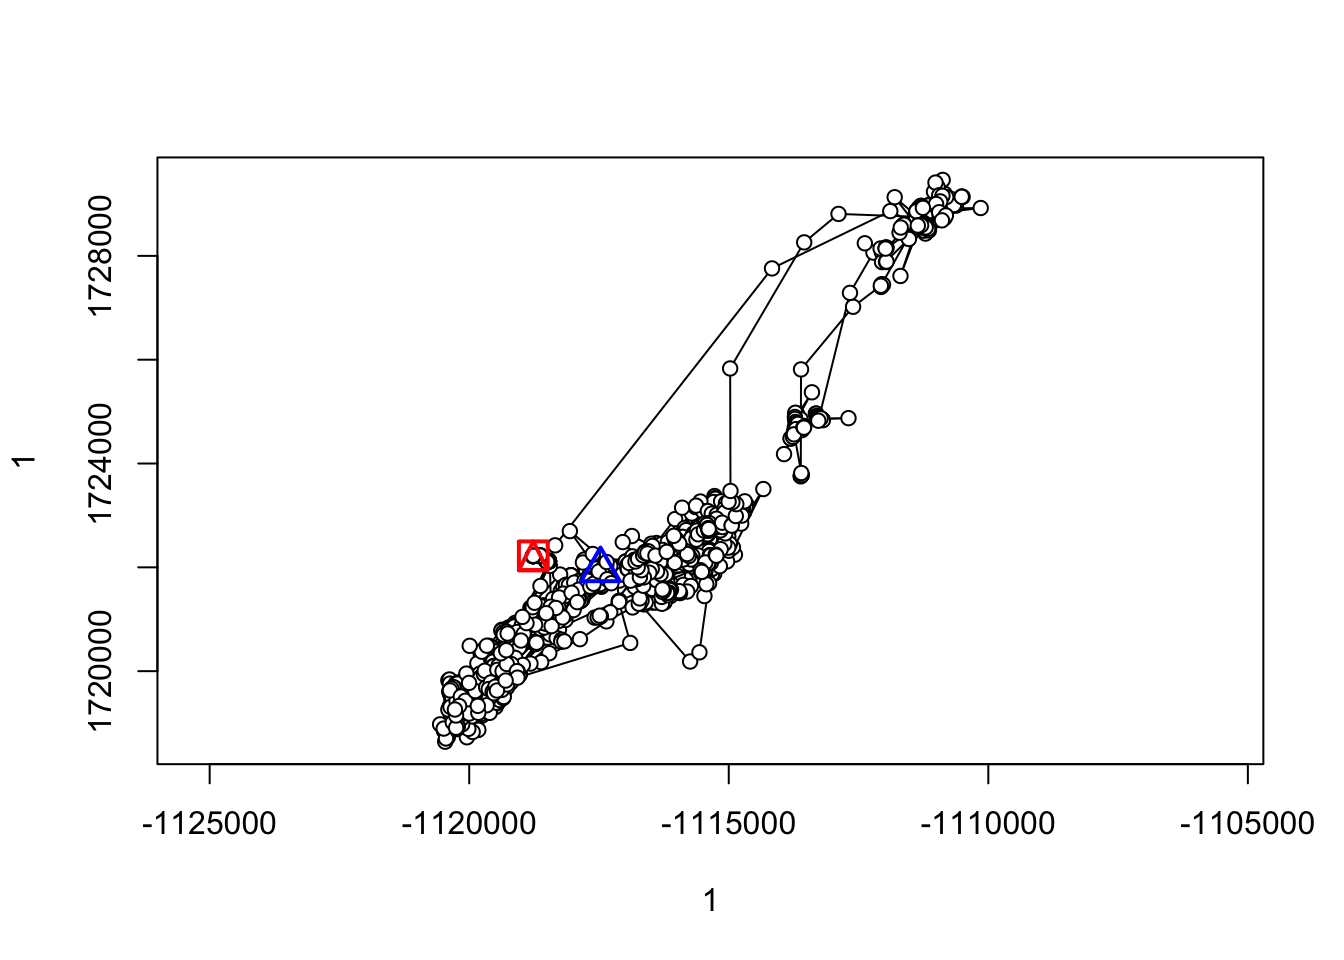
\includegraphics{MovementScript_files/figure-pdf/unnamed-chunk-6-6.pdf}

}

\end{figure}

\begin{Shaded}
\begin{Highlighting}[]
\FunctionTok{plot}\NormalTok{(ltraj[}\DecValTok{6}\NormalTok{])}
\end{Highlighting}
\end{Shaded}

\begin{figure}[H]

{\centering 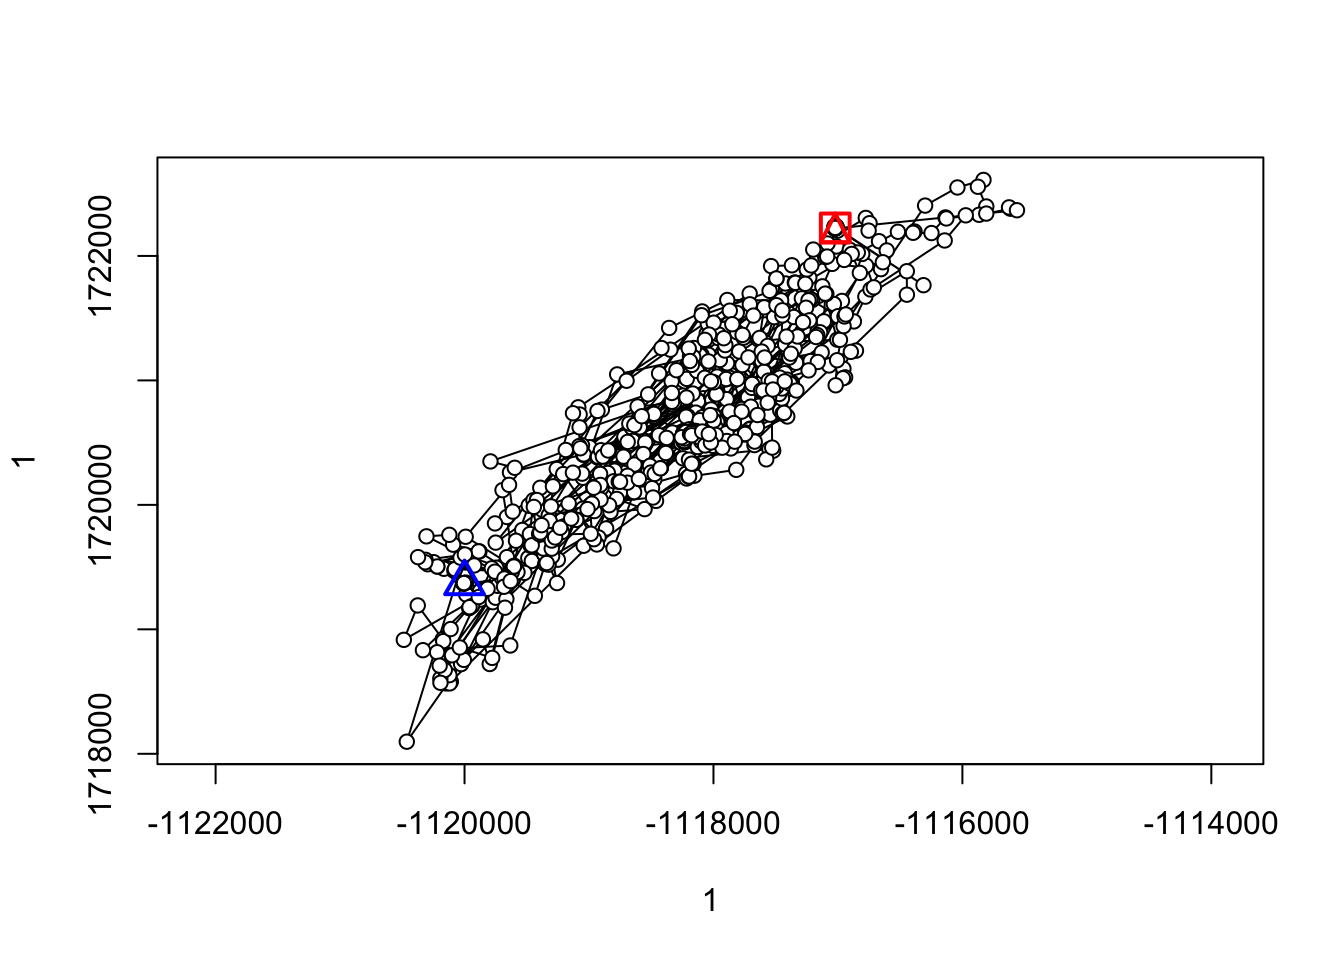
\includegraphics{MovementScript_files/figure-pdf/unnamed-chunk-6-7.pdf}

}

\end{figure}

7. Create a histogram of time lag (i.e., interval) and distance between
successive locations for each deer. This is a nice way to inspect the
time lag between locations as you don't want to include a location if
too much time has passed since the previous and it also shows why a
trajectory is irregular.

\begin{Shaded}
\begin{Highlighting}[]
\FunctionTok{hist}\NormalTok{(ltraj[}\DecValTok{1}\NormalTok{], }\StringTok{"dt"}\NormalTok{, }\AttributeTok{freq =} \ConstantTok{TRUE}\NormalTok{)}
\FunctionTok{hist}\NormalTok{(ltraj[}\DecValTok{1}\NormalTok{], }\StringTok{"dist"}\NormalTok{, }\AttributeTok{freq =} \ConstantTok{TRUE}\NormalTok{)}
\FunctionTok{hist}\NormalTok{(ltraj[}\DecValTok{2}\NormalTok{], }\StringTok{"dt"}\NormalTok{, }\AttributeTok{freq =} \ConstantTok{TRUE}\NormalTok{)}
\FunctionTok{hist}\NormalTok{(ltraj[}\DecValTok{2}\NormalTok{], }\StringTok{"dist"}\NormalTok{, }\AttributeTok{freq =} \ConstantTok{TRUE}\NormalTok{)}
\FunctionTok{hist}\NormalTok{(ltraj[}\DecValTok{3}\NormalTok{], }\StringTok{"dt"}\NormalTok{, }\AttributeTok{freq =} \ConstantTok{TRUE}\NormalTok{)}
\FunctionTok{hist}\NormalTok{(ltraj[}\DecValTok{3}\NormalTok{], }\StringTok{"dist"}\NormalTok{, }\AttributeTok{freq =} \ConstantTok{TRUE}\NormalTok{)}
\FunctionTok{hist}\NormalTok{(ltraj[}\DecValTok{4}\NormalTok{], }\StringTok{"dt"}\NormalTok{, }\AttributeTok{freq =} \ConstantTok{TRUE}\NormalTok{)}
\FunctionTok{hist}\NormalTok{(ltraj[}\DecValTok{4}\NormalTok{], }\StringTok{"dist"}\NormalTok{, }\AttributeTok{freq =} \ConstantTok{TRUE}\NormalTok{)}
\FunctionTok{hist}\NormalTok{(ltraj[}\DecValTok{5}\NormalTok{], }\StringTok{"dt"}\NormalTok{, }\AttributeTok{freq =} \ConstantTok{TRUE}\NormalTok{)}
\FunctionTok{hist}\NormalTok{(ltraj[}\DecValTok{5}\NormalTok{], }\StringTok{"dist"}\NormalTok{, }\AttributeTok{freq =} \ConstantTok{TRUE}\NormalTok{)}
\FunctionTok{hist}\NormalTok{(ltraj[}\DecValTok{6}\NormalTok{], }\StringTok{"dt"}\NormalTok{, }\AttributeTok{freq =} \ConstantTok{TRUE}\NormalTok{)}
\FunctionTok{hist}\NormalTok{(ltraj[}\DecValTok{6}\NormalTok{], }\StringTok{"dist"}\NormalTok{, }\AttributeTok{freq =} \ConstantTok{TRUE}\NormalTok{)}
\end{Highlighting}
\end{Shaded}

\hypertarget{distance-between-locations}{%
\chapter{Distance Between Locations}\label{distance-between-locations}}

Determining the distance between locations or between locations and
respective habitat types can serve a variety of purposes. Several
resource selection procedures require a description of the daily
movement distance of an animal to determine the habitat available to an
animal or when generating random locations around known locations. We
will start here with a method to determine the average distance moved by
mule deer in Colorado in a study to determine methods to alleviate
depradation on sunflowers that have become a high commodity crop in the
area.

1. Open the script ``DistanceUniqueBurst.Rmd'' and run code directly
from the script

2. First we need to load the packages needed for the exercise

\begin{Shaded}
\begin{Highlighting}[]
\FunctionTok{library}\NormalTok{(adehabitatLT)}
\FunctionTok{library}\NormalTok{(chron)}
\FunctionTok{library}\NormalTok{(class)}
\FunctionTok{library}\NormalTok{(sf)}
\end{Highlighting}
\end{Shaded}

3. Now let's have a separate section of code to include projection
information we will use throughout the exercise. In previous versions,
these lines of code were within each block of code

\begin{Shaded}
\begin{Highlighting}[]
\NormalTok{ll.crs }\OtherTok{\textless{}{-}} \FunctionTok{st\_crs}\NormalTok{(}\DecValTok{4269}\NormalTok{)}
\NormalTok{utm.crs }\OtherTok{\textless{}{-}} \FunctionTok{st\_crs}\NormalTok{(}\DecValTok{9001}\NormalTok{)}
\NormalTok{albers.crs }\OtherTok{\textless{}{-}} \FunctionTok{st\_crs}\NormalTok{(}\DecValTok{5070}\NormalTok{)}
\end{Highlighting}
\end{Shaded}

4. Code to read in dataset then subset for an individual animal

\begin{Shaded}
\begin{Highlighting}[]
\NormalTok{muleys }\OtherTok{\textless{}{-}}\FunctionTok{read.csv}\NormalTok{(}\StringTok{"data/DCmuleysedited.csv"}\NormalTok{, }\AttributeTok{header=}\NormalTok{T)}
\CommentTok{\#Code to select an individual animal}
\NormalTok{muley15 }\OtherTok{\textless{}{-}} \FunctionTok{subset}\NormalTok{(muleys, id}\SpecialCharTok{==}\StringTok{"D15"}\NormalTok{)}
\FunctionTok{table}\NormalTok{(muley15}\SpecialCharTok{$}\NormalTok{id)}
\end{Highlighting}
\end{Shaded}

\begin{verbatim}

 D15 
2589 
\end{verbatim}

\begin{Shaded}
\begin{Highlighting}[]
\CommentTok{\# \#Sort data to address error in code and then look at first 20 records of data to confirm}
\CommentTok{\# muley15 \textless{}{-} muley15[order(muley15$GPSFixTime),]}
\CommentTok{\# \#Run code to display the first 20 records to look at what sorting did to data}
\end{Highlighting}
\end{Shaded}

5. Prepare data to create trajectories using the ltraj command in
Adehabitat LT

\begin{Shaded}
\begin{Highlighting}[]
\DocumentationTok{\#\#\#\#\#\#\#\#\#\#\#\#\#\#\#\#\#\#\#\#\#\#\#\#\#\#\#\#\#\#\#\#\#\#\#\#\#\#\#\#\#\#\#\#\#\#\#\#\#\#\#\#\#\#}
\DocumentationTok{\#\# Example of a trajectory of type II (time recorded) with conversion of the date to the }
\CommentTok{\#format POSIX that nNeeds to be done to get proper digits of date into R then POSIXct uses}
\CommentTok{\#library(chron)}
\NormalTok{da }\OtherTok{\textless{}{-}} \FunctionTok{as.character}\NormalTok{(muley15}\SpecialCharTok{$}\NormalTok{GPSFixTime)}
\NormalTok{da }\OtherTok{\textless{}{-}} \FunctionTok{as.POSIXct}\NormalTok{(}\FunctionTok{strptime}\NormalTok{(muley15}\SpecialCharTok{$}\NormalTok{GPSFixTime,}\AttributeTok{format=}\StringTok{"\%Y.\%m.\%d \%H:\%M:\%S"}\NormalTok{))}
\FunctionTok{head}\NormalTok{(da)}
\end{Highlighting}
\end{Shaded}

\begin{verbatim}
[1] "2011-10-12 00:02:03 EDT" "2011-10-15 09:00:48 EDT"
[3] "2011-11-05 00:00:48 EDT" "2011-12-06 06:00:52 EST"
[5] "2011-12-16 21:00:49 EST" "2011-12-20 21:00:49 EST"
\end{verbatim}

\begin{Shaded}
\begin{Highlighting}[]
\CommentTok{\#Attach da to muley15}
\NormalTok{muley15}\SpecialCharTok{$}\NormalTok{da }\OtherTok{\textless{}{-}}\NormalTok{ da}

\NormalTok{timediff }\OtherTok{\textless{}{-}} \FunctionTok{diff}\NormalTok{(muley15}\SpecialCharTok{$}\NormalTok{da)}
\NormalTok{muley15 }\OtherTok{\textless{}{-}}\NormalTok{muley15[}\SpecialCharTok{{-}}\DecValTok{1}\NormalTok{,]}
\NormalTok{muley15}\SpecialCharTok{$}\NormalTok{timediff }\OtherTok{\textless{}{-}}\FunctionTok{as.numeric}\NormalTok{(}\FunctionTok{abs}\NormalTok{(timediff)) }

\CommentTok{\#Remove outlier locations}
\NormalTok{coords }\OtherTok{\textless{}{-}} \FunctionTok{st\_as\_sf}\NormalTok{(muley15, }\AttributeTok{coords =} \FunctionTok{c}\NormalTok{(}\StringTok{"Long"}\NormalTok{, }\StringTok{"Lat"}\NormalTok{), }\AttributeTok{crs =}\NormalTok{ ll.crs)}
\FunctionTok{plot}\NormalTok{(}\FunctionTok{st\_geometry}\NormalTok{(coords),}\AttributeTok{axes=}\NormalTok{T)}
\end{Highlighting}
\end{Shaded}

\begin{figure}[H]

{\centering \includegraphics{DistanceUniqueBurst_files/figure-pdf/unnamed-chunk-4-1.pdf}

}

\end{figure}

\begin{Shaded}
\begin{Highlighting}[]
\NormalTok{deer.spdf }\OtherTok{\textless{}{-}} \FunctionTok{st\_crop}\NormalTok{(coords, }\AttributeTok{xmin=}\SpecialCharTok{{-}}\FloatTok{110.0}\NormalTok{,}\AttributeTok{xmax=}\SpecialCharTok{{-}}\FloatTok{106.5}\NormalTok{,}\AttributeTok{ymin=}\FloatTok{36.8}\NormalTok{,}\AttributeTok{ymax=}\FloatTok{39.0}\NormalTok{)}\CommentTok{\#Visually identified based on previous plot}
\end{Highlighting}
\end{Shaded}

\begin{verbatim}
Warning: attribute variables are assumed to be spatially constant throughout
all geometries
\end{verbatim}

\begin{Shaded}
\begin{Highlighting}[]
\FunctionTok{plot}\NormalTok{(}\FunctionTok{st\_geometry}\NormalTok{(deer.spdf),}\AttributeTok{axes=}\NormalTok{T)}
\end{Highlighting}
\end{Shaded}

\begin{figure}[H]

{\centering \includegraphics{DistanceUniqueBurst_files/figure-pdf/unnamed-chunk-4-2.pdf}

}

\end{figure}

\begin{Shaded}
\begin{Highlighting}[]
\CommentTok{\#Project deer.spdf to Albers as in previous exercise}
\NormalTok{deer.albers }\OtherTok{\textless{}{-}}\FunctionTok{st\_transform}\NormalTok{(deer.spdf, }\AttributeTok{crs=}\NormalTok{albers.crs)}
\FunctionTok{plot}\NormalTok{(}\FunctionTok{st\_geometry}\NormalTok{(deer.albers),}\AttributeTok{axes=}\NormalTok{T)}
\end{Highlighting}
\end{Shaded}

\begin{figure}[H]

{\centering \includegraphics{DistanceUniqueBurst_files/figure-pdf/unnamed-chunk-4-3.pdf}

}

\end{figure}

6. Create an object of class ``ltraj'' for muley15 dataset

\begin{Shaded}
\begin{Highlighting}[]
\NormalTok{ltraj }\OtherTok{\textless{}{-}} \FunctionTok{as.ltraj}\NormalTok{(}\FunctionTok{st\_coordinates}\NormalTok{(deer.albers),deer.albers}\SpecialCharTok{$}\NormalTok{da,}\AttributeTok{id=}\NormalTok{deer.albers}\SpecialCharTok{$}\NormalTok{id)}
\FunctionTok{plot}\NormalTok{(ltraj)}
\end{Highlighting}
\end{Shaded}

\begin{figure}[H]

{\centering \includegraphics{DistanceUniqueBurst_files/figure-pdf/unnamed-chunk-5-1.pdf}

}

\end{figure}

\begin{Shaded}
\begin{Highlighting}[]
\NormalTok{ltraj}
\end{Highlighting}
\end{Shaded}

\begin{verbatim}

*********** List of class ltraj ***********

Type of the traject: Type II (time recorded)
* Time zone unspecified: dates printed in user time zone *
Irregular traject. Variable time lag between two locs

Characteristics of the bursts:
   id burst nb.reloc NAs          date.begin            date.end
1 D15   D15     2588   0 2011-10-12 03:00:52 2012-08-31 09:00:51


 infolocs provided. The following variables are available:
[1] "pkey"
\end{verbatim}

\begin{Shaded}
\begin{Highlighting}[]
\CommentTok{\#Now let\textquotesingle{}s look at time differences between locations before moving forward}
\FunctionTok{summary}\NormalTok{(muley15}\SpecialCharTok{$}\NormalTok{timediff)}
\end{Highlighting}
\end{Shaded}

\begin{verbatim}
    Min.  1st Qu.   Median     Mean  3rd Qu.     Max. 
   1.998    2.998    3.000    8.874    3.002 7589.999 
\end{verbatim}

7. Need to create separate ``bursts'' for each trajectory based on the
number of locations collected each day. In our case it was 8 (i.e.,
locations collected every 3 hours during a 24-hour period).

\begin{Shaded}
\begin{Highlighting}[]
\CommentTok{\#We want to study the trajectory of the day at the scale of the day. We define one trajectory }
\CommentTok{\#per day. The trajectory should begin at 2200 hours so the following function returns TRUE if}
\CommentTok{\#the date is time between 06H00 and 23H00 (i.e. results in 7{-}8 locations/day bursts)}
\NormalTok{foo }\OtherTok{\textless{}{-}} \ControlFlowTok{function}\NormalTok{(date) \{}
\NormalTok{da }\OtherTok{\textless{}{-}} \FunctionTok{as.POSIXlt}\NormalTok{(date)}
\NormalTok{ho }\OtherTok{\textless{}{-}}\NormalTok{ da}\SpecialCharTok{$}\NormalTok{hour }\SpecialCharTok{+}\NormalTok{ da}\SpecialCharTok{$}\NormalTok{min}
\FunctionTok{return}\NormalTok{(ho}\SpecialCharTok{\textgreater{}}\FloatTok{15.9}\SpecialCharTok{\&}\NormalTok{ho}\SpecialCharTok{\textless{}}\FloatTok{23.9}\NormalTok{)}
\NormalTok{\}}
\NormalTok{deer }\OtherTok{\textless{}{-}} \FunctionTok{cutltraj}\NormalTok{(ltraj, }\StringTok{"foo(date)"}\NormalTok{, }\AttributeTok{nextr =} \ConstantTok{TRUE}\NormalTok{)}
\end{Highlighting}
\end{Shaded}

\begin{verbatim}
Warning in cutltraj(ltraj, "foo(date)", nextr = TRUE): At least 3 relocations are needed for a burst
 345 relocations have been deleted
\end{verbatim}

\begin{Shaded}
\begin{Highlighting}[]
\CommentTok{\#Notice that the above code will remove 328 relocations that fall}
\CommentTok{\#outside of your time criteria}
\CommentTok{\#Warning message:}
\CommentTok{\#In cutltraj(ltraj, "foo(date)", nextr = TRUE) :}
\CommentTok{\#  At least 3 relocations are needed for a burst}
\CommentTok{\# 328 relocations have been deleted}
\FunctionTok{head}\NormalTok{(deer)}
\end{Highlighting}
\end{Shaded}

\begin{verbatim}

*********** List of class ltraj ***********

Type of the traject: Type II (time recorded)
* Time zone unspecified: dates printed in user time zone *
Irregular traject. Variable time lag between two locs

Characteristics of the bursts:
   id   burst nb.reloc NAs          date.begin            date.end
1 D15 D15.001        6   0 2011-10-12 03:00:52 2011-10-12 18:00:52
2 D15 D15.003        7   0 2011-10-13 00:00:35 2011-10-13 18:00:35
3 D15 D15.005        7   0 2011-10-14 00:00:42 2011-10-14 18:00:42
4 D15 D15.007        7   0 2011-10-15 00:00:35 2011-10-15 18:00:45
5 D15 D15.009        7   0 2011-10-16 00:00:39 2011-10-16 18:00:49
6 D15 D15.011        6   0 2011-10-17 00:01:07 2011-10-17 15:01:03


 infolocs provided. The following variables are available:
[1] "pkey"
\end{verbatim}

8. Code to change ltraj to a data.frame to summarize distance between
locations for each daily burst

\begin{Shaded}
\begin{Highlighting}[]
\NormalTok{dfdeer }\OtherTok{\textless{}{-}} \FunctionTok{ld}\NormalTok{(deer)}
\FunctionTok{head}\NormalTok{(dfdeer)}

\CommentTok{\#Code to get mean distance moved for each burst}
\NormalTok{dfdeer }\OtherTok{\textless{}{-}} \FunctionTok{subset}\NormalTok{(dfdeer, }\SpecialCharTok{!}\FunctionTok{is.na}\NormalTok{(dfdeer}\SpecialCharTok{$}\NormalTok{dist))}\CommentTok{\#remove NAs from last location of a burst}
\NormalTok{mean\_dist }\OtherTok{\textless{}{-}} \FunctionTok{do.call}\NormalTok{(data.frame, }\FunctionTok{aggregate}\NormalTok{(dfdeer}\SpecialCharTok{$}\NormalTok{dist, }\AttributeTok{by=}\FunctionTok{list}\NormalTok{(dfdeer}\SpecialCharTok{$}\NormalTok{burst), }
    \ControlFlowTok{function}\NormalTok{(x) }\FunctionTok{c}\NormalTok{(}\AttributeTok{mean =} \FunctionTok{mean}\NormalTok{(x), }\AttributeTok{sd =} \FunctionTok{sd}\NormalTok{(x), }\AttributeTok{n=}\FunctionTok{abs}\NormalTok{(}\FunctionTok{length}\NormalTok{(x)))))}
\FunctionTok{head}\NormalTok{(mean\_dist)}
\CommentTok{\#Write.table gives csv output of Summary }
\CommentTok{\#write.table(mean\_dist, file = "Distance.csv", sep =",", row.names = TRUE, }
\CommentTok{\#  col.names = TRUE, qmethod ="double")}
\end{Highlighting}
\end{Shaded}

\hypertarget{first-passage-time-fpt}{%
\chapter{First Passage Time (FPT)}\label{first-passage-time-fpt}}

The first passage time (FPT) is a parameter often used to describe the
scale at which patterns occur in a trajectory. For a given scale r, it
is defined as the time required by the animals to pass through a circle
of radius r. The mean first passage time scales proportionately to the
square of the radius of the circle for an uncorrelated random walk
(Johnson et al.~1992). Johnson et al.~(1992) used this property to
differentiate facilitated diffusion and impeded diffusion, according to
the value of the coefficient of the linear regression log(FPT) = a *
log(radius) + b. Under the hypothesis of a random walk, a should be
equal to 2 (higher for impeded diffusion, and lower for facilitated
diffusion). Note however, that the value of a converges to 2 only for
large values of radius. Another use of the FPT was proposed that,
instead of computing the mean of FPT, use the variance of the log(FPT).
This variance should be high for scales at which patterns occur in the
trajectory (e.g.~area restricted search; Fauchald and Tverra 2003). This
method is often used to determine the scale at which an animal searches
for food.

The value fpt computes the FPT for each relocation and each radius, and
for each animal. This function returns an object of class ``fipati''
(i.e., a list with one component per animal). Each component is a data
frame with each column corresponding to a value of radii and each row
corresponding to a relocation. An object of class fipati has an
attribute named ``radii'' corresponding to the argument radii of the
function fpt. meanfpt and varlogfpt return a data frame giving
respectively the mean FPT and the variance of the log(FPT) for each
animal (rows) and rach radius (column). These objects also have an
attribute ``radii''.

1. Open the script ``FPTscript.Rmd'' and run code directly from the
script

2. First we need to load the packages needed for the exercise

\begin{Shaded}
\begin{Highlighting}[]
\FunctionTok{library}\NormalTok{(adehabitatLT)}
\FunctionTok{library}\NormalTok{(chron)}
\FunctionTok{library}\NormalTok{(sf)}
\end{Highlighting}
\end{Shaded}

3. Now let's have a separate section of code to include projection
information we will use throughout the exercise. In previous versions,
these lines of code were within each block of code

\begin{Shaded}
\begin{Highlighting}[]
\NormalTok{ll.crs }\OtherTok{\textless{}{-}} \FunctionTok{st\_crs}\NormalTok{(}\DecValTok{4269}\NormalTok{)}
\NormalTok{utm.crs }\OtherTok{\textless{}{-}} \FunctionTok{st\_crs}\NormalTok{(}\DecValTok{9001}\NormalTok{)}
\NormalTok{albers.crs }\OtherTok{\textless{}{-}} \FunctionTok{st\_crs}\NormalTok{(}\DecValTok{5070}\NormalTok{)}
\end{Highlighting}
\end{Shaded}

4. Load in our mule deer dataset from previous exercises

\begin{Shaded}
\begin{Highlighting}[]
\NormalTok{muleys }\OtherTok{\textless{}{-}}\FunctionTok{read.csv}\NormalTok{(}\StringTok{"data/DCmuleysedited.csv"}\NormalTok{, }\AttributeTok{header=}\NormalTok{T)}

\CommentTok{\#Code to look at number of relocations per animal}
\FunctionTok{table}\NormalTok{(muleys}\SpecialCharTok{$}\NormalTok{id)}
\end{Highlighting}
\end{Shaded}

\begin{verbatim}

 D12  D15  D16  D19   D4   D6   D8 
 120 2589 2157 1156 1304 1455  971 
\end{verbatim}

\begin{Shaded}
\begin{Highlighting}[]
\CommentTok{\#Remove outlier locations}
\NormalTok{newmuleys }\OtherTok{\textless{}{-}}\FunctionTok{subset}\NormalTok{(muleys, muleys}\SpecialCharTok{$}\NormalTok{Long }\SpecialCharTok{\textgreater{}} \SpecialCharTok{{-}}\FloatTok{110.50} \SpecialCharTok{\&}\NormalTok{ muleys}\SpecialCharTok{$}\NormalTok{Lat }\SpecialCharTok{\textgreater{}} \FloatTok{37.3} \SpecialCharTok{\&}\NormalTok{ muleys}\SpecialCharTok{$}\NormalTok{Long }\SpecialCharTok{\textless{}} \SpecialCharTok{{-}}\DecValTok{107}\NormalTok{)}
\NormalTok{muleys }\OtherTok{\textless{}{-}}\NormalTok{ newmuleys}

\CommentTok{\#Conversion of the date to the format POSIX as in previous exercise}
\NormalTok{da }\OtherTok{\textless{}{-}} \FunctionTok{as.character}\NormalTok{(muleys}\SpecialCharTok{$}\NormalTok{GPSFixTime)}
\NormalTok{da }\OtherTok{\textless{}{-}} \FunctionTok{as.POSIXct}\NormalTok{(}\FunctionTok{strptime}\NormalTok{(muleys}\SpecialCharTok{$}\NormalTok{GPSFixTime,}\AttributeTok{format=}\StringTok{"\%Y.\%m.\%d \%H:\%M:\%S"}\NormalTok{))}
\NormalTok{muleys}\SpecialCharTok{$}\NormalTok{da }\OtherTok{\textless{}{-}}\NormalTok{ da}
\end{Highlighting}
\end{Shaded}

5. For trajectories of type II (time recorded), the conversion of the
date to the format POSIX needs to be done to get proper digits of date
into R. Then create an sf class of locations.

\begin{Shaded}
\begin{Highlighting}[]
\NormalTok{da }\OtherTok{\textless{}{-}} \FunctionTok{as.POSIXct}\NormalTok{(}\FunctionTok{strptime}\NormalTok{(muleys}\SpecialCharTok{$}\NormalTok{GPSFixTime,}\AttributeTok{format=}\StringTok{"\%Y.\%m.\%d \%H:\%M:\%S"}\NormalTok{))}
\NormalTok{muleys}\SpecialCharTok{$}\NormalTok{da }\OtherTok{\textless{}{-}}\NormalTok{ da}

\NormalTok{timediff }\OtherTok{\textless{}{-}} \FunctionTok{diff}\NormalTok{(muleys}\SpecialCharTok{$}\NormalTok{da)}\SpecialCharTok{*}\DecValTok{60}
\NormalTok{muleys }\OtherTok{\textless{}{-}}\NormalTok{muleys[}\SpecialCharTok{{-}}\DecValTok{1}\NormalTok{,]}
\NormalTok{muleys}\SpecialCharTok{$}\NormalTok{timediff }\OtherTok{\textless{}{-}}\FunctionTok{as.numeric}\NormalTok{(}\FunctionTok{abs}\NormalTok{(timediff)) }

\CommentTok{\#Remove outlier locations}
\NormalTok{coords }\OtherTok{\textless{}{-}} \FunctionTok{st\_as\_sf}\NormalTok{(muleys, }\AttributeTok{coords =} \FunctionTok{c}\NormalTok{(}\StringTok{"Long"}\NormalTok{, }\StringTok{"Lat"}\NormalTok{), }\AttributeTok{crs =}\NormalTok{ ll.crs)}
\FunctionTok{plot}\NormalTok{(}\FunctionTok{st\_geometry}\NormalTok{(coords),}\AttributeTok{axes=}\NormalTok{T)}
\end{Highlighting}
\end{Shaded}

\begin{figure}[H]

{\centering \includegraphics{FPTscript_files/figure-pdf/unnamed-chunk-4-1.pdf}

}

\end{figure}

\begin{Shaded}
\begin{Highlighting}[]
\NormalTok{deer.spdf }\OtherTok{\textless{}{-}} \FunctionTok{st\_crop}\NormalTok{(coords, }\AttributeTok{xmin=}\SpecialCharTok{{-}}\FloatTok{107.0}\NormalTok{,}\AttributeTok{xmax=}\SpecialCharTok{{-}}\FloatTok{110.5}\NormalTok{,}\AttributeTok{ymin=}\FloatTok{37.8}\NormalTok{,}\AttributeTok{ymax=}\FloatTok{39.0}\NormalTok{)}\CommentTok{\#Visually identified based on previous plot}
\end{Highlighting}
\end{Shaded}

\begin{verbatim}
Warning: attribute variables are assumed to be spatially constant throughout
all geometries
\end{verbatim}

\begin{Shaded}
\begin{Highlighting}[]
\FunctionTok{plot}\NormalTok{(}\FunctionTok{st\_geometry}\NormalTok{(deer.spdf),}\AttributeTok{axes=}\NormalTok{T)}
\end{Highlighting}
\end{Shaded}

\begin{figure}[H]

{\centering \includegraphics{FPTscript_files/figure-pdf/unnamed-chunk-4-2.pdf}

}

\end{figure}

\begin{Shaded}
\begin{Highlighting}[]
\CommentTok{\#Project deer.spdf to Albers as in previous exercise}
\NormalTok{deer.albers }\OtherTok{\textless{}{-}}\FunctionTok{st\_transform}\NormalTok{(deer.spdf, }\AttributeTok{crs=}\NormalTok{albers.crs)}
\FunctionTok{plot}\NormalTok{(}\FunctionTok{st\_geometry}\NormalTok{(deer.albers),}\AttributeTok{axes=}\NormalTok{T)}
\end{Highlighting}
\end{Shaded}

\begin{figure}[H]

{\centering \includegraphics{FPTscript_files/figure-pdf/unnamed-chunk-4-3.pdf}

}

\end{figure}

6. Create an object of class ``ltraj'' (i.e., trajectory) for all
animals

\begin{Shaded}
\begin{Highlighting}[]
\NormalTok{ltraj }\OtherTok{\textless{}{-}} \FunctionTok{as.ltraj}\NormalTok{(}\FunctionTok{st\_coordinates}\NormalTok{(deer.albers),deer.albers}\SpecialCharTok{$}\NormalTok{da,}\AttributeTok{id=}\NormalTok{deer.albers}\SpecialCharTok{$}\NormalTok{id)}
\FunctionTok{plot}\NormalTok{(ltraj)}
\end{Highlighting}
\end{Shaded}

\begin{figure}[H]

{\centering \includegraphics{FPTscript_files/figure-pdf/unnamed-chunk-5-1.pdf}

}

\end{figure}

7. Code below actually creates First Passage Time and mean and variance
of fpt

\begin{Shaded}
\begin{Highlighting}[]
\FunctionTok{plot}\NormalTok{(ltraj[}\DecValTok{1}\NormalTok{])}
\NormalTok{i1 }\OtherTok{\textless{}{-}} \FunctionTok{fpt}\NormalTok{(ltraj[}\DecValTok{1}\NormalTok{], }\FunctionTok{seq}\NormalTok{(}\DecValTok{300}\NormalTok{,}\DecValTok{1000}\NormalTok{, }\AttributeTok{length=}\DecValTok{30}\NormalTok{))}
\FunctionTok{plot}\NormalTok{(i1, }\AttributeTok{scale =} \DecValTok{200}\NormalTok{, }\AttributeTok{warn =} \ConstantTok{FALSE}\NormalTok{)}

\FunctionTok{plot}\NormalTok{(ltraj[}\DecValTok{2}\NormalTok{])}
\NormalTok{i2 }\OtherTok{\textless{}{-}} \FunctionTok{fpt}\NormalTok{(ltraj[}\DecValTok{2}\NormalTok{], }\FunctionTok{seq}\NormalTok{(}\DecValTok{300}\NormalTok{,}\DecValTok{1000}\NormalTok{, }\AttributeTok{length=}\DecValTok{30}\NormalTok{))}
\FunctionTok{plot}\NormalTok{(i2, }\AttributeTok{scale =} \DecValTok{500}\NormalTok{, }\AttributeTok{warn =} \ConstantTok{FALSE}\NormalTok{)}

\NormalTok{toto2 }\OtherTok{\textless{}{-}} \FunctionTok{meanfpt}\NormalTok{(i2)}
\NormalTok{toto2}
\FunctionTok{attr}\NormalTok{(toto2, }\StringTok{"radii"}\NormalTok{)}

\NormalTok{toto2 }\OtherTok{\textless{}{-}} \FunctionTok{varlogfpt}\NormalTok{(i2)}
\NormalTok{toto2}
\FunctionTok{attr}\NormalTok{(toto2, }\StringTok{"radii"}\NormalTok{)}

\FunctionTok{plot}\NormalTok{(ltraj[}\DecValTok{3}\NormalTok{])}
\NormalTok{i3 }\OtherTok{\textless{}{-}} \FunctionTok{fpt}\NormalTok{(ltraj[}\DecValTok{3}\NormalTok{], }\FunctionTok{seq}\NormalTok{(}\DecValTok{300}\NormalTok{,}\DecValTok{1000}\NormalTok{, }\AttributeTok{length=}\DecValTok{30}\NormalTok{))}
\FunctionTok{plot}\NormalTok{(i3, }\AttributeTok{scale =} \DecValTok{500}\NormalTok{, }\AttributeTok{warn =} \ConstantTok{FALSE}\NormalTok{)}

\NormalTok{toto3 }\OtherTok{\textless{}{-}} \FunctionTok{meanfpt}\NormalTok{(i3)}
\NormalTok{toto3}
\FunctionTok{attr}\NormalTok{(toto3, }\StringTok{"radii"}\NormalTok{)}

\NormalTok{toto3 }\OtherTok{\textless{}{-}} \FunctionTok{varlogfpt}\NormalTok{(i3)}
\NormalTok{toto3}
\FunctionTok{attr}\NormalTok{(toto3, }\StringTok{"radii"}\NormalTok{)}

\FunctionTok{plot}\NormalTok{(ltraj[}\DecValTok{4}\NormalTok{])}
\NormalTok{i4 }\OtherTok{\textless{}{-}} \FunctionTok{fpt}\NormalTok{(ltraj[}\DecValTok{4}\NormalTok{], }\FunctionTok{seq}\NormalTok{(}\DecValTok{300}\NormalTok{,}\DecValTok{1000}\NormalTok{, }\AttributeTok{length=}\DecValTok{30}\NormalTok{))}
\FunctionTok{plot}\NormalTok{(i4, }\AttributeTok{scale =} \DecValTok{500}\NormalTok{, }\AttributeTok{warn =} \ConstantTok{FALSE}\NormalTok{)}

\NormalTok{toto4 }\OtherTok{\textless{}{-}} \FunctionTok{meanfpt}\NormalTok{(i4)}
\NormalTok{toto4}
\FunctionTok{attr}\NormalTok{(toto4, }\StringTok{"radii"}\NormalTok{)}

\NormalTok{toto4 }\OtherTok{\textless{}{-}} \FunctionTok{varlogfpt}\NormalTok{(i4)}
\NormalTok{toto4}
\FunctionTok{attr}\NormalTok{(toto4, }\StringTok{"radii"}\NormalTok{)}

\FunctionTok{plot}\NormalTok{(ltraj[}\DecValTok{5}\NormalTok{])}
\NormalTok{i5 }\OtherTok{\textless{}{-}} \FunctionTok{fpt}\NormalTok{(ltraj[}\DecValTok{5}\NormalTok{], }\FunctionTok{seq}\NormalTok{(}\DecValTok{300}\NormalTok{,}\DecValTok{1000}\NormalTok{, }\AttributeTok{length=}\DecValTok{30}\NormalTok{))}
\FunctionTok{plot}\NormalTok{(i5, }\AttributeTok{scale =} \DecValTok{500}\NormalTok{, }\AttributeTok{warn =} \ConstantTok{FALSE}\NormalTok{)}

\NormalTok{toto5 }\OtherTok{\textless{}{-}} \FunctionTok{meanfpt}\NormalTok{(i5)}
\NormalTok{toto5}
\FunctionTok{attr}\NormalTok{(toto5, }\StringTok{"radii"}\NormalTok{)}

\NormalTok{toto5 }\OtherTok{\textless{}{-}} \FunctionTok{varlogfpt}\NormalTok{(i5)}
\NormalTok{toto5}
\FunctionTok{attr}\NormalTok{(toto5, }\StringTok{"radii"}\NormalTok{)}

\FunctionTok{plot}\NormalTok{(ltraj[}\DecValTok{6}\NormalTok{])}
\NormalTok{i6 }\OtherTok{\textless{}{-}} \FunctionTok{fpt}\NormalTok{(ltraj[}\DecValTok{6}\NormalTok{], }\FunctionTok{seq}\NormalTok{(}\DecValTok{300}\NormalTok{,}\DecValTok{1000}\NormalTok{, }\AttributeTok{length=}\DecValTok{30}\NormalTok{))}
\FunctionTok{plot}\NormalTok{(i6, }\AttributeTok{scale =} \DecValTok{500}\NormalTok{, }\AttributeTok{warn =} \ConstantTok{FALSE}\NormalTok{)}

\FunctionTok{plot}\NormalTok{(ltraj[}\DecValTok{7}\NormalTok{])}
\NormalTok{i7 }\OtherTok{\textless{}{-}} \FunctionTok{fpt}\NormalTok{(ltraj[}\DecValTok{7}\NormalTok{], }\FunctionTok{seq}\NormalTok{(}\DecValTok{300}\NormalTok{,}\DecValTok{1000}\NormalTok{, }\AttributeTok{length=}\DecValTok{30}\NormalTok{))}
\FunctionTok{plot}\NormalTok{(i7, }\AttributeTok{scale =} \DecValTok{500}\NormalTok{, }\AttributeTok{warn =} \ConstantTok{FALSE}\NormalTok{)}

\NormalTok{toto7 }\OtherTok{\textless{}{-}} \FunctionTok{meanfpt}\NormalTok{(i7)}
\NormalTok{toto7}
\FunctionTok{attr}\NormalTok{(toto7, }\StringTok{"radii"}\NormalTok{)}

\NormalTok{toto7 }\OtherTok{\textless{}{-}} \FunctionTok{varlogfpt}\NormalTok{(i7)}
\NormalTok{toto7}
\FunctionTok{attr}\NormalTok{(toto7, }\StringTok{"radii"}\NormalTok{)}
\end{Highlighting}
\end{Shaded}

8. Code to export each trajectory as a shapefile if needed

\begin{Shaded}
\begin{Highlighting}[]
\NormalTok{toto1 }\OtherTok{\textless{}{-}}\FunctionTok{ltraj2sldf}\NormalTok{(ltraj[}\DecValTok{1}\NormalTok{])}
\FunctionTok{plot}\NormalTok{(toto1)}
\CommentTok{\#st\_write(toto1,"D12.sp")}
\FunctionTok{summary}\NormalTok{(toto1)}

\CommentTok{\#Write lines and points as a shapefile}
\NormalTok{toto2lines }\OtherTok{\textless{}{-}}\FunctionTok{ltraj2sldf}\NormalTok{(ltraj[}\DecValTok{2}\NormalTok{],}\AttributeTok{byid=}\ConstantTok{TRUE}\NormalTok{)}
\NormalTok{toto2pts }\OtherTok{\textless{}{-}} \FunctionTok{ltraj2spdf}\NormalTok{(ltraj[}\DecValTok{2}\NormalTok{])}

\CommentTok{\#If we want to define projection before making a shapefile}
\NormalTok{proj4string }\OtherTok{\textless{}{-}} \FunctionTok{CRS}\NormalTok{(}\StringTok{"+proj=utm +zone=13N +ellps=WGS84"}\NormalTok{)}
\NormalTok{toto2lines}\SpecialCharTok{@}\NormalTok{proj4string }\OtherTok{\textless{}{-}}\NormalTok{ proj4string}
\NormalTok{toto2pts}\SpecialCharTok{@}\NormalTok{proj4string }\OtherTok{\textless{}{-}}\NormalTok{ proj4string}

\FunctionTok{plot}\NormalTok{(toto2pts)}
\FunctionTok{plot}\NormalTok{(toto2lines, }\AttributeTok{add=}\NormalTok{T)}

\FunctionTok{st\_write}\NormalTok{(toto2pts,}\StringTok{"D15pts.shp"}\NormalTok{)}
\FunctionTok{st\_write}\NormalTok{(toto2lines, }\FunctionTok{paste}\NormalTok{(}\StringTok{"traj\_line\_"}\NormalTok{,}\AttributeTok{sep=}\StringTok{""}\NormalTok{))}

\NormalTok{toto3 }\OtherTok{\textless{}{-}}\FunctionTok{ltraj2sldf}\NormalTok{(ltraj[}\DecValTok{3}\NormalTok{])}
\FunctionTok{plot}\NormalTok{(toto3)}
\FunctionTok{st\_write}\NormalTok{(toto3,}\StringTok{"D16.shp"}\NormalTok{)}

\NormalTok{toto4 }\OtherTok{\textless{}{-}}\FunctionTok{ltraj2sldf}\NormalTok{(ltraj[}\DecValTok{4}\NormalTok{])}
\FunctionTok{plot}\NormalTok{(toto4)}
\FunctionTok{st\_write}\NormalTok{(toto4,}\StringTok{"D19.shp"}\NormalTok{)}

\NormalTok{toto5 }\OtherTok{\textless{}{-}}\FunctionTok{ltraj2sldf}\NormalTok{(ltraj[}\DecValTok{5}\NormalTok{])}
\FunctionTok{plot}\NormalTok{(toto5)}
\FunctionTok{st\_write}\NormalTok{(toto5,}\StringTok{"D4.shp"}\NormalTok{)}

\NormalTok{toto6 }\OtherTok{\textless{}{-}}\FunctionTok{ltraj2sldf}\NormalTok{(ltraj[}\DecValTok{6}\NormalTok{])}
\FunctionTok{plot}\NormalTok{(toto6)}
\FunctionTok{st\_write}\NormalTok{(toto6,}\StringTok{"D6.shp"}\NormalTok{)}

\NormalTok{toto7 }\OtherTok{\textless{}{-}}\FunctionTok{ltraj2sldf}\NormalTok{(ltraj[}\DecValTok{7}\NormalTok{])}
\FunctionTok{plot}\NormalTok{(toto7)}
\FunctionTok{st\_write}\NormalTok{(toto7,}\StringTok{"D8.shp"}\NormalTok{)}
\end{Highlighting}
\end{Shaded}

\hypertarget{regular-trajectories}{%
\chapter{Regular Trajectories}\label{regular-trajectories}}

1. Open the script ``RegTrajScript.Rmd'' and run code directly from the
script

2. First we need to load the packages needed for the exercise

\begin{Shaded}
\begin{Highlighting}[]
\FunctionTok{library}\NormalTok{(adehabitatLT)}
\FunctionTok{library}\NormalTok{(chron)}
\FunctionTok{library}\NormalTok{(sf)}
\end{Highlighting}
\end{Shaded}

3. Now let's have a separate section of code to include projection
information we will use throughout the exercise. In previous versions,
these lines of code were within each block of code

\begin{Shaded}
\begin{Highlighting}[]
\NormalTok{ll.crs }\OtherTok{\textless{}{-}} \FunctionTok{st\_crs}\NormalTok{(}\DecValTok{4269}\NormalTok{)}
\NormalTok{utm.crs }\OtherTok{\textless{}{-}} \FunctionTok{st\_crs}\NormalTok{(}\DecValTok{9001}\NormalTok{)}
\NormalTok{albers.crs }\OtherTok{\textless{}{-}} \FunctionTok{st\_crs}\NormalTok{(}\DecValTok{5070}\NormalTok{)}
\end{Highlighting}
\end{Shaded}

4. Now read in dataset, extract a single animal and create ltraj as in
previous exercise

\begin{Shaded}
\begin{Highlighting}[]
\NormalTok{muleys }\OtherTok{\textless{}{-}}\FunctionTok{read.csv}\NormalTok{(}\StringTok{"data/DCmuleysedited.csv"}\NormalTok{, }\AttributeTok{header=}\NormalTok{T)}

\CommentTok{\#CODE FOR AN INDIVIDUAL ANIMAL}
\NormalTok{muley15 }\OtherTok{\textless{}{-}} \FunctionTok{subset}\NormalTok{(muleys, id}\SpecialCharTok{==}\StringTok{"D15"}\NormalTok{)}
\NormalTok{muley15}\SpecialCharTok{$}\NormalTok{id }\OtherTok{\textless{}{-}} \FunctionTok{factor}\NormalTok{(muley15}\SpecialCharTok{$}\NormalTok{id)}
\FunctionTok{table}\NormalTok{(muley15}\SpecialCharTok{$}\NormalTok{id)}
\end{Highlighting}
\end{Shaded}

\begin{verbatim}

 D15 
2589 
\end{verbatim}

\begin{Shaded}
\begin{Highlighting}[]
\CommentTok{\#Sort data to address error in code and then look at first 10 records of data to confirm}
\NormalTok{muley15 }\OtherTok{\textless{}{-}}\NormalTok{ muley15[}\FunctionTok{order}\NormalTok{(muley15}\SpecialCharTok{$}\NormalTok{GPSFixTime),]}

\DocumentationTok{\#\#\#\#\#\#\#\#\#\#\#\#\#\#\#\#\#\#\#\#\#\#\#\#\#\#\#\#\#\#\#\#\#\#\#\#\#\#\#\#\#\#\#\#\#\#\#\#\#\#\#\#\#\#}
\DocumentationTok{\#\# Example of a trajectory of type II (time recorded)}
\DocumentationTok{\#\#\# Conversion of the date to the format POSIX}
\CommentTok{\#Needs to be done to get proper digits of date into R then POSIXct}
\CommentTok{\#uses library(chron)}
\NormalTok{da }\OtherTok{\textless{}{-}} \FunctionTok{as.character}\NormalTok{(muley15}\SpecialCharTok{$}\NormalTok{GPSFixTime)}
\NormalTok{da }\OtherTok{\textless{}{-}} \FunctionTok{as.POSIXct}\NormalTok{(}\FunctionTok{strptime}\NormalTok{(muley15}\SpecialCharTok{$}\NormalTok{GPSFixTime,}\AttributeTok{format=}\StringTok{"\%Y.\%m.\%d \%H:\%M:\%S"}\NormalTok{))}
\CommentTok{\#Attach da to muley15}
\NormalTok{muley15}\SpecialCharTok{$}\NormalTok{da }\OtherTok{\textless{}{-}}\NormalTok{ da}

\NormalTok{timediff }\OtherTok{\textless{}{-}} \FunctionTok{diff}\NormalTok{(muley15}\SpecialCharTok{$}\NormalTok{da)}
\NormalTok{muley15 }\OtherTok{\textless{}{-}}\NormalTok{muley15[}\SpecialCharTok{{-}}\DecValTok{1}\NormalTok{,]}
\NormalTok{muley15}\SpecialCharTok{$}\NormalTok{timediff }\OtherTok{\textless{}{-}}\FunctionTok{as.numeric}\NormalTok{(}\FunctionTok{abs}\NormalTok{(timediff)) }

\CommentTok{\#Remove outlier locations}
\NormalTok{coords }\OtherTok{\textless{}{-}} \FunctionTok{st\_as\_sf}\NormalTok{(muley15, }\AttributeTok{coords =} \FunctionTok{c}\NormalTok{(}\StringTok{"Long"}\NormalTok{, }\StringTok{"Lat"}\NormalTok{), }\AttributeTok{crs =}\NormalTok{ ll.crs)}
\FunctionTok{plot}\NormalTok{(}\FunctionTok{st\_geometry}\NormalTok{(coords),}\AttributeTok{axes=}\NormalTok{T)}
\end{Highlighting}
\end{Shaded}

\begin{figure}[H]

{\centering \includegraphics{RegTrajScript_files/figure-pdf/unnamed-chunk-3-1.pdf}

}

\end{figure}

\begin{Shaded}
\begin{Highlighting}[]
\NormalTok{deer.spdf }\OtherTok{\textless{}{-}} \FunctionTok{st\_crop}\NormalTok{(coords, }\AttributeTok{xmin=}\SpecialCharTok{{-}}\FloatTok{110.0}\NormalTok{,}\AttributeTok{xmax=}\SpecialCharTok{{-}}\FloatTok{106.5}\NormalTok{,}\AttributeTok{ymin=}\FloatTok{36.8}\NormalTok{,}\AttributeTok{ymax=}\FloatTok{39.0}\NormalTok{)}\CommentTok{\#Visually identified based on previous plot}
\end{Highlighting}
\end{Shaded}

\begin{verbatim}
Warning: attribute variables are assumed to be spatially constant throughout
all geometries
\end{verbatim}

\begin{Shaded}
\begin{Highlighting}[]
\FunctionTok{plot}\NormalTok{(}\FunctionTok{st\_geometry}\NormalTok{(deer.spdf),}\AttributeTok{axes=}\NormalTok{T)}
\end{Highlighting}
\end{Shaded}

\begin{figure}[H]

{\centering \includegraphics{RegTrajScript_files/figure-pdf/unnamed-chunk-3-2.pdf}

}

\end{figure}

\begin{Shaded}
\begin{Highlighting}[]
\CommentTok{\#Project deer.spdf to Albers as in previous exercise}
\NormalTok{deer.albers }\OtherTok{\textless{}{-}}\FunctionTok{st\_transform}\NormalTok{(deer.spdf, }\AttributeTok{crs=}\NormalTok{albers.crs)}
\FunctionTok{plot}\NormalTok{(}\FunctionTok{st\_geometry}\NormalTok{(deer.albers),}\AttributeTok{axes=}\NormalTok{T)}
\end{Highlighting}
\end{Shaded}

\begin{figure}[H]

{\centering \includegraphics{RegTrajScript_files/figure-pdf/unnamed-chunk-3-3.pdf}

}

\end{figure}

\begin{Shaded}
\begin{Highlighting}[]
\CommentTok{\#Creation of an object of class "ltraj"}
\NormalTok{ltraj }\OtherTok{\textless{}{-}} \FunctionTok{as.ltraj}\NormalTok{(}\FunctionTok{st\_coordinates}\NormalTok{(deer.albers),deer.albers}\SpecialCharTok{$}\NormalTok{da,}\AttributeTok{id=}\NormalTok{deer.albers}\SpecialCharTok{$}\NormalTok{id)}
\FunctionTok{plot}\NormalTok{(ltraj)}
\end{Highlighting}
\end{Shaded}

\begin{figure}[H]

{\centering \includegraphics{RegTrajScript_files/figure-pdf/unnamed-chunk-3-4.pdf}

}

\end{figure}

6.We want to study the trajectory of the day at the scale of the day. We
define one trajectory per day. The trajectory should begin at 2200 hours
so the following function returns TRUE if the date is time between 06H00
and 23H00 (i.e.~results in 7-8 locations/day bursts)

\begin{Shaded}
\begin{Highlighting}[]
\NormalTok{foo }\OtherTok{\textless{}{-}} \ControlFlowTok{function}\NormalTok{(date) \{}
\NormalTok{da }\OtherTok{\textless{}{-}} \FunctionTok{as.POSIXlt}\NormalTok{(date)}
\NormalTok{ho }\OtherTok{\textless{}{-}}\NormalTok{ da}\SpecialCharTok{$}\NormalTok{hour }\SpecialCharTok{+}\NormalTok{ da}\SpecialCharTok{$}\NormalTok{min}
\FunctionTok{return}\NormalTok{(ho}\SpecialCharTok{\textgreater{}}\FloatTok{18.0}\SpecialCharTok{\&}\NormalTok{ho}\SpecialCharTok{\textless{}}\FloatTok{23.9}\NormalTok{)}
\NormalTok{\}}
\NormalTok{deer }\OtherTok{\textless{}{-}} \FunctionTok{cutltraj}\NormalTok{(ltraj, }\StringTok{"foo(date)"}\NormalTok{, }\AttributeTok{nextr =} \ConstantTok{TRUE}\NormalTok{)}
\end{Highlighting}
\end{Shaded}

\begin{verbatim}
Warning in cutltraj(ltraj, "foo(date)", nextr = TRUE): At least 3 relocations are needed for a burst
 27 relocations have been deleted
\end{verbatim}

\begin{Shaded}
\begin{Highlighting}[]
\FunctionTok{head}\NormalTok{(deer)}
\end{Highlighting}
\end{Shaded}

\begin{verbatim}

*********** List of class ltraj ***********

Type of the traject: Type II (time recorded)
* Time zone unspecified: dates printed in user time zone *
Irregular traject. Variable time lag between two locs

Characteristics of the bursts:
   id   burst nb.reloc NAs          date.begin            date.end
1 D15 D15.001        7   0 2011-10-12 03:00:52 2011-10-12 21:00:40
2 D15 D15.002        8   0 2011-10-13 00:00:35 2011-10-13 21:00:39
3 D15 D15.003        8   0 2011-10-14 00:00:42 2011-10-14 21:00:39
4 D15 D15.004        8   0 2011-10-15 00:00:35 2011-10-15 21:00:51
5 D15 D15.005        8   0 2011-10-16 00:00:39 2011-10-16 21:00:37
6 D15 D15.006        8   0 2011-10-17 00:01:07 2011-10-17 21:00:49


 infolocs provided. The following variables are available:
[1] "pkey"
\end{verbatim}

\begin{Shaded}
\begin{Highlighting}[]
\DocumentationTok{\#\# Remove the first and last burst if needed?}
\CommentTok{\#deer2 \textless{}{-} deer[{-}c(1,length(deer))]}

\CommentTok{\#Bind the trajectories}
\NormalTok{deer3 }\OtherTok{\textless{}{-}} \FunctionTok{bindltraj}\NormalTok{(deer)}
\NormalTok{deer3}
\end{Highlighting}
\end{Shaded}

\begin{verbatim}

*********** List of class ltraj ***********

Type of the traject: Type II (time recorded)
* Time zone unspecified: dates printed in user time zone *
Irregular traject. Variable time lag between two locs

Characteristics of the bursts:
   id burst nb.reloc NAs          date.begin            date.end
1 D15   D15     2561   0 2011-10-12 03:00:52 2012-08-31 09:00:51


 infolocs provided. The following variables are available:
[1] "pkey"
\end{verbatim}

\begin{Shaded}
\begin{Highlighting}[]
\FunctionTok{plot}\NormalTok{(deer3)}
\end{Highlighting}
\end{Shaded}

\begin{figure}[H]

{\centering \includegraphics{RegTrajScript_files/figure-pdf/unnamed-chunk-4-1.pdf}

}

\end{figure}

\begin{Shaded}
\begin{Highlighting}[]
\FunctionTok{is.regular}\NormalTok{(deer3)}
\end{Highlighting}
\end{Shaded}

\begin{verbatim}
[1] FALSE
\end{verbatim}

\begin{Shaded}
\begin{Highlighting}[]
\FunctionTok{plotltr}\NormalTok{(deer3, }\StringTok{"dt"}\NormalTok{)}
\end{Highlighting}
\end{Shaded}

\begin{figure}[H]

{\centering \includegraphics{RegTrajScript_files/figure-pdf/unnamed-chunk-4-2.pdf}

}

\end{figure}

\begin{Shaded}
\begin{Highlighting}[]
\DocumentationTok{\#\# The relocations have been collected every 3 hours, and there are some}
\DocumentationTok{\#\# missing data}
\DocumentationTok{\#\# The reference date: the hour should be exact (i.e. minutes=0):}
\NormalTok{refda }\OtherTok{\textless{}{-}} \FunctionTok{strptime}\NormalTok{(}\StringTok{"00:00"}\NormalTok{, }\StringTok{"\%H:\%M"}\NormalTok{)}
\NormalTok{refda}
\end{Highlighting}
\end{Shaded}

\begin{verbatim}
[1] "2024-03-05 EST"
\end{verbatim}

\begin{Shaded}
\begin{Highlighting}[]
\DocumentationTok{\#\# Set the missing values}
\NormalTok{deerset }\OtherTok{\textless{}{-}} \FunctionTok{setNA}\NormalTok{(deer3, refda, }\DecValTok{3}\NormalTok{, }\AttributeTok{units =} \StringTok{"hour"}\NormalTok{)}
\DocumentationTok{\#\# now, look at dt for the bursts:}
\FunctionTok{plotltr}\NormalTok{(deerset, }\StringTok{"dt"}\NormalTok{)}
\end{Highlighting}
\end{Shaded}

\begin{figure}[H]

{\centering \includegraphics{RegTrajScript_files/figure-pdf/unnamed-chunk-4-3.pdf}

}

\end{figure}

\begin{Shaded}
\begin{Highlighting}[]
\DocumentationTok{\#\# dt is nearly regular: round the date:}
\NormalTok{deerset1 }\OtherTok{\textless{}{-}} \FunctionTok{sett0}\NormalTok{(deerset, refda, }\DecValTok{3}\NormalTok{, }\AttributeTok{units =} \StringTok{"hour"}\NormalTok{)}
\FunctionTok{plotltr}\NormalTok{(deerset1, }\StringTok{"dt/3600"}\NormalTok{)}
\end{Highlighting}
\end{Shaded}

\begin{figure}[H]

{\centering \includegraphics{RegTrajScript_files/figure-pdf/unnamed-chunk-4-4.pdf}

}

\end{figure}

\begin{Shaded}
\begin{Highlighting}[]
\FunctionTok{is.regular}\NormalTok{(deerset1)}
\end{Highlighting}
\end{Shaded}

\begin{verbatim}
[1] TRUE
\end{verbatim}

\begin{Shaded}
\begin{Highlighting}[]
\DocumentationTok{\#\# deerset1 is now regular}

\DocumentationTok{\#\# Is the resulting object "sd" ?}
\FunctionTok{is.sd}\NormalTok{(deerset1)}
\end{Highlighting}
\end{Shaded}

\begin{verbatim}
[1] TRUE
\end{verbatim}

\begin{Shaded}
\begin{Highlighting}[]
\CommentTok{\#Show the changes in the distance between successive relocations with the time}
\FunctionTok{plotltr}\NormalTok{(deerset1, }\StringTok{"dist"}\NormalTok{)}
\end{Highlighting}
\end{Shaded}

\begin{figure}[H]

{\centering \includegraphics{RegTrajScript_files/figure-pdf/unnamed-chunk-4-5.pdf}

}

\end{figure}

\begin{Shaded}
\begin{Highlighting}[]
\NormalTok{deerset1}\CommentTok{\#Is the trajectory regular now?}
\end{Highlighting}
\end{Shaded}

\begin{verbatim}

*********** List of class ltraj ***********

Type of the traject: Type II (time recorded)
* Time zone unspecified: dates printed in user time zone *
Regular traject. Time lag between two locs: 10800 seconds

Characteristics of the bursts:
   id burst nb.reloc NAs          date.begin            date.end
1 D15   D15     2595  34 2011-10-12 04:00:00 2012-08-31 10:00:00


 infolocs provided. The following variables are available:
[1] "pkey"
\end{verbatim}

\hypertarget{net-squared-displacement}{%
\chapter{Net Squared Displacement}\label{net-squared-displacement}}

Net squared displacement (NSD) looks at the movement vectors of animals
to determine their use of the landscape (Bunnefeld et al.~2011, Papworth
et al.~2012). Bunnefeld et al.~(2011) determined a novel method to
identify movement patterns using NSD which is the straight line distance
between an animals' starting location and subsequent locations.
Movements were then categorized into one of 5 categories based on the
top model that describes movement for each individual. In the code for
this section, we have updated the code to include the 5 movement
equations along with R code provided in Papworth et al.~(2012) to enable
determination of migratory, mixed migratory, disperser, home range, or
nomadic movement behavior. Figure 1 in Bunnefeld et al.~(2011) is
helpful to interpret the output of this code that identifies the pattern
of NSD over time that is determined by which of the 5 movement behaviors
the animal follows. Those interested in this section should read the 2
papers cited for more details and specifics of the methods.

1. Open the script ``NSDScript.Rmd'' and run code directly from the
script

2. First we need to load the packages needed for the exercise

\begin{Shaded}
\begin{Highlighting}[]
\FunctionTok{library}\NormalTok{(adehabitatHR)}
\FunctionTok{library}\NormalTok{(sf)}
\CommentTok{\#library(trip)}
\CommentTok{\#library(lattice)}
\end{Highlighting}
\end{Shaded}

3. Now let's have a separate section of code to include projection
information we will use throughout the exercise. In previous versions,
these lines of code were within each block of code

\begin{Shaded}
\begin{Highlighting}[]
\NormalTok{ll.crs }\OtherTok{\textless{}{-}} \FunctionTok{st\_crs}\NormalTok{(}\DecValTok{4269}\NormalTok{)}
\NormalTok{utm.crs }\OtherTok{\textless{}{-}} \FunctionTok{st\_crs}\NormalTok{(}\DecValTok{9001}\NormalTok{)}
\NormalTok{albers.crs }\OtherTok{\textless{}{-}} \FunctionTok{st\_crs}\NormalTok{(}\DecValTok{5070}\NormalTok{)}
\end{Highlighting}
\end{Shaded}

4. Going to be using previous mule deer dataset from Colorado and clean
up the data as in previous exercises

\begin{Shaded}
\begin{Highlighting}[]
\NormalTok{muleys}\OtherTok{\textless{}{-}}\FunctionTok{read.csv}\NormalTok{(}\StringTok{"data/DCmuleysedited.csv"}\NormalTok{, }\AttributeTok{header=}\NormalTok{T, }\AttributeTok{sep=}\StringTok{","}\NormalTok{)}

\NormalTok{muleys}\SpecialCharTok{$}\NormalTok{NewDate}\OtherTok{\textless{}{-}}\FunctionTok{as.POSIXct}\NormalTok{(muleys}\SpecialCharTok{$}\NormalTok{GPSFixTime, }\AttributeTok{format=}\StringTok{"\%Y.\%m.\%d \%H:\%M:\%S"}\NormalTok{, }\AttributeTok{origin=}\StringTok{"1970{-}01{-}01"}\NormalTok{)}

\CommentTok{\#TIME DIFF NECESSARY}
\NormalTok{timediff }\OtherTok{\textless{}{-}} \FunctionTok{diff}\NormalTok{(muleys}\SpecialCharTok{$}\NormalTok{NewDate)}\SpecialCharTok{*}\DecValTok{60}
\CommentTok{\# remove first entry without any difference }
\NormalTok{muleys }\OtherTok{\textless{}{-}}\NormalTok{ muleys[}\SpecialCharTok{{-}}\DecValTok{1}\NormalTok{,] }
\NormalTok{muleys}\SpecialCharTok{$}\NormalTok{timediff }\OtherTok{\textless{}{-}}\FunctionTok{as.numeric}\NormalTok{(}\FunctionTok{abs}\NormalTok{(timediff))}
\FunctionTok{summary}\NormalTok{(muleys}\SpecialCharTok{$}\NormalTok{timediff)}
\end{Highlighting}
\end{Shaded}

\begin{verbatim}
    Min.  1st Qu.   Median     Mean  3rd Qu.     Max. 
    3581    10792    10800    61399    10809 46399997 
\end{verbatim}

\begin{Shaded}
\begin{Highlighting}[]
\CommentTok{\#Remove locations greater then 24 hours apart in time}
\NormalTok{muleys }\OtherTok{\textless{}{-}} \FunctionTok{subset}\NormalTok{(muleys, muleys}\SpecialCharTok{$}\NormalTok{timediff }\SpecialCharTok{\textless{}} \DecValTok{18000}\NormalTok{)}

\CommentTok{\#Remove outlier locations  then return to a dataframe to use later}
\NormalTok{coords }\OtherTok{\textless{}{-}} \FunctionTok{st\_as\_sf}\NormalTok{(muleys, }\AttributeTok{coords =} \FunctionTok{c}\NormalTok{(}\StringTok{"Long"}\NormalTok{, }\StringTok{"Lat"}\NormalTok{), }\AttributeTok{crs =}\NormalTok{ ll.crs)}
\FunctionTok{plot}\NormalTok{(}\FunctionTok{st\_geometry}\NormalTok{(coords),}\AttributeTok{axes=}\NormalTok{T)}
\end{Highlighting}
\end{Shaded}

\begin{figure}[H]

{\centering \includegraphics{NSDscript_files/figure-pdf/unnamed-chunk-3-1.pdf}

}

\end{figure}

\begin{Shaded}
\begin{Highlighting}[]
\NormalTok{deer.spdf }\OtherTok{\textless{}{-}} \FunctionTok{st\_crop}\NormalTok{(coords, }\AttributeTok{xmin=}\SpecialCharTok{{-}}\FloatTok{107.0}\NormalTok{,}\AttributeTok{xmax=}\SpecialCharTok{{-}}\FloatTok{110.5}\NormalTok{,}\AttributeTok{ymin=}\FloatTok{37.8}\NormalTok{,}\AttributeTok{ymax=}\FloatTok{39.0}\NormalTok{)}\CommentTok{\#Visually identified based on previous plot}
\FunctionTok{plot}\NormalTok{(}\FunctionTok{st\_geometry}\NormalTok{(deer.spdf),}\AttributeTok{axes=}\NormalTok{T)}
\end{Highlighting}
\end{Shaded}

\begin{figure}[H]

{\centering \includegraphics{NSDscript_files/figure-pdf/unnamed-chunk-3-2.pdf}

}

\end{figure}

\begin{Shaded}
\begin{Highlighting}[]
\NormalTok{muleyscoords }\OtherTok{\textless{}{-}} \FunctionTok{as.data.frame}\NormalTok{(sf}\SpecialCharTok{::}\FunctionTok{st\_coordinates}\NormalTok{(deer.spdf))}
\NormalTok{muleyscoords}\SpecialCharTok{$}\NormalTok{Lat }\OtherTok{\textless{}{-}}\NormalTok{ muleyscoords}\SpecialCharTok{$}\NormalTok{X}
\NormalTok{muleyscoords}\SpecialCharTok{$}\NormalTok{Long }\OtherTok{\textless{}{-}}\NormalTok{ muleyscoords}\SpecialCharTok{$}\NormalTok{Y}

\NormalTok{muleys }\OtherTok{\textless{}{-}} \FunctionTok{as.data.frame}\NormalTok{(deer.spdf)}
\NormalTok{muleys }\OtherTok{\textless{}{-}} \FunctionTok{cbind}\NormalTok{(}\FunctionTok{st\_drop\_geometry}\NormalTok{(muleys),muleyscoords)}
\NormalTok{muleys }\OtherTok{\textless{}{-}}\NormalTok{ muleys[}\FunctionTok{c}\NormalTok{(}\SpecialCharTok{{-}}\DecValTok{24}\SpecialCharTok{:{-}}\DecValTok{25}\NormalTok{)]}\CommentTok{\#get rid of duplicate lat long as X and Y}
\CommentTok{\#Project deer.spdf to Albers as in previous exercise}
\NormalTok{deer.albers }\OtherTok{\textless{}{-}}\FunctionTok{st\_transform}\NormalTok{(deer.spdf, }\AttributeTok{crs=}\NormalTok{albers.crs)}
\FunctionTok{plot}\NormalTok{(}\FunctionTok{st\_geometry}\NormalTok{(deer.albers),}\AttributeTok{axes=}\NormalTok{T)}
\end{Highlighting}
\end{Shaded}

\begin{figure}[H]

{\centering \includegraphics{NSDscript_files/figure-pdf/unnamed-chunk-3-3.pdf}

}

\end{figure}

5. The key to NSD is proper delineation of movement periods so we can
explore a few alternatives here. First we will define deer and year
based simply on the Year the location was recorded. Not very
biologically meaningful but for simplicity we will start with calender
year. Be sure to skip step 6 below and continue on with step 7 to the
end of the exercise.

\begin{Shaded}
\begin{Highlighting}[]
\NormalTok{muleys}\SpecialCharTok{$}\NormalTok{Year }\OtherTok{\textless{}{-}} \FunctionTok{format}\NormalTok{(muleys}\SpecialCharTok{$}\NormalTok{NewDate, }\StringTok{"\%Y"}\NormalTok{)}
\NormalTok{muleys }\OtherTok{\textless{}{-}} \FunctionTok{subset}\NormalTok{(muleys, muleys}\SpecialCharTok{$}\NormalTok{Year }\SpecialCharTok{!=} \StringTok{"NA"}\NormalTok{)}
\NormalTok{muleys}\SpecialCharTok{$}\NormalTok{YearBurst }\OtherTok{\textless{}{-}} \FunctionTok{c}\NormalTok{(}\FunctionTok{paste}\NormalTok{(muleys}\SpecialCharTok{$}\NormalTok{id,muleys}\SpecialCharTok{$}\NormalTok{Year,}\AttributeTok{sep=}\StringTok{"\_"}\NormalTok{))}
\NormalTok{muleys}\SpecialCharTok{$}\NormalTok{YearBurst }\OtherTok{\textless{}{-}} \FunctionTok{as.factor}\NormalTok{(muleys}\SpecialCharTok{$}\NormalTok{YearBurst)}
\FunctionTok{range}\NormalTok{(muleys}\SpecialCharTok{$}\NormalTok{NewDate)}
\end{Highlighting}
\end{Shaded}

6. Alternatively, we could assign Year as when we would expect mule deer
to disperse or migrate from summer to winter range. In our Colorado
example, the mule deer were captured on 30 September 2011 (winter range)
so we will start there and separate out a summer season from May to
August using the code below. Be sure to skip step 5 above and run this
step instead but do not run both.

\begin{Shaded}
\begin{Highlighting}[]
\FunctionTok{range}\NormalTok{(muleys}\SpecialCharTok{$}\NormalTok{NewDate)}
\end{Highlighting}
\end{Shaded}

\begin{verbatim}
[1] "2011-10-12 00:00:34 EDT" "2012-08-31 09:00:51 EDT"
\end{verbatim}

\begin{Shaded}
\begin{Highlighting}[]
\NormalTok{muleys}\SpecialCharTok{$}\NormalTok{Year2 }\OtherTok{\textless{}{-}} \ConstantTok{NULL}
\NormalTok{muleys}\SpecialCharTok{$}\NormalTok{Year2[muleys}\SpecialCharTok{$}\NormalTok{NewDate }\SpecialCharTok{\textgreater{}} \StringTok{"2011{-}09{-}30 00:30:00"} \SpecialCharTok{\&} 
\NormalTok{  muleys}\SpecialCharTok{$}\NormalTok{NewDate }\SpecialCharTok{\textless{}} \StringTok{"2012{-}03{-}31 23:00:00"}\NormalTok{] }\OtherTok{\textless{}{-}} \DecValTok{2011}
\NormalTok{muleys}\SpecialCharTok{$}\NormalTok{Year2[muleys}\SpecialCharTok{$}\NormalTok{NewDate }\SpecialCharTok{\textgreater{}} \StringTok{"2012{-}03{-}31 23:59:00"} \SpecialCharTok{\&}
\NormalTok{  muleys}\SpecialCharTok{$}\NormalTok{NewDate }\SpecialCharTok{\textless{}} \StringTok{"2012{-}10{-}01 23:00:00"}\NormalTok{] }\OtherTok{\textless{}{-}} \DecValTok{2012}
\NormalTok{muleys}\SpecialCharTok{$}\NormalTok{Year2 }\OtherTok{\textless{}{-}} \FunctionTok{as.factor}\NormalTok{(muleys}\SpecialCharTok{$}\NormalTok{Year2)}
\NormalTok{muleys}\SpecialCharTok{$}\NormalTok{YearBurst2 }\OtherTok{\textless{}{-}} \FunctionTok{c}\NormalTok{(}\FunctionTok{paste}\NormalTok{(muleys}\SpecialCharTok{$}\NormalTok{id,muleys}\SpecialCharTok{$}\NormalTok{Year2,}\AttributeTok{sep=}\StringTok{"\_"}\NormalTok{))}
\NormalTok{muleys}\SpecialCharTok{$}\NormalTok{YearBurst2 }\OtherTok{\textless{}{-}} \FunctionTok{as.factor}\NormalTok{(muleys}\SpecialCharTok{$}\NormalTok{YearBurst2)}
\FunctionTok{table}\NormalTok{(muleys}\SpecialCharTok{$}\NormalTok{YearBurst2)}
\end{Highlighting}
\end{Shaded}

\begin{verbatim}

D12_2011 D15_2011 D15_2012 D16_2011 D16_2012  D4_2011  D6_2011  D6_2012 
      98      619     1178     1048      739      102     1323       84 
 D8_2011 
     956 
\end{verbatim}

\begin{Shaded}
\begin{Highlighting}[]
\CommentTok{\#If needed we can remove deer that don\textquotesingle{}t fit our minimum}
\CommentTok{\#sample size requirement}
\NormalTok{muleys }\OtherTok{\textless{}{-}} \FunctionTok{subset}\NormalTok{(muleys, }\FunctionTok{table}\NormalTok{(muleys}\SpecialCharTok{$}\NormalTok{YearBurst2)[muleys}\SpecialCharTok{$}\NormalTok{YearBurst2] }\SpecialCharTok{\textgreater{}} \DecValTok{100}\NormalTok{)}
\NormalTok{muleys}\SpecialCharTok{$}\NormalTok{YearBurst2 }\OtherTok{\textless{}{-}} \FunctionTok{droplevels}\NormalTok{(muleys}\SpecialCharTok{$}\NormalTok{YearBurst2)}
\end{Highlighting}
\end{Shaded}

7. Next we are going to rename our dataset to simply follow along with
previous code I have created unless you want to change d1 to muleys
throughout. This code will separate each deer by year which will make it
easier to test NSD for each deer in our study

\begin{Shaded}
\begin{Highlighting}[]
\NormalTok{d1 }\OtherTok{\textless{}{-}}\NormalTok{ muleys}
\CommentTok{\#Code separate each animal into a shapefile or text file to use as a "List" }
\CommentTok{\#Start with making an input file}
\NormalTok{indata }\OtherTok{\textless{}{-}}\NormalTok{ d1}
\NormalTok{innames }\OtherTok{\textless{}{-}} \FunctionTok{unique}\NormalTok{(d1}\SpecialCharTok{$}\NormalTok{YearBurst2)}
\NormalTok{innames }\OtherTok{\textless{}{-}}\NormalTok{ innames[}\DecValTok{1}\SpecialCharTok{:}\DecValTok{8}\NormalTok{]}\CommentTok{\#needs to be number of unique IDs}
\NormalTok{outnames }\OtherTok{\textless{}{-}}\NormalTok{ innames}
\CommentTok{\# begin loop to calculate home ranges}
\ControlFlowTok{for}\NormalTok{ (i }\ControlFlowTok{in} \DecValTok{1}\SpecialCharTok{:}\FunctionTok{length}\NormalTok{(innames))\{}
\NormalTok{  data }\OtherTok{\textless{}{-}}\NormalTok{ indata[}\FunctionTok{which}\NormalTok{(indata}\SpecialCharTok{$}\NormalTok{YearBurst2}\SpecialCharTok{==}\NormalTok{innames[i]),]}
  \ControlFlowTok{if}\NormalTok{(}\FunctionTok{dim}\NormalTok{(data)[}\DecValTok{1}\NormalTok{] }\SpecialCharTok{!=} \DecValTok{0}\NormalTok{)\{}
    \CommentTok{\#data \textless{}{-}data[c({-}21)]}
    \CommentTok{\# export the point data into a shp file}
\NormalTok{    data.xy }\OtherTok{=}\NormalTok{ data[}\FunctionTok{c}\NormalTok{(}\StringTok{"X"}\NormalTok{, }\StringTok{"Y"}\NormalTok{)]}
    \FunctionTok{coordinates}\NormalTok{(data.xy) }\OtherTok{\textless{}{-}} \ErrorTok{\textasciitilde{}}\NormalTok{X}\SpecialCharTok{+}\NormalTok{Y}
\NormalTok{    sppt }\OtherTok{\textless{}{-}} \FunctionTok{SpatialPointsDataFrame}\NormalTok{(}\FunctionTok{coordinates}\NormalTok{(data.xy),data)}
    \FunctionTok{proj4string}\NormalTok{(sppt) }\OtherTok{\textless{}{-}} \FunctionTok{CRS}\NormalTok{(utm.crs)}
    \CommentTok{\#writePointsShape(sppt,fn=paste(outnames[i],sep="/"),factor2char=TRUE)}
    \CommentTok{\#sppt \textless{}{-}data[c({-}22,{-}23)] }
    \FunctionTok{write.table}\NormalTok{(sppt, }\FunctionTok{paste}\NormalTok{(outnames[i],}\StringTok{"txt"}\NormalTok{,}\AttributeTok{sep=}\StringTok{"."}\NormalTok{), }\AttributeTok{sep=}\StringTok{"}\SpecialCharTok{\textbackslash{}t}\StringTok{"}\NormalTok{, }\AttributeTok{quote=}\ConstantTok{FALSE}\NormalTok{, }\AttributeTok{row.names=}\ConstantTok{FALSE}\NormalTok{)}
    \FunctionTok{write.table}\NormalTok{(}\FunctionTok{paste}\NormalTok{(outnames[i],}\StringTok{"txt"}\NormalTok{,}\AttributeTok{sep=}\StringTok{"."}\NormalTok{), }\AttributeTok{sep=}\StringTok{"}\SpecialCharTok{\textbackslash{}t}\StringTok{"}\NormalTok{, }\AttributeTok{quote=}\ConstantTok{FALSE}\NormalTok{, }\AttributeTok{row.names=}\ConstantTok{FALSE}\NormalTok{, }
      \AttributeTok{col.names=}\ConstantTok{FALSE}\NormalTok{, }\StringTok{"In\_list.txt"}\NormalTok{, }\AttributeTok{append=}\ConstantTok{TRUE}\NormalTok{)}
\CommentTok{\#The write.table line above should only be run once to create the In\_list.txt file otherwise }
\CommentTok{\#it rights all animals each time}
  
\CommentTok{\#Note: There are 3 lines of code that are not active that can \#be activated to export point }
\CommentTok{\#shapefiles for all resulting \#animals but need to remove as.POSIX column first}
\NormalTok{\}\}}
\end{Highlighting}
\end{Shaded}

10. Code below will be needed to get NSD and best movement model for
each animal

\begin{Shaded}
\begin{Highlighting}[]
\CommentTok{\#Reads the List file of GPS datasets}
\NormalTok{List}\OtherTok{\textless{}{-}}\FunctionTok{read.table}\NormalTok{(}\StringTok{"In\_list.txt"}\NormalTok{,}\AttributeTok{sep=}\StringTok{"}\SpecialCharTok{\textbackslash{}t}\StringTok{"}\NormalTok{,}\AttributeTok{header=}\NormalTok{F)}
\FunctionTok{head}\NormalTok{(List) }\CommentTok{\#List contains the filenames of the all the datasets in our study }
\CommentTok{\#(i.e., By YearBurst we created previoulsy)}

\CommentTok{\# We will start by generating a vector of results we would like as the final}
\CommentTok{\#output to our analyses}
\NormalTok{ID }\OtherTok{\textless{}{-}} \FunctionTok{rep}\NormalTok{(}\DecValTok{0}\NormalTok{,}\FunctionTok{nrow}\NormalTok{(List))}
\NormalTok{LOCS }\OtherTok{\textless{}{-}} \FunctionTok{rep}\NormalTok{(}\DecValTok{0}\NormalTok{,}\FunctionTok{nrow}\NormalTok{(List))}
\NormalTok{MIGR }\OtherTok{\textless{}{-}} \FunctionTok{rep}\NormalTok{(}\DecValTok{0}\NormalTok{,}\FunctionTok{nrow}\NormalTok{(List))}
\NormalTok{MIXM }\OtherTok{\textless{}{-}} \FunctionTok{rep}\NormalTok{(}\DecValTok{0}\NormalTok{,}\FunctionTok{nrow}\NormalTok{(List))}
\NormalTok{DISP }\OtherTok{\textless{}{-}} \FunctionTok{rep}\NormalTok{(}\DecValTok{0}\NormalTok{,}\FunctionTok{nrow}\NormalTok{(List))}
\NormalTok{HORA }\OtherTok{\textless{}{-}} \FunctionTok{rep}\NormalTok{(}\DecValTok{0}\NormalTok{,}\FunctionTok{nrow}\NormalTok{(List))}
\NormalTok{NOMA }\OtherTok{\textless{}{-}} \FunctionTok{rep}\NormalTok{(}\DecValTok{0}\NormalTok{,}\FunctionTok{nrow}\NormalTok{(List))}
\NormalTok{ID }\OtherTok{\textless{}{-}} \FunctionTok{rep}\NormalTok{(}\DecValTok{0}\NormalTok{,}\FunctionTok{nrow}\NormalTok{(List))}
\NormalTok{LOCS }\OtherTok{\textless{}{-}} \FunctionTok{rep}\NormalTok{(}\DecValTok{0}\NormalTok{,}\FunctionTok{nrow}\NormalTok{(List))}
\NormalTok{MIGR }\OtherTok{\textless{}{-}} \FunctionTok{rep}\NormalTok{(}\DecValTok{0}\NormalTok{,}\FunctionTok{nrow}\NormalTok{(List))}
\NormalTok{MIXM }\OtherTok{\textless{}{-}} \FunctionTok{rep}\NormalTok{(}\DecValTok{0}\NormalTok{,}\FunctionTok{nrow}\NormalTok{(List))}
\NormalTok{DISP }\OtherTok{\textless{}{-}} \FunctionTok{rep}\NormalTok{(}\DecValTok{0}\NormalTok{,}\FunctionTok{nrow}\NormalTok{(List))}
\NormalTok{HORA }\OtherTok{\textless{}{-}} \FunctionTok{rep}\NormalTok{(}\DecValTok{0}\NormalTok{,}\FunctionTok{nrow}\NormalTok{(List))}
\NormalTok{NOMA }\OtherTok{\textless{}{-}} \FunctionTok{rep}\NormalTok{(}\DecValTok{0}\NormalTok{,}\FunctionTok{nrow}\NormalTok{(List))}
\NormalTok{AICC\_1 }\OtherTok{\textless{}{-}} \FunctionTok{rep}\NormalTok{(}\DecValTok{0}\NormalTok{,}\FunctionTok{nrow}\NormalTok{(List))}
\NormalTok{AICC\_2 }\OtherTok{\textless{}{-}} \FunctionTok{rep}\NormalTok{(}\DecValTok{0}\NormalTok{,}\FunctionTok{nrow}\NormalTok{(List))}
\NormalTok{AICC\_3 }\OtherTok{\textless{}{-}} \FunctionTok{rep}\NormalTok{(}\DecValTok{0}\NormalTok{,}\FunctionTok{nrow}\NormalTok{(List))}
\NormalTok{AICC\_4 }\OtherTok{\textless{}{-}} \FunctionTok{rep}\NormalTok{(}\DecValTok{0}\NormalTok{,}\FunctionTok{nrow}\NormalTok{(List))}
\NormalTok{AICC\_5 }\OtherTok{\textless{}{-}} \FunctionTok{rep}\NormalTok{(}\DecValTok{0}\NormalTok{,}\FunctionTok{nrow}\NormalTok{(List))}

\NormalTok{minAIC }\OtherTok{\textless{}{-}} \FunctionTok{rep}\NormalTok{(}\DecValTok{0}\NormalTok{,}\FunctionTok{nrow}\NormalTok{(List))}
\NormalTok{d\_AICC\_1 }\OtherTok{\textless{}{-}} \FunctionTok{rep}\NormalTok{(}\DecValTok{0}\NormalTok{,}\FunctionTok{nrow}\NormalTok{(List))}
\NormalTok{d\_AICC\_2 }\OtherTok{\textless{}{-}} \FunctionTok{rep}\NormalTok{(}\DecValTok{0}\NormalTok{,}\FunctionTok{nrow}\NormalTok{(List))}
\NormalTok{d\_AICC\_3 }\OtherTok{\textless{}{-}} \FunctionTok{rep}\NormalTok{(}\DecValTok{0}\NormalTok{,}\FunctionTok{nrow}\NormalTok{(List))}
\NormalTok{d\_AICC\_4 }\OtherTok{\textless{}{-}} \FunctionTok{rep}\NormalTok{(}\DecValTok{0}\NormalTok{,}\FunctionTok{nrow}\NormalTok{(List))}
\NormalTok{d\_AICC\_5 }\OtherTok{\textless{}{-}} \FunctionTok{rep}\NormalTok{(}\DecValTok{0}\NormalTok{,}\FunctionTok{nrow}\NormalTok{(List))}
\NormalTok{LL\_AICC\_1 }\OtherTok{\textless{}{-}} \FunctionTok{rep}\NormalTok{(}\DecValTok{0}\NormalTok{,}\FunctionTok{nrow}\NormalTok{(List))}
\NormalTok{LL\_AICC\_2 }\OtherTok{\textless{}{-}} \FunctionTok{rep}\NormalTok{(}\DecValTok{0}\NormalTok{,}\FunctionTok{nrow}\NormalTok{(List))}
\NormalTok{LL\_AICC\_3 }\OtherTok{\textless{}{-}} \FunctionTok{rep}\NormalTok{(}\DecValTok{0}\NormalTok{,}\FunctionTok{nrow}\NormalTok{(List))}
\NormalTok{LL\_AICC\_4 }\OtherTok{\textless{}{-}} \FunctionTok{rep}\NormalTok{(}\DecValTok{0}\NormalTok{,}\FunctionTok{nrow}\NormalTok{(List))}
\NormalTok{LL\_AICC\_5 }\OtherTok{\textless{}{-}} \FunctionTok{rep}\NormalTok{(}\DecValTok{0}\NormalTok{,}\FunctionTok{nrow}\NormalTok{(List))}
\NormalTok{sumLL\_AICC }\OtherTok{\textless{}{-}} \FunctionTok{rep}\NormalTok{(}\DecValTok{0}\NormalTok{,}\FunctionTok{nrow}\NormalTok{(List))}
\NormalTok{wi\_AICC\_1 }\OtherTok{\textless{}{-}} \FunctionTok{rep}\NormalTok{(}\DecValTok{0}\NormalTok{,}\FunctionTok{nrow}\NormalTok{(List))}
\NormalTok{wi\_AICC\_2 }\OtherTok{\textless{}{-}} \FunctionTok{rep}\NormalTok{(}\DecValTok{0}\NormalTok{,}\FunctionTok{nrow}\NormalTok{(List))}
\NormalTok{wi\_AICC\_3 }\OtherTok{\textless{}{-}} \FunctionTok{rep}\NormalTok{(}\DecValTok{0}\NormalTok{,}\FunctionTok{nrow}\NormalTok{(List))}
\NormalTok{wi\_AICC\_4 }\OtherTok{\textless{}{-}} \FunctionTok{rep}\NormalTok{(}\DecValTok{0}\NormalTok{,}\FunctionTok{nrow}\NormalTok{(List))}
\NormalTok{wi\_AICC\_5 }\OtherTok{\textless{}{-}} \FunctionTok{rep}\NormalTok{(}\DecValTok{0}\NormalTok{,}\FunctionTok{nrow}\NormalTok{(List))}
\end{Highlighting}
\end{Shaded}

11. The remainder of the code will be within a loop to run all animals
in our dataset individually. The vector above will be populated with our
results each time an animal has finished running through all the code

\begin{Shaded}
\begin{Highlighting}[]
\ControlFlowTok{for}\NormalTok{(i }\ControlFlowTok{in} \DecValTok{1}\SpecialCharTok{:}\FunctionTok{nrow}\NormalTok{(List)) \{ }

\NormalTok{coords}\OtherTok{\textless{}{-}}\FunctionTok{read.table}\NormalTok{(}\FunctionTok{as.character}\NormalTok{(List[i,]),}\AttributeTok{sep=}\StringTok{"}\SpecialCharTok{\textbackslash{}t}\StringTok{"}\NormalTok{,}\AttributeTok{header=}\NormalTok{T)}
\NormalTok{coords}\SpecialCharTok{$}\NormalTok{DT}\OtherTok{\textless{}{-}}\FunctionTok{as.POSIXct}\NormalTok{(coords}\SpecialCharTok{$}\NormalTok{NewDate, }\AttributeTok{format=}\StringTok{"\%Y{-}\%m{-}\%d \%H:\%M:\%S"}\NormalTok{)}

\DocumentationTok{\#\#Make a data.frame of coordinates. Here the raw values are divided }
\CommentTok{\#by 1000 so that trajectories are calculated using km as the unit of measurement not meters}
\NormalTok{coord}\OtherTok{\textless{}{-}}\FunctionTok{data.frame}\NormalTok{((coords}\SpecialCharTok{$}\NormalTok{Y),(coords}\SpecialCharTok{$}\NormalTok{X))    }
\CommentTok{\#Make ltraj: a trajectory of all the relocations}
\NormalTok{d2}\OtherTok{\textless{}{-}}\FunctionTok{as.ltraj}\NormalTok{(coord,coords}\SpecialCharTok{$}\NormalTok{DT,}
\NormalTok{coords}\SpecialCharTok{$}\NormalTok{YearBurst2,        }\CommentTok{\#separate your data by individual.  }
\AttributeTok{burst=}\NormalTok{coords}\SpecialCharTok{$}\NormalTok{YearBurst2, }\CommentTok{\#burst is used to create subdivisions within an individual.}
\AttributeTok{typeII=}\ConstantTok{TRUE}\NormalTok{)       }

\CommentTok{\#you can now make your trajectory regular }
\CommentTok{\#first, create a reference start time}
\CommentTok{\#refda \textless{}{-} strptime("00:00", "\%H:\%M")   \#all relocations should be altered }
\CommentTok{\#to occur at 30 seconds past each minute}
\CommentTok{\#firstly create a reference start time}
\NormalTok{refda }\OtherTok{\textless{}{-}} \FunctionTok{strptime}\NormalTok{(}\StringTok{"00:00:30"}\NormalTok{, }\StringTok{"\%H:\%M:\%S"}\NormalTok{)}

\CommentTok{\#you can now make your trajectory regular, as radio tracks tend to lose }
\CommentTok{\#a few seconds / minutes with each relocation}
\CommentTok{\#firstly add "NA" for each missing location in your trajectory}
\NormalTok{d3}\OtherTok{\textless{}{-}}\FunctionTok{setNA}\NormalTok{(d2,refda,}
\CommentTok{\#as.POSIXct("2007{-}06{-}01 06:00:00 EDT"), \#any time before earliest timedate}
\DecValTok{10800}\NormalTok{,            }\CommentTok{\#stating there should be a location every 3 hours}
\AttributeTok{tol=}\DecValTok{10800}\NormalTok{,        }\CommentTok{\#how many time units to search each side of expected location}
\AttributeTok{units=}\StringTok{"sec"}\NormalTok{)   }\CommentTok{\#specifying the time units}

\CommentTok{\#you can now make your trajectory regular }

\CommentTok{\#NOTE: The refda and d3 code above was not run as in Papworth because }
\CommentTok{\#it results in too many relocations as "NA" that get removed below. Not }
\CommentTok{\#quite sure the reason behind it being included?}

\CommentTok{\#You can now make your trajectory regular }
\NormalTok{d4}\OtherTok{\textless{}{-}}\FunctionTok{sett0}\NormalTok{(d3, refda, }
\DecValTok{10800}\NormalTok{,                         }\CommentTok{\#stating the interval at which relocations should be}
\AttributeTok{correction.xy =}\FunctionTok{c}\NormalTok{(}\StringTok{"none"}\NormalTok{),   }\CommentTok{\#if "cs" performs location correction based on the }
\CommentTok{\#assumption the individual moves at a constant speed }
\AttributeTok{tol=}\DecValTok{10800}\NormalTok{,       }\CommentTok{\#how many time units to search either side of an expected location}
\AttributeTok{units =} \StringTok{"sec"}\NormalTok{)  }\CommentTok{\#specifying the time units}
                              
\CommentTok{\#to view your regular trajectory of points with NA\textquotesingle{}s}
\FunctionTok{summary}\NormalTok{(d4)}
\CommentTok{\#now calculating NSD for each point}
\NormalTok{datansd}\OtherTok{\textless{}{-}}\ConstantTok{NULL}
\ControlFlowTok{for}\NormalTok{(n }\ControlFlowTok{in} \DecValTok{1}\SpecialCharTok{:}\FunctionTok{length}\NormalTok{(}\FunctionTok{summary}\NormalTok{(d4)[,}\DecValTok{1}\NormalTok{])) }\CommentTok{\#stating that NSD should be }
\CommentTok{\#calculated separately for each burst}
\NormalTok{\{}
\NormalTok{nsdall}\OtherTok{\textless{}{-}}\NormalTok{d4[[n]][,}\DecValTok{8}\NormalTok{]             }\CommentTok{\#extracting the NSD for each location}
\NormalTok{nsdtimeall}\OtherTok{\textless{}{-}}\NormalTok{d4[[n]][,}\DecValTok{3}\NormalTok{]         }\CommentTok{\#extracting the time for each location}
\NormalTok{nsdtimestartzero}\OtherTok{\textless{}{-}}\NormalTok{d4[[n]][,}\DecValTok{3}\NormalTok{]}\SpecialCharTok{{-}}\NormalTok{d4[[n]][}\DecValTok{1}\NormalTok{,}\DecValTok{3}\NormalTok{]  }
\CommentTok{\#extracting the time since trip start for each location}
\NormalTok{nsdid}\OtherTok{\textless{}{-}}\FunctionTok{rep}\NormalTok{(}\FunctionTok{as.vector}\NormalTok{(}\FunctionTok{summary}\NormalTok{(d4)[n,}\DecValTok{1}\NormalTok{]),}
\AttributeTok{length.out=}\FunctionTok{summary}\NormalTok{(d4)[n,}\DecValTok{3}\NormalTok{])     }
\CommentTok{\#extracting the individual associated with each location}
\NormalTok{nsdtrip}\OtherTok{\textless{}{-}}\FunctionTok{rep}\NormalTok{(}\FunctionTok{as.vector}\NormalTok{(}\FunctionTok{summary}\NormalTok{(d4)[n,}\DecValTok{2}\NormalTok{]),}\AttributeTok{length.out=}\FunctionTok{summary}\NormalTok{(d4)[n,}\DecValTok{3}\NormalTok{])}
\CommentTok{\#extracting the trip associated with each location}
\NormalTok{datansd1}\OtherTok{\textless{}{-}}\FunctionTok{data.frame}\NormalTok{(nsdall,nsdtimeall,nsdtimestartzero,nsdid,nsdtrip)                  }
\CommentTok{\#joining all these variables together in a data frame}
\NormalTok{datansd}\OtherTok{\textless{}{-}}\FunctionTok{rbind}\NormalTok{(datansd,datansd1)                                                        }
\CommentTok{\#joining all the data frames together}
\NormalTok{\}}
\NormalTok{datansd}\SpecialCharTok{$}\NormalTok{zero1}\OtherTok{\textless{}{-}}\FunctionTok{as.numeric}\NormalTok{(}\FunctionTok{unclass}\NormalTok{(datansd}\SpecialCharTok{$}\NormalTok{nsdtimestartzero))                            }
\CommentTok{\# making seconds since trip start numeric}
\NormalTok{datansd}\SpecialCharTok{$}\NormalTok{zerostart}\OtherTok{\textless{}{-}}\NormalTok{datansd}\SpecialCharTok{$}\NormalTok{zero1}\SpecialCharTok{/}\DecValTok{60}                                                     
\CommentTok{\#changing the time since trip start from seconds to minutes}
\NormalTok{datansd}\SpecialCharTok{$}\NormalTok{minslitr2}\OtherTok{\textless{}{-}}\FunctionTok{as.numeric}\NormalTok{(}\FunctionTok{strftime}\NormalTok{(}\FunctionTok{as.POSIXlt}\NormalTok{(datansd}\SpecialCharTok{$}\NormalTok{nsdtimeall),}
\AttributeTok{format=}\StringTok{"\%M"}\NormalTok{))     }
\CommentTok{\#making a vector of the hour of the day a location occured}
\NormalTok{datansd}\SpecialCharTok{$}\NormalTok{hdaylitr2}\OtherTok{\textless{}{-}}\FunctionTok{as.numeric}\NormalTok{(}\FunctionTok{strftime}\NormalTok{(}\FunctionTok{as.POSIXlt}\NormalTok{(datansd}\SpecialCharTok{$}\NormalTok{nsdtimeall),}
\AttributeTok{format=}\StringTok{"\%H"}\NormalTok{))     }
\CommentTok{\#making a vector of the minute in an hour a location occured}
\NormalTok{datansd}\SpecialCharTok{$}\NormalTok{minsday}\OtherTok{\textless{}{-}}\NormalTok{((datansd}\SpecialCharTok{$}\NormalTok{hdaylitr2}\SpecialCharTok{*}\DecValTok{60}\NormalTok{)}\SpecialCharTok{+}\NormalTok{datansd}\SpecialCharTok{$}\NormalTok{minslitr2)                             }
\CommentTok{\#calculating the minute in the day a location occured}

\FunctionTok{summary}\NormalTok{(datansd)}
\NormalTok{datansd1}\OtherTok{\textless{}{-}}\FunctionTok{na.omit}\NormalTok{(datansd)            }\CommentTok{\#remove NA\textquotesingle{}s}

\NormalTok{datansd1}\SpecialCharTok{$}\NormalTok{coordinates}\OtherTok{\textless{}{-}}\NormalTok{coord           }\CommentTok{\#add the coordinates for each point}
\CommentTok{\#you now have the dataframe you need (datansd) to start analysis}

\CommentTok{\#NSD }
\CommentTok{\#table(datansd1$nsdid)}

\CommentTok{\#Now you can start modelling NSD using nlme. }
\CommentTok{\#Equations are from Bunnefeld at al (2011) A model{-}driven approach to quantify migration }
\CommentTok{\#patterns:individual, regional and yearly differences. }
\CommentTok{\#Journal of Animal Ecology 80:466{-}476}

\CommentTok{\#First we are going to model the data using nls, a least squares method,}
\CommentTok{\#the simplest method and first method in Bunnefeld et al. 2011 (i.e., MIGRATION)}
\CommentTok{\#that uses a double sigmoid or s{-}shaped function. }

\DocumentationTok{\#\#\#\#\#\#\#\#\#\#\#\#\#\#\#\#\#\#\#\#\#\#\#\#\#\#\#}
\DocumentationTok{\#\#}
\DocumentationTok{\#\#  MIGRATION}
\DocumentationTok{\#\#}
\DocumentationTok{\#\#\#\#\#\#\#\#\#\#\#\#\#\#\#\#\#\#\#\#\#\#\#\#\#\#\#}

\NormalTok{m1}\OtherTok{\textless{}{-}}\FunctionTok{tryCatch}\NormalTok{(}\FunctionTok{nls}\NormalTok{(nsdall }\SpecialCharTok{\textasciitilde{}}\NormalTok{  asym }\SpecialCharTok{/}\NormalTok{(}\DecValTok{1}\SpecialCharTok{+}\FunctionTok{exp}\NormalTok{((xmidA}\SpecialCharTok{{-}}\NormalTok{zerostart)}\SpecialCharTok{/}\NormalTok{scale1)) }\SpecialCharTok{+} 
\NormalTok{(}\SpecialCharTok{{-}}\NormalTok{asym }\SpecialCharTok{/}\NormalTok{ (}\DecValTok{1} \SpecialCharTok{+} \FunctionTok{exp}\NormalTok{((xmidB}\SpecialCharTok{{-}}\NormalTok{zerostart)}\SpecialCharTok{/}\NormalTok{scale2))), }\CommentTok{\#Equation 1 in Bunnefeld et al. 2011}
\AttributeTok{start =} \FunctionTok{c}\NormalTok{(}\AttributeTok{asym=}\DecValTok{15000000}\NormalTok{,}\AttributeTok{xmidA=}\DecValTok{200000}\NormalTok{,}\AttributeTok{xmidB=}\DecValTok{450000}\NormalTok{,}\AttributeTok{scale1=}\DecValTok{1000}\NormalTok{,}\AttributeTok{scale2=}\DecValTok{1000}\NormalTok{)                  }
\CommentTok{\#these are the starting values for each parameter of the equation }
\NormalTok{,}\AttributeTok{data=}\FunctionTok{na.omit}\NormalTok{(datansd1)),}\AttributeTok{error=}\ControlFlowTok{function}\NormalTok{(e)}\DecValTok{99999}\NormalTok{)   }\CommentTok{\#this is the data}
\CommentTok{\#summary(m1)        \#this will print a summary of the converged model}
\CommentTok{\#NOTE: The error function is simply to prevent the loop from crashing }
\CommentTok{\#if model does not converge}

\DocumentationTok{\#\#\#\#\#\#\#\#\#\#\#\#\#\#\#\#\#\#\#\#\#\#\#\#\#\#\#}
\DocumentationTok{\#\#}
\DocumentationTok{\#\#  MIXED MIGRATORY}
\DocumentationTok{\#\#}
\DocumentationTok{\#\#\#\#\#\#\#\#\#\#\#\#\#\#\#\#\#\#\#\#\#\#\#\#\#\#\#}

\NormalTok{m2 }\OtherTok{\textless{}{-}}\FunctionTok{tryCatch}\NormalTok{(}\FunctionTok{nls}\NormalTok{(nsdall }\SpecialCharTok{\textasciitilde{}}\NormalTok{  asymA }\SpecialCharTok{/}\NormalTok{(}\DecValTok{1}\SpecialCharTok{+}\FunctionTok{exp}\NormalTok{((xmidA}\SpecialCharTok{{-}}\NormalTok{zerostart)}\SpecialCharTok{/}\NormalTok{scale1)) }\SpecialCharTok{+} 
\NormalTok{(}\SpecialCharTok{{-}}\NormalTok{asymB }\SpecialCharTok{/}\NormalTok{ (}\DecValTok{1} \SpecialCharTok{+} \FunctionTok{exp}\NormalTok{((xmidB}\SpecialCharTok{{-}}\NormalTok{zerostart)}\SpecialCharTok{/}\NormalTok{scale2))), }\CommentTok{\#Equation 2 in Bunnefeld et al. 2011}
\AttributeTok{start =} \FunctionTok{c}\NormalTok{(}\AttributeTok{asymA=}\DecValTok{15000000}\NormalTok{,}\AttributeTok{asymB=}\DecValTok{10000000}\NormalTok{, }\AttributeTok{xmidA=}\DecValTok{200000}\NormalTok{,}\AttributeTok{xmidB=}\DecValTok{450000}\NormalTok{,}\AttributeTok{scale1=}\DecValTok{1000}\NormalTok{,}\AttributeTok{scale2=}\DecValTok{1000}\NormalTok{)                  }
\CommentTok{\#these are the starting values for each parameter of the equation }
\NormalTok{,}\AttributeTok{data=}\FunctionTok{na.omit}\NormalTok{(datansd1)),}\AttributeTok{error=}\ControlFlowTok{function}\NormalTok{(e)}\DecValTok{99999}\NormalTok{)   }\CommentTok{\#this is the data }
\CommentTok{\#summary(m2)}

\DocumentationTok{\#\#\#\#\#\#\#\#\#\#\#\#\#\#\#\#\#\#\#\#\#\#\#\#\#\#\#}
\DocumentationTok{\#\#}
\DocumentationTok{\#\#  DISPERSAL}
\DocumentationTok{\#\#}
\DocumentationTok{\#\#\#\#\#\#\#\#\#\#\#\#\#\#\#\#\#\#\#\#\#\#\#\#\#\#\#}

\NormalTok{m3 }\OtherTok{\textless{}{-}}\FunctionTok{tryCatch}\NormalTok{(}\FunctionTok{nls}\NormalTok{(nsdall }\SpecialCharTok{\textasciitilde{}}\NormalTok{  asym }\SpecialCharTok{/}\NormalTok{(}\DecValTok{1}\SpecialCharTok{+}\FunctionTok{exp}\NormalTok{((xmid}\SpecialCharTok{{-}}\NormalTok{zerostart)}\SpecialCharTok{/}\NormalTok{scale)),}
\AttributeTok{start =} \FunctionTok{c}\NormalTok{(}\AttributeTok{asym=}\DecValTok{15000000}\NormalTok{,}\AttributeTok{xmid=}\DecValTok{200000}\NormalTok{,}\AttributeTok{scale=}\DecValTok{1000}\NormalTok{)}\CommentTok{\#Equation 3 in Bunnefeld et al. 2011                  }
\CommentTok{\#these are the starting values for each parameter of the equation }
\NormalTok{,}\AttributeTok{data=}\FunctionTok{na.omit}\NormalTok{(datansd1)),}\AttributeTok{error=}\ControlFlowTok{function}\NormalTok{(e)}\DecValTok{99999}\NormalTok{)   }\CommentTok{\#this is the data}
\CommentTok{\#summary(m3)        }

\DocumentationTok{\#\#\#\#\#\#\#\#\#\#\#\#\#\#\#\#\#\#\#\#\#\#\#\#\#\#\#}
\DocumentationTok{\#\#}
\DocumentationTok{\#\# HOME RANGE}
\DocumentationTok{\#\#}
\DocumentationTok{\#\#\#\#\#\#\#\#\#\#\#\#\#\#\#\#\#\#\#\#\#\#\#\#\#\#\#}

\NormalTok{m4 }\OtherTok{\textless{}{-}} \FunctionTok{tryCatch}\NormalTok{(}\FunctionTok{nls}\NormalTok{(nsdall }\SpecialCharTok{\textasciitilde{}}\NormalTok{ intercept, }\AttributeTok{data=}\FunctionTok{na.omit}\NormalTok{(datansd1),}\AttributeTok{start =} \FunctionTok{list}\NormalTok{(}\AttributeTok{intercept =} \DecValTok{0}\NormalTok{)),}
  \AttributeTok{error=}\ControlFlowTok{function}\NormalTok{(e)}\DecValTok{99999}\NormalTok{) }\CommentTok{\#Equation 4 in Bunnefeld et al. 2011}
\CommentTok{\#where c is a constant}
\CommentTok{\#summary(m4)}

\DocumentationTok{\#\#\#\#\#\#\#\#\#\#\#\#\#\#\#\#\#\#\#\#\#\#\#\#\#\#\#}
\DocumentationTok{\#\#}
\DocumentationTok{\#\# NOMADIC}
\DocumentationTok{\#\#}
\DocumentationTok{\#\#\#\#\#\#\#\#\#\#\#\#\#\#\#\#\#\#\#\#\#\#\#\#\#\#\#}

\NormalTok{m5 }\OtherTok{\textless{}{-}} \FunctionTok{tryCatch}\NormalTok{(}\FunctionTok{nls}\NormalTok{(nsdall }\SpecialCharTok{\textasciitilde{}}\NormalTok{ beta}\SpecialCharTok{*}\NormalTok{zerostart,}\AttributeTok{start=}\FunctionTok{c}\NormalTok{(}\AttributeTok{beta=}\DecValTok{1}\NormalTok{), }\AttributeTok{data=}\FunctionTok{na.omit}\NormalTok{(datansd1)),}
  \AttributeTok{error=}\ControlFlowTok{function}\NormalTok{(e)}\DecValTok{99999}\NormalTok{) }\CommentTok{\#Equation 5 in Bunnefeld et al. 2011 where beta is a constant }
\CommentTok{\#and t the number of days since initial start date (i.e., 1 June of each year)}
\CommentTok{\#summary(m5)}

\CommentTok{\#Below we are going to set up the AIC table }
\NormalTok{ID[i] }\OtherTok{\textless{}{-}} \FunctionTok{paste}\NormalTok{(}\FunctionTok{unique}\NormalTok{(}\FunctionTok{as.factor}\NormalTok{(datansd}\SpecialCharTok{$}\NormalTok{nsdid)))}
\NormalTok{LOCS[i] }\OtherTok{\textless{}{-}} \FunctionTok{nrow}\NormalTok{(coords)}
\NormalTok{MIGR[i] }\OtherTok{\textless{}{-}} \FunctionTok{print}\NormalTok{(}\FunctionTok{tryCatch}\NormalTok{(}\FunctionTok{AIC}\NormalTok{(m1),}\AttributeTok{error=}\ControlFlowTok{function}\NormalTok{(e)}\DecValTok{0}\NormalTok{))}
\NormalTok{MIXM[i] }\OtherTok{\textless{}{-}} \FunctionTok{print}\NormalTok{(}\FunctionTok{tryCatch}\NormalTok{(}\FunctionTok{AIC}\NormalTok{(m2),}\AttributeTok{error=}\ControlFlowTok{function}\NormalTok{(e)}\DecValTok{0}\NormalTok{))}
\NormalTok{DISP[i] }\OtherTok{\textless{}{-}} \FunctionTok{print}\NormalTok{(}\FunctionTok{tryCatch}\NormalTok{(}\FunctionTok{AIC}\NormalTok{(m3),}\AttributeTok{error=}\ControlFlowTok{function}\NormalTok{(e)}\DecValTok{0}\NormalTok{))}
\NormalTok{HORA[i] }\OtherTok{\textless{}{-}} \FunctionTok{print}\NormalTok{(}\FunctionTok{tryCatch}\NormalTok{(}\FunctionTok{AIC}\NormalTok{(m4),}\AttributeTok{error=}\ControlFlowTok{function}\NormalTok{(e)}\DecValTok{0}\NormalTok{))}
\NormalTok{NOMA[i] }\OtherTok{\textless{}{-}} \FunctionTok{print}\NormalTok{(}\FunctionTok{tryCatch}\NormalTok{(}\FunctionTok{AIC}\NormalTok{(m5),}\AttributeTok{error=}\ControlFlowTok{function}\NormalTok{(e)}\DecValTok{0}\NormalTok{))}

\NormalTok{AICC\_1[i] }\OtherTok{\textless{}{-}} \FunctionTok{print}\NormalTok{(}\FunctionTok{tryCatch}\NormalTok{(}\FunctionTok{AIC}\NormalTok{(m1),}\AttributeTok{error=}\ControlFlowTok{function}\NormalTok{(e)}\DecValTok{99999}\NormalTok{))}
\NormalTok{AICC\_2[i] }\OtherTok{\textless{}{-}} \FunctionTok{print}\NormalTok{(}\FunctionTok{tryCatch}\NormalTok{(}\FunctionTok{AIC}\NormalTok{(m2),}\AttributeTok{error=}\ControlFlowTok{function}\NormalTok{(e)}\DecValTok{99999}\NormalTok{))}
\NormalTok{AICC\_3[i] }\OtherTok{\textless{}{-}} \FunctionTok{print}\NormalTok{(}\FunctionTok{tryCatch}\NormalTok{(}\FunctionTok{AIC}\NormalTok{(m3),}\AttributeTok{error=}\ControlFlowTok{function}\NormalTok{(e)}\DecValTok{99999}\NormalTok{))}
\NormalTok{AICC\_4[i] }\OtherTok{\textless{}{-}} \FunctionTok{print}\NormalTok{(}\FunctionTok{tryCatch}\NormalTok{(}\FunctionTok{AIC}\NormalTok{(m4),}\AttributeTok{error=}\ControlFlowTok{function}\NormalTok{(e)}\DecValTok{99999}\NormalTok{))}
\NormalTok{AICC\_5[i] }\OtherTok{\textless{}{-}} \FunctionTok{print}\NormalTok{(}\FunctionTok{tryCatch}\NormalTok{(}\FunctionTok{AIC}\NormalTok{(m5),}\AttributeTok{error=}\ControlFlowTok{function}\NormalTok{(e)}\DecValTok{99999}\NormalTok{))}

\NormalTok{minAIC[i] }\OtherTok{\textless{}{-}} \FunctionTok{min}\NormalTok{(AICC\_1[i],AICC\_2[i],AICC\_3[i],AICC\_4[i],AICC\_5[i])}

\NormalTok{d\_AICC\_1[i] }\OtherTok{\textless{}{-}}\NormalTok{ (AICC\_1[i] }\SpecialCharTok{{-}}\NormalTok{ minAIC[i])}
\NormalTok{d\_AICC\_2[i] }\OtherTok{\textless{}{-}}\NormalTok{ (AICC\_2[i] }\SpecialCharTok{{-}}\NormalTok{ minAIC[i])}
\NormalTok{d\_AICC\_3[i] }\OtherTok{\textless{}{-}}\NormalTok{ (AICC\_3[i] }\SpecialCharTok{{-}}\NormalTok{ minAIC[i])}
\NormalTok{d\_AICC\_4[i] }\OtherTok{\textless{}{-}}\NormalTok{ (AICC\_4[i] }\SpecialCharTok{{-}}\NormalTok{ minAIC[i])}
\NormalTok{d\_AICC\_5[i] }\OtherTok{\textless{}{-}}\NormalTok{ (AICC\_5[i] }\SpecialCharTok{{-}}\NormalTok{ minAIC[i])}

\NormalTok{LL\_AICC\_1[i] }\OtherTok{\textless{}{-}} \FunctionTok{exp}\NormalTok{(}\SpecialCharTok{{-}}\FloatTok{0.5}\SpecialCharTok{*}\NormalTok{d\_AICC\_1[i])}
\NormalTok{LL\_AICC\_2[i] }\OtherTok{\textless{}{-}} \FunctionTok{exp}\NormalTok{(}\SpecialCharTok{{-}}\FloatTok{0.5}\SpecialCharTok{*}\NormalTok{d\_AICC\_2[i])}
\NormalTok{LL\_AICC\_3[i] }\OtherTok{\textless{}{-}} \FunctionTok{exp}\NormalTok{(}\SpecialCharTok{{-}}\FloatTok{0.5}\SpecialCharTok{*}\NormalTok{d\_AICC\_3[i])}
\NormalTok{LL\_AICC\_4[i] }\OtherTok{\textless{}{-}} \FunctionTok{exp}\NormalTok{(}\SpecialCharTok{{-}}\FloatTok{0.5}\SpecialCharTok{*}\NormalTok{d\_AICC\_4[i])}
\NormalTok{LL\_AICC\_5[i] }\OtherTok{\textless{}{-}} \FunctionTok{exp}\NormalTok{(}\SpecialCharTok{{-}}\FloatTok{0.5}\SpecialCharTok{*}\NormalTok{d\_AICC\_5[i])}

\NormalTok{sumLL\_AICC[i] }\OtherTok{\textless{}{-}} \FunctionTok{sum}\NormalTok{(LL\_AICC\_1[i],LL\_AICC\_2[i],LL\_AICC\_3[i],LL\_AICC\_4[i],LL\_AICC\_5[i])}

\NormalTok{wi\_AICC\_1[i] }\OtherTok{\textless{}{-}}\NormalTok{ LL\_AICC\_1[i]}\SpecialCharTok{/}\NormalTok{sumLL\_AICC[i]}
\NormalTok{wi\_AICC\_2[i] }\OtherTok{\textless{}{-}}\NormalTok{ LL\_AICC\_2[i]}\SpecialCharTok{/}\NormalTok{sumLL\_AICC[i]}
\NormalTok{wi\_AICC\_3[i] }\OtherTok{\textless{}{-}}\NormalTok{ LL\_AICC\_3[i]}\SpecialCharTok{/}\NormalTok{sumLL\_AICC[i]}
\NormalTok{wi\_AICC\_4[i] }\OtherTok{\textless{}{-}}\NormalTok{ LL\_AICC\_4[i]}\SpecialCharTok{/}\NormalTok{sumLL\_AICC[i]}
\NormalTok{wi\_AICC\_5[i] }\OtherTok{\textless{}{-}}\NormalTok{ LL\_AICC\_5[i]}\SpecialCharTok{/}\NormalTok{sumLL\_AICC[i]}

\NormalTok{filename}\OtherTok{\textless{}{-}}\FunctionTok{paste}\NormalTok{(}\FunctionTok{substr}\NormalTok{(List[i,],}\DecValTok{1}\NormalTok{,}\DecValTok{8}\NormalTok{),}\StringTok{"png"}\NormalTok{,}\AttributeTok{sep=}\StringTok{"."}\NormalTok{)}
\CommentTok{\#NOTE:Numbers after "List[i,] need to encompass possible lengths of output name }
\CommentTok{\#(i.e., D19.txt is 6 characters)}
\FunctionTok{png}\NormalTok{(filename,}\AttributeTok{height=}\DecValTok{20}\NormalTok{,}\AttributeTok{width=}\DecValTok{30}\NormalTok{,}\AttributeTok{units=}\StringTok{"cm"}\NormalTok{,}\AttributeTok{res=}\DecValTok{600}\NormalTok{)}
\CommentTok{\#graphical exploration of the data will help you find sensible starting values }
\CommentTok{\#for each of the parameters asym, xmidA, xmidB, scale1 and scale2. }
\CommentTok{\#to graph nsd against time, use:}
\FunctionTok{xyplot}\NormalTok{(nsdall}\SpecialCharTok{\textasciitilde{}}\NormalTok{zerostart}\SpecialCharTok{|}\NormalTok{nsdtrip,}\AttributeTok{data=}\NormalTok{datansd)}
\CommentTok{\#str(nsdtest)}
\CommentTok{\#now plot the data with the predicted curve  }
\NormalTok{nsdplot }\OtherTok{\textless{}{-}} \FunctionTok{xyplot}\NormalTok{(nsdall }\SpecialCharTok{\textasciitilde{}}\NormalTok{ zerostart}\SpecialCharTok{/}\DecValTok{3600}\NormalTok{, }\AttributeTok{data=}\NormalTok{datansd1,}
\AttributeTok{col=}\StringTok{"grey"}\NormalTok{,    }\CommentTok{\#color for the observed locations}
\AttributeTok{type=}\StringTok{\textquotesingle{}b\textquotesingle{}}\NormalTok{,      }\CommentTok{\# \textquotesingle{}b\textquotesingle{} shows the locations as dots, with a line connecting }
\CommentTok{\#successive locations. Can also be \textquotesingle{}p\textquotesingle{} for just the locations, or \textquotesingle{}l\textquotesingle{} for just }
\CommentTok{\#the line between locations}
\AttributeTok{ylab=}\FunctionTok{expression}\NormalTok{(}\FunctionTok{paste}\NormalTok{(}\StringTok{\textquotesingle{}Net squared displacement \textquotesingle{}}\NormalTok{,}\StringTok{\textquotesingle{} \textquotesingle{}}\NormalTok{, (km}\SpecialCharTok{\^{}}\DecValTok{2}\NormalTok{))), }\CommentTok{\#y axis label}
\AttributeTok{xlab=}\StringTok{"Hours after trip start"}\NormalTok{)}

\FunctionTok{plot}\NormalTok{(nsdplot)}

\FunctionTok{dev.off}\NormalTok{()}
\NormalTok{\}}

\CommentTok{\#Create table of AIC values with lower AIC identifying best model}
\NormalTok{RESULT}\OtherTok{\textless{}{-}}\FunctionTok{cbind}\NormalTok{(ID,LOCS,MIGR,MIXM,DISP,HORA,NOMA)}
\FunctionTok{colnames}\NormalTok{(RESULT)}\OtherTok{\textless{}{-}} \FunctionTok{c}\NormalTok{(}\StringTok{"ID"}\NormalTok{,}\StringTok{"LOCS"}\NormalTok{,}\StringTok{"MIGR"}\NormalTok{,}\StringTok{"MIXM"}\NormalTok{,}\StringTok{"DISP"}\NormalTok{,}\StringTok{"HORA"}\NormalTok{,}\StringTok{"NOMA"}\NormalTok{)}
\CommentTok{\#write.table(RESULT,"OUT\_NSDresults.txt",sep="\textbackslash{}t")}

\CommentTok{\#Create table of raw values to calculate AICweights}
\NormalTok{Migratory }\OtherTok{\textless{}{-}} \FunctionTok{rbind}\NormalTok{(ID,AICC\_1,d\_AICC\_1,LL\_AICC\_1,wi\_AICC\_1)}
\NormalTok{MixedMig }\OtherTok{\textless{}{-}} \FunctionTok{rbind}\NormalTok{(ID,AICC\_2,d\_AICC\_2,LL\_AICC\_2,wi\_AICC\_2)}
\NormalTok{Disperser }\OtherTok{\textless{}{-}} \FunctionTok{rbind}\NormalTok{(ID,AICC\_3,d\_AICC\_3,LL\_AICC\_3,wi\_AICC\_3)}
\NormalTok{HomeRange }\OtherTok{\textless{}{-}} \FunctionTok{rbind}\NormalTok{(ID,AICC\_4,d\_AICC\_4,LL\_AICC\_4,wi\_AICC\_4)}
\NormalTok{Nomadic }\OtherTok{\textless{}{-}} \FunctionTok{rbind}\NormalTok{(ID,AICC\_5,d\_AICC\_5,LL\_AICC\_5,wi\_AICC\_5)}
\NormalTok{RESULT2 }\OtherTok{\textless{}{-}} \FunctionTok{rbind}\NormalTok{(Migratory,MixedMig,Disperser,HomeRange,Nomadic)}
\FunctionTok{write.csv}\NormalTok{(RESULT2,}\StringTok{"OUT\_NSDresults.csv"}\NormalTok{)}
\end{Highlighting}
\end{Shaded}

\hypertarget{movement-trajectory-animation}{%
\chapter{Movement Trajectory
Animation}\label{movement-trajectory-animation}}

1. Open the script ``TrajDynScript.Rmd'' and run code directly from the
script

2. First we need to load the packages needed for the exercise

\begin{Shaded}
\begin{Highlighting}[]
\FunctionTok{library}\NormalTok{(adehabitatLT)}
\FunctionTok{library}\NormalTok{(chron)}
\FunctionTok{library}\NormalTok{(sp)}
\FunctionTok{library}\NormalTok{(sf)}
\FunctionTok{library}\NormalTok{(terra)}
\FunctionTok{library}\NormalTok{(FedData)}
\FunctionTok{library}\NormalTok{(stars)}
\end{Highlighting}
\end{Shaded}

3. Now let's have a separate section of code to include projection
information we will use throughout the exercise. In previous versions,
these lines of code were within each block of code

\begin{Shaded}
\begin{Highlighting}[]
\NormalTok{ll.crs }\OtherTok{\textless{}{-}} \FunctionTok{st\_crs}\NormalTok{(}\DecValTok{4269}\NormalTok{)}
\NormalTok{utm.crs }\OtherTok{\textless{}{-}} \FunctionTok{st\_crs}\NormalTok{(}\DecValTok{9001}\NormalTok{)}
\NormalTok{albers.crs }\OtherTok{\textless{}{-}} \FunctionTok{st\_crs}\NormalTok{(}\DecValTok{5070}\NormalTok{)}
\end{Highlighting}
\end{Shaded}

4. We will be using the mule deer dataset for this exercise

\begin{Shaded}
\begin{Highlighting}[]
\NormalTok{muleys }\OtherTok{\textless{}{-}}\FunctionTok{read.csv}\NormalTok{(}\StringTok{"data/DCmuleysedited.csv"}\NormalTok{, }\AttributeTok{header=}\NormalTok{T)}

\CommentTok{\#CODE FOR AN INDIVIDUAL ANIMAL}
\NormalTok{muley16 }\OtherTok{\textless{}{-}} \FunctionTok{subset}\NormalTok{(muleys, id}\SpecialCharTok{==}\StringTok{"D16"}\NormalTok{)}
\NormalTok{muley16}\SpecialCharTok{$}\NormalTok{id }\OtherTok{\textless{}{-}} \FunctionTok{factor}\NormalTok{(muley16}\SpecialCharTok{$}\NormalTok{id)}
\NormalTok{summary }\OtherTok{\textless{}{-}} \FunctionTok{table}\NormalTok{(muley16}\SpecialCharTok{$}\NormalTok{UTM\_Zone,muley16}\SpecialCharTok{$}\NormalTok{id)}

\CommentTok{\#Sort data to address error in code and then look at first 10 records of data to confirm}
\NormalTok{muley16 }\OtherTok{\textless{}{-}}\NormalTok{ muley16[}\FunctionTok{order}\NormalTok{(muley16}\SpecialCharTok{$}\NormalTok{GPSFixTime),]}

\DocumentationTok{\#\#\#\#\#\#\#\#\#\#\#\#\#\#\#\#\#\#\#\#\#\#\#\#\#\#\#\#\#\#\#\#\#\#\#\#\#\#\#\#\#\#\#\#\#\#\#\#\#\#\#\#\#\#}
\DocumentationTok{\#\# Example of a trajectory of type II (time recorded)}
\DocumentationTok{\#\#\# Conversion of the date to the format POSIX}
\CommentTok{\#Needs to be done to get proper digits of date into R then POSIXct}
\CommentTok{\#uses library(chron)}
\NormalTok{da }\OtherTok{\textless{}{-}} \FunctionTok{as.character}\NormalTok{(muley16}\SpecialCharTok{$}\NormalTok{GPSFixTime)}
\NormalTok{da }\OtherTok{\textless{}{-}} \FunctionTok{as.POSIXct}\NormalTok{(}\FunctionTok{strptime}\NormalTok{(muley16}\SpecialCharTok{$}\NormalTok{GPSFixTime,}\AttributeTok{format=}\StringTok{"\%Y.\%m.\%d \%H:\%M:\%S"}\NormalTok{))}
\CommentTok{\#Attach da to muley15}
\NormalTok{muley16}\SpecialCharTok{$}\NormalTok{da }\OtherTok{\textless{}{-}}\NormalTok{ da}

\NormalTok{timediff }\OtherTok{\textless{}{-}} \FunctionTok{diff}\NormalTok{(muley16}\SpecialCharTok{$}\NormalTok{da)}
\NormalTok{muley16 }\OtherTok{\textless{}{-}}\NormalTok{muley16[}\SpecialCharTok{{-}}\DecValTok{1}\NormalTok{,]}
\NormalTok{muley16}\SpecialCharTok{$}\NormalTok{timediff }\OtherTok{\textless{}{-}}\FunctionTok{as.numeric}\NormalTok{(}\FunctionTok{abs}\NormalTok{(timediff)) }

\CommentTok{\#Clean up muley15 for outliers}
\NormalTok{newmuleys }\OtherTok{\textless{}{-}}\FunctionTok{subset}\NormalTok{(muley16, muley16}\SpecialCharTok{$}\NormalTok{X }\SpecialCharTok{\textgreater{}} \DecValTok{599000} \SpecialCharTok{\&}\NormalTok{ muley16}\SpecialCharTok{$}\NormalTok{X }\SpecialCharTok{\textless{}} \DecValTok{705000} \SpecialCharTok{\&}\NormalTok{ muley16}\SpecialCharTok{$}\NormalTok{Y }\SpecialCharTok{\textgreater{}} \DecValTok{4167000}
    \SpecialCharTok{\&}\NormalTok{ muley16}\SpecialCharTok{$}\NormalTok{timediff }\SpecialCharTok{\textless{}} \DecValTok{14401}\NormalTok{)}
\NormalTok{muley16 }\OtherTok{\textless{}{-}}\NormalTok{ newmuleys}

\NormalTok{coords }\OtherTok{\textless{}{-}} \FunctionTok{st\_as\_sf}\NormalTok{(muley16, }\AttributeTok{coords =} \FunctionTok{c}\NormalTok{(}\StringTok{"Long"}\NormalTok{, }\StringTok{"Lat"}\NormalTok{), }\AttributeTok{crs =}\NormalTok{ ll.crs)}
\FunctionTok{plot}\NormalTok{(}\FunctionTok{st\_geometry}\NormalTok{(coords),}\AttributeTok{axes=}\NormalTok{T)}
\end{Highlighting}
\end{Shaded}

\begin{figure}[H]

{\centering \includegraphics{TrajDynScript_files/figure-pdf/unnamed-chunk-3-1.pdf}

}

\end{figure}

\begin{Shaded}
\begin{Highlighting}[]
\NormalTok{deer.spdf }\OtherTok{\textless{}{-}} \FunctionTok{st\_crop}\NormalTok{(coords, }\AttributeTok{xmin=}\SpecialCharTok{{-}}\FloatTok{107.0}\NormalTok{,}\AttributeTok{xmax=}\SpecialCharTok{{-}}\FloatTok{110.5}\NormalTok{,}\AttributeTok{ymin=}\FloatTok{37.8}\NormalTok{,}\AttributeTok{ymax=}\FloatTok{39.0}\NormalTok{)}\CommentTok{\#Visually identified based on previous plot}
\end{Highlighting}
\end{Shaded}

\begin{verbatim}
Warning: attribute variables are assumed to be spatially constant throughout
all geometries
\end{verbatim}

\begin{Shaded}
\begin{Highlighting}[]
\FunctionTok{plot}\NormalTok{(}\FunctionTok{st\_geometry}\NormalTok{(deer.spdf),}\AttributeTok{axes=}\NormalTok{T)}
\end{Highlighting}
\end{Shaded}

\begin{figure}[H]

{\centering \includegraphics{TrajDynScript_files/figure-pdf/unnamed-chunk-3-2.pdf}

}

\end{figure}

\begin{Shaded}
\begin{Highlighting}[]
\CommentTok{\#Give dataset projection information then project to Albers}
\NormalTok{deer.albers }\OtherTok{\textless{}{-}} \FunctionTok{st\_transform}\NormalTok{(deer.spdf, }\AttributeTok{crs=}\NormalTok{albers.crs)}
\FunctionTok{plot}\NormalTok{(}\FunctionTok{st\_geometry}\NormalTok{(deer.albers),}\AttributeTok{axes=}\NormalTok{T)}
\end{Highlighting}
\end{Shaded}

\begin{figure}[H]

{\centering \includegraphics{TrajDynScript_files/figure-pdf/unnamed-chunk-3-3.pdf}

}

\end{figure}

5. Need to create a movement trajectory as we did in previous exercises

\begin{Shaded}
\begin{Highlighting}[]
\NormalTok{ltr.albers }\OtherTok{\textless{}{-}} \FunctionTok{as.ltraj}\NormalTok{(}\FunctionTok{st\_coordinates}\NormalTok{(deer.albers),deer.albers}\SpecialCharTok{$}\NormalTok{da,}\AttributeTok{id=}\NormalTok{deer.albers}\SpecialCharTok{$}\NormalTok{id)}
\end{Highlighting}
\end{Shaded}

6. Now let's have a little fun with these mule deer locations and
explore

\begin{Shaded}
\begin{Highlighting}[]
\CommentTok{\#Get nlcd with FedDdata package using deer locations}
\NormalTok{nlcd }\OtherTok{\textless{}{-}} \FunctionTok{get\_nlcd}\NormalTok{(}\AttributeTok{template=}\NormalTok{deer.albers, }\AttributeTok{year =} \DecValTok{2019}\NormalTok{, }\AttributeTok{label =} \StringTok{\textquotesingle{}nlcd\textquotesingle{}}\NormalTok{,}\AttributeTok{force.redo =}\NormalTok{ T)}
\FunctionTok{plot}\NormalTok{(nlcd)}
\FunctionTok{plot}\NormalTok{(}\FunctionTok{st\_geometry}\NormalTok{(deer.albers),}\AttributeTok{add=}\NormalTok{T, }\AttributeTok{col=}\StringTok{"red"}\NormalTok{,}\AttributeTok{pch=}\DecValTok{16}\NormalTok{)}
\end{Highlighting}
\end{Shaded}

7. Code below is used to just zoom in on all of our locations and crop
within it so just select a study area around your locations using the
drawExtent function below

\begin{Shaded}
\begin{Highlighting}[]
\FunctionTok{plot}\NormalTok{(}\FunctionTok{st\_geometry}\NormalTok{(deer.albers))}
\NormalTok{e }\OtherTok{\textless{}{-}} \FunctionTok{draw}\NormalTok{()}\CommentTok{\#click on top left of crop box and bottom right of crop box to create}
\CommentTok{\#a polygon around all locations}
\NormalTok{newclip }\OtherTok{\textless{}{-}} \FunctionTok{crop}\NormalTok{(nlcd,e)}
\FunctionTok{plot}\NormalTok{(newclip)}
\FunctionTok{plot}\NormalTok{(}\FunctionTok{st\_geometry}\NormalTok{(deer.albers),}\AttributeTok{add=}\NormalTok{T, }\AttributeTok{col=}\StringTok{"red"}\NormalTok{)}
\NormalTok{newclip.df }\OtherTok{\textless{}{-}} \FunctionTok{as.data.frame}\NormalTok{(newclip, }\AttributeTok{xy=}\ConstantTok{TRUE}\NormalTok{)}
\NormalTok{newclip.xy }\OtherTok{\textless{}{-}} \FunctionTok{data.frame}\NormalTok{(}\AttributeTok{x=}\NormalTok{newclip.df}\SpecialCharTok{$}\NormalTok{x,}\AttributeTok{y=}\NormalTok{newclip.df}\SpecialCharTok{$}\NormalTok{y)}
\NormalTok{vegspdf }\OtherTok{\textless{}{-}} \FunctionTok{SpatialPixelsDataFrame}\NormalTok{(newclip.xy,newclip.df)}
\FunctionTok{plot}\NormalTok{(ltr.albers, }\AttributeTok{spixdf=}\NormalTok{vegspdf)}
\end{Highlighting}
\end{Shaded}

8. Or zoom in even closer on a few areas by repeating the drawExtent
function above to a specific area

\begin{Shaded}
\begin{Highlighting}[]
\NormalTok{e2 }\OtherTok{\textless{}{-}} \FunctionTok{draw}\NormalTok{()}
\NormalTok{newclip2 }\OtherTok{\textless{}{-}} \FunctionTok{crop}\NormalTok{(nlcd,e2)}
\FunctionTok{plot}\NormalTok{(newclip2)}
\FunctionTok{plot}\NormalTok{(}\FunctionTok{st\_geometry}\NormalTok{(deer.albers),}\AttributeTok{add=}\NormalTok{T, }\AttributeTok{col=}\StringTok{"red"}\NormalTok{)}
\NormalTok{zoom.df }\OtherTok{\textless{}{-}} \FunctionTok{as.data.frame}\NormalTok{(newclip2, }\AttributeTok{xy=}\ConstantTok{TRUE}\NormalTok{)}
\NormalTok{zoom.xy }\OtherTok{\textless{}{-}} \FunctionTok{data.frame}\NormalTok{(}\AttributeTok{x=}\NormalTok{zoom.df}\SpecialCharTok{$}\NormalTok{x,}\AttributeTok{y=}\NormalTok{zoom.df}\SpecialCharTok{$}\NormalTok{y)}
\NormalTok{zoom.spdf }\OtherTok{\textless{}{-}} \FunctionTok{SpatialPixelsDataFrame}\NormalTok{(zoom.xy,zoom.df)}

\NormalTok{zoom.ltr }\OtherTok{\textless{}{-}} \FunctionTok{st\_crop}\NormalTok{(deer.albers,newclip2)}
\NormalTok{ltr.zoom }\OtherTok{\textless{}{-}} \FunctionTok{as.ltraj}\NormalTok{(}\FunctionTok{st\_coordinates}\NormalTok{(zoom.ltr),zoom.ltr}\SpecialCharTok{$}\NormalTok{da,}\AttributeTok{id=}\NormalTok{zoom.ltr}\SpecialCharTok{$}\NormalTok{id)}
\FunctionTok{plot}\NormalTok{(ltr.zoom, }\AttributeTok{spixdf=}\NormalTok{zoom.spdf)}
\end{Highlighting}
\end{Shaded}

9. We are first going to randomly select one location day for the
calendar year our deer is monitored. This will result in fewer locations
to plot overall. Then create an ltraj of the subset locations or all
locations if you skipped lines 112-120 below

\begin{Shaded}
\begin{Highlighting}[]
\NormalTok{deer.albers}\SpecialCharTok{$}\NormalTok{Year }\OtherTok{\textless{}{-}} \FunctionTok{format}\NormalTok{(deer.albers}\SpecialCharTok{$}\NormalTok{da, }\StringTok{"\%Y"}\NormalTok{)}
\NormalTok{deer.albers }\OtherTok{\textless{}{-}} \FunctionTok{subset}\NormalTok{(deer.albers,deer.albers}\SpecialCharTok{$}\NormalTok{Year }\SpecialCharTok{!=} \StringTok{"NA"}\NormalTok{)}
\NormalTok{deer.albers}\SpecialCharTok{$}\NormalTok{YearBurst }\OtherTok{\textless{}{-}} \FunctionTok{c}\NormalTok{(}\FunctionTok{paste}\NormalTok{(deer.albers}\SpecialCharTok{$}\NormalTok{id,deer.albers}\SpecialCharTok{$}\NormalTok{Year,}\AttributeTok{sep=}\StringTok{"\_"}\NormalTok{))}
\NormalTok{deer.albers}\SpecialCharTok{$}\NormalTok{YearBurst }\OtherTok{\textless{}{-}} \FunctionTok{as.factor}\NormalTok{(deer.albers}\SpecialCharTok{$}\NormalTok{YearBurst)}
\FunctionTok{range}\NormalTok{(deer.albers}\SpecialCharTok{$}\NormalTok{da)}

\NormalTok{deer.albers}\SpecialCharTok{$}\NormalTok{subDate }\OtherTok{\textless{}{-}}  \FunctionTok{as.POSIXct}\NormalTok{(}\FunctionTok{as.factor}\NormalTok{(deer.albers}\SpecialCharTok{$}\NormalTok{da), }\AttributeTok{format=}\StringTok{"\%Y{-}\%m{-}\%d"}\NormalTok{, }\AttributeTok{tz=}\StringTok{"EST"}\NormalTok{)}
\NormalTok{deer.albers}\SpecialCharTok{$}\NormalTok{Oneperday }\OtherTok{\textless{}{-}} \FunctionTok{paste}\NormalTok{(deer.albers}\SpecialCharTok{$}\NormalTok{YearBurst,deer.albers}\SpecialCharTok{$}\NormalTok{subDate,}\AttributeTok{sep=}\StringTok{"\_"}\NormalTok{)}
\NormalTok{deer.albers2 }\OtherTok{\textless{}{-}} \FunctionTok{do.call}\NormalTok{(rbind, }\FunctionTok{lapply}\NormalTok{(}\FunctionTok{split}\NormalTok{(deer.albers,deer.albers}\SpecialCharTok{$}\NormalTok{Oneperday) , }
\ControlFlowTok{function}\NormalTok{(deer.albers) deer.albers[}\FunctionTok{sample}\NormalTok{(}\FunctionTok{nrow}\NormalTok{(deer.albers), }\DecValTok{1}\NormalTok{) , ] ))}
\NormalTok{ltr.year }\OtherTok{\textless{}{-}} \FunctionTok{as.ltraj}\NormalTok{(}\FunctionTok{coordinates}\NormalTok{(deer.albers2),deer.albers2}\SpecialCharTok{$}\NormalTok{da,}\AttributeTok{id=}\NormalTok{deer.albers2}\SpecialCharTok{$}\NormalTok{id)}
\end{Highlighting}
\end{Shaded}

10. Now we can use the function to create movements of our deer over the
landscape

\begin{Shaded}
\begin{Highlighting}[]
\FunctionTok{windows}\NormalTok{() }\CommentTok{\#NOTE: a new window is needed in Rstudio}
\CommentTok{\#Line of code below plots trajectory one location at a time}
\FunctionTok{trajdyn}\NormalTok{(ltr.year,}\AttributeTok{spixdf=}\NormalTok{vegspdf)}
\end{Highlighting}
\end{Shaded}

\part{Home Range Estimation}

\hypertarget{kernel-density-estimation-kde-with-reference-bandwidth-selection-href}{%
\chapter{Kernel Density Estimation (KDE) with reference bandwidth
selection
(href)}\label{kernel-density-estimation-kde-with-reference-bandwidth-selection-href}}

In KDE, a kernel distribution (i.e.~a three-dimensional hill or kernel)
is placed on each telemetry location. The height of the hill is
determined by the bandwidth of the distribution, and many distributions
and methods are available (e.g.~fixed versus adaptive, univariate versus
bivariate bandwidth). We will focus here on ``fixed kernel'' but will
alter the bandwidth selection. Datasets for avian and mammalian species
can include as many as 10,000 locations and only the reference or
default bandwidth (href) was able to produce KDE in both Home Range
Tools and adehabitat or adehabitatHR (Calenge 2007, 2011). Estimation
with (href) typically is not reliable for use on multimodal datasets
because it results in over-smoothing of home ranges and multimodal
distribution of locations is typical for most species (Worton 1995,
Seaman et al.~1999).

1. Open the script ``HrefScript.Rmd'' and run code directly from the
script

2. First we need to load the packages needed for the exercise

\begin{Shaded}
\begin{Highlighting}[]
\FunctionTok{library}\NormalTok{(adehabitatHR)}
\FunctionTok{library}\NormalTok{(sf)}
\end{Highlighting}
\end{Shaded}

3. Now let's have a separate section of code to include projection
information we will use throughout the exercise. In previous versions,
these lines of code were within each block of code

\begin{Shaded}
\begin{Highlighting}[]
\NormalTok{ll.crs }\OtherTok{\textless{}{-}} \FunctionTok{st\_crs}\NormalTok{(}\DecValTok{4269}\NormalTok{)}
\NormalTok{utm.crs }\OtherTok{\textless{}{-}} \FunctionTok{st\_crs}\NormalTok{(}\DecValTok{9001}\NormalTok{)}
\NormalTok{albers.crs }\OtherTok{\textless{}{-}} \FunctionTok{st\_crs}\NormalTok{(}\DecValTok{5070}\NormalTok{)}
\end{Highlighting}
\end{Shaded}

4. Using the adehabitatHR package requires dataset to be formatted
appropriately as a SpatialPointsDataFrame using the sp package

\begin{Shaded}
\begin{Highlighting}[]
\CommentTok{\#Let\textquotesingle{}s select only one animal}
\NormalTok{panther}\OtherTok{\textless{}{-}}\FunctionTok{read.csv}\NormalTok{(}\StringTok{"data/pantherjitter.csv"}\NormalTok{, }\AttributeTok{header=}\NormalTok{T)}
\NormalTok{panther }\OtherTok{\textless{}{-}} \FunctionTok{subset}\NormalTok{(panther, panther}\SpecialCharTok{$}\NormalTok{CatID }\SpecialCharTok{==} \StringTok{"143"}\NormalTok{)}
\NormalTok{panther}\SpecialCharTok{$}\NormalTok{CatID }\OtherTok{\textless{}{-}} \FunctionTok{factor}\NormalTok{(panther}\SpecialCharTok{$}\NormalTok{CatID)}
\NormalTok{loc }\OtherTok{\textless{}{-}} \FunctionTok{data.frame}\NormalTok{(}\StringTok{"x"}\OtherTok{=}\NormalTok{panther}\SpecialCharTok{$}\NormalTok{X,}\StringTok{"y"}\OtherTok{=}\NormalTok{panther}\SpecialCharTok{$}\NormalTok{Y)}
\NormalTok{cats }\OtherTok{\textless{}{-}} \FunctionTok{SpatialPointsDataFrame}\NormalTok{(loc,panther)}
\FunctionTok{proj4string}\NormalTok{(cats) }\OtherTok{\textless{}{-}} \StringTok{"+proj=utm +zone=17 +ellps=WGS84"}
\NormalTok{udbis }\OtherTok{\textless{}{-}} \FunctionTok{kernelUD}\NormalTok{(cats[,}\DecValTok{1}\NormalTok{], }\AttributeTok{h =} \StringTok{"href"}\NormalTok{)}
\FunctionTok{image}\NormalTok{(udbis)}
\end{Highlighting}
\end{Shaded}

\begin{figure}[H]

{\centering \includegraphics{HrefScript_files/figure-pdf/unnamed-chunk-3-1.pdf}

}

\end{figure}

\begin{Shaded}
\begin{Highlighting}[]
\NormalTok{ver }\OtherTok{\textless{}{-}} \FunctionTok{getverticeshr}\NormalTok{(udbis, }\AttributeTok{standardize =} \ConstantTok{FALSE}\NormalTok{)}
\NormalTok{ver50 }\OtherTok{\textless{}{-}} \FunctionTok{getverticeshr}\NormalTok{(udbis, }\AttributeTok{percent=}\DecValTok{50}\NormalTok{)}
\NormalTok{ver80 }\OtherTok{\textless{}{-}} \FunctionTok{getverticeshr}\NormalTok{(udbis, }\AttributeTok{percent=}\DecValTok{80}\NormalTok{)}
\NormalTok{ver90 }\OtherTok{\textless{}{-}} \FunctionTok{getverticeshr}\NormalTok{(udbis, }\AttributeTok{percent=}\DecValTok{90}\NormalTok{)}
\NormalTok{ver95 }\OtherTok{\textless{}{-}} \FunctionTok{getverticeshr}\NormalTok{(udbis, }\AttributeTok{percent=}\DecValTok{95}\NormalTok{)}
\NormalTok{ver99 }\OtherTok{\textless{}{-}} \FunctionTok{getverticeshr}\NormalTok{(udbis, }\AttributeTok{percent=}\DecValTok{99}\NormalTok{)}
\NormalTok{ver}
\end{Highlighting}
\end{Shaded}

\begin{verbatim}
Object of class "SpatialPolygonsDataFrame" (package sp):

Number of SpatialPolygons:  1

Variables measured:
     id     area
143 143 97882.18
\end{verbatim}

\begin{Shaded}
\begin{Highlighting}[]
\FunctionTok{plot}\NormalTok{(ver99, }\AttributeTok{col=}\StringTok{"grey"}\NormalTok{,}\AttributeTok{axes=}\NormalTok{T);}\FunctionTok{plot}\NormalTok{(ver95, }\AttributeTok{add=}\NormalTok{T);}\FunctionTok{plot}\NormalTok{(ver90, }\AttributeTok{add=}\NormalTok{T);}\FunctionTok{plot}\NormalTok{(ver80, }\AttributeTok{add=}\NormalTok{T)}
\FunctionTok{plot}\NormalTok{(ver50, }\AttributeTok{add=}\NormalTok{T)}
\FunctionTok{points}\NormalTok{(cats)}
\end{Highlighting}
\end{Shaded}

\begin{figure}[H]

{\centering \includegraphics{HrefScript_files/figure-pdf/unnamed-chunk-3-2.pdf}

}

\end{figure}

\hypertarget{kernel-density-estimation-kde-with-least-squares-cross-validation-lscv}{%
\chapter{Kernel Density Estimation (KDE) with least squares cross
validation
(lscv)}\label{kernel-density-estimation-kde-with-least-squares-cross-validation-lscv}}

Both the least squares cross-validation (hlscv) and bias crossed
validation (hbcv) have been suggested instead of href in attempts to
prevent over-smoothing of KDE (Rodgers and Kie 2010). However, (hlscv)
and (hbcv) have been minimally evaluated on GPS datasets because
previous literature only evaluated datasets collected on VHF sampling
protocols or simulated data that included at most 1,000 locations.
Least-squares cross validation, suggested as the most reliable bandwidth
for KDE was considered better than plug-in bandwidth selection
(hplug-in; for description see section 3.3) at identifying distributions
with tight clumps but risk of failure increases with hlscv when a
distribution has a ``very tight cluster of points'' (Gitzen et al.~2006,
Pellerin et al.~2008, Walter et al.~2011).

1. Open the script ``HlscvScript.Rmd'' and run code directly from the
script

2. First we need to load the packages needed for the exercise

\begin{Shaded}
\begin{Highlighting}[]
\FunctionTok{library}\NormalTok{(adehabitatHR)}
\FunctionTok{library}\NormalTok{(sf)}
\end{Highlighting}
\end{Shaded}

3. Now let's have a separate section of code to include projection
information we will use throughout the exercise. In previous versions,
these lines of code were within each block of code

\begin{Shaded}
\begin{Highlighting}[]
\NormalTok{ll.crs }\OtherTok{\textless{}{-}} \FunctionTok{st\_crs}\NormalTok{(}\DecValTok{4269}\NormalTok{)}
\NormalTok{utm.crs }\OtherTok{\textless{}{-}} \FunctionTok{st\_crs}\NormalTok{(}\DecValTok{9001}\NormalTok{)}
\NormalTok{albers.crs }\OtherTok{\textless{}{-}} \FunctionTok{st\_crs}\NormalTok{(}\DecValTok{5070}\NormalTok{)}
\end{Highlighting}
\end{Shaded}

4. Now we can run fixed kernel home range with hlscv

\begin{Shaded}
\begin{Highlighting}[]
\NormalTok{panther }\OtherTok{\textless{}{-}}\FunctionTok{read.csv}\NormalTok{(}\StringTok{"data/pantherjitter.csv"}\NormalTok{, }\AttributeTok{header=}\NormalTok{T)}
\NormalTok{loc }\OtherTok{\textless{}{-}} \FunctionTok{data.frame}\NormalTok{(}\StringTok{"x"}\OtherTok{=}\NormalTok{panther}\SpecialCharTok{$}\NormalTok{X,}\StringTok{"y"}\OtherTok{=}\NormalTok{panther}\SpecialCharTok{$}\NormalTok{Y)}
\NormalTok{pantherspdf }\OtherTok{\textless{}{-}} \FunctionTok{SpatialPointsDataFrame}\NormalTok{(loc,panther)}
\FunctionTok{plot}\NormalTok{(pantherspdf, }\AttributeTok{col=}\NormalTok{pantherspdf}\SpecialCharTok{$}\NormalTok{CatID)}
\end{Highlighting}
\end{Shaded}

\begin{figure}[H]

{\centering \includegraphics{HlscvScript_files/figure-pdf/unnamed-chunk-3-1.pdf}

}

\end{figure}

\begin{Shaded}
\begin{Highlighting}[]
\FunctionTok{proj4string}\NormalTok{(pantherspdf) }\OtherTok{\textless{}{-}} \StringTok{"+proj=utm +zone=17 +ellps=WGS84"}
\end{Highlighting}
\end{Shaded}

\begin{enumerate}
\def\labelenumi{\arabic{enumi}.}
\setcounter{enumi}{4}
\tightlist
\item
  Note that regardless of change hlim or extent, LSCV will not converge
  for these animals and defaults to href smoothing.
\end{enumerate}

\begin{Shaded}
\begin{Highlighting}[]
\DocumentationTok{\#\# Example of estimation using LSCV}
\NormalTok{udbis2 }\OtherTok{\textless{}{-}} \FunctionTok{kernelUD}\NormalTok{(pantherspdf[,}\DecValTok{1}\NormalTok{], }\AttributeTok{h =} \StringTok{"LSCV"}\NormalTok{, }\AttributeTok{hlim =} \FunctionTok{c}\NormalTok{(}\DecValTok{10}\NormalTok{,}\DecValTok{50}\NormalTok{),}\AttributeTok{extent=}\DecValTok{1}\NormalTok{)}
\FunctionTok{image}\NormalTok{(udbis2)}
\end{Highlighting}
\end{Shaded}

6. So we can try a trick here. I believe LSCV is a poor estimator with
GPS locations being too numerous and very close together compared to
traditional VHF datasets which LSCV were originally evaluated. So we
will jitter locations 50 meters from their original location and try
again.

\begin{Shaded}
\begin{Highlighting}[]
\NormalTok{panther}\SpecialCharTok{$}\NormalTok{jitterX }\OtherTok{\textless{}{-}} \FunctionTok{jitter}\NormalTok{(panther}\SpecialCharTok{$}\NormalTok{X, }\AttributeTok{factor=}\DecValTok{50}\NormalTok{)}
\NormalTok{panther}\SpecialCharTok{$}\NormalTok{jitterY }\OtherTok{\textless{}{-}} \FunctionTok{jitter}\NormalTok{(panther}\SpecialCharTok{$}\NormalTok{Y, }\AttributeTok{factor=}\DecValTok{50}\NormalTok{)}
\NormalTok{locjitter }\OtherTok{\textless{}{-}} \FunctionTok{data.frame}\NormalTok{(}\StringTok{"x"}\OtherTok{=}\NormalTok{panther}\SpecialCharTok{$}\NormalTok{jitterX,}\StringTok{"y"}\OtherTok{=}\NormalTok{panther}\SpecialCharTok{$}\NormalTok{jitterY)}
\NormalTok{jitterspdf }\OtherTok{\textless{}{-}} \FunctionTok{SpatialPointsDataFrame}\NormalTok{(locjitter,panther)}
\FunctionTok{proj4string}\NormalTok{(jitterspdf) }\OtherTok{\textless{}{-}} \StringTok{"+proj=utm +zone=17 +ellps=WGS84"}
\FunctionTok{plot}\NormalTok{(jitterspdf, }\AttributeTok{col=}\NormalTok{pantherspdf}\SpecialCharTok{$}\NormalTok{CatID)}
\end{Highlighting}
\end{Shaded}

\begin{figure}[H]

{\centering \includegraphics{HlscvScript_files/figure-pdf/unnamed-chunk-5-1.pdf}

}

\end{figure}

\begin{Shaded}
\begin{Highlighting}[]
\NormalTok{udbis3 }\OtherTok{\textless{}{-}} \FunctionTok{kernelUD}\NormalTok{(jitterspdf[,}\DecValTok{1}\NormalTok{], }\AttributeTok{h =} \StringTok{"LSCV"}\NormalTok{)}\CommentTok{\#, hlim = c(1, 5),extent=1)}
\FunctionTok{image}\NormalTok{(udbis3)}
\end{Highlighting}
\end{Shaded}

\begin{figure}[H]

{\centering \includegraphics{HlscvScript_files/figure-pdf/unnamed-chunk-5-2.pdf}

}

\end{figure}

7. Now rerun with jitter factor = 100 instead of 50 and see what
happens? Then rerun with jitter factor = 500 instead of 100 and see what
happens?

\hypertarget{kernel-density-estimators-kde-with-various-bandwidth-selection}{%
\chapter{Kernel density estimators (KDE) with various bandwidth
selection}\label{kernel-density-estimators-kde-with-various-bandwidth-selection}}

Here we will estimate home range using several kernel density estimators
on the same animal. We will conclude with estimating home range using
Brownian Bridge Movement Models (BBMM) and autocorrelated kernel density
estimator developed for autocorrelated global positioning system
datasets for comparison to traditional kernel density estimators.

1. Open the script ``Panther\_All4.Rmd'' and run code directly from the
script. Take note here that this script uses the adehabitatHR package
for traditional kernel density estimators that uses
SpatialPointsDataFrames. Until adehabitatHR is updated to the sf
package, no further changes will made to this script. For use of package
amt for all home range estimators, see the new script added to
``Panther\_All4\_amt.Rmd''

2. First we need to load the packages needed for the exercise

\begin{Shaded}
\begin{Highlighting}[]
\FunctionTok{library}\NormalTok{(adehabitatHR)}
\FunctionTok{library}\NormalTok{(ks)}
\FunctionTok{library}\NormalTok{(stringr)}
\FunctionTok{library}\NormalTok{(PBSmapping)}
\FunctionTok{library}\NormalTok{(move)}
\FunctionTok{library}\NormalTok{(sf)}
\FunctionTok{library}\NormalTok{(terra)}
\FunctionTok{library}\NormalTok{(wildlifeDI)}\CommentTok{\#for sf2ltraj function in new BBMM code}
\FunctionTok{library}\NormalTok{(ggplot2)}
\end{Highlighting}
\end{Shaded}

3. Now let's have a separate section of code to include projection
information we will use throughout the exercise. In previous versions,
these lines of code were within each block of code

\begin{Shaded}
\begin{Highlighting}[]
\NormalTok{ll.crs }\OtherTok{\textless{}{-}} \FunctionTok{st\_crs}\NormalTok{(}\DecValTok{4269}\NormalTok{)}
\NormalTok{utm.crs }\OtherTok{\textless{}{-}} \FunctionTok{st\_crs}\NormalTok{(}\DecValTok{26917}\NormalTok{)}
\NormalTok{albers.crs }\OtherTok{\textless{}{-}} \FunctionTok{st\_crs}\NormalTok{(}\DecValTok{5070}\NormalTok{)}
\end{Highlighting}
\end{Shaded}

4. We will use an abbreviated dataset to save processing time and the
code will also output shapefiles of home ranges

\begin{Shaded}
\begin{Highlighting}[]
\NormalTok{panther}\OtherTok{\textless{}{-}}\FunctionTok{read.csv}\NormalTok{(}\StringTok{"data/pantherjitter.csv"}\NormalTok{,}\AttributeTok{header=}\NormalTok{T)}
\NormalTok{panther}\SpecialCharTok{$}\NormalTok{CatID }\OtherTok{\textless{}{-}} \FunctionTok{as.factor}\NormalTok{(panther}\SpecialCharTok{$}\NormalTok{CatID)}
\NormalTok{cat143 }\OtherTok{\textless{}{-}} \FunctionTok{subset}\NormalTok{(panther, panther}\SpecialCharTok{$}\NormalTok{CatID }\SpecialCharTok{==} \StringTok{"143"}\NormalTok{)}
\NormalTok{cat143}\SpecialCharTok{$}\NormalTok{CatID }\OtherTok{\textless{}{-}} \FunctionTok{droplevels}\NormalTok{(cat143}\SpecialCharTok{$}\NormalTok{CatID)}
\end{Highlighting}
\end{Shaded}

5. We will start by running KDE with href similar to the href exercise.

\begin{Shaded}
\begin{Highlighting}[]
\NormalTok{loc }\OtherTok{\textless{}{-}} \FunctionTok{data.frame}\NormalTok{(}\StringTok{"x"}\OtherTok{=}\NormalTok{cat143}\SpecialCharTok{$}\NormalTok{X,}\StringTok{"y"}\OtherTok{=}\NormalTok{cat143}\SpecialCharTok{$}\NormalTok{Y)}

\NormalTok{cats }\OtherTok{\textless{}{-}} \FunctionTok{SpatialPointsDataFrame}\NormalTok{(loc,cat143)}
\FunctionTok{proj4string}\NormalTok{(cats) }\OtherTok{\textless{}{-}} \StringTok{"+proj=utm +zone=17 +ellps=WGS84"}
\NormalTok{udbis }\OtherTok{\textless{}{-}} \FunctionTok{kernelUD}\NormalTok{(cats[,}\DecValTok{1}\NormalTok{], }\AttributeTok{h =} \StringTok{"href"}\NormalTok{)}

\NormalTok{ver }\OtherTok{\textless{}{-}} \FunctionTok{getverticeshr}\NormalTok{(udbis, }\AttributeTok{unin =} \StringTok{"m"}\NormalTok{, }\AttributeTok{unout =} \StringTok{"km2"}\NormalTok{, }\AttributeTok{standardize=}\ConstantTok{TRUE}\NormalTok{)}
\NormalTok{ver50 }\OtherTok{\textless{}{-}} \FunctionTok{getverticeshr}\NormalTok{(udbis, }\AttributeTok{percent=}\DecValTok{50}\NormalTok{,}\AttributeTok{unin =} \StringTok{"m"}\NormalTok{, }\AttributeTok{unout =} \StringTok{"km2"}\NormalTok{, }\AttributeTok{standardize=}\ConstantTok{TRUE}\NormalTok{)}
\NormalTok{ver80 }\OtherTok{\textless{}{-}} \FunctionTok{getverticeshr}\NormalTok{(udbis, }\AttributeTok{percent=}\DecValTok{80}\NormalTok{,}\AttributeTok{unin =} \StringTok{"m"}\NormalTok{, }\AttributeTok{unout =} \StringTok{"km2"}\NormalTok{, }\AttributeTok{standardize=}\ConstantTok{TRUE}\NormalTok{)}
\NormalTok{ver90 }\OtherTok{\textless{}{-}} \FunctionTok{getverticeshr}\NormalTok{(udbis, }\AttributeTok{percent=}\DecValTok{90}\NormalTok{,}\AttributeTok{unin =} \StringTok{"m"}\NormalTok{, }\AttributeTok{unout =} \StringTok{"km2"}\NormalTok{, }\AttributeTok{standardize=}\ConstantTok{TRUE}\NormalTok{)}
\NormalTok{ver95 }\OtherTok{\textless{}{-}} \FunctionTok{getverticeshr}\NormalTok{(udbis, }\AttributeTok{percent=}\DecValTok{95}\NormalTok{,}\AttributeTok{unin =} \StringTok{"m"}\NormalTok{, }\AttributeTok{unout =} \StringTok{"km2"}\NormalTok{, }\AttributeTok{standardize=}\ConstantTok{TRUE}\NormalTok{)}
\NormalTok{ver99 }\OtherTok{\textless{}{-}} \FunctionTok{getverticeshr}\NormalTok{(udbis, }\AttributeTok{percent=}\DecValTok{99}\NormalTok{,}\AttributeTok{unin =} \StringTok{"m"}\NormalTok{, }\AttributeTok{unout =} \StringTok{"km2"}\NormalTok{, }\AttributeTok{standardize=}\ConstantTok{TRUE}\NormalTok{)}

\CommentTok{\#NOTE: loading package ctmm here prevents plotting these for some reason }
\FunctionTok{plot}\NormalTok{(ver99,}\AttributeTok{main=}\StringTok{"KDE{-}HREF Bandwidth"}\NormalTok{, }\AttributeTok{font=}\DecValTok{1}\NormalTok{, }\AttributeTok{cex=}\FloatTok{0.8}\NormalTok{, }\AttributeTok{axes=}\NormalTok{T)}
\FunctionTok{plot}\NormalTok{(ver95, }\AttributeTok{lty=}\DecValTok{6}\NormalTok{, }\AttributeTok{add=}\ConstantTok{TRUE}\NormalTok{)}
\FunctionTok{plot}\NormalTok{(ver90, }\AttributeTok{add=}\ConstantTok{TRUE}\NormalTok{)}
\FunctionTok{plot}\NormalTok{(ver80, }\AttributeTok{add=}\ConstantTok{TRUE}\NormalTok{)}
\FunctionTok{plot}\NormalTok{(ver50, }\AttributeTok{col=}\StringTok{"red"}\NormalTok{,}\AttributeTok{add=}\ConstantTok{TRUE}\NormalTok{)}
\FunctionTok{points}\NormalTok{(loc, }\AttributeTok{pch=}\DecValTok{1}\NormalTok{, }\AttributeTok{cex=}\FloatTok{0.5}\NormalTok{)}
\end{Highlighting}
\end{Shaded}

\begin{figure}[H]

{\centering \includegraphics{Panther_All4_files/figure-pdf/unnamed-chunk-4-1.pdf}

}

\end{figure}

\begin{Shaded}
\begin{Highlighting}[]
\CommentTok{\#Code to plot sf form in ggplot which is necessary to compare all 4 estimators due to removal of BBMM package from CRAN.}
\NormalTok{ver50vol }\OtherTok{\textless{}{-}} \FunctionTok{st\_as\_sf}\NormalTok{(ver50)}
\NormalTok{ver80vol }\OtherTok{\textless{}{-}} \FunctionTok{st\_as\_sf}\NormalTok{(ver80)}
\NormalTok{ver90vol }\OtherTok{\textless{}{-}} \FunctionTok{st\_as\_sf}\NormalTok{(ver90)}
\NormalTok{ver95vol }\OtherTok{\textless{}{-}} \FunctionTok{st\_as\_sf}\NormalTok{(ver95)}
\NormalTok{ver99vol }\OtherTok{\textless{}{-}} \FunctionTok{st\_as\_sf}\NormalTok{(ver99)}

\NormalTok{g1 }\OtherTok{\textless{}{-}} \FunctionTok{ggplot}\NormalTok{(ver99vol)}\SpecialCharTok{+}
  \FunctionTok{geom\_sf}\NormalTok{(}\FunctionTok{aes}\NormalTok{(}\AttributeTok{fill=}\StringTok{"99\%"}\NormalTok{))}\SpecialCharTok{+}
  \FunctionTok{geom\_sf}\NormalTok{(}\AttributeTok{data=}\NormalTok{ver95vol, }\FunctionTok{aes}\NormalTok{(}\AttributeTok{fill=}\StringTok{"95\%"}\NormalTok{))}\SpecialCharTok{+} 
  \FunctionTok{geom\_sf}\NormalTok{(}\AttributeTok{data=}\NormalTok{ver90vol, }\FunctionTok{aes}\NormalTok{(}\AttributeTok{fill=}\StringTok{"90\%"}\NormalTok{))}\SpecialCharTok{+}
  \FunctionTok{geom\_sf}\NormalTok{(}\AttributeTok{data=}\NormalTok{ver80vol, }\FunctionTok{aes}\NormalTok{(}\AttributeTok{fill=}\StringTok{"80\%"}\NormalTok{))}\SpecialCharTok{+}
  \FunctionTok{geom\_sf}\NormalTok{(}\AttributeTok{data=}\NormalTok{ver50vol, }\FunctionTok{aes}\NormalTok{(}\AttributeTok{fill=}\StringTok{"50\%"}\NormalTok{))}\SpecialCharTok{+}
  \FunctionTok{scale\_fill\_manual}\NormalTok{(}\AttributeTok{name=}\StringTok{"Isopleth"}\NormalTok{, }\AttributeTok{values=}\FunctionTok{c}\NormalTok{(}\StringTok{"blue4"}\NormalTok{,}\StringTok{"royalblue2"}\NormalTok{,}\StringTok{"steelblue2"}\NormalTok{, }\StringTok{"turquoise2"}\NormalTok{,}\StringTok{"yellow1"}\NormalTok{))}\SpecialCharTok{+}
  \FunctionTok{theme\_bw}\NormalTok{()}\SpecialCharTok{+}
  \FunctionTok{theme}\NormalTok{(}\AttributeTok{panel.grid =} \FunctionTok{element\_blank}\NormalTok{(), }\AttributeTok{axis.text =} \FunctionTok{element\_blank}\NormalTok{())}\SpecialCharTok{+}
  \FunctionTok{ggtitle}\NormalTok{(}\StringTok{"KDE{-}HREF Bandwidth"}\NormalTok{)}
\NormalTok{g1}
\end{Highlighting}
\end{Shaded}

\begin{figure}[H]

{\centering \includegraphics{Panther_All4_files/figure-pdf/unnamed-chunk-4-2.pdf}

}

\end{figure}

6. Next we will run KDE with hlscv similar to hlscv exercise.

\begin{Shaded}
\begin{Highlighting}[]
\NormalTok{udbis2 }\OtherTok{\textless{}{-}} \FunctionTok{kernelUD}\NormalTok{(cats[,}\DecValTok{1}\NormalTok{], }\AttributeTok{h =} \StringTok{"LSCV"}\NormalTok{)}
\CommentTok{\#Notice the error}
\CommentTok{\# The algorithm did not converge }
\CommentTok{\# within the specified range of hlim: try to increase it}
\DocumentationTok{\#\# Example of estimation using LSCV}
\NormalTok{cat143}\SpecialCharTok{$}\NormalTok{jitterX }\OtherTok{\textless{}{-}} \FunctionTok{jitter}\NormalTok{(cat143}\SpecialCharTok{$}\NormalTok{X, }\AttributeTok{factor=}\DecValTok{500}\NormalTok{)}
\NormalTok{cat143}\SpecialCharTok{$}\NormalTok{jitterY }\OtherTok{\textless{}{-}} \FunctionTok{jitter}\NormalTok{(cat143}\SpecialCharTok{$}\NormalTok{Y, }\AttributeTok{factor=}\DecValTok{500}\NormalTok{)}
\NormalTok{locjitter }\OtherTok{\textless{}{-}} \FunctionTok{data.frame}\NormalTok{(}\StringTok{"x"}\OtherTok{=}\NormalTok{cat143}\SpecialCharTok{$}\NormalTok{jitterX,}\StringTok{"y"}\OtherTok{=}\NormalTok{cat143}\SpecialCharTok{$}\NormalTok{jitterY)}
\NormalTok{jitterspdf }\OtherTok{\textless{}{-}} \FunctionTok{SpatialPointsDataFrame}\NormalTok{(locjitter,cat143)}
\FunctionTok{proj4string}\NormalTok{(jitterspdf) }\OtherTok{\textless{}{-}} \StringTok{"+proj=utm +zone=17 +ellps=WGS84"}
\NormalTok{udbis3 }\OtherTok{\textless{}{-}} \FunctionTok{kernelUD}\NormalTok{(jitterspdf[,}\DecValTok{1}\NormalTok{], }\AttributeTok{h =} \StringTok{"LSCV"}\NormalTok{)}\CommentTok{\#, hlim = c(100, 500),extent=1)}

\CommentTok{\#Now rerun with jitter factor = 100 then 500 instead of 50 and see what happens?}

\NormalTok{ver2 }\OtherTok{\textless{}{-}} \FunctionTok{getverticeshr}\NormalTok{(udbis3, }\AttributeTok{unin =} \StringTok{"m"}\NormalTok{, }\AttributeTok{unout =} \StringTok{"km2"}\NormalTok{, }\AttributeTok{standardize=}\ConstantTok{TRUE}\NormalTok{)}
\CommentTok{\#Or individually by isopleth}
\NormalTok{ver2\_50 }\OtherTok{\textless{}{-}} \FunctionTok{getverticeshr}\NormalTok{(udbis3, }\AttributeTok{percent=}\DecValTok{50}\NormalTok{,}\AttributeTok{unin =} \StringTok{"m"}\NormalTok{, }\AttributeTok{unout =} \StringTok{"km2"}\NormalTok{, }\AttributeTok{standardize=}\ConstantTok{TRUE}\NormalTok{)}
\NormalTok{ver2\_80 }\OtherTok{\textless{}{-}} \FunctionTok{getverticeshr}\NormalTok{(udbis3, }\AttributeTok{percent=}\DecValTok{80}\NormalTok{,}\AttributeTok{unin =} \StringTok{"m"}\NormalTok{, }\AttributeTok{unout =} \StringTok{"km2"}\NormalTok{, }\AttributeTok{standardize=}\ConstantTok{TRUE}\NormalTok{)}
\NormalTok{ver2\_90 }\OtherTok{\textless{}{-}} \FunctionTok{getverticeshr}\NormalTok{(udbis3, }\AttributeTok{percent=}\DecValTok{90}\NormalTok{,}\AttributeTok{unin =} \StringTok{"m"}\NormalTok{, }\AttributeTok{unout =} \StringTok{"km2"}\NormalTok{, }\AttributeTok{standardize=}\ConstantTok{TRUE}\NormalTok{)}
\NormalTok{ver2\_95 }\OtherTok{\textless{}{-}} \FunctionTok{getverticeshr}\NormalTok{(udbis3, }\AttributeTok{percent=}\DecValTok{95}\NormalTok{,}\AttributeTok{unin =} \StringTok{"m"}\NormalTok{, }\AttributeTok{unout =} \StringTok{"km2"}\NormalTok{, }\AttributeTok{standardize=}\ConstantTok{TRUE}\NormalTok{)}
\NormalTok{ver2\_99 }\OtherTok{\textless{}{-}} \FunctionTok{getverticeshr}\NormalTok{(udbis3, }\AttributeTok{percent=}\DecValTok{99}\NormalTok{,}\AttributeTok{unin =} \StringTok{"m"}\NormalTok{, }\AttributeTok{unout =} \StringTok{"km2"}\NormalTok{, }\AttributeTok{standardize=}\ConstantTok{TRUE}\NormalTok{)}

\FunctionTok{plot}\NormalTok{(ver2\_99,}\AttributeTok{main=}\StringTok{"KDE{-}LSCV Bandwidth"}\NormalTok{,}\AttributeTok{xlab=}\StringTok{"X"}\NormalTok{, }\AttributeTok{ylab=}\StringTok{"Y"}\NormalTok{, }\AttributeTok{font=}\DecValTok{1}\NormalTok{, }\AttributeTok{cex=}\FloatTok{0.8}\NormalTok{, }\AttributeTok{axes=}\NormalTok{T)}
\FunctionTok{plot}\NormalTok{(ver2\_95, }\AttributeTok{lty=}\DecValTok{6}\NormalTok{, }\AttributeTok{add=}\ConstantTok{TRUE}\NormalTok{)}
\FunctionTok{plot}\NormalTok{(ver2\_90, }\AttributeTok{add=}\ConstantTok{TRUE}\NormalTok{)}
\FunctionTok{plot}\NormalTok{(ver2\_80, }\AttributeTok{add=}\ConstantTok{TRUE}\NormalTok{)}
\FunctionTok{plot}\NormalTok{(ver2\_50, }\AttributeTok{col=}\StringTok{"red"}\NormalTok{,}\AttributeTok{add=}\ConstantTok{TRUE}\NormalTok{)}
\FunctionTok{points}\NormalTok{(loc, }\AttributeTok{pch=}\DecValTok{1}\NormalTok{, }\AttributeTok{cex=}\FloatTok{0.5}\NormalTok{)}
\end{Highlighting}
\end{Shaded}

\begin{figure}[H]

{\centering \includegraphics{Panther_All4_files/figure-pdf/unnamed-chunk-5-1.pdf}

}

\end{figure}

\begin{Shaded}
\begin{Highlighting}[]
\NormalTok{ver2}\FloatTok{.50}\NormalTok{vol }\OtherTok{\textless{}{-}} \FunctionTok{st\_as\_sf}\NormalTok{(ver2\_50)}
\NormalTok{ver2}\FloatTok{.80}\NormalTok{vol }\OtherTok{\textless{}{-}} \FunctionTok{st\_as\_sf}\NormalTok{(ver2\_80)}
\NormalTok{ver2}\FloatTok{.90}\NormalTok{vol }\OtherTok{\textless{}{-}} \FunctionTok{st\_as\_sf}\NormalTok{(ver2\_90)}
\NormalTok{ver2}\FloatTok{.95}\NormalTok{vol }\OtherTok{\textless{}{-}} \FunctionTok{st\_as\_sf}\NormalTok{(ver2\_95)}
\NormalTok{ver2}\FloatTok{.99}\NormalTok{vol }\OtherTok{\textless{}{-}} \FunctionTok{st\_as\_sf}\NormalTok{(ver2\_99)}

\NormalTok{g2 }\OtherTok{\textless{}{-}} \FunctionTok{ggplot}\NormalTok{(ver2}\FloatTok{.99}\NormalTok{vol)}\SpecialCharTok{+}
  \FunctionTok{geom\_sf}\NormalTok{(}\FunctionTok{aes}\NormalTok{(}\AttributeTok{fill=}\StringTok{"99\%"}\NormalTok{))}\SpecialCharTok{+}
  \FunctionTok{geom\_sf}\NormalTok{(}\AttributeTok{data=}\NormalTok{ver2}\FloatTok{.95}\NormalTok{vol, }\FunctionTok{aes}\NormalTok{(}\AttributeTok{fill=}\StringTok{"95\%"}\NormalTok{))}\SpecialCharTok{+} 
  \FunctionTok{geom\_sf}\NormalTok{(}\AttributeTok{data=}\NormalTok{ver2}\FloatTok{.90}\NormalTok{vol, }\FunctionTok{aes}\NormalTok{(}\AttributeTok{fill=}\StringTok{"90\%"}\NormalTok{))}\SpecialCharTok{+}
  \FunctionTok{geom\_sf}\NormalTok{(}\AttributeTok{data=}\NormalTok{ver2}\FloatTok{.80}\NormalTok{vol, }\FunctionTok{aes}\NormalTok{(}\AttributeTok{fill=}\StringTok{"80\%"}\NormalTok{))}\SpecialCharTok{+}
  \FunctionTok{geom\_sf}\NormalTok{(}\AttributeTok{data=}\NormalTok{ver2}\FloatTok{.50}\NormalTok{vol, }\FunctionTok{aes}\NormalTok{(}\AttributeTok{fill=}\StringTok{"50\%"}\NormalTok{))}\SpecialCharTok{+}
  \FunctionTok{scale\_fill\_manual}\NormalTok{(}\AttributeTok{name=}\StringTok{"Isopleth"}\NormalTok{, }\AttributeTok{values=}\FunctionTok{c}\NormalTok{(}\StringTok{"blue4"}\NormalTok{,}\StringTok{"royalblue2"}\NormalTok{,}\StringTok{"steelblue2"}\NormalTok{, }\StringTok{"turquoise2"}\NormalTok{,}\StringTok{"yellow1"}\NormalTok{))}\SpecialCharTok{+}
  \FunctionTok{theme\_bw}\NormalTok{()}\SpecialCharTok{+}
  \FunctionTok{theme}\NormalTok{(}\AttributeTok{panel.grid =} \FunctionTok{element\_blank}\NormalTok{(), }\AttributeTok{axis.text =} \FunctionTok{element\_blank}\NormalTok{())}\SpecialCharTok{+}
  \FunctionTok{ggtitle}\NormalTok{(}\StringTok{"KDE{-}LSCV Bandwidth"}\NormalTok{)}
\NormalTok{g2}
\end{Highlighting}
\end{Shaded}

\begin{figure}[H]

{\centering \includegraphics{Panther_All4_files/figure-pdf/unnamed-chunk-5-2.pdf}

}

\end{figure}

7. Then we will run KDE with hplug-in similar to hplug-in exercise.

\begin{Shaded}
\begin{Highlighting}[]
\DocumentationTok{\#\#Get only the coordinates}
\NormalTok{loc }\OtherTok{\textless{}{-}} \FunctionTok{data.frame}\NormalTok{(}\StringTok{"x"}\OtherTok{=}\NormalTok{cat143}\SpecialCharTok{$}\NormalTok{X, }\StringTok{"y"}\OtherTok{=}\NormalTok{cat143}\SpecialCharTok{$}\NormalTok{Y)}

\DocumentationTok{\#\#Make SpatialPointsDataFrame using the XY, attributes, and projection}
\NormalTok{spdf }\OtherTok{\textless{}{-}} \FunctionTok{SpatialPointsDataFrame}\NormalTok{(loc, cat143)}
\FunctionTok{proj4string}\NormalTok{(spdf) }\OtherTok{\textless{}{-}} \StringTok{"+proj=utm +zone=17 +ellps=WGS84"}
\CommentTok{\#Calculate the bandwidth matrix to use later in creating the KDE}
\NormalTok{Hpi1 }\OtherTok{\textless{}{-}} \FunctionTok{Hpi}\NormalTok{(}\AttributeTok{x =}\NormalTok{ loc)}
\NormalTok{Hpi1}
\end{Highlighting}
\end{Shaded}

\begin{verbatim}
          [,1]      [,2]
[1,] 1917158.8  277154.8
[2,]  277154.8 1030023.5
\end{verbatim}

\begin{Shaded}
\begin{Highlighting}[]
\DocumentationTok{\#\#write out the bandwidth matrix to a file as you might want to refer to it later}
\CommentTok{\#write.table(Hpi1, paste("hpivalue\_", "143", ".txt", sep=""), row.names=FALSE,sep="\textbackslash{}t")}

\DocumentationTok{\#\#Create spatial points from just the xy?s}
\NormalTok{loc.pts }\OtherTok{\textless{}{-}} \FunctionTok{SpatialPoints}\NormalTok{(loc)}
\FunctionTok{proj4string}\NormalTok{(loc.pts) }\OtherTok{\textless{}{-}} \StringTok{"+proj=utm +zone=17 +ellps=WGS84"}

\DocumentationTok{\#\#For home range calculations, \#\#some packages require evaluation points (ks) while others require grid as spatial pixels (adehabitatHR).}

\DocumentationTok{\#\#Set the expansion value for the grid and get the bbox from the SpatialPointsDataFrame}
\NormalTok{expandValue }\OtherTok{\textless{}{-}} \DecValTok{5000} \CommentTok{\#This value is the amount to add on each side of the bbox.}
\CommentTok{\#Change to 5000 if error occurs at 99\% ud}
\NormalTok{boundingVals }\OtherTok{\textless{}{-}}\NormalTok{ spdf}\SpecialCharTok{@}\NormalTok{bbox}

\DocumentationTok{\#\#Get the change in x and y and adjust using expansion value}
\NormalTok{deltaX }\OtherTok{\textless{}{-}} \FunctionTok{as.integer}\NormalTok{(((boundingVals[}\DecValTok{1}\NormalTok{,}\DecValTok{2}\NormalTok{]) }\SpecialCharTok{{-}}\NormalTok{ (boundingVals[}\DecValTok{1}\NormalTok{,}\DecValTok{1}\NormalTok{])) }\SpecialCharTok{+}\NormalTok{ (}\DecValTok{2}\SpecialCharTok{*}\NormalTok{expandValue))}
\NormalTok{deltaY }\OtherTok{\textless{}{-}} \FunctionTok{as.integer}\NormalTok{(((boundingVals[}\DecValTok{2}\NormalTok{,}\DecValTok{2}\NormalTok{]) }\SpecialCharTok{{-}}\NormalTok{ (boundingVals[}\DecValTok{2}\NormalTok{,}\DecValTok{1}\NormalTok{])) }\SpecialCharTok{+}\NormalTok{ (}\DecValTok{2}\SpecialCharTok{*}\NormalTok{expandValue))}

\DocumentationTok{\#\#100 meter grid for data in this exercise}
\NormalTok{gridRes }\OtherTok{\textless{}{-}} \DecValTok{100}
\NormalTok{gridSizeX }\OtherTok{\textless{}{-}}\NormalTok{ deltaX }\SpecialCharTok{/}\NormalTok{ gridRes}
\NormalTok{gridSizeY }\OtherTok{\textless{}{-}}\NormalTok{ deltaY }\SpecialCharTok{/}\NormalTok{ gridRes}
\DocumentationTok{\#\#Offset the bounding coordinates to account for the additional area}
\NormalTok{boundingVals[}\DecValTok{2}\NormalTok{,}\DecValTok{1}\NormalTok{] }\OtherTok{\textless{}{-}}\NormalTok{ boundingVals[}\DecValTok{2}\NormalTok{,}\DecValTok{1}\NormalTok{] }\SpecialCharTok{{-}}\NormalTok{ expandValue}
\NormalTok{boundingVals[}\DecValTok{2}\NormalTok{,}\DecValTok{2}\NormalTok{] }\OtherTok{\textless{}{-}}\NormalTok{ boundingVals[}\DecValTok{2}\NormalTok{,}\DecValTok{2}\NormalTok{] }\SpecialCharTok{+}\NormalTok{ expandValue}
\NormalTok{boundingVals[}\DecValTok{1}\NormalTok{,}\DecValTok{1}\NormalTok{] }\OtherTok{\textless{}{-}}\NormalTok{ boundingVals[}\DecValTok{1}\NormalTok{,}\DecValTok{1}\NormalTok{] }\SpecialCharTok{{-}}\NormalTok{ expandValue}
\NormalTok{boundingVals[}\DecValTok{1}\NormalTok{,}\DecValTok{2}\NormalTok{] }\OtherTok{\textless{}{-}}\NormalTok{ boundingVals[}\DecValTok{1}\NormalTok{,}\DecValTok{2}\NormalTok{] }\SpecialCharTok{+}\NormalTok{ expandValue}

\DocumentationTok{\#\#Grid Topology object is basis for sampling grid (offset, cellsize, dim)}
\NormalTok{gridTopo }\OtherTok{\textless{}{-}} \FunctionTok{GridTopology}\NormalTok{((boundingVals[,}\DecValTok{1}\NormalTok{]), }\FunctionTok{c}\NormalTok{(gridRes,gridRes),}\FunctionTok{c}\NormalTok{(gridSizeX,gridSizeY))}

\DocumentationTok{\#\#Using the Grid Topology and projection create a SpatialGrid class}
\NormalTok{sampGrid }\OtherTok{\textless{}{-}} \FunctionTok{SpatialGrid}\NormalTok{(gridTopo)}
\FunctionTok{proj4string}\NormalTok{(sampGrid) }\OtherTok{\textless{}{-}} \StringTok{"+proj=utm +zone=17 +ellps=WGS84"}
\DocumentationTok{\#\#Cast over to Spatial Pixels}
\NormalTok{sampSP }\OtherTok{\textless{}{-}} \FunctionTok{as}\NormalTok{(sampGrid, }\StringTok{"SpatialPixels"}\NormalTok{)}

\DocumentationTok{\#\#convert the SpatialGrid class to a raster}
\NormalTok{sampRaster }\OtherTok{\textless{}{-}} \FunctionTok{rast}\NormalTok{(sampGrid)}

\DocumentationTok{\#\#set all the raster values to 1 such as to make a data mask}
\NormalTok{sampRaster[] }\OtherTok{\textless{}{-}} \DecValTok{1}

\DocumentationTok{\#\#Get the center points of the mask raster with values set to 1}
\NormalTok{evalPoints }\OtherTok{\textless{}{-}} \FunctionTok{xyFromCell}\NormalTok{(sampRaster, }\DecValTok{1}\SpecialCharTok{:}\FunctionTok{ncell}\NormalTok{(sampRaster))}

\DocumentationTok{\#\#Create the KDE using the evaluation points}
\NormalTok{hpikde }\OtherTok{\textless{}{-}} \FunctionTok{kde}\NormalTok{(}\AttributeTok{x=}\NormalTok{loc, }\AttributeTok{H=}\NormalTok{Hpi1, }\AttributeTok{eval.points=}\NormalTok{evalPoints)}

\DocumentationTok{\#\#Create a template raster based upon the mask and then assign the values from the kde}
\CommentTok{\#to the template}
\NormalTok{hpikde.raster }\OtherTok{\textless{}{-}} \FunctionTok{rast}\NormalTok{(sampRaster)}

\NormalTok{hpikde.raster }\OtherTok{\textless{}{-}} \FunctionTok{setValues}\NormalTok{(hpikde.raster,hpikde}\SpecialCharTok{$}\NormalTok{estimate)}

\DocumentationTok{\#\#Lets take this raster and put it back into an adehabitatHR object. This is convenient to use other adehabitatHR capabilities such as overlap indices or percent volume contours}
\NormalTok{hpikde.raster.df }\OtherTok{\textless{}{-}} \FunctionTok{as.data.frame}\NormalTok{(hpikde.raster, }\AttributeTok{xy=}\ConstantTok{FALSE}\NormalTok{)}
\NormalTok{hpikde.raster.df2 }\OtherTok{\textless{}{-}} \FunctionTok{as.data.frame}\NormalTok{(hpikde.raster, }\AttributeTok{xy=}\ConstantTok{TRUE}\NormalTok{)}
\NormalTok{hpikde.raster.xy }\OtherTok{\textless{}{-}} \FunctionTok{data.frame}\NormalTok{(}\AttributeTok{x=}\NormalTok{hpikde.raster.df2}\SpecialCharTok{$}\NormalTok{x,}\AttributeTok{y=}\NormalTok{hpikde.raster.df2}\SpecialCharTok{$}\NormalTok{y)}

\DocumentationTok{\#\#Cast over to SPxDF}
\NormalTok{hpikde.px }\OtherTok{\textless{}{-}} \FunctionTok{SpatialPixelsDataFrame}\NormalTok{(hpikde.raster.xy,hpikde.raster.df)}

\DocumentationTok{\#\#create new estUD using the SPxDF}
\NormalTok{hpikde.ud }\OtherTok{\textless{}{-}} \FunctionTok{new}\NormalTok{(}\StringTok{"estUD"}\NormalTok{, hpikde.px)}

\DocumentationTok{\#\#Assign values to a couple slots of the estUD}
\NormalTok{hpikde.ud}\SpecialCharTok{@}\NormalTok{vol }\OtherTok{=} \ConstantTok{FALSE}
\NormalTok{hpikde.ud}\SpecialCharTok{@}\NormalTok{h}\SpecialCharTok{$}\NormalTok{meth }\OtherTok{=} \StringTok{"Plug{-}in Bandwidth"}

\DocumentationTok{\#\#Convert the UD values to volume using getvolumeUD from adehabitatHR and cast over to a raster}
\NormalTok{hpikde.ud.vol }\OtherTok{\textless{}{-}} \FunctionTok{getvolumeUD}\NormalTok{(hpikde.ud, }\AttributeTok{standardize=}\ConstantTok{TRUE}\NormalTok{)}
\NormalTok{hpikde.ud.vol.raster }\OtherTok{\textless{}{-}} \FunctionTok{rast}\NormalTok{(hpikde.ud.vol)}

\DocumentationTok{\#\#Here we generate volume contours using the UD}
\NormalTok{hpikde}\FloatTok{.50}\NormalTok{vol }\OtherTok{\textless{}{-}} \FunctionTok{getverticeshr}\NormalTok{(hpikde.ud, }\AttributeTok{percent =} \DecValTok{50}\NormalTok{)}\CommentTok{\#,unin = "m", unout = "km2")}
\NormalTok{hpikde}\FloatTok{.80}\NormalTok{vol }\OtherTok{\textless{}{-}} \FunctionTok{getverticeshr}\NormalTok{(hpikde.ud, }\AttributeTok{percent =} \DecValTok{80}\NormalTok{,}\AttributeTok{unin =} \StringTok{"m"}\NormalTok{, }\AttributeTok{unout =} \StringTok{"km2"}\NormalTok{)}
\NormalTok{hpikde}\FloatTok{.90}\NormalTok{vol }\OtherTok{\textless{}{-}} \FunctionTok{getverticeshr}\NormalTok{(hpikde.ud, }\AttributeTok{percent =} \DecValTok{90}\NormalTok{,}\AttributeTok{unin =} \StringTok{"m"}\NormalTok{, }\AttributeTok{unout =} \StringTok{"km2"}\NormalTok{)}
\NormalTok{hpikde}\FloatTok{.95}\NormalTok{vol }\OtherTok{\textless{}{-}} \FunctionTok{getverticeshr}\NormalTok{(hpikde.ud, }\AttributeTok{percent =} \DecValTok{95}\NormalTok{,}\AttributeTok{unin =} \StringTok{"m"}\NormalTok{, }\AttributeTok{unout =} \StringTok{"km2"}\NormalTok{)}
\NormalTok{hpikde}\FloatTok{.99}\NormalTok{vol }\OtherTok{\textless{}{-}} \FunctionTok{getverticeshr}\NormalTok{(hpikde.ud, }\AttributeTok{percent =} \DecValTok{99}\NormalTok{,}\AttributeTok{unin =} \StringTok{"m"}\NormalTok{, }\AttributeTok{unout =} \StringTok{"km2"}\NormalTok{)}

\FunctionTok{plot}\NormalTok{(hpikde}\FloatTok{.99}\NormalTok{vol,}\AttributeTok{main=}\StringTok{"KDE{-}Plug{-}in Bandwidth"}\NormalTok{,}\AttributeTok{xlab=}\StringTok{"X"}\NormalTok{, }\AttributeTok{ylab=}\StringTok{"Y"}\NormalTok{, }\AttributeTok{font=}\DecValTok{1}\NormalTok{, }\AttributeTok{cex=}\FloatTok{0.8}\NormalTok{, }\AttributeTok{axes=}\NormalTok{T)}
\FunctionTok{plot}\NormalTok{(hpikde}\FloatTok{.95}\NormalTok{vol, }\AttributeTok{lty=}\DecValTok{6}\NormalTok{, }\AttributeTok{add=}\ConstantTok{TRUE}\NormalTok{)}
\FunctionTok{plot}\NormalTok{(hpikde}\FloatTok{.90}\NormalTok{vol, }\AttributeTok{add=}\ConstantTok{TRUE}\NormalTok{)}
\FunctionTok{plot}\NormalTok{(hpikde}\FloatTok{.80}\NormalTok{vol, }\AttributeTok{add=}\ConstantTok{TRUE}\NormalTok{)}
\FunctionTok{plot}\NormalTok{(hpikde}\FloatTok{.50}\NormalTok{vol,}\AttributeTok{col=}\StringTok{"red"}\NormalTok{, }\AttributeTok{add=}\ConstantTok{TRUE}\NormalTok{)}
\FunctionTok{points}\NormalTok{(loc, }\AttributeTok{pch=}\DecValTok{1}\NormalTok{, }\AttributeTok{cex=}\FloatTok{0.5}\NormalTok{)}
\end{Highlighting}
\end{Shaded}

\begin{figure}[H]

{\centering \includegraphics{Panther_All4_files/figure-pdf/unnamed-chunk-6-1.pdf}

}

\end{figure}

\begin{Shaded}
\begin{Highlighting}[]
\NormalTok{hpikde}\FloatTok{.50}\NormalTok{vol }\OtherTok{\textless{}{-}} \FunctionTok{st\_as\_sf}\NormalTok{(hpikde}\FloatTok{.50}\NormalTok{vol)}
\NormalTok{hpikde}\FloatTok{.80}\NormalTok{vol }\OtherTok{\textless{}{-}} \FunctionTok{st\_as\_sf}\NormalTok{(hpikde}\FloatTok{.80}\NormalTok{vol)}
\NormalTok{hpikde}\FloatTok{.90}\NormalTok{vol }\OtherTok{\textless{}{-}} \FunctionTok{st\_as\_sf}\NormalTok{(hpikde}\FloatTok{.90}\NormalTok{vol)}
\NormalTok{hpikde}\FloatTok{.95}\NormalTok{vol }\OtherTok{\textless{}{-}} \FunctionTok{st\_as\_sf}\NormalTok{(hpikde}\FloatTok{.95}\NormalTok{vol)}
\NormalTok{hpikde}\FloatTok{.99}\NormalTok{vol }\OtherTok{\textless{}{-}} \FunctionTok{st\_as\_sf}\NormalTok{(hpikde}\FloatTok{.99}\NormalTok{vol)}

\NormalTok{g3 }\OtherTok{\textless{}{-}} \FunctionTok{ggplot}\NormalTok{(hpikde}\FloatTok{.99}\NormalTok{vol)}\SpecialCharTok{+}
  \FunctionTok{geom\_sf}\NormalTok{(}\FunctionTok{aes}\NormalTok{(}\AttributeTok{fill=}\StringTok{"99\%"}\NormalTok{))}\SpecialCharTok{+}
  \FunctionTok{geom\_sf}\NormalTok{(}\AttributeTok{data=}\NormalTok{hpikde}\FloatTok{.95}\NormalTok{vol, }\FunctionTok{aes}\NormalTok{(}\AttributeTok{fill=}\StringTok{"95\%"}\NormalTok{))}\SpecialCharTok{+} 
  \FunctionTok{geom\_sf}\NormalTok{(}\AttributeTok{data=}\NormalTok{hpikde}\FloatTok{.90}\NormalTok{vol, }\FunctionTok{aes}\NormalTok{(}\AttributeTok{fill=}\StringTok{"90\%"}\NormalTok{))}\SpecialCharTok{+}
  \FunctionTok{geom\_sf}\NormalTok{(}\AttributeTok{data=}\NormalTok{hpikde}\FloatTok{.80}\NormalTok{vol, }\FunctionTok{aes}\NormalTok{(}\AttributeTok{fill=}\StringTok{"80\%"}\NormalTok{))}\SpecialCharTok{+}
  \FunctionTok{geom\_sf}\NormalTok{(}\AttributeTok{data=}\NormalTok{hpikde}\FloatTok{.50}\NormalTok{vol, }\FunctionTok{aes}\NormalTok{(}\AttributeTok{fill=}\StringTok{"50\%"}\NormalTok{))}\SpecialCharTok{+}
  \FunctionTok{scale\_fill\_manual}\NormalTok{(}\AttributeTok{name=}\StringTok{"Isopleth"}\NormalTok{, }\AttributeTok{values=}\FunctionTok{c}\NormalTok{(}\StringTok{"blue4"}\NormalTok{,}\StringTok{"royalblue2"}\NormalTok{,}\StringTok{"steelblue2"}\NormalTok{, }\StringTok{"turquoise2"}\NormalTok{,}\StringTok{"yellow1"}\NormalTok{))}\SpecialCharTok{+}
  \FunctionTok{theme\_bw}\NormalTok{()}\SpecialCharTok{+}
  \FunctionTok{theme}\NormalTok{(}\AttributeTok{panel.grid =} \FunctionTok{element\_blank}\NormalTok{(), }\AttributeTok{axis.text =} \FunctionTok{element\_blank}\NormalTok{())}\SpecialCharTok{+}
  \FunctionTok{ggtitle}\NormalTok{(}\StringTok{"KDE{-}Plug{-}in Bandwidth"}\NormalTok{)}
\NormalTok{g3}
\end{Highlighting}
\end{Shaded}

\begin{figure}[H]

{\centering \includegraphics{Panther_All4_files/figure-pdf/unnamed-chunk-6-2.pdf}

}

\end{figure}

8. We will finish by running BBMM. Because BBMM package is no longer
maintained on CRAN, we will use the function provided by adehabitatHR
package with plotting adapted to sf and ggplot2 packages

\begin{Shaded}
\begin{Highlighting}[]
\CommentTok{\#To run BBMM we first need to use the original dataset to calculate time between locations}
\NormalTok{panther}\SpecialCharTok{$}\NormalTok{NewTime }\OtherTok{\textless{}{-}} \FunctionTok{str\_pad}\NormalTok{(panther}\SpecialCharTok{$}\NormalTok{TIMEET2,}\DecValTok{4}\NormalTok{, }\AttributeTok{pad=} \StringTok{"0"}\NormalTok{)}
\NormalTok{panther}\SpecialCharTok{$}\NormalTok{NewDate }\OtherTok{\textless{}{-}} \FunctionTok{paste}\NormalTok{(panther}\SpecialCharTok{$}\NormalTok{DateET2,panther}\SpecialCharTok{$}\NormalTok{NewTime)}
\CommentTok{\#Used to sort data in code below for all deer}
\NormalTok{panther}\SpecialCharTok{$}\NormalTok{DT }\OtherTok{\textless{}{-}} \FunctionTok{as.POSIXct}\NormalTok{(}\FunctionTok{strptime}\NormalTok{(panther}\SpecialCharTok{$}\NormalTok{NewDate, }\AttributeTok{format=}\StringTok{\textquotesingle{}\%Y \%m \%d \%H\%M\textquotesingle{}}\NormalTok{))}
\CommentTok{\#Sort Data}
\NormalTok{panther }\OtherTok{\textless{}{-}}\NormalTok{ panther[}\FunctionTok{order}\NormalTok{(panther}\SpecialCharTok{$}\NormalTok{CatID, panther}\SpecialCharTok{$}\NormalTok{DT),]}
\CommentTok{\#TIME DIFF NECESSARY IN BBMM CODE}
\NormalTok{timediff }\OtherTok{\textless{}{-}} \FunctionTok{diff}\NormalTok{(panther}\SpecialCharTok{$}\NormalTok{DT)}\SpecialCharTok{*}\DecValTok{60}
\CommentTok{\# remove first entry without any difference }
\NormalTok{panther }\OtherTok{\textless{}{-}}\NormalTok{ panther[}\SpecialCharTok{{-}}\DecValTok{1}\NormalTok{,] }
\NormalTok{panther}\SpecialCharTok{$}\NormalTok{timelag }\OtherTok{\textless{}{-}}\FunctionTok{as.numeric}\NormalTok{(}\FunctionTok{abs}\NormalTok{(timediff))}

\NormalTok{cat143}\OtherTok{\textless{}{-}}\FunctionTok{subset}\NormalTok{(panther, panther}\SpecialCharTok{$}\NormalTok{CatID }\SpecialCharTok{==} \StringTok{"143"}\NormalTok{)}
\NormalTok{cat143 }\OtherTok{\textless{}{-}}\NormalTok{ cat143[}\SpecialCharTok{{-}}\DecValTok{1}\NormalTok{,] }\CommentTok{\#Remove first record with wrong timelag}
\NormalTok{cat143}\SpecialCharTok{$}\NormalTok{CatID }\OtherTok{\textless{}{-}} \FunctionTok{factor}\NormalTok{(cat143}\SpecialCharTok{$}\NormalTok{CatID)}

\NormalTok{loc }\OtherTok{\textless{}{-}} \FunctionTok{st\_as\_sf}\NormalTok{(}\AttributeTok{x =}\NormalTok{ cat143, }\AttributeTok{coords =} \FunctionTok{c}\NormalTok{(}\StringTok{"X"}\NormalTok{,}\StringTok{"Y"}\NormalTok{),}\AttributeTok{crs =}\NormalTok{ utm.crs)}

\NormalTok{cat143traj }\OtherTok{\textless{}{-}} \FunctionTok{sf2ltraj}\NormalTok{(loc, }\AttributeTok{date=}\StringTok{"DT"}\NormalTok{,}\AttributeTok{id=}\StringTok{"CatID"}\NormalTok{)}

\NormalTok{sig\_df}\OtherTok{\textless{}{-}}\NormalTok{(}\FunctionTok{liker}\NormalTok{(cat143traj, }\AttributeTok{sig2 =} \DecValTok{10}\NormalTok{, }\AttributeTok{rangesig1 =} \FunctionTok{c}\NormalTok{(}\DecValTok{1}\NormalTok{, }\DecValTok{100}\NormalTok{)))}
\end{Highlighting}
\end{Shaded}

\begin{figure}[H]

{\centering \includegraphics{Panther_All4_files/figure-pdf/unnamed-chunk-7-1.pdf}

}

\end{figure}

\begin{Shaded}
\begin{Highlighting}[]
\NormalTok{sig1\_value}\OtherTok{\textless{}{-}}\NormalTok{sig\_df[[}\DecValTok{1}\NormalTok{]]}\SpecialCharTok{$}\NormalTok{sig1}

\NormalTok{BBMM }\OtherTok{=} \FunctionTok{kernelbb}\NormalTok{(cat143traj, }\AttributeTok{sig1 =}\NormalTok{ sig1\_value, }\AttributeTok{sig2 =} \DecValTok{10}\NormalTok{, }\AttributeTok{grid =} \DecValTok{100}\NormalTok{)}

\FunctionTok{image}\NormalTok{(BBMM)}
\end{Highlighting}
\end{Shaded}

\begin{figure}[H]

{\centering \includegraphics{Panther_All4_files/figure-pdf/unnamed-chunk-7-2.pdf}

}

\end{figure}

\begin{Shaded}
\begin{Highlighting}[]
\NormalTok{hr99}\OtherTok{\textless{}{-}}\FunctionTok{getverticeshr}\NormalTok{(BBMM, }\DecValTok{99}\NormalTok{, }\AttributeTok{unout =} \StringTok{"km2"}\NormalTok{)}
\NormalTok{hr99}
\end{Highlighting}
\end{Shaded}

\begin{verbatim}
Object of class "SpatialPolygonsDataFrame" (package sp):

Number of SpatialPolygons:  1

Variables measured:
                 id     area
homerange homerange 476.8874
\end{verbatim}

\begin{Shaded}
\begin{Highlighting}[]
\NormalTok{hr99\_sf}\OtherTok{\textless{}{-}}\FunctionTok{st\_as\_sf}\NormalTok{(hr99)}

\NormalTok{hr95}\OtherTok{\textless{}{-}}\FunctionTok{getverticeshr}\NormalTok{(BBMM, }\DecValTok{95}\NormalTok{, }\AttributeTok{unout=}\StringTok{"km2"}\NormalTok{)}
\NormalTok{hr95}
\end{Highlighting}
\end{Shaded}

\begin{verbatim}
Object of class "SpatialPolygonsDataFrame" (package sp):

Number of SpatialPolygons:  1

Variables measured:
                 id     area
homerange homerange 270.3336
\end{verbatim}

\begin{Shaded}
\begin{Highlighting}[]
\NormalTok{hr95\_sf}\OtherTok{\textless{}{-}}\FunctionTok{st\_as\_sf}\NormalTok{(hr95)}

\NormalTok{hr90}\OtherTok{\textless{}{-}}\FunctionTok{getverticeshr}\NormalTok{(BBMM, }\DecValTok{90}\NormalTok{, }\AttributeTok{unout=}\StringTok{"km2"}\NormalTok{)}
\NormalTok{hr90}
\end{Highlighting}
\end{Shaded}

\begin{verbatim}
Object of class "SpatialPolygonsDataFrame" (package sp):

Number of SpatialPolygons:  1

Variables measured:
                 id     area
homerange homerange 188.3048
\end{verbatim}

\begin{Shaded}
\begin{Highlighting}[]
\NormalTok{hr90\_sf}\OtherTok{\textless{}{-}}\FunctionTok{st\_as\_sf}\NormalTok{(hr90)}

\NormalTok{hr80}\OtherTok{\textless{}{-}}\FunctionTok{getverticeshr}\NormalTok{(BBMM, }\DecValTok{80}\NormalTok{, }\AttributeTok{unout=}\StringTok{"km2"}\NormalTok{)}
\NormalTok{hr80}
\end{Highlighting}
\end{Shaded}

\begin{verbatim}
Object of class "SpatialPolygonsDataFrame" (package sp):

Number of SpatialPolygons:  1

Variables measured:
                 id    area
homerange homerange 103.829
\end{verbatim}

\begin{Shaded}
\begin{Highlighting}[]
\NormalTok{hr80\_sf}\OtherTok{\textless{}{-}}\FunctionTok{st\_as\_sf}\NormalTok{(hr80)}

\NormalTok{hr50}\OtherTok{\textless{}{-}}\FunctionTok{getverticeshr}\NormalTok{(BBMM, }\DecValTok{50}\NormalTok{, }\AttributeTok{unout=}\StringTok{"km2"}\NormalTok{)}
\NormalTok{hr50}
\end{Highlighting}
\end{Shaded}

\begin{verbatim}
Object of class "SpatialPolygonsDataFrame" (package sp):

Number of SpatialPolygons:  1

Variables measured:
                 id     area
homerange homerange 26.88322
\end{verbatim}

\begin{Shaded}
\begin{Highlighting}[]
\NormalTok{hr50\_sf}\OtherTok{\textless{}{-}}\FunctionTok{st\_as\_sf}\NormalTok{(hr50)}

\NormalTok{g4 }\OtherTok{\textless{}{-}} \FunctionTok{ggplot}\NormalTok{(hr99\_sf)}\SpecialCharTok{+}
  \FunctionTok{geom\_sf}\NormalTok{(}\FunctionTok{aes}\NormalTok{(}\AttributeTok{fill=}\StringTok{"99\%"}\NormalTok{))}\SpecialCharTok{+}
  \FunctionTok{geom\_sf}\NormalTok{(}\AttributeTok{data=}\NormalTok{hr95\_sf, }\FunctionTok{aes}\NormalTok{(}\AttributeTok{fill=}\StringTok{"95\%"}\NormalTok{))}\SpecialCharTok{+} 
  \FunctionTok{geom\_sf}\NormalTok{(}\AttributeTok{data=}\NormalTok{hr90\_sf, }\FunctionTok{aes}\NormalTok{(}\AttributeTok{fill=}\StringTok{"90\%"}\NormalTok{))}\SpecialCharTok{+}
  \FunctionTok{geom\_sf}\NormalTok{(}\AttributeTok{data=}\NormalTok{hr80\_sf, }\FunctionTok{aes}\NormalTok{(}\AttributeTok{fill=}\StringTok{"80\%"}\NormalTok{))}\SpecialCharTok{+}
  \FunctionTok{geom\_sf}\NormalTok{(}\AttributeTok{data=}\NormalTok{hr50\_sf, }\FunctionTok{aes}\NormalTok{(}\AttributeTok{fill=}\StringTok{"50\%"}\NormalTok{))}\SpecialCharTok{+}
  \FunctionTok{scale\_fill\_manual}\NormalTok{(}\AttributeTok{name=}\StringTok{"Isopleth"}\NormalTok{, }\AttributeTok{values=}\FunctionTok{c}\NormalTok{(}\StringTok{"blue4"}\NormalTok{,}\StringTok{"royalblue2"}\NormalTok{,}\StringTok{"steelblue2"}\NormalTok{, }\StringTok{"turquoise2"}\NormalTok{,}\StringTok{"yellow1"}\NormalTok{))}\SpecialCharTok{+}
  \FunctionTok{theme\_bw}\NormalTok{()}\SpecialCharTok{+}
  \FunctionTok{theme}\NormalTok{(}\AttributeTok{panel.grid =} \FunctionTok{element\_blank}\NormalTok{(), }\AttributeTok{axis.text =} \FunctionTok{element\_blank}\NormalTok{())}\SpecialCharTok{+}
  \FunctionTok{ggtitle}\NormalTok{(}\StringTok{"BBMM"}\NormalTok{)}
\NormalTok{g4}
\end{Highlighting}
\end{Shaded}

\begin{figure}[H]

{\centering \includegraphics{Panther_All4_files/figure-pdf/unnamed-chunk-7-3.pdf}

}

\end{figure}

9.~We can add 4 estimators to the plot window to compare across
estimators using the patchwork package

\begin{Shaded}
\begin{Highlighting}[]
\FunctionTok{library}\NormalTok{(patchwork)}
\end{Highlighting}
\end{Shaded}

\begin{verbatim}

Attaching package: 'patchwork'
\end{verbatim}

\begin{verbatim}
The following object is masked from 'package:terra':

    area
\end{verbatim}

\begin{verbatim}
The following object is masked from 'package:raster':

    area
\end{verbatim}

\begin{verbatim}
The following object is masked from 'package:MASS':

    area
\end{verbatim}

\begin{Shaded}
\begin{Highlighting}[]
\NormalTok{g1}\SpecialCharTok{+}\NormalTok{g2}\SpecialCharTok{+}\NormalTok{g3}\SpecialCharTok{+}\NormalTok{g4}\SpecialCharTok{+}\FunctionTok{plot\_layout}\NormalTok{(}\AttributeTok{ncol=}\DecValTok{2}\NormalTok{)}
\end{Highlighting}
\end{Shaded}

\begin{figure}[H]

{\centering \includegraphics{Panther_All4_files/figure-pdf/unnamed-chunk-8-1.pdf}

}

\end{figure}

Or using ggplot2 package and a few other packages

\begin{Shaded}
\begin{Highlighting}[]
\FunctionTok{library}\NormalTok{(magrittr)}
\FunctionTok{library}\NormalTok{(multipanelfigure)}
\NormalTok{figure1 }\OtherTok{\textless{}{-}} \FunctionTok{multi\_panel\_figure}\NormalTok{(}\AttributeTok{columns =} \DecValTok{2}\NormalTok{, }\AttributeTok{rows =} \DecValTok{2}\NormalTok{, }\AttributeTok{panel\_label\_type =} \StringTok{"none"}\NormalTok{)}
\CommentTok{\# show the layout}
\NormalTok{figure1}

\NormalTok{figure1 }\SpecialCharTok{\%\textless{}\textgreater{}\%}
  \FunctionTok{fill\_panel}\NormalTok{(g1, }\AttributeTok{column =} \DecValTok{1}\NormalTok{, }\AttributeTok{row =} \DecValTok{1}\NormalTok{) }\SpecialCharTok{\%\textless{}\textgreater{}\%}
  \FunctionTok{fill\_panel}\NormalTok{(g2, }\AttributeTok{column =} \DecValTok{2}\NormalTok{, }\AttributeTok{row =} \DecValTok{1}\NormalTok{) }\SpecialCharTok{\%\textless{}\textgreater{}\%}
  \FunctionTok{fill\_panel}\NormalTok{(g3, }\AttributeTok{column =} \DecValTok{1}\NormalTok{, }\AttributeTok{row =} \DecValTok{2}\NormalTok{) }\SpecialCharTok{\%\textless{}\textgreater{}\%}
  \FunctionTok{fill\_panel}\NormalTok{(g4, }\AttributeTok{column =} \DecValTok{2}\NormalTok{, }\AttributeTok{row =} \DecValTok{2}\NormalTok{)}
\NormalTok{figure1}
\end{Highlighting}
\end{Shaded}

10.~We will quickly explore autocorrelated kernel density estimator. It
was easier to convert our dataframe to a move object prior to creating a
telemetry object required by package ctmm.

\begin{Shaded}
\begin{Highlighting}[]
\FunctionTok{library}\NormalTok{(ctmm)}
\NormalTok{cat143traj }\OtherTok{\textless{}{-}} \FunctionTok{as.ltraj}\NormalTok{(}\FunctionTok{st\_coordinates}\NormalTok{(loc),loc}\SpecialCharTok{$}\NormalTok{DT,}\AttributeTok{id=}\NormalTok{loc}\SpecialCharTok{$}\NormalTok{CatID)}
\CommentTok{\#cat143traj \textless{}{-} sf2ltraj(loc, date="DT",id="CatID")}
\NormalTok{cat.move }\OtherTok{\textless{}{-}} \FunctionTok{move}\NormalTok{(}\AttributeTok{x=}\NormalTok{cat143}\SpecialCharTok{$}\NormalTok{X, }\AttributeTok{y=}\NormalTok{ cat143}\SpecialCharTok{$}\NormalTok{Y,}\AttributeTok{time=}\NormalTok{cat143}\SpecialCharTok{$}\NormalTok{DT,}\AttributeTok{data=}\NormalTok{cat143,}\AttributeTok{proj=}\FunctionTok{CRS}\NormalTok{(}\StringTok{"+proj=utm +zone=17 +ellps=WGS84"}\NormalTok{),}\AttributeTok{animal=}\NormalTok{cat143}\SpecialCharTok{$}\NormalTok{CatID)}
\NormalTok{cat.telem }\OtherTok{\textless{}{-}} \FunctionTok{as.telemetry}\NormalTok{(cat.move,}\AttributeTok{timeformat=}\StringTok{"auto"}\NormalTok{, }\AttributeTok{timezone =} \StringTok{"EST"}\NormalTok{, }\AttributeTok{projection=}\ConstantTok{NULL}\NormalTok{, }\AttributeTok{datum=} \StringTok{"North American Datum 1983"}\NormalTok{, }\AttributeTok{na.rm=}\StringTok{"row"}\NormalTok{,}\AttributeTok{mark.rm=}\ConstantTok{FALSE}\NormalTok{,}\AttributeTok{keep=}\ConstantTok{FALSE}\NormalTok{, }\AttributeTok{drop=}\ConstantTok{TRUE}\NormalTok{)}

\NormalTok{GUESS }\OtherTok{\textless{}{-}} \FunctionTok{ctmm.guess}\NormalTok{(cat.telem,}\AttributeTok{interactive=}\ConstantTok{FALSE}\NormalTok{)}
\NormalTok{GUESS2 }\OtherTok{\textless{}{-}} \FunctionTok{ctmm}\NormalTok{(}\AttributeTok{tau=}\DecValTok{1}\NormalTok{)}
\NormalTok{FIT }\OtherTok{\textless{}{-}} \FunctionTok{ctmm.fit}\NormalTok{(cat.telem,GUESS)}
\NormalTok{FIT2 }\OtherTok{\textless{}{-}} \FunctionTok{ctmm.fit}\NormalTok{(cat.telem,GUESS2)}
\NormalTok{UD }\OtherTok{\textless{}{-}} \FunctionTok{akde}\NormalTok{(cat.telem,FIT)}
\NormalTok{UD2 }\OtherTok{\textless{}{-}} \FunctionTok{akde}\NormalTok{(cat.telem,FIT2)}
\FunctionTok{plot}\NormalTok{(cat.telem,}\AttributeTok{UD=}\NormalTok{UD)}

\NormalTok{UD.sf1 }\OtherTok{\textless{}{-}} \FunctionTok{as.sf}\NormalTok{(UD2,}\AttributeTok{level.UD =} \FloatTok{0.99}\NormalTok{)}
\NormalTok{UD.sf2 }\OtherTok{\textless{}{-}} \FunctionTok{as.sf}\NormalTok{(UD2,}\AttributeTok{level.UD =} \FloatTok{0.95}\NormalTok{)}
\NormalTok{UD.sf3 }\OtherTok{\textless{}{-}} \FunctionTok{as.sf}\NormalTok{(UD2,}\AttributeTok{level.UD =} \FloatTok{0.90}\NormalTok{)}
\NormalTok{UD.sf4 }\OtherTok{\textless{}{-}} \FunctionTok{as.sf}\NormalTok{(UD2,}\AttributeTok{level.UD =} \FloatTok{0.80}\NormalTok{)}
\NormalTok{UD.sf5 }\OtherTok{\textless{}{-}} \FunctionTok{as.sf}\NormalTok{(UD2,}\AttributeTok{level.UD =} \FloatTok{0.50}\NormalTok{)}

\FunctionTok{plot}\NormalTok{(cat.telem,}\AttributeTok{UD=}\NormalTok{UD2,}\AttributeTok{level.UD =} \FloatTok{0.99}\NormalTok{,}\AttributeTok{main=}\StringTok{"AKDE"}\NormalTok{,}\AttributeTok{font=}\DecValTok{1}\NormalTok{, }\AttributeTok{cex=}\FloatTok{0.8}\NormalTok{, }\AttributeTok{axes=}\NormalTok{T)}
\FunctionTok{plot}\NormalTok{(cat.telem,}\AttributeTok{UD=}\NormalTok{UD2,}\AttributeTok{level.UD =} \FloatTok{0.95}\NormalTok{, }\AttributeTok{lty=}\DecValTok{6}\NormalTok{, }\AttributeTok{add=}\ConstantTok{TRUE}\NormalTok{)}
\FunctionTok{plot}\NormalTok{(cat.telem,}\AttributeTok{UD=}\NormalTok{UD2,}\AttributeTok{level.UD =} \FloatTok{0.90}\NormalTok{, }\AttributeTok{lty=}\DecValTok{5}\NormalTok{, }\AttributeTok{add=}\ConstantTok{TRUE}\NormalTok{)}
\FunctionTok{plot}\NormalTok{(cat.telem,}\AttributeTok{UD=}\NormalTok{UD2,}\AttributeTok{level.UD =} \FloatTok{0.80}\NormalTok{, }\AttributeTok{lty=}\DecValTok{4}\NormalTok{, }\AttributeTok{add=}\ConstantTok{TRUE}\NormalTok{)}
\FunctionTok{plot}\NormalTok{(cat.telem,}\AttributeTok{UD=}\NormalTok{UD2,}\AttributeTok{level.UD =} \FloatTok{0.50}\NormalTok{, }\AttributeTok{add=}\ConstantTok{TRUE}\NormalTok{)}

\NormalTok{g5 }\OtherTok{\textless{}{-}} \FunctionTok{ggplot}\NormalTok{(UD.sf1)}\SpecialCharTok{+}
  \FunctionTok{geom\_sf}\NormalTok{(}\FunctionTok{aes}\NormalTok{(}\AttributeTok{fill=}\StringTok{"99\%"}\NormalTok{))}\SpecialCharTok{+}
  \FunctionTok{geom\_sf}\NormalTok{(}\AttributeTok{data=}\NormalTok{UD.sf2, }\FunctionTok{aes}\NormalTok{(}\AttributeTok{fill=}\StringTok{"95\%"}\NormalTok{))}\SpecialCharTok{+} 
  \FunctionTok{geom\_sf}\NormalTok{(}\AttributeTok{data=}\NormalTok{UD.sf3, }\FunctionTok{aes}\NormalTok{(}\AttributeTok{fill=}\StringTok{"90\%"}\NormalTok{))}\SpecialCharTok{+}
  \FunctionTok{geom\_sf}\NormalTok{(}\AttributeTok{data=}\NormalTok{UD.sf4, }\FunctionTok{aes}\NormalTok{(}\AttributeTok{fill=}\StringTok{"80\%"}\NormalTok{))}\SpecialCharTok{+}
  \FunctionTok{geom\_sf}\NormalTok{(}\AttributeTok{data=}\NormalTok{UD.sf5, }\FunctionTok{aes}\NormalTok{(}\AttributeTok{fill=}\StringTok{"50\%"}\NormalTok{))}\SpecialCharTok{+}
  \FunctionTok{scale\_fill\_manual}\NormalTok{(}\AttributeTok{name=}\StringTok{"Isopleth"}\NormalTok{, }\AttributeTok{values=}\FunctionTok{c}\NormalTok{(}\StringTok{"blue4"}\NormalTok{,}\StringTok{"royalblue2"}\NormalTok{,}\StringTok{"steelblue2"}\NormalTok{, }\StringTok{"turquoise2"}\NormalTok{,}\StringTok{"yellow1"}\NormalTok{))}\SpecialCharTok{+}
  \FunctionTok{theme\_bw}\NormalTok{()}\SpecialCharTok{+}
  \FunctionTok{theme}\NormalTok{(}\AttributeTok{panel.grid =} \FunctionTok{element\_blank}\NormalTok{(), }\AttributeTok{axis.text =} \FunctionTok{element\_blank}\NormalTok{())}\SpecialCharTok{+}
  \FunctionTok{ggtitle}\NormalTok{(}\StringTok{"autocorrelated KDE{-}tau=1"}\NormalTok{)}
\NormalTok{g5}
\end{Highlighting}
\end{Shaded}

11.~We can then plot akde along with other estimators to compare

\begin{Shaded}
\begin{Highlighting}[]
\NormalTok{g1}\SpecialCharTok{+}\NormalTok{g3}\SpecialCharTok{+}\NormalTok{g4}\SpecialCharTok{+}\NormalTok{g5}\SpecialCharTok{+}\FunctionTok{plot\_layout}\NormalTok{(}\AttributeTok{ncol=}\DecValTok{2}\NormalTok{)}
\end{Highlighting}
\end{Shaded}

\hypertarget{kernel-density-estimators-kde-with-various-bandwidth-selection-using-package-amt}{%
\chapter{Kernel density estimators (KDE) with various bandwidth
selection using package
amt}\label{kernel-density-estimators-kde-with-various-bandwidth-selection-using-package-amt}}

Here we will estimate home range using several kernel density estimators
on the same animal in the package amt. We will conclude with estimating
home range using Brownian Bridge Movement Models (BBMM) and
autocorrelated kernel density estimator developed for autocorrelated
global positioning system datasets for comparison to traditional kernel
density estimators.

1. Open the script ``Panther\_All4\_amt.Rmd'' and run code directly from
the script

2. First we need to load the packages needed for the exercise

\begin{Shaded}
\begin{Highlighting}[]
\FunctionTok{library}\NormalTok{(adehabitatHR)}
\FunctionTok{library}\NormalTok{(amt)}
\FunctionTok{library}\NormalTok{(stringr)}
\FunctionTok{library}\NormalTok{(PBSmapping)}
\FunctionTok{library}\NormalTok{(sf)}
\FunctionTok{library}\NormalTok{(terra)}
\FunctionTok{library}\NormalTok{(wildlifeDI)}\CommentTok{\#for sf2ltraj function in new BBMM code}
\FunctionTok{library}\NormalTok{(ggplot2)}
\FunctionTok{library}\NormalTok{(units)}
\end{Highlighting}
\end{Shaded}

3. Now let's have a separate section of code to include projection
information we will use throughout the exercise. In previous versions,
these lines of code were within each block of code

\begin{Shaded}
\begin{Highlighting}[]
\NormalTok{ll.crs }\OtherTok{\textless{}{-}} \FunctionTok{st\_crs}\NormalTok{(}\DecValTok{4269}\NormalTok{)}
\NormalTok{utm.crs }\OtherTok{\textless{}{-}} \FunctionTok{st\_crs}\NormalTok{(}\DecValTok{26917}\NormalTok{)}
\NormalTok{albers.crs }\OtherTok{\textless{}{-}} \FunctionTok{st\_crs}\NormalTok{(}\DecValTok{5070}\NormalTok{)}
\end{Highlighting}
\end{Shaded}

4. We will use an abbreviated dataset to save processing time and the
code will also output shapefiles of home ranges

\begin{Shaded}
\begin{Highlighting}[]
\NormalTok{panther}\OtherTok{\textless{}{-}}\FunctionTok{read.csv}\NormalTok{(}\StringTok{"data/pantherjitter.csv"}\NormalTok{,}\AttributeTok{header=}\NormalTok{T)}
\NormalTok{panther}\SpecialCharTok{$}\NormalTok{CatID }\OtherTok{\textless{}{-}} \FunctionTok{as.factor}\NormalTok{(panther}\SpecialCharTok{$}\NormalTok{CatID)}
\NormalTok{panther}\SpecialCharTok{$}\NormalTok{NewTime }\OtherTok{\textless{}{-}} \FunctionTok{str\_pad}\NormalTok{(panther}\SpecialCharTok{$}\NormalTok{TIMEET2,}\DecValTok{4}\NormalTok{, }\AttributeTok{pad=} \StringTok{"0"}\NormalTok{)}
\NormalTok{panther}\SpecialCharTok{$}\NormalTok{NewDate }\OtherTok{\textless{}{-}} \FunctionTok{paste}\NormalTok{(panther}\SpecialCharTok{$}\NormalTok{DateET2,panther}\SpecialCharTok{$}\NormalTok{NewTime)}
\CommentTok{\#Used to sort data in code below for all deer}
\NormalTok{panther}\SpecialCharTok{$}\NormalTok{DT }\OtherTok{\textless{}{-}} \FunctionTok{as.POSIXct}\NormalTok{(}\FunctionTok{strptime}\NormalTok{(panther}\SpecialCharTok{$}\NormalTok{NewDate, }\AttributeTok{format=}\StringTok{\textquotesingle{}\%Y \%m \%d \%H\%M\textquotesingle{}}\NormalTok{))}
\CommentTok{\#Sort Data}
\NormalTok{panther }\OtherTok{\textless{}{-}}\NormalTok{ panther[}\FunctionTok{order}\NormalTok{(panther}\SpecialCharTok{$}\NormalTok{CatID, panther}\SpecialCharTok{$}\NormalTok{DT),]}
\CommentTok{\#TIME DIFF NECESSARY IN BBMM CODE}
\NormalTok{timediff }\OtherTok{\textless{}{-}} \FunctionTok{diff}\NormalTok{(panther}\SpecialCharTok{$}\NormalTok{DT)}\SpecialCharTok{*}\DecValTok{60}
\CommentTok{\# remove first entry without any difference }
\NormalTok{panther }\OtherTok{\textless{}{-}}\NormalTok{ panther[}\SpecialCharTok{{-}}\DecValTok{1}\NormalTok{,] }
\NormalTok{panther}\SpecialCharTok{$}\NormalTok{timelag }\OtherTok{\textless{}{-}}\FunctionTok{as.numeric}\NormalTok{(}\FunctionTok{abs}\NormalTok{(timediff))}

\NormalTok{cat143 }\OtherTok{\textless{}{-}} \FunctionTok{subset}\NormalTok{(panther, panther}\SpecialCharTok{$}\NormalTok{CatID }\SpecialCharTok{==} \StringTok{"143"}\NormalTok{)}
\NormalTok{cat143}\SpecialCharTok{$}\NormalTok{CatID }\OtherTok{\textless{}{-}} \FunctionTok{droplevels}\NormalTok{(cat143}\SpecialCharTok{$}\NormalTok{CatID)}

\NormalTok{cat143track }\OtherTok{\textless{}{-}} \FunctionTok{make\_track}\NormalTok{(}\AttributeTok{tbl=}\NormalTok{cat143, }\AttributeTok{.x=}\NormalTok{X, }\AttributeTok{.y=}\NormalTok{Y, }\AttributeTok{.t=}\NormalTok{DT, }\AttributeTok{id=}\NormalTok{CatID, }\AttributeTok{crs=}\DecValTok{26917}\NormalTok{)}
\end{Highlighting}
\end{Shaded}

5. We will start by running KDE with href similar to previous href
exercise.

\begin{Shaded}
\begin{Highlighting}[]
\DocumentationTok{\#\# If we want to see what bandwidth the model will be using, we can use the following}
\FunctionTok{hr\_kde\_ref}\NormalTok{(cat143track)}
\end{Highlighting}
\end{Shaded}

\begin{verbatim}
[1] 3245.564 3245.564
\end{verbatim}

\begin{Shaded}
\begin{Highlighting}[]
\DocumentationTok{\#\# To estimate the kde, we\textquotesingle{}ll use the hr\_kde function and specify that h is the reference bandwidth (h=hr\_kde\_ref). For this exercise, we are going to calculate 50\%, 80\%, 90\%, 95\% and 99\% home ranges, so we\textquotesingle{}ll specify those using the levels argument (although you can calculate any level of home range)}

\NormalTok{cat143.href }\OtherTok{\textless{}{-}} \FunctionTok{hr\_kde}\NormalTok{(cat143track, }\AttributeTok{h=}\FunctionTok{hr\_kde\_ref}\NormalTok{(cat143track), }\AttributeTok{levels=}\FunctionTok{c}\NormalTok{(}\FloatTok{0.5}\NormalTok{,}\FloatTok{0.80}\NormalTok{,}\FloatTok{0.90}\NormalTok{,}\FloatTok{0.95}\NormalTok{,}\FloatTok{0.99}\NormalTok{))}

\FunctionTok{image}\NormalTok{(cat143.href}\SpecialCharTok{$}\NormalTok{ud)}
\end{Highlighting}
\end{Shaded}

\begin{figure}[H]

{\centering \includegraphics{Panther_All4_amt_files/figure-pdf/unnamed-chunk-4-1.pdf}

}

\end{figure}

\begin{Shaded}
\begin{Highlighting}[]
\DocumentationTok{\#\# The heatmap above isn\textquotesingle{}t really useful {-} what we are really interested in are the home range isopleths (i.e. the boundaries of our different home range percentages) and the sizes of those boundaries.}
\NormalTok{cat143.href.iso}\OtherTok{\textless{}{-}}\FunctionTok{hr\_isopleths}\NormalTok{(cat143.href, }\AttributeTok{levels=}\FunctionTok{c}\NormalTok{(}\FloatTok{0.5}\NormalTok{,}\FloatTok{0.80}\NormalTok{,}\FloatTok{0.90}\NormalTok{,}\FloatTok{0.95}\NormalTok{,}\FloatTok{0.99}\NormalTok{))}

\DocumentationTok{\#\# The previous line of code creates an sf dataframe which included the level, the area estimate, and the geometry (to be used for plotting). The default area measurement is m\^{}2, but we are going to change it to km2 to make it easier to interpret}
\NormalTok{cat143.href.iso}\SpecialCharTok{$}\NormalTok{area}\OtherTok{\textless{}{-}}\FunctionTok{set\_units}\NormalTok{(cat143.href.iso}\SpecialCharTok{$}\NormalTok{area, km}\SpecialCharTok{\^{}}\DecValTok{2}\NormalTok{)}

\NormalTok{g1 }\OtherTok{\textless{}{-}} \FunctionTok{ggplot}\NormalTok{(cat143.href.iso)}\SpecialCharTok{+}
  \FunctionTok{geom\_sf}\NormalTok{(}\FunctionTok{aes}\NormalTok{(}\AttributeTok{fill=}\FunctionTok{as.factor}\NormalTok{(level)))}\SpecialCharTok{+}
  \FunctionTok{scale\_fill\_manual}\NormalTok{(}\AttributeTok{name=}\StringTok{"Isopleth"}\NormalTok{, }\AttributeTok{values=}\FunctionTok{c}\NormalTok{(}\StringTok{"blue4"}\NormalTok{,}\StringTok{"royalblue2"}\NormalTok{,}\StringTok{"steelblue2"}\NormalTok{, }\StringTok{"turquoise2"}\NormalTok{,}\StringTok{"yellow1"}\NormalTok{), }\AttributeTok{labels=}\FunctionTok{c}\NormalTok{(}\StringTok{"50\%"}\NormalTok{, }\StringTok{"80"}\NormalTok{, }\StringTok{"90"}\NormalTok{, }\StringTok{"95\%"}\NormalTok{, }\StringTok{"99\%"}\NormalTok{))}\SpecialCharTok{+} \DocumentationTok{\#\# This addes a legend title, changes the colors of the isopleths and changes the labels}
  \FunctionTok{theme\_bw}\NormalTok{()}\SpecialCharTok{+}
  \FunctionTok{theme}\NormalTok{(}\AttributeTok{panel.grid =} \FunctionTok{element\_blank}\NormalTok{(), }\AttributeTok{axis.text =} \FunctionTok{element\_blank}\NormalTok{())}\SpecialCharTok{+}
  \FunctionTok{ggtitle}\NormalTok{(}\StringTok{"KDE{-}HREF Bandwidth"}\NormalTok{)}
\NormalTok{g1}
\end{Highlighting}
\end{Shaded}

\begin{figure}[H]

{\centering \includegraphics{Panther_All4_amt_files/figure-pdf/unnamed-chunk-4-2.pdf}

}

\end{figure}

6. Next we will run KDE with hplug-in similar to previous hplug-in
exercise.

\begin{Shaded}
\begin{Highlighting}[]
\DocumentationTok{\#\# We will use the same elk track that we used before and can see what h values are estimated with the plug{-}in approach}
\FunctionTok{hr\_kde\_pi}\NormalTok{(cat143track)}
\end{Highlighting}
\end{Shaded}

\begin{verbatim}
[1] 340.7845 204.7808
\end{verbatim}

\begin{Shaded}
\begin{Highlighting}[]
\DocumentationTok{\#\# The function to estimate the home range is the same as for href, except we change the h argument to hr\_kde\_pi().}
\NormalTok{cat143.plugin}\OtherTok{\textless{}{-}}\FunctionTok{hr\_kde}\NormalTok{(cat143track, }\AttributeTok{h=}\FunctionTok{hr\_kde\_pi}\NormalTok{(cat143track), }\AttributeTok{levels=}\FunctionTok{c}\NormalTok{(}\FloatTok{0.5}\NormalTok{,}\FloatTok{0.80}\NormalTok{,}\FloatTok{0.90}\NormalTok{,}\FloatTok{0.95}\NormalTok{,}\FloatTok{0.99}\NormalTok{))}
\FunctionTok{image}\NormalTok{(cat143.plugin}\SpecialCharTok{$}\NormalTok{ud)}
\end{Highlighting}
\end{Shaded}

\begin{figure}[H]

{\centering \includegraphics{Panther_All4_amt_files/figure-pdf/unnamed-chunk-5-1.pdf}

}

\end{figure}

\begin{Shaded}
\begin{Highlighting}[]
\NormalTok{cat143.plugin.iso}\OtherTok{\textless{}{-}}\FunctionTok{hr\_isopleths}\NormalTok{(cat143.plugin, }\AttributeTok{levels=}\FunctionTok{c}\NormalTok{(}\FloatTok{0.5}\NormalTok{,}\FloatTok{0.80}\NormalTok{,}\FloatTok{0.90}\NormalTok{,}\FloatTok{0.95}\NormalTok{,}\FloatTok{0.99}\NormalTok{))}

\NormalTok{cat143.plugin.iso}\SpecialCharTok{$}\NormalTok{area}\OtherTok{\textless{}{-}}\FunctionTok{set\_units}\NormalTok{(cat143.plugin.iso}\SpecialCharTok{$}\NormalTok{area, km}\SpecialCharTok{\^{}}\DecValTok{2}\NormalTok{)}

\NormalTok{g2 }\OtherTok{\textless{}{-}} \FunctionTok{ggplot}\NormalTok{(cat143.plugin.iso)}\SpecialCharTok{+}
  \FunctionTok{geom\_sf}\NormalTok{(}\FunctionTok{aes}\NormalTok{(}\AttributeTok{fill=}\FunctionTok{as.factor}\NormalTok{(level)))}\SpecialCharTok{+}
  \FunctionTok{scale\_fill\_manual}\NormalTok{(}\AttributeTok{name=}\StringTok{"Isopleth"}\NormalTok{, }\AttributeTok{values=}\FunctionTok{c}\NormalTok{(}\StringTok{"blue4"}\NormalTok{,}\StringTok{"royalblue2"}\NormalTok{,}\StringTok{"steelblue2"}\NormalTok{, }\StringTok{"turquoise2"}\NormalTok{,}\StringTok{"yellow1"}\NormalTok{), }\AttributeTok{labels=}\FunctionTok{c}\NormalTok{(}\StringTok{"50\%"}\NormalTok{, }\StringTok{"80"}\NormalTok{, }\StringTok{"90"}\NormalTok{, }\StringTok{"95\%"}\NormalTok{, }\StringTok{"99\%"}\NormalTok{))}\SpecialCharTok{+} \DocumentationTok{\#\# This addes a legend title, changes the colors of the isopleths and changes the labels}
  \FunctionTok{theme\_bw}\NormalTok{()}\SpecialCharTok{+}
  \FunctionTok{theme}\NormalTok{(}\AttributeTok{panel.grid =} \FunctionTok{element\_blank}\NormalTok{(), }\AttributeTok{axis.text =} \FunctionTok{element\_blank}\NormalTok{())}\SpecialCharTok{+}
  \FunctionTok{ggtitle}\NormalTok{(}\StringTok{"KDE{-}Plug{-}in Bandwidth"}\NormalTok{)}
\NormalTok{g2}
\end{Highlighting}
\end{Shaded}

\begin{figure}[H]

{\centering \includegraphics{Panther_All4_amt_files/figure-pdf/unnamed-chunk-5-2.pdf}

}

\end{figure}

7. Next we will run BBMM. Because BBMM package is no longer maintained
on CRAN, we will use the function provided by adehabitatHR package with
plotting adapted to sf and ggplot2 packages

\begin{Shaded}
\begin{Highlighting}[]
\NormalTok{loc }\OtherTok{\textless{}{-}} \FunctionTok{st\_as\_sf}\NormalTok{(}\AttributeTok{x =}\NormalTok{ cat143, }\AttributeTok{coords =} \FunctionTok{c}\NormalTok{(}\StringTok{"X"}\NormalTok{,}\StringTok{"Y"}\NormalTok{),}\AttributeTok{crs =}\NormalTok{ utm.crs)}

\NormalTok{cat143traj }\OtherTok{\textless{}{-}} \FunctionTok{sf2ltraj}\NormalTok{(loc, }\AttributeTok{date=}\StringTok{"DT"}\NormalTok{,}\AttributeTok{id=}\StringTok{"CatID"}\NormalTok{)}

\NormalTok{sig\_df}\OtherTok{\textless{}{-}}\NormalTok{(}\FunctionTok{liker}\NormalTok{(cat143traj, }\AttributeTok{sig2 =} \DecValTok{10}\NormalTok{, }\AttributeTok{rangesig1 =} \FunctionTok{c}\NormalTok{(}\DecValTok{1}\NormalTok{, }\DecValTok{100}\NormalTok{)))}
\end{Highlighting}
\end{Shaded}

\begin{figure}[H]

{\centering \includegraphics{Panther_All4_amt_files/figure-pdf/unnamed-chunk-6-1.pdf}

}

\end{figure}

\begin{Shaded}
\begin{Highlighting}[]
\NormalTok{sig1\_value}\OtherTok{\textless{}{-}}\NormalTok{sig\_df[[}\DecValTok{1}\NormalTok{]]}\SpecialCharTok{$}\NormalTok{sig1}

\NormalTok{BBMM }\OtherTok{=} \FunctionTok{kernelbb}\NormalTok{(cat143traj, }\AttributeTok{sig1 =}\NormalTok{ sig1\_value, }\AttributeTok{sig2 =} \DecValTok{10}\NormalTok{, }\AttributeTok{grid =} \DecValTok{100}\NormalTok{)}

\FunctionTok{image}\NormalTok{(BBMM)}
\end{Highlighting}
\end{Shaded}

\begin{figure}[H]

{\centering \includegraphics{Panther_All4_amt_files/figure-pdf/unnamed-chunk-6-2.pdf}

}

\end{figure}

\begin{Shaded}
\begin{Highlighting}[]
\NormalTok{hr99}\OtherTok{\textless{}{-}}\FunctionTok{getverticeshr}\NormalTok{(BBMM, }\DecValTok{99}\NormalTok{, }\AttributeTok{unout =} \StringTok{"km2"}\NormalTok{)}
\NormalTok{hr99}
\end{Highlighting}
\end{Shaded}

\begin{verbatim}
Object of class "SpatialPolygonsDataFrame" (package sp):

Number of SpatialPolygons:  1

Variables measured:
                 id     area
homerange homerange 476.8743
\end{verbatim}

\begin{Shaded}
\begin{Highlighting}[]
\NormalTok{hr99\_sf}\OtherTok{\textless{}{-}}\FunctionTok{st\_as\_sf}\NormalTok{(hr99)}

\NormalTok{hr95}\OtherTok{\textless{}{-}}\FunctionTok{getverticeshr}\NormalTok{(BBMM, }\DecValTok{95}\NormalTok{, }\AttributeTok{unout=}\StringTok{"km2"}\NormalTok{)}
\NormalTok{hr95}
\end{Highlighting}
\end{Shaded}

\begin{verbatim}
Object of class "SpatialPolygonsDataFrame" (package sp):

Number of SpatialPolygons:  1

Variables measured:
                 id    area
homerange homerange 270.692
\end{verbatim}

\begin{Shaded}
\begin{Highlighting}[]
\NormalTok{hr95\_sf}\OtherTok{\textless{}{-}}\FunctionTok{st\_as\_sf}\NormalTok{(hr95)}

\NormalTok{hr90}\OtherTok{\textless{}{-}}\FunctionTok{getverticeshr}\NormalTok{(BBMM, }\DecValTok{90}\NormalTok{, }\AttributeTok{unout=}\StringTok{"km2"}\NormalTok{)}
\NormalTok{hr90}
\end{Highlighting}
\end{Shaded}

\begin{verbatim}
Object of class "SpatialPolygonsDataFrame" (package sp):

Number of SpatialPolygons:  1

Variables measured:
                 id     area
homerange homerange 188.7794
\end{verbatim}

\begin{Shaded}
\begin{Highlighting}[]
\NormalTok{hr90\_sf}\OtherTok{\textless{}{-}}\FunctionTok{st\_as\_sf}\NormalTok{(hr90)}

\NormalTok{hr80}\OtherTok{\textless{}{-}}\FunctionTok{getverticeshr}\NormalTok{(BBMM, }\DecValTok{80}\NormalTok{, }\AttributeTok{unout=}\StringTok{"km2"}\NormalTok{)}
\NormalTok{hr80}
\end{Highlighting}
\end{Shaded}

\begin{verbatim}
Object of class "SpatialPolygonsDataFrame" (package sp):

Number of SpatialPolygons:  1

Variables measured:
                 id     area
homerange homerange 104.3048
\end{verbatim}

\begin{Shaded}
\begin{Highlighting}[]
\NormalTok{hr80\_sf}\OtherTok{\textless{}{-}}\FunctionTok{st\_as\_sf}\NormalTok{(hr80)}

\NormalTok{hr50}\OtherTok{\textless{}{-}}\FunctionTok{getverticeshr}\NormalTok{(BBMM, }\DecValTok{50}\NormalTok{, }\AttributeTok{unout=}\StringTok{"km2"}\NormalTok{)}
\NormalTok{hr50}
\end{Highlighting}
\end{Shaded}

\begin{verbatim}
Object of class "SpatialPolygonsDataFrame" (package sp):

Number of SpatialPolygons:  1

Variables measured:
                 id    area
homerange homerange 26.9624
\end{verbatim}

\begin{Shaded}
\begin{Highlighting}[]
\NormalTok{hr50\_sf}\OtherTok{\textless{}{-}}\FunctionTok{st\_as\_sf}\NormalTok{(hr50)}

\NormalTok{g3 }\OtherTok{\textless{}{-}} \FunctionTok{ggplot}\NormalTok{(hr99\_sf)}\SpecialCharTok{+}
  \FunctionTok{geom\_sf}\NormalTok{(}\FunctionTok{aes}\NormalTok{(}\AttributeTok{fill=}\StringTok{"99\%"}\NormalTok{))}\SpecialCharTok{+}
  \FunctionTok{geom\_sf}\NormalTok{(}\AttributeTok{data=}\NormalTok{hr95\_sf, }\FunctionTok{aes}\NormalTok{(}\AttributeTok{fill=}\StringTok{"95\%"}\NormalTok{))}\SpecialCharTok{+} 
  \FunctionTok{geom\_sf}\NormalTok{(}\AttributeTok{data=}\NormalTok{hr90\_sf, }\FunctionTok{aes}\NormalTok{(}\AttributeTok{fill=}\StringTok{"90\%"}\NormalTok{))}\SpecialCharTok{+}
  \FunctionTok{geom\_sf}\NormalTok{(}\AttributeTok{data=}\NormalTok{hr80\_sf, }\FunctionTok{aes}\NormalTok{(}\AttributeTok{fill=}\StringTok{"80\%"}\NormalTok{))}\SpecialCharTok{+}
  \FunctionTok{geom\_sf}\NormalTok{(}\AttributeTok{data=}\NormalTok{hr50\_sf, }\FunctionTok{aes}\NormalTok{(}\AttributeTok{fill=}\StringTok{"50\%"}\NormalTok{))}\SpecialCharTok{+}
  \FunctionTok{scale\_fill\_manual}\NormalTok{(}\AttributeTok{name=}\StringTok{"Isopleth"}\NormalTok{, }\AttributeTok{values=}\FunctionTok{c}\NormalTok{(}\StringTok{"blue4"}\NormalTok{,}\StringTok{"royalblue2"}\NormalTok{,}\StringTok{"steelblue2"}\NormalTok{, }\StringTok{"turquoise2"}\NormalTok{,}\StringTok{"yellow1"}\NormalTok{))}\SpecialCharTok{+}
  \FunctionTok{theme\_bw}\NormalTok{()}\SpecialCharTok{+}
  \FunctionTok{theme}\NormalTok{(}\AttributeTok{panel.grid =} \FunctionTok{element\_blank}\NormalTok{(), }\AttributeTok{axis.text =} \FunctionTok{element\_blank}\NormalTok{())}\SpecialCharTok{+}
  \FunctionTok{ggtitle}\NormalTok{(}\StringTok{"BBMM"}\NormalTok{)}
\NormalTok{g3}
\end{Highlighting}
\end{Shaded}

\begin{figure}[H]

{\centering \includegraphics{Panther_All4_amt_files/figure-pdf/unnamed-chunk-6-3.pdf}

}

\end{figure}

8.~We will quickly explore autocorrelated kernel density estimator which
uses the ``auto'' option to choose the best movement model to estimate
home range.

\begin{Shaded}
\begin{Highlighting}[]
\NormalTok{cat143.akde }\OtherTok{\textless{}{-}} \FunctionTok{hr\_akde}\NormalTok{(cat143track, }\AttributeTok{model=}\FunctionTok{fit\_ctmm}\NormalTok{(cat143track, }\StringTok{"auto"}\NormalTok{), }\AttributeTok{levels=}\FunctionTok{c}\NormalTok{(}\FloatTok{0.5}\NormalTok{,}\FloatTok{0.80}\NormalTok{,}\FloatTok{0.90}\NormalTok{,}\FloatTok{0.95}\NormalTok{,}\FloatTok{0.99}\NormalTok{))}

\NormalTok{cat143.akde.iso}\OtherTok{\textless{}{-}}\FunctionTok{hr\_isopleths}\NormalTok{(cat143.akde, }\AttributeTok{levels=}\FunctionTok{c}\NormalTok{(}\FloatTok{0.5}\NormalTok{,}\FloatTok{0.80}\NormalTok{,}\FloatTok{0.90}\NormalTok{,}\FloatTok{0.95}\NormalTok{,}\FloatTok{0.99}\NormalTok{))}

\FunctionTok{plot}\NormalTok{(cat143.akde)}
\end{Highlighting}
\end{Shaded}

\begin{figure}[H]

{\centering \includegraphics{Panther_All4_amt_files/figure-pdf/unnamed-chunk-7-1.pdf}

}

\end{figure}

\begin{Shaded}
\begin{Highlighting}[]
\NormalTok{cat143.akde.iso}\SpecialCharTok{$}\NormalTok{area}\OtherTok{\textless{}{-}}\FunctionTok{set\_units}\NormalTok{(cat143.akde.iso}\SpecialCharTok{$}\NormalTok{area, km}\SpecialCharTok{\^{}}\DecValTok{2}\NormalTok{)}

\NormalTok{g4 }\OtherTok{\textless{}{-}} \FunctionTok{ggplot}\NormalTok{(cat143.akde.iso)}\SpecialCharTok{+}
  \FunctionTok{geom\_sf}\NormalTok{(}\FunctionTok{aes}\NormalTok{(}\AttributeTok{fill=}\FunctionTok{as.factor}\NormalTok{(level)))}\SpecialCharTok{+}
  \FunctionTok{scale\_fill\_manual}\NormalTok{(}\AttributeTok{name=}\StringTok{"Isopleth"}\NormalTok{, }\AttributeTok{values=}\FunctionTok{c}\NormalTok{(}\StringTok{"blue4"}\NormalTok{,}\StringTok{"royalblue2"}\NormalTok{,}\StringTok{"steelblue2"}\NormalTok{, }\StringTok{"turquoise2"}\NormalTok{,}\StringTok{"yellow1"}\NormalTok{), }\AttributeTok{labels=}\FunctionTok{c}\NormalTok{(}\StringTok{"50\%"}\NormalTok{, }\StringTok{"80"}\NormalTok{, }\StringTok{"90"}\NormalTok{, }\StringTok{"95\%"}\NormalTok{, }\StringTok{"99\%"}\NormalTok{))}\SpecialCharTok{+} \DocumentationTok{\#\# This addes a legend title, changes the colors of the isopleths and changes the labels}
  \FunctionTok{theme\_bw}\NormalTok{()}\SpecialCharTok{+}
  \FunctionTok{theme}\NormalTok{(}\AttributeTok{panel.grid =} \FunctionTok{element\_blank}\NormalTok{(), }\AttributeTok{axis.text =} \FunctionTok{element\_blank}\NormalTok{())}\SpecialCharTok{+}
  \FunctionTok{ggtitle}\NormalTok{(}\StringTok{"AKDE"}\NormalTok{)}
\NormalTok{g4}
\end{Highlighting}
\end{Shaded}

\begin{figure}[H]

{\centering \includegraphics{Panther_All4_amt_files/figure-pdf/unnamed-chunk-7-2.pdf}

}

\end{figure}

9.~We can add 4 estimators to the plot window to compare across
estimators using the patchwork package

\begin{Shaded}
\begin{Highlighting}[]
\FunctionTok{library}\NormalTok{(patchwork)}
\end{Highlighting}
\end{Shaded}

\begin{verbatim}

Attaching package: 'patchwork'
\end{verbatim}

\begin{verbatim}
The following object is masked from 'package:terra':

    area
\end{verbatim}

\begin{verbatim}
The following object is masked from 'package:MASS':

    area
\end{verbatim}

\begin{Shaded}
\begin{Highlighting}[]
\NormalTok{g1}\SpecialCharTok{+}\NormalTok{g2}\SpecialCharTok{+}\NormalTok{g3}\SpecialCharTok{+}\NormalTok{g4}\SpecialCharTok{+}\FunctionTok{plot\_layout}\NormalTok{(}\AttributeTok{ncol=}\DecValTok{2}\NormalTok{)}
\end{Highlighting}
\end{Shaded}

\begin{figure}[H]

{\centering \includegraphics{Panther_All4_amt_files/figure-pdf/unnamed-chunk-8-1.pdf}

}

\end{figure}

\begin{Shaded}
\begin{Highlighting}[]
\DocumentationTok{\#\# We also want to make a plot showing how the area differs by estimator. We\textquotesingle{}ll first add labels to the href and hpi dataframes}
\NormalTok{cat143.href.iso}\SpecialCharTok{$}\NormalTok{estimator}\OtherTok{\textless{}{-}}\StringTok{"H Ref"}
\NormalTok{cat143.plugin.iso}\SpecialCharTok{$}\NormalTok{estimator}\OtherTok{\textless{}{-}}\StringTok{"H Plug{-}in"}

\DocumentationTok{\#\# The akde dataframe also includes confidence interval values for the area estimates. We aren\textquotesingle{}t going to include those for this plot, so we will filter out only the estimate values, and also add a label column}
\NormalTok{cat143.akde.iso2}\OtherTok{\textless{}{-}}\FunctionTok{filter}\NormalTok{(cat143.akde.iso, what}\SpecialCharTok{==}\StringTok{"estimate"}\NormalTok{)}
\NormalTok{cat143.akde.iso2}\SpecialCharTok{$}\NormalTok{estimator}\OtherTok{\textless{}{-}}\StringTok{"AKDE"}

\DocumentationTok{\#\# The bbmm output was stored differently, so we need to make a dataframe that matches we we have for the other estimators. We\textquotesingle{}ll first use the rbind function to store the area associated with the 3 area measurements}
\NormalTok{bbmm.area}\OtherTok{\textless{}{-}}\FunctionTok{as.data.frame}\NormalTok{(}\FunctionTok{rbind}\NormalTok{(hr50}\SpecialCharTok{$}\NormalTok{area, hr80}\SpecialCharTok{$}\NormalTok{area, hr90}\SpecialCharTok{$}\NormalTok{area, hr95}\SpecialCharTok{$}\NormalTok{area, hr99}\SpecialCharTok{$}\NormalTok{area))}

\DocumentationTok{\#\# Name the column the same as it is in the other estimators\textquotesingle{} dataframes ("area")}
\FunctionTok{colnames}\NormalTok{(bbmm.area)}\OtherTok{\textless{}{-}}\StringTok{"area"}

\DocumentationTok{\#\# Add a new column that specifies the level of each measurement, and a label column }
\NormalTok{bbmm.area}\OtherTok{\textless{}{-}}\NormalTok{bbmm.area}\SpecialCharTok{\%\textgreater{}\%}\FunctionTok{mutate}\NormalTok{(}\AttributeTok{level=}\FunctionTok{c}\NormalTok{(}\FloatTok{0.50}\NormalTok{,}\FloatTok{0.80}\NormalTok{,}\FloatTok{0.90}\NormalTok{,}\FloatTok{0.95}\NormalTok{,}\FloatTok{0.99}\NormalTok{))}
\NormalTok{bbmm.area}\SpecialCharTok{$}\NormalTok{estimator}\OtherTok{\textless{}{-}}\StringTok{"bbmm"}

\DocumentationTok{\#\# Bind together the href, hpi, and akde dataframes, drop the geometry and units from the resulting dataframe}
\NormalTok{hr.area}\OtherTok{\textless{}{-}}\FunctionTok{rbind}\NormalTok{(cat143.href.iso,cat143.plugin.iso, cat143.akde.iso2)}
\NormalTok{hr.area}\OtherTok{\textless{}{-}}\FunctionTok{st\_drop\_geometry}\NormalTok{(hr.area)}
\NormalTok{hr.area}\SpecialCharTok{$}\NormalTok{area}\OtherTok{\textless{}{-}}\FunctionTok{drop\_units}\NormalTok{(hr.area}\SpecialCharTok{$}\NormalTok{area)}

\DocumentationTok{\#\# Rearrange the columns so that they match what is in the bbmm data frame(area, level, estimator)}
\NormalTok{hr.area}\OtherTok{\textless{}{-}}\NormalTok{hr.area[,}\FunctionTok{c}\NormalTok{(}\DecValTok{3}\NormalTok{,}\DecValTok{1}\NormalTok{,}\DecValTok{4}\NormalTok{)]}

\DocumentationTok{\#\# Bind all the estimators\textquotesingle{} dataframes together and store level as a factor}
\NormalTok{hr.area.all}\OtherTok{\textless{}{-}}\FunctionTok{rbind}\NormalTok{(hr.area, bbmm.area)}
\NormalTok{hr.area.all}\SpecialCharTok{$}\NormalTok{level}\OtherTok{\textless{}{-}}\FunctionTok{as.factor}\NormalTok{(hr.area.all}\SpecialCharTok{$}\NormalTok{level)}

\DocumentationTok{\#\# For graphing purposes, we want to order the estimators from highest estimate to lowest estimate. There are better ways to do this, but for the sake of time we are going to look at the values and manually re{-}order them}
\NormalTok{hr.area.all}\SpecialCharTok{$}\NormalTok{estimator}\OtherTok{\textless{}{-}}\FunctionTok{factor}\NormalTok{(hr.area.all}\SpecialCharTok{$}\NormalTok{estimator, }\AttributeTok{levels=}\FunctionTok{c}\NormalTok{(}\StringTok{"AKDE"}\NormalTok{, }\StringTok{"H Ref"}\NormalTok{, }\StringTok{"bbmm"}\NormalTok{, }\StringTok{"H Plug{-}in"}\NormalTok{))}


\FunctionTok{ggplot}\NormalTok{(hr.area.all, }\FunctionTok{aes}\NormalTok{(}\AttributeTok{y=}\NormalTok{area, }\AttributeTok{x=}\NormalTok{level, }\AttributeTok{color=}\NormalTok{estimator, }\AttributeTok{fill=}\NormalTok{estimator))}\SpecialCharTok{+}
  \FunctionTok{geom\_bar}\NormalTok{(}\AttributeTok{stat=}\StringTok{"identity"}\NormalTok{,}\AttributeTok{position=}\FunctionTok{position\_dodge}\NormalTok{())}\SpecialCharTok{+}
  \FunctionTok{scale\_x\_discrete}\NormalTok{(}\AttributeTok{labels=}\FunctionTok{c}\NormalTok{(}\StringTok{"50\%"}\NormalTok{, }\StringTok{"95\%"}\NormalTok{, }\StringTok{"99\%"}\NormalTok{))}\SpecialCharTok{+}
  \FunctionTok{scale\_color\_discrete}\NormalTok{(}\AttributeTok{name=}\StringTok{"Estimator"}\NormalTok{)}\SpecialCharTok{+}
  \FunctionTok{scale\_fill\_discrete}\NormalTok{(}\AttributeTok{name=}\StringTok{"Estimator"}\NormalTok{)}\SpecialCharTok{+}
  \FunctionTok{scale\_y\_continuous}\NormalTok{(}\AttributeTok{expand=}\FunctionTok{c}\NormalTok{(}\DecValTok{0}\NormalTok{,}\DecValTok{0}\NormalTok{))}\SpecialCharTok{+} \DocumentationTok{\#\# This forces the bar to start at 0. ggplot normally has a space before 0 which I find annoying}
  \FunctionTok{xlab}\NormalTok{(}\StringTok{"Home range isopleth"}\NormalTok{)}\SpecialCharTok{+}
  \FunctionTok{ylab}\NormalTok{(}\FunctionTok{bquote}\NormalTok{(}\StringTok{"Average home range size  "}\NormalTok{ (km}\SpecialCharTok{\^{}}\DecValTok{2}\NormalTok{)))}\SpecialCharTok{+}
  \FunctionTok{theme\_classic}\NormalTok{()}
\end{Highlighting}
\end{Shaded}

\begin{figure}[H]

{\centering \includegraphics{Panther_All4_amt_files/figure-pdf/unnamed-chunk-9-1.pdf}

}

\end{figure}

\hypertarget{brownian-bridge-movement-models-bbmm}{%
\chapter{Brownian Bridge Movement Models
(BBMM)}\label{brownian-bridge-movement-models-bbmm}}

The BBMM requires (1) sequential location data, (2) estimated error
associated with location data, and (3) grid-cell size assigned for the
output utilization distribution. The BBMM is based on two assumptions:
(1) location errors correspond to a bivariate normal distribution and
(2) movement between successive locations is random conditional on the
starting and ending location (Horne et al.~2007). Normally distributed
errors are common for GPS data and 1 h between locations likely ensured
that movement between successive locations was random (Horne et
al.~2007). The assumption of conditional random movement between paired
locations, however, becomes less realistic as the time interval
increases (Horne et al.~2007).

1. Open the script ``BBMMscript.Rmd'' and run code directly from the
script

2. First we need to load the packages needed for the exercise

\begin{Shaded}
\begin{Highlighting}[]
\CommentTok{\#library(BBMM)}
\FunctionTok{library}\NormalTok{(stringr)}
\FunctionTok{library}\NormalTok{(PBSmapping)}
\FunctionTok{library}\NormalTok{(sf)}
\end{Highlighting}
\end{Shaded}

3. Now let's have a separate section of code to include projection
information we will use throughout the exercise. In previous versions,
these lines of code were within each block of code

\begin{Shaded}
\begin{Highlighting}[]
\NormalTok{ll.crs }\OtherTok{\textless{}{-}} \FunctionTok{st\_crs}\NormalTok{(}\DecValTok{4269}\NormalTok{)}
\NormalTok{utm.crs }\OtherTok{\textless{}{-}} \FunctionTok{st\_crs}\NormalTok{(}\DecValTok{9001}\NormalTok{)}
\NormalTok{albers.crs }\OtherTok{\textless{}{-}} \FunctionTok{st\_crs}\NormalTok{(}\DecValTok{5070}\NormalTok{)}
\end{Highlighting}
\end{Shaded}

4. Load panther dataset

\begin{Shaded}
\begin{Highlighting}[]
\NormalTok{panther}\OtherTok{\textless{}{-}}\FunctionTok{read.csv}\NormalTok{(}\StringTok{"data/pantherjitter.csv"}\NormalTok{,}\AttributeTok{header=}\NormalTok{T)}
\NormalTok{panther}\SpecialCharTok{$}\NormalTok{CatID }\OtherTok{\textless{}{-}} \FunctionTok{as.factor}\NormalTok{(panther}\SpecialCharTok{$}\NormalTok{CatID)}
\NormalTok{panther}\SpecialCharTok{$}\NormalTok{NewTime }\OtherTok{\textless{}{-}} \FunctionTok{str\_pad}\NormalTok{(panther}\SpecialCharTok{$}\NormalTok{TIMEET2,}\DecValTok{4}\NormalTok{, }\AttributeTok{pad=} \StringTok{"0"}\NormalTok{)}
\NormalTok{panther}\SpecialCharTok{$}\NormalTok{NewDate }\OtherTok{\textless{}{-}} \FunctionTok{paste}\NormalTok{(panther}\SpecialCharTok{$}\NormalTok{DateET2,panther}\SpecialCharTok{$}\NormalTok{NewTime)}
\CommentTok{\#Used to sort data in code below for all deer}
\NormalTok{panther}\SpecialCharTok{$}\NormalTok{DT }\OtherTok{\textless{}{-}} \FunctionTok{as.POSIXct}\NormalTok{(}\FunctionTok{strptime}\NormalTok{(panther}\SpecialCharTok{$}\NormalTok{NewDate, }\AttributeTok{format=}\StringTok{\textquotesingle{}\%Y \%m \%d \%H\%M\textquotesingle{}}\NormalTok{))}
\CommentTok{\#Sort Data}
\NormalTok{panther }\OtherTok{\textless{}{-}}\NormalTok{ panther[}\FunctionTok{order}\NormalTok{(panther}\SpecialCharTok{$}\NormalTok{CatID, panther}\SpecialCharTok{$}\NormalTok{DT),]}

\NormalTok{timediff }\OtherTok{\textless{}{-}} \FunctionTok{diff}\NormalTok{(panther}\SpecialCharTok{$}\NormalTok{DT)}\SpecialCharTok{*}\DecValTok{60}
\CommentTok{\# remove first entry without any difference }
\NormalTok{panther }\OtherTok{\textless{}{-}}\NormalTok{ panther[}\SpecialCharTok{{-}}\DecValTok{1}\NormalTok{,] }
\NormalTok{panther}\SpecialCharTok{$}\NormalTok{timelag }\OtherTok{\textless{}{-}}\FunctionTok{as.numeric}\NormalTok{(}\FunctionTok{abs}\NormalTok{(timediff))}

\NormalTok{cat143}\OtherTok{\textless{}{-}}\FunctionTok{subset}\NormalTok{(panther, panther}\SpecialCharTok{$}\NormalTok{CatID }\SpecialCharTok{==} \StringTok{"143"}\NormalTok{)}
\NormalTok{cat143 }\OtherTok{\textless{}{-}}\NormalTok{ cat143[}\SpecialCharTok{{-}}\DecValTok{1}\NormalTok{,] }\CommentTok{\#Remove first record with wrong timelag}
\NormalTok{cat143}\SpecialCharTok{$}\NormalTok{CatID }\OtherTok{\textless{}{-}} \FunctionTok{factor}\NormalTok{(cat143}\SpecialCharTok{$}\NormalTok{CatID)}
\end{Highlighting}
\end{Shaded}

5. Use brownian.bridge function in package BBMM to run home range

\begin{Shaded}
\begin{Highlighting}[]
\NormalTok{BBMM }\OtherTok{=} \FunctionTok{brownian.bridge}\NormalTok{(}\AttributeTok{x=}\NormalTok{cat143}\SpecialCharTok{$}\NormalTok{X, }\AttributeTok{y=}\NormalTok{cat143}\SpecialCharTok{$}\NormalTok{Y, }\AttributeTok{time.lag=}\NormalTok{cat143}\SpecialCharTok{$}\NormalTok{timelag, }\AttributeTok{location.error=}\DecValTok{34}\NormalTok{, }\AttributeTok{cell.size=}\DecValTok{100}\NormalTok{)}
\FunctionTok{bbmm.summary}\NormalTok{(BBMM)}
\end{Highlighting}
\end{Shaded}

NOTE: (a) Time lag refers to the elapsed time between consecutive GPS
locations that was presented in section 2.3 (b) GPS collar error can be
from error reported by the manufacturer of the GPS collar or from error
test conducted at the study site (c) Cell size refers to grid size we
want to estimate the BBMM

10. We need to create output ascii files or shapefiles for graphical
representation of size of BBMM (Fig. 4.2). We can also compare BBMM for
the Florida panther to KDE using hplug-in (Fig. 4.3) and href (Fig.
4.4). We start by creating a data.frame indicating cells within the
contour desired and export as Ascii Grid

\begin{Shaded}
\begin{Highlighting}[]
\CommentTok{\# Create data.frame indicating cells within the contour desired and export as Ascii Grid}
\NormalTok{bbmm.contour }\OtherTok{=} \FunctionTok{data.frame}\NormalTok{(}\AttributeTok{x =}\NormalTok{ BBMM}\SpecialCharTok{$}\NormalTok{x, }\AttributeTok{y =}\NormalTok{ BBMM}\SpecialCharTok{$}\NormalTok{y, }\AttributeTok{probability =}\NormalTok{ BBMM}\SpecialCharTok{$}\NormalTok{probability)}
\NormalTok{contours }\OtherTok{=} \FunctionTok{bbmm.contour}\NormalTok{(BBMM, }\AttributeTok{levels=}\FunctionTok{c}\NormalTok{(}\FunctionTok{seq}\NormalTok{(}\DecValTok{50}\NormalTok{, }\DecValTok{90}\NormalTok{, }\AttributeTok{by=}\DecValTok{10}\NormalTok{), }\DecValTok{95}\NormalTok{, }\DecValTok{99}\NormalTok{), }\AttributeTok{locations=}\NormalTok{cat143, }\AttributeTok{plot=}\ConstantTok{TRUE}\NormalTok{)}
\FunctionTok{print}\NormalTok{(contours)}
\CommentTok{\# Pick a contour for export as Ascii}
\NormalTok{bbmm}\FloatTok{.50} \OtherTok{=}\NormalTok{ bbmm.contour[bbmm.contour}\SpecialCharTok{$}\NormalTok{probability }\SpecialCharTok{\textgreater{}=}\NormalTok{ contours}\SpecialCharTok{$}\NormalTok{Z[}\DecValTok{1}\NormalTok{],]}
\NormalTok{bbmm}\FloatTok{.50}\SpecialCharTok{$}\NormalTok{in.out }\OtherTok{\textless{}{-}} \DecValTok{1} 
\NormalTok{bbmm}\FloatTok{.50} \OtherTok{\textless{}{-}}\NormalTok{bbmm}\FloatTok{.50}\NormalTok{[,}\SpecialCharTok{{-}}\DecValTok{3}\NormalTok{]}
\CommentTok{\# Output ascii file for cells within specified contour.}
\NormalTok{m50 }\OtherTok{=} \FunctionTok{SpatialPixelsDataFrame}\NormalTok{(}\AttributeTok{points =}\NormalTok{ bbmm}\FloatTok{.50}\NormalTok{[}\FunctionTok{c}\NormalTok{(}\StringTok{"x"}\NormalTok{, }\StringTok{"y"}\NormalTok{)], }\AttributeTok{data=}\NormalTok{bbmm}\FloatTok{.50}\NormalTok{)}
\NormalTok{m50.g }\OtherTok{=} \FunctionTok{as}\NormalTok{(m50, }\StringTok{"SpatialGridDataFrame"}\NormalTok{)}
\CommentTok{\#writeAsciiGrid(m50.g, "50ContourInOut.asc", attr=ncol(bbmm.50))}

\CommentTok{\# Convert to SpatialPolygonsDataFrame and export as ESRI Shapefile}
\NormalTok{shp}\FloatTok{.50} \OtherTok{\textless{}{-}} \FunctionTok{as}\NormalTok{(m50, }\StringTok{"SpatialPolygonsDataFrame"}\NormalTok{)}
\NormalTok{map.ps50 }\OtherTok{\textless{}{-}} \FunctionTok{SpatialPolygons2PolySet}\NormalTok{(shp}\FloatTok{.50}\NormalTok{)}
\NormalTok{diss.map}\FloatTok{.50} \OtherTok{\textless{}{-}} \FunctionTok{joinPolys}\NormalTok{(map.ps50, }\AttributeTok{operation =} \StringTok{\textquotesingle{}UNION\textquotesingle{}}\NormalTok{)}
\NormalTok{diss.map}\FloatTok{.50} \OtherTok{\textless{}{-}} \FunctionTok{as.PolySet}\NormalTok{(diss.map}\FloatTok{.50}\NormalTok{, }\AttributeTok{projection =} \StringTok{\textquotesingle{}UTM\textquotesingle{}}\NormalTok{, }\AttributeTok{zone =} \StringTok{\textquotesingle{}17\textquotesingle{}}\NormalTok{)}
\NormalTok{diss.map.p50 }\OtherTok{\textless{}{-}} \FunctionTok{PolySet2SpatialPolygons}\NormalTok{(diss.map}\FloatTok{.50}\NormalTok{, }\AttributeTok{close\_polys =} \ConstantTok{TRUE}\NormalTok{)}
\NormalTok{data50 }\OtherTok{\textless{}{-}} \FunctionTok{data.frame}\NormalTok{(}\AttributeTok{PID =} \DecValTok{1}\NormalTok{)}
\NormalTok{diss.map.p50 }\OtherTok{\textless{}{-}} \FunctionTok{SpatialPolygonsDataFrame}\NormalTok{(diss.map.p50, }\AttributeTok{data =}\NormalTok{ data50)}
\FunctionTok{plot}\NormalTok{(diss.map.p50)}

\CommentTok{\# writeOGR(diss.map.p50, dsn = ".", layer="contour50", driver = "ESRI Shapefile")}
\CommentTok{\# map.50 \textless{}{-} readOGR(dsn=".", layer="contour50")}
\CommentTok{\# plot(map.50)}

\CommentTok{\# Pick a contour for export as Ascii}
\NormalTok{bbmm}\FloatTok{.80} \OtherTok{=}\NormalTok{ bbmm.contour[bbmm.contour}\SpecialCharTok{$}\NormalTok{probability }\SpecialCharTok{\textgreater{}=}\NormalTok{ contours}\SpecialCharTok{$}\NormalTok{Z[}\DecValTok{4}\NormalTok{],]}
\NormalTok{bbmm}\FloatTok{.80}\SpecialCharTok{$}\NormalTok{in.out }\OtherTok{\textless{}{-}} \DecValTok{1} 

\NormalTok{bbmm}\FloatTok{.80} \OtherTok{\textless{}{-}}\NormalTok{bbmm}\FloatTok{.80}\NormalTok{[,}\SpecialCharTok{{-}}\DecValTok{3}\NormalTok{]}
\CommentTok{\# Output ascii file for cells within specified contour.}
\NormalTok{m80 }\OtherTok{=} \FunctionTok{SpatialPixelsDataFrame}\NormalTok{(}\AttributeTok{points =}\NormalTok{ bbmm}\FloatTok{.80}\NormalTok{[}\FunctionTok{c}\NormalTok{(}\StringTok{"x"}\NormalTok{, }\StringTok{"y"}\NormalTok{)], }\AttributeTok{data=}\NormalTok{bbmm}\FloatTok{.80}\NormalTok{)}
\NormalTok{m80.g }\OtherTok{=} \FunctionTok{as}\NormalTok{(m80, }\StringTok{"SpatialGridDataFrame"}\NormalTok{)}
\CommentTok{\#writeAsciiGrid(m80.g, "80ContourInOut.asc", attr=ncol(bbmm.80))}

\CommentTok{\# Convert to SpatialPolygonsDataFrame and export as ESRI Shapefile}
\NormalTok{shp}\FloatTok{.80} \OtherTok{\textless{}{-}} \FunctionTok{as}\NormalTok{(m80, }\StringTok{"SpatialPolygonsDataFrame"}\NormalTok{)}
\NormalTok{map.ps80 }\OtherTok{\textless{}{-}} \FunctionTok{SpatialPolygons2PolySet}\NormalTok{(shp}\FloatTok{.80}\NormalTok{)}
\NormalTok{diss.map}\FloatTok{.80} \OtherTok{\textless{}{-}} \FunctionTok{joinPolys}\NormalTok{(map.ps80, }\AttributeTok{operation =} \StringTok{\textquotesingle{}UNION\textquotesingle{}}\NormalTok{)}
\NormalTok{diss.map}\FloatTok{.80} \OtherTok{\textless{}{-}} \FunctionTok{as.PolySet}\NormalTok{(diss.map}\FloatTok{.80}\NormalTok{, }\AttributeTok{projection =} \StringTok{\textquotesingle{}UTM\textquotesingle{}}\NormalTok{, }\AttributeTok{zone =} \StringTok{\textquotesingle{}17\textquotesingle{}}\NormalTok{)}
\NormalTok{diss.map.p80 }\OtherTok{\textless{}{-}} \FunctionTok{PolySet2SpatialPolygons}\NormalTok{(diss.map}\FloatTok{.80}\NormalTok{, }\AttributeTok{close\_polys =} \ConstantTok{TRUE}\NormalTok{)}
\NormalTok{data80 }\OtherTok{\textless{}{-}} \FunctionTok{data.frame}\NormalTok{(}\AttributeTok{PID =} \DecValTok{1}\NormalTok{)}
\NormalTok{diss.map.p80 }\OtherTok{\textless{}{-}} \FunctionTok{SpatialPolygonsDataFrame}\NormalTok{(diss.map.p80, }\AttributeTok{data =}\NormalTok{ data80)}
\FunctionTok{plot}\NormalTok{(diss.map.p80)}

\CommentTok{\# writeOGR(diss.map.p80, dsn = ".", layer="contour80", driver = "ESRI Shapefile")}
\CommentTok{\# map.80 \textless{}{-} readOGR(dsn=".", layer="contour80")}
\CommentTok{\# plot(map.80)}

\CommentTok{\# Pick a contour for export as Ascii}
\NormalTok{bbmm}\FloatTok{.90} \OtherTok{=}\NormalTok{ bbmm.contour[bbmm.contour}\SpecialCharTok{$}\NormalTok{probability }\SpecialCharTok{\textgreater{}=}\NormalTok{ contours}\SpecialCharTok{$}\NormalTok{Z[}\DecValTok{5}\NormalTok{],]}
\NormalTok{bbmm}\FloatTok{.90}\SpecialCharTok{$}\NormalTok{in.out }\OtherTok{\textless{}{-}} \DecValTok{1} 

\NormalTok{bbmm}\FloatTok{.90} \OtherTok{\textless{}{-}}\NormalTok{bbmm}\FloatTok{.90}\NormalTok{[,}\SpecialCharTok{{-}}\DecValTok{3}\NormalTok{]}
\CommentTok{\# Output ascii file for cells within specified contour.}
\NormalTok{m90 }\OtherTok{=} \FunctionTok{SpatialPixelsDataFrame}\NormalTok{(}\AttributeTok{points =}\NormalTok{ bbmm}\FloatTok{.90}\NormalTok{[}\FunctionTok{c}\NormalTok{(}\StringTok{"x"}\NormalTok{, }\StringTok{"y"}\NormalTok{)], }\AttributeTok{data=}\NormalTok{bbmm}\FloatTok{.90}\NormalTok{)}
\NormalTok{m90.g }\OtherTok{=} \FunctionTok{as}\NormalTok{(m90, }\StringTok{"SpatialGridDataFrame"}\NormalTok{)}
\CommentTok{\#writeAsciiGrid(m90.g, "90ContourInOut.asc", attr=ncol(bbmm.90))}

\CommentTok{\# Convert to SpatialPolygonsDataFrame and export as ESRI Shapefile}
\NormalTok{shp}\FloatTok{.90} \OtherTok{\textless{}{-}} \FunctionTok{as}\NormalTok{(m90, }\StringTok{"SpatialPolygonsDataFrame"}\NormalTok{)}
\NormalTok{map.ps90 }\OtherTok{\textless{}{-}} \FunctionTok{SpatialPolygons2PolySet}\NormalTok{(shp}\FloatTok{.90}\NormalTok{)}
\NormalTok{diss.map}\FloatTok{.90} \OtherTok{\textless{}{-}} \FunctionTok{joinPolys}\NormalTok{(map.ps90, }\AttributeTok{operation =} \StringTok{\textquotesingle{}UNION\textquotesingle{}}\NormalTok{)}
\NormalTok{diss.map}\FloatTok{.90} \OtherTok{\textless{}{-}} \FunctionTok{as.PolySet}\NormalTok{(diss.map}\FloatTok{.90}\NormalTok{, }\AttributeTok{projection =} \StringTok{\textquotesingle{}UTM\textquotesingle{}}\NormalTok{, }\AttributeTok{zone =} \StringTok{\textquotesingle{}17\textquotesingle{}}\NormalTok{)}
\NormalTok{diss.map.p90 }\OtherTok{\textless{}{-}} \FunctionTok{PolySet2SpatialPolygons}\NormalTok{(diss.map}\FloatTok{.90}\NormalTok{, }\AttributeTok{close\_polys =} \ConstantTok{TRUE}\NormalTok{)}
\NormalTok{data90 }\OtherTok{\textless{}{-}} \FunctionTok{data.frame}\NormalTok{(}\AttributeTok{PID =} \DecValTok{1}\NormalTok{)}
\NormalTok{diss.map.p90 }\OtherTok{\textless{}{-}} \FunctionTok{SpatialPolygonsDataFrame}\NormalTok{(diss.map.p90, }\AttributeTok{data =}\NormalTok{ data90)}
\FunctionTok{plot}\NormalTok{(diss.map.p90)}

\CommentTok{\# writeOGR(diss.map.p90, dsn = ".", layer="contour90", driver = "ESRI Shapefile")}
\CommentTok{\# map.90 \textless{}{-} readOGR(dsn=".", layer="contour90")}
\CommentTok{\# plot(map.90)}

\CommentTok{\# Pick a contour for export as Ascii}
\NormalTok{bbmm}\FloatTok{.95} \OtherTok{=}\NormalTok{ bbmm.contour[bbmm.contour}\SpecialCharTok{$}\NormalTok{probability }\SpecialCharTok{\textgreater{}=}\NormalTok{ contours}\SpecialCharTok{$}\NormalTok{Z[}\DecValTok{6}\NormalTok{],]}
\NormalTok{bbmm}\FloatTok{.95}\SpecialCharTok{$}\NormalTok{in.out }\OtherTok{\textless{}{-}} \DecValTok{1} 

\NormalTok{bbmm}\FloatTok{.95} \OtherTok{\textless{}{-}}\NormalTok{bbmm}\FloatTok{.95}\NormalTok{[,}\SpecialCharTok{{-}}\DecValTok{3}\NormalTok{]}
\CommentTok{\# Output ascii file for cells within specified contour.}
\NormalTok{m95 }\OtherTok{=} \FunctionTok{SpatialPixelsDataFrame}\NormalTok{(}\AttributeTok{points =}\NormalTok{ bbmm}\FloatTok{.95}\NormalTok{[}\FunctionTok{c}\NormalTok{(}\StringTok{"x"}\NormalTok{, }\StringTok{"y"}\NormalTok{)], }\AttributeTok{data=}\NormalTok{bbmm}\FloatTok{.95}\NormalTok{)}
\NormalTok{m95.g }\OtherTok{=} \FunctionTok{as}\NormalTok{(m95, }\StringTok{"SpatialGridDataFrame"}\NormalTok{)}
\CommentTok{\#writeAsciiGrid(m95.g, "95ContourInOut.asc", attr=ncol(bbmm.95))}

\CommentTok{\# Convert to SpatialPolygonsDataFrame and export as ESRI Shapefile}
\NormalTok{shp}\FloatTok{.95} \OtherTok{\textless{}{-}} \FunctionTok{as}\NormalTok{(m95, }\StringTok{"SpatialPolygonsDataFrame"}\NormalTok{)}
\NormalTok{map.ps95 }\OtherTok{\textless{}{-}} \FunctionTok{SpatialPolygons2PolySet}\NormalTok{(shp}\FloatTok{.95}\NormalTok{)}
\NormalTok{diss.map}\FloatTok{.95} \OtherTok{\textless{}{-}} \FunctionTok{joinPolys}\NormalTok{(map.ps95, }\AttributeTok{operation =} \StringTok{\textquotesingle{}UNION\textquotesingle{}}\NormalTok{)}
\NormalTok{diss.map}\FloatTok{.95} \OtherTok{\textless{}{-}} \FunctionTok{as.PolySet}\NormalTok{(diss.map}\FloatTok{.95}\NormalTok{, }\AttributeTok{projection =} \StringTok{\textquotesingle{}UTM\textquotesingle{}}\NormalTok{, }\AttributeTok{zone =} \StringTok{\textquotesingle{}17\textquotesingle{}}\NormalTok{)}
\NormalTok{diss.map.p95 }\OtherTok{\textless{}{-}} \FunctionTok{PolySet2SpatialPolygons}\NormalTok{(diss.map}\FloatTok{.95}\NormalTok{, }\AttributeTok{close\_polys =} \ConstantTok{TRUE}\NormalTok{)}
\NormalTok{data95 }\OtherTok{\textless{}{-}} \FunctionTok{data.frame}\NormalTok{(}\AttributeTok{PID =} \DecValTok{1}\NormalTok{)}
\NormalTok{diss.map.p95 }\OtherTok{\textless{}{-}} \FunctionTok{SpatialPolygonsDataFrame}\NormalTok{(diss.map.p95, }\AttributeTok{data =}\NormalTok{ data95)}
\FunctionTok{plot}\NormalTok{(diss.map.p95)}

\CommentTok{\# writeOGR(diss.map.p95, dsn = ".", layer="contour95", driver = "ESRI Shapefile")}
\CommentTok{\# map.95 \textless{}{-} readOGR(dsn=".", layer="contour95")}
\CommentTok{\# plot(map.95)}

\CommentTok{\# Pick a contour for export as Ascii}
\NormalTok{bbmm}\FloatTok{.99} \OtherTok{=}\NormalTok{ bbmm.contour[bbmm.contour}\SpecialCharTok{$}\NormalTok{probability }\SpecialCharTok{\textgreater{}=}\NormalTok{ contours}\SpecialCharTok{$}\NormalTok{Z[}\DecValTok{7}\NormalTok{],]}
\NormalTok{bbmm}\FloatTok{.99}\SpecialCharTok{$}\NormalTok{in.out }\OtherTok{\textless{}{-}} \DecValTok{1} 

\NormalTok{bbmm}\FloatTok{.99} \OtherTok{\textless{}{-}}\NormalTok{bbmm}\FloatTok{.99}\NormalTok{[,}\SpecialCharTok{{-}}\DecValTok{3}\NormalTok{]}
\CommentTok{\# Output ascii file for cells within specified contour.}
\NormalTok{m99 }\OtherTok{=} \FunctionTok{SpatialPixelsDataFrame}\NormalTok{(}\AttributeTok{points =}\NormalTok{ bbmm}\FloatTok{.99}\NormalTok{[}\FunctionTok{c}\NormalTok{(}\StringTok{"x"}\NormalTok{, }\StringTok{"y"}\NormalTok{)], }\AttributeTok{data=}\NormalTok{bbmm}\FloatTok{.99}\NormalTok{)}
\NormalTok{m99.g }\OtherTok{=} \FunctionTok{as}\NormalTok{(m99, }\StringTok{"SpatialGridDataFrame"}\NormalTok{)}
\CommentTok{\#writeAsciiGrid(m99.g, "99ContourInOut.asc", attr=ncol(bbmm.99))}

\CommentTok{\# Convert to SpatialPolygonsDataFrame and export as ESRI Shapefile}
\NormalTok{shp}\FloatTok{.99} \OtherTok{\textless{}{-}} \FunctionTok{as}\NormalTok{(m99, }\StringTok{"SpatialPolygonsDataFrame"}\NormalTok{)}
\NormalTok{map.ps99 }\OtherTok{\textless{}{-}} \FunctionTok{SpatialPolygons2PolySet}\NormalTok{(shp}\FloatTok{.99}\NormalTok{)}
\NormalTok{diss.map}\FloatTok{.99} \OtherTok{\textless{}{-}} \FunctionTok{joinPolys}\NormalTok{(map.ps99, }\AttributeTok{operation =} \StringTok{\textquotesingle{}UNION\textquotesingle{}}\NormalTok{)}
\NormalTok{diss.map}\FloatTok{.99} \OtherTok{\textless{}{-}} \FunctionTok{as.PolySet}\NormalTok{(diss.map}\FloatTok{.99}\NormalTok{, }\AttributeTok{projection =} \StringTok{\textquotesingle{}UTM\textquotesingle{}}\NormalTok{, }\AttributeTok{zone =} \StringTok{\textquotesingle{}17\textquotesingle{}}\NormalTok{)}
\NormalTok{diss.map.p99 }\OtherTok{\textless{}{-}} \FunctionTok{PolySet2SpatialPolygons}\NormalTok{(diss.map}\FloatTok{.99}\NormalTok{, }\AttributeTok{close\_polys =} \ConstantTok{TRUE}\NormalTok{)}
\NormalTok{data99 }\OtherTok{\textless{}{-}} \FunctionTok{data.frame}\NormalTok{(}\AttributeTok{PID =} \DecValTok{1}\NormalTok{)}
\NormalTok{diss.map.p99 }\OtherTok{\textless{}{-}} \FunctionTok{SpatialPolygonsDataFrame}\NormalTok{(diss.map.p99, }\AttributeTok{data =}\NormalTok{ data99)}
\FunctionTok{plot}\NormalTok{(diss.map.p99)}

\CommentTok{\# writeOGR(diss.map.p99, dsn = ".", layer="contour99", driver = "ESRI Shapefile")}
\CommentTok{\# map.99 \textless{}{-} readOGR(dsn=".", layer="contour99")}
\CommentTok{\# plot(map.99)}
\end{Highlighting}
\end{Shaded}

11. Another short exercise to subset large dataset by the appropriate
time lags in your data but only include locations collected within the 7
hour schedule (i.e., \textless{} 421 minutes)

\begin{Shaded}
\begin{Highlighting}[]
\NormalTok{loc }\OtherTok{\textless{}{-}} \FunctionTok{subset}\NormalTok{(cat143, cat143}\SpecialCharTok{$}\NormalTok{timelag }\SpecialCharTok{!=} \StringTok{"NA"} \SpecialCharTok{\&}\NormalTok{ cat143}\SpecialCharTok{$}\NormalTok{timelag }\SpecialCharTok{\textless{}} \DecValTok{421}\NormalTok{)}
\NormalTok{BBMM2 }\OtherTok{=} \FunctionTok{brownian.bridge}\NormalTok{(}\AttributeTok{x=}\NormalTok{loc}\SpecialCharTok{$}\NormalTok{X, }\AttributeTok{y=}\NormalTok{loc}\SpecialCharTok{$}\NormalTok{Y, }\AttributeTok{time.lag=}\NormalTok{loc}\SpecialCharTok{$}\NormalTok{timelag, }\AttributeTok{location.error=}\DecValTok{34}\NormalTok{, }\AttributeTok{cell.size=}\DecValTok{100}\NormalTok{)}
\FunctionTok{bbmm.summary}\NormalTok{(BBMM2)}
\NormalTok{bbmm.contour1 }\OtherTok{=} \FunctionTok{data.frame}\NormalTok{(}\AttributeTok{x =}\NormalTok{ BBMM2}\SpecialCharTok{$}\NormalTok{x, }\AttributeTok{y =}\NormalTok{ BBMM2}\SpecialCharTok{$}\NormalTok{y, }\AttributeTok{probability =}\NormalTok{ BBMM2}\SpecialCharTok{$}\NormalTok{probability)}
\NormalTok{contours1 }\OtherTok{=} \FunctionTok{bbmm.contour}\NormalTok{(BBMM2, }\AttributeTok{levels=}\FunctionTok{c}\NormalTok{(}\FunctionTok{seq}\NormalTok{(}\DecValTok{50}\NormalTok{, }\DecValTok{90}\NormalTok{, }\AttributeTok{by=}\DecValTok{10}\NormalTok{), }\DecValTok{95}\NormalTok{, }\DecValTok{99}\NormalTok{), }\AttributeTok{locations=}\NormalTok{loc, }\AttributeTok{plot=}\ConstantTok{TRUE}\NormalTok{)}
\end{Highlighting}
\end{Shaded}

12. Or we could exclude the extreme 1\% of locations from cat143 based
on time difference. This will result in subsetting data and only
calculate BBMM with timediff cutoff of \textless2940 minutes

\begin{Shaded}
\begin{Highlighting}[]
\NormalTok{freq }\OtherTok{\textless{}{-}} \FunctionTok{as.data.frame}\NormalTok{(}\FunctionTok{table}\NormalTok{(}\FunctionTok{round}\NormalTok{(cat143}\SpecialCharTok{$}\NormalTok{timelag)))}
\CommentTok{\# result is Var1 = the time difference, and Freq = its frequency in the data}
\NormalTok{freq}\SpecialCharTok{$}\NormalTok{percent }\OtherTok{\textless{}{-}}\NormalTok{ freq}\SpecialCharTok{$}\NormalTok{Freq}\SpecialCharTok{/}\FunctionTok{dim}\NormalTok{(cat143)[}\DecValTok{1}\NormalTok{]}\SpecialCharTok{*}\DecValTok{100}
\NormalTok{freq}\SpecialCharTok{$}\NormalTok{sum[}\DecValTok{1}\NormalTok{] }\OtherTok{\textless{}{-}}\NormalTok{ freq}\SpecialCharTok{$}\NormalTok{percent[}\DecValTok{1}\NormalTok{]}
\ControlFlowTok{for}\NormalTok{ (j }\ControlFlowTok{in} \DecValTok{2}\SpecialCharTok{:}\FunctionTok{dim}\NormalTok{(freq)[}\DecValTok{1}\NormalTok{])\{}
\NormalTok{freq}\SpecialCharTok{$}\NormalTok{sum[j] }\OtherTok{\textless{}{-}}\NormalTok{ freq}\SpecialCharTok{$}\NormalTok{percent[j]}\SpecialCharTok{+}\NormalTok{freq}\SpecialCharTok{$}\NormalTok{sum[j}\DecValTok{{-}1}\NormalTok{]}
\NormalTok{\}}
\NormalTok{indicator }\OtherTok{\textless{}{-}} \FunctionTok{which}\NormalTok{(freq}\SpecialCharTok{$}\NormalTok{sum}\SpecialCharTok{\textgreater{}}\DecValTok{99}\NormalTok{)}
\NormalTok{cutoff }\OtherTok{\textless{}{-}} \FunctionTok{as.numeric}\NormalTok{(}\FunctionTok{as.character}\NormalTok{(freq}\SpecialCharTok{$}\NormalTok{Var1[}\FunctionTok{min}\NormalTok{(indicator)]))}
\NormalTok{cutoff}

\NormalTok{loc2 }\OtherTok{\textless{}{-}} \FunctionTok{subset}\NormalTok{(cat143, cat143}\SpecialCharTok{$}\NormalTok{timelag }\SpecialCharTok{\textless{}} \DecValTok{2940}\NormalTok{)}
\FunctionTok{str}\NormalTok{(loc2)}
\NormalTok{BBMM3 }\OtherTok{=} \FunctionTok{brownian.bridge}\NormalTok{(}\AttributeTok{x=}\NormalTok{loc2}\SpecialCharTok{$}\NormalTok{X, }\AttributeTok{y=}\NormalTok{loc2}\SpecialCharTok{$}\NormalTok{Y, }\AttributeTok{time.lag=}\NormalTok{loc2}\SpecialCharTok{$}\NormalTok{timelag, }\AttributeTok{location.error=}\DecValTok{34}\NormalTok{, }\AttributeTok{cell.size=}\DecValTok{100}\NormalTok{)}
\FunctionTok{bbmm.summary}\NormalTok{(BBMM3)}
\NormalTok{bbmm.contour2 }\OtherTok{=} \FunctionTok{data.frame}\NormalTok{(}\AttributeTok{x =}\NormalTok{ BBMM3}\SpecialCharTok{$}\NormalTok{x, }\AttributeTok{y =}\NormalTok{ BBMM3}\SpecialCharTok{$}\NormalTok{y, }\AttributeTok{probability =}\NormalTok{ BBMM3}\SpecialCharTok{$}\NormalTok{probability)}
\NormalTok{contours2 }\OtherTok{=} \FunctionTok{bbmm.contour}\NormalTok{(BBMM3, }\AttributeTok{levels=}\FunctionTok{c}\NormalTok{(}\FunctionTok{seq}\NormalTok{(}\DecValTok{50}\NormalTok{, }\DecValTok{90}\NormalTok{, }\AttributeTok{by=}\DecValTok{10}\NormalTok{), }\DecValTok{95}\NormalTok{, }\DecValTok{99}\NormalTok{), }\AttributeTok{locations=}\NormalTok{loc2, }\AttributeTok{plot=}\ConstantTok{TRUE}\NormalTok{)}
\end{Highlighting}
\end{Shaded}

13.

\begin{Shaded}
\begin{Highlighting}[]
\CommentTok{\#Plot results for all contours}
\NormalTok{contours2 }\OtherTok{=} \FunctionTok{bbmm.contour}\NormalTok{(BBMM3, }\AttributeTok{levels=}\FunctionTok{c}\NormalTok{(}\FunctionTok{seq}\NormalTok{(}\DecValTok{50}\NormalTok{, }\DecValTok{90}\NormalTok{, }\AttributeTok{by=}\DecValTok{10}\NormalTok{), }\DecValTok{95}\NormalTok{, }\DecValTok{99}\NormalTok{), }\AttributeTok{locations=}\NormalTok{loc2, }\AttributeTok{plot=}\ConstantTok{TRUE}\NormalTok{)}

\CommentTok{\#Be sure to change bbmm.contours and rerun Steps 7{-}11 each time before running each section of code below}

\NormalTok{raw.df }\OtherTok{\textless{}{-}} \FunctionTok{data.frame}\NormalTok{(}\StringTok{"x"}\OtherTok{=}\NormalTok{cat143}\SpecialCharTok{$}\NormalTok{X,}\StringTok{"y"}\OtherTok{=}\NormalTok{cat143}\SpecialCharTok{$}\NormalTok{Y)}
\DocumentationTok{\#\#Define the projection of the coordinates}
\DocumentationTok{\#\#Make SpatialPointsDataFrame using the XY, attributes, and projection}
\NormalTok{spdf }\OtherTok{\textless{}{-}} \FunctionTok{SpatialPointsDataFrame}\NormalTok{(raw.df, cat143, }\AttributeTok{proj4string =}\NormalTok{ proj4string)}
\FunctionTok{plot}\NormalTok{(map}\FloatTok{.99}\NormalTok{, }\AttributeTok{col=}\StringTok{"grey"}\NormalTok{,}\AttributeTok{axes=}\NormalTok{T)}
\FunctionTok{plot}\NormalTok{(map}\FloatTok{.95}\NormalTok{, }\AttributeTok{add=}\ConstantTok{TRUE}\NormalTok{)}
\FunctionTok{plot}\NormalTok{(map}\FloatTok{.90}\NormalTok{, }\AttributeTok{add=}\ConstantTok{TRUE}\NormalTok{)}
\FunctionTok{plot}\NormalTok{(map}\FloatTok{.80}\NormalTok{, }\AttributeTok{add=}\ConstantTok{TRUE}\NormalTok{)}
\FunctionTok{plot}\NormalTok{(map}\FloatTok{.50}\NormalTok{, }\AttributeTok{add=}\ConstantTok{TRUE}\NormalTok{)}
\FunctionTok{points}\NormalTok{(spdf)}

\NormalTok{loc.df }\OtherTok{\textless{}{-}} \FunctionTok{data.frame}\NormalTok{(}\StringTok{"x"}\OtherTok{=}\NormalTok{loc}\SpecialCharTok{$}\NormalTok{X,}\StringTok{"y"}\OtherTok{=}\NormalTok{loc}\SpecialCharTok{$}\NormalTok{Y)}
\DocumentationTok{\#\#Define the projection of the coordinates}
\NormalTok{proj4string }\OtherTok{\textless{}{-}} \FunctionTok{CRS}\NormalTok{(}\StringTok{"+proj=utm +zone=17 +ellps=WGS84"}\NormalTok{)}
\DocumentationTok{\#\#Make SpatialPointsDataFrame using the XY, attributes, and projection}
\NormalTok{spdf2 }\OtherTok{\textless{}{-}} \FunctionTok{SpatialPointsDataFrame}\NormalTok{(loc.df, loc, }\AttributeTok{proj4string =}\NormalTok{ proj4string)}
\FunctionTok{plot}\NormalTok{(map}\FloatTok{.99}\NormalTok{, }\AttributeTok{col=}\StringTok{"grey"}\NormalTok{,}\AttributeTok{axes=}\NormalTok{T)}
\FunctionTok{plot}\NormalTok{(map}\FloatTok{.95}\NormalTok{, }\AttributeTok{add=}\ConstantTok{TRUE}\NormalTok{)}
\FunctionTok{plot}\NormalTok{(map}\FloatTok{.90}\NormalTok{, }\AttributeTok{add=}\ConstantTok{TRUE}\NormalTok{)}
\FunctionTok{plot}\NormalTok{(map}\FloatTok{.80}\NormalTok{, }\AttributeTok{add=}\ConstantTok{TRUE}\NormalTok{)}
\FunctionTok{plot}\NormalTok{(map}\FloatTok{.50}\NormalTok{, }\AttributeTok{add=}\ConstantTok{TRUE}\NormalTok{)}
\FunctionTok{points}\NormalTok{(spdf2)}

\NormalTok{loc2.df }\OtherTok{\textless{}{-}} \FunctionTok{data.frame}\NormalTok{(}\StringTok{"x"}\OtherTok{=}\NormalTok{loc2}\SpecialCharTok{$}\NormalTok{X,}\StringTok{"y"}\OtherTok{=}\NormalTok{loc2}\SpecialCharTok{$}\NormalTok{Y)}
\DocumentationTok{\#\#Define the projection of the coordinates}
\NormalTok{proj4string }\OtherTok{\textless{}{-}} \FunctionTok{CRS}\NormalTok{(}\StringTok{"+proj=utm +zone=17 +ellps=WGS84"}\NormalTok{)}
\DocumentationTok{\#\#Make SpatialPointsDataFrame using the XY, attributes, and projection}
\NormalTok{spdf2 }\OtherTok{\textless{}{-}} \FunctionTok{SpatialPointsDataFrame}\NormalTok{(loc2.df, loc2, }\AttributeTok{proj4string =}\NormalTok{ proj4string)}
\FunctionTok{plot}\NormalTok{(map}\FloatTok{.99}\NormalTok{, }\AttributeTok{col=}\StringTok{"grey"}\NormalTok{,}\AttributeTok{axes=}\NormalTok{T)}
\FunctionTok{plot}\NormalTok{(map}\FloatTok{.95}\NormalTok{, }\AttributeTok{add=}\ConstantTok{TRUE}\NormalTok{)}
\FunctionTok{plot}\NormalTok{(map}\FloatTok{.90}\NormalTok{, }\AttributeTok{add=}\ConstantTok{TRUE}\NormalTok{)}
\FunctionTok{plot}\NormalTok{(map}\FloatTok{.80}\NormalTok{, }\AttributeTok{add=}\ConstantTok{TRUE}\NormalTok{)}
\FunctionTok{plot}\NormalTok{(map}\FloatTok{.50}\NormalTok{, }\AttributeTok{add=}\ConstantTok{TRUE}\NormalTok{)}
\FunctionTok{points}\NormalTok{(spdf2)}
\end{Highlighting}
\end{Shaded}

\hypertarget{movement-based-kernel-density-estimation-mkde}{%
\chapter{Movement-based Kernel Density Estimation
(MKDE)}\label{movement-based-kernel-density-estimation-mkde}}

If we want to take both BBMM and KDE to a higher level we can
incorporate movement-based estimators of home range. Movement-based
Kernel Density Estimation (MKDE) incorporates movements trajectories and
habitat components of the landscape your animal occupies (Benhamou 2011,
Benhamou and Cornelis 2010). This method requires a habitat layer and
the adehabitatHR package requires that no duplicate entries exist for a
given date so makes estimates of home range with GPS data problematic.
Furthermore, after tirelessly trying this method for days using data
with time intervals, we changed to data that had dates but then had to
remove duplicates. If you have worked out all of these issues, you can
skip ahead to MKDE estimates with your data starting at Step 6.

1. Open the script ``MKDEcat\_script.Rmd'' and run code directly from
the script

2. First we need to load the packages needed for the exercise

\begin{Shaded}
\begin{Highlighting}[]
\FunctionTok{library}\NormalTok{(adehabitatHR)}
\FunctionTok{library}\NormalTok{(adehabitatLT)}
\FunctionTok{library}\NormalTok{(sp)}
\FunctionTok{library}\NormalTok{(chron) }
\FunctionTok{library}\NormalTok{(stringr)}
\FunctionTok{library}\NormalTok{(FedData)}
\FunctionTok{library}\NormalTok{(sf)}
\FunctionTok{library}\NormalTok{(terra)}
\end{Highlighting}
\end{Shaded}

3. Now let's have a separate section of code to include projection
information we will use throughout the exercise. In previous versions,
these lines of code were within each block of code

\begin{Shaded}
\begin{Highlighting}[]
\NormalTok{ll.crs }\OtherTok{\textless{}{-}} \FunctionTok{st\_crs}\NormalTok{(}\DecValTok{4269}\NormalTok{)}
\NormalTok{utm.crs }\OtherTok{\textless{}{-}} \FunctionTok{st\_crs}\NormalTok{(}\DecValTok{26917}\NormalTok{)}
\NormalTok{albers.crs }\OtherTok{\textless{}{-}} \FunctionTok{st\_crs}\NormalTok{(}\DecValTok{5070}\NormalTok{)}
\end{Highlighting}
\end{Shaded}

4. We need to import our locations and get them in the form we need for
this exercise before we can move forward

\begin{Shaded}
\begin{Highlighting}[]
\NormalTok{panther}\OtherTok{\textless{}{-}}\FunctionTok{read.csv}\NormalTok{(}\StringTok{"data/pantherjitter.csv"}\NormalTok{,}\AttributeTok{header=}\NormalTok{T)}
\NormalTok{panther}\SpecialCharTok{$}\NormalTok{CatID }\OtherTok{\textless{}{-}} \FunctionTok{as.factor}\NormalTok{(panther}\SpecialCharTok{$}\NormalTok{CatID)}
\CommentTok{\#We first need to use the original dataset to calculate time between locations}
\NormalTok{panther}\SpecialCharTok{$}\NormalTok{NewTime }\OtherTok{\textless{}{-}} \FunctionTok{str\_pad}\NormalTok{(panther}\SpecialCharTok{$}\NormalTok{TIMEET2,}\DecValTok{4}\NormalTok{, }\AttributeTok{pad=} \StringTok{"0"}\NormalTok{)}
\NormalTok{panther}\SpecialCharTok{$}\NormalTok{NewDate }\OtherTok{\textless{}{-}} \FunctionTok{paste}\NormalTok{(panther}\SpecialCharTok{$}\NormalTok{DateET2,panther}\SpecialCharTok{$}\NormalTok{NewTime)}
\CommentTok{\#Used to sort data in code below for all deer}
\NormalTok{panther}\SpecialCharTok{$}\NormalTok{DT }\OtherTok{\textless{}{-}} \FunctionTok{as.POSIXct}\NormalTok{(}\FunctionTok{strptime}\NormalTok{(panther}\SpecialCharTok{$}\NormalTok{NewDate, }\AttributeTok{format=}\StringTok{\textquotesingle{}\%Y \%m \%d \%H\%M\textquotesingle{}}\NormalTok{))}
\CommentTok{\#Sort Data}
\NormalTok{panther }\OtherTok{\textless{}{-}}\NormalTok{ panther[}\FunctionTok{order}\NormalTok{(panther}\SpecialCharTok{$}\NormalTok{CatID, panther}\SpecialCharTok{$}\NormalTok{DT),]}
\CommentTok{\#TIME DIFF NECESSARY IN BBMM CODE}
\NormalTok{timediff }\OtherTok{\textless{}{-}} \FunctionTok{diff}\NormalTok{(panther}\SpecialCharTok{$}\NormalTok{DT)}\SpecialCharTok{*}\DecValTok{60}
\CommentTok{\# remove first entry without any difference }
\NormalTok{panther }\OtherTok{\textless{}{-}}\NormalTok{ panther[}\SpecialCharTok{{-}}\DecValTok{1}\NormalTok{,] }
\NormalTok{panther}\SpecialCharTok{$}\NormalTok{timelag }\OtherTok{\textless{}{-}}\FunctionTok{as.numeric}\NormalTok{(}\FunctionTok{abs}\NormalTok{(timediff))}

\NormalTok{cat143}\OtherTok{\textless{}{-}}\FunctionTok{subset}\NormalTok{(panther, panther}\SpecialCharTok{$}\NormalTok{CatID }\SpecialCharTok{==} \StringTok{"143"}\NormalTok{)}
\NormalTok{cat143 }\OtherTok{\textless{}{-}}\NormalTok{ cat143[}\SpecialCharTok{{-}}\DecValTok{1}\NormalTok{,] }\CommentTok{\#Remove first record with wrong timelag}
\NormalTok{cat143}\SpecialCharTok{$}\NormalTok{CatID }\OtherTok{\textless{}{-}} \FunctionTok{droplevels}\NormalTok{(cat143}\SpecialCharTok{$}\NormalTok{CatID)}

\CommentTok{\#Remove outlier locations}
\NormalTok{coords }\OtherTok{\textless{}{-}} \FunctionTok{st\_as\_sf}\NormalTok{(cat143, }\AttributeTok{coords =} \FunctionTok{c}\NormalTok{(}\StringTok{"X"}\NormalTok{, }\StringTok{"Y"}\NormalTok{), }\AttributeTok{crs =}\NormalTok{ utm.crs)}
\FunctionTok{plot}\NormalTok{(}\FunctionTok{st\_geometry}\NormalTok{(coords),}\AttributeTok{axes=}\NormalTok{T)}
\end{Highlighting}
\end{Shaded}

\begin{figure}[H]

{\centering \includegraphics{MKDEcat_script_files/figure-pdf/unnamed-chunk-3-1.pdf}

}

\end{figure}

\begin{Shaded}
\begin{Highlighting}[]
\NormalTok{cat.albers }\OtherTok{\textless{}{-}} \FunctionTok{st\_transform}\NormalTok{(coords, albers.crs)}
\end{Highlighting}
\end{Shaded}

NOTE: Two issues at this step held me back with the method for weeks so
we will stress them here:

Extent of the raster layer selected - Although Extent was the lesser
problem, it still needs to be address for several reasons. If the extent
is too large or raster cell size too small then processing time
increases. Although we would not really want to spend the time to clip
raster habitat layers for each animal, you may need to have separate
rasters for different areas of your study site to cut down on processing
time. More importantly, animals need to be within the same grid for
analysis using MKDE/BRB home range estimates. This will become more
apparent later but preparing habitat or landscape layers for all animals
using the same habitat extent will save time in the end.

Projection of the raster layer and locations - Even we missed this one
with all our experiences and constant issues with data layers in
different projections. We assumed that defining the projection with R
would take care of this issue but we could not have been more wrong. So
before we move forward, we want to demonstrate our thought processes
here and how we solved this problem.

5. If we get some NA errors because our grid does not encompass our
panther locations then we can expand the grid size extending beyond our
locations using methods in an earlier exercise.

\begin{Shaded}
\begin{Highlighting}[]
\CommentTok{\# Create vectors of the x and y points using boundary box created around deer locations}
\NormalTok{bb1 }\OtherTok{\textless{}{-}} \FunctionTok{st\_bbox}\NormalTok{(cat.albers)}
     
\NormalTok{increment }\OtherTok{=} \DecValTok{2000}
\NormalTok{minx}\OtherTok{=}\NormalTok{(}\FunctionTok{min}\NormalTok{(bb1}\SpecialCharTok{$}\NormalTok{xmin)}\SpecialCharTok{{-}}\NormalTok{(increment))}
\NormalTok{maxx}\OtherTok{=}\NormalTok{(}\FunctionTok{max}\NormalTok{(bb1}\SpecialCharTok{$}\NormalTok{xmax)}\SpecialCharTok{+}\NormalTok{(increment))}
\NormalTok{miny}\OtherTok{=}\NormalTok{(}\FunctionTok{min}\NormalTok{(bb1}\SpecialCharTok{$}\NormalTok{ymin)}\SpecialCharTok{{-}}\NormalTok{(increment))}
\NormalTok{maxy}\OtherTok{=}\NormalTok{(}\FunctionTok{max}\NormalTok{(bb1}\SpecialCharTok{$}\NormalTok{ymax)}\SpecialCharTok{+}\NormalTok{(increment))}

\NormalTok{my\_bbox }\OtherTok{=} \FunctionTok{st\_bbox}\NormalTok{(}\FunctionTok{c}\NormalTok{(}\AttributeTok{xmin =}\NormalTok{ minx, }\AttributeTok{xmax =}\NormalTok{ maxx, }
                    \AttributeTok{ymin =}\NormalTok{ miny, }\AttributeTok{ymax =}\NormalTok{ maxy),}
                  \AttributeTok{crs =} \DecValTok{5070}\NormalTok{)}

\NormalTok{boundary }\OtherTok{\textless{}{-}} \FunctionTok{st\_as\_sfc}\NormalTok{(my\_bbox)}
\end{Highlighting}
\end{Shaded}

6. So the raster layer that is included in this exercise is in UTM Zone
17. Now, import the raster layer to have layers in the same projection.

\begin{Shaded}
\begin{Highlighting}[]
\NormalTok{FLnlcd }\OtherTok{\textless{}{-}} \FunctionTok{get\_nlcd}\NormalTok{(}\AttributeTok{template=}\NormalTok{boundary, }\AttributeTok{year =} \DecValTok{2006}\NormalTok{, }\AttributeTok{label =} \StringTok{\textquotesingle{}Florida\textquotesingle{}}\NormalTok{,}\AttributeTok{dataset =} \StringTok{"landcover"}\NormalTok{, }\AttributeTok{force.redo =}\NormalTok{ T)}

\NormalTok{nlcd.df }\OtherTok{\textless{}{-}} \FunctionTok{as.data.frame}\NormalTok{(FLnlcd, }\AttributeTok{xy=}\ConstantTok{FALSE}\NormalTok{)}
\NormalTok{nlcd.df2 }\OtherTok{\textless{}{-}} \FunctionTok{as.data.frame}\NormalTok{(FLnlcd, }\AttributeTok{xy=}\ConstantTok{TRUE}\NormalTok{)}
\NormalTok{nlcd.xy }\OtherTok{\textless{}{-}} \FunctionTok{data.frame}\NormalTok{(}\AttributeTok{x=}\NormalTok{nlcd.df2}\SpecialCharTok{$}\NormalTok{x,}\AttributeTok{y=}\NormalTok{nlcd.df2}\SpecialCharTok{$}\NormalTok{y)}
\DocumentationTok{\#\#Cast over to SPxDF}
\NormalTok{habitat }\OtherTok{\textless{}{-}} \FunctionTok{SpatialPixelsDataFrame}\NormalTok{(nlcd.xy,nlcd.df)}
\FunctionTok{crs}\NormalTok{(habitat) }\OtherTok{\textless{}{-}} \FunctionTok{st\_crs}\NormalTok{(FLnlcd)}\SpecialCharTok{$}\NormalTok{proj4string}\CommentTok{\#"NAD83 / Conus Albers"}
\CommentTok{\#plot(habitat)}

\CommentTok{\#Create an ltraj trajectory object. }
\NormalTok{ltraj }\OtherTok{\textless{}{-}} \FunctionTok{as.ltraj}\NormalTok{(}\FunctionTok{st\_coordinates}\NormalTok{(cat.albers), cat.albers}\SpecialCharTok{$}\NormalTok{DT, }\AttributeTok{id =}\NormalTok{ cat.albers}\SpecialCharTok{$}\NormalTok{Sex, }\AttributeTok{burst =}\NormalTok{ cat.albers}\SpecialCharTok{$}\NormalTok{Sex, }
  \AttributeTok{typeII =} \ConstantTok{TRUE}\NormalTok{)}
\CommentTok{\#plot(ltraj, spixdf=habitat)}
\CommentTok{\#writeRaster(FLnlcd,"FL\_nlcd.tif",format="GTiff",datatype = \textquotesingle{}INT1U\textquotesingle{},overwrite=T)}
\end{Highlighting}
\end{Shaded}

7. With the same projections for our 2 data layers, we can move forward.
First we need to create ltraj as in Chapter 3 and use some additional
code to overlay the trajectory onto the Spatial Pixels Data Frame using
the command ``spixdf'' as in the code below that results in Fig. 4.11.
Basically, if this works then we are on the right path to moving forward
with MKDE.

\begin{Shaded}
\begin{Highlighting}[]
\CommentTok{\# FLnlcd2 \textless{}{-} rast("data/FL\_nlcd.tif")}
\CommentTok{\# FLnlcd2 \textless{}{-} project(FLnlcd2,FLnlcd,method="near")}
\CommentTok{\# nlcd.df2 \textless{}{-} as.data.frame(FLnlcd2, xy=FALSE)}
\CommentTok{\# nlcd.df3 \textless{}{-} as.data.frame(FLnlcd2, xy=TRUE)}
\CommentTok{\# nlcd.xy \textless{}{-} data.frame(x=nlcd.df3$x,y=nlcd.df3$y)}
\CommentTok{\# \#\#Cast over to SPxDF}
\CommentTok{\# habitat2 \textless{}{-} SpatialPixelsDataFrame(nlcd.xy,nlcd.df)}
\CommentTok{\# }
\CommentTok{\# \#Create an ltraj trajectory object. }
\CommentTok{\# ltraj \textless{}{-} as.ltraj(st\_coordinates(cat.albers), cat.albers$DT, id = cat.albers$Sex, burst = cat.albers$Sex, }
\CommentTok{\#   typeII = TRUE)}
\CommentTok{\# plot(ltraj, spixdf=habitat)}
\end{Highlighting}
\end{Shaded}

8. Now identify habitats that can and can not be used by panthers

\begin{Shaded}
\begin{Highlighting}[]
\CommentTok{\#Be sure to do this step after plotting ltraj onto spixdf or won\textquotesingle{}t work!}
\CommentTok{\#This step just builds a "fake" habitat map with habitat=1}
\FunctionTok{fullgrid}\NormalTok{(habitat) }\OtherTok{\textless{}{-}} \ConstantTok{TRUE}
\NormalTok{hab }\OtherTok{\textless{}{-}}\NormalTok{ habitat}
\NormalTok{hab[[}\DecValTok{1}\NormalTok{]] }\OtherTok{\textless{}{-}} \FunctionTok{as.numeric}\NormalTok{(}\SpecialCharTok{!}\FunctionTok{is.na}\NormalTok{(hab[[}\DecValTok{1}\NormalTok{]])) }

\CommentTok{\#This step is needed to convert SpatialGrid to SpatialPixels for use in "ud" estimation }
\CommentTok{\#if needed}
\CommentTok{\#"habitat" in "grid=habitat" must be of class SpatialPixels}
\FunctionTok{fullgrid}\NormalTok{(hab) }\OtherTok{\textless{}{-}} \ConstantTok{FALSE}
\FunctionTok{class}\NormalTok{(hab)}
\end{Highlighting}
\end{Shaded}

9. Now we can begin to create Movement-based KDEs using biased random
bridges (BRBs)

\begin{Shaded}
\begin{Highlighting}[]
\CommentTok{\#Assign parameter values for BRB }
\CommentTok{\# Parameters for the Biased Random Bridge Kernel approach }
\NormalTok{tmax }\OtherTok{\textless{}{-}} \DecValTok{1}\SpecialCharTok{*}\NormalTok{(}\DecValTok{24}\SpecialCharTok{*}\DecValTok{60}\SpecialCharTok{*}\DecValTok{60}\NormalTok{) }\SpecialCharTok{+} \DecValTok{1} \CommentTok{\#set the maximum time between locations to be just more than 1 day}
\NormalTok{lmin }\OtherTok{\textless{}{-}} \DecValTok{50} \CommentTok{\#locations less than 50 meters apart are considered inactive.   }
\NormalTok{hmin }\OtherTok{\textless{}{-}} \DecValTok{100} \CommentTok{\#arbitrarily set to be same as hab grid cell resolution }

\CommentTok{\#Diffusion component for each habitat type using plug{-}in method}
\NormalTok{vv}\OtherTok{\textless{}{-}} \FunctionTok{BRB.D}\NormalTok{(ltraj, }\AttributeTok{Tmax =}\NormalTok{ tmax, }\AttributeTok{Lmin =}\NormalTok{ lmin,  }\AttributeTok{habitat =}\NormalTok{ hab)}
\NormalTok{vv}

\NormalTok{ud }\OtherTok{\textless{}{-}} \FunctionTok{BRB}\NormalTok{(ltraj, }\AttributeTok{D =}\NormalTok{ vv, }\AttributeTok{Tmax =}\NormalTok{ tmax, }\AttributeTok{Lmin =}\NormalTok{ lmin, }\AttributeTok{hmin=}\NormalTok{hmin, }\AttributeTok{grid =}\NormalTok{ hab, }\AttributeTok{b=}\ConstantTok{TRUE}\NormalTok{, }
  \AttributeTok{extent=}\FloatTok{0.1}\NormalTok{, }\AttributeTok{tau =} \DecValTok{300}\NormalTok{)}
\NormalTok{ud}

\CommentTok{\#Address names in ud by assigning them to be the same as the ids in ltraj}
\CommentTok{\#Must be done before using "getverticeshr" function}
\FunctionTok{names}\NormalTok{(ud) }\OtherTok{\textless{}{-}} \FunctionTok{id}\NormalTok{(ltraj) }
\end{Highlighting}
\end{Shaded}

10. Create contours using getverticeshr to display or export as
shapefiles (Fig. 4.15).

\begin{Shaded}
\begin{Highlighting}[]
\NormalTok{ver1\_99 }\OtherTok{\textless{}{-}} \FunctionTok{getverticeshr}\NormalTok{(ud, }\AttributeTok{percent=}\DecValTok{99}\NormalTok{, }\AttributeTok{standardize =} \ConstantTok{TRUE}\NormalTok{, }\AttributeTok{whi =} \FunctionTok{id}\NormalTok{(ltraj))}
\FunctionTok{plot}\NormalTok{(ver1\_99)}
\CommentTok{\#ver1\_95 \textless{}{-} getverticeshr(ud, percent=95, standardize = TRUE, whi = id(ltraj))}
\CommentTok{\#ver1\_90 \textless{}{-} getverticeshr(ud, percent=90, standardize = TRUE, whi = id(ltraj))}
\CommentTok{\#ver1\_80 \textless{}{-} getverticeshr(ud, percent=80, standardize = TRUE, whi = id(ltraj))}
\NormalTok{ver1\_50 }\OtherTok{\textless{}{-}} \FunctionTok{getverticeshr}\NormalTok{(ud, }\AttributeTok{percent=}\DecValTok{50}\NormalTok{, }\AttributeTok{standardize =} \ConstantTok{TRUE}\NormalTok{, }\AttributeTok{whi =} \FunctionTok{id}\NormalTok{(ltraj))}
\FunctionTok{plot}\NormalTok{(ver1\_99)}
\CommentTok{\#plot(ver1\_95, add=T)}
\FunctionTok{plot}\NormalTok{(ver1\_50, }\AttributeTok{add=}\NormalTok{T)}
\end{Highlighting}
\end{Shaded}

11. Now let's create a new UD using an actual habitat layer that has
more than ``used/unused'' such as the 7 habitat categories from original
dataset

\begin{Shaded}
\begin{Highlighting}[]
\CommentTok{\#Start by importing the habitat layer again and run the following}
\NormalTok{m }\OtherTok{\textless{}{-}} \FunctionTok{c}\NormalTok{(}\DecValTok{0}\NormalTok{, }\DecValTok{19}\NormalTok{, }\DecValTok{1}\NormalTok{, }\DecValTok{20}\NormalTok{, }\DecValTok{39}\NormalTok{, }\DecValTok{2}\NormalTok{, }\DecValTok{40}\NormalTok{, }\DecValTok{50}\NormalTok{, }\DecValTok{3}\NormalTok{, }\DecValTok{51}\NormalTok{, }\DecValTok{68}\NormalTok{, }\DecValTok{4}\NormalTok{, }\DecValTok{69}\NormalTok{,}\DecValTok{79}\NormalTok{, }\DecValTok{5}\NormalTok{, }\DecValTok{80}\NormalTok{, }\DecValTok{88}\NormalTok{, }\DecValTok{6}\NormalTok{, }\DecValTok{89}\NormalTok{, }\DecValTok{99}\NormalTok{, }\DecValTok{7}\NormalTok{)}
\NormalTok{rclmat }\OtherTok{\textless{}{-}} \FunctionTok{matrix}\NormalTok{(m, }\AttributeTok{ncol=}\DecValTok{3}\NormalTok{, }\AttributeTok{byrow=}\ConstantTok{TRUE}\NormalTok{)}
\NormalTok{rc }\OtherTok{\textless{}{-}} \FunctionTok{classify}\NormalTok{(FLnlcd, rclmat)}

\NormalTok{rc.df }\OtherTok{\textless{}{-}} \FunctionTok{as.data.frame}\NormalTok{(rc, }\AttributeTok{xy=}\ConstantTok{FALSE}\NormalTok{)}
\NormalTok{rc.df2 }\OtherTok{\textless{}{-}} \FunctionTok{as.data.frame}\NormalTok{(rc, }\AttributeTok{xy=}\ConstantTok{TRUE}\NormalTok{)}
\NormalTok{rc.xy }\OtherTok{\textless{}{-}} \FunctionTok{data.frame}\NormalTok{(}\AttributeTok{x=}\NormalTok{rc.df2}\SpecialCharTok{$}\NormalTok{x,}\AttributeTok{y=}\NormalTok{rc.df2}\SpecialCharTok{$}\NormalTok{y)}
\DocumentationTok{\#\#Cast over to SPxDF}
\NormalTok{habitat2 }\OtherTok{\textless{}{-}} \FunctionTok{SpatialPixelsDataFrame}\NormalTok{(rc.xy,rc.df)}
\FunctionTok{crs}\NormalTok{(habitat2) }\OtherTok{\textless{}{-}} \FunctionTok{st\_crs}\NormalTok{(FLnlcd)}\SpecialCharTok{$}\NormalTok{proj4string}
\FunctionTok{plot}\NormalTok{(habitat2)}
\FunctionTok{plot}\NormalTok{(ltraj, }\AttributeTok{spixdf=}\NormalTok{habitat2)}
\CommentTok{\#CODE TO CONDUCT BRB}
\CommentTok{\#Assign parameter values for BRB }
\CommentTok{\# Parameters for the Biased Random Bridge Kernel approach }
\NormalTok{tmax }\OtherTok{\textless{}{-}} \DecValTok{1}\SpecialCharTok{*}\NormalTok{(}\DecValTok{24}\SpecialCharTok{*}\DecValTok{60}\SpecialCharTok{*}\DecValTok{60}\NormalTok{) }\SpecialCharTok{+} \DecValTok{1} \CommentTok{\#set the maximum time between locations to be just more than 1 day}
\NormalTok{lmin }\OtherTok{\textless{}{-}} \DecValTok{50} \CommentTok{\#locations less than 50 meters apart are considered inactive.   }
\NormalTok{hmin }\OtherTok{\textless{}{-}} \DecValTok{100} \CommentTok{\#arbitrarily set to be same as hab grid cell resolution }

\CommentTok{\#Diffusion component for each habitat type using plug{-}in method}
\NormalTok{vv2}\OtherTok{\textless{}{-}} \FunctionTok{BRB.D}\NormalTok{(ltraj, }\AttributeTok{Tmax =}\NormalTok{ tmax, }\AttributeTok{Lmin =}\NormalTok{ lmin,  }\AttributeTok{habitat =}\NormalTok{ habitat2)}
\NormalTok{vv2}

\NormalTok{ud2 }\OtherTok{\textless{}{-}} \FunctionTok{BRB}\NormalTok{(ltraj, }\AttributeTok{D =}\NormalTok{ vv2, }\AttributeTok{Tmax =}\NormalTok{ tmax, }\AttributeTok{Lmin =}\NormalTok{ lmin, }\AttributeTok{hmin=}\NormalTok{hmin, }\AttributeTok{habitat =}\NormalTok{ habitat2, }\AttributeTok{b=}\ConstantTok{TRUE}\NormalTok{, }
  \AttributeTok{extent=}\FloatTok{0.1}\NormalTok{, }\AttributeTok{tau =} \DecValTok{300}\NormalTok{, }\AttributeTok{same4all=}\ConstantTok{FALSE}\NormalTok{)}

\FunctionTok{names}\NormalTok{(ud2) }\OtherTok{\textless{}{-}} \FunctionTok{id}\NormalTok{(ltraj) }

\NormalTok{ver2\_99 }\OtherTok{\textless{}{-}} \FunctionTok{getverticeshr}\NormalTok{(ud2, }\AttributeTok{percent=}\DecValTok{99}\NormalTok{, }\AttributeTok{standardize =} \ConstantTok{TRUE}\NormalTok{, }\AttributeTok{whi =} \FunctionTok{id}\NormalTok{(ltraj))}
\CommentTok{\#ver2\_95 \textless{}{-} getverticeshr(ud2, percent=95, standardize = TRUE, whi = id(ltraj))}
\CommentTok{\#ver2\_90 \textless{}{-} getverticeshr(ud2, percent=90, standardize = TRUE, whi = id(ltraj))}
\CommentTok{\#ver2\_80 \textless{}{-} getverticeshr(ud2, percent=80, standardize = TRUE, whi = id(ltraj))}
\NormalTok{ver2\_50 }\OtherTok{\textless{}{-}} \FunctionTok{getverticeshr}\NormalTok{(ud2, }\AttributeTok{percent=}\DecValTok{50}\NormalTok{, }\AttributeTok{standardize =} \ConstantTok{TRUE}\NormalTok{, }\AttributeTok{whi =} \FunctionTok{id}\NormalTok{(ltraj))}
\end{Highlighting}
\end{Shaded}

12. Now let's create a new UD using an actual habitat layer that has
more than ``used/unused'' such as the 4 habitat categories from original
dataset

\begin{Shaded}
\begin{Highlighting}[]
\CommentTok{\#4 habitats instead of the 7 above with water, open, and forested}
\NormalTok{m1 }\OtherTok{\textless{}{-}} \FunctionTok{c}\NormalTok{(}\DecValTok{0}\NormalTok{,}\DecValTok{39}\NormalTok{, }\DecValTok{1}\NormalTok{, }\DecValTok{40}\NormalTok{, }\DecValTok{68}\NormalTok{, }\DecValTok{2}\NormalTok{, }\DecValTok{69}\NormalTok{,}\DecValTok{88}\NormalTok{, }\DecValTok{3}\NormalTok{, }\DecValTok{89}\NormalTok{, }\DecValTok{99}\NormalTok{, }\DecValTok{4}\NormalTok{)}
\NormalTok{rclmat1 }\OtherTok{\textless{}{-}} \FunctionTok{matrix}\NormalTok{(m1, }\AttributeTok{ncol=}\DecValTok{3}\NormalTok{, }\AttributeTok{byrow=}\ConstantTok{TRUE}\NormalTok{)}
\NormalTok{rc1 }\OtherTok{\textless{}{-}} \FunctionTok{classify}\NormalTok{(FLnlcd, rclmat1)}
\NormalTok{rc1.df }\OtherTok{\textless{}{-}} \FunctionTok{as.data.frame}\NormalTok{(rc1, }\AttributeTok{xy=}\ConstantTok{FALSE}\NormalTok{)}
\NormalTok{rc1.df2 }\OtherTok{\textless{}{-}} \FunctionTok{as.data.frame}\NormalTok{(rc1, }\AttributeTok{xy=}\ConstantTok{TRUE}\NormalTok{)}
\NormalTok{rc1.xy }\OtherTok{\textless{}{-}} \FunctionTok{data.frame}\NormalTok{(}\AttributeTok{x=}\NormalTok{rc1.df2}\SpecialCharTok{$}\NormalTok{x,}\AttributeTok{y=}\NormalTok{rc1.df2}\SpecialCharTok{$}\NormalTok{y)}
\DocumentationTok{\#\#Cast over to SPxDF}
\NormalTok{habitat3 }\OtherTok{\textless{}{-}} \FunctionTok{SpatialPixelsDataFrame}\NormalTok{(rc1.xy,rc1.df)}
\FunctionTok{crs}\NormalTok{(habitat3) }\OtherTok{\textless{}{-}} \FunctionTok{st\_crs}\NormalTok{(FLnlcd)}\SpecialCharTok{$}\NormalTok{proj4string}
\FunctionTok{plot}\NormalTok{(habitat3)}
\FunctionTok{plot}\NormalTok{(ltraj, }\AttributeTok{spixdf=}\NormalTok{habitat3)}

\CommentTok{\#Diffusion component for each habitat type using plug{-}in method}
\NormalTok{vv3}\OtherTok{\textless{}{-}} \FunctionTok{BRB.D}\NormalTok{(ltraj, }\AttributeTok{Tmax =}\NormalTok{ tmax, }\AttributeTok{Lmin =}\NormalTok{ lmin,  }\AttributeTok{habitat =}\NormalTok{ habitat3)}
\NormalTok{vv3}

\NormalTok{ud3 }\OtherTok{\textless{}{-}} \FunctionTok{BRB}\NormalTok{(ltraj, }\AttributeTok{D =}\NormalTok{ vv3, }\AttributeTok{Tmax =}\NormalTok{ tmax, }\AttributeTok{Lmin =}\NormalTok{ lmin, }\AttributeTok{hmin=}\NormalTok{hmin, }\AttributeTok{habitat =}\NormalTok{ habitat3, }\AttributeTok{b=}\ConstantTok{TRUE}\NormalTok{, }\AttributeTok{extent=}\FloatTok{0.1}\NormalTok{, }\AttributeTok{tau =} \DecValTok{300}\NormalTok{, }\AttributeTok{same4all=}\ConstantTok{FALSE}\NormalTok{)}

\FunctionTok{names}\NormalTok{(ud3) }\OtherTok{\textless{}{-}} \FunctionTok{id}\NormalTok{(ltraj) }

\NormalTok{ver3\_99 }\OtherTok{\textless{}{-}} \FunctionTok{getverticeshr}\NormalTok{(ud3, }\AttributeTok{percent=}\DecValTok{99}\NormalTok{, }\AttributeTok{standardize =} \ConstantTok{TRUE}\NormalTok{, }\AttributeTok{whi =} \FunctionTok{id}\NormalTok{(ltraj))}
\CommentTok{\#ver3\_95 \textless{}{-} getverticeshr(ud3, percent=95, standardize = TRUE, whi = id(ltraj))}
\CommentTok{\#ver3\_80 \textless{}{-} getverticeshr(ud3, percent=80, standardize = TRUE, whi = id(ltraj))}
\NormalTok{ver3\_50 }\OtherTok{\textless{}{-}} \FunctionTok{getverticeshr}\NormalTok{(ud3, }\AttributeTok{percent=}\DecValTok{50}\NormalTok{, }\AttributeTok{standardize =} \ConstantTok{TRUE}\NormalTok{, }\AttributeTok{whi =} \FunctionTok{id}\NormalTok{(ltraj))}
\end{Highlighting}
\end{Shaded}

15. Now we will plot these for comparison with the habitat layer
differing by each analysis.

\begin{Shaded}
\begin{Highlighting}[]
\FunctionTok{par}\NormalTok{(}\AttributeTok{mfrow=}\FunctionTok{c}\NormalTok{(}\DecValTok{1}\NormalTok{,}\DecValTok{3}\NormalTok{))}
\FunctionTok{plot}\NormalTok{(ver1\_99,}\AttributeTok{main=}\StringTok{"mKDE no habitat"}\NormalTok{,}\AttributeTok{xlab=}\StringTok{"X"}\NormalTok{, }\AttributeTok{ylab=}\StringTok{"Y"}\NormalTok{, }\AttributeTok{font=}\DecValTok{1}\NormalTok{, }\AttributeTok{cex=}\FloatTok{0.8}\NormalTok{, }\AttributeTok{axes=}\NormalTok{T)}
\CommentTok{\#plot(ver1\_95, lty=6, add=TRUE)}
\CommentTok{\#plot(ver1\_90, add=TRUE)}
\CommentTok{\#plot(ver1\_80, add=TRUE)}
\FunctionTok{plot}\NormalTok{(ver1\_50, }\AttributeTok{col=}\StringTok{"red"}\NormalTok{,}\AttributeTok{add=}\ConstantTok{TRUE}\NormalTok{)}
\FunctionTok{points}\NormalTok{(cat.albers, }\AttributeTok{pch=}\DecValTok{1}\NormalTok{, }\AttributeTok{cex=}\FloatTok{0.5}\NormalTok{)}

\FunctionTok{plot}\NormalTok{(ver2\_99,}\AttributeTok{main=}\StringTok{"mKDE 7 habitats"}\NormalTok{,}\AttributeTok{xlab=}\StringTok{"X"}\NormalTok{, }\AttributeTok{ylab=}\StringTok{"Y"}\NormalTok{, }\AttributeTok{font=}\DecValTok{1}\NormalTok{, }\AttributeTok{cex=}\FloatTok{0.8}\NormalTok{, }\AttributeTok{axes=}\NormalTok{T)}
\CommentTok{\#plot(ver2\_95, lty=6, add=TRUE)}
\CommentTok{\#plot(ver2\_90, add=TRUE)}
\CommentTok{\#plot(ver2\_80, add=TRUE)}
\FunctionTok{plot}\NormalTok{(ver2\_50,}\AttributeTok{col=}\StringTok{"red"}\NormalTok{, }\AttributeTok{add=}\ConstantTok{TRUE}\NormalTok{)}
\FunctionTok{points}\NormalTok{(cat.albers, }\AttributeTok{pch=}\DecValTok{1}\NormalTok{, }\AttributeTok{cex=}\FloatTok{0.5}\NormalTok{)}

\FunctionTok{plot}\NormalTok{(ver3\_99,}\AttributeTok{main=}\StringTok{"mKDE 4 habitats"}\NormalTok{,}\AttributeTok{xlab=}\StringTok{"X"}\NormalTok{, }\AttributeTok{ylab=}\StringTok{"Y"}\NormalTok{, }\AttributeTok{font=}\DecValTok{1}\NormalTok{, }\AttributeTok{cex=}\FloatTok{0.8}\NormalTok{, }\AttributeTok{axes=}\NormalTok{T)}
\CommentTok{\#plot(ver3\_95, lty=6, add=TRUE)}
\CommentTok{\#plot(ver3\_80, add=TRUE)}
\FunctionTok{plot}\NormalTok{(ver3\_50,}\AttributeTok{col=}\StringTok{"red"}\NormalTok{, }\AttributeTok{add=}\ConstantTok{TRUE}\NormalTok{)}
\FunctionTok{points}\NormalTok{(cat.albers, }\AttributeTok{pch=}\DecValTok{1}\NormalTok{, }\AttributeTok{cex=}\FloatTok{0.5}\NormalTok{)}
\end{Highlighting}
\end{Shaded}

\hypertarget{dynamic-brownian-bridge-movement-models-dbbmm}{%
\chapter{Dynamic Brownian Bridge Movement Models
(dBBMM)}\label{dynamic-brownian-bridge-movement-models-dbbmm}}

With the wide-spread use of GPS technology to track animals in near real
time, estimators of home range and movement have developed concurrently.
Unlike the traditional point-based estimators (i.e., MCP, KDE with
href/hplug-in) that only incorporate density of locations into home
range estimation, newer estimators incorporate more data provided by GPS
technology. While BBMM incorporates a temporal component and GPS error
into estimates, dynamic Brownian Bridge Movement Models (dBBMM)
incorporate temporal and behavioral characteristics of movement paths
into estimation of home range (Kranstauber et al.~2012). Estimating a
movement path over the entire trajectory of data, however, should be
separated into behavorial movement patterns (i.e., resting, feeding)
prior to estimating the variance of the Brownian motion. Overestimating
the variance will cause an imprecision in estimation of the utilization
distribution that dBBMM seeks to address (Kranstauber et al.~2012).

1. Open the script ``CatdBBMM.Rmd'' and run code directly from the
script

2. First we need to load the packages needed for the exercise

\begin{Shaded}
\begin{Highlighting}[]
\FunctionTok{library}\NormalTok{(adehabitatLT)}
\FunctionTok{library}\NormalTok{(adehabitatHR)}
\FunctionTok{library}\NormalTok{(stringr)}
\FunctionTok{library}\NormalTok{(move)}
\FunctionTok{library}\NormalTok{(sf)}
\end{Highlighting}
\end{Shaded}

3. Now let's have a separate section of code to include projection
information we will use throughout the exercise. In previous versions,
these lines of code were within each block of code

\begin{Shaded}
\begin{Highlighting}[]
\NormalTok{ll.crs }\OtherTok{\textless{}{-}} \FunctionTok{st\_crs}\NormalTok{(}\DecValTok{4269}\NormalTok{)}
\NormalTok{utm.crs }\OtherTok{\textless{}{-}} \FunctionTok{st\_crs}\NormalTok{(}\DecValTok{26917}\NormalTok{)}
\NormalTok{albers.crs }\OtherTok{\textless{}{-}} \FunctionTok{st\_crs}\NormalTok{(}\DecValTok{5070}\NormalTok{)}
\end{Highlighting}
\end{Shaded}

4. Read in panther dataset we have used previously

\begin{Shaded}
\begin{Highlighting}[]
\CommentTok{\#Creates a Spatial Points Data Frame for 2 animals by ID}
\NormalTok{panther}\OtherTok{\textless{}{-}}\FunctionTok{read.csv}\NormalTok{(}\StringTok{"data/pantherjitter.csv"}\NormalTok{,}\AttributeTok{header=}\NormalTok{T)}
\NormalTok{panther}\SpecialCharTok{$}\NormalTok{CatID }\OtherTok{\textless{}{-}} \FunctionTok{as.factor}\NormalTok{(panther}\SpecialCharTok{$}\NormalTok{CatID)}
\CommentTok{\#To run BBMM we first need to use the original dataset to calculate time between locations}
\NormalTok{panther}\SpecialCharTok{$}\NormalTok{NewTime }\OtherTok{\textless{}{-}} \FunctionTok{str\_pad}\NormalTok{(panther}\SpecialCharTok{$}\NormalTok{TIMEET2,}\DecValTok{4}\NormalTok{, }\AttributeTok{pad=} \StringTok{"0"}\NormalTok{)}
\NormalTok{panther}\SpecialCharTok{$}\NormalTok{NewDate }\OtherTok{\textless{}{-}} \FunctionTok{paste}\NormalTok{(panther}\SpecialCharTok{$}\NormalTok{DateET2,panther}\SpecialCharTok{$}\NormalTok{NewTime)}
\CommentTok{\#Used to sort data in code below for all deer}
\NormalTok{panther}\SpecialCharTok{$}\NormalTok{DT }\OtherTok{\textless{}{-}} \FunctionTok{as.POSIXct}\NormalTok{(}\FunctionTok{strptime}\NormalTok{(panther}\SpecialCharTok{$}\NormalTok{NewDate, }\AttributeTok{format=}\StringTok{\textquotesingle{}\%Y \%m \%d \%H\%M\textquotesingle{}}\NormalTok{))}
\CommentTok{\#Sort Data}
\NormalTok{panther }\OtherTok{\textless{}{-}}\NormalTok{ panther[}\FunctionTok{order}\NormalTok{(panther}\SpecialCharTok{$}\NormalTok{CatID, panther}\SpecialCharTok{$}\NormalTok{DT),]}
\CommentTok{\#TIME DIFF NECESSARY IN BBMM CODE}
\NormalTok{timediff }\OtherTok{\textless{}{-}} \FunctionTok{diff}\NormalTok{(panther}\SpecialCharTok{$}\NormalTok{DT)}\SpecialCharTok{*}\DecValTok{60}
\CommentTok{\# remove first entry without any difference }
\NormalTok{panther }\OtherTok{\textless{}{-}}\NormalTok{ panther[}\SpecialCharTok{{-}}\DecValTok{1}\NormalTok{,] }
\NormalTok{panther}\SpecialCharTok{$}\NormalTok{timelag }\OtherTok{\textless{}{-}}\FunctionTok{as.numeric}\NormalTok{(}\FunctionTok{abs}\NormalTok{(timediff))}

\NormalTok{cat143}\OtherTok{\textless{}{-}}\FunctionTok{subset}\NormalTok{(panther, panther}\SpecialCharTok{$}\NormalTok{CatID }\SpecialCharTok{==} \StringTok{"143"}\NormalTok{)}
\NormalTok{cat143 }\OtherTok{\textless{}{-}}\NormalTok{ cat143[}\SpecialCharTok{{-}}\DecValTok{1}\NormalTok{,] }\CommentTok{\#Remove first record with wrong timelag}
\NormalTok{cat143}\SpecialCharTok{$}\NormalTok{CatID }\OtherTok{\textless{}{-}} \FunctionTok{droplevels}\NormalTok{(cat143}\SpecialCharTok{$}\NormalTok{CatID)}

\CommentTok{\#Remove outlier locations}
\NormalTok{coords }\OtherTok{\textless{}{-}} \FunctionTok{st\_as\_sf}\NormalTok{(cat143, }\AttributeTok{coords =} \FunctionTok{c}\NormalTok{(}\StringTok{"X"}\NormalTok{, }\StringTok{"Y"}\NormalTok{), }\AttributeTok{crs =}\NormalTok{ utm.crs)}
\FunctionTok{plot}\NormalTok{(}\FunctionTok{st\_geometry}\NormalTok{(coords),}\AttributeTok{axes=}\NormalTok{T)}
\end{Highlighting}
\end{Shaded}

\begin{figure}[H]

{\centering \includegraphics{CatdBBMM_files/figure-pdf/unnamed-chunk-3-1.pdf}

}

\end{figure}

\begin{Shaded}
\begin{Highlighting}[]
\NormalTok{cat.albers }\OtherTok{\textless{}{-}} \FunctionTok{st\_transform}\NormalTok{(coords, albers.crs)}
\end{Highlighting}
\end{Shaded}

7. Create a move object for all deer using the Move package

\begin{Shaded}
\begin{Highlighting}[]
\CommentTok{\#Create an ltraj trajectory object. }
\NormalTok{ltraj }\OtherTok{\textless{}{-}} \FunctionTok{as.ltraj}\NormalTok{(}\FunctionTok{st\_coordinates}\NormalTok{(coords), coords}\SpecialCharTok{$}\NormalTok{DT, }\AttributeTok{id =}\NormalTok{ coords}\SpecialCharTok{$}\NormalTok{Sex, }\AttributeTok{burst =}\NormalTok{ coords}\SpecialCharTok{$}\NormalTok{Sex, }
  \AttributeTok{typeII =} \ConstantTok{TRUE}\NormalTok{)}

\NormalTok{loc }\OtherTok{\textless{}{-}} \FunctionTok{move}\NormalTok{(ltraj)}
\end{Highlighting}
\end{Shaded}

8. Now create a dBBMM object

\begin{Shaded}
\begin{Highlighting}[]
\NormalTok{cat\_dbbmm }\OtherTok{\textless{}{-}} \FunctionTok{brownian.bridge.dyn}\NormalTok{(}\AttributeTok{object=}\NormalTok{loc, }\AttributeTok{location.error=}\DecValTok{34}\NormalTok{, }\AttributeTok{window.size=}\DecValTok{19}\NormalTok{, }\AttributeTok{margin=}\DecValTok{7}\NormalTok{,}
\AttributeTok{dimSize=}\DecValTok{500}\NormalTok{,}\AttributeTok{time.step=}\DecValTok{180}\NormalTok{)}
\FunctionTok{plot}\NormalTok{(cat\_dbbmm)}
\end{Highlighting}
\end{Shaded}

9. We can then explore the isopleth sizes and manipulate package move
output to plot isopleths like previous exercises and write them out as
shapefiles if needed

\begin{Shaded}
\begin{Highlighting}[]
\FunctionTok{contour}\NormalTok{(cat\_dbbmm, }\AttributeTok{levels=}\FunctionTok{c}\NormalTok{(.}\DecValTok{5}\NormalTok{,.}\DecValTok{9}\NormalTok{,.}\DecValTok{95}\NormalTok{,.}\DecValTok{99}\NormalTok{))}
\FunctionTok{show}\NormalTok{(cat\_dbbmm)}

\CommentTok{\#Plot the movement of the animal}
\FunctionTok{plot}\NormalTok{(loc, }\AttributeTok{type=}\StringTok{"o"}\NormalTok{, }\AttributeTok{col=}\DecValTok{3}\NormalTok{, }\AttributeTok{lwd=}\DecValTok{2}\NormalTok{, }\AttributeTok{pch=}\DecValTok{20}\NormalTok{, }\AttributeTok{xlab=}\StringTok{"location\_east"}\NormalTok{,}\AttributeTok{ylab=}\StringTok{"location\_north"}\NormalTok{)}

\CommentTok{\#Code below will get area of each isopleth}
\NormalTok{cat\_cont }\OtherTok{\textless{}{-}} \FunctionTok{getVolumeUD}\NormalTok{(cat\_dbbmm)}
\NormalTok{cat\_cont50 }\OtherTok{\textless{}{-}}\NormalTok{ cat\_cont}\SpecialCharTok{\textless{}=}\NormalTok{.}\DecValTok{50}
\NormalTok{cat\_cont95 }\OtherTok{\textless{}{-}}\NormalTok{ cat\_cont}\SpecialCharTok{\textless{}=}\NormalTok{.}\DecValTok{95}
\NormalTok{area50 }\OtherTok{\textless{}{-}} \FunctionTok{sum}\NormalTok{(}\FunctionTok{values}\NormalTok{(cat\_cont50))}
\NormalTok{area50}
\NormalTok{area95 }\OtherTok{\textless{}{-}} \FunctionTok{sum}\NormalTok{(}\FunctionTok{values}\NormalTok{(cat\_cont95))}
\NormalTok{area95}

\DocumentationTok{\#\#Cast the data over to an adehabitatHR estUD}
\NormalTok{dbbmm.px }\OtherTok{\textless{}{-}} \FunctionTok{as}\NormalTok{(cat\_dbbmm, }\StringTok{"SpatialPixelsDataFrame"}\NormalTok{)}
\FunctionTok{image}\NormalTok{(dbbmm.px)}
\NormalTok{dbbmm.ud }\OtherTok{\textless{}{-}} \FunctionTok{new}\NormalTok{(}\StringTok{"estUD"}\NormalTok{,dbbmm.px)}
\NormalTok{dbbmm.ud}\SpecialCharTok{@}\NormalTok{vol }\OtherTok{=} \ConstantTok{FALSE}
\NormalTok{dbbmm.ud}\SpecialCharTok{@}\NormalTok{h}\SpecialCharTok{$}\NormalTok{meth }\OtherTok{=} \StringTok{"dBBMM"}

\NormalTok{shp99 }\OtherTok{\textless{}{-}} \FunctionTok{getverticeshr}\NormalTok{(dbbmm.ud, }\AttributeTok{percent=}\DecValTok{99}\NormalTok{, }\AttributeTok{standardize=}\ConstantTok{TRUE}\NormalTok{)}
\FunctionTok{plot}\NormalTok{(shp99, }\AttributeTok{add=}\ConstantTok{TRUE}\NormalTok{)}
\NormalTok{map.ps99 }\OtherTok{\textless{}{-}} \FunctionTok{SpatialPolygons2PolySet}\NormalTok{(shp99)}
\NormalTok{diss.map}\FloatTok{.99} \OtherTok{\textless{}{-}} \FunctionTok{as.PolySet}\NormalTok{(map.ps99, }\AttributeTok{projection =} \StringTok{\textquotesingle{}UTM\textquotesingle{}}\NormalTok{, }\AttributeTok{zone =} \StringTok{\textquotesingle{}17\textquotesingle{}}\NormalTok{)}
\NormalTok{diss.map.p99 }\OtherTok{\textless{}{-}} \FunctionTok{PolySet2SpatialPolygons}\NormalTok{(diss.map}\FloatTok{.99}\NormalTok{, }\AttributeTok{close\_polys =} \ConstantTok{TRUE}\NormalTok{)}
\NormalTok{data99 }\OtherTok{\textless{}{-}} \FunctionTok{data.frame}\NormalTok{(}\AttributeTok{PID =} \DecValTok{1}\NormalTok{)}
\NormalTok{diss.map.p99 }\OtherTok{\textless{}{-}} \FunctionTok{SpatialPolygonsDataFrame}\NormalTok{(diss.map.p99, }\AttributeTok{data =}\NormalTok{ data99)}
\FunctionTok{plot}\NormalTok{(diss.map.p99)}
\CommentTok{\# writeOGR(diss.map.p99, dsn = ".", layer="catcontour99", driver = "ESRI Shapefile")}
\CommentTok{\# catmap.99 \textless{}{-} readOGR(dsn=".", layer="catcontour99")}

\NormalTok{shp95 }\OtherTok{\textless{}{-}} \FunctionTok{getverticeshr}\NormalTok{(dbbmm.ud, }\AttributeTok{percent=}\DecValTok{95}\NormalTok{, }\AttributeTok{standardize=}\ConstantTok{TRUE}\NormalTok{)}
\FunctionTok{plot}\NormalTok{(shp95, }\AttributeTok{add=}\ConstantTok{TRUE}\NormalTok{)}
\NormalTok{map.ps95 }\OtherTok{\textless{}{-}} \FunctionTok{SpatialPolygons2PolySet}\NormalTok{(shp95)}
\NormalTok{diss.map}\FloatTok{.95} \OtherTok{\textless{}{-}} \FunctionTok{as.PolySet}\NormalTok{(map.ps95, }\AttributeTok{projection =} \StringTok{\textquotesingle{}UTM\textquotesingle{}}\NormalTok{, }\AttributeTok{zone =} \StringTok{\textquotesingle{}17\textquotesingle{}}\NormalTok{)}
\NormalTok{diss.map.p95 }\OtherTok{\textless{}{-}} \FunctionTok{PolySet2SpatialPolygons}\NormalTok{(diss.map}\FloatTok{.95}\NormalTok{, }\AttributeTok{close\_polys =} \ConstantTok{TRUE}\NormalTok{)}
\NormalTok{data95 }\OtherTok{\textless{}{-}} \FunctionTok{data.frame}\NormalTok{(}\AttributeTok{PID =} \DecValTok{1}\NormalTok{)}
\NormalTok{diss.map.p95 }\OtherTok{\textless{}{-}} \FunctionTok{SpatialPolygonsDataFrame}\NormalTok{(diss.map.p95, }\AttributeTok{data =}\NormalTok{ data95)}
\FunctionTok{plot}\NormalTok{(diss.map.p95, }\AttributeTok{add=}\NormalTok{T)}
\CommentTok{\#writeOGR(diss.map.p95, dsn = ".", layer="catcontour95", driver = "ESRI Shapefile")}
\CommentTok{\#catmap.95 \textless{}{-} readOGR(dsn=".", layer="catcontour95")}

\NormalTok{shp90 }\OtherTok{\textless{}{-}} \FunctionTok{getverticeshr}\NormalTok{(dbbmm.ud, }\AttributeTok{percent=}\DecValTok{90}\NormalTok{, }\AttributeTok{standardize=}\ConstantTok{TRUE}\NormalTok{)}
\NormalTok{map.ps90 }\OtherTok{\textless{}{-}} \FunctionTok{SpatialPolygons2PolySet}\NormalTok{(shp90)}
\NormalTok{diss.map}\FloatTok{.90} \OtherTok{\textless{}{-}} \FunctionTok{as.PolySet}\NormalTok{(map.ps90, }\AttributeTok{projection =} \StringTok{\textquotesingle{}UTM\textquotesingle{}}\NormalTok{, }\AttributeTok{zone =} \StringTok{\textquotesingle{}17\textquotesingle{}}\NormalTok{)}
\NormalTok{diss.map.p90 }\OtherTok{\textless{}{-}} \FunctionTok{PolySet2SpatialPolygons}\NormalTok{(diss.map}\FloatTok{.90}\NormalTok{, }\AttributeTok{close\_polys =} \ConstantTok{TRUE}\NormalTok{)}
\NormalTok{data90 }\OtherTok{\textless{}{-}} \FunctionTok{data.frame}\NormalTok{(}\AttributeTok{PID =} \DecValTok{1}\NormalTok{)}
\NormalTok{diss.map.p90 }\OtherTok{\textless{}{-}} \FunctionTok{SpatialPolygonsDataFrame}\NormalTok{(diss.map.p90, }\AttributeTok{data =}\NormalTok{ data90)}
\FunctionTok{plot}\NormalTok{(diss.map.p90,}\AttributeTok{add=}\NormalTok{T)}
\CommentTok{\# writeOGR(diss.map.p90, dsn = ".", layer="catcontour90", driver = "ESRI Shapefile")}
\CommentTok{\# catmap.90 \textless{}{-} readOGR(dsn=".", layer="catcontour90")}

\NormalTok{shp80 }\OtherTok{\textless{}{-}} \FunctionTok{getverticeshr}\NormalTok{(dbbmm.ud, }\AttributeTok{percent=}\DecValTok{80}\NormalTok{, }\AttributeTok{standardize=}\ConstantTok{TRUE}\NormalTok{)}
\NormalTok{map.ps80 }\OtherTok{\textless{}{-}} \FunctionTok{SpatialPolygons2PolySet}\NormalTok{(shp80)}
\NormalTok{diss.map}\FloatTok{.80} \OtherTok{\textless{}{-}} \FunctionTok{as.PolySet}\NormalTok{(map.ps80, }\AttributeTok{projection =} \StringTok{\textquotesingle{}UTM\textquotesingle{}}\NormalTok{, }\AttributeTok{zone =} \StringTok{\textquotesingle{}17\textquotesingle{}}\NormalTok{)}
\NormalTok{diss.map.p80 }\OtherTok{\textless{}{-}} \FunctionTok{PolySet2SpatialPolygons}\NormalTok{(diss.map}\FloatTok{.80}\NormalTok{, }\AttributeTok{close\_polys =} \ConstantTok{TRUE}\NormalTok{)}
\NormalTok{data80 }\OtherTok{\textless{}{-}} \FunctionTok{data.frame}\NormalTok{(}\AttributeTok{PID =} \DecValTok{1}\NormalTok{)}
\NormalTok{diss.map.p80 }\OtherTok{\textless{}{-}} \FunctionTok{SpatialPolygonsDataFrame}\NormalTok{(diss.map.p80, }\AttributeTok{data =}\NormalTok{ data80)}
\FunctionTok{plot}\NormalTok{(diss.map.p80,}\AttributeTok{add=}\NormalTok{T)}
\CommentTok{\# writeOGR(diss.map.p80, dsn = ".", layer="catcontour80", driver = "ESRI Shapefile")}
\CommentTok{\# catmap.80 \textless{}{-} readOGR(dsn=".", layer="catcontour80")}

\NormalTok{shp50 }\OtherTok{\textless{}{-}} \FunctionTok{getverticeshr}\NormalTok{(dbbmm.ud, }\AttributeTok{percent=}\DecValTok{50}\NormalTok{, }\AttributeTok{standardize=}\ConstantTok{TRUE}\NormalTok{)}
\NormalTok{map.ps50 }\OtherTok{\textless{}{-}} \FunctionTok{SpatialPolygons2PolySet}\NormalTok{(shp50)}
\NormalTok{diss.map}\FloatTok{.50} \OtherTok{\textless{}{-}} \FunctionTok{as.PolySet}\NormalTok{(map.ps50, }\AttributeTok{projection =} \StringTok{\textquotesingle{}UTM\textquotesingle{}}\NormalTok{, }\AttributeTok{zone =} \StringTok{\textquotesingle{}17\textquotesingle{}}\NormalTok{)}
\NormalTok{diss.map.p50 }\OtherTok{\textless{}{-}} \FunctionTok{PolySet2SpatialPolygons}\NormalTok{(diss.map}\FloatTok{.50}\NormalTok{, }\AttributeTok{close\_polys =} \ConstantTok{TRUE}\NormalTok{)}
\NormalTok{data50 }\OtherTok{\textless{}{-}} \FunctionTok{data.frame}\NormalTok{(}\AttributeTok{PID =} \DecValTok{1}\NormalTok{)}
\NormalTok{diss.map.p50 }\OtherTok{\textless{}{-}} \FunctionTok{SpatialPolygonsDataFrame}\NormalTok{(diss.map.p50, }\AttributeTok{data =}\NormalTok{ data50)}
\FunctionTok{plot}\NormalTok{(diss.map.p50,}\AttributeTok{add=}\NormalTok{T)}
\CommentTok{\# writeOGR(diss.map.p50, dsn = ".", layer="catcontour50", driver = "ESRI Shapefile")}
\CommentTok{\# catmap.50 \textless{}{-} readOGR(dsn=".", layer="catcontour50")}
\end{Highlighting}
\end{Shaded}

10. We can plot out the 50-99\% isopleths to compare to previous
estimators in size and shape around locations

\begin{Shaded}
\begin{Highlighting}[]
\FunctionTok{plot}\NormalTok{(diss.map.p99)}
\FunctionTok{plot}\NormalTok{(diss.map.p95, }\AttributeTok{add=}\NormalTok{T)}
\FunctionTok{plot}\NormalTok{(diss.map.p90,}\AttributeTok{add=}\NormalTok{T)}
\FunctionTok{plot}\NormalTok{(diss.map.p80,}\AttributeTok{add=}\NormalTok{T)}
\FunctionTok{plot}\NormalTok{(diss.map.p50,}\AttributeTok{add=}\NormalTok{T)}
\FunctionTok{plot}\NormalTok{(}\FunctionTok{st\_geometry}\NormalTok{(coords),}\AttributeTok{pch=}\DecValTok{1}\NormalTok{, }\AttributeTok{cex=}\FloatTok{0.5}\NormalTok{,}\AttributeTok{add=}\NormalTok{T)}
\end{Highlighting}
\end{Shaded}

11. Now we will shift towards polgyon-based estimators of home range to
compare them to dBBMM. We will start with Characteristic Hull Polygons
(CHP) in adehabitatHR package using the CharHull function.

\begin{Shaded}
\begin{Highlighting}[]
\NormalTok{loc }\OtherTok{\textless{}{-}} \FunctionTok{data.frame}\NormalTok{(}\StringTok{"x"}\OtherTok{=}\NormalTok{cat143}\SpecialCharTok{$}\NormalTok{X,}\StringTok{"y"}\OtherTok{=}\NormalTok{cat143}\SpecialCharTok{$}\NormalTok{Y)}
\NormalTok{cats }\OtherTok{\textless{}{-}} \FunctionTok{SpatialPointsDataFrame}\NormalTok{(loc,cat143)}
\FunctionTok{proj4string}\NormalTok{(cats) }\OtherTok{\textless{}{-}} \StringTok{"+proj=utm +zone=17 +ellps=WGS84"}

\CommentTok{\#Home Range estimation}
\NormalTok{res }\OtherTok{\textless{}{-}} \FunctionTok{CharHull}\NormalTok{(cats[,}\DecValTok{1}\NormalTok{])}
\FunctionTok{class}\NormalTok{(}\StringTok{"res"}\NormalTok{)}
\end{Highlighting}
\end{Shaded}

\begin{verbatim}
[1] "character"
\end{verbatim}

\begin{Shaded}
\begin{Highlighting}[]
\CommentTok{\#Computes the home range size for 20{-}100 percent}
\FunctionTok{MCHu2hrsize}\NormalTok{(res)}
\end{Highlighting}
\end{Shaded}

\begin{figure}[H]

{\centering \includegraphics{CatdBBMM_files/figure-pdf/unnamed-chunk-8-1.pdf}

}

\end{figure}

\begin{verbatim}
            143
20     144.4545
30     340.6498
40     664.8405
50    1173.5487
60    1949.0595
70    3170.9746
80    5344.8134
90   10767.9219
100 103361.1336
\end{verbatim}

\begin{Shaded}
\begin{Highlighting}[]
\CommentTok{\#OR use}

\NormalTok{res\_ver99 }\OtherTok{\textless{}{-}} \FunctionTok{getverticeshr}\NormalTok{(res, }\AttributeTok{percent=}\DecValTok{99}\NormalTok{)}
\NormalTok{res\_ver95 }\OtherTok{\textless{}{-}} \FunctionTok{getverticeshr}\NormalTok{(res, }\AttributeTok{percent=}\DecValTok{95}\NormalTok{)}
\NormalTok{res\_ver90 }\OtherTok{\textless{}{-}} \FunctionTok{getverticeshr}\NormalTok{(res, }\AttributeTok{percent=}\DecValTok{90}\NormalTok{)}
\NormalTok{res\_ver80 }\OtherTok{\textless{}{-}} \FunctionTok{getverticeshr}\NormalTok{(res, }\AttributeTok{percent=}\DecValTok{80}\NormalTok{)}
\NormalTok{res\_ver50 }\OtherTok{\textless{}{-}} \FunctionTok{getverticeshr}\NormalTok{(res, }\AttributeTok{percent=}\DecValTok{50}\NormalTok{)}

\FunctionTok{plot}\NormalTok{(res\_ver99)}
\FunctionTok{plot}\NormalTok{(res\_ver95,}\AttributeTok{add=}\NormalTok{T)}
\FunctionTok{plot}\NormalTok{(res\_ver90, }\AttributeTok{add=}\ConstantTok{TRUE}\NormalTok{, }\AttributeTok{col=}\StringTok{"blue"}\NormalTok{)}
\FunctionTok{plot}\NormalTok{(res\_ver80, }\AttributeTok{add=}\ConstantTok{TRUE}\NormalTok{, }\AttributeTok{col=}\StringTok{"red"}\NormalTok{)}
\FunctionTok{plot}\NormalTok{(res\_ver50, }\AttributeTok{add=}\NormalTok{T, }\AttributeTok{col=}\StringTok{"green"}\NormalTok{)}
\FunctionTok{plot}\NormalTok{(}\FunctionTok{st\_geometry}\NormalTok{(coords),}\AttributeTok{pch=}\DecValTok{1}\NormalTok{, }\AttributeTok{cex=}\FloatTok{0.5}\NormalTok{, }\AttributeTok{add=}\NormalTok{T)}
\end{Highlighting}
\end{Shaded}

\begin{figure}[H]

{\centering \includegraphics{CatdBBMM_files/figure-pdf/unnamed-chunk-8-2.pdf}

}

\end{figure}

11. Next we will estimate home range with the Single-linkage Cluster
(SLCA) using the clusthr function

\begin{Shaded}
\begin{Highlighting}[]
\NormalTok{uu }\OtherTok{\textless{}{-}} \FunctionTok{clusthr}\NormalTok{(cats[,}\DecValTok{1}\NormalTok{])}
\FunctionTok{class}\NormalTok{(uu)}
\end{Highlighting}
\end{Shaded}

\begin{verbatim}
[1] "MCHu"
\end{verbatim}

\begin{Shaded}
\begin{Highlighting}[]
\NormalTok{uu\_ver99 }\OtherTok{\textless{}{-}} \FunctionTok{getverticeshr}\NormalTok{(uu, }\AttributeTok{percent=}\DecValTok{99}\NormalTok{)}
\NormalTok{uu\_ver95 }\OtherTok{\textless{}{-}} \FunctionTok{getverticeshr}\NormalTok{(uu, }\AttributeTok{percent=}\DecValTok{95}\NormalTok{)}
\NormalTok{uu\_ver90 }\OtherTok{\textless{}{-}} \FunctionTok{getverticeshr}\NormalTok{(uu, }\AttributeTok{percent=}\DecValTok{90}\NormalTok{)}
\NormalTok{uu\_ver80 }\OtherTok{\textless{}{-}} \FunctionTok{getverticeshr}\NormalTok{(uu, }\AttributeTok{percent=}\DecValTok{80}\NormalTok{)}
\NormalTok{uu\_ver50 }\OtherTok{\textless{}{-}} \FunctionTok{getverticeshr}\NormalTok{(uu, }\AttributeTok{percent=}\DecValTok{50}\NormalTok{)}

\FunctionTok{plot}\NormalTok{(uu\_ver99)}
\FunctionTok{plot}\NormalTok{(uu\_ver95,}\AttributeTok{add=}\NormalTok{T)}
\FunctionTok{plot}\NormalTok{(uu\_ver90, }\AttributeTok{add=}\ConstantTok{TRUE}\NormalTok{, }\AttributeTok{col=}\StringTok{"blue"}\NormalTok{)}
\FunctionTok{plot}\NormalTok{(uu\_ver80, }\AttributeTok{add=}\ConstantTok{TRUE}\NormalTok{, }\AttributeTok{col=}\StringTok{"red"}\NormalTok{)}
\FunctionTok{plot}\NormalTok{(uu\_ver50, }\AttributeTok{add=}\NormalTok{T, }\AttributeTok{col=}\StringTok{"green"}\NormalTok{)}
\FunctionTok{plot}\NormalTok{(}\FunctionTok{st\_geometry}\NormalTok{(coords),}\AttributeTok{pch=}\DecValTok{1}\NormalTok{, }\AttributeTok{cex=}\FloatTok{0.5}\NormalTok{, }\AttributeTok{add=}\NormalTok{T)}
\end{Highlighting}
\end{Shaded}

\begin{figure}[H]

{\centering \includegraphics{CatdBBMM_files/figure-pdf/unnamed-chunk-9-1.pdf}

}

\end{figure}

12. Next we will explore Local Convex Hull (LoCoH)

\begin{Shaded}
\begin{Highlighting}[]
\DocumentationTok{\#\# Exams the changes in home{-}range size for various values of k}
\DocumentationTok{\#\# Be patient! the algorithm can be very long}
\CommentTok{\#LoC.area \textless{}{-} LoCoH.k.area(idsp, k=c(5:40))}
\CommentTok{\#NOTE: The line of code above does not run for this animal}

\DocumentationTok{\#\# the k{-}LoCoH method:}
\NormalTok{nn }\OtherTok{\textless{}{-}} \FunctionTok{LoCoH.k}\NormalTok{(cats[,}\DecValTok{1}\NormalTok{], }\AttributeTok{k=}\DecValTok{30}\NormalTok{)}

\DocumentationTok{\#\# Graphical display of the results}
\FunctionTok{plot}\NormalTok{(nn, }\AttributeTok{border=}\ConstantTok{NA}\NormalTok{)}
\end{Highlighting}
\end{Shaded}

\begin{figure}[H]

{\centering \includegraphics{CatdBBMM_files/figure-pdf/unnamed-chunk-10-1.pdf}

}

\end{figure}

\begin{Shaded}
\begin{Highlighting}[]
\DocumentationTok{\#\# the object nn is a list of objects of class}

\CommentTok{\#Save shapefiles of resulting home range}
\NormalTok{ver }\OtherTok{\textless{}{-}} \FunctionTok{getverticeshr}\NormalTok{(nn)}

\CommentTok{\#st\_write(ver,dsn=".",layer="FixedK24.shp", driver = "ESRI Shapefile", overwrite=TRUE)}
\NormalTok{nn\_ver50 }\OtherTok{\textless{}{-}}\FunctionTok{getverticeshr}\NormalTok{(nn, }\AttributeTok{percent=}\DecValTok{50}\NormalTok{)}
\CommentTok{\#st\_write(ver50,dsn=".",layer="50FixedK24", driver = "ESRI Shapefile",overwrite=TRUE)}
\NormalTok{nn\_ver80 }\OtherTok{\textless{}{-}}\FunctionTok{getverticeshr}\NormalTok{(nn, }\AttributeTok{percent=}\DecValTok{80}\NormalTok{)}
\CommentTok{\#st\_write(ver80,dsn=".",layer="80FixedK24", driver = "ESRI Shapefile",overwrite=TRUE)}
\NormalTok{nn\_ver90 }\OtherTok{\textless{}{-}}\FunctionTok{getverticeshr}\NormalTok{(nn, }\AttributeTok{percent=}\DecValTok{90}\NormalTok{)}
\CommentTok{\#st\_write(ver90,dsn=".",layer="90FixedK24", driver = "ESRI Shapefile",overwrite=TRUE)}
\NormalTok{nn\_ver95 }\OtherTok{\textless{}{-}}\FunctionTok{getverticeshr}\NormalTok{(nn, }\AttributeTok{percent=}\DecValTok{95}\NormalTok{)}
\CommentTok{\#st\_write(ver95,dsn=".",layer="95FixedK24", driver = "ESRI Shapefile",overwrite=TRUE)}
\NormalTok{nn\_ver99 }\OtherTok{\textless{}{-}}\FunctionTok{getverticeshr}\NormalTok{(nn, }\AttributeTok{percent=}\DecValTok{99}\NormalTok{)}
\CommentTok{\#st\_write(ver99,dsn=".",layer="99FixedK24", driver = "ESRI Shapefile",overwrite=TRUE)}

\FunctionTok{plot}\NormalTok{(nn\_ver99,}\AttributeTok{main=}\StringTok{"Local Convex Hull"}\NormalTok{,}\AttributeTok{xlab=}\StringTok{"X"}\NormalTok{, }\AttributeTok{ylab=}\StringTok{"Y"}\NormalTok{, }\AttributeTok{font=}\DecValTok{1}\NormalTok{, }\AttributeTok{cex=}\FloatTok{0.8}\NormalTok{, }\AttributeTok{axes=}\NormalTok{T)}
\FunctionTok{plot}\NormalTok{(nn\_ver95,}\AttributeTok{add=}\NormalTok{T)}
\FunctionTok{plot}\NormalTok{(nn\_ver90, }\AttributeTok{add=}\ConstantTok{TRUE}\NormalTok{, }\AttributeTok{col=}\StringTok{"blue"}\NormalTok{)}
\FunctionTok{plot}\NormalTok{(nn\_ver80, }\AttributeTok{add=}\ConstantTok{TRUE}\NormalTok{, }\AttributeTok{col=}\StringTok{"red"}\NormalTok{)}
\FunctionTok{plot}\NormalTok{(nn\_ver50, }\AttributeTok{add=}\NormalTok{T, }\AttributeTok{col=}\StringTok{"green"}\NormalTok{)}
\FunctionTok{plot}\NormalTok{(}\FunctionTok{st\_geometry}\NormalTok{(coords),}\AttributeTok{pch=}\DecValTok{1}\NormalTok{, }\AttributeTok{cex=}\FloatTok{0.5}\NormalTok{, }\AttributeTok{add=}\NormalTok{T)}
\end{Highlighting}
\end{Shaded}

\begin{figure}[H]

{\centering \includegraphics{CatdBBMM_files/figure-pdf/unnamed-chunk-10-2.pdf}

}

\end{figure}

13.~We can add 4 estimators to the plot window to compare across
estimators

\begin{Shaded}
\begin{Highlighting}[]
\FunctionTok{par}\NormalTok{(}\AttributeTok{mfrow=}\FunctionTok{c}\NormalTok{(}\DecValTok{2}\NormalTok{,}\DecValTok{2}\NormalTok{))}

\FunctionTok{plot}\NormalTok{(diss.map.p99,}\AttributeTok{main=}\StringTok{"dynamic BBMM"}\NormalTok{,}\AttributeTok{xlab=}\StringTok{"X"}\NormalTok{, }\AttributeTok{ylab=}\StringTok{"Y"}\NormalTok{, }\AttributeTok{font=}\DecValTok{1}\NormalTok{, }\AttributeTok{cex=}\FloatTok{0.8}\NormalTok{, }\AttributeTok{axes=}\NormalTok{T)}
\FunctionTok{plot}\NormalTok{(diss.map.p95, }\AttributeTok{add=}\NormalTok{T)}
\FunctionTok{plot}\NormalTok{(diss.map.p90,}\AttributeTok{add=}\NormalTok{T)}
\FunctionTok{plot}\NormalTok{(diss.map.p80,}\AttributeTok{add=}\NormalTok{T)}
\FunctionTok{plot}\NormalTok{(diss.map.p50,}\AttributeTok{add=}\NormalTok{T)}
\FunctionTok{plot}\NormalTok{(}\FunctionTok{st\_geometry}\NormalTok{(coords),}\AttributeTok{pch=}\DecValTok{1}\NormalTok{, }\AttributeTok{cex=}\FloatTok{0.5}\NormalTok{, }\AttributeTok{add=}\NormalTok{T)}

\FunctionTok{plot}\NormalTok{(res\_ver99,}\AttributeTok{main=}\StringTok{"Characteristic Hull Polygons"}\NormalTok{,}\AttributeTok{xlab=}\StringTok{"X"}\NormalTok{, }\AttributeTok{ylab=}\StringTok{"Y"}\NormalTok{, }\AttributeTok{font=}\DecValTok{1}\NormalTok{, }\AttributeTok{cex=}\FloatTok{0.8}\NormalTok{, }\AttributeTok{axes=}\NormalTok{T)}
\FunctionTok{plot}\NormalTok{(res\_ver95,}\AttributeTok{add=}\NormalTok{T)}
\FunctionTok{plot}\NormalTok{(res\_ver90, }\AttributeTok{add=}\ConstantTok{TRUE}\NormalTok{, }\AttributeTok{col=}\StringTok{"blue"}\NormalTok{)}
\FunctionTok{plot}\NormalTok{(res\_ver80, }\AttributeTok{add=}\ConstantTok{TRUE}\NormalTok{, }\AttributeTok{col=}\StringTok{"red"}\NormalTok{)}
\FunctionTok{plot}\NormalTok{(res\_ver50, }\AttributeTok{add=}\NormalTok{T, }\AttributeTok{col=}\StringTok{"green"}\NormalTok{)}
\FunctionTok{points}\NormalTok{(loc, }\AttributeTok{pch=}\DecValTok{1}\NormalTok{, }\AttributeTok{cex=}\FloatTok{0.5}\NormalTok{)}
\FunctionTok{plot}\NormalTok{(}\FunctionTok{st\_geometry}\NormalTok{(coords),}\AttributeTok{pch=}\DecValTok{1}\NormalTok{, }\AttributeTok{cex=}\FloatTok{0.5}\NormalTok{, }\AttributeTok{add=}\NormalTok{T)}

\FunctionTok{plot}\NormalTok{(uu\_ver99,}\AttributeTok{main=}\StringTok{"Single{-}linkage Cluster"}\NormalTok{,}\AttributeTok{xlab=}\StringTok{"X"}\NormalTok{, }\AttributeTok{ylab=}\StringTok{"Y"}\NormalTok{, }\AttributeTok{font=}\DecValTok{1}\NormalTok{, }\AttributeTok{cex=}\FloatTok{0.8}\NormalTok{, }\AttributeTok{axes=}\NormalTok{T)}
\FunctionTok{plot}\NormalTok{(uu\_ver95,}\AttributeTok{add=}\NormalTok{T)}
\FunctionTok{plot}\NormalTok{(uu\_ver90, }\AttributeTok{add=}\ConstantTok{TRUE}\NormalTok{, }\AttributeTok{col=}\StringTok{"blue"}\NormalTok{)}
\FunctionTok{plot}\NormalTok{(uu\_ver80, }\AttributeTok{add=}\ConstantTok{TRUE}\NormalTok{, }\AttributeTok{col=}\StringTok{"red"}\NormalTok{)}
\FunctionTok{plot}\NormalTok{(uu\_ver50, }\AttributeTok{add=}\NormalTok{T, }\AttributeTok{col=}\StringTok{"green"}\NormalTok{)}
\FunctionTok{plot}\NormalTok{(}\FunctionTok{st\_geometry}\NormalTok{(coords),}\AttributeTok{pch=}\DecValTok{1}\NormalTok{, }\AttributeTok{cex=}\FloatTok{0.5}\NormalTok{, }\AttributeTok{add=}\NormalTok{T)}

\FunctionTok{plot}\NormalTok{(nn\_ver99,}\AttributeTok{main=}\StringTok{"Local Convex Hull"}\NormalTok{,}\AttributeTok{xlab=}\StringTok{"X"}\NormalTok{, }\AttributeTok{ylab=}\StringTok{"Y"}\NormalTok{, }\AttributeTok{font=}\DecValTok{1}\NormalTok{, }\AttributeTok{cex=}\FloatTok{0.8}\NormalTok{, }\AttributeTok{axes=}\NormalTok{T)}
\FunctionTok{plot}\NormalTok{(nn\_ver95,}\AttributeTok{add=}\NormalTok{T)}
\FunctionTok{plot}\NormalTok{(nn\_ver90, }\AttributeTok{add=}\ConstantTok{TRUE}\NormalTok{, }\AttributeTok{col=}\StringTok{"blue"}\NormalTok{)}
\FunctionTok{plot}\NormalTok{(nn\_ver80, }\AttributeTok{add=}\ConstantTok{TRUE}\NormalTok{, }\AttributeTok{col=}\StringTok{"red"}\NormalTok{)}
\FunctionTok{plot}\NormalTok{(nn\_ver50, }\AttributeTok{add=}\NormalTok{T, }\AttributeTok{col=}\StringTok{"green"}\NormalTok{)}
\FunctionTok{plot}\NormalTok{(}\FunctionTok{st\_geometry}\NormalTok{(coords),}\AttributeTok{pch=}\DecValTok{1}\NormalTok{, }\AttributeTok{cex=}\FloatTok{0.5}\NormalTok{, }\AttributeTok{add=}\NormalTok{T)}
\end{Highlighting}
\end{Shaded}

\part{Landscape Metrics}

\hypertarget{landscape-metrics}{%
\chapter{Landscape Metrics}\label{landscape-metrics}}

\hypertarget{and-7.2-fragstats-metrics-within-polygons}{%
\section{7.1 and 7.2 Fragstats Metrics within
Polygons}\label{and-7.2-fragstats-metrics-within-polygons}}

Some research designs may just need landscape metrics for a single area
or several study areas and that is what the SDMToolsl package is able to
estimate in the code that follows. While the single area can be defined
by the extent of the raster we imported as in previous chapters, the
ability of the SDMToolsl package to determine patch and class statistics
depends on the area defined by the user from that could be study site,
within polygons such as counties or townships, or within buffers around
locations.

1. Open the script ``Frag\_Auto.Rmd'' and run code directly from the
script

2. First we need to load the packages needed for the exercise

\begin{Shaded}
\begin{Highlighting}[]
\CommentTok{\#library(SDMTools)}
\FunctionTok{library}\NormalTok{(plyr)}
\FunctionTok{library}\NormalTok{(FedData)}
\CommentTok{\#install.packages("landscapemetrics")}
\FunctionTok{library}\NormalTok{(landscapemetrics)}
\FunctionTok{library}\NormalTok{(ggplot2)}
\FunctionTok{library}\NormalTok{(sf)}
\end{Highlighting}
\end{Shaded}

3. Now let's have a separate section of code to include projection
information we will use throughout the exercise. In previous versions,
these lines of code were within each block of code

\begin{Shaded}
\begin{Highlighting}[]
\NormalTok{ll.crs }\OtherTok{\textless{}{-}} \FunctionTok{st\_crs}\NormalTok{(}\DecValTok{4269}\NormalTok{)}
\NormalTok{utm.crs }\OtherTok{\textless{}{-}} \FunctionTok{st\_crs}\NormalTok{(}\DecValTok{9001}\NormalTok{)}
\NormalTok{albers.crs }\OtherTok{\textless{}{-}} \FunctionTok{st\_crs}\NormalTok{(}\DecValTok{5070}\NormalTok{)}
\end{Highlighting}
\end{Shaded}

4. Load vegetation raster layer clipped in ArcMap

\begin{Shaded}
\begin{Highlighting}[]
\NormalTok{crops }\OtherTok{\textless{}{-}}\FunctionTok{rast}\NormalTok{(}\StringTok{"data/crop2012utm12.tif"}\NormalTok{)}
\FunctionTok{plot}\NormalTok{(crops)}
\FunctionTok{class}\NormalTok{(crops)}

\CommentTok{\# reclassify the values into 9 groups}
\CommentTok{\# all values between 0 and 20 equal 1, etc.}
\NormalTok{m }\OtherTok{\textless{}{-}} \FunctionTok{c}\NormalTok{(}\SpecialCharTok{{-}}\ConstantTok{Inf}\NormalTok{,}\DecValTok{0}\NormalTok{,}\ConstantTok{NA}\NormalTok{,}\DecValTok{2}\NormalTok{, }\DecValTok{7}\NormalTok{, }\DecValTok{2}\NormalTok{, }\DecValTok{20}\NormalTok{, }\DecValTok{60}\NormalTok{, }\DecValTok{3}\NormalTok{, }\DecValTok{60}\NormalTok{, }\DecValTok{70}\NormalTok{, }\DecValTok{4}\NormalTok{, }\DecValTok{110}\NormalTok{, }\DecValTok{132}\NormalTok{, }\DecValTok{5}\NormalTok{, }\DecValTok{133}\NormalTok{, }\DecValTok{150}\NormalTok{, }\DecValTok{6}\NormalTok{, }\DecValTok{151}\NormalTok{, }\DecValTok{191}\NormalTok{, }\DecValTok{7}\NormalTok{, }
  \DecValTok{192}\NormalTok{,}\ConstantTok{Inf}\NormalTok{,}\ConstantTok{NA}\NormalTok{)}
\NormalTok{rclmat }\OtherTok{\textless{}{-}} \FunctionTok{matrix}\NormalTok{(m, }\AttributeTok{ncol=}\DecValTok{3}\NormalTok{, }\AttributeTok{byrow=}\ConstantTok{TRUE}\NormalTok{)}
\NormalTok{rc }\OtherTok{\textless{}{-}} \FunctionTok{classify}\NormalTok{(crops, rclmat)}
\FunctionTok{plot}\NormalTok{(rc)}
\FunctionTok{as.matrix}\NormalTok{(}\FunctionTok{table}\NormalTok{(}\FunctionTok{values}\NormalTok{(rc)))}

\FunctionTok{check\_landscape}\NormalTok{(rc)}
\CommentTok{\#Now we get into Landscape Metrics with the SDTM Tool}
\CommentTok{\#Calculate the Patch statistics}
\NormalTok{ps.data }\OtherTok{=} \FunctionTok{lsm\_p\_enn}\NormalTok{(rc)}
\NormalTok{ps.data}

\CommentTok{\#Calculate the Class statistics}
\NormalTok{cl.data }\OtherTok{=} \FunctionTok{calculate\_lsm}\NormalTok{(rc)}
\NormalTok{cl.data}
\end{Highlighting}
\end{Shaded}

5. Some research designs may need landscape metrics for several areas
that may be available as a shapefile or some other polygon layer.

\begin{Shaded}
\begin{Highlighting}[]
\CommentTok{\#Load raster file into R}
\CommentTok{\#raster \textless{}{-} rast("data/county\_hab")}

\CommentTok{\#Load PA shapefile into R}
\NormalTok{HareCounties }\OtherTok{\textless{}{-}} \FunctionTok{st\_read}\NormalTok{(}\StringTok{"data/Hare\_Counties.shp"}\NormalTok{)}

\NormalTok{county\_hab }\OtherTok{\textless{}{-}} \FunctionTok{get\_nlcd}\NormalTok{(}\AttributeTok{template=}\NormalTok{HareCounties, }\AttributeTok{year =} \DecValTok{2006}\NormalTok{, }\AttributeTok{label =} \StringTok{\textquotesingle{}HareCounties\textquotesingle{}}\NormalTok{,}\AttributeTok{dataset =} \StringTok{"landcover"}\NormalTok{, }\AttributeTok{force.redo =}\NormalTok{ T)}

\FunctionTok{plot}\NormalTok{(county\_hab)}
\FunctionTok{plot}\NormalTok{(}\FunctionTok{st\_geometry}\NormalTok{(HareCounties), }\AttributeTok{add=}\NormalTok{T)}

\CommentTok{\#Let\textquotesingle{}s project Counties to the same projection as the habitat raster}
\NormalTok{county }\OtherTok{\textless{}{-}} \FunctionTok{st\_transform}\NormalTok{(HareCounties, albers.crs)}
\NormalTok{HareCounties }\OtherTok{\textless{}{-}}\NormalTok{ county}
\CommentTok{\#Matching projections successful!}
\FunctionTok{plot}\NormalTok{(county\_hab)}
\FunctionTok{plot}\NormalTok{(HareCounties, }\AttributeTok{add=}\NormalTok{T)}

\CommentTok{\#Now add labels to each hexagon for unique ID}
\NormalTok{county.centroids }\OtherTok{\textless{}{-}}\NormalTok{ sf}\SpecialCharTok{::}\FunctionTok{st\_point\_on\_surface}\NormalTok{(HareCounties)}
\NormalTok{county.coords }\OtherTok{\textless{}{-}} \FunctionTok{as.data.frame}\NormalTok{(sf}\SpecialCharTok{::}\FunctionTok{st\_coordinates}\NormalTok{(county.centroids))}
\NormalTok{county.coords}\SpecialCharTok{$}\NormalTok{NAME }\OtherTok{\textless{}{-}}\NormalTok{ HareCounties}\SpecialCharTok{$}\NormalTok{COUNTY\_NAM}
\FunctionTok{ggplot}\NormalTok{() }\SpecialCharTok{+}
  \FunctionTok{geom\_sf}\NormalTok{(}\AttributeTok{data =}\NormalTok{ HareCounties) }\SpecialCharTok{+}
  \FunctionTok{geom\_text}\NormalTok{(}\AttributeTok{data =}\NormalTok{ county.coords, }\FunctionTok{aes}\NormalTok{(X, Y, }\AttributeTok{label =}\NormalTok{ NAME), }\AttributeTok{colour =}\StringTok{"black"}\NormalTok{)}
\end{Highlighting}
\end{Shaded}

6. Now we want to export by County name (i.e., COUNTY\_NAM) as
individual shapefiles. We will only select the first 2 counties for
processing to save time

\begin{Shaded}
\begin{Highlighting}[]
\NormalTok{indata }\OtherTok{\textless{}{-}}\NormalTok{ HareCounties}
\NormalTok{innames }\OtherTok{\textless{}{-}} \FunctionTok{unique}\NormalTok{(HareCounties}\SpecialCharTok{$}\NormalTok{COUNTY\_NAM)}
\NormalTok{innames }\OtherTok{\textless{}{-}}\NormalTok{ innames[}\DecValTok{1}\SpecialCharTok{:}\DecValTok{2}\NormalTok{]}\CommentTok{\#Place the number of unique polygons in your shapefile here}
\NormalTok{outnames }\OtherTok{\textless{}{-}}\NormalTok{ innames}

\CommentTok{\# set up output table}
\CommentTok{\#output \textless{}{-} as.data.frame(matrix(0,nrow=length(innames),ncol=38))}

\CommentTok{\# begin loop to create separate county shapefiles }
\ControlFlowTok{for}\NormalTok{ (i }\ControlFlowTok{in} \DecValTok{1}\SpecialCharTok{:}\FunctionTok{length}\NormalTok{(innames))\{}
\NormalTok{  data }\OtherTok{\textless{}{-}}\NormalTok{ indata[}\FunctionTok{which}\NormalTok{(indata}\SpecialCharTok{$}\NormalTok{COUNTY\_NAM}\SpecialCharTok{==}\NormalTok{innames[i]),]}
  \ControlFlowTok{if}\NormalTok{(}\FunctionTok{dim}\NormalTok{(data)[}\DecValTok{1}\NormalTok{] }\SpecialCharTok{!=} \DecValTok{0}\NormalTok{)\{}
    \FunctionTok{st\_write}\NormalTok{(data, }\AttributeTok{dsn =} \StringTok{"."}\NormalTok{, }\AttributeTok{layer=}\FunctionTok{paste}\NormalTok{(outnames[i],}\StringTok{".shp"}\NormalTok{,}\AttributeTok{sep=}\StringTok{"/"}\NormalTok{), }\AttributeTok{driver =} \StringTok{"ESRI Shapefile"}\NormalTok{)}
    \FunctionTok{write.table}\NormalTok{(innames, }\StringTok{"List.txt"}\NormalTok{, }\AttributeTok{col.names=}\ConstantTok{FALSE}\NormalTok{, }\AttributeTok{quote=}\ConstantTok{FALSE}\NormalTok{, }
  \AttributeTok{row.names=}\ConstantTok{FALSE}\NormalTok{)}
\NormalTok{\}}
\NormalTok{\}}

\CommentTok{\#Read in a list of shapefiles files from above}
\NormalTok{Listshps}\OtherTok{\textless{}{-}}\FunctionTok{read.table}\NormalTok{(}\StringTok{"List.txt"}\NormalTok{,}\AttributeTok{sep=}\StringTok{"}\SpecialCharTok{\textbackslash{}t}\StringTok{"}\NormalTok{,}\AttributeTok{header=}\NormalTok{F)}
\NormalTok{Listshps}

\NormalTok{shape }\OtherTok{\textless{}{-}} \ControlFlowTok{function}\NormalTok{(Listshps) \{}
\NormalTok{file }\OtherTok{\textless{}{-}} \FunctionTok{as.character}\NormalTok{(Listshps[}\DecValTok{1}\NormalTok{,],}\StringTok{".shp"}\NormalTok{)}
\NormalTok{shp }\OtherTok{\textless{}{-}} \FunctionTok{st\_read}\NormalTok{(}\AttributeTok{dsn=}\StringTok{"."}\NormalTok{, }\AttributeTok{layer=}\NormalTok{file)}
\NormalTok{mask }\OtherTok{\textless{}{-}} \FunctionTok{mask}\NormalTok{(raster,shp)}
\DocumentationTok{\#\#\# Calculate the Class statistics in each county}
\NormalTok{cl.data }\OtherTok{\textless{}{-}} \FunctionTok{lsm\_c\_enn}\NormalTok{(mask)}
\NormalTok{\}}

\NormalTok{results }\OtherTok{\textless{}{-}} \FunctionTok{ddply}\NormalTok{(Listshps, }\DecValTok{1}\NormalTok{, shape)}
\NormalTok{results}
\CommentTok{\#write.table(results, "FragCounty.txt")}
\end{Highlighting}
\end{Shaded}

\hypertarget{fragstats-metrics-within-buffers}{%
\chapter{Fragstats Metrics within
Buffers}\label{fragstats-metrics-within-buffers}}

Some research designs may just need landscape metrics for a single area
or several study areas and that is what the SDMToolsl package is able to
estimate in the code that follows. While the single area can be defined
by the extent of the raster we imported as in previous chapters, the
ability of the SDMToolsl package to determine patch and class statistics
depends on the area defined by the user from that could be study site,
within polygons such as counties or townships, or within buffers around
locations.

1. Open the script ``PatchAnalystScript.Rmd'' and run code directly from
the script

2. First we need to load the packages needed for the exercise

\begin{Shaded}
\begin{Highlighting}[]
\CommentTok{\#library(SDMTools)}
\FunctionTok{library}\NormalTok{(plyr)}
\FunctionTok{library}\NormalTok{(landscapemetrics)}
\FunctionTok{library}\NormalTok{(sf)}
\FunctionTok{library}\NormalTok{(terra)}
\end{Highlighting}
\end{Shaded}

3. Now let's have a separate section of code to include projection
information we will use throughout the exercise. In previous versions,
these lines of code were within each block of code

\begin{Shaded}
\begin{Highlighting}[]
\NormalTok{ll.crs }\OtherTok{\textless{}{-}} \FunctionTok{st\_crs}\NormalTok{(}\DecValTok{4269}\NormalTok{)}
\NormalTok{utm.crs }\OtherTok{\textless{}{-}} \FunctionTok{st\_crs}\NormalTok{(}\DecValTok{26912}\NormalTok{)}
\NormalTok{albers.crs }\OtherTok{\textless{}{-}} \FunctionTok{st\_crs}\NormalTok{(}\DecValTok{5070}\NormalTok{)}
\end{Highlighting}
\end{Shaded}

4. Load vegetation raster layer created previoulsy. NOTE: The Cropland
data layer for this region of Colorado was not available for 2011.

\begin{Shaded}
\begin{Highlighting}[]
\NormalTok{crops }\OtherTok{\textless{}{-}}\FunctionTok{rast}\NormalTok{(}\StringTok{"data/crop2012utm12.tif"}\NormalTok{)}

\CommentTok{\# reclassify the values into 9 groups}
\CommentTok{\# all values between 0 and 20 equal 1, etc.}
\NormalTok{m }\OtherTok{\textless{}{-}} \FunctionTok{c}\NormalTok{(}\SpecialCharTok{{-}}\ConstantTok{Inf}\NormalTok{,}\DecValTok{0}\NormalTok{,}\ConstantTok{NA}\NormalTok{,}\DecValTok{2}\NormalTok{, }\DecValTok{7}\NormalTok{, }\DecValTok{2}\NormalTok{, }\DecValTok{20}\NormalTok{, }\DecValTok{60}\NormalTok{, }\DecValTok{3}\NormalTok{, }\DecValTok{60}\NormalTok{, }\DecValTok{70}\NormalTok{, }\DecValTok{4}\NormalTok{, }\DecValTok{110}\NormalTok{, }\DecValTok{132}\NormalTok{, }\DecValTok{5}\NormalTok{, }\DecValTok{133}\NormalTok{, }\DecValTok{150}\NormalTok{, }\DecValTok{6}\NormalTok{, }\DecValTok{151}\NormalTok{, }\DecValTok{191}\NormalTok{, }\DecValTok{7}\NormalTok{, }
  \DecValTok{192}\NormalTok{,}\ConstantTok{Inf}\NormalTok{,}\ConstantTok{NA}\NormalTok{)}
\NormalTok{rclmat }\OtherTok{\textless{}{-}} \FunctionTok{matrix}\NormalTok{(m, }\AttributeTok{ncol=}\DecValTok{3}\NormalTok{, }\AttributeTok{byrow=}\ConstantTok{TRUE}\NormalTok{)}
\NormalTok{rc }\OtherTok{\textless{}{-}} \FunctionTok{classify}\NormalTok{(crops, rclmat)}
\FunctionTok{plot}\NormalTok{(rc)}
\end{Highlighting}
\end{Shaded}

\begin{figure}[H]

{\centering \includegraphics{PatchAnalystScript_files/figure-pdf/unnamed-chunk-3-1.pdf}

}

\end{figure}

\begin{enumerate}
\def\labelenumi{\arabic{enumi}.}
\setcounter{enumi}{4}
\tightlist
\item
  What if we wanted to compare difference in patch statistics among all
  deer with all locations combined?
\end{enumerate}

We will start by creating buffers around individual locations for our
mule deer dataset

\begin{Shaded}
\begin{Highlighting}[]
\NormalTok{muleys }\OtherTok{\textless{}{-}}\FunctionTok{read.csv}\NormalTok{(}\StringTok{"data/muleysexample.csv"}\NormalTok{, }\AttributeTok{header=}\NormalTok{T)}

\NormalTok{muleys}\SpecialCharTok{$}\NormalTok{GPSFixTime}\OtherTok{\textless{}{-}}\FunctionTok{as.POSIXct}\NormalTok{(muleys}\SpecialCharTok{$}\NormalTok{GPSFixTime, }\AttributeTok{format=}\StringTok{"\%Y.\%m.\%d\%H:\%M:\%S"}\NormalTok{)}

\NormalTok{coords }\OtherTok{\textless{}{-}} \FunctionTok{st\_as\_sf}\NormalTok{(muleys, }\AttributeTok{coords =} \FunctionTok{c}\NormalTok{(}\StringTok{"Long"}\NormalTok{, }\StringTok{"Lat"}\NormalTok{), }\AttributeTok{crs =}\NormalTok{ ll.crs)}
\FunctionTok{plot}\NormalTok{(}\FunctionTok{st\_geometry}\NormalTok{(coords),}\AttributeTok{axes=}\NormalTok{T)}
\end{Highlighting}
\end{Shaded}

\begin{figure}[H]

{\centering \includegraphics{PatchAnalystScript_files/figure-pdf/unnamed-chunk-4-1.pdf}

}

\end{figure}

\begin{Shaded}
\begin{Highlighting}[]
\NormalTok{deer.spdf }\OtherTok{\textless{}{-}} \FunctionTok{st\_crop}\NormalTok{(coords, }\AttributeTok{xmin=}\SpecialCharTok{{-}}\FloatTok{107.0}\NormalTok{,}\AttributeTok{xmax=}\SpecialCharTok{{-}}\FloatTok{110.5}\NormalTok{,}\AttributeTok{ymin=}\FloatTok{37.8}\NormalTok{,}\AttributeTok{ymax=}\FloatTok{39.0}\NormalTok{)}
\FunctionTok{plot}\NormalTok{(}\FunctionTok{st\_geometry}\NormalTok{(deer.spdf),}\AttributeTok{axes=}\NormalTok{T)}
\end{Highlighting}
\end{Shaded}

\begin{figure}[H]

{\centering \includegraphics{PatchAnalystScript_files/figure-pdf/unnamed-chunk-4-2.pdf}

}

\end{figure}

\begin{Shaded}
\begin{Highlighting}[]
\CommentTok{\#Project deer.spdf to UTM to }
\NormalTok{deer.utm }\OtherTok{\textless{}{-}}\FunctionTok{st\_transform}\NormalTok{(deer.spdf, }\AttributeTok{crs=}\FunctionTok{st\_crs}\NormalTok{(crops))}
\FunctionTok{plot}\NormalTok{(}\FunctionTok{st\_geometry}\NormalTok{(deer.utm),}\AttributeTok{axes=}\NormalTok{T)}
\end{Highlighting}
\end{Shaded}

\begin{figure}[H]

{\centering \includegraphics{PatchAnalystScript_files/figure-pdf/unnamed-chunk-4-3.pdf}

}

\end{figure}

\begin{Shaded}
\begin{Highlighting}[]
\NormalTok{deer.utm.df }\OtherTok{\textless{}{-}} \FunctionTok{as.data.frame}\NormalTok{(deer.utm)}
\NormalTok{deer.utm.xy }\OtherTok{\textless{}{-}} \FunctionTok{st\_coordinates}\NormalTok{(deer.utm)}
 
\NormalTok{muleys }\OtherTok{\textless{}{-}} \FunctionTok{cbind}\NormalTok{(deer.utm.df,deer.utm.xy)}
\CommentTok{\#Remove utm xys if needed}
\NormalTok{muleys }\OtherTok{\textless{}{-}}\NormalTok{ muleys[}\FunctionTok{c}\NormalTok{(}\SpecialCharTok{{-}}\DecValTok{9}\SpecialCharTok{:{-}}\DecValTok{10}\NormalTok{)]}
\CommentTok{\#Only use the 5 lines of code below to subsample for demonstration purposes!}
\NormalTok{onemuley }\OtherTok{\textless{}{-}}\NormalTok{muleys[}\DecValTok{1}\SpecialCharTok{:}\DecValTok{5}\NormalTok{,]}
\NormalTok{twomuley }\OtherTok{\textless{}{-}}\NormalTok{muleys[}\DecValTok{202}\SpecialCharTok{:}\DecValTok{206}\NormalTok{,]}
\NormalTok{shortmd }\OtherTok{\textless{}{-}} \FunctionTok{rbind}\NormalTok{(onemuley, twomuley)}
\NormalTok{muleys }\OtherTok{\textless{}{-}}\NormalTok{ shortmd}
\end{Highlighting}
\end{Shaded}

6. Next we need to create a function to extract Fragstats metrics within
individual polygons

\begin{Shaded}
\begin{Highlighting}[]
\NormalTok{buff3rd }\OtherTok{\textless{}{-}} \ControlFlowTok{function}\NormalTok{(muleys) \{}
\NormalTok{  coords }\OtherTok{\textless{}{-}} \FunctionTok{st\_as\_sf}\NormalTok{(muleys, }\AttributeTok{coords =} \FunctionTok{c}\NormalTok{(}\StringTok{"X"}\NormalTok{, }\StringTok{"Y"}\NormalTok{), }\AttributeTok{crs =}\NormalTok{ utm.crs)}
\NormalTok{  settbuff }\OtherTok{\textless{}{-}} \FunctionTok{st\_buffer}\NormalTok{(coords,}\DecValTok{1000}\NormalTok{) }\SpecialCharTok{\%\textgreater{}\%} \FunctionTok{st\_as\_sfc}\NormalTok{()}
\NormalTok{  settbuff }\OtherTok{\textless{}{-}} \FunctionTok{vect}\NormalTok{(settbuff)}
\NormalTok{  buffclip }\OtherTok{\textless{}{-}} \FunctionTok{mask}\NormalTok{(rc, settbuff)}
\NormalTok{  buff.data }\OtherTok{\textless{}{-}} \FunctionTok{calculate\_lsm}\NormalTok{(buffclip)}
\NormalTok{  newline }\OtherTok{\textless{}{-}}\NormalTok{ coords}\SpecialCharTok{$}\NormalTok{id}
\NormalTok{  bind }\OtherTok{\textless{}{-}}\FunctionTok{cbind}\NormalTok{(newline[}\DecValTok{1}\NormalTok{], buff.data)}
\NormalTok{\}}

\NormalTok{results }\OtherTok{\textless{}{-}} \FunctionTok{ddply}\NormalTok{(muleys, .(id), buff3rd)}
\NormalTok{results}
\FunctionTok{class}\NormalTok{(results)}
\end{Highlighting}
\end{Shaded}

7. Code above looks at patch and class metrics for each deer by
combining all buffers into one polygon for each deer (i.e., comparable
to defining available habitat in 3rd order selection. However, what if
we wanted to compare difference in patch statistics among all deer by
averaging metrics across buffers?

\begin{Shaded}
\begin{Highlighting}[]
\NormalTok{coords}\OtherTok{\textless{}{-}}\FunctionTok{data.frame}\NormalTok{(}\AttributeTok{x =}\NormalTok{ muleys}\SpecialCharTok{$}\NormalTok{X, }\AttributeTok{y =}\NormalTok{ muleys}\SpecialCharTok{$}\NormalTok{Y)}
\NormalTok{deer.spdf }\OtherTok{\textless{}{-}} \FunctionTok{SpatialPointsDataFrame}\NormalTok{(}\AttributeTok{coords=}\NormalTok{coords, }\AttributeTok{data =}\NormalTok{ muleys, }\AttributeTok{proj4string =}\NormalTok{ utm12.crs)}
\NormalTok{setbuff }\OtherTok{\textless{}{-}} \FunctionTok{gBuffer}\NormalTok{(deer.spdf, }\AttributeTok{width=}\DecValTok{1000}\NormalTok{, }\AttributeTok{byid=}\ConstantTok{TRUE}\NormalTok{)}
\NormalTok{muleys}\SpecialCharTok{$}\NormalTok{newID }\OtherTok{\textless{}{-}} \FunctionTok{paste}\NormalTok{(muleys}\SpecialCharTok{$}\NormalTok{id, setbuff}\SpecialCharTok{@}\NormalTok{plotOrder, }\AttributeTok{sep=}\StringTok{"\_"}\NormalTok{)}
\NormalTok{muleys}\SpecialCharTok{$}\NormalTok{newID }\OtherTok{\textless{}{-}} \FunctionTok{as.factor}\NormalTok{(muleys}\SpecialCharTok{$}\NormalTok{newID)}

\NormalTok{buff3rdA }\OtherTok{\textless{}{-}} \ControlFlowTok{function}\NormalTok{(muleys) \{}
\NormalTok{  bufclip }\OtherTok{\textless{}{-}} \FunctionTok{mask}\NormalTok{(rc, setbuff)}
\NormalTok{  buf.data }\OtherTok{\textless{}{-}} \FunctionTok{PatchStat}\NormalTok{(bufclip)}
\NormalTok{\}}

\NormalTok{results2 }\OtherTok{\textless{}{-}} \FunctionTok{ddply}\NormalTok{(muleys, .(newID), buff3rdA)}
\NormalTok{results2}
\end{Highlighting}
\end{Shaded}

\part{Resource Selection}

\hypertarget{resource-selection}{%
\chapter{Resource Selection}\label{resource-selection}}

\hypertarget{minimum-convex-polygon-mcp}{%
\section{Minimum Convex Polygon
(MCP)}\label{minimum-convex-polygon-mcp}}

Minimum Convex Polygon (MCP) estimation was considered a home range
originally described for use with identifying animals recaptured along a
trapping grid (Mohr 1947). The reason we removed this from the Home
Range Section is because MCP can be used to describe the extent of
distribution of locations of an animal but NOT as an estimation of home
range size. In fact, reporting size of home range using MCP should be
avoided at all costs unless you can justify its use as opposed to the
plethora of other estimators we have learned in the previous section. We
may use MCP within resource selection function analysis as it has been
suggested as a method to describe the extent of area occupied by a
species that would be available to animals using either second or third
order selection of habitat (Johnson 1980), although this should also be
avoided unless specifically justified as to why MCP is better than an
alternate home range estimator. The extent of an area an animal uses
(i.e., habitat available) should be determined for each species and the
most appropriate estimator should be used.

1. Open the script ``MCPscript.Rmd'' and run code directly from the
script

2. First we need to load the packages needed for the exercise

\begin{Shaded}
\begin{Highlighting}[]
\FunctionTok{library}\NormalTok{(adehabitatHR)}
\FunctionTok{library}\NormalTok{(sf)}
\end{Highlighting}
\end{Shaded}

3. Now let's have a separate section of code to include projection
information we will use throughout the exercise. In previous versions,
these lines of code were within each block of code

\begin{Shaded}
\begin{Highlighting}[]
\NormalTok{ll.crs }\OtherTok{\textless{}{-}} \FunctionTok{st\_crs}\NormalTok{(}\DecValTok{4269}\NormalTok{) }
\NormalTok{utm.crs }\OtherTok{\textless{}{-}} \FunctionTok{st\_crs}\NormalTok{(}\DecValTok{9001}\NormalTok{)}
\NormalTok{albers.crs }\OtherTok{\textless{}{-}} \FunctionTok{st\_crs}\NormalTok{(}\DecValTok{5070}\NormalTok{)}
\end{Highlighting}
\end{Shaded}

4. Load in a mule deer dataset we have used in previous exercises

\begin{Shaded}
\begin{Highlighting}[]
\NormalTok{muleys }\OtherTok{\textless{}{-}}\FunctionTok{read.csv}\NormalTok{(}\StringTok{"data/muleysexample.csv"}\NormalTok{, }\AttributeTok{header=}\NormalTok{T)}

\CommentTok{\#Remove outlier locations}
\NormalTok{coords }\OtherTok{\textless{}{-}} \FunctionTok{st\_as\_sf}\NormalTok{(muleys, }\AttributeTok{coords =} \FunctionTok{c}\NormalTok{(}\StringTok{"Long"}\NormalTok{, }\StringTok{"Lat"}\NormalTok{), }\AttributeTok{crs =}\NormalTok{ ll.crs)}
\FunctionTok{plot}\NormalTok{(}\FunctionTok{st\_geometry}\NormalTok{(coords),}\AttributeTok{axes=}\NormalTok{T)}
\NormalTok{deer.spdf }\OtherTok{\textless{}{-}} \FunctionTok{st\_crop}\NormalTok{(coords, }\AttributeTok{xmin=}\SpecialCharTok{{-}}\FloatTok{107.0}\NormalTok{,}\AttributeTok{xmax=}\SpecialCharTok{{-}}\FloatTok{110.5}\NormalTok{,}\AttributeTok{ymin=}\FloatTok{37.8}\NormalTok{,}\AttributeTok{ymax=}\FloatTok{39.0}\NormalTok{)}\CommentTok{\#Visually identified based on previous plot}
\FunctionTok{plot}\NormalTok{(}\FunctionTok{st\_geometry}\NormalTok{(deer.spdf),}\AttributeTok{axes=}\NormalTok{T)}
\NormalTok{muleys }\OtherTok{\textless{}{-}} \FunctionTok{as.data.frame}\NormalTok{(deer.spdf)}
\CommentTok{\#Need a class SpatialPointsDataFrame to use mcp function in adehabitatHR package}
\NormalTok{loc }\OtherTok{\textless{}{-}} \FunctionTok{data.frame}\NormalTok{(}\StringTok{"x"}\OtherTok{=}\NormalTok{deer.spdf}\SpecialCharTok{$}\NormalTok{X,}\StringTok{"y"}\OtherTok{=}\NormalTok{deer.spdf}\SpecialCharTok{$}\NormalTok{Y)}
\NormalTok{deer.spdf }\OtherTok{\textless{}{-}} \FunctionTok{SpatialPointsDataFrame}\NormalTok{(loc,muleys)}
\FunctionTok{proj4string}\NormalTok{(deer.spdf) }\OtherTok{\textless{}{-}} \StringTok{"+proj=utm +zone=17 +ellps=WGS84"}
\end{Highlighting}
\end{Shaded}

5. We are now ready to create MCPs for our new dataset ``merge'' by
individual animal ID (Fig. 8.1).

\begin{Shaded}
\begin{Highlighting}[]
\NormalTok{cp }\OtherTok{\textless{}{-}} \FunctionTok{mcp}\NormalTok{(deer.spdf[,}\DecValTok{2}\NormalTok{], }\AttributeTok{percent=}\DecValTok{95}\NormalTok{)}\CommentTok{\#(95\% is the default)}
\DocumentationTok{\#\# The size of the bounding polygon}
\FunctionTok{as.data.frame}\NormalTok{(cp)}
\DocumentationTok{\#\# Plot the home ranges}
\FunctionTok{plot}\NormalTok{(cp)}
\DocumentationTok{\#\# ... And the relocations}
\FunctionTok{plot}\NormalTok{(deer.spdf, }\AttributeTok{add=}\ConstantTok{TRUE}\NormalTok{)}
\end{Highlighting}
\end{Shaded}

6. Use sf package to write to a shapefile if needed

\begin{Shaded}
\begin{Highlighting}[]
\NormalTok{cp }\OtherTok{\textless{}{-}} \FunctionTok{as}\NormalTok{(cp,}\StringTok{"sf"}\NormalTok{)}
\FunctionTok{st\_write}\NormalTok{(cp, }\StringTok{"MCPhomerange.shp"}\NormalTok{)}
\end{Highlighting}
\end{Shaded}

7. We have chosen to exclude 5\% of the most extreme relocations, but we
could have made another choice. We may compute the MCP for various
choices of the number of extreme relocations to be excluded, using the
function mcp.area:

\begin{Shaded}
\begin{Highlighting}[]
\NormalTok{hrs }\OtherTok{\textless{}{-}} \FunctionTok{mcp.area}\NormalTok{(deer.spdf[,}\DecValTok{2}\NormalTok{], }\AttributeTok{percent=}\FunctionTok{seq}\NormalTok{(}\DecValTok{50}\NormalTok{, }\DecValTok{100}\NormalTok{, }\AttributeTok{by =} \DecValTok{5}\NormalTok{))}
\NormalTok{hrs}
\end{Highlighting}
\end{Shaded}

\hypertarget{preparing-linear-measures}{%
\chapter{Preparing Linear Measures}\label{preparing-linear-measures}}

First we will begin with determining the distance between several
features. In our first example, we want to measure distance from each
mule deer location to the nearest stream if it is determined a priori
that water or riparian habitats influence mule deer distribution in our
study area. While this may not seem like a very complicated process,
there are numerous steps needed to achieve this feat. We will need to
use the package spatstat that will help us in creating individual
segments with nodes for linear features such as roads and
streams/rivers.

1. Open the script LinearDistscript.Rmd'' and run code directly from the
script

2. First we need to load the packages needed for the exercise

\begin{Shaded}
\begin{Highlighting}[]
\FunctionTok{library}\NormalTok{(spatstat)}
\CommentTok{\#library(maptools)\#Needed for spatstat class "owin"}
\FunctionTok{library}\NormalTok{(polyCub)}\CommentTok{\#replaces gpclib function}
\FunctionTok{library}\NormalTok{(OneR)}\CommentTok{\#bin function}
\FunctionTok{library}\NormalTok{(sf)}
\FunctionTok{library}\NormalTok{(terra)}
\end{Highlighting}
\end{Shaded}

3. Now let's have a separate section of code to include projection
information we will use throughout the exercise. In previous versions,
these lines of code were within each block of code

\begin{Shaded}
\begin{Highlighting}[]
\NormalTok{ll.crs }\OtherTok{\textless{}{-}} \FunctionTok{st\_crs}\NormalTok{(}\DecValTok{4269}\NormalTok{)}
\NormalTok{utm.crs }\OtherTok{\textless{}{-}} \FunctionTok{st\_crs}\NormalTok{(}\DecValTok{9001}\NormalTok{)}
\NormalTok{albers.crs }\OtherTok{\textless{}{-}} \FunctionTok{st\_crs}\NormalTok{(}\DecValTok{5070}\NormalTok{)}
\end{Highlighting}
\end{Shaded}

4. Load the mule deer dataset we used in the previous exercise

\begin{Shaded}
\begin{Highlighting}[]
\NormalTok{muleys }\OtherTok{\textless{}{-}}\FunctionTok{read.csv}\NormalTok{(}\StringTok{"data/muleysexample.csv"}\NormalTok{, }\AttributeTok{header=}\NormalTok{T)}
\CommentTok{\#Remove outlier locations}
\NormalTok{coords }\OtherTok{\textless{}{-}} \FunctionTok{st\_as\_sf}\NormalTok{(muleys, }\AttributeTok{coords =} \FunctionTok{c}\NormalTok{(}\StringTok{"Long"}\NormalTok{, }\StringTok{"Lat"}\NormalTok{), }\AttributeTok{crs =}\NormalTok{ ll.crs)}
\FunctionTok{plot}\NormalTok{(}\FunctionTok{st\_geometry}\NormalTok{(coords),}\AttributeTok{axes=}\NormalTok{T)}
\end{Highlighting}
\end{Shaded}

\begin{figure}[H]

{\centering \includegraphics{LinearDistScript_files/figure-pdf/unnamed-chunk-3-1.pdf}

}

\end{figure}

\begin{Shaded}
\begin{Highlighting}[]
\NormalTok{deer.spdf }\OtherTok{\textless{}{-}} \FunctionTok{st\_crop}\NormalTok{(coords, }\AttributeTok{xmin=}\SpecialCharTok{{-}}\FloatTok{107.0}\NormalTok{,}\AttributeTok{xmax=}\SpecialCharTok{{-}}\FloatTok{110.5}\NormalTok{,}\AttributeTok{ymin=}\FloatTok{37.8}\NormalTok{,}\AttributeTok{ymax=}\FloatTok{39.0}\NormalTok{)}\CommentTok{\#Visually identified based on previous plot}
\end{Highlighting}
\end{Shaded}

\begin{verbatim}
Warning: attribute variables are assumed to be spatially constant throughout
all geometries
\end{verbatim}

\begin{Shaded}
\begin{Highlighting}[]
\FunctionTok{plot}\NormalTok{(}\FunctionTok{st\_geometry}\NormalTok{(deer.spdf),}\AttributeTok{axes=}\NormalTok{T)}
\end{Highlighting}
\end{Shaded}

\begin{figure}[H]

{\centering \includegraphics{LinearDistScript_files/figure-pdf/unnamed-chunk-3-2.pdf}

}

\end{figure}

\begin{Shaded}
\begin{Highlighting}[]
\CommentTok{\#Project deer.spdf to Albers as in previous exercise}
\NormalTok{deer.albers }\OtherTok{\textless{}{-}}\FunctionTok{st\_transform}\NormalTok{(deer.spdf, }\AttributeTok{crs=}\NormalTok{albers.crs)}
\FunctionTok{plot}\NormalTok{(}\FunctionTok{st\_geometry}\NormalTok{(deer.albers,}\AttributeTok{axes=}\NormalTok{T))}
\end{Highlighting}
\end{Shaded}

\begin{figure}[H]

{\centering \includegraphics{LinearDistScript_files/figure-pdf/unnamed-chunk-3-3.pdf}

}

\end{figure}

\begin{enumerate}
\def\labelenumi{\arabic{enumi}.}
\setcounter{enumi}{4}
\tightlist
\item
  Only use code in next section for example exercise so fewer locations
  are used.
\end{enumerate}

\begin{Shaded}
\begin{Highlighting}[]
\NormalTok{muleys }\OtherTok{\textless{}{-}}\NormalTok{ muleys[}\FunctionTok{sample}\NormalTok{(}\FunctionTok{nrow}\NormalTok{(muleys), }\DecValTok{100}\NormalTok{),]}

\CommentTok{\#Make a spatial data frame of locations after removing outliers}
\NormalTok{coords }\OtherTok{\textless{}{-}} \FunctionTok{st\_as\_sf}\NormalTok{(muleys, }\AttributeTok{coords =} \FunctionTok{c}\NormalTok{(}\StringTok{"Long"}\NormalTok{, }\StringTok{"Lat"}\NormalTok{), }\AttributeTok{crs =}\NormalTok{ ll.crs)}
\FunctionTok{plot}\NormalTok{(}\FunctionTok{st\_geometry}\NormalTok{(coords),}\AttributeTok{axes=}\NormalTok{T)}
\end{Highlighting}
\end{Shaded}

\begin{figure}[H]

{\centering \includegraphics{LinearDistScript_files/figure-pdf/unnamed-chunk-4-1.pdf}

}

\end{figure}

\begin{Shaded}
\begin{Highlighting}[]
\NormalTok{deer.spdf }\OtherTok{\textless{}{-}} \FunctionTok{st\_crop}\NormalTok{(coords, }\AttributeTok{xmin=}\SpecialCharTok{{-}}\FloatTok{107.0}\NormalTok{,}\AttributeTok{xmax=}\SpecialCharTok{{-}}\FloatTok{110.5}\NormalTok{,}\AttributeTok{ymin=}\FloatTok{37.8}\NormalTok{,}\AttributeTok{ymax=}\FloatTok{39.0}\NormalTok{)}\CommentTok{\#Visually identified based on previous }
\end{Highlighting}
\end{Shaded}

\begin{verbatim}
Warning: attribute variables are assumed to be spatially constant throughout
all geometries
\end{verbatim}

\begin{Shaded}
\begin{Highlighting}[]
\CommentTok{\#Project deer.spdf to Albers as in previous exercise}
\NormalTok{deer.albers }\OtherTok{\textless{}{-}}\FunctionTok{st\_transform}\NormalTok{(deer.spdf, }\AttributeTok{crs=}\NormalTok{albers.crs)}
\FunctionTok{plot}\NormalTok{(}\FunctionTok{st\_geometry}\NormalTok{(deer.albers),}\AttributeTok{axes=}\NormalTok{T)}
\end{Highlighting}
\end{Shaded}

\begin{figure}[H]

{\centering \includegraphics{LinearDistScript_files/figure-pdf/unnamed-chunk-4-2.pdf}

}

\end{figure}

6. If we get some NA errors because our grid does not encompass our
panther locations then we can expand the grid size extending beyond our
locations using methods in an earlier exercise.

\begin{Shaded}
\begin{Highlighting}[]
\CommentTok{\# Create vectors of the x and y points using boundary box created around deer locations}
\NormalTok{bb1 }\OtherTok{\textless{}{-}} \FunctionTok{st\_bbox}\NormalTok{(deer.albers)}
     
\NormalTok{increment }\OtherTok{=} \DecValTok{1000}
\NormalTok{minx}\OtherTok{=}\NormalTok{(}\FunctionTok{min}\NormalTok{(bb1}\SpecialCharTok{$}\NormalTok{xmin)}\SpecialCharTok{{-}}\NormalTok{(increment))}
\NormalTok{maxx}\OtherTok{=}\NormalTok{(}\FunctionTok{max}\NormalTok{(bb1}\SpecialCharTok{$}\NormalTok{xmax)}\SpecialCharTok{+}\NormalTok{(increment))}
\NormalTok{miny}\OtherTok{=}\NormalTok{(}\FunctionTok{min}\NormalTok{(bb1}\SpecialCharTok{$}\NormalTok{ymin)}\SpecialCharTok{{-}}\NormalTok{(increment))}
\NormalTok{maxy}\OtherTok{=}\NormalTok{(}\FunctionTok{max}\NormalTok{(bb1}\SpecialCharTok{$}\NormalTok{ymax)}\SpecialCharTok{+}\NormalTok{(increment))}

\NormalTok{my\_bbox }\OtherTok{=} \FunctionTok{st\_bbox}\NormalTok{(}\FunctionTok{c}\NormalTok{(}\AttributeTok{xmin =}\NormalTok{ minx, }\AttributeTok{xmax =}\NormalTok{ maxx, }
                    \AttributeTok{ymin =}\NormalTok{ miny, }\AttributeTok{ymax =}\NormalTok{ maxy),}
                  \AttributeTok{crs =} \DecValTok{5070}\NormalTok{)}

\NormalTok{AlbersSP }\OtherTok{\textless{}{-}} \FunctionTok{st\_as\_sfc}\NormalTok{(my\_bbox)}
\end{Highlighting}
\end{Shaded}

7. Load the necessary road and rivers shapefiles already in Albers
projection to match previous vegetation raster.

\begin{Shaded}
\begin{Highlighting}[]
\NormalTok{roads}\OtherTok{\textless{}{-}}\FunctionTok{st\_read}\NormalTok{(}\StringTok{"data/AlbersRoads.shp"}\NormalTok{)}
\end{Highlighting}
\end{Shaded}

\begin{verbatim}
Reading layer `AlbersRoads' from data source 
  `/Users/davidwalter/Library/CloudStorage/OneDrive-ThePennsylvaniaStateUniversity/WalterRprojects/Manual-of-Applied-Spatial-Ecology/data/AlbersRoads.shp' 
  using driver `ESRI Shapefile'
Simple feature collection with 42674 features and 6 fields
Geometry type: MULTILINESTRING
Dimension:     XY
Bounding box:  xmin: -1300892 ymin: 1621719 xmax: -989792.6 ymax: 1808098
Projected CRS: NAD_1983_Albers
\end{verbatim}

\begin{Shaded}
\begin{Highlighting}[]
\NormalTok{rivers}\OtherTok{\textless{}{-}}\FunctionTok{st\_read}\NormalTok{(}\StringTok{"data/AlbersRivers.shp"}\NormalTok{)}
\end{Highlighting}
\end{Shaded}

\begin{verbatim}
Reading layer `AlbersRivers' from data source 
  `/Users/davidwalter/Library/CloudStorage/OneDrive-ThePennsylvaniaStateUniversity/WalterRprojects/Manual-of-Applied-Spatial-Ecology/data/AlbersRivers.shp' 
  using driver `ESRI Shapefile'
Simple feature collection with 5853 features and 7 fields
Geometry type: MULTILINESTRING
Dimension:     XY
Bounding box:  xmin: -1333589 ymin: 1622164 xmax: -988898 ymax: 1807267
Projected CRS: NAD_1983_Albers
\end{verbatim}

10. Load vegetation raster layer tif that came in the Albers projection
from the online source.

\begin{Shaded}
\begin{Highlighting}[]
\NormalTok{veg }\OtherTok{\textless{}{-}}\FunctionTok{rast}\NormalTok{(}\StringTok{"data/cropnlcd.tif"}\NormalTok{)}
\end{Highlighting}
\end{Shaded}

\begin{Shaded}
\begin{Highlighting}[]
\CommentTok{\#Check to see all our layers are now in Albers projection}
\FunctionTok{st\_crs}\NormalTok{(veg)}
\end{Highlighting}
\end{Shaded}

\begin{verbatim}
Coordinate Reference System:
  User input: unnamed 
  wkt:
BOUNDCRS[
    SOURCECRS[
        PROJCRS["unnamed",
            BASEGEOGCRS["GRS 1980(IUGG, 1980)",
                DATUM["unknown",
                    ELLIPSOID["GRS80",6378137,298.257222101,
                        LENGTHUNIT["metre",1,
                            ID["EPSG",9001]]]],
                PRIMEM["Greenwich",0,
                    ANGLEUNIT["degree",0.0174532925199433,
                        ID["EPSG",9122]]]],
            CONVERSION["Albers Equal Area",
                METHOD["Albers Equal Area",
                    ID["EPSG",9822]],
                PARAMETER["Latitude of false origin",23,
                    ANGLEUNIT["degree",0.0174532925199433],
                    ID["EPSG",8821]],
                PARAMETER["Longitude of false origin",-96,
                    ANGLEUNIT["degree",0.0174532925199433],
                    ID["EPSG",8822]],
                PARAMETER["Latitude of 1st standard parallel",29.5,
                    ANGLEUNIT["degree",0.0174532925199433],
                    ID["EPSG",8823]],
                PARAMETER["Latitude of 2nd standard parallel",45.5,
                    ANGLEUNIT["degree",0.0174532925199433],
                    ID["EPSG",8824]],
                PARAMETER["Easting at false origin",0,
                    LENGTHUNIT["metre",1],
                    ID["EPSG",8826]],
                PARAMETER["Northing at false origin",0,
                    LENGTHUNIT["metre",1],
                    ID["EPSG",8827]]],
            CS[Cartesian,2],
                AXIS["easting",east,
                    ORDER[1],
                    LENGTHUNIT["metre",1,
                        ID["EPSG",9001]]],
                AXIS["northing",north,
                    ORDER[2],
                    LENGTHUNIT["metre",1,
                        ID["EPSG",9001]]]]],
    TARGETCRS[
        GEOGCRS["WGS 84",
            DATUM["World Geodetic System 1984",
                ELLIPSOID["WGS 84",6378137,298.257223563,
                    LENGTHUNIT["metre",1]]],
            PRIMEM["Greenwich",0,
                ANGLEUNIT["degree",0.0174532925199433]],
            CS[ellipsoidal,2],
                AXIS["geodetic latitude (Lat)",north,
                    ORDER[1],
                    ANGLEUNIT["degree",0.0174532925199433]],
                AXIS["geodetic longitude (Lon)",east,
                    ORDER[2],
                    ANGLEUNIT["degree",0.0174532925199433]],
            USAGE[
                SCOPE["Horizontal component of 3D system."],
                AREA["World."],
                BBOX[-90,-180,90,180]],
            ID["EPSG",4326]]],
    ABRIDGEDTRANSFORMATION["Transformation to WGS84",
        METHOD["Position Vector transformation (geog2D domain)",
            ID["EPSG",9606]],
        PARAMETER["X-axis translation",0,
            ID["EPSG",8605]],
        PARAMETER["Y-axis translation",0,
            ID["EPSG",8606]],
        PARAMETER["Z-axis translation",0,
            ID["EPSG",8607]],
        PARAMETER["X-axis rotation",0,
            ID["EPSG",8608]],
        PARAMETER["Y-axis rotation",0,
            ID["EPSG",8609]],
        PARAMETER["Z-axis rotation",0,
            ID["EPSG",8610]],
        PARAMETER["Scale difference",1,
            ID["EPSG",8611]]]]
\end{verbatim}

\begin{Shaded}
\begin{Highlighting}[]
\FunctionTok{st\_crs}\NormalTok{(deer.albers)}
\end{Highlighting}
\end{Shaded}

\begin{verbatim}
Coordinate Reference System:
  User input: EPSG:5070 
  wkt:
PROJCRS["NAD83 / Conus Albers",
    BASEGEOGCRS["NAD83",
        DATUM["North American Datum 1983",
            ELLIPSOID["GRS 1980",6378137,298.257222101,
                LENGTHUNIT["metre",1]]],
        PRIMEM["Greenwich",0,
            ANGLEUNIT["degree",0.0174532925199433]],
        ID["EPSG",4269]],
    CONVERSION["Conus Albers",
        METHOD["Albers Equal Area",
            ID["EPSG",9822]],
        PARAMETER["Latitude of false origin",23,
            ANGLEUNIT["degree",0.0174532925199433],
            ID["EPSG",8821]],
        PARAMETER["Longitude of false origin",-96,
            ANGLEUNIT["degree",0.0174532925199433],
            ID["EPSG",8822]],
        PARAMETER["Latitude of 1st standard parallel",29.5,
            ANGLEUNIT["degree",0.0174532925199433],
            ID["EPSG",8823]],
        PARAMETER["Latitude of 2nd standard parallel",45.5,
            ANGLEUNIT["degree",0.0174532925199433],
            ID["EPSG",8824]],
        PARAMETER["Easting at false origin",0,
            LENGTHUNIT["metre",1],
            ID["EPSG",8826]],
        PARAMETER["Northing at false origin",0,
            LENGTHUNIT["metre",1],
            ID["EPSG",8827]]],
    CS[Cartesian,2],
        AXIS["easting (X)",east,
            ORDER[1],
            LENGTHUNIT["metre",1]],
        AXIS["northing (Y)",north,
            ORDER[2],
            LENGTHUNIT["metre",1]],
    USAGE[
        SCOPE["Data analysis and small scale data presentation for contiguous lower 48 states."],
        AREA["United States (USA) - CONUS onshore - Alabama; Arizona; Arkansas; California; Colorado; Connecticut; Delaware; Florida; Georgia; Idaho; Illinois; Indiana; Iowa; Kansas; Kentucky; Louisiana; Maine; Maryland; Massachusetts; Michigan; Minnesota; Mississippi; Missouri; Montana; Nebraska; Nevada; New Hampshire; New Jersey; New Mexico; New York; North Carolina; North Dakota; Ohio; Oklahoma; Oregon; Pennsylvania; Rhode Island; South Carolina; South Dakota; Tennessee; Texas; Utah; Vermont; Virginia; Washington; West Virginia; Wisconsin; Wyoming."],
        BBOX[24.41,-124.79,49.38,-66.91]],
    ID["EPSG",5070]]
\end{verbatim}

\begin{Shaded}
\begin{Highlighting}[]
\FunctionTok{st\_crs}\NormalTok{(AlbersSP)}
\end{Highlighting}
\end{Shaded}

\begin{verbatim}
Coordinate Reference System:
  User input: EPSG:5070 
  wkt:
PROJCRS["NAD83 / Conus Albers",
    BASEGEOGCRS["NAD83",
        DATUM["North American Datum 1983",
            ELLIPSOID["GRS 1980",6378137,298.257222101,
                LENGTHUNIT["metre",1]]],
        PRIMEM["Greenwich",0,
            ANGLEUNIT["degree",0.0174532925199433]],
        ID["EPSG",4269]],
    CONVERSION["Conus Albers",
        METHOD["Albers Equal Area",
            ID["EPSG",9822]],
        PARAMETER["Latitude of false origin",23,
            ANGLEUNIT["degree",0.0174532925199433],
            ID["EPSG",8821]],
        PARAMETER["Longitude of false origin",-96,
            ANGLEUNIT["degree",0.0174532925199433],
            ID["EPSG",8822]],
        PARAMETER["Latitude of 1st standard parallel",29.5,
            ANGLEUNIT["degree",0.0174532925199433],
            ID["EPSG",8823]],
        PARAMETER["Latitude of 2nd standard parallel",45.5,
            ANGLEUNIT["degree",0.0174532925199433],
            ID["EPSG",8824]],
        PARAMETER["Easting at false origin",0,
            LENGTHUNIT["metre",1],
            ID["EPSG",8826]],
        PARAMETER["Northing at false origin",0,
            LENGTHUNIT["metre",1],
            ID["EPSG",8827]]],
    CS[Cartesian,2],
        AXIS["easting (X)",east,
            ORDER[1],
            LENGTHUNIT["metre",1]],
        AXIS["northing (Y)",north,
            ORDER[2],
            LENGTHUNIT["metre",1]],
    USAGE[
        SCOPE["Data analysis and small scale data presentation for contiguous lower 48 states."],
        AREA["United States (USA) - CONUS onshore - Alabama; Arizona; Arkansas; California; Colorado; Connecticut; Delaware; Florida; Georgia; Idaho; Illinois; Indiana; Iowa; Kansas; Kentucky; Louisiana; Maine; Maryland; Massachusetts; Michigan; Minnesota; Mississippi; Missouri; Montana; Nebraska; Nevada; New Hampshire; New Jersey; New Mexico; New York; North Carolina; North Dakota; Ohio; Oklahoma; Oregon; Pennsylvania; Rhode Island; South Carolina; South Dakota; Tennessee; Texas; Utah; Vermont; Virginia; Washington; West Virginia; Wisconsin; Wyoming."],
        BBOX[24.41,-124.79,49.38,-66.91]],
    ID["EPSG",5070]]
\end{verbatim}

\begin{Shaded}
\begin{Highlighting}[]
\FunctionTok{plot}\NormalTok{(veg)}
\FunctionTok{plot}\NormalTok{(}\FunctionTok{st\_geometry}\NormalTok{(deer.albers),}\AttributeTok{add=}\NormalTok{T, }\AttributeTok{col=}\StringTok{"red"}\NormalTok{)}
\end{Highlighting}
\end{Shaded}

\begin{figure}[H]

{\centering \includegraphics{LinearDistScript_files/figure-pdf/unnamed-chunk-9-1.pdf}

}

\end{figure}

11. Then we need to expand the bounding polygon so all locations are
included. We can then make the bounding polygon (AlbersSP) a class owin
in order to proceed with functions in package spatstat.

\begin{Shaded}
\begin{Highlighting}[]
\NormalTok{buffSP }\OtherTok{\textless{}{-}} \FunctionTok{st\_buffer}\NormalTok{(AlbersSP,}\DecValTok{1000}\NormalTok{)}
\FunctionTok{plot}\NormalTok{(}\FunctionTok{st\_geometry}\NormalTok{(buffSP))}
\FunctionTok{plot}\NormalTok{(}\FunctionTok{st\_geometry}\NormalTok{(deer.albers),}\AttributeTok{add=}\NormalTok{T,}\AttributeTok{col=}\StringTok{"red"}\NormalTok{)}
\end{Highlighting}
\end{Shaded}

\begin{figure}[H]

{\centering \includegraphics{LinearDistScript_files/figure-pdf/unnamed-chunk-10-1.pdf}

}

\end{figure}

12. Code below will be for use with the spatstat package to convert
segments of line layers (e.g., roads, rivers) to lines to enable
distance to feature from deer locations. Most calculations with spatstat
require 3 new classes so most code is created to achieve this goal:

``owin'' Observation windows ``ppp'' Planar point patterns ``psp''
Planar segment patterns

\begin{Shaded}
\begin{Highlighting}[]
\CommentTok{\#Replace AlbersSP with buffSP if using a subsample of deer}
\NormalTok{bdy.owin }\OtherTok{\textless{}{-}} \FunctionTok{as.owin}\NormalTok{(buffSP)}
\FunctionTok{is.owin}\NormalTok{(bdy.owin)}
\end{Highlighting}
\end{Shaded}

\begin{verbatim}
[1] TRUE
\end{verbatim}

\begin{Shaded}
\begin{Highlighting}[]
\CommentTok{\#It is TRUE so now we can move forward with the analysis}
\end{Highlighting}
\end{Shaded}

12. Now clip the raster using the buffered bounding box (buffSP) created
in step 5.

\begin{Shaded}
\begin{Highlighting}[]
\NormalTok{bbclip }\OtherTok{\textless{}{-}} \FunctionTok{crop}\NormalTok{(veg, buffSP) }
\NormalTok{cliproads }\OtherTok{\textless{}{-}} \FunctionTok{st\_intersection}\NormalTok{(roads, buffSP, }\AttributeTok{byid=}\ConstantTok{TRUE}\NormalTok{)}
\NormalTok{cliprivers }\OtherTok{\textless{}{-}} \FunctionTok{st\_intersection}\NormalTok{(rivers, buffSP, }\AttributeTok{byid=}\ConstantTok{TRUE}\NormalTok{)}

\FunctionTok{plot}\NormalTok{(bbclip)}
\FunctionTok{plot}\NormalTok{(}\FunctionTok{st\_geometry}\NormalTok{(buffSP),}\AttributeTok{add=}\NormalTok{T)}
\FunctionTok{plot}\NormalTok{(}\FunctionTok{st\_geometry}\NormalTok{(deer.albers),}\AttributeTok{add=}\NormalTok{T,}\AttributeTok{col=}\StringTok{"red"}\NormalTok{)}
\FunctionTok{plot}\NormalTok{(}\FunctionTok{st\_geometry}\NormalTok{(cliproads),}\AttributeTok{add=}\NormalTok{T)}
\FunctionTok{plot}\NormalTok{(}\FunctionTok{st\_geometry}\NormalTok{(cliprivers), }\AttributeTok{col=}\StringTok{"blue"}\NormalTok{,}\AttributeTok{add=}\NormalTok{T)}
\end{Highlighting}
\end{Shaded}

\begin{figure}[H]

{\centering \includegraphics{LinearDistScript_files/figure-pdf/unnamed-chunk-12-1.pdf}

}

\end{figure}

13. We will start with the road layer by converting a single line to a
set of segments packaged as a function.

\begin{Shaded}
\begin{Highlighting}[]
\NormalTok{foo }\OtherTok{\textless{}{-}} \ControlFlowTok{function}\NormalTok{(cliproads)\{}
\NormalTok{x }\OtherTok{\textless{}{-}}\NormalTok{ cliproads}\SpecialCharTok{@}\NormalTok{Lines[[}\DecValTok{1}\NormalTok{]]}\SpecialCharTok{@}\NormalTok{coords}
\FunctionTok{cbind}\NormalTok{(}
\FunctionTok{head}\NormalTok{(x,}\SpecialCharTok{{-}}\DecValTok{1}\NormalTok{),}
\FunctionTok{tail}\NormalTok{(x,}\SpecialCharTok{{-}}\DecValTok{1}\NormalTok{))\}}
\CommentTok{\#The function can be applied successively to each line in the list we extracted from roads. }
\CommentTok{\#Results are output as a list, then converted to a matrix.}

\NormalTok{segs.lst }\OtherTok{\textless{}{-}} \FunctionTok{lapply}\NormalTok{(cliproads}\SpecialCharTok{@}\NormalTok{lines,foo)}
\NormalTok{segs }\OtherTok{\textless{}{-}} \FunctionTok{do.call}\NormalTok{(rbind,segs.lst)}

\NormalTok{segs.x }\OtherTok{\textless{}{-}} \FunctionTok{c}\NormalTok{(segs[,}\FunctionTok{c}\NormalTok{(}\DecValTok{1}\NormalTok{,}\DecValTok{3}\NormalTok{)])}
\NormalTok{segs.y }\OtherTok{\textless{}{-}} \FunctionTok{c}\NormalTok{(segs[,}\FunctionTok{c}\NormalTok{(}\DecValTok{2}\NormalTok{,}\DecValTok{4}\NormalTok{)])}
\NormalTok{segs.owin }\OtherTok{\textless{}{-}} \FunctionTok{as.owin}\NormalTok{(}\FunctionTok{c}\NormalTok{(}\FunctionTok{range}\NormalTok{(segs.x),}\FunctionTok{range}\NormalTok{(segs.y)))}\CommentTok{\#create a new "owin" class because }
\CommentTok{\#roads occur outside our bdy.owin created above}

\CommentTok{\#The segments as a planar segment pattern:}
\NormalTok{segs.psp }\OtherTok{\textless{}{-}} \FunctionTok{as.psp}\NormalTok{(segs, }\AttributeTok{window=}\NormalTok{segs.owin)}
\FunctionTok{plot}\NormalTok{(segs.psp)}
\FunctionTok{points}\NormalTok{(deer.albers)}
\NormalTok{segs.psp[}\DecValTok{1}\SpecialCharTok{:}\DecValTok{5}\NormalTok{]}
\CommentTok{\#lengths.psp(segs.psp[1:10])}

\CommentTok{\#We can cut road segments into distances we control}
\NormalTok{dist }\OtherTok{\textless{}{-}} \FunctionTok{pointsOnLines}\NormalTok{(segs.psp, }\AttributeTok{eps=}\DecValTok{1000}\NormalTok{)}
\end{Highlighting}
\end{Shaded}

14. We first need to handle the mule deer locations. We need to make
mule deer xy coordinates a planar point pattern (i.e., ppp) for use in
package spatstat.

\begin{Shaded}
\begin{Highlighting}[]
\NormalTok{deer2 }\OtherTok{\textless{}{-}}\FunctionTok{as.data.frame}\NormalTok{(deer.albers)}
\NormalTok{newdeer }\OtherTok{\textless{}{-}}\FunctionTok{cbind}\NormalTok{(deer2}\SpecialCharTok{$}\NormalTok{x,deer2}\SpecialCharTok{$}\NormalTok{y)}
\NormalTok{xy.ppp }\OtherTok{\textless{}{-}} \FunctionTok{as.ppp}\NormalTok{(newdeer,}\AttributeTok{W=}\NormalTok{bdy.owin)}
\FunctionTok{plot}\NormalTok{(xy.ppp)}
\end{Highlighting}
\end{Shaded}

15. Now we can determine the distance from mule deer locations (xy.ppp)
to the nearest road

\begin{Shaded}
\begin{Highlighting}[]
\NormalTok{roaddist }\OtherTok{\textless{}{-}} \FunctionTok{nncross}\NormalTok{(xy.ppp, segs.psp)}\SpecialCharTok{$}\NormalTok{dist}
\CommentTok{\#Or identify segment number closest to each point}
\NormalTok{v }\OtherTok{\textless{}{-}} \FunctionTok{nearestsegment}\NormalTok{(xy.ppp,segs.psp)}\CommentTok{\#Identifies segment number not a distance}
\FunctionTok{plot}\NormalTok{(segs.psp)}
\FunctionTok{plot}\NormalTok{(xy.ppp[}\DecValTok{101}\NormalTok{], }\AttributeTok{add=}\ConstantTok{TRUE}\NormalTok{, }\AttributeTok{col=}\StringTok{"red"}\NormalTok{)}
\FunctionTok{plot}\NormalTok{(segs.psp[v[}\DecValTok{101}\NormalTok{]], }\AttributeTok{add=}\ConstantTok{TRUE}\NormalTok{, }\AttributeTok{lwd=}\DecValTok{5}\NormalTok{, }\AttributeTok{col=}\StringTok{"red"}\NormalTok{)}
\end{Highlighting}
\end{Shaded}

16. Now we do the same to a river layer by converting a single line to a
set of segments packaged as a function.

\begin{Shaded}
\begin{Highlighting}[]
\NormalTok{foo }\OtherTok{\textless{}{-}} \ControlFlowTok{function}\NormalTok{(cliprivers)\{}
\NormalTok{x }\OtherTok{\textless{}{-}}\NormalTok{ cliprivers}\SpecialCharTok{@}\NormalTok{Lines[[}\DecValTok{1}\NormalTok{]]}\SpecialCharTok{@}\NormalTok{coords}
\FunctionTok{cbind}\NormalTok{(}
\FunctionTok{head}\NormalTok{(x,}\SpecialCharTok{{-}}\DecValTok{1}\NormalTok{),}
\FunctionTok{tail}\NormalTok{(x,}\SpecialCharTok{{-}}\DecValTok{1}\NormalTok{))\}}
\CommentTok{\#The function can be applied successively to each line in the list we extracted from roads. }
\CommentTok{\#Results are output as a list, then converted to a matrix.}
\NormalTok{rivs.lst }\OtherTok{\textless{}{-}} \FunctionTok{lapply}\NormalTok{(cliprivers}\SpecialCharTok{@}\NormalTok{lines,foo)}
\NormalTok{rivs }\OtherTok{\textless{}{-}} \FunctionTok{do.call}\NormalTok{(rbind,rivs.lst)}
\NormalTok{rivs.x }\OtherTok{\textless{}{-}} \FunctionTok{c}\NormalTok{(rivs[,}\FunctionTok{c}\NormalTok{(}\DecValTok{1}\NormalTok{,}\DecValTok{3}\NormalTok{)])}
\NormalTok{rivs.y }\OtherTok{\textless{}{-}} \FunctionTok{c}\NormalTok{(rivs[,}\FunctionTok{c}\NormalTok{(}\DecValTok{2}\NormalTok{,}\DecValTok{4}\NormalTok{)])}
\NormalTok{rivs.owin }\OtherTok{\textless{}{-}} \FunctionTok{as.owin}\NormalTok{(}\FunctionTok{c}\NormalTok{(}\FunctionTok{range}\NormalTok{(rivs.x),}\FunctionTok{range}\NormalTok{(rivs.y)))}

\CommentTok{\#The segments as a planar segment pattern:}
\NormalTok{rivs.psp }\OtherTok{\textless{}{-}} \FunctionTok{as.psp}\NormalTok{(rivs, }\AttributeTok{window=}\NormalTok{rivs.owin)}
\FunctionTok{plot}\NormalTok{(rivs.psp)}
\FunctionTok{points}\NormalTok{(deer.albers)}
\FunctionTok{is.psp}\NormalTok{(rivs.psp)}
\CommentTok{\#All is TRUE so now we can move forward with the analysis}
\end{Highlighting}
\end{Shaded}

17. Now we can determine the distance from mule deer locations (xy.ppp)
to the nearest river.

\begin{Shaded}
\begin{Highlighting}[]
\NormalTok{rivdist }\OtherTok{\textless{}{-}} \FunctionTok{nncross}\NormalTok{(xy.ppp, rivs.psp)}\SpecialCharTok{$}\NormalTok{dist}

\CommentTok{\#Or identify segment number closest to each point}
\NormalTok{riv }\OtherTok{\textless{}{-}} \FunctionTok{nearestsegment}\NormalTok{(xy.ppp,rivs.psp)}
\FunctionTok{plot}\NormalTok{(rivs.psp, }\AttributeTok{lwd=}\DecValTok{1}\NormalTok{)}
\FunctionTok{plot}\NormalTok{(xy.ppp[}\DecValTok{1}\NormalTok{], }\AttributeTok{add=}\ConstantTok{TRUE}\NormalTok{, }\AttributeTok{col=}\StringTok{"red"}\NormalTok{)}
\FunctionTok{plot}\NormalTok{(rivs.psp[riv[}\DecValTok{1}\NormalTok{]], }\AttributeTok{add=}\ConstantTok{TRUE}\NormalTok{, }\AttributeTok{lwd=}\DecValTok{5}\NormalTok{, }\AttributeTok{col=}\StringTok{"red"}\NormalTok{)}
\FunctionTok{plot}\NormalTok{(xy.ppp[}\DecValTok{290}\NormalTok{], }\AttributeTok{add=}\ConstantTok{TRUE}\NormalTok{, }\AttributeTok{col=}\StringTok{"blue"}\NormalTok{)}
\FunctionTok{plot}\NormalTok{(rivs.psp[riv[}\DecValTok{290}\NormalTok{]], }\AttributeTok{add=}\ConstantTok{TRUE}\NormalTok{, }\AttributeTok{lwd=}\DecValTok{5}\NormalTok{, }\AttributeTok{col=}\StringTok{"blue"}\NormalTok{)}
\FunctionTok{points}\NormalTok{(deer.albers)}
\end{Highlighting}
\end{Shaded}

18. We can then summarize the distances in some meaningful way for
analysis. Instead of representing distance to road as individual
numerical values we can bin the distances in some categories we
determine appropriate for our research objective.

\begin{Shaded}
\begin{Highlighting}[]
\NormalTok{br }\OtherTok{\textless{}{-}} \FunctionTok{seq}\NormalTok{(}\DecValTok{0}\NormalTok{,}\DecValTok{1000}\NormalTok{,}\DecValTok{200}\NormalTok{)}
\NormalTok{lbl }\OtherTok{\textless{}{-}} \FunctionTok{paste}\NormalTok{(}\FunctionTok{head}\NormalTok{(br,}\SpecialCharTok{{-}}\DecValTok{1}\NormalTok{),}\FunctionTok{tail}\NormalTok{(br,}\SpecialCharTok{{-}}\DecValTok{1}\NormalTok{),}\AttributeTok{sep=}\StringTok{"{-}"}\NormalTok{)}
\NormalTok{road.tbl }\OtherTok{\textless{}{-}} \FunctionTok{table}\NormalTok{(}\FunctionTok{cut}\NormalTok{(roaddist,}\AttributeTok{breaks=}\NormalTok{br,}\AttributeTok{labels=}\NormalTok{lbl))}
\NormalTok{Rdresults }\OtherTok{\textless{}{-}}\NormalTok{ road.tbl}\SpecialCharTok{/}\FunctionTok{sum}\NormalTok{(road.tbl)}
\NormalTok{Rdresults}

\NormalTok{br1 }\OtherTok{\textless{}{-}} \FunctionTok{seq}\NormalTok{(}\DecValTok{0}\NormalTok{,}\DecValTok{4000}\NormalTok{,}\DecValTok{500}\NormalTok{)}
\NormalTok{lbl1 }\OtherTok{\textless{}{-}} \FunctionTok{paste}\NormalTok{(}\FunctionTok{head}\NormalTok{(br1,}\SpecialCharTok{{-}}\DecValTok{1}\NormalTok{),}\FunctionTok{tail}\NormalTok{(br1,}\SpecialCharTok{{-}}\DecValTok{1}\NormalTok{),}\AttributeTok{sep=}\StringTok{"{-}"}\NormalTok{)}
\NormalTok{river.tbl }\OtherTok{\textless{}{-}} \FunctionTok{table}\NormalTok{(}\FunctionTok{cut}\NormalTok{(rivdist,}\AttributeTok{breaks=}\NormalTok{br1,}\AttributeTok{labels=}\NormalTok{lbl1))}
\NormalTok{Rivresults }\OtherTok{\textless{}{-}}\NormalTok{ river.tbl}\SpecialCharTok{/}\FunctionTok{sum}\NormalTok{(river.tbl)}
\NormalTok{Rivresults}
\end{Highlighting}
\end{Shaded}

19. Or we can place each distance into a category or Bin for each deer

\begin{Shaded}
\begin{Highlighting}[]
\NormalTok{BinRoad }\OtherTok{\textless{}{-}} \FunctionTok{bin}\NormalTok{(roaddist, }\AttributeTok{nbins=}\DecValTok{5}\NormalTok{, }\AttributeTok{method=}\StringTok{\textquotesingle{}content\textquotesingle{}}\NormalTok{, }\AttributeTok{labels=}\FunctionTok{c}\NormalTok{(}\StringTok{\textquotesingle{}1\textquotesingle{}}\NormalTok{,}\StringTok{\textquotesingle{}2\textquotesingle{}}\NormalTok{,}\StringTok{\textquotesingle{}3\textquotesingle{}}\NormalTok{,}\StringTok{\textquotesingle{}4\textquotesingle{}}\NormalTok{,}\StringTok{\textquotesingle{}5\textquotesingle{}}\NormalTok{))}
\NormalTok{BinRoad2 }\OtherTok{\textless{}{-}} \FunctionTok{cut}\NormalTok{(roaddist, }\DecValTok{5}\NormalTok{, }\AttributeTok{method=}\StringTok{\textquotesingle{}intervals\textquotesingle{}}\NormalTok{, }\AttributeTok{include.lowest=}\ConstantTok{TRUE}\NormalTok{, }\AttributeTok{labels=}\FunctionTok{c}\NormalTok{(}\StringTok{\textquotesingle{}1\textquotesingle{}}\NormalTok{,}\StringTok{\textquotesingle{}2\textquotesingle{}}\NormalTok{,}\StringTok{\textquotesingle{}3\textquotesingle{}}
\NormalTok{  ,}\StringTok{\textquotesingle{}4\textquotesingle{}}\NormalTok{,}\StringTok{\textquotesingle{}5\textquotesingle{}}\NormalTok{))}
\FunctionTok{table}\NormalTok{(BinRoad)}

\NormalTok{BinRivers }\OtherTok{\textless{}{-}} \FunctionTok{bin}\NormalTok{(rivdist, }\AttributeTok{nbins=}\DecValTok{5}\NormalTok{, }\AttributeTok{method=}\StringTok{\textquotesingle{}content\textquotesingle{}}\NormalTok{, }\AttributeTok{labels=}\FunctionTok{c}\NormalTok{(}\StringTok{\textquotesingle{}1\textquotesingle{}}\NormalTok{,}\StringTok{\textquotesingle{}2\textquotesingle{}}\NormalTok{,}\StringTok{\textquotesingle{}3\textquotesingle{}}\NormalTok{,}\StringTok{\textquotesingle{}4\textquotesingle{}}\NormalTok{,}\StringTok{\textquotesingle{}5\textquotesingle{}}\NormalTok{))}
\NormalTok{BinRivers }\OtherTok{\textless{}{-}} \FunctionTok{cut}\NormalTok{(rivdist, }\DecValTok{5}\NormalTok{, }\AttributeTok{method=}\StringTok{\textquotesingle{}intervals\textquotesingle{}}\NormalTok{, }\AttributeTok{include.lowest=}\ConstantTok{TRUE}\NormalTok{, }\AttributeTok{labels=}\FunctionTok{c}\NormalTok{(}\StringTok{\textquotesingle{}1\textquotesingle{}}\NormalTok{,}\StringTok{\textquotesingle{}2\textquotesingle{}}\NormalTok{,}\StringTok{\textquotesingle{}3\textquotesingle{}}
\NormalTok{    ,}\StringTok{\textquotesingle{}4\textquotesingle{}}\NormalTok{,}\StringTok{\textquotesingle{}5\textquotesingle{}}\NormalTok{))}
\FunctionTok{table}\NormalTok{(BinRivers)}

\CommentTok{\#Now use cbind function to add binned distances to muleys dataset.}
\NormalTok{Dist }\OtherTok{\textless{}{-}} \FunctionTok{cbind}\NormalTok{(BinRoad,BinRivers)}
\NormalTok{muleys }\OtherTok{\textless{}{-}} \FunctionTok{cbind}\NormalTok{(muleys, Dist)}
\end{Highlighting}
\end{Shaded}

\hypertarget{preparing-additional-covariates}{%
\chapter{Preparing Additional
Covariates}\label{preparing-additional-covariates}}

We may often be interested in assessing various covariates that may
influence resource selection of our study animals. If we have a priori
knowledge that elevation or slope may influence selection for or use of
portions of the landscape then we need to create these layers for
analysis. While this may not seem like a very complicated process
because it is routinely done in ArcMap, those same available layers can
be used and manipulated in R as in Chapter 1. We can then create slope,
aspect, hillshade or other variables within R using concepts in earlier
chapters and extract those covariates for use in modeling all within the
R environment.

1. Open the script MD\_DataPrep.Rmd'' and run code directly from the
script

2. First we need to load the packages needed for the exercise

\begin{Shaded}
\begin{Highlighting}[]
\FunctionTok{library}\NormalTok{(adehabitatHR)}
\FunctionTok{library}\NormalTok{(FedData)}
\FunctionTok{library}\NormalTok{(sf)}
\FunctionTok{library}\NormalTok{(terra)}
\end{Highlighting}
\end{Shaded}

3. Now let's have a separate section of code to include projection
information we will use throughout the exercise. In previous versions,
these lines of code were within each block of code

\begin{Shaded}
\begin{Highlighting}[]
\NormalTok{ll.crs }\OtherTok{\textless{}{-}} \FunctionTok{st\_crs}\NormalTok{(}\DecValTok{4269}\NormalTok{)}
\NormalTok{utm.crs }\OtherTok{\textless{}{-}} \FunctionTok{st\_crs}\NormalTok{(}\DecValTok{9001}\NormalTok{)}
\NormalTok{albers.crs }\OtherTok{\textless{}{-}} \FunctionTok{st\_crs}\NormalTok{(}\DecValTok{5070}\NormalTok{)}
\end{Highlighting}
\end{Shaded}

4. Load the mule deer dataset we used in the previous exercise

\begin{Shaded}
\begin{Highlighting}[]
\NormalTok{muleys }\OtherTok{\textless{}{-}}\FunctionTok{read.csv}\NormalTok{(}\StringTok{"data/muleysexample.csv"}\NormalTok{, }\AttributeTok{header=}\NormalTok{T)}
\CommentTok{\#Remove outlier locations}
\NormalTok{coords }\OtherTok{\textless{}{-}} \FunctionTok{st\_as\_sf}\NormalTok{(muleys, }\AttributeTok{coords =} \FunctionTok{c}\NormalTok{(}\StringTok{"Long"}\NormalTok{, }\StringTok{"Lat"}\NormalTok{), }\AttributeTok{crs =}\NormalTok{ ll.crs)}
\FunctionTok{plot}\NormalTok{(}\FunctionTok{st\_geometry}\NormalTok{(coords),}\AttributeTok{axes=}\NormalTok{T)}
\end{Highlighting}
\end{Shaded}

\begin{figure}[H]

{\centering \includegraphics{MD_DataPrep_files/figure-pdf/unnamed-chunk-3-1.pdf}

}

\end{figure}

\begin{Shaded}
\begin{Highlighting}[]
\NormalTok{deer.spdf }\OtherTok{\textless{}{-}} \FunctionTok{st\_crop}\NormalTok{(coords, }\AttributeTok{xmin=}\SpecialCharTok{{-}}\FloatTok{107.0}\NormalTok{,}\AttributeTok{xmax=}\SpecialCharTok{{-}}\FloatTok{110.5}\NormalTok{,}\AttributeTok{ymin=}\FloatTok{37.8}\NormalTok{,}\AttributeTok{ymax=}\FloatTok{39.0}\NormalTok{)}\CommentTok{\#Visually identified based on previous plot}
\end{Highlighting}
\end{Shaded}

\begin{verbatim}
Warning: attribute variables are assumed to be spatially constant throughout
all geometries
\end{verbatim}

\begin{Shaded}
\begin{Highlighting}[]
\FunctionTok{plot}\NormalTok{(}\FunctionTok{st\_geometry}\NormalTok{(deer.spdf),}\AttributeTok{axes=}\NormalTok{T)}
\end{Highlighting}
\end{Shaded}

\begin{figure}[H]

{\centering \includegraphics{MD_DataPrep_files/figure-pdf/unnamed-chunk-3-2.pdf}

}

\end{figure}

\begin{enumerate}
\def\labelenumi{\arabic{enumi}.}
\setcounter{enumi}{4}
\tightlist
\item
  Only use code in this section for example exercise so fewer locations
  are used.
\end{enumerate}

\begin{Shaded}
\begin{Highlighting}[]
\NormalTok{deer.spdf }\OtherTok{\textless{}{-}}\NormalTok{ deer.spdf[}\FunctionTok{sample}\NormalTok{(}\FunctionTok{nrow}\NormalTok{(deer.spdf),}\DecValTok{100}\NormalTok{),]}

\CommentTok{\#Project deer.spdf to Albers as in previous exercise}
\NormalTok{deer.albers }\OtherTok{\textless{}{-}}\FunctionTok{st\_transform}\NormalTok{(deer.spdf, }\AttributeTok{crs=}\NormalTok{albers.crs)}
\FunctionTok{plot}\NormalTok{(}\FunctionTok{st\_geometry}\NormalTok{(deer.albers),}\AttributeTok{axes=}\NormalTok{T)}
\end{Highlighting}
\end{Shaded}

\begin{figure}[H]

{\centering \includegraphics{MD_DataPrep_files/figure-pdf/unnamed-chunk-4-1.pdf}

}

\end{figure}

6. If we get some NA errors because our grid does not encompass our
panther locations then we can expand the grid size extending beyond our
locations using methods in an earlier exercise.

\begin{Shaded}
\begin{Highlighting}[]
\CommentTok{\# Create vectors of the x and y points using boundary box created around deer locations}
\NormalTok{bb1 }\OtherTok{\textless{}{-}} \FunctionTok{st\_bbox}\NormalTok{(deer.albers)}
     
\NormalTok{increment }\OtherTok{=} \DecValTok{1000}
\NormalTok{minx}\OtherTok{=}\NormalTok{(}\FunctionTok{min}\NormalTok{(bb1}\SpecialCharTok{$}\NormalTok{xmin)}\SpecialCharTok{{-}}\NormalTok{(increment))}
\NormalTok{maxx}\OtherTok{=}\NormalTok{(}\FunctionTok{max}\NormalTok{(bb1}\SpecialCharTok{$}\NormalTok{xmax)}\SpecialCharTok{+}\NormalTok{(increment))}
\NormalTok{miny}\OtherTok{=}\NormalTok{(}\FunctionTok{min}\NormalTok{(bb1}\SpecialCharTok{$}\NormalTok{ymin)}\SpecialCharTok{{-}}\NormalTok{(increment))}
\NormalTok{maxy}\OtherTok{=}\NormalTok{(}\FunctionTok{max}\NormalTok{(bb1}\SpecialCharTok{$}\NormalTok{ymax)}\SpecialCharTok{+}\NormalTok{(increment))}

\NormalTok{my\_bbox }\OtherTok{=} \FunctionTok{st\_bbox}\NormalTok{(}\FunctionTok{c}\NormalTok{(}\AttributeTok{xmin =}\NormalTok{ minx, }\AttributeTok{xmax =}\NormalTok{ maxx, }
                    \AttributeTok{ymin =}\NormalTok{ miny, }\AttributeTok{ymax =}\NormalTok{ maxy),}
                  \AttributeTok{crs =} \DecValTok{5070}\NormalTok{)}

\NormalTok{AlbersSP }\OtherTok{\textless{}{-}} \FunctionTok{st\_as\_sfc}\NormalTok{(my\_bbox)}
\end{Highlighting}
\end{Shaded}

7. Now it is time to import some raster layers of the covariates we are
interested in for our analysis. Start with raster of vegetation from the
2012 NRCS Crop data that is a nice dataset that is crop specific for
each year. Crop data can be found at the NRCS webpage Cropland Data
Layer that can be accessed for each county of each state.

\begin{Shaded}
\begin{Highlighting}[]
\NormalTok{crops }\OtherTok{\textless{}{-}}\FunctionTok{rast}\NormalTok{(}\StringTok{"data/crop12clip.tif"}\NormalTok{)}

\CommentTok{\# Reclassify crops raster from above into 9 groups}
\CommentTok{\# all values between 0 and 20 equal 1, etc.}
\NormalTok{m }\OtherTok{\textless{}{-}} \FunctionTok{c}\NormalTok{(}\SpecialCharTok{{-}}\ConstantTok{Inf}\NormalTok{,}\DecValTok{0}\NormalTok{,}\ConstantTok{NA}\NormalTok{,}\DecValTok{2}\NormalTok{, }\DecValTok{7}\NormalTok{, }\DecValTok{2}\NormalTok{, }\DecValTok{20}\NormalTok{, }\DecValTok{60}\NormalTok{, }\DecValTok{3}\NormalTok{, }\DecValTok{60}\NormalTok{, }\DecValTok{70}\NormalTok{, }\DecValTok{4}\NormalTok{, }\DecValTok{110}\NormalTok{, }\DecValTok{132}\NormalTok{, }\DecValTok{5}\NormalTok{, }\DecValTok{133}\NormalTok{, }\DecValTok{150}\NormalTok{, }\DecValTok{6}\NormalTok{, }\DecValTok{151}\NormalTok{, }\DecValTok{172}\NormalTok{, }\DecValTok{7}\NormalTok{, }
       \DecValTok{180}\NormalTok{, }\DecValTok{183}\NormalTok{, }\DecValTok{8}\NormalTok{, }\DecValTok{189}\NormalTok{, }\DecValTok{191}\NormalTok{, }\DecValTok{9}\NormalTok{,}\DecValTok{192}\NormalTok{,}\DecValTok{205}\NormalTok{,}\DecValTok{10}\NormalTok{)}
\NormalTok{rclmat }\OtherTok{\textless{}{-}} \FunctionTok{matrix}\NormalTok{(m, }\AttributeTok{ncol=}\DecValTok{3}\NormalTok{, }\AttributeTok{byrow=}\ConstantTok{TRUE}\NormalTok{)}
\NormalTok{rc }\OtherTok{\textless{}{-}} \FunctionTok{classify}\NormalTok{(crops, rclmat)}
\FunctionTok{plot}\NormalTok{(rc)}
\end{Highlighting}
\end{Shaded}

\begin{figure}[H]

{\centering \includegraphics{MD_DataPrep_files/figure-pdf/unnamed-chunk-6-1.pdf}

}

\end{figure}

\begin{Shaded}
\begin{Highlighting}[]
\CommentTok{\#Crop using AlbersSP polygon created earlier to reduce size of raster (if needed).}
\NormalTok{bbclip }\OtherTok{\textless{}{-}} \FunctionTok{crop}\NormalTok{(rc, AlbersSP)}

\FunctionTok{as.matrix}\NormalTok{(}\FunctionTok{table}\NormalTok{(}\FunctionTok{values}\NormalTok{(bbclip)))}\CommentTok{\#Identifies the number of cells in each category}
\end{Highlighting}
\end{Shaded}

\begin{verbatim}
    [,1]
1      5
2   1135
3  22142
4  10177
5   2246
6  21918
7  61046
9      9
10    14
\end{verbatim}

\begin{Shaded}
\begin{Highlighting}[]
\FunctionTok{plot}\NormalTok{(bbclip)}
\FunctionTok{plot}\NormalTok{(}\FunctionTok{st\_geometry}\NormalTok{(deer.albers), }\AttributeTok{add=}\NormalTok{T,}\AttributeTok{col=}\StringTok{"red"}\NormalTok{)}
\FunctionTok{plot}\NormalTok{(}\FunctionTok{st\_geometry}\NormalTok{(AlbersSP), }\AttributeTok{add=}\NormalTok{T,}\AttributeTok{lwd=}\DecValTok{2}\NormalTok{)}
\end{Highlighting}
\end{Shaded}

\begin{figure}[H]

{\centering \includegraphics{MD_DataPrep_files/figure-pdf/unnamed-chunk-6-2.pdf}

}

\end{figure}

8. We also want to look at elevation and covariates related to elevation
(e.g., slope, aspect). These can be created directly in R using the
terrain function in the raster package. We will use the FedData package
to get Digital Elevation Models for the large study area

\begin{Shaded}
\begin{Highlighting}[]
\NormalTok{DEM }\OtherTok{\textless{}{-}} \FunctionTok{get\_ned}\NormalTok{(}\AttributeTok{template=}\NormalTok{AlbersSP, }\AttributeTok{label =} \StringTok{\textquotesingle{}COdem\textquotesingle{}}\NormalTok{,}\AttributeTok{force.redo =}\NormalTok{ T)}
\FunctionTok{image}\NormalTok{(DEM, }\AttributeTok{col=}\FunctionTok{terrain.colors}\NormalTok{(}\DecValTok{10}\NormalTok{))}
\FunctionTok{contour}\NormalTok{(DEM, }\AttributeTok{add=}\ConstantTok{TRUE}\NormalTok{)}
\end{Highlighting}
\end{Shaded}

\begin{figure}[H]

{\centering \includegraphics{MD_DataPrep_files/figure-pdf/unnamed-chunk-7-1.pdf}

}

\end{figure}

\begin{Shaded}
\begin{Highlighting}[]
\NormalTok{slope }\OtherTok{\textless{}{-}} \FunctionTok{terrain}\NormalTok{(DEM,}\StringTok{"slope"}\NormalTok{, }\AttributeTok{neighbor=}\DecValTok{8}\NormalTok{, }\AttributeTok{unit=}\StringTok{\textquotesingle{}degrees\textquotesingle{}}\NormalTok{)}
\NormalTok{aspect }\OtherTok{=} \FunctionTok{terrain}\NormalTok{(DEM,}\StringTok{"aspect"}\NormalTok{, }\AttributeTok{neighbor=}\DecValTok{8}\NormalTok{, }\AttributeTok{unit=}\StringTok{\textquotesingle{}degrees\textquotesingle{}}\NormalTok{)}

\NormalTok{elevation }\OtherTok{\textless{}{-}} \FunctionTok{project}\NormalTok{(DEM, bbclip, }\AttributeTok{mask=}\ConstantTok{TRUE}\NormalTok{)}
\NormalTok{slope }\OtherTok{\textless{}{-}} \FunctionTok{project}\NormalTok{(slope, bbclip, }\AttributeTok{mask=}\ConstantTok{TRUE}\NormalTok{)}
\NormalTok{aspect }\OtherTok{\textless{}{-}} \FunctionTok{project}\NormalTok{(aspect, bbclip, }\AttributeTok{mask=}\ConstantTok{TRUE}\NormalTok{)}

\NormalTok{nlcdclip }\OtherTok{\textless{}{-}} \FunctionTok{crop}\NormalTok{(bbclip, slope)}
\NormalTok{demclip }\OtherTok{\textless{}{-}} \FunctionTok{crop}\NormalTok{(elevation, slope)}
\NormalTok{sloclip }\OtherTok{\textless{}{-}} \FunctionTok{crop}\NormalTok{(slope, slope)}
\NormalTok{aspclip }\OtherTok{\textless{}{-}} \FunctionTok{crop}\NormalTok{(aspect, slope)}
\end{Highlighting}
\end{Shaded}

9. Cast over all 4 layers to a Spatial Grid Data Frame to permit
combining into one layer.

\begin{Shaded}
\begin{Highlighting}[]
\NormalTok{nlcd }\OtherTok{\textless{}{-}} \FunctionTok{as.data.frame}\NormalTok{(nlcdclip, }\AttributeTok{xy=}\ConstantTok{TRUE}\NormalTok{) }
\NormalTok{elev }\OtherTok{\textless{}{-}} \FunctionTok{as.data.frame}\NormalTok{(demclip, }\AttributeTok{xy=}\ConstantTok{TRUE}\NormalTok{) }
\NormalTok{slo }\OtherTok{\textless{}{-}} \FunctionTok{as.data.frame}\NormalTok{(sloclip, }\AttributeTok{xy=}\ConstantTok{TRUE}\NormalTok{)}
\NormalTok{asp }\OtherTok{\textless{}{-}} \FunctionTok{as.data.frame}\NormalTok{(aspclip, }\AttributeTok{xy=}\ConstantTok{TRUE}\NormalTok{) }

\CommentTok{\#Now check to be sure the number of cells in each layer are the same before proceeding the}
\CommentTok{\#next step of combining layers.}
\FunctionTok{str}\NormalTok{(nlcd)}
\end{Highlighting}
\end{Shaded}

\begin{verbatim}
'data.frame':   118692 obs. of  3 variables:
 $ x         : num  -1128930 -1128900 -1128870 -1128840 -1128810 ...
 $ y         : num  1725120 1725120 1725120 1725120 1725120 ...
 $ CLASS_NAME: num  6 7 5 7 7 7 7 7 7 7 ...
\end{verbatim}

\begin{Shaded}
\begin{Highlighting}[]
\FunctionTok{str}\NormalTok{(elev)}
\end{Highlighting}
\end{Shaded}

\begin{verbatim}
'data.frame':   118692 obs. of  3 variables:
 $ x             : num  -1128930 -1128900 -1128870 -1128840 -1128810 ...
 $ y             : num  1725120 1725120 1725120 1725120 1725120 ...
 $ USGS_1_n38w109: num  2066 2066 2066 2066 2066 ...
\end{verbatim}

\begin{Shaded}
\begin{Highlighting}[]
\FunctionTok{str}\NormalTok{(slo)}
\end{Highlighting}
\end{Shaded}

\begin{verbatim}
'data.frame':   118691 obs. of  3 variables:
 $ x    : num  -1128930 -1128900 -1128870 -1128840 -1128810 ...
 $ y    : num  1725120 1725120 1725120 1725120 1725120 ...
 $ slope: num  2.77 2.92 2.93 2.81 2.52 ...
\end{verbatim}

\begin{Shaded}
\begin{Highlighting}[]
\FunctionTok{str}\NormalTok{(asp)}
\end{Highlighting}
\end{Shaded}

\begin{verbatim}
'data.frame':   118691 obs. of  3 variables:
 $ x     : num  -1128930 -1128900 -1128870 -1128840 -1128810 ...
 $ y     : num  1725120 1725120 1725120 1725120 1725120 ...
 $ aspect: num  187 170 169 179 201 ...
\end{verbatim}

\begin{enumerate}
\def\labelenumi{\arabic{enumi}.}
\setcounter{enumi}{9}
\tightlist
\item
  To combine all data frames, we need to match xys so we have the same
  number of rows of data in each raster. We will use the code below to
  do this.
\end{enumerate}

\begin{Shaded}
\begin{Highlighting}[]
\ControlFlowTok{for}\NormalTok{ (z }\ControlFlowTok{in} \FunctionTok{length}\NormalTok{(asp))\{}
\NormalTok{    asp}\SpecialCharTok{$}\NormalTok{xy }\OtherTok{\textless{}{-}} \FunctionTok{paste}\NormalTok{(asp}\SpecialCharTok{$}\NormalTok{x, asp}\SpecialCharTok{$}\NormalTok{y, }\AttributeTok{sep=}\StringTok{""}\NormalTok{)}
\NormalTok{  \}}
  \ControlFlowTok{for}\NormalTok{ (z }\ControlFlowTok{in} \FunctionTok{length}\NormalTok{(slo))\{}
\NormalTok{    slo}\SpecialCharTok{$}\NormalTok{xy }\OtherTok{\textless{}{-}} \FunctionTok{paste}\NormalTok{(slo}\SpecialCharTok{$}\NormalTok{x, slo}\SpecialCharTok{$}\NormalTok{y, }\AttributeTok{sep=}\StringTok{""}\NormalTok{)}
\NormalTok{  \}}
  \ControlFlowTok{for}\NormalTok{ (z }\ControlFlowTok{in} \FunctionTok{length}\NormalTok{(elev))\{}
\NormalTok{    elev}\SpecialCharTok{$}\NormalTok{xy }\OtherTok{\textless{}{-}} \FunctionTok{paste}\NormalTok{(elev}\SpecialCharTok{$}\NormalTok{x, elev}\SpecialCharTok{$}\NormalTok{y, }\AttributeTok{sep=}\StringTok{""}\NormalTok{)}
\NormalTok{  \}}
  \ControlFlowTok{for}\NormalTok{ (z }\ControlFlowTok{in} \FunctionTok{length}\NormalTok{(nlcd))\{}
\NormalTok{    nlcd}\SpecialCharTok{$}\NormalTok{xy }\OtherTok{\textless{}{-}} \FunctionTok{paste}\NormalTok{(nlcd}\SpecialCharTok{$}\NormalTok{x, nlcd}\SpecialCharTok{$}\NormalTok{y, }\AttributeTok{sep=}\StringTok{""}\NormalTok{)}
\NormalTok{  \}}
  
\NormalTok{  elev }\OtherTok{\textless{}{-}}\NormalTok{ elev[elev}\SpecialCharTok{$}\NormalTok{xy }\SpecialCharTok{\%in\%}\NormalTok{ slo}\SpecialCharTok{$}\NormalTok{xy,]}
\NormalTok{  asp }\OtherTok{\textless{}{-}}\NormalTok{ asp[asp}\SpecialCharTok{$}\NormalTok{xy }\SpecialCharTok{\%in\%}\NormalTok{ asp}\SpecialCharTok{$}\NormalTok{xy,]}
\NormalTok{  nlcd }\OtherTok{\textless{}{-}}\NormalTok{ nlcd[nlcd}\SpecialCharTok{$}\NormalTok{xy }\SpecialCharTok{\%in\%}\NormalTok{ asp}\SpecialCharTok{$}\NormalTok{xy,]}
\end{Highlighting}
\end{Shaded}

11. Combine elevation, slope, and aspect into one layer.

\begin{Shaded}
\begin{Highlighting}[]
\NormalTok{layers }\OtherTok{=} \FunctionTok{cbind}\NormalTok{(nlcd, elev, asp, slo)}
\FunctionTok{head}\NormalTok{(layers)}
\end{Highlighting}
\end{Shaded}

\begin{verbatim}
         x       y CLASS_NAME              xy        x       y USGS_1_n38w109
1 -1128930 1725120          6 -11289301725120 -1128930 1725120       2066.208
2 -1128900 1725120          7 -11289001725120 -1128900 1725120       2066.122
3 -1128870 1725120          5 -11288701725120 -1128870 1725120       2065.845
4 -1128840 1725120          7 -11288401725120 -1128840 1725120       2065.617
5 -1128810 1725120          7 -11288101725120 -1128810 1725120       2065.518
6 -1128780 1725120          7 -11287801725120 -1128780 1725120       2065.892
               xy        x       y   aspect              xy        x       y
1 -11289301725120 -1128930 1725120 186.6072 -11289301725120 -1128930 1725120
2 -11289001725120 -1128900 1725120 169.6968 -11289001725120 -1128900 1725120
3 -11288701725120 -1128870 1725120 168.8510 -11288701725120 -1128870 1725120
4 -11288401725120 -1128840 1725120 179.2498 -11288401725120 -1128840 1725120
5 -11288101725120 -1128810 1725120 200.8514 -11288101725120 -1128810 1725120
6 -11287801725120 -1128780 1725120 224.8551 -11287801725120 -1128780 1725120
     slope              xy
1 2.767098 -11289301725120
2 2.924098 -11289001725120
3 2.929333 -11288701725120
4 2.805878 -11288401725120
5 2.518196 -11288101725120
6 1.944859 -11287801725120
\end{verbatim}

\begin{Shaded}
\begin{Highlighting}[]
\CommentTok{\#Remove xys that are repeated in each layer}
\NormalTok{layers }\OtherTok{=}\NormalTok{ layers[}\FunctionTok{c}\NormalTok{(}\DecValTok{3}\NormalTok{,}\DecValTok{7}\NormalTok{,}\DecValTok{11}\NormalTok{,}\DecValTok{15}\NormalTok{,}\DecValTok{13}\SpecialCharTok{:}\DecValTok{14}\NormalTok{)]}
\FunctionTok{names}\NormalTok{(layers) }\OtherTok{=} \FunctionTok{c}\NormalTok{(}\StringTok{"nlcd"}\NormalTok{, }\StringTok{"elevation"}\NormalTok{, }\StringTok{"aspect"}\NormalTok{, }\StringTok{"slope"}\NormalTok{,}\StringTok{"x"}\NormalTok{, }\StringTok{"y"}\NormalTok{)}

\CommentTok{\# turn aspect into categorical}
\NormalTok{aspect\_categorical }\OtherTok{=} \FunctionTok{rep}\NormalTok{(}\ConstantTok{NA}\NormalTok{, }\FunctionTok{nrow}\NormalTok{(layers))}
\NormalTok{aspect\_categorical[layers}\SpecialCharTok{$}\NormalTok{aspect }\SpecialCharTok{\textless{}} \DecValTok{45} \SpecialCharTok{|}\NormalTok{ layers}\SpecialCharTok{$}\NormalTok{aspect }\SpecialCharTok{\textgreater{}=} \DecValTok{315}\NormalTok{] }\OtherTok{=} \StringTok{"N"}
\NormalTok{aspect\_categorical[layers}\SpecialCharTok{$}\NormalTok{aspect }\SpecialCharTok{\textgreater{}=} \DecValTok{45} \SpecialCharTok{\&}\NormalTok{ layers}\SpecialCharTok{$}\NormalTok{aspect }\SpecialCharTok{\textless{}} \DecValTok{135}\NormalTok{] }\OtherTok{=} \StringTok{"E"}
\NormalTok{aspect\_categorical[layers}\SpecialCharTok{$}\NormalTok{aspect }\SpecialCharTok{\textgreater{}=} \DecValTok{135} \SpecialCharTok{\&}\NormalTok{ layers}\SpecialCharTok{$}\NormalTok{aspect }\SpecialCharTok{\textless{}} \DecValTok{225}\NormalTok{] }\OtherTok{=} \StringTok{"S"}
\NormalTok{aspect\_categorical[layers}\SpecialCharTok{$}\NormalTok{aspect }\SpecialCharTok{\textgreater{}=} \DecValTok{225} \SpecialCharTok{\&}\NormalTok{ layers}\SpecialCharTok{$}\NormalTok{aspect }\SpecialCharTok{\textless{}} \DecValTok{315}\NormalTok{] }\OtherTok{=} \StringTok{"W"}
\FunctionTok{table}\NormalTok{(aspect\_categorical)}
\end{Highlighting}
\end{Shaded}

\begin{verbatim}
aspect_categorical
    E     N     S     W 
 7652  8339 33292 69408 
\end{verbatim}

\begin{Shaded}
\begin{Highlighting}[]
\FunctionTok{table}\NormalTok{(}\FunctionTok{is.na}\NormalTok{(aspect\_categorical))}
\end{Highlighting}
\end{Shaded}

\begin{verbatim}

 FALSE 
118691 
\end{verbatim}

\begin{Shaded}
\begin{Highlighting}[]
\NormalTok{layers}\SpecialCharTok{$}\NormalTok{aspect\_categorical }\OtherTok{=}\NormalTok{ aspect\_categorical}
\FunctionTok{head}\NormalTok{(layers)}
\end{Highlighting}
\end{Shaded}

\begin{verbatim}
  nlcd elevation   aspect    slope        x       y aspect_categorical
1    6  2066.208 186.6072 2.767098 -1128930 1725120                  S
2    7  2066.122 169.6968 2.924098 -1128900 1725120                  S
3    5  2065.845 168.8510 2.929333 -1128870 1725120                  S
4    7  2065.617 179.2498 2.805878 -1128840 1725120                  S
5    7  2065.518 200.8514 2.518196 -1128810 1725120                  S
6    7  2065.892 224.8551 1.944859 -1128780 1725120                  S
\end{verbatim}

\begin{Shaded}
\begin{Highlighting}[]
\CommentTok{\#write.table(layers,"layer1.txt",sep=",",col.names=TRUE, quote=FALSE)}

\NormalTok{layers2 }\OtherTok{\textless{}{-}}\NormalTok{ layers }\CommentTok{\#change to layers2 simply to avoid confusion with "layer" term in function }
\CommentTok{\#below}
\end{Highlighting}
\end{Shaded}

\#NOTE: Script may contains Demonstration code that will subset number
of locations to speed up processing of data during a course exercise. To
prevent this, skip this line of code above.

12. We can now begin the task of sampling each of our locations using
the code below. This code was created by Ryan Nielsen of West Inc.~and
was very helpful in this exercise. Alternatively, we could have
extracted each covariate layer by layer and included it in our dataset.

\begin{Shaded}
\begin{Highlighting}[]
\CommentTok{\# grab values for points created above}
\NormalTok{grab.values }\OtherTok{=} \ControlFlowTok{function}\NormalTok{(layer, x, y)\{}
    \CommentTok{\# layer is data.frame of spatial layer, with values \textquotesingle{}x\textquotesingle{}, \textquotesingle{}y\textquotesingle{}, and \_\_\_\_?}
    \CommentTok{\# x is a vector }
    \CommentTok{\# y is a vector}
    \ControlFlowTok{if}\NormalTok{(}\FunctionTok{length}\NormalTok{(x) }\SpecialCharTok{!=} \FunctionTok{length}\NormalTok{(y)) }\FunctionTok{stop}\NormalTok{(}\StringTok{"x and y lengths differ"}\NormalTok{)}
\NormalTok{    z }\OtherTok{=} \ConstantTok{NULL}
    \ControlFlowTok{for}\NormalTok{(i }\ControlFlowTok{in} \DecValTok{1}\SpecialCharTok{:}\FunctionTok{length}\NormalTok{(x))\{}
\NormalTok{        dist }\OtherTok{=} \FunctionTok{sqrt}\NormalTok{((layer}\SpecialCharTok{$}\NormalTok{x }\SpecialCharTok{{-}}\NormalTok{ x[i])}\SpecialCharTok{\^{}}\DecValTok{2} \SpecialCharTok{+}\NormalTok{ (layer}\SpecialCharTok{$}\NormalTok{y}\SpecialCharTok{{-}}\NormalTok{y[i])}\SpecialCharTok{\^{}}\DecValTok{2}\NormalTok{) }
        \CommentTok{\#Could adjust this line or add another line to calculate moving window or }
        \CommentTok{\#distance to nearest feature}
\NormalTok{        z }\OtherTok{=} \FunctionTok{rbind}\NormalTok{(z, layer[dist }\SpecialCharTok{==} \FunctionTok{min}\NormalTok{(dist),][}\DecValTok{1}\NormalTok{,])}
\NormalTok{    \}}
    \FunctionTok{return}\NormalTok{(z)}
\NormalTok{\}}

\CommentTok{\#Grab all values from muleys for each layer in r}
\NormalTok{test }\OtherTok{=} \FunctionTok{grab.values}\NormalTok{(layers2, muleys}\SpecialCharTok{$}\NormalTok{X, muleys}\SpecialCharTok{$}\NormalTok{Y)}
\FunctionTok{head}\NormalTok{(test)}
\end{Highlighting}
\end{Shaded}

\begin{verbatim}
     nlcd elevation   aspect    slope        x       y aspect_categorical
470     6  2416.838 118.2827 23.83819 -1114860 1725120                  E
4701    6  2416.838 118.2827 23.83819 -1114860 1725120                  E
4702    6  2416.838 118.2827 23.83819 -1114860 1725120                  E
4703    6  2416.838 118.2827 23.83819 -1114860 1725120                  E
4704    6  2416.838 118.2827 23.83819 -1114860 1725120                  E
4705    6  2416.838 118.2827 23.83819 -1114860 1725120                  E
\end{verbatim}

\begin{Shaded}
\begin{Highlighting}[]
\DocumentationTok{\#\#NOTE that all values are the same but this is not correct.}
\DocumentationTok{\#\#What is the problem here and how do we fix it?}

\CommentTok{\#Need to grab Albers XY not UTM as in muleys above}
\NormalTok{muleys }\OtherTok{\textless{}{-}} \FunctionTok{as.data.frame}\NormalTok{(sf}\SpecialCharTok{::}\FunctionTok{st\_coordinates}\NormalTok{(deer.albers))}

\CommentTok{\# grab all values for used and available points based on combined layer data set}
\CommentTok{\# can take 5+ minutes}
\NormalTok{used }\OtherTok{=} \FunctionTok{grab.values}\NormalTok{(layers2, muleys}\SpecialCharTok{$}\NormalTok{X, muleys}\SpecialCharTok{$}\NormalTok{Y)}
\CommentTok{\# used$x = muleys$X}
\CommentTok{\# used$y = muleys$Y}
\CommentTok{\# used$animal\_id = muleys$id}
\NormalTok{used}\SpecialCharTok{$}\NormalTok{use }\OtherTok{=} \DecValTok{1}
\FunctionTok{head}\NormalTok{(used)}
\end{Highlighting}
\end{Shaded}

\begin{verbatim}
       nlcd elevation   aspect    slope        x       y aspect_categorical use
45614     7  2351.774 216.1931 2.682193 -1117020 1722240                  S   1
102973    6  2227.962 262.7327 3.439427 -1120110 1718580                  W   1
66791     7  2318.881 289.5826 4.630603 -1117560 1720890                  W   1
65374     7  2312.285 239.5647 5.030400 -1117680 1720980                  W   1
69127     6  2296.541 298.8311 6.093809 -1118130 1720740                  W   1
456141    7  2351.774 216.1931 2.682193 -1117020 1722240                  S   1
\end{verbatim}

13. We also need to get some measure of what is available for our mule
deer population (2nd order selection) or for each mule deer (3rd order
selection). We really do not understand the need for 2nd order selection
unless you are looking at deer across different landscapes but hardly
seems necessary for deer occupying similar areas such as our mule deer
in southwestern Colorado. Below we will focus on 3rd order selection
with used locations for each deer being compared to available locations
randomly determined within each deer's MCP.

\begin{Shaded}
\begin{Highlighting}[]
\CommentTok{\#Create MCP for all locations for each deer by ID (3nd order selection).}
\CommentTok{\#3 lines below needed for mcp function to work}
\NormalTok{muleys2 }\OtherTok{\textless{}{-}} \FunctionTok{as.data.frame}\NormalTok{(deer.albers)}
\NormalTok{deer.spdf }\OtherTok{\textless{}{-}} \FunctionTok{SpatialPointsDataFrame}\NormalTok{(muleys,muleys2)}

\NormalTok{cp }\OtherTok{=} \FunctionTok{mcp}\NormalTok{(deer.spdf[,}\DecValTok{2}\NormalTok{],}\AttributeTok{percent=}\DecValTok{100}\NormalTok{)}
\FunctionTok{as.data.frame}\NormalTok{(cp)}

\CommentTok{\#Determine the habitat available using all code below}
\CommentTok{\#First create random sample of points in each polygon}
\NormalTok{random }\OtherTok{\textless{}{-}} \FunctionTok{sapply}\NormalTok{(}\FunctionTok{slot}\NormalTok{(cp, }\StringTok{\textquotesingle{}polygons\textquotesingle{}}\NormalTok{), }\ControlFlowTok{function}\NormalTok{(i) }\FunctionTok{spsample}\NormalTok{(i, }\AttributeTok{n=}\DecValTok{50}\NormalTok{, }\AttributeTok{type=}\StringTok{\textquotesingle{}random\textquotesingle{}}\NormalTok{, }\AttributeTok{offset=}\FunctionTok{c}\NormalTok{(}\DecValTok{0}\NormalTok{,}\DecValTok{0}\NormalTok{)))}
\FunctionTok{plot}\NormalTok{(cp) ; }\FunctionTok{points}\NormalTok{(random[[}\DecValTok{2}\NormalTok{]], }\AttributeTok{col=}\StringTok{\textquotesingle{}red\textquotesingle{}}\NormalTok{, }\AttributeTok{pch=}\DecValTok{3}\NormalTok{, }\AttributeTok{cex=}\NormalTok{.}\DecValTok{5}\NormalTok{)}\CommentTok{\#The number in double brackets changes polygons stack into a single SpatialPoints object}
\NormalTok{random.merged }\OtherTok{\textless{}{-}} \FunctionTok{do.call}\NormalTok{(}\StringTok{\textquotesingle{}rbind\textquotesingle{}}\NormalTok{, random)}
\CommentTok{\#Extract the original IDs}
\NormalTok{ids }\OtherTok{\textless{}{-}} \FunctionTok{sapply}\NormalTok{(}\FunctionTok{slot}\NormalTok{(cp, }\StringTok{\textquotesingle{}polygons\textquotesingle{}}\NormalTok{), }\ControlFlowTok{function}\NormalTok{(i) }\FunctionTok{slot}\NormalTok{(i, }\StringTok{\textquotesingle{}ID\textquotesingle{}}\NormalTok{))}
\CommentTok{\#Determine the number of ACTUAL sample points generated for each polygon}
\NormalTok{newpts }\OtherTok{\textless{}{-}} \FunctionTok{sapply}\NormalTok{(random, }\ControlFlowTok{function}\NormalTok{(i) }\FunctionTok{nrow}\NormalTok{(i}\SpecialCharTok{@}\NormalTok{coords))}
\NormalTok{newpts }\CommentTok{\#Nice check of how many points generated per polygon }
\CommentTok{\# generate a reconstituted vector of point IDs}
\NormalTok{pt\_id }\OtherTok{\textless{}{-}} \FunctionTok{rep}\NormalTok{(ids, newpts)}
 
\CommentTok{\# promote to SpatialPointsDataFrame}
\NormalTok{random.final }\OtherTok{\textless{}{-}} \FunctionTok{SpatialPointsDataFrame}\NormalTok{(random.merged, }\AttributeTok{data=}\FunctionTok{data.frame}\NormalTok{(}\AttributeTok{poly\_id=}\NormalTok{pt\_id))}
 
\CommentTok{\# make \textquotesingle{}random.final\textquotesingle{} a data.frame}
\NormalTok{random.df }\OtherTok{=} \FunctionTok{as.data.frame}\NormalTok{(random.final)}
\FunctionTok{names}\NormalTok{(random.df) }\OtherTok{=} \FunctionTok{c}\NormalTok{(}\StringTok{"ID"}\NormalTok{,}\StringTok{"x"}\NormalTok{,}\StringTok{"y"}\NormalTok{)}
\CommentTok{\# can take 5+ minutes}
\NormalTok{available }\OtherTok{=} \FunctionTok{grab.values}\NormalTok{(layers2, random.df}\SpecialCharTok{$}\NormalTok{x, random.df}\SpecialCharTok{$}\NormalTok{y)}
\CommentTok{\# available$x = random.df$x}
\CommentTok{\# available$y = random.df$y}
\CommentTok{\# available$animal\_id = pt\_id}
\NormalTok{available}\SpecialCharTok{$}\NormalTok{use }\OtherTok{=} \DecValTok{0}
\FunctionTok{head}\NormalTok{(available)}
\end{Highlighting}
\end{Shaded}

14. Bind together mule deer locations with covariates extracted (used)
and random locations within each polygon by deer ID (available) into a
master dataset for modeling (data). The (use) column identifies 1 as
(used) and 0 as (available)

\begin{Shaded}
\begin{Highlighting}[]
\NormalTok{data }\OtherTok{=} \FunctionTok{rbind}\NormalTok{(available, used)}
\DocumentationTok{\#\#A quick check of the data to determine if correct number of records.}
\CommentTok{\#\textquotesingle{}\textquotesingle{}data.frame\textquotesingle{}: 200 obs. of  9 variables:}
\CommentTok{\#100 locations used +}
\CommentTok{\#100 locations available (2 animals X 50 random locations)}
\CommentTok{\#= 100 \#Confirmed in code below}
\CommentTok{\# nlcd              : num  7 6 7 7 7 7 7 7 7 6 ...}
\CommentTok{\# elevation         : int  2058 2058 2068 2068 2070 2072 2076 2062 2071 2071 ...}
\CommentTok{\# aspect            : num  105 278 105 80 135 ...}
\CommentTok{\# slope             : num  2.72 3.37 4.68 4.11 6.05 ...}
\CommentTok{\# x                 : num  {-}1127639 {-}1127610 {-}1127864 {-}1127805 {-}1127862 ...}
\CommentTok{\# y                 : num  1724257 1724271 1724091 1724218 1724174 ...}
\CommentTok{\# aspect\_categorical: chr  "E" "W" "E" "E" ...}
\CommentTok{\# animal\_id         : chr  "D12" "D12" "D12" "D12" ...}
\CommentTok{\# use               : num  0 0 0 0 0 0 0 0 0 0 ...}
\end{Highlighting}
\end{Shaded}

15. The above code is for 3rd order selection within home range of each
deer. We could also look at 3rd order selection within a buffered circle
around each mule deer location that is common in Discrete Choice Models.
The code is similar except the initial steps of creating buffered
polygons and obviously includes a lot more polygons than simply MCPs for
each deer. Determining the daily distance moved was done in Chapter 3
but new code is available to estimate for each deer or all deer
combined.

\begin{Shaded}
\begin{Highlighting}[]
\NormalTok{settbuff}\OtherTok{=}\FunctionTok{st\_buffer}\NormalTok{(deer.albers,}\DecValTok{500}\NormalTok{) }\SpecialCharTok{\%\textgreater{}\%} \FunctionTok{st\_as\_sfc}\NormalTok{()}

\CommentTok{\#Determine the habitat available using all code below}
\CommentTok{\#First create random sample of points in each polygon}

\NormalTok{ranbuff }\OtherTok{\textless{}{-}} \FunctionTok{st\_sample}\NormalTok{(settbuff,}\AttributeTok{size=}\FunctionTok{c}\NormalTok{(}\DecValTok{3}\NormalTok{,}\DecValTok{3}\NormalTok{),}\AttributeTok{exact =}\NormalTok{ T, }\AttributeTok{type=}\StringTok{"random"}\NormalTok{, }\AttributeTok{by\_polygon =} \ConstantTok{TRUE}\NormalTok{)}
\CommentTok{\#ranbuff \textless{}{-} st\_sample(settbuff,size=c(3,3), type="random", by\_polygon = TRUE)}
\FunctionTok{plot}\NormalTok{(}\FunctionTok{st\_geometry}\NormalTok{(settbuff)) ; }\FunctionTok{plot}\NormalTok{(}\FunctionTok{st\_geometry}\NormalTok{(ranbuff),}\AttributeTok{add=}\NormalTok{T,}\AttributeTok{col=}\StringTok{\textquotesingle{}red\textquotesingle{}}\NormalTok{, }\AttributeTok{pch=}\DecValTok{3}\NormalTok{, }\AttributeTok{cex=}\NormalTok{.}\DecValTok{5}\NormalTok{)}

\CommentTok{\#Now to assign IDs, we needed help (https://github.com/r{-}spatial/sf/issues/1014) so thank you @edzer!}
\NormalTok{n }\OtherTok{=} \FunctionTok{c}\NormalTok{(}\DecValTok{1}\NormalTok{,}\DecValTok{2}\NormalTok{,}\DecValTok{3}\NormalTok{)}
\NormalTok{ranbuffwIDs }\OtherTok{\textless{}{-}} \FunctionTok{st\_sf}\NormalTok{(}\AttributeTok{id =} \FunctionTok{rep}\NormalTok{(}\FunctionTok{seq\_along}\NormalTok{(n), n), }\AttributeTok{geom =}\NormalTok{ ranbuff)}

\NormalTok{ranbuff.merged }\OtherTok{\textless{}{-}} \FunctionTok{do.call}\NormalTok{(}\StringTok{\textquotesingle{}rbind\textquotesingle{}}\NormalTok{, ranbuffwIDs)}

\FunctionTok{st\_sf}\NormalTok{(}\AttributeTok{id=} \FunctionTok{rep}\NormalTok{(}\FunctionTok{seq\_along}\NormalTok{(ranbuff.merged),ranbuff.merged), }\AttributeTok{geom =}\NormalTok{ randbuff)}
\NormalTok{points\_sf\_joined }\OtherTok{\textless{}{-}} 
  \FunctionTok{st\_join}\NormalTok{(ranbuff, settbuff) }\SpecialCharTok{\%\textgreater{}\%}  \CommentTok{\# spatial join to get intersection of points and poly}
  \FunctionTok{filter}\NormalTok{(}\SpecialCharTok{!}\FunctionTok{is.na}\NormalTok{(num)) }\CommentTok{\# \textquotesingle{}rgn\_name\textquotesingle{}num\textquotesingle{} just one col from the polygon data that I chose to filter on, could use any. The idea is to get only the points that fall in the polygon}

\NormalTok{buff\_ids }\OtherTok{\textless{}{-}}\NormalTok{ sf}\SpecialCharTok{::}\FunctionTok{st\_join}\NormalTok{(settbuff,ranbuff.merged)}
\CommentTok{\#Extract the original IDs}
\NormalTok{buff\_ids }\OtherTok{\textless{}{-}} \FunctionTok{rownames}\NormalTok{(ranbuff.merged) }\CommentTok{\#sapply(slot(settbuff, \textquotesingle{}polygons\textquotesingle{}), function(i) slot(i, \textquotesingle{}ID\textquotesingle{}))}
\NormalTok{buff\_ids }\OtherTok{\textless{}{-}} \FunctionTok{paste}\NormalTok{(settbuff}\SpecialCharTok{$}\NormalTok{id, buff\_ids, }\AttributeTok{sep=}\StringTok{"\_"}\NormalTok{)}
\CommentTok{\#Determine the number of ACTUAL sample points generated for each polygon}
\NormalTok{buffpts }\OtherTok{\textless{}{-}} \FunctionTok{sapply}\NormalTok{(ranbuff, }\ControlFlowTok{function}\NormalTok{(i) }\FunctionTok{nrow}\NormalTok{(i}\SpecialCharTok{@}\NormalTok{coords))}
\NormalTok{buffpts[}\DecValTok{1}\SpecialCharTok{:}\DecValTok{20}\NormalTok{] }\CommentTok{\#Nice check of how many points generated per polygon }
\CommentTok{\# generate a reconstituted vector of point IDs}
\NormalTok{buffpt\_id }\OtherTok{\textless{}{-}} \FunctionTok{rep}\NormalTok{(buff\_ids, buffpts)}
 
\CommentTok{\# promote to SpatialPointsDataFrame}
\NormalTok{buff.final }\OtherTok{\textless{}{-}} \FunctionTok{SpatialPointsDataFrame}\NormalTok{(ranbuff.merged, }\AttributeTok{data=}\FunctionTok{data.frame}\NormalTok{(}\AttributeTok{poly\_id=}\NormalTok{buffpt\_id))}
 
\CommentTok{\#Plot buff.final on buffered circles}
\FunctionTok{plot}\NormalTok{(settbuff) ; }\FunctionTok{points}\NormalTok{(buff.final, }\AttributeTok{col=}\StringTok{"red"}\NormalTok{,}\AttributeTok{pch=}\DecValTok{3}\NormalTok{, }\AttributeTok{cex=}\FloatTok{0.5}\NormalTok{)}

\CommentTok{\# make \textquotesingle{}buff.final\textquotesingle{} a data.frame}
\NormalTok{buffer.df }\OtherTok{=} \FunctionTok{as.data.frame}\NormalTok{(buff.final)}
\FunctionTok{names}\NormalTok{(buffer.df) }\OtherTok{=} \FunctionTok{c}\NormalTok{(}\StringTok{"ID"}\NormalTok{,}\StringTok{"x"}\NormalTok{, }\StringTok{"y"}\NormalTok{)}
\FunctionTok{head}\NormalTok{(buffer.df)}
\FunctionTok{str}\NormalTok{(random.df)}
\FunctionTok{str}\NormalTok{(buffer.df)}

\CommentTok{\# can take 5+ minutes}
\NormalTok{buff\_avail }\OtherTok{=} \FunctionTok{grab.values}\NormalTok{(layers2, buffer.df}\SpecialCharTok{$}\NormalTok{x, buffer.df}\SpecialCharTok{$}\NormalTok{y)}
\NormalTok{buff\_avail}\SpecialCharTok{$}\NormalTok{x }\OtherTok{=}\NormalTok{ buffer.df}\SpecialCharTok{$}\NormalTok{x}
\NormalTok{buff\_avail}\SpecialCharTok{$}\NormalTok{y }\OtherTok{=}\NormalTok{ buffer.df}\SpecialCharTok{$}\NormalTok{y}
\NormalTok{buff\_avail}\SpecialCharTok{$}\NormalTok{animal\_id }\OtherTok{=}\NormalTok{ buffpt\_id}
\NormalTok{buff\_avail}\SpecialCharTok{$}\NormalTok{use }\OtherTok{=} \DecValTok{0}

\NormalTok{data2 }\OtherTok{=} \FunctionTok{rbind}\NormalTok{(buff\_avail, used)}

\CommentTok{\#Save workspace so all analysis are available}
\FunctionTok{save.image}\NormalTok{(}\StringTok{"RSF\_dataprep.RData"}\NormalTok{)}

\CommentTok{\#Before closing, let\textquotesingle{}s save the "used" and available data set to use in the next exercise}
\FunctionTok{write.table}\NormalTok{(used, }\StringTok{"MD\_used.txt"}\NormalTok{)}
\FunctionTok{write.table}\NormalTok{(available, }\StringTok{"MD\_avail.txt"}\NormalTok{)}
\end{Highlighting}
\end{Shaded}

16. We are going to focus the remainder of this chapter on Selection
Ratios and Resource Selection Functions (RSFs) because Selection Ratios
identify a general use of habitat given what is available that can be
further explored and studied through use of RSFs. Resource Selection
Functions are spatially-explicit models that predict the (relative)
probability of use by an animal at a given area/location during a given
time, based on the environmental conditions that influence or account
for selection. There are numerous types of RSFs that can be performed
based on the availability of data collected during the study and there
are volumes of literature devoted to the topic of resource selection and
sampling designs for radiotelemetry studies (Manly et al.~2002, Cooper
and Millspaugh 2001, Erickson et al.~2001, Leban et al.~2001).

\newpage

\hypertarget{selection-ratios}{%
\chapter{Selection Ratios}\label{selection-ratios}}

We are going to focus the remainder of this chapter on Selection Ratios
and Resource Selection Functions (RSFs) because Selection Ratios
identify a general use of habitat given what is available that can be
further explored and studied through use of RSFs. Resource Selection
Functions are spatially-explicit models that predict the (relative)
probability of use by an animal at a given area/location during a given
time, based on the environmental conditions that influence or account
for selection. There are numerous types of RSFs that can be performed
based on the availability of data collected during the study and there
are volumes of literature devoted to the topic of resource selection and
sampling designs for radiotelemetry studies (Manly et al.~2002, Cooper
and Millspaugh 2001, Erickson et al.~2001, Leban et al.~2001).

Selection Ratio basic functions

widesI may be used to explore resource selection by animals when designs
I occur (i.e., habitat use and availability are measured at the
population level because individual animals are not identified). The
Manly selectivity measure (selection ratio = used/available) is computed
and preference/avoidance is tested for each habitat, and the differences
between selection ratios are computed and tested (Manly et al.~2002).

widesII computes the selection ratios with design II data (i.e., the
same availability for all animals, but use is measured for each one). An
example would be to place a minimum convex polygon around all animal
locations throughout a study site and define this as ``available'' to
all animals.

widesIII computes the selection ratios for design III data (i.e., use
and the availability are measured for each animal with use and
availability unique to each individuals movements and habitat use).

Note that all these methods rely on the following hypotheses: (i)
independence between animals, and (ii) all animals are selecting habitat
in the same way (in addition to ``traditional'' hypotheses in these
kinds of studies: no territoriality, all animals having equal access to
all available resource units, etc. (Manly et al.~2002).

1. Open the script MuleDeerSR.Rmd'' and run code directly from the
script

2. First we need to load the packages needed for the exercise

\begin{Shaded}
\begin{Highlighting}[]
\FunctionTok{library}\NormalTok{(adehabitatHS)}
\end{Highlighting}
\end{Shaded}

3. Load the mule deer dataset we used in the previous exercise with 5
habitat categories: 1 = Sunflower,summer crops, random crops, grassland
2 = Winter crops 3 = Alfalfa 4 = Forest 5 = Shrubland

\begin{Shaded}
\begin{Highlighting}[]
\NormalTok{MDsr }\OtherTok{\textless{}{-}} \FunctionTok{read.csv}\NormalTok{(}\StringTok{"data/MD\_winter12.csv"}\NormalTok{,}\AttributeTok{header=}\NormalTok{T)}
\CommentTok{\#Remove deer that cause errors in plot function later}
\NormalTok{MDsr }\OtherTok{\textless{}{-}} \FunctionTok{subset}\NormalTok{(MDsr,MDsr}\SpecialCharTok{$}\NormalTok{animal\_id }\SpecialCharTok{!=}\StringTok{"647579A"}\NormalTok{)}
\NormalTok{MDsr}\SpecialCharTok{$}\NormalTok{animal\_id }\OtherTok{\textless{}{-}} \FunctionTok{factor}\NormalTok{(MDsr}\SpecialCharTok{$}\NormalTok{animal\_id)}
\NormalTok{used }\OtherTok{\textless{}{-}} \FunctionTok{subset}\NormalTok{(MDsr, MDsr}\SpecialCharTok{$}\NormalTok{use }\SpecialCharTok{==} \DecValTok{1}\NormalTok{)}
\NormalTok{used }\OtherTok{\textless{}{-}}\NormalTok{ used[}\FunctionTok{c}\NormalTok{(}\SpecialCharTok{{-}}\DecValTok{2}\NormalTok{,}\SpecialCharTok{{-}}\DecValTok{3}\NormalTok{,}\SpecialCharTok{{-}}\DecValTok{5}\SpecialCharTok{:{-}}\DecValTok{6}\NormalTok{,}\SpecialCharTok{{-}}\DecValTok{8}\SpecialCharTok{:{-}}\DecValTok{15}\NormalTok{)]}
\NormalTok{used }\OtherTok{\textless{}{-}} \FunctionTok{xtabs}\NormalTok{(}\SpecialCharTok{\textasciitilde{}}\NormalTok{used}\SpecialCharTok{$}\NormalTok{animal\_id }\SpecialCharTok{+}\NormalTok{ used}\SpecialCharTok{$}\NormalTok{crop, used)}
\NormalTok{used }\OtherTok{\textless{}{-}} \FunctionTok{as.data.frame.matrix}\NormalTok{(used[}\DecValTok{1}\SpecialCharTok{:}\DecValTok{13}\NormalTok{, }\DecValTok{1}\SpecialCharTok{:}\DecValTok{5}\NormalTok{])}

\NormalTok{rand }\OtherTok{\textless{}{-}} \FunctionTok{subset}\NormalTok{(MDsr, MDsr}\SpecialCharTok{$}\NormalTok{use }\SpecialCharTok{==} \DecValTok{0}\NormalTok{)}
\NormalTok{rand }\OtherTok{\textless{}{-}}\NormalTok{ rand[}\FunctionTok{c}\NormalTok{(}\SpecialCharTok{{-}}\DecValTok{2}\NormalTok{,}\SpecialCharTok{{-}}\DecValTok{3}\NormalTok{,}\SpecialCharTok{{-}}\DecValTok{5}\SpecialCharTok{:{-}}\DecValTok{6}\NormalTok{,}\SpecialCharTok{{-}}\DecValTok{8}\SpecialCharTok{:{-}}\DecValTok{15}\NormalTok{)]}
\NormalTok{rand }\OtherTok{\textless{}{-}} \FunctionTok{xtabs}\NormalTok{(}\SpecialCharTok{\textasciitilde{}}\NormalTok{rand}\SpecialCharTok{$}\NormalTok{animal\_id }\SpecialCharTok{+}\NormalTok{ rand}\SpecialCharTok{$}\NormalTok{crop, rand)}
\NormalTok{rand }\OtherTok{\textless{}{-}} \FunctionTok{as.data.frame.matrix}\NormalTok{(rand[}\DecValTok{1}\SpecialCharTok{:}\DecValTok{13}\NormalTok{, }\DecValTok{1}\SpecialCharTok{:}\DecValTok{5}\NormalTok{])}

\CommentTok{\# PVT Code for VegRSF \#}
\NormalTok{pvt.W }\OtherTok{\textless{}{-}} \FunctionTok{widesIII}\NormalTok{(used,rand,}\AttributeTok{avknown =} \ConstantTok{FALSE}\NormalTok{, }\AttributeTok{alpha =} \FloatTok{0.1}\NormalTok{)}
\NormalTok{pvt.W}
\FunctionTok{plot}\NormalTok{(pvt.W)}
\end{Highlighting}
\end{Shaded}

Next we will run on distance to road binned into 10 categories

\begin{Shaded}
\begin{Highlighting}[]
\CommentTok{\#Now run on distance to roads binned into 10 categories}
\NormalTok{MDsr\_road }\OtherTok{\textless{}{-}} \FunctionTok{read.csv}\NormalTok{(}\StringTok{"MD\_winter12.csv"}\NormalTok{,}\AttributeTok{header=}\NormalTok{T)}
\CommentTok{\#Delete deer that have limited data and will result in errors in code below}
\NormalTok{MDsr\_road }\OtherTok{\textless{}{-}} \FunctionTok{subset}\NormalTok{(MDsr\_road,MDsr\_road}\SpecialCharTok{$}\NormalTok{animal\_id }\SpecialCharTok{!=}\StringTok{"647582A"} \SpecialCharTok{\&}\NormalTok{ MDsr\_road}\SpecialCharTok{$}\NormalTok{animal\_id }
\SpecialCharTok{!=}\StringTok{"647584A"} \SpecialCharTok{\&}\NormalTok{ MDsr\_road}\SpecialCharTok{$}\NormalTok{animal\_id }\SpecialCharTok{!=}\StringTok{"647572A"} \SpecialCharTok{\&}\NormalTok{ MDsr\_road}\SpecialCharTok{$}\NormalTok{animal\_id }\SpecialCharTok{!=}\StringTok{"647574A"} \SpecialCharTok{\&}
\NormalTok{MDsr\_road}\SpecialCharTok{$}\NormalTok{animal\_id }\SpecialCharTok{!=}\StringTok{"647593A"}\NormalTok{ )}
\NormalTok{MDsr\_road}\SpecialCharTok{$}\NormalTok{animal\_id }\OtherTok{\textless{}{-}} \FunctionTok{factor}\NormalTok{(MDsr\_road}\SpecialCharTok{$}\NormalTok{animal\_id)}

\CommentTok{\#Bin roads into 4 categories instead of 10}
\NormalTok{MDsr\_road}\SpecialCharTok{$}\NormalTok{NewRoad }\OtherTok{\textless{}{-}} \FunctionTok{as.factor}\NormalTok{(MDsr\_road}\SpecialCharTok{$}\NormalTok{BinRoad)}
\FunctionTok{levels}\NormalTok{(MDsr\_road}\SpecialCharTok{$}\NormalTok{NewRoad)}\OtherTok{\textless{}{-}}\FunctionTok{list}\NormalTok{(}\AttributeTok{class1=}\FunctionTok{c}\NormalTok{(}\StringTok{"0{-}200"}\NormalTok{,}\StringTok{"200{-}400"}\NormalTok{), }\AttributeTok{class2=}\FunctionTok{c}\NormalTok{(}\StringTok{"400{-}600"}\NormalTok{,}\StringTok{"600{-}800"}\NormalTok{),}
\AttributeTok{class3=}\FunctionTok{c}\NormalTok{(}\StringTok{"800{-}1000"}\NormalTok{,}\StringTok{"1000{-}12000"}\NormalTok{,}\StringTok{"1200{-}1400"}\NormalTok{),}\AttributeTok{class4=}\FunctionTok{c}\NormalTok{(}\StringTok{"1400{-}1600"}\NormalTok{,}\StringTok{"1600{-}1800"}\NormalTok{,}\StringTok{"1800{-}2000"}\NormalTok{))}

\NormalTok{used\_road }\OtherTok{\textless{}{-}} \FunctionTok{subset}\NormalTok{(MDsr\_road, MDsr\_road}\SpecialCharTok{$}\NormalTok{use }\SpecialCharTok{==} \DecValTok{1}\NormalTok{)}
\NormalTok{used\_road }\OtherTok{\textless{}{-}}\NormalTok{ used\_road[}\FunctionTok{c}\NormalTok{(}\SpecialCharTok{{-}}\DecValTok{2}\NormalTok{,}\SpecialCharTok{{-}}\DecValTok{3}\NormalTok{,}\SpecialCharTok{{-}}\DecValTok{5}\SpecialCharTok{:{-}}\DecValTok{6}\NormalTok{,}\SpecialCharTok{{-}}\DecValTok{8}\SpecialCharTok{:{-}}\DecValTok{12}\NormalTok{)]}
\NormalTok{used\_road }\OtherTok{\textless{}{-}} \FunctionTok{xtabs}\NormalTok{(}\SpecialCharTok{\textasciitilde{}}\NormalTok{used\_road}\SpecialCharTok{$}\NormalTok{animal\_id }\SpecialCharTok{+}\NormalTok{ used\_road}\SpecialCharTok{$}\NormalTok{NewRoad, used\_road)}
\NormalTok{used\_road }\OtherTok{\textless{}{-}} \FunctionTok{as.data.frame.matrix}\NormalTok{(used\_road[}\DecValTok{1}\SpecialCharTok{:}\DecValTok{9}\NormalTok{, }\DecValTok{1}\SpecialCharTok{:}\DecValTok{4}\NormalTok{])}

\NormalTok{rand\_road }\OtherTok{\textless{}{-}} \FunctionTok{subset}\NormalTok{(MDsr\_road, MDsr\_road}\SpecialCharTok{$}\NormalTok{use }\SpecialCharTok{==} \DecValTok{0}\NormalTok{)}
\NormalTok{rand\_road }\OtherTok{\textless{}{-}}\NormalTok{ rand\_road[}\FunctionTok{c}\NormalTok{(}\SpecialCharTok{{-}}\DecValTok{2}\NormalTok{,}\SpecialCharTok{{-}}\DecValTok{3}\NormalTok{,}\SpecialCharTok{{-}}\DecValTok{5}\SpecialCharTok{:{-}}\DecValTok{6}\NormalTok{,}\SpecialCharTok{{-}}\DecValTok{8}\SpecialCharTok{:{-}}\DecValTok{12}\NormalTok{)]}
\NormalTok{rand\_road }\OtherTok{\textless{}{-}} \FunctionTok{xtabs}\NormalTok{(}\SpecialCharTok{\textasciitilde{}}\NormalTok{rand\_road}\SpecialCharTok{$}\NormalTok{animal\_id }\SpecialCharTok{+}\NormalTok{ rand\_road}\SpecialCharTok{$}\NormalTok{NewRoad, rand\_road)}
\NormalTok{rand\_road }\OtherTok{\textless{}{-}} \FunctionTok{as.data.frame.matrix}\NormalTok{(rand\_road[}\DecValTok{1}\SpecialCharTok{:}\DecValTok{9}\NormalTok{, }\DecValTok{1}\SpecialCharTok{:}\DecValTok{4}\NormalTok{])}

\NormalTok{pvt.road }\OtherTok{\textless{}{-}} \FunctionTok{widesIII}\NormalTok{(used\_road,rand\_road,}\AttributeTok{avknown =} \ConstantTok{FALSE}\NormalTok{, }\AttributeTok{alpha =} \FloatTok{0.1}\NormalTok{)}
\NormalTok{pvt.road}
\FunctionTok{plot}\NormalTok{(pvt.road)}
\end{Highlighting}
\end{Shaded}

\hypertarget{logistic-regression}{%
\chapter{Logistic Regression}\label{logistic-regression}}

Resource selection requires ``used'' and ``available'' habitats and the
study designs would take up an entire course all on there own. In this
section, we hope to show how we can go about this approach all in R and
not need to involve excel spreadsheets with multiple columns of data.
More details on methods to estimate resource selection functions (RSFs)
or resource selection probability functions (RSPFs) can be found in the
literature (Manly et al.~2002, Millspaugh et al.~2006, Johnson et
al.~2006). We do not expect you to be experts in RSFs after this section
but we want you to be able to implement these methods in R after
determining study design, data collection protocol, and methodology to
best achieve your research objectives.

8.4.1 Logistic regression

As we move forward in this section, we are going to assume that your
study design and data assessment prior to this section addresses any
collinearity in predictor variables and a priori hypothesis were used to
generate your models used in logistic regression. There are several ways
to to calculate RSFs in R using logistic functions that can assess
population level or intra-population variation. The use of General
Linear Models with various function using the lme4 package is often used
for estimating population-level models only. Alternatively, we can
assess intra-population variation using the glmer function. Assessing
intra-population variation is a mixed-model approach that provides a
powerful and flexible tool for the analysis of balanced and unbalanced
grouped data that are often common in wildlife studies that have
correlation between observations within the same group or variation
among individuals at the same site (Gillies et al.~2006).

1. Open the script LogisticRSF.Rmd'' and run code directly from the
script

2. First we need to load the packages needed for the exercise

\begin{Shaded}
\begin{Highlighting}[]
\FunctionTok{library}\NormalTok{(lme4)}
\FunctionTok{library}\NormalTok{(AICcmodavg)}
\FunctionTok{library}\NormalTok{(adehabitatHR)}
\end{Highlighting}
\end{Shaded}

3. Load files for each season in the mule deer dataset We may need to
identify some numerical data as factors for analysis prior to
implementing resource selection analysis.

\begin{Shaded}
\begin{Highlighting}[]
\NormalTok{data\_1 }\OtherTok{\textless{}{-}} \FunctionTok{read.csv}\NormalTok{(}\StringTok{"data/MD\_winter12.csv"}\NormalTok{,}\AttributeTok{header=}\NormalTok{T)}

\DocumentationTok{\#\#\#\#\#\#\#\#\#\#\#\#\#\#\#\#\#\#\#\#\#\#\#\#\#\#\#\#\#\#\# MODELING \#\#\#\#\#\#\#\#\#\#\#\#\#\#\#\#\#\#\#\#\#\#\#\#\#\#\#\#\#\#\#}
\NormalTok{data\_1}\SpecialCharTok{$}\NormalTok{crop}\OtherTok{=}\FunctionTok{as.factor}\NormalTok{(data\_1}\SpecialCharTok{$}\NormalTok{crop)}
\CommentTok{\#dataset$SEASON=factor(dataset$SEASON)}
\NormalTok{data\_1[,}\DecValTok{3}\SpecialCharTok{:}\DecValTok{4}\NormalTok{]}\OtherTok{=}\FunctionTok{scale}\NormalTok{(data\_1[,}\DecValTok{3}\SpecialCharTok{:}\DecValTok{4}\NormalTok{],}\AttributeTok{scale=}\ConstantTok{TRUE}\NormalTok{)}\CommentTok{\#standardize data to mean of zero}
\end{Highlighting}
\end{Shaded}

4. We may need to use code that changes Reference Categories of our
data. For our analysis we are going to define reference category of
\emph{used} habitat as crop= 1. Crop category 1 is sunflower which was
the crop of interest but was not selected for based on Selection Ratios
in Exercise 8.4.

\begin{Shaded}
\begin{Highlighting}[]
\NormalTok{fit1 }\OtherTok{=} \FunctionTok{glmer}\NormalTok{(use }\SpecialCharTok{\textasciitilde{}} \FunctionTok{relevel}\NormalTok{(crop,}\StringTok{"1"}\NormalTok{)}\SpecialCharTok{+}\NormalTok{(}\DecValTok{1}\SpecialCharTok{|}\NormalTok{animal\_id), }\AttributeTok{data=}\NormalTok{data\_1, }\AttributeTok{family=}\FunctionTok{binomial}\NormalTok{(}\AttributeTok{link=}
  \StringTok{"logit"}\NormalTok{),}\AttributeTok{nAGQ =} \DecValTok{0}\NormalTok{)}\CommentTok{\#Sunflower and cover model}
\NormalTok{fit2 }\OtherTok{=} \FunctionTok{glmer}\NormalTok{(use }\SpecialCharTok{\textasciitilde{}}\NormalTok{ d\_cover}\SpecialCharTok{+}\NormalTok{(}\DecValTok{1}\SpecialCharTok{|}\NormalTok{animal\_id), }\AttributeTok{data=}\NormalTok{data\_1, }\AttributeTok{family=}\FunctionTok{binomial}\NormalTok{(}\AttributeTok{link=}\StringTok{"logit"}\NormalTok{),nAGQ}
  \OtherTok{=} \DecValTok{0}\NormalTok{)}\CommentTok{\#Distance to cover only model}
\NormalTok{fit3 }\OtherTok{=} \FunctionTok{glmer}\NormalTok{(use }\SpecialCharTok{\textasciitilde{}}\NormalTok{ d\_roads}\SpecialCharTok{+}\NormalTok{(}\DecValTok{1}\SpecialCharTok{|}\NormalTok{animal\_id), }\AttributeTok{data=}\NormalTok{data\_1, }\AttributeTok{family=}\FunctionTok{binomial}\NormalTok{(}\AttributeTok{link=}\StringTok{"logit"}\NormalTok{),nAGQ}
  \OtherTok{=} \DecValTok{0}\NormalTok{)}\CommentTok{\#Distance to roads only model}
\NormalTok{fit4 }\OtherTok{=} \FunctionTok{glmer}\NormalTok{(use }\SpecialCharTok{\textasciitilde{}}\NormalTok{ d\_cover}\SpecialCharTok{+}\NormalTok{d\_roads}\SpecialCharTok{+}\NormalTok{(}\DecValTok{1}\SpecialCharTok{|}\NormalTok{animal\_id), }\AttributeTok{data=}\NormalTok{data\_1, }\AttributeTok{family=}\FunctionTok{binomial}\NormalTok{(}\AttributeTok{link=}\StringTok{"logit"}\NormalTok{),}
  \AttributeTok{nAGQ =} \DecValTok{0}\NormalTok{)}\CommentTok{\#Distance to cover and roads model}
\NormalTok{fit5 }\OtherTok{=} \FunctionTok{glmer}\NormalTok{(use }\SpecialCharTok{\textasciitilde{}} \DecValTok{1}\SpecialCharTok{|}\NormalTok{animal\_id, }\AttributeTok{data=}\NormalTok{data\_1, }\AttributeTok{family=}\FunctionTok{binomial}\NormalTok{(}\AttributeTok{link=}\StringTok{"logit"}\NormalTok{),}\AttributeTok{nAGQ =} \DecValTok{0}\NormalTok{)}\CommentTok{\#Intercept model}
\end{Highlighting}
\end{Shaded}

5. We can view the results of our modeling procedure to select the best
model using Akaike's Information Criteria (AIC; Burnham and Anderson
2002).

\begin{Shaded}
\begin{Highlighting}[]
\NormalTok{fit1}
\NormalTok{fit2}
\NormalTok{fit3}
\NormalTok{fit4}
\NormalTok{fit5}

\FunctionTok{AIC}\NormalTok{(fit1,fit2,fit3,fit4,fit5)}

\NormalTok{mynames }\OtherTok{\textless{}{-}} \FunctionTok{paste}\NormalTok{(}\StringTok{"fit"}\NormalTok{, }\FunctionTok{as.character}\NormalTok{(}\DecValTok{1}\SpecialCharTok{:}\DecValTok{5}\NormalTok{), }\AttributeTok{sep =} \StringTok{""}\NormalTok{)}
\NormalTok{myaicc }\OtherTok{\textless{}{-}} \FunctionTok{aictab}\NormalTok{(}\FunctionTok{list}\NormalTok{(fit1,fit2,fit3,fit4,fit5), }\AttributeTok{modnames =}\NormalTok{ mynames)}
\FunctionTok{print}\NormalTok{(myaicc, }\AttributeTok{LL =} \ConstantTok{FALSE}\NormalTok{)}
\end{Highlighting}
\end{Shaded}

6. Our top model (fit 1) has all the support in this case indicating
that during winter 2012 the mule deer were selecting for each habitat
over sunflower. Considering sunflower is not available during the winter
months this makes perfect sense. Looking at parameter estimates and
confidence intervals for the additional habitat categories in fit 1 we
see that forest (category 4) is most selected habitat followed by shrub
(category 5). This is only a simply way to look at habitat, however, we
used more animals that were on the air for several years and also could
look at distance to habitat instead of representing habitat as
categorical data.

\begin{Shaded}
\begin{Highlighting}[]
\NormalTok{per1\_se }\OtherTok{\textless{}{-}} \FunctionTok{sqrt}\NormalTok{(}\FunctionTok{diag}\NormalTok{(}\FunctionTok{vcov}\NormalTok{(fit1)))}
\CommentTok{\# table of estimates with 95\% CI}
\NormalTok{tab\_per1 }\OtherTok{\textless{}{-}} \FunctionTok{cbind}\NormalTok{(}\AttributeTok{Est =} \FunctionTok{fixef}\NormalTok{(fit1), }\AttributeTok{LL =} \FunctionTok{fixef}\NormalTok{(fit1) }\SpecialCharTok{{-}} \FloatTok{1.96} \SpecialCharTok{*}\NormalTok{ per1\_se, }\AttributeTok{UL =} \FunctionTok{fixef}\NormalTok{(fit1)}
  \SpecialCharTok{+} \FloatTok{1.96} \SpecialCharTok{*}\NormalTok{ per1\_se)}
\NormalTok{tab\_per1}
\end{Highlighting}
\end{Shaded}

7. We can then create a surface of predictions from our top model
indicating where in our study site we might find the highest probability
of use. To do this, we need to export a text file from our ``layer''
created in Exercise 8.3.

\begin{Shaded}
\begin{Highlighting}[]
\NormalTok{layer1 }\OtherTok{\textless{}{-}} \FunctionTok{read.table}\NormalTok{(}\StringTok{"layer1.txt"}\NormalTok{,}\AttributeTok{sep=}\StringTok{","}\NormalTok{)}
\FunctionTok{names}\NormalTok{(layer1) }\OtherTok{=} \FunctionTok{c}\NormalTok{(}\StringTok{"crop"}\NormalTok{, }\StringTok{"d\_cover"}\NormalTok{, }\StringTok{"d\_roads"}\NormalTok{,}\StringTok{"x"}\NormalTok{, }\StringTok{"y"}\NormalTok{)}
\CommentTok{\#Need to standardize the raw distance rasters first to match what we modeled}
\NormalTok{layer1[,}\DecValTok{2}\SpecialCharTok{:}\DecValTok{3}\NormalTok{]}\OtherTok{=}\FunctionTok{scale}\NormalTok{(layer1[,}\DecValTok{2}\SpecialCharTok{:}\DecValTok{3}\NormalTok{],}\AttributeTok{scale=}\ConstantTok{TRUE}\NormalTok{)}
\FunctionTok{head}\NormalTok{(layer1)}
\NormalTok{layer1}\SpecialCharTok{$}\NormalTok{crop }\OtherTok{\textless{}{-}} \FunctionTok{as.factor}\NormalTok{(layer1}\SpecialCharTok{$}\NormalTok{crop)}

\CommentTok{\# predictions based on best model }
\NormalTok{predictions }\OtherTok{=} \FunctionTok{predict}\NormalTok{(fit1, }\AttributeTok{newdata=}\NormalTok{layer1, }\AttributeTok{re.form=}\ConstantTok{NA}\NormalTok{, }\AttributeTok{type=}\StringTok{"link"}\NormalTok{)}\CommentTok{\#based on the scale of the}
  \CommentTok{\#linear predictors}
\NormalTok{predictions }\OtherTok{=} \FunctionTok{exp}\NormalTok{(predictions)}
\FunctionTok{range}\NormalTok{(predictions)}

\CommentTok{\#{-}{-}{-}{-}{-}{-}{-}{-}{-}{-}{-}{-}{-}{-}{-}{-}{-}{-}{-}{-}{-}{-}{-}{-}{-}{-}{-}{-}{-}{-}{-}{-}{-}{-}{-}{-}{-}{-}{-}{-}{-}{-}{-}{-}{-}{-}{-}{-}{-}{-}{-}{-}{-}{-}{-}{-}{-}{-}{-}{-}{-}{-}{-}{-}{-}{-}{-}{-}{-}{-}{-}{-}{-}{-}{-}{-}{-}{-}{-}{-}{-}{-}{-}}
\CommentTok{\# create Ascii grid of raw predictions if needed}
\NormalTok{layer1}\SpecialCharTok{$}\NormalTok{predictions }\OtherTok{=}\NormalTok{ predictions}
\CommentTok{\#preds = layer1}
\CommentTok{\#preds = SpatialPixelsDataFrame(points=preds[c("x", "y")], data=preds)}
\CommentTok{\#preds = as(preds, "SpatialGridDataFrame")}
\CommentTok{\#names(preds)}
\CommentTok{\#writeAsciiGrid(preds, "predictions.asc", attr=13)\#attr should be column number for \textquotesingle{}predictions\textquotesingle{}}

\CommentTok{\#{-}{-}{-}{-}{-}{-}{-}{-}{-}{-}{-}{-}{-}{-}{-}{-}{-}{-}{-}{-}{-}{-}{-}{-}{-}{-}{-}{-}{-}{-}{-}{-}{-}{-}{-}{-}{-}{-}{-}{-}{-}{-}{-}{-}{-}{-}{-}{-}{-}{-}{-}{-}{-}{-}{-}{-}{-}{-}{-}{-}{-}{-}{-}{-}{-}{-}{-}{-}{-}{-}{-}{-}{-}{-}{-}{-}{-}{-}{-}{-}{-}{-}{-}}
\CommentTok{\# assign each cell or habitat unit to a \textquotesingle{}prediction class\textquotesingle{}.}
\CommentTok{\# classes have (nearly) equal area, if the cells or habitat units have equal areas.}
\CommentTok{\# output is a vector of class assignments (higher is better).}
\NormalTok{F.prediction.classes }\OtherTok{\textless{}{-}} \ControlFlowTok{function}\NormalTok{(raw.prediction, n.classes)\{}
  \CommentTok{\# raw.prediction = vector of raw (or scaled) RSF predictions}
  \CommentTok{\# n.classes = number of prediction classes.}
\NormalTok{  pred.quantiles }\OtherTok{=} \FunctionTok{quantile}\NormalTok{(raw.prediction, }\AttributeTok{probs=}\FunctionTok{seq}\NormalTok{(}\DecValTok{1}\SpecialCharTok{/}\NormalTok{n.classes, }\DecValTok{1{-}1}\SpecialCharTok{/}\NormalTok{n.classes, }
  \AttributeTok{by=}\DecValTok{1}\SpecialCharTok{/}\NormalTok{n.classes))}
\NormalTok{  ans }\OtherTok{=} \FunctionTok{rep}\NormalTok{(n.classes, }\FunctionTok{length}\NormalTok{(raw.prediction))}
  \ControlFlowTok{for}\NormalTok{(i }\ControlFlowTok{in}\NormalTok{ (n.classes}\DecValTok{{-}1}\NormalTok{)}\SpecialCharTok{:}\DecValTok{1}\NormalTok{)\{}
\NormalTok{    ans[raw.prediction }\SpecialCharTok{\textless{}}\NormalTok{ pred.quantiles[i]] }\OtherTok{=}\NormalTok{ i}
\NormalTok{  \}}
  \FunctionTok{return}\NormalTok{(ans)}
\NormalTok{\}}

\NormalTok{layer1}\SpecialCharTok{$}\NormalTok{prediction.class }\OtherTok{=} \FunctionTok{F.prediction.classes}\NormalTok{(layer1}\SpecialCharTok{$}\NormalTok{predictions, }\DecValTok{5}\NormalTok{)}
\FunctionTok{table}\NormalTok{(layer1}\SpecialCharTok{$}\NormalTok{prediction.class)}

\DocumentationTok{\#\#\#\#\#\#\#\#\#\#\#\#\#\#\#\#\#\#\#\#\#\#\#\#\#\#\#\#\#\#\#\#\#\#\#\#\#\#\#\#\#\#\#\#\#\#}
\CommentTok{\# create map of RSF prediction classes in R}
\CommentTok{\# m = SpatialPixelsDataFrame(points = layer1[c("x", "y")], data=layer1)}
\CommentTok{\# names(m)}
\CommentTok{\# par(mar=c(0,0,0,0))}
\CommentTok{\# image(m, attr=7, col=c("grey90", "grey70", "grey50", "grey30", "grey10"))}
\CommentTok{\# par(lend=1)}
\CommentTok{\# legend("bottomright", col=rev(c("grey90", "grey70", "grey50", "grey30", "grey10")),}
\CommentTok{\#        legend=c("High", "Medium{-}high", "Medium", "Medium{-}low", "Low"),}
\CommentTok{\#        title="Prediction Class", pch=15, cex=1.0,bty != "n", bg="white")}

\CommentTok{\# create Ascii grid of prediction classes}
\CommentTok{\#m = as(m, "SpatialGridDataFrame")}
\CommentTok{\#names(m)}
\CommentTok{\#writeAsciiGrid(m, "PredictionClassess.asc", attr=7)}
\end{Highlighting}
\end{Shaded}

\hypertarget{negative-binomial}{%
\chapter{Negative Binomial}\label{negative-binomial}}

1. Open the script NegBinomial.Rmd'' and run code directly from the
script

2. First we need to load the packages needed for the exercise

\begin{Shaded}
\begin{Highlighting}[]
\FunctionTok{library}\NormalTok{(plyr)}
\FunctionTok{library}\NormalTok{(adehabitatHR)}
\FunctionTok{library}\NormalTok{(zoo)}
\FunctionTok{library}\NormalTok{(MASS)}\CommentTok{\#For nb models}
\FunctionTok{library}\NormalTok{(sf)}
\FunctionTok{library}\NormalTok{(terra)}
\FunctionTok{library}\NormalTok{(sfheaders)}
\FunctionTok{library}\NormalTok{(exactextractr)}
\FunctionTok{library}\NormalTok{(dplyr)}
\end{Highlighting}
\end{Shaded}

3. Now let's have a separate section of code to include projection
information we will use throughout the exercise. In previous versions,
these lines of code were within each block of code

\begin{Shaded}
\begin{Highlighting}[]
\NormalTok{ll.crs }\OtherTok{\textless{}{-}} \FunctionTok{st\_crs}\NormalTok{(}\DecValTok{4269}\NormalTok{) }
\NormalTok{utm.crs }\OtherTok{\textless{}{-}} \FunctionTok{st\_crs}\NormalTok{(}\DecValTok{9001}\NormalTok{) }
\NormalTok{albers.crs }\OtherTok{\textless{}{-}} \FunctionTok{st\_crs}\NormalTok{(}\DecValTok{5070}\NormalTok{)}
\end{Highlighting}
\end{Shaded}

4. Load files for the mule deer dataset and clean up the dataset as we
have done in previous exercises

\begin{Shaded}
\begin{Highlighting}[]
\NormalTok{muleys}\OtherTok{\textless{}{-}}\FunctionTok{read.csv}\NormalTok{(}\StringTok{"data/DCmuleysedited.csv"}\NormalTok{, }\AttributeTok{header=}\NormalTok{T, }\AttributeTok{sep=}\StringTok{","}\NormalTok{)}

\NormalTok{muleys}\SpecialCharTok{$}\NormalTok{NewDate}\OtherTok{\textless{}{-}}\FunctionTok{as.POSIXct}\NormalTok{(muleys}\SpecialCharTok{$}\NormalTok{GPSFixTime, }\AttributeTok{format=}\StringTok{"\%Y.\%m.\%d \%H:\%M:\%S"}\NormalTok{, }\AttributeTok{origin=}\StringTok{"1970{-}01{-}01"}\NormalTok{)}
\NormalTok{muleys }\OtherTok{\textless{}{-}} \FunctionTok{subset}\NormalTok{(muleys, muleys}\SpecialCharTok{$}\NormalTok{id }\SpecialCharTok{!=} \StringTok{"D19"}\NormalTok{)}

\DocumentationTok{\#\#Sort Data}
\NormalTok{muleys }\OtherTok{\textless{}{-}}\NormalTok{ muleys[}\FunctionTok{order}\NormalTok{(muleys}\SpecialCharTok{$}\NormalTok{id, muleys}\SpecialCharTok{$}\NormalTok{NewDate),]}

\NormalTok{fix\_rate }\OtherTok{\textless{}{-}} \ControlFlowTok{function}\NormalTok{(x)\{}
  \FunctionTok{print}\NormalTok{(}\FunctionTok{paste}\NormalTok{(}\StringTok{"Individual:"}\NormalTok{, x}\SpecialCharTok{$}\NormalTok{id[}\DecValTok{1}\NormalTok{]))}
\NormalTok{  dates}\OtherTok{=}\FunctionTok{range}\NormalTok{(x}\SpecialCharTok{$}\NormalTok{NewDate)}
  \FunctionTok{print}\NormalTok{(}\FunctionTok{paste}\NormalTok{(}\StringTok{"Range:"}\NormalTok{, dates))}
\NormalTok{  days}\OtherTok{=}\FunctionTok{as.numeric}\NormalTok{(}\FunctionTok{round}\NormalTok{(}\FunctionTok{diff}\NormalTok{(}\FunctionTok{range}\NormalTok{(x}\SpecialCharTok{$}\NormalTok{NewDate)), }\AttributeTok{digits=}\DecValTok{0}\NormalTok{))}
  \FunctionTok{print}\NormalTok{(}\FunctionTok{paste}\NormalTok{(}\StringTok{"Number of monitoring days:"}\NormalTok{, days))}
\NormalTok{  sched}\OtherTok{=}\FunctionTok{as.numeric}\NormalTok{(}\FunctionTok{round}\NormalTok{(}\FunctionTok{median}\NormalTok{(}\FunctionTok{abs}\NormalTok{(}\FunctionTok{diff}\NormalTok{(}\FunctionTok{sapply}\NormalTok{(x}\SpecialCharTok{$}\NormalTok{NewDate[}\DecValTok{2}\SpecialCharTok{:}\FunctionTok{nrow}\NormalTok{(x)], difftime, }\AttributeTok{time1 =}\NormalTok{ x}\SpecialCharTok{$}\NormalTok{NewDate[}\DecValTok{1}\NormalTok{], }\AttributeTok{units =} \StringTok{"mins"}\NormalTok{, }\AttributeTok{simplify =}\NormalTok{ T))))))}
  \FunctionTok{print}\NormalTok{(}\FunctionTok{paste}\NormalTok{(}\StringTok{"Scheduled fix rate (min):"}\NormalTok{, sched))}
\NormalTok{  expected}\OtherTok{=}\FunctionTok{as.numeric}\NormalTok{(days)}\SpecialCharTok{*}\FunctionTok{round}\NormalTok{(}\DecValTok{1440}\SpecialCharTok{/}\NormalTok{(}\FunctionTok{as.numeric}\NormalTok{(sched)), }\AttributeTok{digits=}\DecValTok{0}\NormalTok{)}\CommentTok{\#1440 minutes in a day}
  \FunctionTok{print}\NormalTok{(}\FunctionTok{paste}\NormalTok{(}\StringTok{"Expected number of positions:"}\NormalTok{, expected))}
\NormalTok{  success }\OtherTok{\textless{}{-}} \FunctionTok{nrow}\NormalTok{(x)}
  \FunctionTok{print}\NormalTok{(}\FunctionTok{paste}\NormalTok{(}\StringTok{"Number of recorded positions"}\NormalTok{, success))}
\NormalTok{  percentfix }\OtherTok{\textless{}{-}} \FunctionTok{round}\NormalTok{(success}\SpecialCharTok{/}\NormalTok{expected}\SpecialCharTok{*}\DecValTok{100}\NormalTok{)}
  \FunctionTok{print}\NormalTok{(}\FunctionTok{paste}\NormalTok{(}\StringTok{"Fix rate success = "}\NormalTok{, percentfix,}\StringTok{"\%"}\NormalTok{, }\AttributeTok{sep=}\StringTok{" "}\NormalTok{))}
\NormalTok{\}}

\NormalTok{fix\_deer }\OtherTok{\textless{}{-}} \FunctionTok{ddply}\NormalTok{(muleys, .(}\FunctionTok{as.factor}\NormalTok{(id)), fix\_rate)}
\end{Highlighting}
\end{Shaded}

\begin{verbatim}
[1] "Individual: D12"
[1] "Range: 2011-08-12 15:01:53" "Range: 2011-10-24 21:00:48"
[1] "Number of monitoring days: 73"
[1] "Scheduled fix rate (min): 180"
[1] "Expected number of positions: 584"
[1] "Number of recorded positions 120"
[1] "Fix rate success =  21 %"
[1] "Individual: D15"
[1] "Range: 2011-10-12 00:02:03" "Range: 2012-08-31 09:00:51"
[1] "Number of monitoring days: 324"
[1] "Scheduled fix rate (min): 180"
[1] "Expected number of positions: 2592"
[1] "Number of recorded positions 2589"
[1] "Fix rate success =  100 %"
[1] "Individual: D16"
[1] "Range: 2011-10-11 21:00:36" "Range: 2012-07-08 12:01:46"
[1] "Number of monitoring days: 271"
[1] "Scheduled fix rate (min): 180"
[1] "Expected number of positions: 2168"
[1] "Number of recorded positions 2157"
[1] "Fix rate success =  99 %"
[1] "Individual: D4"
[1] "Range: 2010-09-13 21:08:35" "Range: 2012-03-22 15:01:40"
[1] "Number of monitoring days: 556"
[1] "Scheduled fix rate (min): 180"
[1] "Expected number of positions: 4448"
[1] "Number of recorded positions 1304"
[1] "Fix rate success =  29 %"
[1] "Individual: D6"
[1] "Range: 2011-10-11 21:00:39" "Range: 2012-04-11 15:00:48"
[1] "Number of monitoring days: 183"
[1] "Scheduled fix rate (min): 180"
[1] "Expected number of positions: 1464"
[1] "Number of recorded positions 1455"
[1] "Fix rate success =  99 %"
[1] "Individual: D8"
[1] "Range: 2010-09-13 22:07:35" "Range: 2012-03-01 00:02:08"
[1] "Number of monitoring days: 534"
[1] "Scheduled fix rate (min): 180"
[1] "Expected number of positions: 4272"
[1] "Number of recorded positions 971"
[1] "Fix rate success =  23 %"
\end{verbatim}

\begin{Shaded}
\begin{Highlighting}[]
\DocumentationTok{\#\#TIME DIFF NECESSARY IN BBMM CODE}
\NormalTok{timediff }\OtherTok{\textless{}{-}} \FunctionTok{diff}\NormalTok{(muleys}\SpecialCharTok{$}\NormalTok{NewDate)}\SpecialCharTok{*}\DecValTok{60}
\DocumentationTok{\#\# remove first entry without any difference }
\NormalTok{muleys }\OtherTok{\textless{}{-}}\NormalTok{ muleys[}\SpecialCharTok{{-}}\DecValTok{1}\NormalTok{,] }
\NormalTok{muleys}\SpecialCharTok{$}\NormalTok{timelag }\OtherTok{\textless{}{-}}\FunctionTok{as.numeric}\NormalTok{(}\FunctionTok{abs}\NormalTok{(timediff))}
\DocumentationTok{\#\#Remove locations greater than 5.5 hours apart in time}
\NormalTok{muleys }\OtherTok{\textless{}{-}} \FunctionTok{subset}\NormalTok{(muleys, muleys}\SpecialCharTok{$}\NormalTok{timelag }\SpecialCharTok{\textless{}} \DecValTok{19800}\NormalTok{)}
\FunctionTok{summary}\NormalTok{(muleys}\SpecialCharTok{$}\NormalTok{timelag)}
\end{Highlighting}
\end{Shaded}

\begin{verbatim}
   Min. 1st Qu.  Median    Mean 3rd Qu.    Max. 
   3581   10792   10800   10795   10808   14401 
\end{verbatim}

\begin{Shaded}
\begin{Highlighting}[]
\NormalTok{muleys }\OtherTok{\textless{}{-}} \FunctionTok{subset}\NormalTok{(muleys, muleys}\SpecialCharTok{$}\NormalTok{X }\SpecialCharTok{\textgreater{}} \DecValTok{680000}\NormalTok{)}\CommentTok{\# \& muleys$GPS.UTM.Easting != "NA")}
\NormalTok{muleys}\SpecialCharTok{$}\NormalTok{id }\OtherTok{\textless{}{-}} \FunctionTok{factor}\NormalTok{(muleys}\SpecialCharTok{$}\NormalTok{id)}

\DocumentationTok{\#\#Make a spatial data frame of locations after removing outliers}
\NormalTok{muleysSPDF }\OtherTok{\textless{}{-}} \FunctionTok{st\_as\_sf}\NormalTok{(muleys, }\AttributeTok{coords =} \FunctionTok{c}\NormalTok{(}\StringTok{"Long"}\NormalTok{, }\StringTok{"Lat"}\NormalTok{), }\AttributeTok{crs =}\NormalTok{ ll.crs)}
\FunctionTok{plot}\NormalTok{(}\FunctionTok{st\_geometry}\NormalTok{(muleysSPDF), }\AttributeTok{axes=}\NormalTok{T)}\CommentTok{\#To visualize all locations}
\end{Highlighting}
\end{Shaded}

\begin{figure}[H]

{\centering \includegraphics{NegBinomial_files/figure-pdf/unnamed-chunk-3-1.pdf}

}

\end{figure}

\begin{Shaded}
\begin{Highlighting}[]
\NormalTok{utm.spdf }\OtherTok{\textless{}{-}} \FunctionTok{st\_transform}\NormalTok{(muleysSPDF, }\AttributeTok{data =}\NormalTok{ muleys, }\AttributeTok{crs =}\NormalTok{ utm.crs)}
\FunctionTok{plot}\NormalTok{(}\FunctionTok{st\_geometry}\NormalTok{(utm.spdf), }\AttributeTok{axes=}\NormalTok{T)}\CommentTok{\#To visualize all locations}
\end{Highlighting}
\end{Shaded}

\begin{figure}[H]

{\centering \includegraphics{NegBinomial_files/figure-pdf/unnamed-chunk-3-2.pdf}

}

\end{figure}

\begin{Shaded}
\begin{Highlighting}[]
\DocumentationTok{\#\#change muleysSPDF from UTM to Albers}
\NormalTok{muleys.spdf }\OtherTok{\textless{}{-}}\FunctionTok{st\_transform}\NormalTok{(muleysSPDF, }\AttributeTok{crs=}\NormalTok{albers.crs)}
\CommentTok{\#Subset locations by year for season{-}specific RSFs if needed}
\NormalTok{winter2012 }\OtherTok{\textless{}{-}}\NormalTok{ muleys}
\CommentTok{\# winter2012 \textless{}{-} crop(muleys.spdf,muleysbuffSP)}
\CommentTok{\# winter2012$id \textless{}{-} droplevels(winter2012$id)}
\end{Highlighting}
\end{Shaded}

5. If we get some NA errors because our grid does not encompass our
panther locations then we can expand the grid size extending beyond our
locations using methods in an earlier exercise.

\begin{Shaded}
\begin{Highlighting}[]
\CommentTok{\# Create vectors of the x and y points using boundary box created around deer locations}
\NormalTok{bb }\OtherTok{\textless{}{-}} \FunctionTok{st\_bbox}\NormalTok{(muleys.spdf)}
     
\NormalTok{increment }\OtherTok{=} \DecValTok{1000}
\NormalTok{minx}\OtherTok{=}\NormalTok{(}\FunctionTok{min}\NormalTok{(bb}\SpecialCharTok{$}\NormalTok{xmin)}\SpecialCharTok{{-}}\NormalTok{(increment))}
\NormalTok{maxx}\OtherTok{=}\NormalTok{(}\FunctionTok{max}\NormalTok{(bb}\SpecialCharTok{$}\NormalTok{xmax)}\SpecialCharTok{+}\NormalTok{(increment))}
\NormalTok{miny}\OtherTok{=}\NormalTok{(}\FunctionTok{min}\NormalTok{(bb}\SpecialCharTok{$}\NormalTok{ymin)}\SpecialCharTok{{-}}\NormalTok{(increment))}
\NormalTok{maxy}\OtherTok{=}\NormalTok{(}\FunctionTok{max}\NormalTok{(bb}\SpecialCharTok{$}\NormalTok{ymax)}\SpecialCharTok{+}\NormalTok{(increment))}

\NormalTok{my\_bbox }\OtherTok{=} \FunctionTok{st\_bbox}\NormalTok{(}\FunctionTok{c}\NormalTok{(}\AttributeTok{xmin =}\NormalTok{ minx, }\AttributeTok{xmax =}\NormalTok{ maxx, }
                    \AttributeTok{ymin =}\NormalTok{ miny, }\AttributeTok{ymax =}\NormalTok{ maxy),}
                  \AttributeTok{crs =} \DecValTok{5070}\NormalTok{)}

\NormalTok{AlbersSP }\OtherTok{\textless{}{-}} \FunctionTok{st\_as\_sfc}\NormalTok{(my\_bbox)}
\end{Highlighting}
\end{Shaded}

6. Now we need to set up our sample circles across our study area
keeping in mind our discussions on ``available'' habitats. For this
exercise, we will keep it simple by only including a polygon around our
mule deer locations. This is for demonstration only, the appropriate
study area should be specific to your study design and objectives. We
also need to determine what is the appropriate size of our sample
circles. In this case, we will use the mean daily movement distance for
mule deer we determined to be 628 meters. This will be the radius of our
sample circles.

\begin{Shaded}
\begin{Highlighting}[]
\NormalTok{g }\OtherTok{=} \FunctionTok{expand.grid}\NormalTok{(}
    \AttributeTok{x =} \FunctionTok{seq}\NormalTok{(my\_bbox}\SpecialCharTok{$}\NormalTok{xmin, my\_bbox}\SpecialCharTok{$}\NormalTok{xmax, }\AttributeTok{by =}\NormalTok{ increment),}
    \AttributeTok{y =} \FunctionTok{seq}\NormalTok{(my\_bbox}\SpecialCharTok{$}\NormalTok{ymin, my\_bbox}\SpecialCharTok{$}\NormalTok{ymax, }\AttributeTok{by =}\NormalTok{ increment))}

\NormalTok{g.grid }\OtherTok{\textless{}{-}} \FunctionTok{st\_as\_sf}\NormalTok{(g, }\AttributeTok{coords =} \FunctionTok{c}\NormalTok{(}\StringTok{"x"}\NormalTok{, }\StringTok{"y"}\NormalTok{), }\AttributeTok{crs =}\NormalTok{ albers.crs)}

\CommentTok{\#g\_sfc \textless{}{-} sfc\_point(as.matrix(g)) \%\textgreater{}\% }
\CommentTok{\#  st\_set\_crs(5070)}
\FunctionTok{plot}\NormalTok{(g)  }
\end{Highlighting}
\end{Shaded}

\begin{figure}[H]

{\centering \includegraphics{NegBinomial_files/figure-pdf/unnamed-chunk-5-1.pdf}

}

\end{figure}

\begin{Shaded}
\begin{Highlighting}[]
\NormalTok{muleysbuffSP2}\OtherTok{=}\FunctionTok{st\_buffer}\NormalTok{(g.grid,}\DecValTok{500}\NormalTok{) }\SpecialCharTok{\%\textgreater{}\%} \FunctionTok{st\_as\_sfc}\NormalTok{()}
\FunctionTok{plot}\NormalTok{(}\FunctionTok{st\_geometry}\NormalTok{(muleysbuffSP2))}
\FunctionTok{plot}\NormalTok{(AlbersSP, }\AttributeTok{add=}\NormalTok{T, }\AttributeTok{lty=}\DecValTok{2}\NormalTok{)}
\end{Highlighting}
\end{Shaded}

\begin{figure}[H]

{\centering \includegraphics{NegBinomial_files/figure-pdf/unnamed-chunk-5-2.pdf}

}

\end{figure}

7. We will start here by creating covariate layers specifically for the
year of interest, in this case crop data from NRCS for 2011

\begin{Shaded}
\begin{Highlighting}[]
\CommentTok{\# Then clip buffer from crop11 layer}
\NormalTok{crop11 }\OtherTok{\textless{}{-}} \FunctionTok{rast}\NormalTok{(}\StringTok{"data/crop11clip.tif"}\NormalTok{)}
\NormalTok{mulcrop11clip}\OtherTok{\textless{}{-}}\FunctionTok{crop}\NormalTok{(crop11, muleysbuffSP2)}
\CommentTok{\#Crop categories}
\CommentTok{\#1 = Sunflower,summer crops, random crops, grassland}
\CommentTok{\#2 = Winter crops}
\CommentTok{\#3 = Alfalfa}
\CommentTok{\#4 = Forest}
\CommentTok{\#5 = Shrubland}

\CommentTok{\#Reclassify into 5 habitat categories}
\NormalTok{m11 }\OtherTok{\textless{}{-}} \FunctionTok{c}\NormalTok{(}\SpecialCharTok{{-}}\ConstantTok{Inf}\NormalTok{,}\DecValTok{0}\NormalTok{,}\ConstantTok{NA}\NormalTok{, }\FloatTok{5.5}\NormalTok{, }\FloatTok{6.5}\NormalTok{, }\DecValTok{1}\NormalTok{, }\FloatTok{22.5}\NormalTok{, }\FloatTok{24.5}\NormalTok{, }\DecValTok{2}\NormalTok{, }\FloatTok{26.5}\NormalTok{, }\FloatTok{27.5}\NormalTok{, }\DecValTok{2}\NormalTok{, }\FloatTok{29.5}\NormalTok{, }\FloatTok{30.5}\NormalTok{, }\DecValTok{2}\NormalTok{, }\FloatTok{35.5}\NormalTok{, }\FloatTok{36.5}\NormalTok{, }
  \DecValTok{3}\NormalTok{, }\FloatTok{3.5}\NormalTok{, }\FloatTok{4.5}\NormalTok{, }\DecValTok{1}\NormalTok{, .}\DecValTok{5}\NormalTok{, }\FloatTok{1.5}\NormalTok{, }\DecValTok{1}\NormalTok{, }\FloatTok{11.5}\NormalTok{, }\FloatTok{12.5}\NormalTok{, }\DecValTok{1}\NormalTok{, }\FloatTok{27.5}\NormalTok{, }\FloatTok{28.5}\NormalTok{, }\DecValTok{1}\NormalTok{, }\FloatTok{31.5}\NormalTok{, }\FloatTok{33.5}\NormalTok{, }\DecValTok{1}\NormalTok{,  }\FloatTok{42.5}\NormalTok{, }\FloatTok{43.5}\NormalTok{, }\DecValTok{1}\NormalTok{, }
  \FloatTok{47.5}\NormalTok{, }\FloatTok{49.5}\NormalTok{, }\DecValTok{1}\NormalTok{, }\FloatTok{58.5}\NormalTok{, }\FloatTok{59.5}\NormalTok{, }\DecValTok{1}\NormalTok{, }\FloatTok{60.5}\NormalTok{, }\FloatTok{61.5}\NormalTok{, }\DecValTok{1}\NormalTok{, }\FloatTok{65.5}\NormalTok{, }\FloatTok{69.5}\NormalTok{, }\DecValTok{1}\NormalTok{, }\FloatTok{76.5}\NormalTok{, }\FloatTok{77.5}\NormalTok{, }\DecValTok{1}\NormalTok{, }\FloatTok{110.5}\NormalTok{, }
  \FloatTok{111.5}\NormalTok{, }\DecValTok{1}\NormalTok{, }\FloatTok{120.5}\NormalTok{, }\FloatTok{124.5}\NormalTok{, }\DecValTok{1}\NormalTok{, }\FloatTok{130.5}\NormalTok{, }\FloatTok{131.5}\NormalTok{, }\DecValTok{1}\NormalTok{, }\FloatTok{189.5}\NormalTok{, }\FloatTok{190.5}\NormalTok{, }\DecValTok{1}\NormalTok{, }\FloatTok{194.5}\NormalTok{, }\FloatTok{195.5}\NormalTok{, }\DecValTok{1}\NormalTok{, }\FloatTok{228.5}\NormalTok{,}
  \FloatTok{229.5}\NormalTok{, }\DecValTok{1}\NormalTok{, }\FloatTok{140.5}\NormalTok{, }\FloatTok{143.5}\NormalTok{, }\DecValTok{4}\NormalTok{, }\FloatTok{170.5}\NormalTok{, }\FloatTok{171.5}\NormalTok{, }\DecValTok{1}\NormalTok{, }\FloatTok{180.5}\NormalTok{, }\FloatTok{181.5}\NormalTok{, }\DecValTok{1}\NormalTok{, }\FloatTok{36.5}\NormalTok{, }\FloatTok{37.5}\NormalTok{, }\DecValTok{1}\NormalTok{, }\FloatTok{151.5}\NormalTok{, }
  \FloatTok{152.5}\NormalTok{, }\DecValTok{5}\NormalTok{, }\FloatTok{41.5}\NormalTok{, }\FloatTok{42.5}\NormalTok{, }\DecValTok{1}\NormalTok{, }\FloatTok{204.5}\NormalTok{, }\FloatTok{205.5}\NormalTok{, }\DecValTok{1}\NormalTok{, }\DecValTok{230}\NormalTok{,}\ConstantTok{Inf}\NormalTok{,}\ConstantTok{NA}\NormalTok{)}
\NormalTok{rclmat11 }\OtherTok{\textless{}{-}} \FunctionTok{matrix}\NormalTok{(m11, }\AttributeTok{ncol=}\DecValTok{3}\NormalTok{, }\AttributeTok{byrow=}\ConstantTok{TRUE}\NormalTok{)}
\NormalTok{crop11rc }\OtherTok{\textless{}{-}} \FunctionTok{classify}\NormalTok{(mulcrop11clip, rclmat11)}
\FunctionTok{plot}\NormalTok{(crop11rc)}
\end{Highlighting}
\end{Shaded}

\begin{figure}[H]

{\centering \includegraphics{NegBinomial_files/figure-pdf/unnamed-chunk-6-1.pdf}

}

\end{figure}

\begin{Shaded}
\begin{Highlighting}[]
\DocumentationTok{\#\#Create cover layer}
\NormalTok{cov }\OtherTok{\textless{}{-}} \FunctionTok{c}\NormalTok{(}\SpecialCharTok{{-}}\ConstantTok{Inf}\NormalTok{,}\DecValTok{0}\NormalTok{,}\ConstantTok{NA}\NormalTok{, }\DecValTok{1}\NormalTok{, }\DecValTok{140}\NormalTok{, }\DecValTok{0}\NormalTok{, }\FloatTok{140.5}\NormalTok{, }\FloatTok{143.5}\NormalTok{, }\DecValTok{1}\NormalTok{, }\FloatTok{151.5}\NormalTok{,}
  \FloatTok{205.5}\NormalTok{, }\DecValTok{0}\NormalTok{, }\DecValTok{230}\NormalTok{,}\ConstantTok{Inf}\NormalTok{,}\ConstantTok{NA}\NormalTok{)}\CommentTok{\#cover=forest only}
\NormalTok{rclmatcov }\OtherTok{\textless{}{-}} \FunctionTok{matrix}\NormalTok{(cov, }\AttributeTok{ncol=}\DecValTok{3}\NormalTok{, }\AttributeTok{byrow=}\ConstantTok{TRUE}\NormalTok{)}
\NormalTok{cover }\OtherTok{\textless{}{-}} \FunctionTok{classify}\NormalTok{(mulcrop11clip, rclmatcov)}
\FunctionTok{plot}\NormalTok{(cover)}
\end{Highlighting}
\end{Shaded}

\begin{figure}[H]

{\centering \includegraphics{NegBinomial_files/figure-pdf/unnamed-chunk-6-2.pdf}

}

\end{figure}

\begin{Shaded}
\begin{Highlighting}[]
\NormalTok{d\_cover }\OtherTok{\textless{}{-}} \FunctionTok{distance}\NormalTok{(crop11rc,}\AttributeTok{target=}\StringTok{"1"}\NormalTok{)}
\FunctionTok{plot}\NormalTok{(d\_cover)}
\end{Highlighting}
\end{Shaded}

\begin{figure}[H]

{\centering \includegraphics{NegBinomial_files/figure-pdf/unnamed-chunk-6-3.pdf}

}

\end{figure}

\begin{Shaded}
\begin{Highlighting}[]
\DocumentationTok{\#\#Bring in roads layer}
\NormalTok{roads}\OtherTok{\textless{}{-}}\FunctionTok{st\_read}\NormalTok{(}\StringTok{"data/AlbersRoads.shp"}\NormalTok{)}
\end{Highlighting}
\end{Shaded}

\begin{verbatim}
Reading layer `AlbersRoads' from data source 
  `/Users/davidwalter/Library/CloudStorage/OneDrive-ThePennsylvaniaStateUniversity/WalterRprojects/Manual-of-Applied-Spatial-Ecology/data/AlbersRoads.shp' 
  using driver `ESRI Shapefile'
Simple feature collection with 42674 features and 6 fields
Geometry type: MULTILINESTRING
Dimension:     XY
Bounding box:  xmin: -1300892 ymin: 1621719 xmax: -989792.6 ymax: 1808098
Projected CRS: NAD_1983_Albers
\end{verbatim}

\begin{Shaded}
\begin{Highlighting}[]
\CommentTok{\#Clip using AlbersSP}
\NormalTok{cliproads }\OtherTok{\textless{}{-}} \FunctionTok{st\_intersection}\NormalTok{(roads, AlbersSP)}

\FunctionTok{plot}\NormalTok{(}\FunctionTok{st\_geometry}\NormalTok{(cliproads))}
\FunctionTok{plot}\NormalTok{(}\FunctionTok{st\_geometry}\NormalTok{(muleys.spdf),}\AttributeTok{add=}\NormalTok{T,}\AttributeTok{col=}\StringTok{"red"}\NormalTok{)}
\FunctionTok{plot}\NormalTok{(muleysbuffSP2, }\AttributeTok{add=}\ConstantTok{TRUE}\NormalTok{)}
\end{Highlighting}
\end{Shaded}

\begin{figure}[H]

{\centering \includegraphics{NegBinomial_files/figure-pdf/unnamed-chunk-6-4.pdf}

}

\end{figure}

8. The downside of creating distance to roads with spatstat in Exercise
8.2 is that it is not in a raster so we need to create a raster of
distance to roads for every raster cell in layer1 before grabbing values
or making our predictive surface.

We will start by using the Rasterize function to create a raster of the
road shapefile with crop data used as a mask. A mask will give the
spatial resolution and projection information to the raster you plan to
create.

\begin{Shaded}
\begin{Highlighting}[]
\NormalTok{roadrast }\OtherTok{\textless{}{-}} \FunctionTok{rasterize}\NormalTok{(cliproads,crop11rc, }\AttributeTok{mask=}\ConstantTok{TRUE}\NormalTok{)}
\FunctionTok{image}\NormalTok{(roadrast)}
\end{Highlighting}
\end{Shaded}

\begin{figure}[H]

{\centering \includegraphics{NegBinomial_files/figure-pdf/unnamed-chunk-7-1.pdf}

}

\end{figure}

\begin{Shaded}
\begin{Highlighting}[]
\NormalTok{d\_roadrast }\OtherTok{\textless{}{-}} \FunctionTok{distance}\NormalTok{(roadrast,}\AttributeTok{target=}\StringTok{"1"}\NormalTok{)}

\DocumentationTok{\#\#MAKE ALL RASTER LAYERS DATAFRAMES TO COMBINE LATER}
\NormalTok{crop11df }\OtherTok{\textless{}{-}} \FunctionTok{as.data.frame}\NormalTok{(crop11rc, }\AttributeTok{xy=}\ConstantTok{TRUE}\NormalTok{)}
\CommentTok{\#Distance to cover}
\NormalTok{d\_covdf }\OtherTok{\textless{}{-}} \FunctionTok{as.data.frame}\NormalTok{(d\_cover, }\AttributeTok{xy=}\ConstantTok{TRUE}\NormalTok{)}
\CommentTok{\#Distance to roads}
\NormalTok{final\_roaddf }\OtherTok{\textless{}{-}} \FunctionTok{as.data.frame}\NormalTok{(d\_roadrast, }\AttributeTok{xy=}\ConstantTok{TRUE}\NormalTok{)}

\CommentTok{\#Combine data frames for Crop and Distance to Cover and Roads}
\NormalTok{layers1 }\OtherTok{=} \FunctionTok{cbind}\NormalTok{(crop11df, d\_covdf,final\_roaddf)}
\NormalTok{layers1 }\OtherTok{=}\NormalTok{ layers1[,}\FunctionTok{c}\NormalTok{(}\DecValTok{3}\NormalTok{,}\DecValTok{6}\NormalTok{,}\DecValTok{9}\NormalTok{,}\DecValTok{7}\SpecialCharTok{:}\DecValTok{8}\NormalTok{)]}
\FunctionTok{names}\NormalTok{(layers1) }\OtherTok{=} \FunctionTok{c}\NormalTok{(}\StringTok{"crop"}\NormalTok{,}\StringTok{"d\_cover"}\NormalTok{,}\StringTok{"d\_roads"}\NormalTok{,}\StringTok{"x"}\NormalTok{, }\StringTok{"y"}\NormalTok{)}
\CommentTok{\#write.table(layers1,"layer1.txt",sep=",",col.names=TRUE, quote=FALSE)}

\FunctionTok{compareGeom}\NormalTok{(crop11rc,d\_cover,d\_roadrast)}
\end{Highlighting}
\end{Shaded}

\begin{verbatim}
[1] TRUE
\end{verbatim}

\begin{Shaded}
\begin{Highlighting}[]
\CommentTok{\#Now we need to extract all raster layers, grid and create a stack of all rasters}
\NormalTok{r }\OtherTok{\textless{}{-}} \FunctionTok{c}\NormalTok{(crop11rc, d\_cover, d\_roadrast)}
\FunctionTok{names}\NormalTok{(r) }\OtherTok{\textless{}{-}} \FunctionTok{c}\NormalTok{(}\StringTok{"crop11"}\NormalTok{,}\StringTok{"d\_cover"}\NormalTok{,}\StringTok{"d\_roads"}\NormalTok{)}
\FunctionTok{plot}\NormalTok{(r)}
\end{Highlighting}
\end{Shaded}

\begin{figure}[H]

{\centering \includegraphics{NegBinomial_files/figure-pdf/unnamed-chunk-7-2.pdf}

}

\end{figure}

\begin{Shaded}
\begin{Highlighting}[]
\FunctionTok{names}\NormalTok{(r)}
\end{Highlighting}
\end{Shaded}

\begin{verbatim}
[1] "crop11"  "d_cover" "d_roads"
\end{verbatim}

\begin{Shaded}
\begin{Highlighting}[]
\NormalTok{ext }\OtherTok{\textless{}{-}} \FunctionTok{exact\_extract}\NormalTok{(r, muleysbuffSP2, }\ControlFlowTok{function}\NormalTok{(values, coverage\_fraction) }\FunctionTok{weighted.mean}\NormalTok{(values,coverage\_fraction,}\AttributeTok{na.rm=}\ConstantTok{TRUE}\NormalTok{), }\AttributeTok{stack\_apply=}\ConstantTok{TRUE}\NormalTok{)}
\end{Highlighting}
\end{Shaded}

\begin{verbatim}

  |                                                                            
  |                                                                      |   0%
  |                                                                            
  |                                                                      |   1%
  |                                                                            
  |=                                                                     |   1%
  |                                                                            
  |=                                                                     |   2%
  |                                                                            
  |==                                                                    |   2%
  |                                                                            
  |==                                                                    |   3%
  |                                                                            
  |===                                                                   |   4%
  |                                                                            
  |===                                                                   |   5%
  |                                                                            
  |====                                                                  |   5%
  |                                                                            
  |====                                                                  |   6%
  |                                                                            
  |=====                                                                 |   7%
  |                                                                            
  |=====                                                                 |   8%
  |                                                                            
  |======                                                                |   8%
  |                                                                            
  |======                                                                |   9%
  |                                                                            
  |=======                                                               |   9%
  |                                                                            
  |=======                                                               |  10%
  |                                                                            
  |=======                                                               |  11%
  |                                                                            
  |========                                                              |  11%
  |                                                                            
  |========                                                              |  12%
  |                                                                            
  |=========                                                             |  12%
  |                                                                            
  |=========                                                             |  13%
  |                                                                            
  |==========                                                            |  14%
  |                                                                            
  |==========                                                            |  15%
  |                                                                            
  |===========                                                           |  15%
  |                                                                            
  |===========                                                           |  16%
  |                                                                            
  |============                                                          |  17%
  |                                                                            
  |============                                                          |  18%
  |                                                                            
  |=============                                                         |  18%
  |                                                                            
  |=============                                                         |  19%
  |                                                                            
  |==============                                                        |  19%
  |                                                                            
  |==============                                                        |  20%
  |                                                                            
  |===============                                                       |  21%
  |                                                                            
  |===============                                                       |  22%
  |                                                                            
  |================                                                      |  22%
  |                                                                            
  |================                                                      |  23%
  |                                                                            
  |================                                                      |  24%
  |                                                                            
  |=================                                                     |  24%
  |                                                                            
  |=================                                                     |  25%
  |                                                                            
  |==================                                                    |  25%
  |                                                                            
  |==================                                                    |  26%
  |                                                                            
  |===================                                                   |  27%
  |                                                                            
  |===================                                                   |  28%
  |                                                                            
  |====================                                                  |  28%
  |                                                                            
  |====================                                                  |  29%
  |                                                                            
  |=====================                                                 |  29%
  |                                                                            
  |=====================                                                 |  30%
  |                                                                            
  |======================                                                |  31%
  |                                                                            
  |======================                                                |  32%
  |                                                                            
  |=======================                                               |  32%
  |                                                                            
  |=======================                                               |  33%
  |                                                                            
  |=======================                                               |  34%
  |                                                                            
  |========================                                              |  34%
  |                                                                            
  |========================                                              |  35%
  |                                                                            
  |=========================                                             |  35%
  |                                                                            
  |=========================                                             |  36%
  |                                                                            
  |==========================                                            |  37%
  |                                                                            
  |==========================                                            |  38%
  |                                                                            
  |===========================                                           |  38%
  |                                                                            
  |===========================                                           |  39%
  |                                                                            
  |============================                                          |  39%
  |                                                                            
  |============================                                          |  40%
  |                                                                            
  |=============================                                         |  41%
  |                                                                            
  |=============================                                         |  42%
  |                                                                            
  |==============================                                        |  42%
  |                                                                            
  |==============================                                        |  43%
  |                                                                            
  |===============================                                       |  44%
  |                                                                            
  |===============================                                       |  45%
  |                                                                            
  |================================                                      |  45%
  |                                                                            
  |================================                                      |  46%
  |                                                                            
  |=================================                                     |  47%
  |                                                                            
  |=================================                                     |  48%
  |                                                                            
  |==================================                                    |  48%
  |                                                                            
  |==================================                                    |  49%
  |                                                                            
  |===================================                                   |  49%
  |                                                                            
  |===================================                                   |  50%
  |                                                                            
  |===================================                                   |  51%
  |                                                                            
  |====================================                                  |  51%
  |                                                                            
  |====================================                                  |  52%
  |                                                                            
  |=====================================                                 |  52%
  |                                                                            
  |=====================================                                 |  53%
  |                                                                            
  |======================================                                |  54%
  |                                                                            
  |======================================                                |  55%
  |                                                                            
  |=======================================                               |  55%
  |                                                                            
  |=======================================                               |  56%
  |                                                                            
  |========================================                              |  57%
  |                                                                            
  |========================================                              |  58%
  |                                                                            
  |=========================================                             |  58%
  |                                                                            
  |=========================================                             |  59%
  |                                                                            
  |==========================================                            |  60%
  |                                                                            
  |==========================================                            |  61%
  |                                                                            
  |===========================================                           |  61%
  |                                                                            
  |===========================================                           |  62%
  |                                                                            
  |============================================                          |  62%
  |                                                                            
  |============================================                          |  63%
  |                                                                            
  |=============================================                         |  64%
  |                                                                            
  |=============================================                         |  65%
  |                                                                            
  |==============================================                        |  65%
  |                                                                            
  |==============================================                        |  66%
  |                                                                            
  |===============================================                       |  66%
  |                                                                            
  |===============================================                       |  67%
  |                                                                            
  |===============================================                       |  68%
  |                                                                            
  |================================================                      |  68%
  |                                                                            
  |================================================                      |  69%
  |                                                                            
  |=================================================                     |  70%
  |                                                                            
  |=================================================                     |  71%
  |                                                                            
  |==================================================                    |  71%
  |                                                                            
  |==================================================                    |  72%
  |                                                                            
  |===================================================                   |  72%
  |                                                                            
  |===================================================                   |  73%
  |                                                                            
  |====================================================                  |  74%
  |                                                                            
  |====================================================                  |  75%
  |                                                                            
  |=====================================================                 |  75%
  |                                                                            
  |=====================================================                 |  76%
  |                                                                            
  |======================================================                |  76%
  |                                                                            
  |======================================================                |  77%
  |                                                                            
  |======================================================                |  78%
  |                                                                            
  |=======================================================               |  78%
  |                                                                            
  |=======================================================               |  79%
  |                                                                            
  |========================================================              |  80%
  |                                                                            
  |========================================================              |  81%
  |                                                                            
  |=========================================================             |  81%
  |                                                                            
  |=========================================================             |  82%
  |                                                                            
  |==========================================================            |  82%
  |                                                                            
  |==========================================================            |  83%
  |                                                                            
  |===========================================================           |  84%
  |                                                                            
  |===========================================================           |  85%
  |                                                                            
  |============================================================          |  85%
  |                                                                            
  |============================================================          |  86%
  |                                                                            
  |=============================================================         |  87%
  |                                                                            
  |=============================================================         |  88%
  |                                                                            
  |==============================================================        |  88%
  |                                                                            
  |==============================================================        |  89%
  |                                                                            
  |===============================================================       |  89%
  |                                                                            
  |===============================================================       |  90%
  |                                                                            
  |===============================================================       |  91%
  |                                                                            
  |================================================================      |  91%
  |                                                                            
  |================================================================      |  92%
  |                                                                            
  |=================================================================     |  92%
  |                                                                            
  |=================================================================     |  93%
  |                                                                            
  |==================================================================    |  94%
  |                                                                            
  |==================================================================    |  95%
  |                                                                            
  |===================================================================   |  95%
  |                                                                            
  |===================================================================   |  96%
  |                                                                            
  |====================================================================  |  97%
  |                                                                            
  |====================================================================  |  98%
  |                                                                            
  |===================================================================== |  98%
  |                                                                            
  |===================================================================== |  99%
  |                                                                            
  |======================================================================|  99%
  |                                                                            
  |======================================================================| 100%
\end{verbatim}

\begin{Shaded}
\begin{Highlighting}[]
\CommentTok{\#NOTE above that for each buffered circle in the study area, the "exact\_extract" function resulted in means for distance to cover and roads for all sample circles but "crop" resulted in mean cover categories so need to run separate with more appropriate code (see below).}
\end{Highlighting}
\end{Shaded}

9. Code below extracts by land cover category and determines how many
cells of each type were in each sample circle.

\begin{Shaded}
\begin{Highlighting}[]
\NormalTok{sum\_cover }\OtherTok{\textless{}{-}} \ControlFlowTok{function}\NormalTok{(x)\{}
  \FunctionTok{list}\NormalTok{(x }\SpecialCharTok{\%\textgreater{}\%}
    \FunctionTok{group\_by}\NormalTok{(value) }\SpecialCharTok{\%\textgreater{}\%}
    \FunctionTok{summarize}\NormalTok{(}\AttributeTok{total\_area =} \FunctionTok{sum}\NormalTok{(coverage\_area)) }\SpecialCharTok{\%\textgreater{}\%}
    \FunctionTok{mutate}\NormalTok{(}\AttributeTok{proportion =}\NormalTok{ total\_area}\SpecialCharTok{/}\FunctionTok{sum}\NormalTok{(total\_area)))}
  
\NormalTok{\}}

\CommentTok{\#extract the area of each raster cell covered by the plot and summarize}
\NormalTok{ex\_crop }\OtherTok{\textless{}{-}} \FunctionTok{exact\_extract}\NormalTok{(crop11rc, muleysbuffSP2, }\AttributeTok{coverage\_area =} \ConstantTok{TRUE}\NormalTok{, }\AttributeTok{summarize\_df =} \ConstantTok{TRUE}\NormalTok{, }\AttributeTok{fun =}\NormalTok{ sum\_cover)}


\NormalTok{ex\_crop }\OtherTok{\textless{}{-}} \FunctionTok{exact\_extract}\NormalTok{(crop11rc, muleysbuffSP2, }\AttributeTok{coverage\_area =} \ConstantTok{TRUE}\NormalTok{)}
\CommentTok{\# }
\CommentTok{\# \#add polygon names that the results will be grouped by}
\CommentTok{\# names(ex\_crop) \textless{}{-} muleysbuffSP2$ID}
\NormalTok{muleysbuffSP3 }\OtherTok{\textless{}{-}} \FunctionTok{vect}\NormalTok{(muleysbuffSP2)}
\NormalTok{ex\_crop }\OtherTok{\textless{}{-}}\NormalTok{ terra}\SpecialCharTok{::}\FunctionTok{extract}\NormalTok{(crop11rc,muleysbuffSP3,}\AttributeTok{list=}\ConstantTok{TRUE}\NormalTok{)}
\CommentTok{\# }
\NormalTok{ex\_crop[}\DecValTok{11}\SpecialCharTok{:}\DecValTok{15}\NormalTok{,]}

\CommentTok{\#What issue do you notice with habitat categories?}

\DocumentationTok{\#\#\#\#\#\#\#\#\#\#\#\#\#\#\#\#\#\#\#\#\#\#\#\#\#\#\#\#\#\#\#\#\#\#\#\#\#\#\#\#\#\#\#\#}
\CommentTok{\#Code here thanks to Tyler Wagner, PA Coop Unit, for creating this loop to summarize }
\CommentTok{\#proportions of habitat within each grid cell}
\DocumentationTok{\#\#\#\#\#\#\#\#\#\#\#\#\#\#\#\#\#\#\#\#\#\#\#\#\#\#\#\#\#\#\#\#\#\#\#\#\#\#\#\#\#\#\#\#}
\DocumentationTok{\#\#Created land use categories}
\NormalTok{lus }\OtherTok{\textless{}{-}} \DecValTok{1}\SpecialCharTok{:}\DecValTok{5}
\DocumentationTok{\#\#\#\#\# Loop through and append missing land use categories to each grid cell}
\NormalTok{ex\_crop\_new }\OtherTok{\textless{}{-}} \FunctionTok{list}\NormalTok{()}
\ControlFlowTok{for}\NormalTok{(i }\ControlFlowTok{in} \DecValTok{1}\SpecialCharTok{:}\FunctionTok{length}\NormalTok{(ex\_crop\_new)[}\DecValTok{1}\NormalTok{] )\{}
  \CommentTok{\# Land use cats in a given cell}
\NormalTok{  temp1 }\OtherTok{\textless{}{-}} \FunctionTok{unique}\NormalTok{(ex\_crop}\SpecialCharTok{$}\NormalTok{value[[i]])}
  \CommentTok{\# Give missing category 999 value}
\NormalTok{  ma1 }\OtherTok{\textless{}{-}} \FunctionTok{match}\NormalTok{(lus, temp1, }\AttributeTok{nomatch =} \DecValTok{999}\NormalTok{, }\AttributeTok{incomparables =} \ConstantTok{NULL}\NormalTok{)}
  \CommentTok{\# Get location (category of missing land use type)}
\NormalTok{  miss }\OtherTok{\textless{}{-}} \FunctionTok{which}\NormalTok{(ma1}\SpecialCharTok{\%in\%}\DecValTok{999}\NormalTok{)}
\NormalTok{  ex\_crop\_new[[i]] }\OtherTok{\textless{}{-}} \FunctionTok{c}\NormalTok{(ex\_crop[[i]], miss)}
\NormalTok{\}}

\CommentTok{\# New summary of land use in a grid cell}
\NormalTok{tab2 }\OtherTok{\textless{}{-}} \FunctionTok{lapply}\NormalTok{(ex\_crop\_new, table)}
\NormalTok{tab2[[}\DecValTok{18}\NormalTok{]]}
\NormalTok{tab[[}\DecValTok{18}\NormalTok{]]}

\NormalTok{tab }\OtherTok{\textless{}{-}} \FunctionTok{list}\NormalTok{(ex\_crop)}

\CommentTok{\# Proportions of all land cover types per grid cell}
\NormalTok{prop }\OtherTok{\textless{}{-}} \FunctionTok{list}\NormalTok{()}
\ControlFlowTok{for}\NormalTok{(i }\ControlFlowTok{in} \DecValTok{1}\SpecialCharTok{:}\FunctionTok{length}\NormalTok{(ex\_crop)[}\DecValTok{1}\NormalTok{] )\{}
\NormalTok{  prop[[i]] }\OtherTok{\textless{}{-}} \FunctionTok{round}\NormalTok{((}\FunctionTok{margin.table}\NormalTok{(ex\_crop[[i]],}\DecValTok{1}\NormalTok{)}\SpecialCharTok{/}\FunctionTok{margin.table}\NormalTok{(ex\_crop[[i]])),}\AttributeTok{digits =} \DecValTok{6}\NormalTok{)}
\NormalTok{\}}
\CommentTok{\#Function coredata is from the zoo package to convert the proportions from a list }
\CommentTok{\#to a matrix}
\NormalTok{M }\OtherTok{\textless{}{-}} \FunctionTok{coredata}\NormalTok{(}\FunctionTok{do.call}\NormalTok{(cbind, }\FunctionTok{lapply}\NormalTok{(prop, zoo)))}
\FunctionTok{colnames}\NormalTok{(M) }\OtherTok{\textless{}{-}} \ConstantTok{NULL}
\CommentTok{\#Transpose matrix so land cover become separate columns of data}
\NormalTok{matrix }\OtherTok{\textless{}{-}} \FunctionTok{t}\NormalTok{(M)}
\CommentTok{\#Now convert the matrix to a data frame so it is easier to manipulate}
\NormalTok{dfland }\OtherTok{\textless{}{-}} \FunctionTok{as.data.frame}\NormalTok{(matrix)}
\CommentTok{\#Assing column names to land cover}
\FunctionTok{colnames}\NormalTok{(dfland) }\OtherTok{\textless{}{-}} \FunctionTok{c}\NormalTok{(}\StringTok{"sunflower"}\NormalTok{,}\StringTok{"wintercrop"}\NormalTok{,}\StringTok{"alfalfa"}\NormalTok{,}\StringTok{"forest"}\NormalTok{,}\StringTok{"shrub"}\NormalTok{)}
\CommentTok{\#Write out csv with new nlcd circle percents}
\CommentTok{\#write.csv(dfland,paste(".", "circl\_perc\_nlcd.csv",sep=""))}
\end{Highlighting}
\end{Shaded}

10. Now that we have Land Cover in a similar format as the
distance-to-derived data, we want to convert ext(the combined extracted
rasters) into a data frame so it is easier to manipulate as well. The
``extract'' function in the raster package is supposed to be able to do
this but does not work for some reason.

\begin{Shaded}
\begin{Highlighting}[]
\NormalTok{a }\OtherTok{\textless{}{-}} \FunctionTok{as.data.frame}\NormalTok{(ext)}
\NormalTok{habitat\_units\_buffwin12 }\OtherTok{\textless{}{-}} \FunctionTok{cbind}\NormalTok{(dfland, a)}
\end{Highlighting}
\end{Shaded}

11. Now we need to convert to a data frame for nb modeling. Read in
animal\_locations.txt or convert to data frame from above

\begin{Shaded}
\begin{Highlighting}[]
\CommentTok{\#locations = read.table("deer\_locations.txt", sep=\textquotesingle{}\textbackslash{}t\textquotesingle{}, header=T)}
\NormalTok{locations.spdf }\OtherTok{\textless{}{-}} \FunctionTok{crop}\NormalTok{(muleys.spdf,muleysbuffSP)}
\NormalTok{locations.df }\OtherTok{=} \FunctionTok{as.data.frame}\NormalTok{(locations.spdf)}
\CommentTok{\#locations.df = as.data.frame(winter2012)}
\NormalTok{locations }\OtherTok{\textless{}{-}}\NormalTok{ locations.df[}\FunctionTok{c}\NormalTok{(}\SpecialCharTok{{-}}\DecValTok{1}\NormalTok{,}\SpecialCharTok{{-}}\DecValTok{3}\SpecialCharTok{:{-}}\DecValTok{24}\NormalTok{)]}

\CommentTok{\#Add xy columns of circle centroids}
\NormalTok{mbuff.xy }\OtherTok{\textless{}{-}} \FunctionTok{as.data.frame}\NormalTok{(grid.pts)}
\FunctionTok{str}\NormalTok{(mbuff.xy)}
\NormalTok{habitat\_units\_buffwin12}\SpecialCharTok{$}\NormalTok{x }\OtherTok{\textless{}{-}}\NormalTok{ mbuff.xy}\SpecialCharTok{$}\NormalTok{x}
\NormalTok{habitat\_units\_buffwin12}\SpecialCharTok{$}\NormalTok{y }\OtherTok{\textless{}{-}}\NormalTok{ mbuff.xy}\SpecialCharTok{$}\NormalTok{y}

\FunctionTok{plot}\NormalTok{(habitat\_units\_buffwin12}\SpecialCharTok{$}\NormalTok{x, habitat\_units\_buffwin12}\SpecialCharTok{$}\NormalTok{y, }\AttributeTok{type=}\StringTok{\textquotesingle{}p\textquotesingle{}}\NormalTok{, }\AttributeTok{cex=}\FloatTok{1.5}\NormalTok{)}
\FunctionTok{points}\NormalTok{(locations}\SpecialCharTok{$}\NormalTok{x, locations}\SpecialCharTok{$}\NormalTok{y, }\AttributeTok{col=}\StringTok{"red"}\NormalTok{, }\AttributeTok{cex=}\FloatTok{0.5}\NormalTok{, }\AttributeTok{pch=}\DecValTok{19}\NormalTok{)}
\FunctionTok{plot}\NormalTok{(mbuff.spdf, }\AttributeTok{add=}\NormalTok{T)}
\end{Highlighting}
\end{Shaded}

12. Calculate number of animal locations in each sampled habitat
unit(see code in ``count\_locations.R'').

\begin{Shaded}
\begin{Highlighting}[]
\CommentTok{\# Source code file containing functions used below.}
\FunctionTok{source}\NormalTok{(}\StringTok{"count\_locations.R"}\NormalTok{)}

\NormalTok{pooled.locations }\OtherTok{=}\NormalTok{ locations}
\FunctionTok{colnames}\NormalTok{(pooled.locations) }\OtherTok{\textless{}{-}} \FunctionTok{c}\NormalTok{(}\StringTok{"ID"}\NormalTok{,}\StringTok{"x"}\NormalTok{,}\StringTok{"y"}\NormalTok{)}
\NormalTok{pooled.locations}\SpecialCharTok{$}\NormalTok{ID }\OtherTok{=} \DecValTok{1}
\NormalTok{NB }\OtherTok{=} \FunctionTok{F.count.relocations}\NormalTok{(}\AttributeTok{locations.df =}\NormalTok{ pooled.locations, }
    \AttributeTok{habitat.units.df =}\NormalTok{ habitat\_units\_buffwin12, }
    \AttributeTok{habitat.unit.size =} \DecValTok{628}\NormalTok{)}
\CommentTok{\# List of column names:}
\FunctionTok{names}\NormalTok{(NB)}

\CommentTok{\#Look at the range in number of locations in our sample circles}
\FunctionTok{summary}\NormalTok{(NB}\SpecialCharTok{$}\NormalTok{n.locations)}

\CommentTok{\#Now run a population{-}level model for a few covariates (forest, road). }\AlertTok{NOTE}\CommentTok{: If you run models for each animal, will have to average coefficients across animals and top model(s)}
\NormalTok{nb }\OtherTok{=} \FunctionTok{glm.nb}\NormalTok{(n.locations }\SpecialCharTok{\textasciitilde{}} \FunctionTok{offset}\NormalTok{(}\FunctionTok{log}\NormalTok{(total)) }\SpecialCharTok{+}\NormalTok{ forest }\SpecialCharTok{+}\NormalTok{ road, }\AttributeTok{data=}\NormalTok{NB)}
\FunctionTok{summary}\NormalTok{(nb)}

\CommentTok{\#{-}{-}{-}{-}{-}{-}{-}{-}{-}{-}{-}{-}{-}{-}{-}{-}{-}{-}{-}{-}{-}{-}{-}{-}{-}{-}{-}{-}{-}{-}{-}{-}{-}{-}{-}{-}{-}{-}{-}{-}{-}{-}{-}{-}{-}{-}{-}{-}{-}{-}{-}{-}{-}{-}{-}{-}{-}{-}{-}{-}{-}{-}{-}{-}{-}{-}{-}{-}{-}{-}{-}{-}{-}{-}{-}{-}{-}{-}{-}{-}{-}{-}{-}}
\CommentTok{\# Proportion of 0 counts in data}
\FunctionTok{sum}\NormalTok{(NB}\SpecialCharTok{$}\NormalTok{n.locations }\SpecialCharTok{==} \DecValTok{0}\NormalTok{)}\SpecialCharTok{/}\FunctionTok{nrow}\NormalTok{(NB)}

\NormalTok{nb.density }\OtherTok{=} \FunctionTok{structure}\NormalTok{(}
\ControlFlowTok{function} \CommentTok{\# Probability mass function for NB2}

\CommentTok{\# Description: This function gives the probability that a discrete random variable, X, }
\CommentTok{\#is exactly equal to some value  according to a NB2 distribution.}
\CommentTok{\# Returns: Pr(X=k)}

\NormalTok{(k, }
\DocumentationTok{\#\#\# value at which to estimate probability}
\DocumentationTok{\#\#\# Pr(X=k)}
\NormalTok{mu, }
\DocumentationTok{\#\#\# NB2 estimate of mu}
\NormalTok{theta}
\DocumentationTok{\#\#\# NB2 estimate of theta}
\NormalTok{)\{}

\NormalTok{    (}\FunctionTok{gamma}\NormalTok{(theta}\SpecialCharTok{+}\NormalTok{k)}\SpecialCharTok{/}\NormalTok{(}\FunctionTok{gamma}\NormalTok{(theta)}\SpecialCharTok{*}\FunctionTok{factorial}\NormalTok{(k)))}\SpecialCharTok{*}
\NormalTok{        (mu}\SpecialCharTok{\^{}}\NormalTok{k)}\SpecialCharTok{*}\NormalTok{(theta}\SpecialCharTok{\^{}}\NormalTok{theta)}\SpecialCharTok{/}
\NormalTok{        ((mu}\SpecialCharTok{+}\NormalTok{theta)}\SpecialCharTok{\^{}}\NormalTok{(theta}\SpecialCharTok{+}\NormalTok{k))}
        
\NormalTok{\})}
\CommentTok{\# Expected proportion under NB2 model}
\FunctionTok{nb.density}\NormalTok{(}\AttributeTok{k=}\DecValTok{0}\NormalTok{, }\AttributeTok{mu=}\FunctionTok{mean}\NormalTok{(NB}\SpecialCharTok{$}\NormalTok{n.locations), }\AttributeTok{theta=}\FloatTok{0.1861}\NormalTok{) }
             \CommentTok{\# (Note: use estimated theta of the model output found in summary statement above)}
\CommentTok{\# The value above can be interpreted as: }
\CommentTok{\# "A NB2 distribution with theta=0.1861 and mu=0.9196 should have an average of 32\% zero values"}

\CommentTok{\#Observed}
\NormalTok{zero }\OtherTok{=}\NormalTok{ NB}\SpecialCharTok{$}\NormalTok{n.locations }\SpecialCharTok{==} \DecValTok{0}
\FunctionTok{sum}\NormalTok{(zero)   }\CommentTok{\#total number of zeros}
\FunctionTok{mean}\NormalTok{(zero)  }\CommentTok{\#proportion that are zeros}

\CommentTok{\#Expected based on NB distribution and our observed over{-}dispersions}
\NormalTok{theta }\OtherTok{=} \FunctionTok{mean}\NormalTok{(NB}\SpecialCharTok{$}\NormalTok{n.locations)}\SpecialCharTok{\^{}}\DecValTok{2} \SpecialCharTok{/}\NormalTok{ (}\FunctionTok{var}\NormalTok{(NB}\SpecialCharTok{$}\NormalTok{n.locations) }\SpecialCharTok{{-}} \FunctionTok{mean}\NormalTok{(NB}\SpecialCharTok{$}\NormalTok{n.locations)) }
\NormalTok{check }\OtherTok{=} \FunctionTok{rnegbin}\NormalTok{(}\AttributeTok{n=}\DecValTok{10000}\NormalTok{, }\AttributeTok{mu=}\FunctionTok{mean}\NormalTok{(NB}\SpecialCharTok{$}\NormalTok{n.locations), }\AttributeTok{theta=}\NormalTok{theta)}
\NormalTok{check.zeros }\OtherTok{=}\NormalTok{ check }\SpecialCharTok{==} \DecValTok{0}
\FunctionTok{mean}\NormalTok{(check.zeros)}

\CommentTok{\#saveRDS(habitat\_units\_buffwin12, "Exercise.8.6.rds")}
\end{Highlighting}
\end{Shaded}



\backmatter

\end{document}
